\documentclass{book}
\usepackage{physics}
\usepackage{graphicx}
\usepackage{caption}
\usepackage{amsmath}
\usepackage{bm}
\usepackage{framed}
\usepackage{authblk}
\usepackage{empheq}
\usepackage{amsfonts}
\usepackage{esint}
\usepackage[makeroom]{cancel}
\usepackage{dsfont}
\usepackage{centernot}
\usepackage{mathtools}
\usepackage{bigints}
\usepackage{amsthm}
\theoremstyle{definition}
\newtheorem{defn}{Definition}[section]
\newtheorem{prop}{Proposition}[section]
\newtheorem{rmk}{Remark}[section]
\newtheorem{thm}{Theorem}[section]
\newtheorem{exmp}{Example}[section]
\newtheorem{prob}{Problem}[section]
\newtheorem{sln}{Solution}[section]
\newtheorem*{prob*}{Problem}
\newtheorem{exer}{Exercise}[section]
\newtheorem*{exer*}{Exercise}
\newtheorem*{sln*}{Solution}
\usepackage{empheq}
\usepackage{hyperref}
\usepackage{tensor}
\usepackage{xcolor}
\hypersetup{
	colorlinks,
	linkcolor={black!50!black},
	citecolor={blue!50!black},
	urlcolor={blue!80!black}
}


\newcommand*\widefbox[1]{\fbox{\hspace{2em}#1\hspace{2em}}}

\newcommand{\p}{\partial}
\newcommand{\R}{\mathbb{R}}
\newcommand{\C}{\mathbb{C}}
\newcommand{\lag}{\mathcal{L}}
\newcommand{\nn}{\nonumber}
\newcommand{\ham}{\mathcal{H}}
\newcommand{\M}{\mathcal{M}}
\newcommand{\I}{\mathcal{I}}
\newcommand{\K}{\mathcal{K}}
\newcommand{\F}{\mathcal{F}}
\newcommand{\w}{\omega}
\newcommand{\lam}{\lambda}
\newcommand{\al}{\alpha}
\newcommand{\be}{\beta}
\newcommand{\x}{\xi}

\newcommand{\G}{\mathcal{G}}

\newcommand{\f}[2]{\frac{#1}{#2}}

\newcommand{\ift}{\infty}

\newcommand{\lp}{\left(}
\newcommand{\rp}{\right)}

\newcommand{\lb}{\left[}
\newcommand{\rb}{\right]}

\newcommand{\lc}{\left\{}
\newcommand{\rc}{\right\}}


\newcommand{\V}{\mathbf{V}}
\newcommand{\U}{\mathcal{U}}
\newcommand{\Id}{\mathcal{I}}
\newcommand{\D}{\mathcal{D}}
\newcommand{\Z}{\mathcal{Z}}

%\setcounter{chapter}{-1}


\makeatletter
\renewcommand{\@chapapp}{Part}
%\renewcommand\thechapter{$\bf{\ket{\arabic{chapter}}}$}
%\renewcommand\thesection{$\bf{\ket{\arabic{section}}}$}
%\renewcommand\thesubsection{$\bf{\ket{\arabic{subsection}}}$}
%\renewcommand\thesubsubsection{$\bf{\ket{\arabic{subsubsection}}}$}
\makeatother



\usepackage{subfig}
\usepackage{listings}
\captionsetup[lstlisting]{margin=0cm,format=hang,font=small,format=plain,labelfont={bf,up},textfont={it}}
\renewcommand*{\lstlistingname}{Code \textcolor{violet}{\textsl{Mathematica}}}
\definecolor{gris245}{RGB}{245,245,245}
\definecolor{olive}{RGB}{50,140,50}
\definecolor{brun}{RGB}{175,100,80}
\lstset{
	tabsize=4,
	frame=single,
	language=mathematica,
	basicstyle=\scriptsize\ttfamily,
	keywordstyle=\color{black},
	backgroundcolor=\color{gris245},
	commentstyle=\color{gray},
	showstringspaces=false,
	emph={
		r1,
		r2,
		epsilon,epsilon_,
		Newton,Newton_
	},emphstyle={\color{olive}},
	emph={[2]
		L,
		CouleurCourbe,
		PotentielEffectif,
		IdCourbe,
		Courbe
	},emphstyle={[2]\color{blue}},
	emph={[3]r,r_,n,n_},emphstyle={[3]\color{magenta}}
}


\begin{document}
\begin{titlepage}\centering
 \clearpage
 \title{{\textsc{\textbf{QUANTUM \& CLASSICAL THEORIES}}}\\ \smallskip - A Quick Guide - \\}
 \author{\bigskip Huan Q. Bui}
  \affil{Colby College\\$\,$\\ PHYSICS \& MATHEMATICS\\ Statistics \\$\,$\\Class of 2021\\}
 \date{\today}
 \maketitle
 \thispagestyle{empty}
\end{titlepage}

\subsection*{Preface}
\addcontentsline{toc}{subsection}{Preface}

Greetings,\\

This text is my reading notes from \textit{Principles of Quantum Mechanics, Second Edition} by Shankar, \textit{Introductory Quantum Optics}, \textit{Optical Coherence \& Quantum Optics}, and \textit{Quantum Field Theory in a Nutshell} by Zee. A large chunk of this text will be my exploration of massive gravity, which pulls concepts from general relativity/classical field theory to quantum field theory (hence my study of some Zee's chapters). In particular, I will be following Kurt Hinterbichler's \textit{Theoretical aspects of massive gravity} as a guide. This paper gives a near-complete development of massive gravity up to now and points to a number of relevant sources. Additional material comes from my class notes, my comments/interpretations/solutions, and other books/articles/notes. \\

Enjoy!

\newpage
\tableofcontents
\newpage





\chapter{QUANTUM MECHANICS}


\newpage


\section{Mathematical Introduction}

\subsection{Linear Vector Spaces}

We should familiar with defining characteristics of linear vector spaces at this point. Here are some important definitions/theorems again:

\begin{defn}
	A linear vector space $\textbf{V}$ is a collection of objects called \textit{vectors} for which there exists
	
	\begin{enumerate}
		\item A definite rule for summing, and
		\item A definite rule for scaling, with the following features:
		
		
		\begin{itemize}
			\item Closed under addition: for $x,y \in \V$, $x+y \in \V$.
			\item Closed under scalar multiplication: $x\in \V$, then $ax \in \V$ for some scalar $a$.
			\item Scalar multiplication is distributive. 
			\item Scalar multiplication is associative.
			\item Addition is commutative.
			\item Addition is associative.
			\item There exists a (unique) null element in $\V$.
			\item There exists a (unique) additive inverse. 
		\end{itemize}
	\end{enumerate}
\end{defn}


Vector spaces are defined over some field. The field can be real numbers, complex numbers, or it can also be finite. As for good practice, we will begin to label vectors with Dirac bra-ket notation. So, for instance, $\ket{v} \in \V$ denotes vector $v \in \V$. Basic manipulations of these vectors are intuitive:
\begin{enumerate}
	\item $\ket{0}$ is unique, and is the null element.
	\item $0\ket{V} = \ket{0}$.
	\item $\ket{-V} = -\ket{V}$.
	\item $\ket{-V}$ is a unique additive inverse of $\ket{V}$.
\end{enumerate} 

The reasons for choosing to use the Dirac notation will become clear later on. Another important basic concept is \textit{linear (in)dependence}. Of course, there are a number of equivalent statement for linear independence. We shall just give one here:

\begin{defn}
	A set of vectors is said to be linearly independent if the only linear relation 
	\begin{align}
	\sum^n_{i=1}a_i\ket{i} = \ket{0}
	\end{align}
	is the trivial one where the components $a_i = 0$ for any $i$. 
\end{defn}



The next two basic concepts are \textit{dimension} and \textit{basis}. 

\begin{defn}
	A vector space $\V$ has dimension $n$ if it can accommodate a maximum of $n$ linearly independent vectors. We denote this $n$-dimensional vector space as $\V^n$.
\end{defn}

We can show that 

\begin{thm}
	Any vector $\ket{v} \in \V^n$ can be written (uniquely) as a linear combination of any $n$ linearly independent vectors.  
\end{thm}


\begin{defn}
	A set of $n$ linearly independent vectors in a $n$-dimensional space is called a \textit{basis}. So if $\ket{1},\dots,\ket{n}$ form a basis for $\V^n$, then any $\ket{v}\in \V$ can be written uniquely as
	\begin{align}
	\ket{v} = \sum^n_{i=1}a_i\ket{i}.
	\end{align}
\end{defn}

It is nice to remember the following:
\begin{align}
\boxed{\text{Linear Independence} = \text{Basis} + \text{Span}}
\end{align}

When a collection of vectors span a vector space $\V$, it just means that any $\ket{v} \in \V$ can be written as a linear combination of (some of) these vectors. 


The algebra of linear combinations is quite intuitive. If $\ket{v} = \sum_i a_i\ket{i}$ and $\ket{w} = \sum_i b_i\ket{i}$ then 

\begin{enumerate}
	\item $\ket{v + w} = \sum_i (a_i + b_i)\ket{i}$.
	\item $c\ket{v} = c\sum_i a_i\ket{i} = \sum_i ca_i\ket{i}$.
\end{enumerate}



A linear algebra text will of course provide a much better coverage of these topics. 















\subsection{Inner Product Spaces}


A generalization of the familiar dot product is the \textit{inner product} or the \textit{scalar product}. An inner product between two vectors $\ket{v}$ and $\ket{w}$ is denoted $\braket{v|w}$. An inner product has to satisfy the following properties:

\begin{enumerate}
	\item Conjugate symmetry (or skew-symmetry):$\braket{v}{w} = \braket{w}{v}^*$.
	\item Positive semi-definiteness: $\braket{v}{v} \geq 0$.
	\item Linearity in ket: $\braket{v}{aw + bz} = a\braket{v}{w} + b\braket{v}{z}$.
	\item Conjugate-linearity in bra: $\braket{av + bz}{w} = \bar{a}\braket{v}{w} + \bar{b}\braket{z}{w}$.
\end{enumerate}




\begin{defn}
	An inner product space is a vector space with an inner product. 
\end{defn}


\begin{defn}
	$\innerproduct{v}{w} = 0 \iff \ket{v} \perp \ket{w}$. 
\end{defn}


\begin{defn}
	The \textit{norm} (or length) of $\ket{v}$ is defined as 
	\begin{align}
	\norm{v} = \sqrt{\braket{v}}.
	\end{align}
	Unit vectors have unit norm. Unit vectors are said to be \textit{normalized}.  
\end{defn}




\begin{defn}
	A set of basis vectors all of unit norm, which are pairwise orthogonal will be called an \textit{orthonormal basis} or ONB. 
\end{defn}


Let $\ket{v} = \sum_i a_i\ket{i}$ and $\ket{w} = \sum_i b_i \ket{j}$, then 
\begin{align}
\braket{v}{w} = \sum_i a_i^*b_i \braket{i}{j}.
\end{align}



\begin{thm}
	\textbf{Gram-Schmidt:} Given a linearly independent basis, we can form linear combinations of the basis vectors to obtain an orthonormal basis. 
\end{thm}

Suppose that the Gram-Schmidt process gives us an ONB then we have
\begin{align}
\braket{i}{j} = \delta_{ij}.
\end{align}
As a result,
\begin{align}
\braket{v}{w} = \sum_i v_i^*w_i.
\end{align}
Alternatively, we can think this as doing the standard inner products of vectors whose entries are the components of the vectors $\ket{v}$, $\ket{w}$ in the basis:
\begin{align}
\ket{v} \to \begin{bmatrix}
v_1\\v_2\\\vdots\\v_n
\end{bmatrix}\hspace{0.5cm}
\ket{w} \to \begin{bmatrix}
w_1\\w_2\\\vdots\\w_n
\end{bmatrix} \implies \braket{v}{w} = \begin{bmatrix}
v_1^* & v_2^* & \dots & v_n^*
\end{bmatrix}\begin{bmatrix}
w_1\\ w_2 \\\vdots \\ w_n
\end{bmatrix}.
\end{align}
We can also easily see that 
\begin{align}
\braket{v}{v} = \sum_i \abs{v_i}^2 \geq 0.
\end{align}

\subsection{Dual Spaces and Dirac Notation}
Here we deal with some technical details involving the \textit{ket} (the column vectors) and the \textit{bra} (the row vectors). Column vectors are concrete manifestations of an abstract vector $\ket{v}$ in a basis, and we can work backward to go from the column vectors to the kets. We can do a similar thing with the bra vectors - since there's nothing special about writing the entries is a column versus in a row. However, we will do the following. We know that associated with every ket $\ket{v}$ is a column vector. So let its adjoint, which is a row vector, be associated with the bra, called $\bra{v}$. Now, we have two vector spaces, the space of kets and the dual space of bras. There is a basis of vectors $\ket{i}$ for expanding kets and a similar basis $\bra{i}$ for expanding bras. 

\subsubsection{Expansion of Vectors in an ONB}
It is extremely useful for us to be able to express a vector in an ONB. Suppose we have a vector $\ket{v}$ in an ONB $\ket{i}$. Then, let $\ket{v}$ be written as
\begin{align}
\ket{v} = \sum_i v_i \ket{i}.
\end{align}
To find the components $v_i$, we take the inner product of $\ket{v}$ with $\ket{j}$:
\begin{align}
\braket{j}{v} = \sum_i v_i \braket{j}{i} = \sum_i v_i\delta_{ij} = v_j.
\end{align}
With this, we can rewrite the vector $\ket{v}$ in the basis $\ket{i}$ as
\begin{align}
\ket{v} = \sum_i \ket{i}\braket{i}{v}.
\end{align}



\subsubsection{Adjoint Operations}
Here is a few details regarding taking the adjoints of vectors. Suppose that
\begin{align}
\ket{v} = \sum_i v_i\ket{i} = \sum_i \ket{i}\braket{i}{v}.
\end{align}
Then,
\begin{align}
\bra{v} = \sum_i\ket{i}v_i^*.
\end{align}
Now, because $v_i = \braket{i}{v}$, we have $v_i^* = \braket{v}{i}$. Thus, 
\begin{align}
\bra{v} = \sum_i \braket{v}{i}\bra{i}.
\end{align}
In plain words, the rule for taking the adjoint is the following. To take the adjoint of an equation involving bras and kets and coefficients, reverse the order of all factors, exchanging bras and kets and complex conjugating all coefficients. 


\subsubsection{Gram-Schmidt process}
Again, the Gram-Schmidt process lets us convert a linearly independent basis into an orthonormal one. For a two-dimensional case, procedure is the following:
\begin{enumerate}
	\item Rescale the first by its own length, so it becomes a unit vector. This is the first (orthonormal) unit vector.
	\item Subtract from the second vector its projection along the first, leaving behind only the part perpendicular to the first. (Such a part will remain since by assumption the vectors are nonparallel).
	\item Rescale the left over piece by its own length. We now have the second basis vector: it s orthogonal to the first and of unit length.
\end{enumerate}

In general, let $\ket{I}, \ket{II}, \dots$ be a linearly independent basis. The first vector of the orthonormal basis will be
\begin{align}
\ket{1} = \f{\ket{I}}{\norm{\ket{I}}}.
\end{align}
For the second vector in the basis, consider
\begin{align}
\ket{2'} = \ket{II} - \ket{1}\braket{1}{II}.
\end{align}
We can see that $\ket{2'}$ is orthogonal to $\ket{1}$:
\begin{align}
\braket{1}{2'} = \braket{1}{II} - \braket{1}\braket{1}{II} = 0.
\end{align}
So dividing $\ket{2'}$ by its norm gives us, $\ket{2}$, the second element in the ONB. To find the third element in the ONB, we have to first make sure it is orthogonal to both $\ket{I}$ and $\ket{II}$, so let us consider
\begin{align}
\ket{3'}= \ket{III} - \ket{1}\braket{1}{III} - \ket{2}\braket{2}{III}.
\end{align}
Once again we have $\ket{3'}$ orthogonal to both $\ket{1}$ and $\ket{2}$. Normalizing $\ket{3'}$ gives us $\ket{3}$, the third element in the ONB. We can now see how this process continues to the last element. 



\subsubsection{Schwarz and Triangle Inequality}
Just two small yet very important details:
\begin{thm}
	Schwarz Inequality:
	\begin{align}
	\abs{\braket{v}{w}} \leq \norm{v}\norm{w}
	\end{align}
\end{thm}


\begin{thm}
	Triangle Inequality:
	\begin{align}
	\norm{v+w} \leq \norm{v} + \norm{w}.
	\end{align}
\end{thm}



\subsection{Subspaces, Sum and Direct Sum of Subspaces}
I'm not too happy with the definitions given by Shankar's book. He also uses the notation for direct sum to indicate vector space addition, which is very confusing. Any linear algebra textbook would provide better definitions. For equivalent statements about directness of vector space sums, check out my \href{https://huanqbui.com/LaTeX\%20projects/Matrix_Analysis/HuanBui_MatrixAnalysis.pdf}{Matrix Analysis} notes. 




\subsection{Linear Operators}
Again, a rigorous definition of an operator can be found in almost any linear algebra textbook. But here,we can simply think of an operator as just some linear transformation from a vector space to itself. Say, if $\Omega$ is some operator that sends $\ket{v}$ to $\ket{v'}$, we write
\begin{align}
\Omega\ket{v} = \ket{v'}.
\end{align}
By definition, $\ket{v}$ and $\ket{v'}$ are contained in the same vector space. Now, we note that $\Omega$ can also act on bras:
\begin{align}
\bra{v}\Omega = \bra{v'}.
\end{align}
But of course the order of writing things is different, and once again, $\bra{v}$ and $\bra{v'}$ are contained in the same (dual) space. 


Next, because $\Omega$ is linear, we have the following familiar rules:
\begin{align}
\Omega \alpha \ket{v_i} &= \alpha\Omega \ket{v_i}.\\
\Omega \{ \alpha \ket{v_i} + \beta\ket{v_j} \} &= \alpha\Omega\ket{v_i} + \beta\Omega \ket{v_j}.\\
\bra{v_i}\alpha\Omega &= \bra{v_i}\Omega \alpha\\
\{\bra{v_i}\alpha + \bra{v_j}\beta \}\Omega &= \alpha\bra{v_i}\Omega + \beta \bra{v_j}\Omega.
\end{align}


One of the nice features of linear operators is that the action of an operator is completely determined by what it does to the basis vectors. Suppose 
\begin{align}
\ket{v} = \sum_i v_i \ket{i}
\end{align}
and 
\begin{align}
\Omega\ket{i} = \ket{i'},
\end{align}
then
\begin{align}
\Omega \ket{v} = \sum_i \Omega v_i \ket{i}= \sum_iv_i \Omega\ket{i} = \sum_iv_i\ket{i'}.
\end{align}



The next point of interest is \textit{products} of operators. As we might have seen, operators don't always commute. A product of operators applied to a vector just means operators are applied in sequence. The \textit{commutator} of two operators $\Omega, \Lambda$ is defined as
\begin{align}
\Omega\Lambda - \Lambda\Omega \equiv \lb \Omega,\Lambda \rb.
\end{align}
In general, $\lb \Omega,\Lambda\rb$ is not zero. Suppose three operators $\Omega, \Lambda, \Theta$ are involved, then we have two useful relations:
\begin{align}
&\lb \Omega, \Lambda\Theta \rb = \Lambda\lb \Omega, \Theta \rb + \lb \Omega, \Lambda \rb \Theta\\
&\lb \Lambda\Omega, \Theta \rb = \Lambda\lb \Omega, \Theta \rb + \lb \Lambda, \Theta \rb \Omega.
\end{align}
We notice that the form resembles the chain rule in calculus. 





\subsection{Matrix Elements of Linear Operators}
One thing we will hear very often in quantum mechanics is the idea of matrix elements. The idea, it turns out, is very simple. Suppose we have a basis $\ket{i}$, and an operator $\Omega$ such that
\begin{align}
\Omega\ket{i} = \ket{i'}.
\end{align}
Then, for
\begin{align}
\ket{v} = \sum_i v_i \ket{i}, 
\end{align}
we have
\begin{align}
\Omega\ket{v} = \Omega \sum_i v_i \ket{i} = \sum_i v_i \Omega\ket{i} = \sum_i v_i \ket{i'}.
\end{align}
Because we know $\Omega$ and $\ket{i}$, $\ket{i'}$ is also known, as in its components in the basis $\ket{j}$ (un-primed) are known:
\begin{align}
\braket{j}{i'} = \bra{j}\Omega\ket{i} \equiv \Omega_{ji},
\end{align}
where the $n^2$ numbers $\Omega_{ji}$ are the matrix elements of $\Omega$ in this basis. Now, if
\begin{align}
\Omega\ket{v} = \ket{v'}
\end{align}
then the components of the transformed ket $\ket{v'}$ can be expressed in terms of the components of $\ket{v}$ and the matrix elements $\Omega_{ji}$:
\begin{align}
v_i' = \braket{i}{v'} = \bra{i}\Omega\ket{v} = \bra{i}\Omega \sum_j v_j \ket{j} = \sum_j v_j \bra{i}\Omega\ket{j} = \sum_j \Omega_{ij}v_j.
\end{align}
We can see the above equation in matrix form as well:
\begin{align}
\begin{bmatrix}
v_1'  \\ \vdots \\ v_n'
\end{bmatrix}
=
\begin{bmatrix}
\bra{1}\Omega\ket{1} &  \dots & \bra{1}\Omega\ket{n} \\
\vdots & \ddots & \vdots\\	
\bra{n}\Omega\ket{1} & \dots & \bra{n}\Omega\ket{n} \\
\end{bmatrix}
\begin{bmatrix}
v_1 \\ \vdots \\ v_n 
\end{bmatrix}.
\end{align}
The elements of the first column are simply the components of the first transformed basis vector $\ket{1'} = \Omega\ket{1}$ in the given basis. Likewise, the elements of the j$^{\text{th}}$ column represent the image of the j$^\text{th}$ basis vector after $\Omega$ acts on it. 


\subsection{Matrix Elements of Products of Operators}

To get the matrix elements of a product of two operators, we do the following. Suppose we have operators $\Omega$ and $\Lambda$, then
\begin{align}
(\Omega\Lambda)_{ij} = \bra{i}\Omega\Lambda\ket{j} = \bra{i}\Omega \mathcal{I} \Lambda \ket{j}.
\end{align}
Now, we observe that 
\begin{align}
\mathcal{I} = \sum_k \ket{k}\bra{k}. 
\end{align}
So, 
\begin{align}
(\Omega \Lambda)_{ij} = \sum_k \bra{i}\Omega\ket{k}\bra{k}\Lambda \ket{j} = \sum_k \Omega_{ik}\Lambda_{kj}.
\end{align}



\subsection{The Adjoint of an Operator}
Recall that for a scalar $\alpha$
\begin{align}
\bra{\alpha v} = \bra{v}\alpha^*,
\end{align}
then we have a similar thing with operators if
\begin{align}
\Omega\ket{v} = \ket{v'}
\end{align}
then 
\begin{align}
\bra{\Omega v} = \bra{v}\Omega^\dagger,
\end{align}
where $\Omega^\dagger$ is \textit{the} adjoint of $\Omega$. The relationship between $\Omega^\dagger$ and $\Omega$ can be seen in a basis. We consider the matrix elements of $\Omega^\dagger$ in a basis:
\begin{align}
(\Omega^\dagger)_{ij} = \bra{i}\Omega^\dagger \ket{j} = \bra{\Omega i}\ket{j} = \bra{j}\ket{\Omega i}^* = \bra{j} \Omega \ket{i}^* = \Omega_{ji}^*.
\end{align}
We see that
\begin{align}
\Omega^\dagger_{ij} = \Omega^*_{ji},
\end{align}
i.e., in matrix form, $\Omega^\dagger$ is the conjugate transpose of $\Omega$. 

The rule for taking adjoins of equations is rather simple: When a product of operators, bras, kets, ad explicit numerical coefficients is encountered, reverse the order of all factors and make the substitution $\Omega \leftrightarrow \Omega^\dagger$, $\ket{} \leftrightarrow \bra{}$, $a \leftrightarrow a^*$. 


\subsection{Hermitian, Anti-Hermitian, and Unitary Operators}

\begin{defn}
	An operator $\Omega$ is Hermitian $\iff \Omega = \Omega^\dagger$.
\end{defn}


\begin{defn}
	An operator $\Omega$ is anti-Hermitian $\iff \Omega = -\Omega^\dagger$.
\end{defn}

Shankar's book ignores a bigger class of operators called \textit{normal} operators. Normal operators commute with their adjoints. In a sense, normal operators act \textit{like numbers}. Hermitian (or self-adjoint) operators are a subset of normal operators. So, the number-likeness of normal operators carries over to Hermitian operators and anti-Hermitian operators as well. Hermitian and anti-Hermitian operators are like pure real and pure imaginary numbers. Just as every number maybe be decomposed into a sum of pure real and pure imaginary parts, it turns out that we can decompose every operator into its Hermitian and anti-Hermitian parts. 
\begin{align}
\Omega = \f{\Omega + \Omega^\dagger}{2} + \f{\Omega - \Omega^\dagger}{2}.
\end{align}
One can verify that the first terms is Hermitian, and the second term is anti-Hermitian. 




\begin{defn}
	An operator $\mathcal{U}$ is unitary $\iff \mathcal{U}\mathcal{U}^\dagger = \mathcal{I}$. 
\end{defn}

Unitary operators are like complex numbers of unit modulus. 


\begin{thm}
	Unitary operators preserves the inner product between the vectors they act on.
	\begin{proof}
		Suppose
		\begin{align}
		\ket{v'} &= \mathcal{U}\ket{v}\\
		\ket{w'} &= \mathcal{U}\ket{w}.
		\end{align}
		Then
		\begin{align}
		\braket{v'}{w'} = \braket{\mathcal{U}v}{\mathcal{U}w} = \bra{v}\mathcal{U}^\dagger\mathcal{U}\ket{w} = \braket{v}{w}.
		\end{align}
	\end{proof}
\end{thm} 



\begin{thm}
	The columns (or rows) of a unitary matrix form an ONB.
	\begin{proof}
		Refer to a linear algebra text. The key is to consider an inner product between any two columns/rows.
	\end{proof}
\end{thm}


\subsection{Active and Passive Transformation}

Suppose all $\ket{v}$ is unitarily transformed to $\ket{v'}$:
\begin{align}
\ket{v} \to \U \ket{v}.
\end{align}
Then under this transformation, the matrix elements of any operator $\Omega$ are modified as follows:
\begin{align}
\ket{v'}\Omega\ket{v} \to \ket{\U v'} \Omega \ket{\U v} = \bra{v'}\U^\dagger \Omega \U \ket{v}.
\end{align}
It is clear that the same change is equivalent to leaving the vectors alone and subjecting all operators to the change
\begin{align}
\Omega \to \U^\dagger \Omega \U.
\end{align}

\textit{Active transformation} refers to changing the vectors, while \textit{passive transformation} refers to changing the operators.





\subsection{The Eigenvalue Problem}
I won't say much about what eigenvectors and eigenvalues are because we should be familiar with these concepts at this point. But just to introduce some terminology, each operator has certain kets of its own called \textit{eigenkets}, on which its action is simply that of scaling. So, eigenkets are just a different word for eigenvectors of an operator:
\begin{align}
\Omega\ket{v} = \omega\ket{v}.
\end{align}

Shankar's book talks about the characteristic equation and characteristic polynomial. While these are legitimate ways to find eigenvalues and eigenvectors, it is often very difficult. I'd prefer Leo Livshits' and Sheldon Axler's way and use minimal polynomials instead. I would steer away from determinants and characteristic polynomials at this point. 


\begin{thm}
	Eigenvalues of a Hermitian operator are real. 
	\begin{proof}
		Suppose 
		\begin{align}
		\Omega\ket{w} = a\ket{w},
		\end{align}
		then
		\begin{align}
		\bra{w}\Omega\ket{w} = a\braket{w},
		\end{align}
		and thus
		\begin{align}
		a^* \braket{w} = \bra{w}\Omega^\dagger\ket{w} = \bra{w}\Omega\ket{w} = a\braket{w}.
		\end{align}
		So we have
		\begin{align}
		(a - a^*)\braket{w} = 0.
		\end{align}
		Because $\ket{w}$ are eigenkets, they are cannot be the zero vector. This means $a = a^*$.
	\end{proof}
\end{thm}


Some might worry about the existence of eigenvalues of Hermitian operators. But worry no more, because Hermitian operators are a subclass of normal operators, which are a subclass of diagonalizable operators. This simply says Hermitian matrices are diagonalizable, and all its eigenvalues are real. But it turns out there is a little bit more to this. 


\begin{thm}
	For every Hermitian operator $\Omega$, there exists an ONB comprised entirely of the eigenvectors of $\Omega$. 
\end{thm}

Once again, this should be no surprise if one has studied normal operators. Hermitian operators inherit this property from its normalness. This property of normal operators are called the Spectral Theorem (for normal operators, of course). The proof of all this can be found in many linear algebra texts. 


\begin{thm}
	The eigenvalues of a unitary operator are complex numbers of unit modulus. 
	\begin{proof}
		The key to the proof is using inner products. 
	\end{proof}
\end{thm}



\subsubsection{Simultaneous Diagonalization of Two Hermitian Operators}

I would say the topic of simultaneous diagonalizability is covered quite well in Leo Livshits' course and hence in my \href{https://huanqbui.com/LaTeX\%20projects/Matrix_Analysis/HuanBui_MatrixAnalysis.pdf}{Matrix Analysis} notes. But here I will just give the most important results. 

\begin{thm}
	If $\Omega$ and $\Lambda$ are two commuting Hermitian operators, there exists a basis of common eigenvectors that diagonalizes them both. 
\end{thm} 

This result is not too surprising if we have studied simultaneous diagonalizability before. A more general theorem says that 
\begin{align}
\text{Simultaneous diagonalizbility} \iff \text{Individual diagonalizability} + \text{Commutativity}.
\end{align}
It is clear that because all Hermitian operators are diagonalizable, if two Hermitian operators commute, they are simultaneously diagonalizable.



\subsubsection{The Propagator}

In quantum mechanics (and classical mechanics of course), it is quite common to have some final state vector be obtained from an initial state vector multiplied by some matrix, which is independent of the initial state. We call this matrix the \textit{propagator}. 


The central problem in quantum mechanics is finding the state of a quantum system $\ket{\psi}$, which obeys the Schr\"{o}dinger equation:
\begin{align}
i\hbar \ket{\dot{\psi}} = J\ket{\psi}
\end{align}
where the Hermitian operator $H$ is called the \textit{Hamiltonian}. We will see much more of this as we move on.



\subsection{Functions of Operators and Related Concepts}


In this section, we look at whether it makes sense to define functions of operators. We will only restrict ourselves to functions that can be written as a power series. Consider a series
\begin{align}
f(x) = \sum_{n=0}^\infty = a_n x^n
\end{align}
where $x$ is a scalar. We defined the same function of an operator to be
\begin{align}
f(\Omega) = \sum_{n=0}^\infty a_n\Omega^n.
\end{align}
Now, this definition only makes sense if we have convergence. Consider this example:
\begin{align}
e^\Omega = \sum^\infty_{n=0}\f{\Omega^n}{n!},
\end{align}
where $\Omega$ is Hermitian. In the eigenbasis of $\Omega$, $\Omega$ is diagonal. This means we can add and/or take powers of $\Omega$ by add and/or take powers of the diagonal entries. We can find that
\begin{align}
e^\Omega = \begin{bmatrix}
\sum^\infty_{m=0}\f{\omega^m_1}{m!}&&\\
&&\\
&&\sum^\infty_{m=0}\f{\omega^m_n}{m!}
\end{bmatrix}
\end{align}
where $\omega_i$ are the eigenvalues of $\Omega$. We note that each entry in the expression above converges to $e^{\omega_i}$.



\subsubsection{Derivatives of Operators with Respect to Parameters}
Now, consider some operator $\Theta(\lambda)$ that depends on a parameter $\lambda$. The derivative of $\Theta$ with respect to $\lambda$ is defined to be
\begin{align}
\f{d\Theta(\lambda)}{d\lambda} = \lim_{\Delta\lambda \to 0} \lb \f{\Theta(\lambda + \Delta \lambda) - \Theta(\lambda)}{\Delta \lambda} \rb.
\end{align}
If $\Theta(\lambda)$ is written as a matrix, then the matrix of $d\Theta/d\lambda$ is obtained by differentiating the matrix elements of $\Theta(\lambda)$. A case that might be interesting to us is 
\begin{align}
\Theta(\lambda) = e^{\lambda\Omega}.
\end{align}
It turns out that if $\Omega$ is Hermitian or ``nice enough'' then 
\begin{align}
\f{d\Theta(\lambda)}{d\lambda} = \Omega e^{\lambda\Omega} = e^{\lambda\Omega}\Omega = \Theta(\lambda)\Omega = \Omega \Theta(\lambda).
\end{align}
Conversely, if we have
\begin{align}
\f{d\Theta(\lambda)}{d\lambda} = \Theta(\lambda)\Omega
\end{align}
then 
\begin{align}
\Theta(\lambda) = ce^{\lambda\Omega}
\end{align}
where $c$ is some operator. But we have to be careful that $c$ might not commute with $e^{\lambda\Omega}$.

The business of whether two operators commute or don't can make things slightly more complicated. If $\Theta$ and $\Omega$ commute, i.e., $[\Theta, \Omega] = 0$, then the rules of exponentiation carries over very nicely:
\begin{align}
&e^{a\Omega}e^{b\Omega} = e^{(a + b)\Omega}\\
&e^{a\Omega}e^{b\Theta} = e^{a\Omega + b\Theta}\\
&e^{a\Omega}e^{b\Theta}e^{-a\Omega} = e^{b\Theta}.
\end{align}
If $[\Omega, \Theta] \neq 0$, then the second and third equations no longer hold. Likewise, in differentiating a product, we have to be extra careful:
\begin{align}
\f{d}{d\lambda}e^{\lambda\Omega}e^{\lambda\Theta} = \Omega e^{\lambda\Omega}e^{\lambda\Theta} + e^{\lambda\Omega}e^{\lambda\Theta}\Theta.
\end{align}
While $[\Omega, e^{\lambda\Omega}] = 0$, because $\Theta$ and $\Omega$ might not commute, we can't bring $\Omega$ over to the right of $e^{\lambda\Theta}$. 


\subsection{Generalization to Infinite Dimensions}


\subsubsection{The Dirac delta function}
Consider the ordered $n$-tuple $\{ f_n(x_1), \dots, f_n(x_n) \}$ as components of a ket $\ket{f_n}$ in a vector space $\V^n(\mathbb{R})$:
\begin{align}
\ket{f_n} \leftrightarrow \begin{bmatrix}
f_n(x_1) \\ \vdots \\ f_n(x_n)
\end{bmatrix}.
\end{align}
The basis vectors in this space are:
\begin{align}
\ket{x_i} \leftrightarrow \begin{bmatrix}
0 \\ 0 \\ \vdots \\ 1 \\ 0 \\ \vdots \\ 0
\end{bmatrix} \leftarrow i^{th} \text{place}.
\end{align}
The basis vectors satisfy \textit{orthogonality} and \textit{completeness}:
\begin{align}
&\braket{x_i}{x_j} = \delta_{ij}\\
&\sum_{i=1}^n \ket{x_i}\bra{x_i} = \Id.
\end{align}
With this,
\begin{align}
\ket{f_n} = \sum_{i=1}^n f_n(x_i)\ket{x_i}.
\end{align}
We next define the inner product in this space:
\begin{align}
\braket{f_n}{g_n} \ sum^n_{i=1}f_n(x_i)g_n(x_i).
\end{align}
The functions $f_n$ and $g_n$ are said to be orthogonal if $\braket{f_n}{g_n} = 0$. We also have that
\begin{align}
\braket{f_n}{f_n} = \sum^n_{i=1}[f_n(x_i)]^2.
\end{align}
For finite $n$, nothing ``bad'' can really happen here. But what if $n$ is infinity? What we need is the redefinition of the inner product for finite $n$ in such a way that as $n$ goes to infinity, we get a smooth limit. A natural choice is
\begin{align}
\braket{f_n}{g_n} = \sum^n_{i=1} f_n(x_i)g_n(x_i)\f{L}{n+1}
\end{align}
where $L$ is the length of the interval. If we now let $n$ go to infinity, we get
\begin{align}
&\braket{f}{g} = \int^L_0 f(x)g(x)\,dx\\
&\braket{f} = \int^L_0 f^2(x)\,dx.
\end{align}
Now, if we consider complex functions as well in some interval $a\leq x \leq b$, the inner product becomes:
\begin{align}
\braket{f}{g} = \int^b_a f^*(x)g(x)\,dx.
\end{align}
But what are the basis vectors in this space and are they normalized? We know that 
\begin{align}
\braket{x}{x'} = 0
\end{align}
if $x \neq x'$. But what if $x = x'$? It turns out that we cannot simply require $\braket{x}{x} = 1$. The best way to see this is to deduce the correct normalization. We start with the completeness relation:
\begin{align}
\int^b_a \ket{x'}\bra{x'}\,dx' = \Id. 
\end{align}
Now, consider this
\begin{align}
\int^b_a \braket{x}{x'}\braket{x'}{f}\,dx' = \bra{x}\Id \ket{f} = \braket{x}{f}.
\end{align}
This is nothing but the projection of $\ket{f}$ along the basis ket $\ket{x}$, which is just $f(x)$. So, we also have $f(x') = \braket{x'}{f}$. Let the inner product $\braket{x}{x'}$ be some unknown function $\delta(x,x')$. Since $\delta(x,x')$ vanishes if $x\neq x'$, we can restrict the integral to an infinitesimal region near $x'=x$. With these, the equality above gives
\begin{align}\label{delt}
\int^{x+\epsilon}_{x-\epsilon}\delta(x,x')f(x')\,dx' = f(x).
\end{align}
In this infinitesimal region, $f(x)$ can assumed to be constant, and thus can be pulled out of the integral, leaving
\begin{align}
f(x)\int^{x+\epsilon}_{x-\epsilon} \delta(x,x')\,dx' = f(x).
\end{align}
And so we have
\begin{align}
\int^{x+\epsilon}_{x-\epsilon} \delta(x,x')\,dx' = 1. 
\end{align}
Clearly, $\delta(x,x')$ cannot be finite at $x=x'$. It should be infinite in such a way that its integral is 1. Since $\delta(x,x')$ depends only on the difference $x-x'$, we can write it as $\delta(x-x')$. So, the function $\delta(x-x')$ has the properties:
\begin{align}
\begin{cases}
\delta(x-x') = 0, \hspace{0.5cm} x \neq x'\\
\int^b_a \delta(x-x')\,dx' = 1\hspace{0.5cm} a < x < b
\end{cases}.
\end{align}
This is called the \textbf{Dirac delta function} and it fixes the normalization of the basis vectors:
\begin{align}
\braket{x}{x'} = \delta(x-x').
\end{align}

The Dirac delta function is ``strange'' in the sense that its value is either zero or infinite. It's thus useful to view it as the limit of a Gaussian:
\begin{figure}[!htb]
	\centering
	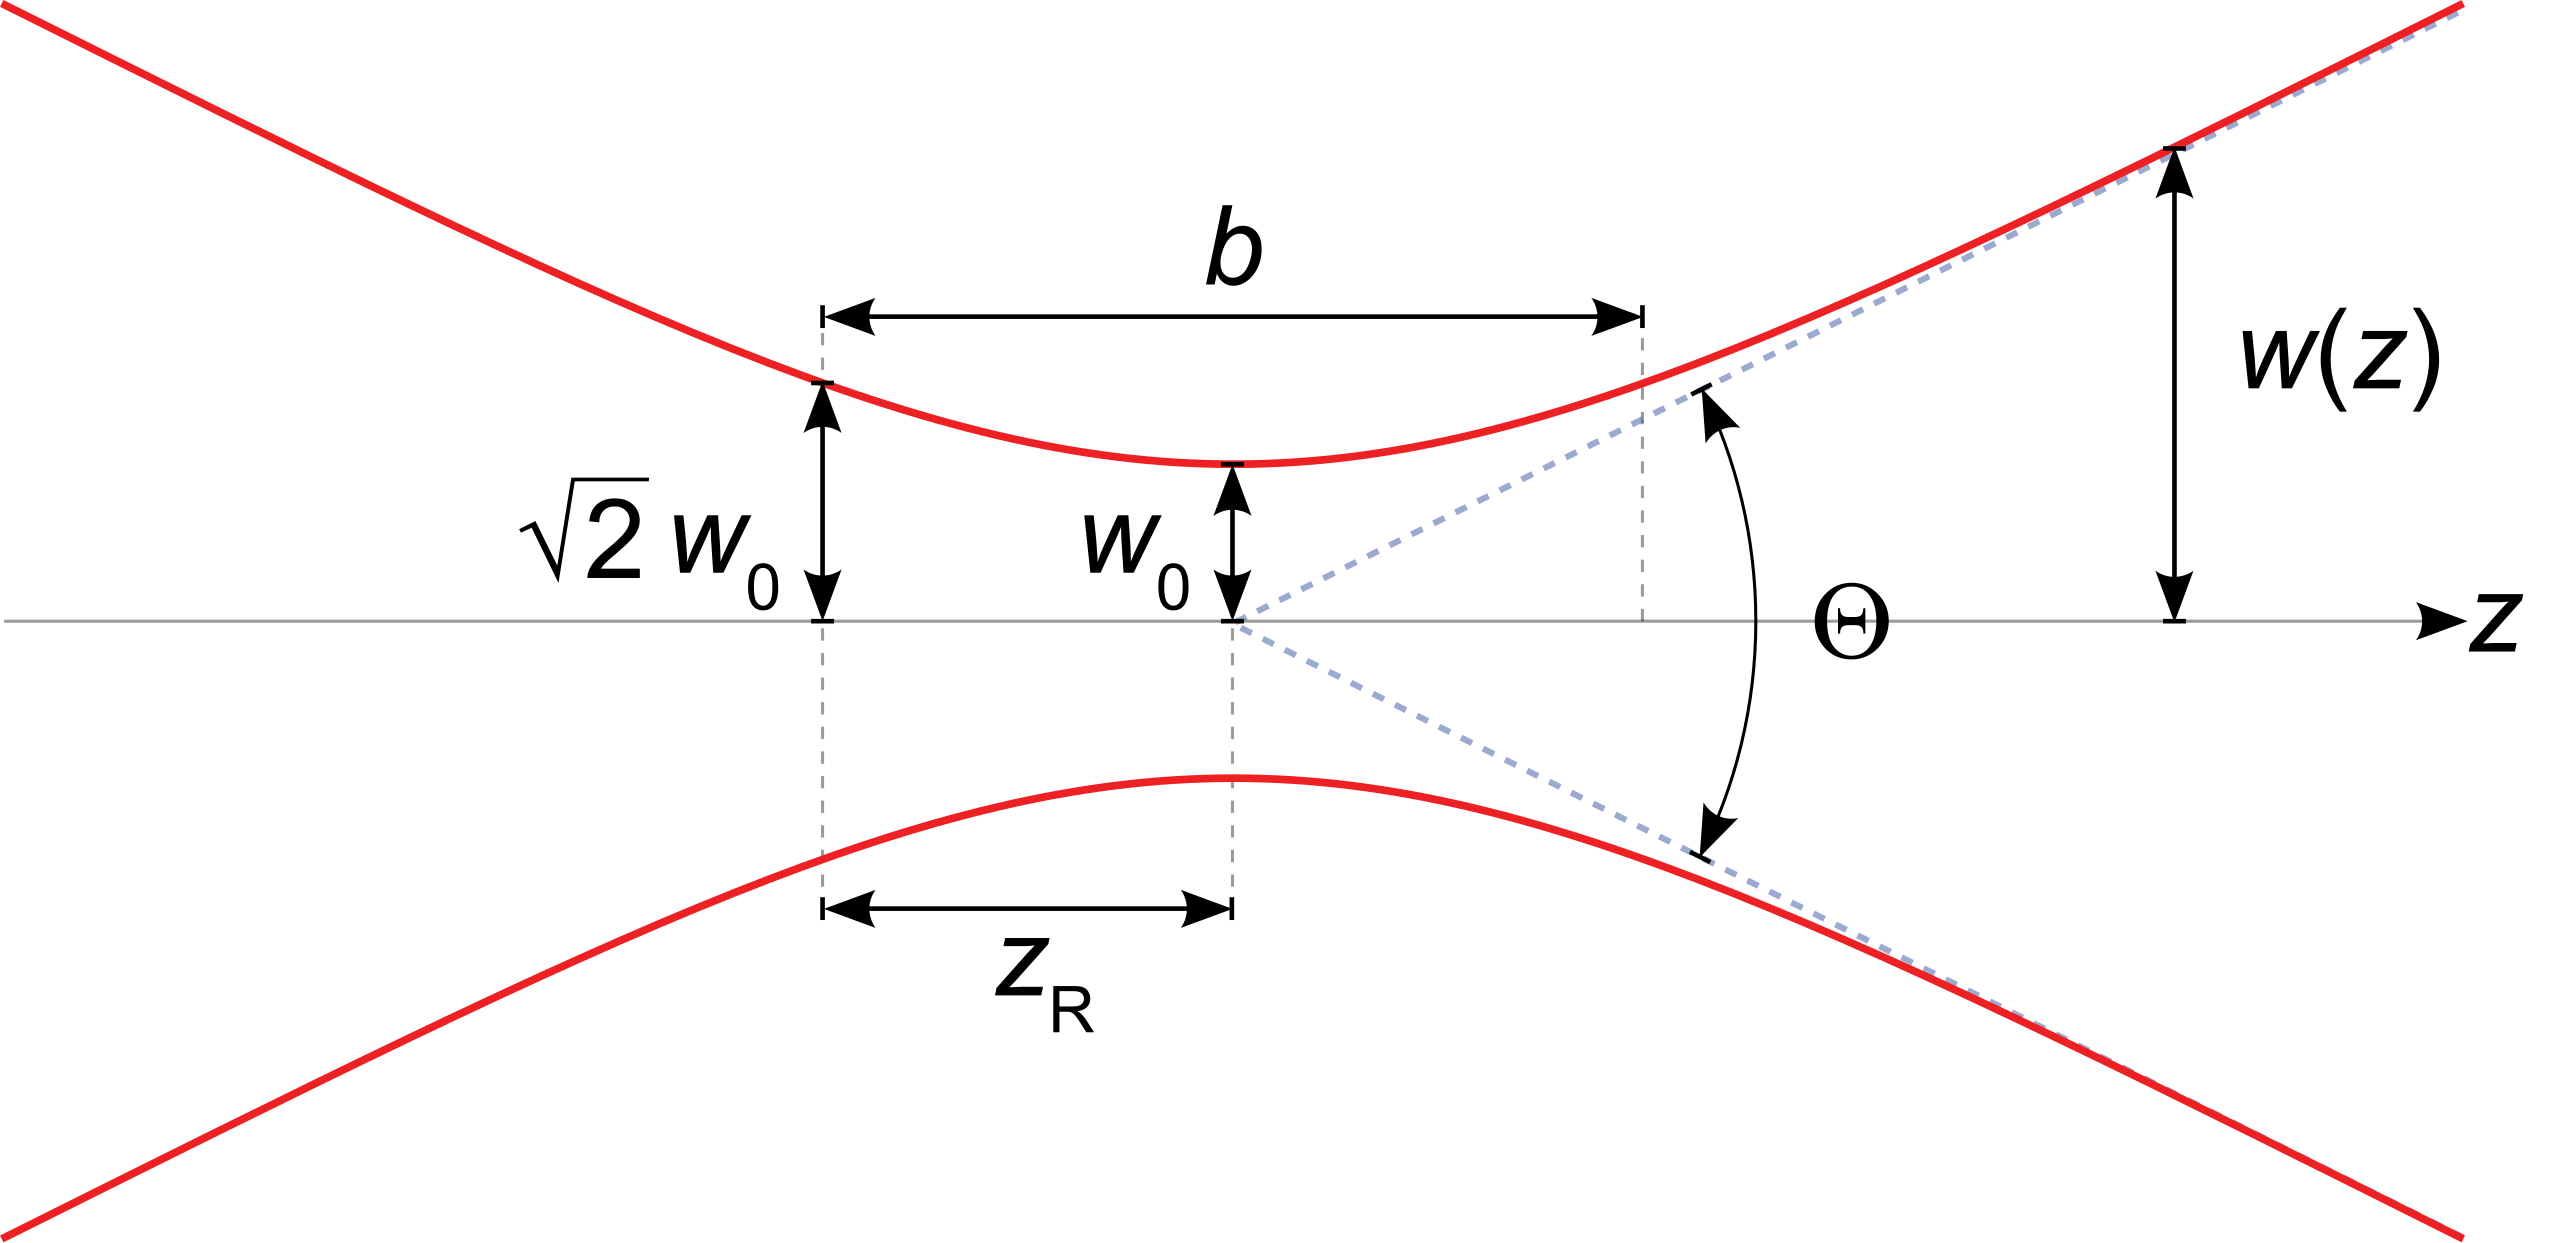
\includegraphics[scale=0.3]{gauss.png}
\end{figure}

of the form
\begin{align}
g_\Delta(x-x') = \f{1}{\sqrt{\pi \Delta^2}}e^{-(x-x')^2/\Delta^2}.
\end{align}
It is clear that the area under the curve is one (one can easily check this). Also, $\Delta \to 0$, $g_\Delta$ becomes closer and closer to $\delta(x-x')$ (the area under the curve is the same, while the width of the peak becomes smaller and smaller). 


From Gaussian model, we know that the delta function is not only real but also even:
\begin{align}
\delta(x-x') = \delta(x'-x).
\end{align}
Next, we consider the derivative of $\delta(x-x')$ with respect to $x$:
\begin{align}
\delta'(x-x') = \f{d}{dx}\delta(x-x') = -\f{d}{dx'}\delta(x-x').
\end{align}
Once again, we consider the Gaussian model. We consider $dg_\Delta(x-x')/dx = -dg_\Delta(x-x')/dx'$ as a function of $x'$:
\begin{figure}[!htb]
	\centering
	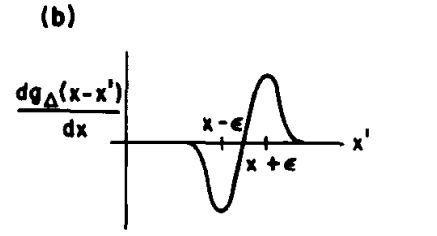
\includegraphics[scale=0.5]{dgauss.png}
\end{figure}

As $g_\Delta$ shrinks,, each bump at $\pm \epsilon$ will become, up to a scale factor, the $\delta$ function, such that
\begin{align*}
\int\delta'(x-x')f(x')\,dx' \propto   f(x+\epsilon) - f(x-\epsilon) = 2\epsilon\f{df}{dx'}\bigg\vert_{x=x'}.
\end{align*}
The constant of proportionality turns out to be $\epsilon/2$, and so
\begin{align}
\int \delta'(x-x')f(x')\,dx' = \f{df}{dx'}\bigg\vert_{x=x'} = \f{df(x)}{dx}.
\end{align}
In short, we can describe the $\delta'$ function as 
\begin{align}
\delta'(x-x') = \delta(x-x')\f{d}{dx'}.
\end{align}

In this way, we can describe higher derivatives of $\delta$:
\begin{align}
\f{d^n \delta(x-x')}{dx^n} = \delta(x-x')\f{d^n}{dx'^n}.
\end{align}



Next, we will develop an alternative representation of the delta function. Suppose we're given a function $f(x)$. The Fourier transform is given by 
\begin{align}
\F[f](k) = \f{1}{\sqrt{2\pi}}\int^\infty_{-\infty}e^{-ikx}f(x)\,dx.
\end{align}
And the inverse is given by
\begin{align}
\F^{-1}[f](x) = \f{1}{\sqrt{2\pi}}\int^\infty_{-\infty}e^{ikx'}f(k)\,dk.
\end{align}
Feeding the inverse formula into the transform formula, we get
\begin{align}
f(x') = \int^{\infty}_{-\infty} \lp \f{1}{2\pi} \int^{\infty}_{-\infty}e^{ik(x-x')\,dk} \rp f(x)\,dx.
\end{align}
Comparing this result to \eqref{delt}, we see that
\begin{align}
\boxed{\f{1}{2\pi}\int^\infty_{-\infty}e^{ik(x-x')\,dk} = \delta(x-x')}
\end{align}






\subsubsection{Operators in Infinite Dimensions}

Let us revisit the linear transformation:
\begin{align}
\Omega \ket{f} =\ket{\tilde{f}}
\end{align}
in the vector space whose basis is $\ket{x}$.

Let us assume that this action takes place in an infinite-dimensional vector space. Consider the differential operator. We can write the equation above as
\begin{align}
D_x\ket{f(x)} = \ket{df/dx}.
\end{align}

What are the matrix elements of the operator $D$ in the $\ket{x}$ basis? To find the matrix elements, we do exactly as before:
\begin{align}
\bra{x}D\ket{f} = \braket{x}{\f{df}{dx}} = \f{df(x)}{dx},
\end{align}
followed by
\begin{align}
\int \bra{x}D\ket{x'}\bra{x'}\ket{f}\,dx' = \f{df}{dx}.
\end{align}
We deduce that 
\begin{align}
\bra{x}D\ket{x'} = D_{xx'} = \delta'(x-x') = \delta(x-x')\f{d}{dx'}.
\end{align}

We notice that $D$ is not Hermitian because if
\begin{align}
D_{xx'} = D^*_{x'x}
\end{align}
then 
\begin{align}
D_{xx'} = \delta'(x-x') = D^*_{x'x} = \delta'(x'-x) = -\delta'(x-x'),
\end{align}
which is obviously not true. But we can convert $D$ to a Hermitian matrix by multiplying it with a purely imaginary number. Consider
\begin{align}
K = -iD.
\end{align}
Then
\begin{align}
K^*_{x'x} = [-i\delta'(x'-x)]^* = i\delta'(x'-x) = -i\delta'(x-x') = K_{xx'}.
\end{align}
It turns out that this is not enough to make $K$ Hermitian, as we shall show now. Suppose we have $\ket{f}$ and $\ket{g}$ in the function space whose images in the $x$ basis are $f(x)$ and $g(x)$ in the interval $a-b$. If $K$ is Hermitian, we must have that
\begin{align}
\bra{g}K\ket{f} = \bra{g}\ket{Kf} = \bra{Kf}\ket{g}^* = \bra{f}K^\dagger\ket{g}^* = \bra{f}K\ket{g}^*.
\end{align}
So, we ask
\begin{align}
\int^b_a \int^b_a \braket{g}{x}\bra{x}K\ket{x'}\braket{x'}{f}\,dx\,dx'  \stackrel{?}{=} \lp \int^b_a\int^b_a   \braket{f}{x}\bra{x}K\ket{x'}\braket{x'}{g}\,dx\,dx'  \rp^*.
\end{align}
Or, equivalently, we ask that if $K = -iD$, then
\begin{align}
 \int^b_a g^*(x)\lb -i\f{df(x)}{dx} \rb \,dx  \stackrel{?}{=}    \left\{ \int^b_a  f^*(x)\lb -i\f{dg(x)}{dx} \rb\,dx  \right\} = i\int^b_a \f{dg^*}{dx}f(x)\,dx.
\end{align}
Integrating the left hand side by parts gives
\begin{align}
-ig^*(x)f(x)\bigg\vert^b_a + i \int^b_a \f{dg^*}{dx}f(x)\,dx.
\end{align}
So for equality to hold, we require that 
\begin{align}\label{cond}
\boxed{-ig^*(x)f(x)\bigg\vert^b_a= 0}
\end{align}
Thus, in contrast to the finite-dimensional case, $K_{xx'} = K^*_{x'x}$ is not a sufficient condition for $K$ to be Hermitian. We must also look at the behavior of the functions at the end points $a$ and $b$. So what kinds of functions make this work? One set of such functions are the possible configurations $f(x)$ of the string clamped at $x=0$ and at $x=L$. These functions of course have zero boundary conditions. But this condition \eqref{cond} can also be fulfilled in another way. \\


Consider functions in 3-dimensional space, parameterized by $r,\theta,\phi$. Suppose that these functions are single-valued, say, $f(\theta) = f(\theta+2\pi)$. In the space of these functions, $K = -iD$ is Hermitian. This is very easy to verify since the condition \eqref{cond} is met:
\begin{align}
-ig^*(x)f(x)\big\vert_0^{2\pi} =-ig(2\pi)f(2\pi) + ig^*(0)f(0) = 0.
\end{align}

In quantum mechanics, we are interested in functions over the full interval $-\infty \leq x \leq \infty$. These functions into two classes: those that vanish at infinity and those that don't. Functions that don't vanish at infinity behave as $e^{-ikx}$, where $k$ is real. It is clear that if $K$ is sandwiched between two functions of the first class or two functions where one comes from each class, then $K$ is Hermitian, because the boundary terms vanish. But if $K$ is sandwiched between two functions of the second class, then whether $K$ is Hermitian depends on whether
\begin{align}
e^{ikx}e^{-ik'x}\bigg\vert_{-\infty}^\infty \stackrel{?}{=} 0.
\end{align}

If $k' = k$ then $K$ is Hermitian. If $k'\neq k$ then the answer is unclear because $e^{i(k-k')x}$ oscillates. It turns out that there exists a way of defining a limit for such functions that connect make up their minds: the limit as $\abs{x} \to \infty$. This limit is defined to be the average over a large interval. According to this prescription, we have, say as $x\to \infty$:
\begin{align}
\lim_{x\to\infty} e^{ikx}e^{-ik'x} = \lim_{L\to\infty, \Delta\to\infty}\f{1}{\Delta}\int^{L+\Delta}_L e^{i(k-k')x}\,dx = 0 \hspace{0.5cm} k\neq k'.
\end{align}
And thus $K$ is Hermitian in this space as well. \\

Next, we are interested in the eigenvalue problem of $K$. Let us start with
\begin{align}
K\ket{k} = k\ket{k}.
\end{align}
Following the standard procedure,
\begin{align}
\bra{x}K\ket{k} = k\braket{x}{k} &\implies \int \bra{x}K\ket{x'}\bra{x'}\ket{k}\,dx' = k\psi_k(x)\\ &\implies -i\f{d}{dx}\psi_k(x) = k\psi_k(x)
\end{align}
where $\psi_k(x) = \braket{x}{k}$. This is a very simple differential equation whose solution is
\begin{align}
\psi_k(x) = Ae^{ikx}.
\end{align}
Let us chose $A$ to be such that the function is normalized. In this case $A = 1/\sqrt{2\pi}$. And so,
\begin{align}
\ket{k} \sim \f{1}{\sqrt{2\pi}} e^{ikx},
\end{align}
and
\begin{align}
\braket{k}{k'} = \int^\infty_{-\infty} \braket{k}{x}\braket{x}{k'}\,dx = \f{1}{2\pi}\int^\infty_{-\infty}e^{-i(k-k')x}\,dx = \delta(x-x').
\end{align}


Now, because $K$ is Hermitian, functions that are expanded in the $x$ basis with components $f(x) = \braket{x}{f}$ must also have an expansion in the $K$ basis. What are the components in this expansion? We first look at the components in the $K$ basis, starting with $\ket{k}$:
\begin{align}
f(k) = \braket{k}{f} = \int^\infty_{-\infty} \braket{k}{x}\braket{x}{f}\,dx = \f{1}{\sqrt{2\pi}}\int^\infty_{-\infty} e^{-ikx}f(x)\,dx. 
\end{align}
To get back to the $x$ basis, we simply apply the inverse transform:
\begin{align}
f(x) = \braket{x}{f} = \int^\infty_{-\infty}   \braket{x}{k}\braket{k}{f}\,dk = \f{1}{\sqrt{2\pi}}\int^\infty_{-\infty} e^{ikx}f(k)\,dk.
\end{align}
Thus the familiar Fourier transform gives us the passage from one complete basis to another. What about the matrix elements of $K$ in the $k$ basis? It turns out that these elements are trivial:  
\begin{align}
\bra{k}K\ket{k'} = k'\braket{k}{k'} = k'\delta(k-k').
\end{align}
So, the $k$ basis is generated by the Hermitian operator $K$. So what generates the $x$ basis? Let us call this operator $X$, and that 
\begin{align}
X\ket{x} = x\ket{x}. 
\end{align}
Its matrix elements in the $x$ basis are
\begin{align}
\bra{x'}X\ket{x} = x\delta(x'-x).
\end{align}
To find its actions on functions, let us define
\begin{align}
X\ket{f} = \ket{\tilde{f}}.
\end{align}
And so
\begin{align}
\bra{x}X\ket{f} = \int  \bra{x}X\ket{x'}\bra{x'}\ket{f}\,dx' = xf(x) = \braket{x}{\tilde{f}} = \tilde(f)(x).
\end{align}
Therefore,
\begin{align}
\tilde{f}(x) = xf(x).
\end{align}
So, $X$ has the effect of multiplying a function $f$ by $x$:
\begin{align}
X\ket{f(x)} = \ket{xf(x)}.
\end{align}
We notice that there is a nice reciprocity between $X$ and $K$. Let us compute the matrix elements of $X$ in the $k$ basis:
\begin{align}
\bra{k}X\ket{k'} &= \f{1}{2\pi}\int^\infty_{-\infty} e^{-ikx} x e^{ik'x} \,dx \\
&= i\f{d}{dk} \lp \f{1}{2\pi}\int^\infty_{-\infty} e^{i(k'-k)x}\,dx \rp = i\delta'(k-k').
\end{align}
So, if $\ket{g(k)}$ is a ket whose image in the $k$ basis is $g(k)$ then
\begin{align}
X\ket{g(k)} = \ket{\f{idg(k)}{dk}}.
\end{align}

Thus we have the following. In the $x$ basis, $X$ acts as $x$. In the $k$ basis, $X$ acts as $-id/dx$. On the other hand, in the $k$ basis, $K$ acts as $k$, and in the $x$ basis as $-id/dk$. Operators with such an interrelationship are said to be \textbf{conjugate} of each other. Now, the conjugate operators $K$ and $X$ don't commute. Let us calculate their commutator. Suppose we have some ket $\ket{f}$. Then,
\begin{align}
&X\ket{f} \to xf(x)\\
&K\ket{f} \to -i\f{df(x)}{dx}.
\end{align} 
This is just the definition of these operators. Next,
\begin{align}
&XK\ket{f} \to -i x \f{df(x)}{dx}\\
&KX\ket{f} \to -i\f{d}{dx}xf(x).
\end{align}
Thus, 
\begin{align}
[X,K]\ket{f} \to -i x \f{df(x)}{dx} + i x \f{df(x)}{dx} + if \to i\Id\ket{f}.
\end{align}
So, we have for $X$ and $K$ conjugate of each other,
\begin{align}
[X,K] = i\Id.
\end{align}
























































\newpage


\section{Review of Classical Mechanics}


\subsection{Principle of Least Action \& Lagrangian Mechanics}

Suppose we have a particle in a potential $V(x)$. Newton tells us that
\begin{align}
m\f{d^2 x}{dt^2} = -\f{dV}{dx}.
\end{align}
In general coordinates,
\begin{align}
m_j \f{d^2x_j}{dt^2} = -\f{\p V}{\p x_j}.
\end{align}
In Lagrangian mechanics, we first define the \textit{Lagrangian}: $\lag = T - V$, where $T$ is the kinetic energy and $V$ is the potential energy. This makes $\lag = \lag(x,\dot{x},t)$. For each path connecting $(x_i,t_i)$ to $(x_f,t_f)$, the \textit{action} is given by
\begin{align}
S[x(t)] = \int^{t_f}_{t_i} \lag(x,\dot{x})\,dt.
\end{align}
The classical path which the particle follows is one which minimizes $S[x(t)]$. Variational methods (requiring $\delta S = 0$ and boundary terms to vanish) give us the \textbf{Euler-Lagrange equation(s)}:
\begin{align}
\boxed{\f{\p \lag}{\p x(t)} = \f{d}{dt}\f{\p \lag}{\p \dot{x}(t)}}
\end{align}
Details of this derivation can be found in many differential equation textbooks. We can easily show how Newton's Second law emerges from the Euler-Lagrange equation by setting $T = mv^2/2$. In which case, we get
\begin{align}
\f{d}{dt}(m\dot{x}) = m\ddot{x}= -\f{dV}{dx}.
\end{align}  
In general coordinates, we get the same thing:
\begin{align}
m\ddot{x}_{i} = -\f{\p V}{\p x_i}.
\end{align}
Now, we notice that we have assumed the potential $V$ to be velocity-independent. The force of a magnetic field $\mathbf{B}$ on a moving charge is excluded by this restriction ($\mathbf{F} = q\mathbf{v}\times \mathbf{B}$). We will show shortly how to accommodate this force in the Lagrangian formalism. However, this treatment will leave $\lag$ no longer in the form $T - V$. So, we will be free from the notion that $\lag$ has the form $T-V$, by only requiring that $\lag$ gives the correct equations of motion.

Suppose in some generalized coordinates, we have
\begin{align}
\f{d}{dt}\lp \f{\p \lag}{\p \dot{q}_i} \rp = \f{\p \lag}{\p q_i}.
\end{align}
It turns out that the \textit{form} of the Euler-Lagrange equation is invariant under change of coordinates. The Euler-Lagrange equation above can be made to resemble Newton's Second law if one defines a quantity:
\begin{align}
p_i = \f{\p \lag}{\p \dot{q}_i}
\end{align}
as the \textbf{canonical momentum conjugate to $q_i$} and the quantity
\begin{align}
F_i = \f{\p \lag}{\p q_i}
\end{align}
as the \textit{generalized force conjugate to $q_i$}. Note that these quantities are not always linear momentum and force. They can be angular momentum and torque, for instance. In many cases, we can find conservation laws from the Lagrangian, but we won't go into the details for now.









\subsection{The Electromagnetic Lagrangian}
As promised, in this subsection we will incorporate electromagnetism into the Lagrangian formalism. Recall that the force on a charge $q$ due to an electric field $\mathbf{E}$ and a magnetic field $\mathbf{B}$ is given by
\begin{align}
\boxed{\mathbf{F} = q\lp \mathbf{E} + \f{\mathbf{v}}{c}\times \mathbf{B} \rp}
\end{align}
where $\mathbf{v} = \dot{\mathbf{r}}$ is the velocity of the charged particle, and $c$ is the speed of light. It turns out that if we use 
\begin{align}
\boxed{\lag_{EM} = \f{1}{2}m\mathbf{v}\cdot\mathbf{v} - q\phi + \f{q}{c}\mathbf{v}\cdot\mathbf{A}}
\end{align}
we get the correct electromagnetic force laws. We note that $\phi$ and $\mathbf{A}$ are the scalar and the vector potentials related to $\mathbf{E}$ and $\mathbf{B}$ via:
\begin{align}
\mathbf{E} = -\grad{\phi} - \f{1}{c}\f{\p \mathbf{A}}{\p t}
\end{align}
and 
\begin{align}
\mathbf{B} = \curl{\mathbf{A}}.
\end{align}
With respect to this Lagrangian, the Euler-Lagrange equation is
\begin{align}
\f{d}{dt}\lp mx_i + \f{q}{c}\mathbf{A}_i \rp = -q\f{\p\phi}{\p x_i} + \f{q}{c}\f{\p \mathbf{v}\cdot\mathbf{A}}{\p x_i}.
\end{align}
We can combine the $i=1,2,3$ equations into one vector equation:
\begin{align}
\f{d}{dt}\lp m\mathbf{v} + \f{q\mathbf{A}}{c} \rp = -q\grad{\phi} + \f{q}{c}\grad{(\mathbf{v}\cdot\mathbf{A})}.
\end{align}
Rewriting this gives
\begin{align}
\f{d}{dt}m\mathbf{v} = -q\grad{\phi} + \f{q}{c}\lb -\f{d\mathbf{A}}{dt} + \grad{(\mathbf{v}\cdot\mathbf{A})} \rb
\end{align}


The canonical momentum is then
\begin{align}
\mathbf{p} = \f{\p \lag}{\p \dot{\mathbf{x}}} = m\mathbf{v} + \f{q\mathbf{A}}{c}. 
\end{align}
Now, the total derivative $d\mathbf{A}/dt$ has two parts:
\begin{align}
\f{d\mathbf{A}}{dt} = \f{\p \mathbf{A}}{\p t} + (\mathbf{v}\cdot \grad)\mathbf{A} 
\end{align}
where
\begin{align}
\lp\mathbf{v}\cdot\grad\rp_i = \f{dx_i}{dt}\f{\p}{\p x_i}.
\end{align}
Thus we have
\begin{align}
\f{d}{dt}m\mathbf{v} = -q\grad{\phi} - \f{q}{c}\f{\p \mathbf{A}}{\p t} + \f{q}{c}\lb \grad{(\mathbf{v}\cdot \mathbf{A})} - (\mathbf{v}\cdot \grad)\mathbf{A} \rb.
\end{align}
Now, we use the identity
\begin{align}
\mathbf{v}\times (\curl{A}) = \grad{(\mathbf{v}\cdot \mathbf{A})} - (\mathbf{v}\cdot \grad)\mathbf{A}
\end{align}
to get
\begin{align}
\f{d}{dt}m\mathbf{v} = -q\grad{\phi} - \f{q}{c}\f{\p \mathbf{A}}{\p t} + \f{q}{c}\mathbf{v}\times (\curl{A}).
\end{align}
Using the definition of $\mathbf{E}$ and $\mathbf{B}$ in relation to $\phi$ and $\mathbf{A}$ we indeed get the correct force law:
\begin{align}
\f{d}{dt}m\mathbf{v} = \mathbf{F} = q\lp \mathbf{E} + \f{\mathbf{v}}{c}\times\mathbf{B} \rp
\end{align}





\subsection{The two-body problem}
The two-body problem can be solved more elegantly in the \textit{center-of-mass coordinate system} where
\begin{align}
\mathbf{r} = \mathbf{r}_1 - \mathbf{r}_2
\end{align}
and 
\begin{align}
\mathbf{r}_{CM} = \f{m_1\mathbf{r}_1 + m_2\mathbf{r_2}}{m_1 + m_2}.
\end{align}
The inverse formulas are as follow:
\begin{align}
&\mathbf{r}_1 = \mathbf{r}_{CM} + \f{m_2\mathbf{r}}{m_1 + m_2}\\
&\mathbf{r}_2 = \mathbf{r}_{CM} - \f{m_1\mathbf{r}}{m_1 + m_2}
\end{align}
The original Lagrangian is
\begin{align}
\lag = \f{1}{2}m_1\abs{\dot{\mathbf{r}}_1}^2 + \f{1}{2}m_2\abs{\dot{\mathbf{r}}_2}^2 - V(\mathbf{r}_1 - \mathbf{r}_2). 
\end{align}
In CM coordinate system, the Lagrangian becomes:
\begin{align}
\lag =\f{1}{2}(m_1 + m_2)\abs{\dot{\mathbf{r}}_{CM}}^2 + \f{1}{2}\f{m_1m_2}{m_1+m_2}\abs{\mathbf{r}}^2 - V(\mathbf{r}).
\end{align}
By doing this, we have in a sense ``decoupled'' the problem:
\begin{align}
\lag(\mathbf{r},\dot{\mathbf{r}}, \mathbf{r}_{CM}, \dot{\mathbf{r}}_{CM},t) = \lag(\mathbf{r},\dot{\mathbf{r}},t) + \lag(\mathbf{r}_{CM}, \dot{\mathbf{r}}_{CM},t).
\end{align}
The first fictitious particle is the center of mass of the system. The motion of the center of mass is often uninteresting, so we can always go to the center of mass frame, so that the term $\lag(\mathbf{r}_{CM}, \dot{\mathbf{r}}_{CM},t)$ vanishes completely from the total Lagrangian. The second fictitious particle has \textit{reduced mass}:
\begin{align}
\mu = \f{m_1m_2}{m_1+m_2}
\end{align}
moves under the potential $V(\mathbf{r})$. Now, we only need to solve this one-body problem. 


\subsection{The Hamiltonian Formalism}
Recall the canonical momentum in Lagrangian mechanics:
\begin{align}
p_i = \f{\p \lag}{\p \dot{q}_i}.
\end{align}

In the Hamiltonian formalism one exchanges the roles of $\dot{q}$ and $p$: one replaces the Lagrangian $\lag(q,\dot{q})$ by a Hamiltonian $\ham(q,p)$ which generates the equations of motion, and $\dot{q}$ becomes a derived quantity:
\begin{align}
\dot{q}_i = \f{\p \ham}{\p p_i}.
\end{align}
But of course the question is, how can we make such a change? It turns out that there exists procedure for effecting such a change, called a \textit{Legendre transformation}. Suppose we have a function $f(x)$ with
\begin{align}
u(x) = \f{df(x)}{dx}.
\end{align}
How do we invert $u(x)$ to get $x(u)$? If we define a function (called the \textbf{Legendre transformation})
\begin{align}
\boxed{g(u) = x(u)u - f(x(u))}
\end{align}
then
\begin{align}
\f{dg}{du} = \f{dx}{du}u + x(u) - \f{df}{dx}\f{dx}{du} = x(u).
\end{align}
In going from $f$ to $g$, we simply exchange the roles of $x$ and $u$. $f$ and $g$ are called the Legendre transforms of each other. More generally, if $f = f(x_1,\dots,x_n)$, one can eliminate a subset $\{x_i\}$ in favor of the partial derivatives $u_i = \p f/\p x_i$ by the transformation
\begin{align}
g(u_1,\dots,u_j,x_{j+1},\dots,x_{n}) = \sum^j_{i=1}u_ix_i - f(x_1,\dots,x_n).
\end{align}
We can easily check that 
\begin{align}
\f{\p g}{\p u_i} = x_i.
\end{align}
So, we define the Hamiltonian as
\begin{align}
\boxed{\ham(q,p) = \sum^n_{i=1}p_i \dot{q}_i - \lag(q,\dot{q})}
\end{align}
where the $\dot{q}$'s are functions of $p$'s and $q$'s. Now, we observe that
\begin{align}
\f{\p \ham}{\p p_i} &= \f{\p }{\p p_i}\lp \sum^n_{j=1}p_j \dot{q}_j - \lag(q,\dot{q})  \rp\\
&= \dot{q}_i + \sum_{j=1}^n p_j \f{\p \dot{q}_j}{\p p_i} - \sum_{j=1}^n \underbrace{\f{\p \lag}{\p \dot{q}_j}}_{p_j}\f{\p \dot{q}_j}{\p p_i}\\
&= \dot{q}_i.
\end{align}
Similarly, we have that
\begin{align}
\f{\p \ham}{\p q_i} &= \f{\p }{\p q_i}\lp \sum^n_{j=1}p_j \dot{q}_j - \lag(q,\dot{q})  \rp\\
&= \sum_j p_j\f{\p \dot{q}_j}{\p q_i} - \f{\p \lag}{\p q_i} 
- \sum_j \underbrace{\f{\p \lag}{\p \dot{q}_j}}_{p_j}\f{\p \dot{q}_j}{\p p_i}
\\
&=-\f{\p \lag}{\p q_i}.
\end{align}
We obtain the \textit{Hamilton's canonical equations} by replacing $\p \lag / \p q_i$ by $\dot{p}_i$:
\begin{align}
\boxed{\f{\p \ham}{\p p_i} = \dot{q}_i, \hspace{0.5cm} -\f{\p \ham}{\p q_i} = \dot{p}_i}
\end{align}
We have altogether $2n$ first-order equations in time for a system with $n$ degrees of freedom. Given $(q_i(0), p_i(0))$ it is possible to integrate to find $(q_i(t), p_i(t))$.\\

Let us take a moment now to compare Lagrangian and Hamiltonian mechanics.\\

\noindent 
\begin{tabular}{|p{5.5cm}|p{5.5cm}|}
	\hline
	\textbf{Lagrangian formalism} & \textbf{Hamiltonian formalism}\\
	\hline
	The state of a system with $n$ df's is described by $n$ coordinates $(q_1,\dots,q_n)$ and $n$ velocities $(\dot{q}_1,\dots,\dot{q}_n)$, or in a more compact notation by $(q_i, \dot{q}_i)$. & The state of a system with $n$ df's is described by $n$ coordinates and $n$ momenta $(q_1,\dots,q_n; p_1, \dots, p_n)$ or, more succinctly, $(q,p)$.\\
	\hline
	The state of the system may be represented b a point moving with a definite velocity in an $n$-dimensional configuration space. & The state of the system nay be represented by a point in $2n$-dimensional phase space with coordinates $(q_1,\dots,q_n; p_1, \dots, p_n)$.\\
	\hline
	The $n$ coordinates evolve according to $n$ second-order equations.&The $2n$ coordinates and momenta obey $2n$ first-order equations.\\
	\hline
	For a given $\lag$, several trajectories may pass through a given point in configuration space depending on $\dot{q}$. & For a given $\ham$ only one trajectory passes through a given point in phase space.\\
	\hline
\end{tabular}\\



So what is $\ham$, physically? We know that $\lag$ can be interpreted as $T - V$ if the force is conservative. Let us looks at $\ham$ for this case. Suppose
\begin{align}
T &= \sum_{i=1}^n \f{1}{2}m_i \dot{x}_i^2 \\ p_i &= \f{\p \lag}{\p \dot{x}_i} = \f{\p T}{\p \dot{x}_i} = m_i \dot{x}_i,
\end{align}
where the coordinates are Cartesian $q_i = x_i$. This gives
\begin{align}
\ham 
&= \sum^n_{i=1}p_i \dot{x}_i - \lag(q,\dot{x})\\
&= \sum^n_{i=1}m_i \dot{x}_i^2 - \lag(q,\dot{x})\\
&= 2T - \lag\\
&= T + V.
\end{align}
So, we can interpret $\ham$ as the total energy (assuming that the force is conservative). Of course, we also assumed that the potential is not velocity-dependent, which does not apply to electromagnetism. In the next section, we will look into electromagnetism in the Hamiltonian scheme.
















\subsection{The Electromagnetic Force in the Hamiltonian Scheme}
Recall the Lagrangian for electromagnetism:
\begin{align}
\lag_{EM} = \f{1}{2}m\mathbf{v}\cdot\mathbf{v} -q\phi + \f{q}{c}\mathbf{v}\cdot\mathbf{A}
\end{align}
where 
\begin{align}
\mathbf{p} = m\mathbf{v} + \f{q\mathbf{A}}{c}.
\end{align}
In the Hamiltonian scheme, we write
\begin{align}
\ham_{EM} 
&= \mathbf{p}\cdot \mathbf{v} - \lag_{EM} \\
&= \lp m\mathbf{v} + \f{q\mathbf{A}}{c} \rp \cdot \mathbf{v} - \lp \f{1}{2}m\mathbf{v}\cdot\mathbf{v} -q\phi + \f{q}{c}\mathbf{v}\cdot\mathbf{A} \rp\\
&= \f{1}{2}m\mathbf{v}\cdot\mathbf{v} + q\phi\\
&= T + q\phi.
\end{align}
Wait a minute. What's happened to the vector potential $\mathbf{A}$? How can $\ham_{EM}$ generate the correct dynamics without knowing $\mathbf{A}$? It turns out that $T$ is dependent on $\mathbf{p}$ and $\mathbf{A}$. Recall that
\begin{align}
\f{1}{2}m\mathbf{v}\cdot\mathbf{v} = T = \f{\abs{\mathbf{p} - q\mathbf{A}/c}^2}{2m}.
\end{align}
Thus we have
\begin{align}
\boxed{\ham_{EM} = \f{\abs{\mathbf{p} - q\mathbf{A}/c}^2}{2m} + q\phi}
\end{align}





\subsection{Cyclic Coordinates, Poisson Brackets, and Canonical Transformations}
Let a Hamiltonian $\ham(q,p)$ be given. Suppose that the coordinate $q_i$ is missing in $\ham$, then 
\begin{align}
\dot{p}_i = -\f{\p \ham}{\p q_i} = 0,
\end{align}
which means the canonical momentum $p_i$ is conserved. Now, in many cases there are other quantities that are conserved, such as energy. How do we characterize these in the Hamiltonian formalism? It turns out there is a way to do this. \\

Suppose $\omega(q,p)$ is some state variable that doesn't depend explicitly on time $t$. Then we have by the chain rule
\begin{align}
\f{d\omega}{dt} 
&= \sum_i \lp \f{\p \omega}{\p q_i}\dot{q}_i + \f{\p \omega}{\p p_i}\dot{p}_i \rp\\
&= \sum_i \lp \f{\p \omega}{\p q_i}\f{\p \ham}{\p p_i} - \f{\p \omega}{\p p_i}\f{\p \ham}{\p q_i} \rp\\
&\equiv \{ \omega, \ham \}.
\end{align}
So, we define the Poisson bracket between two variables $\omega(q,p)$ and $\lambda(q,p)$ to be
\begin{align}
\boxed{\{\omega,\lambda\} = \sum_i \lp \f{\p \omega}{\p q_i}\f{\p \lambda}{\p p_i} - \f{\p \omega}{\p p_i}\f{\p \lambda}{\p q_i} \rp}
\end{align}

Let us look at this equation again
\begin{align}
\f{d\omega}{dt} = \sum_i \lp \f{\p \omega}{\p q_i}\f{\p \ham}{\p p_i} - \f{\p \omega}{\p p_i}\f{\p \ham}{\p q_i} \rp = \{ \omega, \ham \}
\end{align}
This says that any state variable whose Poisson bracket with $\ham$ vanishes is constant in time (i.e., is a conserved quantity). \\

Poisson brackets have a few important properties and similarities with commutators:
\begin{enumerate}
	\item $\{\omega, \lambda\} = -\{ \lambda,\omega    \}$
	\item $\{\omega, \lambda + \sigma \} = 
	\{\omega, \lambda  \}
	+
	\{\omega,  \sigma \}$
	\item $\{\omega, \lambda \sigma \} = 
	\{\omega, \lambda  \}\sigma
	+
	\lambda\{\omega,  \sigma \}$
	\item $\{ q_i,q_j \} = \{ p_i , p_j \} = 0$
	\item $\{ q_i, p_j  \} = \delta_{ij}$
	\item $\dot{q}_i = \{ q_i,\ham   \}$
	\item $\dot{p}_i = \{ p_i,\ham   \}$
\end{enumerate}

Please refer to Shankar's book for the sections on \textit{Canonical Transformations, Active Transformations, and Symmetries and Their Consequences}.

%\subsubsection{Canonical Transformations}
%\subsubsection{Active Transformations}
%\subsection{Symmetries and Their Consequences}
%\subsubsection{A Useful Relation between $\mathbf{S}$ and $\mathbf{E}$}




\newpage




%\section{All is Not Well with Classical Mechanics}
%\subsection{Particles and Waves in Classical Physics}
%\subsection{An Experiment with Waves and Particles (classical)}
%\subsection{The Double-Slit Experiment with Light}
%\subsection{Matter Waves (de Broglie Waves)}
%
%
%\newpage



\section{The Postulates \textendash a General Discussion}

\subsection{The Postulates}

Here we introduce the postulates of nonrelativistic quantum mechanics. We consider a system with one df (a particle in one dimension). The straightforward generalization to more particles in higher dimension will be introduced later. \\

\noindent
\begin{tabular}{|p{4cm}|p{7.2cm}|}
	\hline
	\textbf{Classical Mechanics} & \textbf{Quantum Mechanics}\\ \hline
	The state of a particle at any given time is specified by the two variables $x(t)$ and $p(t)$, i.e., as a point in a two-dimensional phase space. & The state of the particle is represented by a vector $\ket{\phi(t)}$ in a Hilbert space.\\ \hline
	Every dynamical variable $\omega$ is a function of $x$ and $p$: $\omega = \omega(x,p)$. & The independent variables $x$ and $p$ of classical mechanics are represented by Hermitian operators $X$ and $P$ with the following matrix elements in the eigenbasis of $X$: \begin{equation}
	\bra{x}X\ket{x'} = x\delta(x-x')
	\end{equation}
	\begin{equation}
	\bra{x}P\ket{x'}= -i\hbar\delta'(x-x').
	\end{equation}
	The operators corresponding to dependent variables $\omega(x,p)$ are given Hermitian operators
	\begin{equation} 
	\Omega(X,P) = \omega(x\to X, p \to P).
	\end{equation}\\ \hline
	If the particle is in a state given by $x$ and $p$, the measurement of the variable $\omega$ will yield a value $\omega(x,p)$. The state will remain unaffected. & If the particle is in a state $\ket{\psi}$, measurement of the variable corresponding to $\Omega$ will yield one of the eigenvalues $\omega$ with probability $P(\omega)\propto \abs{\braket{\omega}{\psi}}^2$. The state of the system will change from $\ket{\psi}$ to $\ket{\omega}$ as a result of the measurement.\\ \hline
	The state variables change with time according to Hamilton's equations: 
	\begin{equation}
	\dot{x} = \f{\p \ham}{\p \dot{p}}
	\end{equation}
	\begin{equation}
	\dot{p} = -\f{\p \ham}{\p x}
	\end{equation}
	&
	The state vector $\ket{\psi(t)}$ obeys the Schr\"{o}dinger equation 
	\begin{equation}
	i\hbar\f{d}{dt}\ket{\psi(t)} = H\ket{\psi(t)}
	\end{equation}
	where $H(X,P)=\ham(x\to X, p\to P)$ is the quantum Hamiltonian operator and $\ham$ is the Hamiltonian for the corresponding classical problem.\\\hline
\end{tabular}


\subsubsection{Collapse of the State Vector}
Suppose we have a state vector written in a general form

\begin{align}
\ket{\psi} = \sum_\omega \ket{\omega}\bra{\omega}\ket{\psi}
\end{align}
where $\ket{\omega}$ are of course the eigenstates. We recall that this expression is equivalent to writing $\ket{\psi}$ as a linear combination of the eigenstates $\ket{\omega}$ (where the corresponding eigenvalues are $\epsilon$), with coefficients being the inner product of $\ket{\psi}$ and $\ket{\omega}$, which we can think of as ``how much of $\ket{\psi}$ is in a certain $\ket{\omega}$'' direction. \\

Now, postulate III says that the measurement of the variable $\Omega$ changes the state vector. This phenomenon is called the \textit{collapse/reduction of the state vector}. There are two types of measurements in quantum mechanics. Loosely speaking, an \textit{ideal measurement} of $\Omega$ leaves only the eigenstates of $\Omega$ invariant. For example, \textit{ideal measurement} of the momentum of a particle in a momentum eigenstate leaves the state vector of the particle unchanged. Physically, this is due to the fact that the photons required for this measurement can be infinitesimally low in energy. On the contrary, suppose we want to \textit{ideally} measure the position of some particle in a momentum eigenstate $\ket{p}$, which we can write in terms of the position eigenstates as
\begin{align}
\ket{p} =\int \ket{x} {p}\,dx.
\end{align}
We see that the measurement forces the particle into some eigenstate $\ket{x}$, thus changing the state vector. 



\subsubsection{Expectation Value}

Suppose we want to measure a variable $\Omega$, given a large ensemble of $N$ particles in a state $\ket{\psi}$. Quantum theory allows us to predict how much of the population will yield some eigenvalue $\omega$. However, often we are interested in the \textit{expectation value} of these measurements, which is defined in statistics as
\begin{align}
\langle \Omega \rangle = \sum_i  \omega_i P(\omega_i).
\end{align}
But of course each probability is the modulus square of inner product of $\ket{\psi}$ and $\ket{\omega}$. So we can write the expectation value as
\begin{align}
\langle \Omega \rangle = \sum_i \omega_i \abs{\bra{\omega_i}\ket{\psi}}^2 = \sum_i \omega_i \braket{\psi}{\omega_i}\braket{\omega_i}{\psi}.
\end{align}
Now, because each $\omega_i$ is an eigenvalue corresponding to an eigenfunction $\ket{\omega_i}$ in the eigenvalue equation $\Omega\ket{\omega_i} = \omega_i\ket{\omega_i}$, we can rewrite the equation above as
\begin{align}
\sum_i  \bra{\psi}\Omega\ket{\omega_i} \braket{\omega_i}{\psi} = \bra{\psi} \Omega \lp\sum_i \ket{\omega_i}\bra{\omega_i}\rp \ket{\psi} = \bra{\psi}\Omega\ket{\psi},
\end{align}
by completeness. Thus, 
\begin{align}
\boxed{\langle \Omega \rangle = \bra{\psi}\Omega\ket{\psi}}
\end{align}
So, we notice a few things:
\begin{enumerate}
	\item To calculate $\langle \Omega \rangle$, we only need the operator $\Omega$. We do not need to know the eigenstates nor the eigenvalues of $\Omega$. 
	\item If the particles is in some eigenstate $\ket{\omega_i}$ of $\Omega$, then $\langle \Omega \rangle = \omega_i$, the corresponding eigenvalue. 
	\item $\langle \Omega \rangle$ is not necessarily one of the eigenvalues $\omega_i$. 
\end{enumerate}





\subsubsection{The Uncertainty}

Beside the mean (or the expectation value), another useful quantity to specify is the \textit{standard deviation}, or the \textit{uncertainty}. Statistically, it is defined as
\begin{align}
\Delta \Omega = \sqrt{\langle \Omega^2 \rangle - \langle \Omega \rangle^2}.
\end{align}
In quantum mechanics, if $\Omega$ has a discrete spectrum, then the uncertainty in $\Omega$ is given by
\begin{align}
\boxed{\Delta \Omega= \sqrt{ \sum_i P(\omega_i) (\omega_i - \langle \Omega \rangle)^2  }}
\end{align}
Else if it has a continuous spectrum, then
\begin{align}
\boxed{\Delta \Omega  = \sqrt{\int P(\omega)(\omega - \langle \Omega\rangle)^2\,d\omega}}
\end{align}
Or equivalently, we can write the uncertainty in $\Omega$ as a square root of an expectation value (this is all statistical definitions, by the way):
\begin{align}
\boxed{\langle \Omega\rangle = \sqrt{ \bra{\psi}  (\Omega - \langle \Omega \rangle)^2  \ket{\psi}}}
\end{align}










\subsubsection{Compatible and Incompatible Variables}


Suppose we want to measure some quantity $\Omega$ from the state $\ket{\psi}$. Such a measurement can yield an eigenvalue, say $\omega$, with probability $P(\omega)= \abs{\braket{\omega}{\psi}}^2$ where $\ket{\omega}$ is the eigenfunction corresponding to the eigenvalue $\omega$. Now, what if we want to measure a different variable, say $\Lambda$, on the already measured state $\ket{\psi}$? We see that this is sort of like a filtering process where we start with $\ket{\psi}$ and want to produce a state with $\omega$ and $\lambda$. But notice that once we measure $\ket{\psi}$, we have made the transformation $\ket{\psi} \to \ket{\omega}$. Can measuring $\ket{\omega}$ give $\ket{\lambda}$? The answer is no, not generally, since $\ket{\omega}$ must has a component that is the eigenfunction corresponding to the eigenvalue $\ket{\lambda}$. \\

An exception occurs when the state produced after the first measurement is unaffected by the second measurement, i.e., $\ket{\omega}$ is also an eigenstate of $\Lambda$. So, a natural question is when do two operators $\Omega$ and $\Lambda$ have \textit{exactly} the same eigenkets? Mathematically, we want to know when the following equation 
\begin{align}
[\Omega, \Lambda] = 0 \forall \text{ eigenket}
\end{align}
holds. Well, given any two operators $\Omega$ and $\Lambda$, we call $\Omega$ and $\Lambda$ \textit{compatible} if they commute, i.e., $[\Omega, \Lambda] = 0$. They are \textit{incompatible} when they don't commute. There's also a third situation where $\Omega$ and $\Lambda$ don't share all of their eigenkets. \\

If $\Omega$ and $\Lambda$, we can show with linear algebra that $\Omega$ and $\Lambda$ are simultaneously diagonalizable, i.e., we know a complete basis of simultaneous eigenkets can be found. \\

If $\Omega$ and $\Lambda$ never commute, then any attempt to filter $\Omega$ is ruined by a subsequent filtering for $\Lambda$ and vice versa. A classic example of this is the canonical commutation rule
\begin{align}
[\hat{x}, \hat{p}] = i\hbar,
\end{align}
which is the origin of the \textit{Heisenberg uncertainty principle}. \\

There's nothing interesting about the third situation so we will skip it. 






\subsubsection{The Density Matrix}

For an ensemble of $N$ systems, the \textit{density matrix} is given by
\begin{align}
\rho = \sum_i p_i \ket{i}\bra{i}
\end{align}
where
\begin{align}
p_i = \f{n_i}{N}
\end{align}
is the probability that a system picked randomly out of the ensemble is in the state $\ket{i}$.\\

Any ensemble average of $\Omega$ is given by
\begin{align}
\langle \bar{\Omega} \rangle = \sum_i p_i \bra{i}\Omega\ket{i}.
\end{align}
We note that there are two \textit{kinds} of average going on here. First we have $\bra{i}\Omega\ket{i}$, which is the expectation value of $\Omega$ for a given state $i$, and then we have the \textit{bar} average, which is the statistical expectation value over the entire ensemble. Next, we observe that
\begin{align}
\Tr(\Omega \rho) &= \sum_j \bra{j}\Omega \rho \ket{j}\\
&= \sum_j \sum_i    \bra{j}\Omega\ket{i}\bra{i}\ket{j}p_i\\
&= \sum_i \sum_j \braket{i}{j}\bra{j}\Omega\ket{i}p_i\\
&= \sum_i \sum_j \delta_{ij}  \bra{j}\Omega\ket{i}p_i\\
&= \sum_i p_i \bra{i}\Omega\ket{j}\\
&= \langle \bar{\Omega} \rangle.
\end{align}
Thus we say the density matrix contains all statistical information about the ensemble. Now, suppose we don't want $\langle $ but instead $\bar{P(\omega)}$, the probability of obtaining a particular value $\omega$, then we simply replace $\bar{\Omega}$ by an \textit{probability operator} for $\omega$, which is simply $\ket{\omega}\bra{\omega}$. So,
\begin{align}
\bar{P(\omega)} = \Tr(\ket{\omega}\bra{\omega} \rho).
\end{align}

Now, a very important property of the density matrix is that its trace is 1:
\begin{align}
\Tr(\rho) &= \sum_j \bra{j} \rho \ket{j} \\ 
&= \sum_j \bra{j}  \lp\sum_i \ket{i}\bra{i} \rp \ket{j}\\
&= \sum_j \sum_i \delta_{ij}\delta_{ij}\\
&= 1.
\end{align}

Since the density matrix is defined as a sum of outer products, it acts like a projection, and thus is Hermitian, i.e., $\rho^\dagger = \rho$. Any because it is a projection, letting it act twice (assuming ensemble is pure) is the same as letting it act once $\rho^2 = \rho$. If the ensemble is uniformly distributed over $k$ states then $\rho = (1/k)I$ where $I$ is the identity. And finally, $\tr(\rho^2) \leq 1$ in general, where equality holds when the ensemble is pure.






\subsection{The Schr\"{o}dinger Equation \& The Propagator}

At this point we should know what the Schr\"{o}dinger equation is and its solution for the SHO problem. But now let us look a bit closer in terms of Dirac brakets. Let the initial ket $\ket{\psi(0)}$ be given. How is it going to evolve in time? We find this by constructing a propagator $U(t)$ such that
\begin{align}
\ket{\psi(t)} = U(t)\ket{\psi(0)}.
\end{align}
We note that $U(t)$ must retain the normalization of $\ket{\psi}$, i.e., preserve the length of the vector $\ket{\psi}$. We have reasons to think that $U(t)$ is unitary. Now, the time-independent SE says
\begin{align}
\ham\ket{\psi} = E\ket{\psi}.
\end{align}
Suppose the eigenfunction corresponding to the eigenvalue $E$ is found to be $\ket{E}$. Then we can write $\ket{t}$ is the $\ket{E}$ basis:
\begin{align}
\ket{\psi(t)} = \sum c_i \ket{E_i} = \sum\ket{E} \bra{E}\psi(t)\ket \equiv \sum a_E(t)\ket{E}.
\end{align}
Now, let $\hat{H}$ act on both sides of the equation and using the fact that both $\ket\psi(t)$ and $\ket{E}$ are solutions to the SE to get
\begin{align}
i\hbar \dot{a}_E = Ea_E.
\end{align}
This is a rather easy ODE to solve. The general solution has the form
\begin{align}
a_E(t) = a_E(0)e^{-iEt/\hbar}.
\end{align}
Now, note that $a_E(t)$ are inner products between $\ket{E}$ and $\ket{\psi(t)}$. In other words, 
\begin{align}
\braket{E}{\psi(t)} = \braket{E}{\psi(0)}e^{-iEt/\hbar}.
\end{align}

Plugging everything back into the expression for $\ket{\psi(x)}$ we get
\begin{align}
\ket{\psi(t)} = \sum \ket{E}  \braket{E}{\psi(0)} e^{-iEt/\hbar}.
\end{align}


And thus we can now extract $U(t)$, where $\ket{\psi(t)} = U(t)\ket{\psi(0)}$:
\begin{align}\label{propagator}
\boxed{U(t) = \sum_E \ketbra{E}{E}e^{-iEt/\hbar}}
\end{align}


Now, by Taylor series expansion, we can verify that an expression for the propagator $U(t)$ is
\begin{align}
U(t) = e^{-i\ham t/\hbar},
\end{align}
where $\ham$ here is the Hamiltonian itself. Now, because $\ham$ is Hermitian (self-adjoint), $U(t)$ must be unitary, as expected. Thus we can think of the propagator $U(t)$ as some sort of a rotation of the vector $\ket{\psi}$ in Hilbert space. From linear algebra, we know that unitary operators preserves length. This is the reason why $\ket{\psi(t)}$ stays normalized once it is normalized at $t=0$. \\

Now, what if we chose to be in a different frame where the vectors $\ket{\psi}$ seem frozen (i.e. not rotating)? First, we can do this by a change of basis. But note that no physical quantity might change from this change of basis because inner products are preserved. This picture where the vectors are not rotating is called the \textit{Heisenberg picture}, whereas the picture we are familiar with is called the \textit{Schr\"{o}dinger picture}. 



\subsubsection{The Propagator \& Time-dependent Hamiltonian}


Suppose now that our Hamiltonian is a combination of a time-independent part and a small time-dependent piece:
\begin{align}
\ham(t) = \ham^0 + \ham^1(t).
\end{align}

The question is, how is the propagator $U(t)$ defined in terms of this new Hamiltonian? To find out, let us first divide the interval $0 \to t$ into $N$ pieces of width $\Delta = t/N$, where $N$ is very large and $\Delta$ is very small. To \textit{first order in $\Delta$}, the integrated SE is given by
\begin{align}
\ket{\psi(\Delta)} &= \ket{\psi(0)} + \Delta \f{d\ket{\psi(t)}}{dt}\bigg\vert_0 \\ 
&=\ket{\psi(0)} + \Delta \lp \f{-i}{\hbar}\rp \ham(0)\ket{\psi(0)}\\
&= \lb 1 - \f{i\Delta}{\hbar} \ham(0) \rb \ket{\psi(0)}\\
&\approx \exp\lb \f{-i\Delta}{\hbar} \ham(0) \rb \ket{\psi(0)}.
\end{align}


Inching forth in steps of $\Delta$, we should get
\begin{align}
\ket{\psi(t)} = \prod_{n=0}^{N-1} e^{-i\Delta \ham(n\Delta) / \hbar} \ket{\psi(0)}.
\end{align}
Now note that we can't simply add the exponents because the Hamiltonian (as an operator) changes in time, i.e., it at time $t_1$ does not necessarily commute with itself at $t_2$. \\

Thus the propagator $U(t)$ has the form of a \textit{time-ordered integral}:
\begin{align}
U(t) = T\lc \exp\lb -(i/\hbar) \int_0^t \ham(t')\,dt' \rb \rc = \lim_{N\to \infty} \prod_{n=0}^{N_1} \exp\lb -(i/\hbar)\ham(n\Delta)\Delta \rb.
\end{align}
One thing to note here is that $U(t)$ is still a product of unitary operators, so it is still unitary even though $\ham$ is time-dependent. \\

While we haven't gained much insights in this short discussion of propagators, propagators do appear again in quantum field theory. The treatment where time is divided into smaller chunks is also used. In fact, we have
\begin{align}
U(t_3, t_2)U(t_2,t_1) = U(t_3,t_1),
\end{align}
and that $U(t)$ is unitary, i.e., $U(t_1,t_2) = U^\dagger(t_2,t_1)$. This will appear again in a very similar fashion in quantum field theory. 
















\newpage



\section{Simple Problems in One Dimension}

\subsection{The Free Particle}

The Hamiltonian for the free particle case has the form $\ham = \hat{p}^2/2m$. Let the eigenfunctions of $\ham$ be $\ket{E}$, then a general eigenfunction has the form
\begin{align}
\ket{\psi(t)} = \ket{E}e^{-iEt/\hbar},
\end{align}
where $E$ is the eigenvalue corresponding to the eigenvector $\ket{E}$. Next, consider an eigenfunction $\ket{E}$. $\ket{E}$ solves the time-independent SE, so
\begin{align}
\ham\ket{E} = \f{\hat{p}^2}{2m}\ket{E} = E\ket{E}.
\end{align}
Because $\ket{E} \neq 0$, we find that the eigenvalues of $\hat{p}$ must be $\pm \sqrt{2mE}$. Thus, there are two orthogonal eigenstates for each eigenvalue $E$:
\begin{align}
\ket{E, +} &= \ket{p = \sqrt{2mE}}\\
\ket{E, -} &= \ket{p = -\sqrt{2mE}}.
\end{align}
This makes physical sense since it describes the same particle with the same energy but is allowed to travel to the left or to the right. This is like classical mechanics. However the twist here is that any linear combination of these two states $\ket{E, +}$ and $\ket{E, -}$ are also eigenstates corresponding to the eigenvalue $E$. The fact that this state describes a single particle is a classically prohibited thing.\\

Now, recall our extraction of the propagator in the previous section \eqref{propagator}:
\begin{align}
U(t) = \int^\infty_{-\infty} \ketbra{p} e^{-iE(p)t/\hbar}\,dp  = \int^\infty_{-\infty} \ketbra{p} e^{-ip^2t/2m\hbar}\,dp,
\end{align}
where it suffices to just specify the momentum of the particle (see, $E$ is degenerate, but $p$ is not, so specifying $p$ specifies both momentum and energy). \\

The propagator $U(t)$ can be evaluated explicitly in the $X$ basis starting with the matrix element
\begin{align}\label{free-propagator}
\bra{x}U(t)\ket{x'} &= \int_{-\infty}^\infty \braket{x}{p}\braket{p}{x'}e^{-ip^2t/2m\hbar}\,dp\\
&= \f{1}{2\pi \hbar}\int_{-\infty}^\infty e^{ip(x-x')/\hbar} \cdot e^{-ip^2 t/2m\hbar}\,dp  \hspace{0.5cm}\text{Fourier transform twice?}\\
&= \sqrt{\f{m}{2\pi \hbar it}} e^{im(x-x')^2/2\hbar t}.
\end{align}

With this, we can now find explicitly $\psi(x,t)$ given $\psi(x,0)$:
\begin{align}
\psi(x,t) =\int \bra{x}U(t)\ket{x'}  \psi(x',0)\,dx' \equiv \int U(x,t;x',0)  \psi(x',0)\,dx'.
\end{align}
If we started out at some time $t'\neq 0$ then we would have 
\begin{align}
\boxed{\psi(x,t) =\int U(x,t;x',t')  \psi(x',t')\,dx'}
\end{align}

Now, suppose we started off with a particle localized at $x' = x_0'$, i.e., $\psi(x',t') = \delta(x'-x_0')$, then
\begin{align}
\psi(x,t) = U(x,t;x_0',t').
\end{align}
This turns out to have some nice interpretations. What this equation is saying is that the propagator (in the $X$ basis) is the \textit{amplitude} that a particle starting out at the space-time point $(x_0',t')$ ends with at the space-time point $(x,t)$. The equation 
\begin{align}
\psi(x,t) =\int U(x,t;x',t')  \psi(x',t')\,dx'
\end{align}
tells us that the total amplitude for the particle's arrival at $(x,t)$ is the sum of the contributions from all points $x'$ with a weight proportional to the initial amplitude $\psi(x',t')$ tat the particle was at $x'$ at time $t'$. \\

This is a very nice interpretation which will appear again in quantum field theory. In fact, this interpretation is very well highlighted in the first two chapters of Feynman's famous book \textit{Quantum Electrodynamics}. 






\subsection{The Particle in a Box}

This classical problem is also referred to as the infinite square well problem that is often introduced in sophomore year modern physics and revisited in third year introduction to quantum mechanics. We will assume familiarity with this problem and its solution. And we will simply recall that the eigenfunctions for the time-independent SE is 
\begin{align}
\psi_n(x) &= \sqrt{\f{2}{L}}\sin\lp \f{n\pi x}{L} \rp, \hspace{0.5cm}n\text{ even} > 0\\
&=\sqrt{\f{2}{L}}\cos\lp \f{n\pi x}{L} \rp, \hspace{0.5cm}n\text{ odd}.
\end{align}
The allowed energies are
\begin{align}
E_n = \f{\hbar^2 \pi^2 n^2}{2mL^2}.
\end{align}

Of course because $E_n$'s are the eigenvalues of an operator, the energy which it represents is quantized, at least in the bound states. The fact that the lowest energy state is not zero directly comes from the Heisenberg uncertain principle. If the lowest energy state is zero, then the momentum in the ground state is zero, which violates the fact that $\Delta p > 0$. \\

Now, let us focus a little bit on the propagators in the problem. If we let $\ket{n}$ denote an abstract braket corresponding to $\psi_n(x)$, then we can write the propagator as
\begin{align}
U(t) = \sum^\infty_{n=1}\ketbra{n} \exp \lb -\f{i}{\hbar} \f{\hbar^2\pi^2n^2}{2mL^2} t \rb,
\end{align} 
which follows direction from the definition of propagators \eqref{propagator}. In the $X$ basis the propagator is simply just 
\begin{align}
\bra{x}U(t)\ket{x'} = \sum^\infty_{n=1}\psi_n(x)\psi_n^*(x')\exp \lb -\f{i}{\hbar}\f{\hbar^2\pi^2n^2}{2mL^2} t \rb.
\end{align}









\subsection{The Continuity Equation for Probability}



In this section, we focus on two important concepts: \textit{probability current density} and the \textit{continuity equation} is satisfies. \\

We know that charge is a conserved quantity, i.e., $Q(t) = \text{Constant}$. However, charge is also conserved locally. This is expressed in the form of the continuity equation
\begin{align}
\f{\p \rho(\mathbf{r},t)}{\p t} = -\div \mathbf{j},
\end{align}
where $\rho$ is the charge density and $\mathbf{j}$ is the current density. Take the volume integral of both sides, we get
\begin{align}
\f{d}{dt}\int_V \rho(\mathbf{r},t)\,d^3\mathbf{r} = -\int_V \div \mathbf{j}\,d^3\mathbf{r} = \oint_{S_V} \mathbf{j}\cdot d\mathbf{S}.
\end{align}
This basically says that the rate of change in charge is account for by a flux through some closed surface. \\

In QM, the quantity that is conserved is the probability that we observe the particle somewhere. 
\begin{align}
\braket{\psi(t)} = \bra{\psi(0)}U^\dagger(t)U(t)\ket{\psi(0)} = \braket{\psi(0)},
\end{align}
so
\begin{align}
\braket{\psi(t)} &= \iiint \braket{\psi(t)}{x,y,z}\braket{x,y,z}{\psi(t)}\,dxdydz\\
&= \iiint \braket{\psi(t)}{\mathbf{r}}\braket{\mathbf{r}}{\psi(t)}\,d^3\mathbf{r}\\
&= \iiint \psi(\mathbf{r},t)^* \psi(\mathbf{r},t)\,d^3\mathbf{r}\\
&= \iiint P(\mathbf{r},t)\,d^3\mathbf{r}\\
&= 1.
\end{align}

This is like the conservation of charge, but for probability. Now, let us turn to the SE to get the continuity equation for probability. Consider the SE and its conjugate, we can obtain the follow equation
\begin{align}
i\hbar \f{\p}{\p t} \lp \psi^*\psi \rp &= -\f{\hbar^2}{2m}\lp \psi^*\laplacian\psi - \psi \laplacian\psi^* \rp\\
\f{\p P}{\p t} &= -\f{\hbar}{2mi} \div \lp \psi^*\grad{\psi} - \psi \grad \psi^* \rp\\
\f{\p P}{\p t} &= -\div \mathbf{j}
\end{align}
where of course
\begin{align}
\mathbf{j} = \f{\hbar}{2mi} \lp \psi^*\grad{\psi} - \psi \grad \psi^* \rp
\end{align}
is called the \textit{probability current density}. To regain global conservation law, we integrate the above equation over all space to get
\begin{align}
\f{d}{dt}\int P(\mathbf{r},t)\,d^3\mathbf{r} = -\oint_{S_\infty} \mathbf{j}\cdot d\mathbf{S}.
\end{align}
This equation holds because the LHS is obviously 0, and the RHS is zero because wavefunctions have to be normalized, i.e., they have to be zero on the boundary. 




















\subsection{The Single-Step Potential: A Problem in Scattering}

Please refer to PH242 archive for a complete tutorial on this. The strategy includes getting rid of unphysical anzats, matching the wavefunctions and their derivatives at the barriers. The hard part is calculating the correct coefficients. But other than that there's no new quantum mechanics here except the concepts of transmission and reflection probabilities. \\

One thing to take away here is that there is some tunneling/penetration effect going on. Basically, we find that there is a non-zero probability that the particle is the classical forbidden region inside the barrier.



\subsection{Some Theorems}

\textbf{Theorem 1:} \textit{There is no degeneracy in one-dimensional bound states.}\\

The proof starts with assuming $\psi_1$ and $\psi_2$ have the same eigenvalue $E$. Then by the SE, we can show that $\psi_1 \propto \psi_2$, which means they both represent the same state. \\

\textbf{Theorem 2:} \textit{The eigenfunctions of $\ham$ can always be chosen pure real in the coordinate basis.}\\

The proof starts with the SE and its conjugate. Since $\psi$ and $\psi^*$ are solutions to the SE, their linear combinations are solutions. In particular, $\psi_r = (1/2)\lp \psi + \psi^* \rp$ is a solution, and it is pure real. And of course, $\psi_{im} = (1/2i)\lp \psi - \psi^*\rp$ is also pure real. 






\newpage



\section{The Classical Limit}

QM when applied to macroscopic system should return classical mechanics, very much the way relativistic dynamics gives classical mechanics at low speeds. Consider the time evolution of expectation values of some variable $\Omega$ where $\Omega$ has no explicit time dependence:
\begin{align}
\f{d}{dt}\langle \Omega \rangle &= \f{d}{dt}\bra{\psi}\Omega\ket{\psi} \\
&= \bra{\dot{\psi}} \Omega \ket{\psi} + \bra{\psi}\Omega\ket{\dot{\psi}}.
\end{align}

From the SE and its adjoint (and their difference), we get
\begin{align}
{\f{d}{dt}\langle \Omega\rangle = \f{-i}{\hbar}\bra{\psi}[\Omega,\ham]\ket{\psi} = \f{d}{dt}\langle [\Omega,\ham]\rangle}
\end{align}
This is called \textit{Ehrenfest's theorem}. We notice the similarity between the above equation and another equation from classical mechanics:
\begin{align}
\f{d\omega}{dt} = \lc \omega,\mathfrak{H} \rc.
\end{align}


Let us see how these two equations are related mechanically. Let $\Omega$ be $\hat{x}$, then we have
\begin{align}
\langle \dot{\hat{x}} \rangle = \f{-i}{\hbar}\langle [\hat{x},\ham]\rangle.
\end{align}
If $\ham = \hat{p}^2/2m + V(x)$ then 
\begin{align}
\langle\dot{\hat{x}}\rangle = \f{-i}{\hbar} \langle [\hat{x}, \hat{p}^2/2m] \rangle.
\end{align}
Now, we have that
\begin{align}
[\hat{x},\hat{p}] = \hat{p}[\hat{x},\hat{p}] + [\hat{x},\hat{p}]\hat{p} = 2i\hbar \hat{p},
\end{align}
so
\begin{align}
\langle \dot{\hat{x}} \rangle = \f{\langle\hat{p}\rangle}{m}.
\end{align}

This basically says velocity is momentum divided by mass, which is exactly what we learn from classical mechanics. \\

There are of course more formal ways to discuss this, but we will skip them for the time being. But just FYI, we can write
\begin{align}
\langle \dot{\hat{p}} \rangle = \bigg\langle \f{-\p\ham}{\p \hat{x}}\bigg\rangle
\end{align}
when we let $\p V(x)/\p \hat{x} = \p \ham / \p \hat{x}$. This equation basically says that the change in momentum (force) is the gradient of the energy (or potential), which is also similar to what we have seen from classical mechanics. 




\newpage


\section{The Harmonic Oscillator}

\subsection{In the $X$ basis}


This is another classic problem in introductory QM is the quantum single harmonic oscillator. Let us do a quick review here. (The rest of the details on this can be found on the QM archived lecture notes.)\\

Let us begin with classical mechanics. The equation of motion is 
\begin{align}
\ddot{x} + \omega^2 x = 0.
\end{align}

The general solution to this problem is
\begin{align}
x(t) = A\cos\omega t + B\sin\omega t.
\end{align}

The total energy is given by
\begin{align}
E = T+V = \f{1}{2}m\dot{x}^2 + \f{1}{2}m\omega^2 x^2 = \f{1}{2}m\omega^2x_0^2,
\end{align}
which is guaranteed by the conservation of energy. \\

In quantum mechanics, we observe quantization in the coordinate basis. The SE is
\begin{align}
i\hbar \f{d}{dt}\ket{\psi} = \ham\ket{\psi}
\end{align}
where the Hamiltonian is
\begin{align}
\ham = \f{\hat{p}^2}{2m} + \f{1}{2}m\omega^2 \hat{x}^2.
\end{align}

We wish to find the propagator $U(t)$ in order to completely solve this problem. To do this, we first start with the Hamiltonian $\ham$. We must note that because energy cannot be negative (at least in this particular problem), the eigenvalues of $\ham$ cannot be negative. This is in fact true and can be verified as follows:
\begin{align}
\langle \ham \rangle &= \f{1}{2m}\bra{\psi}\hat{p}^2\ket{p} + \f{1}{2}m\omega^2\bra{\psi}\hat{x}^2\ket{\psi}\\
&= \f{1}{2m}\bra{\psi}\hat{p}^\dagger \hat{p}\ket{p} + \f{1}{2}m\omega^2\bra{\psi}\hat{x}^\dagger\hat{x}\ket{\psi} \geq 0.
\end{align}

Now, let us solve this problem by bringing it back to the $X$ basis, which we are familiar with. The SE becomes the time-independent SE in the variable $x$:
\begin{align}
\lp -\f{\hbar^2}{2m}\p_x^2 + \f{1}{2}m\omega^2x^2\rp \psi = E\psi.
\end{align}

At this point, please refer to the QM notes for details involving finding the solution to this problem. But just to summarize, what we will do here considering $\psi(x)$ at infinity and recognizing that because at infinity the wavefunction must be zero, $\psi$ must contain a factor of a exponential (which comes from solving the SE without the potential). This gives
\begin{align}
\psi \propto e^{\pm y^2/2}.
\end{align}

Now, because the wavefunction cannot blow up, the $e^{y^2/2}$ solution must be discarded as unphysical. Next, by rearranging the SE to get the Hermite equation, we find that $\psi(x)$ must also be proportional to a polynomial in a dimensionless variable called the Hermite polynomials. Finally, once we write down $\psi$ as a product of the exponential and some polynomial in $x$ (whose cutoff gives rise to the Hermite polynomials), we simply normalize $\psi$. Again, please refer to the QM notes for the details on this. \\

The strategy outlined (by Shankar) is the following
\begin{enumerate}
	\item Introduce dimensionless variables natural to the problem.
	\item Extract the asymptotic ($y \to \infty, y\to 0$) behavior of $\psi$.
	\item Write $\psi$ as a product of the asymptotic form and an unknown function $u$. The function $u$ will usually be easier to find that $\psi$.
	\item Try a power series to see if it will yield a recursion relation...  
\end{enumerate}

In the end, what we should find is that the energy is quantized and the allowed energies are
\begin{align}
E_n = \hbar \omega \lp n + \f{1}{2} \rp.
\end{align}


So, in the end, a \textit{stationary state} (an eigenfunction) for the SHO has the form
\begin{align}
\boxed{\psi_n(x) = \lp \f{m\omega}{\pi \hbar} \rp^{1/4} H_n\lb \lp \sqrt{\f{m\omega}{\hbar}} x \rp \rb \exp \lb -\f{m\omega x^2}{2\hbar} \rb}
\end{align}

With this, we are now able to write down the expression for the propagator. Recall its definition from \eqref{propagator}:
\begin{align}
U(t) = \sum_E \ketbra{E}{E}e^{-iEt/\hbar}.
\end{align}
Well now in this case because we are working in the coordinate basis, the bras and kets will be the eigenfunctions (which are given above) and their conjugates. The energies $E_n$ will be dependent on $n$ and is given by $E_n = \hbar \omega(n + 1/2)$. \\

The propagator for a particle in the energy state $n$ from point $(x',t')$ to $(x,t)$ is
\begin{align}
\boxed{U(x,t;x',t') = \sum_{n=0}^\infty A_n e^{-\f{m\omega x^2}{2\hbar}} H_n(x) A_n e^{ -\f{m\omega x'^2}{2\hbar}} H_n(x')e^{-i\lp n + \f{1}{2} \rp\omega (t - t')} }
\end{align}

Evaluating this sum can be tricky, but it can be done. It fact, the sum turns out to be 
\begin{align}
\boxed{U(x,t;x',t') = \sqrt{\f{m\omega}{2\pi i\hbar \sin\omega T}} \exp \lb \f{im\omega}{\hbar} \f{(x^2 + x'^2)\cos\omega T - 2xx'}{2\sin\omega T} \rb }
\end{align}
where $T = t - t'$. 


It also turns out that there is an extremely easy way to calculate the propagator $U(t)$ in the next section, where we will talk about the path integral formalism of QM. 







\subsection{In the $E$ basis}


In this section, we basically tackle the same problem, but with a slightly more elegant approach, by considering things the energy basis. Consider the Hamiltonian again:
\begin{align}
\ham = \f{\hat{p}^2}{2m} + \f{1}{2}m\omega^2 \hat{x}^2.
\end{align}
Now, what we will do here to decompose $\ham$ into what we call \textit{ladder operators}. There are two types of these operators, called \textit{lowering} and \textit{raising}. What they do is exactly what their names suggest. Lowering/raising an energy state $n$ to a neighboring $n \pm 1$ state. Here's how they are defined:
\begin{align}
\text{Lowering: } \hspace{0.5cm} & \boxed{\hat{a} = \f{1}{\sqrt{2\hbar m\omega}} \lb  i\hat{p} + m\omega \hat{x}\rb} \\ 
\text{Raising: } \hspace{0.5cm} & \boxed{\hat{a}^\dagger = \f{1}{\sqrt{2\hbar m\omega}} \lb  - i\hat{p} + m\omega \hat{x}\rb}
\end{align}

It is easy to verify that the following commutation relation:
\begin{align}
\boxed{[\hat{a}, \hat{a}^\dagger] = 1}
\end{align}
holds, and the eigenvalues of $\hat{a}^\dagger\hat{a}$, which we call the \textit{number operator}, are:
\begin{align}
\boxed{\hat{a}^\dagger\hat{a}\ket{\psi_n} = n\ket{\psi_n}}
\end{align}
which is something we can check quite quickly by inspection. \\

We can also verify the relationship between the Hamiltonian and these ladder operators:
\begin{align}
\boxed{\ham = \hbar\omega \lp \hat{a}^\dagger \hat{a}+ \f{1}{2} \rp = \hbar \omega \lp \hat{a}\hat{a}^\dagger - \f{1}{2} \rp}
\end{align}


Next, we can also very that if $\ket{E}$ is an eigenfunction of $\ham$ then so is $\hat{a}\ket{E}$ and the corresponding eigenvalue is $E - \hbar\omega$:
\begin{align}
\ham \hat{a}\ket{E} &= \hbar \omega \lp \hat{a}\hat{a}^\dagger - \f{1}{2} \rp \hat{a}\ket{E}\\
&= \hbar\omega \hat{a}^\dagger \lp \hat{a}^\dagger \hat{a} + \f{1}{2} - 1 \rp\ket{E}\\
&= \hat{a}^\dagger \lp \ham - \hbar \rp\ket{E}\\
&= \lp E - \hbar \omega \rp\hat{a}\ket{E},
\end{align} 
as desired. Similarly, we can show that $\ham\hat{a}^\dagger\ket{E} = (E + \hbar)\ket{E}$. \\

The next question to ask is what happens to $\psi_n$ when a ladder operator acts on it? We can already infer that 
\begin{align}
\hat{a}\ket{n} = C_n (E - \hbar)\ket{n - 1} \\ 
\hat{a}^\dagger\ket{n}= C_{}(E + \hbar)\ket{n+1}
\end{align}n+1
Thus it makes sense why we would want to name the operators this way. The lowering operator \textit{lowers} the energy of the state, while the raising operator \textit{raises} the energy of the state. But more than that, the ladder operators also moves a state up and down the energy ladder. In a more general context, these operators are also called \textit{creation} and \textit{annihilation} operators, because as we can see, they create/destroy a quantum of energy $\hbar$ every time they are applied. \\

But there's something we need to sort out before moving on. What if we're at $\psi_0$? What happens when the lowering operator acts on it? First of all, because energy cannot be zero (we have proven this), the lowering operator acting on $\psi_0$ should not give something with a negative eigenvalue. This means 
\begin{align}
\hat{a}\ket{0} = 0.
\end{align}
This implies that 
\begin{align}
\hat{a}^\dagger\hat{a} \ket{0} = \lp \ham - \f{1}{2}\hbar\omega \rp\ket{0} = 0.
\end{align} 
This just means that the eigenvalue of the $n=0$ state is $(1/2)\hbar\omega$, which is exactly the \textit{zero-point energy}. But of course, because there's nothing stopping us from applying $\hat{a}^\dagger$ indefinitely, we get back the allowed energies (or eigenvalues)
\begin{align}
E_n = \hbar\omega\lp n + \f{1}{2} \rp.
\end{align} 


Finally, what are these coefficients $C_n$, i.e., what are the eigenvalues of these ladder operators? Let us consider the case with the lowering operator first:
\begin{align}
\hat{a}\ket{n} = C_n \ket{n-1} \iff \bra{n}\hat{a}^\dagger = \bra{n-1}C_n^*.
\end{align} 
Combining these equations we have
\begin{align}
\bra{n}\hat{a}^\dagger\hat{a}\ket{n} &= \braket{n-1}C^*_nC_n \\ 
\bra{n} \lp \ham - \f{1}{2}\hbar \rp\ket{n} &= \abs{C_n}^2\\
\bra{n-1} n \ket{n-1} &= \abs{C_1}^2\\
n = \abs{C_n}^2.
\end{align}
It is conventional to choose $C_n = \sqrt{n}$. We can do something similar to this with the raising operator. In the end, we have
\begin{align}
\boxed{\hat{a}\ket{n} = \sqrt{n}\ket{n-1} \hspace{0.5cm} \hat{a}^\dagger \ket{n} = \sqrt{n+1}\ket{n+1}}
\end{align}



Now, the reason why these operators are so useful (if you haven't seen that already at this point), is that it aids a lot with calculations. Suppose we wanted to find the overlap integral $\ket{3}x^3\ket{2}$ for instance. With our previous analytic approach things things inside the integral can get very nasty very quick. With the ladder operators, however, things are a bit better for us since we can write $\hat{x}$ and $\hat{p}$ in terms of these operators. After all, these operators are \textit{defined} in terms of $\hat{x}$ and $\hat{p}$. It is very to easy to see that
\begin{align}
\boxed{\hat{x} = \sqrt{\f{\hbar}{2m\omega}} (\hat{a} + \hat{a}^\dagger)}
\end{align}
and
\begin{align}
\boxed{\hat{p} = i\sqrt{\f{m\omega\hbar}{2}}(\hat{a}^\dagger - \hat{a})}
\end{align}

With this, the integrand with $\hat{x}$ can now be replaced by an expression in terms of $\hat{a}$ and $\hat{a}^\dagger$. And since we know exactly what these do to any $\psi_n$, the integral should be much simpler. Many examples can be found in the archived introductory QM notes. Check that out if you want to convince yourself things \textit{do} get a easier. 









\newpage



\section{The Heisenberg Uncertainty Relation}



\newpage



\section{Systems with $N$ Degrees of Freedom}



\newpage



\section{Symmetries and Their Consequences}


\newpage



\section{Rotational Invariance and Angular Momentum}




\newpage




\section{The Hydrogen Atom}


\newpage



\section{Spin}



\newpage



\section{Additional of Angular Momentum}


\newpage



\section{Variational and WKB Methods}



\newpage


\section{Time-Independent Perturbation Theory}


\newpage



\section{Time-Dependent Perturbation Theory}


\newpage


\section{Scattering Theory}


\newpage



\section{Quantization of the Electromagnetic Field}

\subsection{Quantization of a Single-mode Field}

Consider the following simple yet important scenario: a radiation field confined to a one-dimensional cavity along the $z$-axis with perfectly conducting walls at $z=0$ and $z=L$. 
\begin{figure}[!htb]
	\centering
	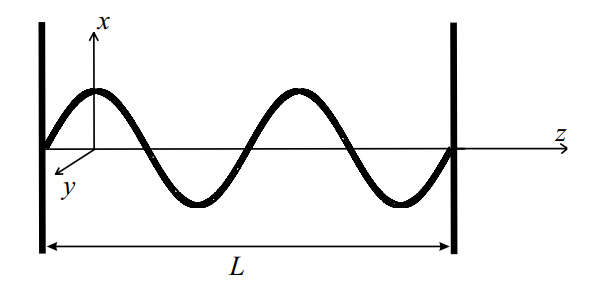
\includegraphics[scale=0.5]{em}
\end{figure}


Suppose that the field is a standing wave which vanishes on the boundary and is polarized in the $x$-direction. We also assume there is no source of radiation such as a charge or a current. The electric field then can be written as
\begin{align}
\mathbf{E}(\mathbf{r},t) = \mathbf{e}_xE_x(z,t)
\end{align}
where $\mathbf{e}_x$ is the polarization vector. The Maxwell's equations without source are
\begin{align}
\curl{\mathbf{E}} &= -\f{\p \mathbf{B}}{\p t}\\
\curl{\mathbf{B}} &= \mu_0\epsilon_0\f{\p \mathbf{E}}{\p t}\\
\div{\mathbf{E}} &= 0\\
\div{\mathbf{B}} &= 0.
\end{align}

A single-mode field satisfying Maxwell’s equations and the boundary conditions is given by
\begin{align}
E_x(z,t) = \lp \f{2\omega^2}{V\epsilon_0} \rp^{1/2} q(t)\sin(kz).
\end{align}
$\omega$ is the frequency, $k = \omega/c$ is the wavenumber. The allowed frequencies are
\begin{align}
\omega_m = c\f{m \pi}{L},\hspace{0.5cm}  =1,2,\dots
\end{align} 
$V$ is the effective volume of the cavity and $q(t)$ is the time-dependent factor having the dimension of length. The magnetic field, from the second Maxwell equation, is
\begin{align}
\mathbf{B}(\mathbf{r},t) = \mathbf{e}_yB_y(z,t)
\end{align}
where
\begin{align}
B_y(z,t) = \lp \f{\mu_0\epsilon_0}{k} \rp\lp \f{2\omega^2}{V\epsilon_0} \rp^{1/2}\dot{q}(t)\cos(kz).
\end{align}
It will become clear that $q(t)$ plays the role of canonical position, and $\dot{q}(t) = p(t)$ plays the role of canonical momentum. The classical field energy (or the Hamiltonian $\ham$) of this single-mode field is then given by
\begin{align}
\ham &= \f{1}{2}\int\,dV \lb \epsilon_0 \mathbf{E}^2(\mathbf{r},t) + \f{1}{\mu_0}\mathbf{B}^2(\mathbf{r},t) \rb\\
&= \f{1}{2}\int\,dV \lb \epsilon_0 E^2_x(z,t) + \f{1}{\mu_0}B_y^2(z,t) \rb
\end{align}
It turns out that (for $p(t) = \dot{q}(t)$), we have
\begin{align}
\boxed{\ham = \f{1}{2}\lp p^2 + \omega^2q^2 \rp}
\end{align} 
Now, we notice that we have the canonical variables $q$ and $p$. When we promote these variables to operators (so we can quantize the fields), these operators must satisfy the canonical commutation relation
\begin{align}
[\hat{q}, \hat{p}] = i\hbar \hat{\Id}.
\end{align}



We rewrite the fields and the Hamiltonian as operators:
\begin{align}
\hat{E}_x(z,t) &= \lp \f{2\omega^2}{V\epsilon_0} \rp^{1/2} \hat{q}(t)\sin(kz)\\
\hat{B}_y(z,t) &= \lp \f{\mu_0\epsilon_0}{k} \rp\lp \f{2\omega^2}{V\epsilon_0} \rp^{1/2}\hat{p}(t)\cos(kz).\\
\hat{\ham} &= \f{1}{2}\lp \hat{p}^2 + \omega^2\hat{q}^2 \rp.
\end{align}
The operators $\hat{q}$ and $\hat{p}$ correspond to observables because they are Hermitian. We can also introduce creation ($\hat{a}^\dagger$) and annihilation ($\hat{a}$) operators through combining $\hat{q}$ and $\hat{p}$:
\begin{align}
\hat{a} &= (2\hbar\omega)^{-1/2}(\omega\hat{q} + i\hat{p})\\
\hat{a}^\dagger &= (2\hbar\omega)^{-1/2}(\omega\hat{q} - i\hat{p})
\end{align}
It is easy to show that the electric and magnetic field operators then become
\begin{align}
\hat{E}_x(z,t) &= \mathcal{E}_0(\hat{a} + \hat{a}^\dagger)\sin(kz)\\
\hat{B}_y(z,t) &= \mathcal{B}_0\f{1}{i}(\hat{a} - \hat{a}^\dagger)\cos(kz)
\end{align}
where
\begin{align}
\mathcal{E}_0 = \sqrt{\f{\hbar\omega}{\epsilon_0 V}}, \hspace{0.5cm}
\mathcal{B}_0 = \lp\f{\mu_0}{k}\rp\sqrt{\f{\epsilon_0\hbar\omega^3}{V}}
\end{align}
represents respectively the electric and magnetic field ``per photon.'' We notice that
\begin{align}
[\hat{a}, \hat{a}^\dagger] = \hat{\Id}
\end{align}
so the Hamiltonian takes the form
\begin{align}
\boxed{\hat{\ham} = \hbar\omega\lp \hat{a}^\dagger\hat{a} + \f{1}{2} \rp}
\end{align}

Now, what is the time dependent of these new operators? For an arbitrary operator $\hat{O}$, Heisenberg equation reads
\begin{align}
\f{d\hat{O}}{dt} = \f{i}{\hbar}[\hat{H},\hat{O}].
\end{align}
For the annihilation operator, this becomes
\begin{align}
\f{d\hat{a}}{dt} = \f{i}{\hbar}\lb \hbar\omega\lp \hat{a}^\dagger\hat{a} + \f{1}{2} \rp, \hat{a} \rb = -i\omega \hat{a}.
\end{align}
Thus,
\begin{align}
\boxed{\hat{a}(t) = \hat{a}(0)e^{i\omega t}}
\end{align}
Similarly for the creation operator, we have
\begin{align}
\boxed{\hat{a}^\dagger(t) = \hat{a}^\dagger(0) e^{i\omega t}}
\end{align}

Now, let $\ket{n}$ denote an energy eigenstate of the single mode field corresponding to energy $E_n$, then 
\begin{align}
\hat{\ham}\ket{n} = \hbar\omega\lp \hat{a}^\dagger\hat{a} + \f{1}{2} \rp\ket{n} = E_n\ket{n}.
\end{align}
Applying the creation operator $\hat{a}^\dagger$ from the left we have
\begin{align}
\hbar\omega\lp \hat{a}^\dagger\hat{a}^\dagger\hat{a} + \f{1}{2}\hat{a}^\dagger \rp\ket{n} = E_n\hat{a}^\dagger\ket{n}.
\end{align}
Using the commutation relation, we can write 
\begin{align}
\hat{a}\hat{a}^\dagger = \hat{\Id} + \hat{a}^\dagger\hat{a}.
\end{align}
Thus,
\begin{align}
E_n\hat{a}^\dagger\ket{n} &= \hbar\omega\lp \hat{a}^\dagger[-\hat{\Id} + \hat{a}\hat{a}^\dagger] + \f{1}{2}\hat{a}^\dagger \rp\ket{n}\\
&= \hbar\omega\lp -\hat{a}^\dagger + \hat{a}^\dagger\hat{a}\hat{a}^\dagger + \f{1}{2}\hat{a}^\dagger \rp\ket{n}\\
&= \hbar\omega\lp -\hat{\Id} + \hat{a}^\dagger\hat{a} + \f{1}{2}  \rp\hat{a}^\dagger\ket{n}.
\end{align}
This says we have a new eigen-equation:
\begin{align}
(E_n + \hbar\omega) \hat{a}^\dagger\ket{n} = \hbar\omega\lp \hat{a}^\dagger\hat{a} + \f{1}{2} \rp\hat{a}^\dagger\ket{n}
\end{align}
or equivalently,
\begin{align}
\boxed{\hat{H}\lb\hat{a}^\dagger\ket{n}\rb = (E_n + \hbar\omega)\lb\hat{a}^\dagger\ket{n}\rb}
\end{align}
This is the eigenvalue problem for the eigenstate $\hat{a}^\dagger\ket{n}$ with the energy eigenvalue $E_n + \hbar\omega$. It is clear now why $\hat{a}^\dagger$ is called the creation operator: it creates a ``quantum'' energy $\hbar\omega$. On the other hand, we can also show that
\begin{align}
\boxed{\hat{H}\lb\hat{a}\ket{n}\rb = (E_n - \hbar\omega)\lb\hat{a}\ket{n}\rb} 
\end{align}
It is clear that the operator $\hat{a}$ annihilates a quantum of energy. Now, because for the least energetic eigenstate
\begin{align}
\hat{a}\ket{0} = 0,
\end{align}
the Hamiltonian of the annihilation of the least energetic eigenstate is 
\begin{align}
\hat{\ham}\lb \hat{a}\ket{0} \rb  = (E_0 - \hbar\omega)\lb \hat{a}\ket{0}\rb = 0.
\end{align}
Therefore,
\begin{align}
\hat{\ham}\ket{0} = \hbar\omega\lp \hat{a}^\dagger\hat{a} + \f{1}{2}\rp\ket{0} = \f{1}{2}\hbar\omega\ket{0} = E_0\ket{0}.
\end{align}
Or equivalently, the zero-point energy is 
\begin{align}
E_0 = \hbar\omega
\end{align}
and the energy eigenvalues $E_{n+1} = E_n + \hbar\omega$ are
\begin{align}
\boxed{E_n = \hbar\lp n + \f{1}{2}\rp}
\end{align}
Note that this is just like the energy levels for the harmonic oscillator in an infinite well. Now, we observe that
\begin{align}
\hat{\ham}\ket{n} = \hbar\omega\lp \hat{a}^\dagger\hat{a} + \f{1}{2}\rp \ket{n} = E_n\ket{n} = \hbar\omega\lp n + \f{1}{2} \rp\ket{n},
\end{align}
i.e.,
\begin{align}
\hat{a}^\dagger\hat{a}\ket{n} = n\ket{n}.
\end{align}
It makes sense to call $\hat{a}^\dagger\hat{a}$ the ``number operator'' $\hat{n}$, so that 
\begin{align}
\hat{n}\ket{n} = n\ket{n}.
\end{align}
Next, the eigenstates must be normalized according to $\braket{n} = 1$. For the state $\hat{a}\ket{n}$ we have
\begin{align}
\hat{a}\ket{n} = c_n\ket{n-1}.
\end{align}
Taking the inner product with itself we have
\begin{align}
\lp\bra{n}\hat{a}^\dagger\rp\lp\hat{a}\ket{n}\rp &= \bra{n}\hat{a}^\dagger\hat{a}\ket{n}\\
&= \bra{n}\hat{n}\ket{n}\\
&= n\braket{n}\\
&= \bra{n-1}c_n^*c_n\ket{n-1}.
\end{align}
This says $n = \abs{c_n}^2$. So we have
\begin{align}
\boxed{\hat{a}\ket{n} = \sqrt{n}\ket{n-1}}
\end{align}
Similarly, 
\begin{align}
\boxed{\hat{a}^\dagger\ket{n} = \sqrt{n+1}\ket{n+1}}
\end{align}
This says that $\ket{n}$ can be generated from the $\ket{0}$ state by applying the creation operator $\hat{a}^\dagger$ appropriately many times with the appropriate normalization:
\begin{align}
\boxed{\ket{n} = \f{{\lp\hat{a}^\dagger\rp}^n}{\sqrt{n!}}\ket{0}}
\end{align}


Next, because the eigenstates are orthonormal ($\braket{n'}{n} = \delta_{n'n}$ and $\braket{n}=1$) and form a complete set, i.e.,
\begin{align}
\sum^\infty_{n=0}\ket{n}\bra{n} = 1,
\end{align} 
the only non-vanishing matrix elements of the annihilation and creation operators are
\begin{align}
&\bra{n-1}\hat{a}\ket{n} = \sqrt{n}\braket{n-1} = \sqrt{n} \\
&\bra{n+1}\hat{a}^\dagger\ket{n} = \sqrt{n+1}\braket{n+1} = \sqrt{n+1}
\end{align}



\subsection{Quantum Fluctuations of a Single-mode Field}
Recall the electric field operator
\begin{align}
\hat{E}_x(z,t) &= \mathcal{E}_0(\hat{a} + \hat{a}^\dagger)\sin(kz).
\end{align}
The mean field is zero:
\begin{align}
\bra{n}\hat{E}_x(z,t)\ket{n} = \mathcal{E}_0\sin(kz)[\underbrace{\bra{n}\hat{a}\ket{n}}_{0} + \underbrace{\bra{n}\hat{a}^\dagger\ket{n}}_{0}] = 0
\end{align}
by orthonormality. However, the mean of the square of the field is not zero:
\begin{align}
\bra{n}\hat{E}^2_x(z,t)\ket{n} &= \mathcal{E}^2_0\sin^2(kz)\bra{n}{\lp\hat{a}^\dagger\rp}^2 + \hat{a}^2 + \hat{a}^\dagger\hat{a}+ \hat{a}\hat{a}^\dagger\ket{n}\\
&= \mathcal{E}^2_0\sin^2(kz)\bra{n} 2\hat{a}^\dagger\hat{a} + 1  \ket{n} \\
&= 2\mathcal{E}^2_0\sin^2(kz)\lp n + \f{1}{2}\rp.
\end{align}
So, the fluctuations in the field for the state $\ket{n}$ may be characterized by the variance
\begin{align}
\text{Var}[\hat{E}_x(z,t)] &= \text{E}[\hat{E}^2_x(z,t)] - \text{E}^2[\hat{E}_x(z,t)] \\ &= 2\mathcal{E}^2_0\sin^2(kz)\lp n + \f{1}{2}\rp.
\end{align}
And so the uncertainty of the field for the state $\ket{n}$ is
\begin{align}
\boxed{\sigma[\hat{E}_x(z,t)]= \sqrt{2\mathcal{E}_0}\sin(kz)\sqrt{n+ \f{1}{2}}}
\end{align}
Now, note that even at $n=0$, the field still has fluctuations. These are called ``vacuum fluctuations.'' Now the number states $\ket{n}$ are taken to represent a state of the field containing $n$ photons. Yet as we have seen, the average field is zero. This is all in accordance with the uncertainty principle because the number operator $\hat{n} = \hat{a}^\dagger\hat{a}$ does not commute with the electric field:
\begin{align}
[\hat{n}, \hat{E}_x] = \mathcal{E}_0 \sin(kz)(\hat{a}^\dagger - \hat{a}).
\end{align}
Thus $\hat{n}$ and $\hat{E}_x$ are complementary quantities for which their respective uncertainties obey the inequality
\begin{align}
\sigma[ n ]\cdot \sigma[ E_x ]\geq \f{1}{2}\mathcal{E}_0\abs{\sin(kz)}\abs{\langle \hat{a}^\dagger - \hat{a}\rangle}
\end{align}
This says that if the field is accurately known, then the number of photons in uncertain. 



\subsection{Quadrature Operators for a Single-mode Field}

When we explicitly include the time dependence of the electric field operator we have
\begin{align}
\hat{E}_x = \mathcal{E}_0 (\hat{a}e^{-\omega t} + \hat{a}^\dagger e^{i\omega t})\sin(kz)
\end{align}
where
\begin{align}
\hat{a}(0) \equiv \hat{a} \hspace{0.5cm} \hat{a}^\dagger(0) \equiv \hat{a}^\dagger.
\end{align}

Next, we define quadrature operators:
\begin{align}
&\hat{X}_1 = \f{1}{2}(\hat{a} + \hat{a}^\dagger)\\
&\hat{X}_2 = \f{1}{2i}(\hat{a} - \hat{a}^\dagger).
\end{align}
With these definitions, we rewrite the time-dependent electric field operator as
\begin{align}
\hat{E}_x(t) = 2\mathcal{E}_0\sin(kz)[\hat{X}_1 \cos(\omega t) + \hat{X}_2\sin(\omega t)].
\end{align}

We observe that $\hat{X}_1$ and $\hat{X}_2$ are associated with field amplitudes oscillating $\pi/2$ out of phase. Essentially, $\hat{X}_1$ and $\hat{X}_2$ are position and momentum operators, only scaled to be dimensionless. These operators satisfy the commutation relation
\begin{align}
[\hat{X}_1, \hat{X}_2] = \f{i}{2},
\end{align}
which one can easily check. Next, by definition we have
\begin{align}
\bra{n}\hat{X}_1\ket{n} = \bra{n}\hat{X}_2\ket{n} = 0.
\end{align}
However, 
\begin{align}
\bra{n}\hat{X}_1^2\ket{n} &= \f{1}{4}\bra{n} \hat{a}^2 + (\hat{a}^\dagger)^2 + \hat{a}^\dagger\hat{a} + \hat{a}\hat{a}^\dagger \ket{n}\\
&= \f{1}{4}\bra{n} 2\hat{a}^\dagger\hat{a} + 1 \ket{n}\\
&= \f{1}{4}(2n + 1).
\end{align}
Similarly, 
\begin{align}
\bra{n}\hat{X}_2^2\ket{n} = \f{1}{4}(2n + 1).
\end{align}
Thus for a number state, the uncertainties in both quadratures are the same and furthermore the vacuum state ($n = 0$) minimizes the uncertainty product since
\begin{align}
\text{Var}[\hat{X}_1] = \text{Var}[\hat{X}_2] = \f{1}{4}.
\end{align}

From this section, we learn that the quanta of the single-mode cavity field are the excitations of energy in discrete amounts of $\hbar\omega$. These quantas (or photons) are not localized particles but rather are spread out over the entire mode volume. 

















\subsection{Multimode Fields}

Now we generalize our results for the single-mode field to multi-mode fields. We again assume that there is no source of radiation. Let the vector potential $\mathbf{A}(\mathbf{r},t)$ be given such that
\begin{align}\label{gauge}
\div{\mathbf{A}(\mathbf{r},t)} = 0.
\end{align}
The vector potential gives the electric and magnetic fields by
\begin{align}\label{EB}
\mathbf{E}(\mathbf{r},t) &= -\f{\p \mathbf{A}(\mathbf{r},t)}{\p t}\\
\mathbf{B}(\mathbf{r},t) &= \curl{\mathbf{A}(\mathbf{r},t)}.
\end{align}
The vector potential satisfies the wave equation
\begin{align}\label{waves}
\laplacian{\mathbf{A}(\mathbf{r},t)} - \f{1}{c^2}\f{\p^2 \mathbf{A}(\mathbf{r},t)}{\p t^2} = 0.
\end{align}

We now assume free space is a cubic cavity with perfectly reflecting walls of length $L$. We assume that $L \to \infty$, i.e., $L$ is much larger than the wavelength of the field. This allows us to impose boundary conditions:
\begin{align}
&e^{ik_x x} = e^{ik_x(x+L)}\\
&e^{ik_y x} = e^{ik_y(y+L)}\\
&e^{ik_z x} = e^{ik_z(z+L)}.
\end{align}
It follows that
\begin{align}
&k_x = \lp \f{2\pi}{L} \rp m_x, \hspace{0.5cm} m_x = 0, \pm 1, \pm 2, \dots\\
&k_y = \lp \f{2\pi}{L} \rp m_y, \hspace{0.5cm} m_y = 0, \pm 1, \pm 2, \dots\\
&k_z = \lp \f{2\pi}{L} \rp m_z, \hspace{0.5cm} m_z = 0, \pm 1, \pm 2, \dots
\end{align}
The wave vector is then
\begin{align}
\mathbf{k} = \f{2\pi }{L}\begin{bmatrix}
m_x\\m_y\\m_z
\end{bmatrix}.
\end{align}
The magnitude of this vector is related to the frequency $\omega_k$ according to $k = \omega_k / c$. A set of integers $(m_x , m_y , m_z)$ specifies a normal mode of the field (apart from polarization), the number of modes being infinite but denumerable. The total number of modes in the intervals $\Delta m_x, \Delta m_y, \Delta m_z$ is
\begin{align}
\Delta m = \Delta m_x \Delta m_y \Delta m_z = 2\lp \f{L}{2\pi} \rp^3 \Delta k_x \Delta k_y \Delta k_z
\end{align}
where the factor of $2$ takes into account two independent modes of polarization. With the assumption that $L$ is very large compared to the wavelengths, this becomes
\begin{align}
dm = 2\lp \f{V}{8\pi^3} \rp d k_x d k_y d k_z.
\end{align}
In spherical coordinates, 
\begin{align}
\mathbf{k} = k(\sin\theta\cos\phi, \sin\theta\sin\phi, \cos\theta),
\end{align}
and 
\begin{align}
dm = 2\lp \f{V}{8\pi^3} \rp k^2 \, dk d\Omega
\end{align}
where
\begin{align}
d\Omega = \sin\theta \,d\theta d\phi.
\end{align}
With $k = \omega_k/c$,
\begin{align}
dm = 2\lp \f{V}{8\pi^3} \rp \f{\omega^2_k}{c^3} \, d\omega_k d\Omega.
\end{align}
Integrating over all solid angles gives $\int \,d\Omega = 4\pi$, so the number of modes in all directions from $k \to k + dk$ is 
\begin{align}
2\lp \f{V}{8\pi^3} \rp k^2 \cdot (4\pi) \, dk = V \f{k^2}{\pi^2}\,dk = V \rho_k \,dk
\end{align}
where $\rho_k = k^2/\pi^2$ and $\rho_k \,dk$ is the number of modes per unit volume. Integrating in the same fashion but with $\omega_k$ gives the number of modes in all directions from $\omega_k \to \omega_k + d\omega_k$:
\begin{align}
V \lp \f{\omega_k^2}{\pi^2 c^3} \rp\,d\omega_k = V \rho(\omega_k)\,d\omega_k
\end{align}
where now $\rho(\omega_k)$ is also the mode density. \\

The vector potential can be written as a superposition on plane waves in the form
\begin{align}
\mathbf{A}(\mathbf{r},t) = \sum_{\mathbf{k},s}\mathbf{e}_{\mathbf{k}s} \lb A_{\mathbf{k}s}(t)e^{i\mathbf{k}\cdot\mathbf{r}} + A_{\mathbf{k}s}^* e^{-i\mathbf{k}\cdot \mathbf{r}} \rb 
\end{align}
where $A_{\mathbf{k}s}$ is the complex amplitude of the field and $\mathbf{e}_{\mathbf{k}s}$ is a real polarization vector. The sum over $k$ simply means the sum over the set of integers $(m_x , m_y , m_z)$ and the sum over $s$ is the sum over the two independent polarizations. These polarizations must be orthogonal:
\begin{align}
\mathbf{e}_{\mathbf{k}s} \cdot \mathbf{e}_{\mathbf{k}s'} = 0
\end{align}
and the \textit{transversality} condition must be satisfied:
\begin{align}
\mathbf{k}\cdot\mathbf{e}_{\mathbf{k}s} = 0,
\end{align}
which is just says that the polarization is orthogonal to the propagation. The polarization vectors $\mathbf{e}_{\mathbf{k}1}$ and $\mathbf{e}_{\mathbf{k}2}$ form a right-handed system:
\begin{align}
\mathbf{e}_{\mathbf{k}1}\times \mathbf{e}_{\mathbf{k}2} = \f{\mathbf{k}}{\abs{\mathbf{k}}} = \mathbf{\kappa}.
\end{align}
In free space, we make the transition from ``discrete'' modes to a continuum of modes, thus the sum becomes an integral:
\begin{align}
\sum_{\mathbf{k}} \to \f{V}{\pi^2}\int k^2\,dk.
\end{align}
From \eqref{gauge} and \eqref{waves} and $\omega_k = kc$, we get
\begin{align}
\f{d^2 A_{\mathbf{k}s}}{dt^2} + \omega_k^2 A_{\mathbf{k}s} =0. 
\end{align}
The solution to this is of course
\begin{align}
A_{\mathbf{k}s}(t) = A_{\mathbf{k}s}(0)e^{-i\omega_k t} = A_{\mathbf{k}s}e^{-i\omega_k t}.
\end{align}
From this and \eqref{EB} we can derive the electric and magnetic fields:
\begin{align}
&\mathbf{E}(\mathbf{r},t) = i\sum_{\mathbf{k},s} \omega_k \mathbf{e}_{\mathbf{k}s} \lb A_{\mathbf{k}s}e^{i(\mathbf{k}\cdot\mathbf{r} - \omega_k t)} - A_{\mathbf{k}s}^* e^{-i(\mathbf{k}\cdot\mathbf{r} - \omega_k t)}\rb\\
&\mathbf{B}(\mathbf{r},t) = \f{i}{c}\sum_{\mathbf{k},s} \omega_k (\mathbf{\kappa} \times \hat{\mathbf{e}}_{\mathbf{k}s}) \lb A_{\mathbf{k}s}e^{i(\mathbf{k}\cdot\mathbf{r} - \omega_k t)} - A_{\mathbf{k}s}^* e^{-i(\mathbf{k}\cdot\mathbf{r} - \omega_k t)}\rb.
\end{align}
The electromagnetic Hamiltonian is given by
\begin{align}
\ham = \f{1}{2}\int_V \lp \epsilon_0 \mathbf{E}\cdot \mathbf{E} + \f{1}{\mu_0} \mathbf{B}\cdot\mathbf{B} \rp\,dV.
\end{align}
The periodic boundary conditions result in
\begin{align}
\int_0^L e^{\pm i k_x x}\,dx = \begin{cases}
L,\hspace{0.5cm} k_x = 0\\
0,\hspace{0.5cm} k_x \neq 0
\end{cases}
\end{align}
same for $y$ and $z$. Collectively we write this as
\begin{align}
\int_V e^{\pm i(\mathbf{k} - \mathbf{k}')\cdot\mathbf{r}} \, dV = \delta_{\mathbf{k}\mathbf{k}'}V.
\end{align}
So the contribution to the Hamiltonian from the electric field is
\begin{align}
\f{1}{2}\int_V \epsilon_0 \mathbf{E}\cdot\mathbf{E}\,dV = &\epsilon_0 V \sum_{\mathbf{k}s}\omega_k^2 A_{\mathbf{k}s}(t)A^*_{\mathbf{k}s}(t) \\
& - \underbrace{\f{1}{2}\epsilon_0 V\sum_{\mathbf{k}ss'}\omega^2_k \mathbf{e}_{\mathbf{k}s}\cdot \mathbf{e}_{-\mathbf{k}s'}\lb A_{\mathbf{k}s}(t)A_{\mathbf{k}s'}(t) + A^*_{\mathbf{k}s}(t)A^*_{-\mathbf{k}s'}(t) \rb}_R.
\end{align}
To obtain the magnetic contribution we use the identity
\begin{align}
(\mathbf{A}\times \mathbf{B})\cdot (\mathbf{C}\times \mathbf{D}) = (\mathbf{A}\cdot\mathbf{C})(\mathbf{B}\cdot \mathbf{D}) - (\mathbf{A}\cdot\mathbf{D})(\mathbf{B}\cdot\mathbf{C}).
\end{align}
This gives
\begin{align}
(\mathbf{\kappa}\times \mathbf{e}_{\mathbf{k}s})\cdot(\mathbf{\kappa}\times \mathbf{e}_{\mathbf{k}s'}) &= \delta_{ss'}\\
(\mathbf{\kappa}\times \mathbf{e}_{\mathbf{k}s})\cdot(-\mathbf{\kappa}\times \mathbf{e}_{-\mathbf{k}s'}) &= -\mathbf{e}_{\mathbf{k}s}\cdot \mathbf{e}_{-\mathbf{k}s'}.
\end{align}
With this we get the contribution from the magnetic field
\begin{align}
\f{1}{2}\int_V \f{1}{\mu_0}\mathbf{B}\cdot\mathbf{B}\,dV = &\epsilon_0 V \sum_{\mathbf{k}s}\omega^2_k A_{\mathbf{k}s}(t)A^*_{\mathbf{k}s}(t) + R.
\end{align}
Thus the Hamiltonian is
\begin{align}
\ham &= 2\epsilon_0 V \sum_{\mathbf{k}s} \omega^2_k A_{\mathbf{k}s}(t)A^*_{\mathbf{k}s}(t)\\
&= 2\epsilon_0 V \sum_{\mathbf{k}s} \omega^2_k A_{\mathbf{k}s}(0)e^{-i\omega_k t}A^*_{\mathbf{k}s}(0)e^{i\omega_k t}\\
&= 2\epsilon_0 V \sum_{\mathbf{k}s} \omega^2_k A_{\mathbf{k}s}A^*_{\mathbf{k}s}.
\end{align}
To quantize the field, the canonical variables $q_{\mathbf{k}s}$ and $p_{\mathbf{k}s}$ must be introduced:
\begin{align}
A_{\mathbf{k}s} &= \f{1}{2\omega_k \sqrt{\epsilon_0 V}}[\omega_k q_{\mathbf{k}s} + ip_{\mathbf{k}s}]\\
A^*_{\mathbf{k}s} &= \f{1}{2\omega_k \sqrt{\epsilon_0 V}}[\omega_k q_{\mathbf{k}s} - ip_{\mathbf{k}s}]
\end{align}
such that when we can re-write the Hamiltonian as
\begin{align}
\ham = \f{1}{2}\sum_{\mathbf{k}s} \lp p^2_{\mathbf{k}s} + \omega_k^2q_{\mathbf{k}s}^2\rp.
\end{align}

To quantize the field, we promote these canonical variables to operators:
\begin{align}
\boxed{\hat{\ham} = \f{1}{2}\sum_{\mathbf{k}s} \lp \hat{p}^2_{\mathbf{k}s} + \omega_k^2\hat{q}_{\mathbf{k}s}^2\rp}
\end{align}
where 
\begin{align}
\lb\hat{q}_{\mathbf{k}s}, \hat{q}_{\mathbf{k}'s'}\rb &= 0 = \lb\hat{p}_{\mathbf{k}s}, \hat{p}_{\mathbf{k}'s'}\rb \\
\lb\hat{q}_{\mathbf{k}s}, \hat{p}_{\mathbf{k}'s'}\rb &= i\hbar\delta_{\mathbf{kk}'}\delta_{ss'}.
\end{align}
The annihilation and creation operators are defined in a similar fashion as in the case of a single-mode field:
\begin{align}
\hat{a}_{\mathbf{k}s} &= (2\hbar\omega_k)^{-1/2}(\omega_k \hat{q}_{\mathbf{k}s} + i\hat{p}_{\mathbf{k}s})\\
\hat{a}^\dagger_{\mathbf{k}s} &= (2\hbar\omega_k)^{-1/2}(\omega_k \hat{q}_{\mathbf{k}s} - i\hat{p}_{\mathbf{k}s})
\end{align}
which satisfy
\begin{align}
\lb\hat{a}_{\mathbf{k}s}, \hat{a}_{\mathbf{k}'s'}\rb &= 0 = \lb\hat{a}^\dagger_{\mathbf{k}s}, \hat{a}^\dagger_{\mathbf{k}'s'}\rb\\
\lb \hat{a}_{\mathbf{k}s}, \hat{a}^\dagger_{\mathbf{k}'s'}  \rb &= \delta_{\mathbf{kk}'}\delta_{ss'}.
\end{align}
Finally, we define a similar operator for the mode $\mathbf{k}s$ as the ``number'' operator before
\begin{align}
\hat{n}_{\mathbf{k}s} = \hat{a}^\dagger_{\mathbf{k}s} \hat{a}_{\mathbf{k}s}.
\end{align}
With these, the Hamiltonian (operator) can be written as
\begin{align}
\hat{\ham} = \sum_{\mathbf{k}s}\hbar\omega_k \lp \hat{a}_{\mathbf{k}s}^\dagger\hat{a}_{\mathbf{k}s} + \f{1}{2} \rp = \sum_{\mathbf{k}s} \omega_k \lp \hat{n}_{\mathbf{k}s} +\f{1}{2} \rp.
\end{align}
For simplicity, we associate a $j^\text{th}$ mode with $\mathbf{k}_js_j$. We let
\begin{align}
\hat{a}_{\mathbf{k}_j s_j} &\equiv \hat{a}_j\\
\hat{a}^\dagger_{\mathbb{k}_j s_j} &\equiv \hat{a}^\dagger_j\\
\hat{n}_{\mathbf{k}_j s_j} &\equiv \hat{n}_j.
\end{align}
Now we can write the Hamiltonian as
\begin{align}
\boxed{\hat{\ham} = \sum_j \hbar\omega_j \lp \hat{n}_j + \f{1}{2} \rp}
\end{align}

A multimode photon number state is a (tensor) product of the number states $\ket{n_{\mathbf{k}s}} \equiv \ket{n_j}$ of all the modes which we write as
\begin{align}
\ket{n_1}\ket{n_2}\ket{n_3}\dots \equiv \ket{n_1n_2n_3\dots} = \ket{\{ n_j \}}.
\end{align}
This is an eigenstate of the Hamiltonian:
\begin{align}
\hat{\ham}\ket{\{ n_j \}} = E\ket{\{ n_j \}}.
\end{align}
We can show that energy eigenvalue is
\begin{align}
\boxed{E = \sum_j \hbar\omega_j \lp n_j + \f{1}{2} \rp}
\end{align}
Because the Hamiltonian is Hermitian (as always) the eigenstates are orthogonal:
\begin{align}
\bra{n_1n_2n_3\dots}\ket{n'_1n'_2n'_3\dots} = \delta_{n_1n'_1}\delta_{n_2n'_2}\delta_{n_3n'_3}\dots
\end{align}
The actions of the annihilation and creation operator are as expected and similar to what we have seen before:
\begin{align}
&\boxed{\textbf{Annihilation: } \hat{a}_j \ket{n_1,n_2,\dots,n_j,\dots} = \sqrt{n_j}\ket{n_1,n_2,\dots,n_j - 1,\dots}}\\
&\boxed{\textbf{Creation: } \hat{a}^\dagger_j \ket{n_1,n_2,\dots,n_j,\dots} = \sqrt{n_j + 1}\ket{n_1,n_2,\dots,n_j + 1,\dots}}
\end{align}


The vacuum multimode is denoted
\begin{align}
\ket{\{ 0 \}} = \ket{0_10_20_3\dots 0_j\dots}
\end{align}
for which
\begin{align}
\hat{a}_j \ket{\{ 0 \}} = 0 \hspace{0.5cm} \text{for all }j.
\end{align}
Once again, like in the single-mode case, a multimode number state can be generated by applying the creation operator. Any number state can be written as some creation operator applied to the multimode vacuum:
\begin{align}
\ket{\{ n_j \}} = \prod_{j} \f{(\hat{a}^\dagger_{j})^{n_j}}{\sqrt{n_j !}}\ket{\{ 0 \}}.
\end{align}

Now, we notice that the creation/annihilation operators $\hat{a}_{\mathbf{k}s}$/$\hat{a}^\dagger_{\mathbf{k}s}$ are very much like the vector potential amplitude $A_{\mathbf{k}s}$. Indeed, upon quantization of the field, the amplitudes can be promoted to operators as well:
\begin{align}
\hat{A}_{\mathbf{k}s} = \lp \f{\hbar}{2\omega_k \epsilon_0 V} \rp^{\f{1}{2}}\hat{a}_{\mathbf{k}s}.
\end{align}
With this, we are able to rewrite the vector potential, electric, and magnetic fields in terms of the creation and annihilation operators:
\begin{align}
&\hat{\mathbf{A}}(\mathbf{r},t) = \sum_{\mathbf{k}s}\lp\f{\hbar}{2\omega_k \epsilon_0 V}\rp^{\f{1}{2}} \mathbf{e}_{\mathbf{k}s} \lb \hat{a}_{\mathbf{k}s}e^{i(\mathbf{k}\cdot\mathbf{r} - \omega_k t)}
+ \hat{a}^\dagger_{\mathbf{k}s}e^{-i(\mathbf{k}\cdot\mathbf{r} - \omega_k t)}  \rb\\
&\hat{\mathbf{E}}(\mathbf{r},t) = i\sum_{\mathbf{k}s}\lp\f{\hbar\omega_k}{2\epsilon_0 V}\rp^{\f{1}{2}} \mathbf{e}_{\mathbf{k}s} \lb \hat{a}_{\mathbf{k}s}e^{i(\mathbf{k}\cdot\mathbf{r} - \omega_k t)}
- \hat{a}^\dagger_{\mathbf{k}s}e^{-i(\mathbf{k}\cdot\mathbf{r} - \omega_k t)}  \rb\\
&\hat{\mathbf{B}}(\mathbf{r},t) = \f{i}{c}\sum_{\mathbf{k}s} (\mathbf{\kappa} \times \mathbf{e}_{\mathbf{k}s})\lp\f{\hbar\omega_k}{2 \epsilon_0 V}\rp^{\f{1}{2}} \mathbf{e}_{\mathbf{k}s} \lb \hat{a}_{\mathbf{k}s}e^{i(\mathbf{k}\cdot\mathbf{r} - \omega_k t)}
- \hat{a}^\dagger_{\mathbf{k}s}e^{-i(\mathbf{k}\cdot\mathbf{r} - \omega_k t)}  \rb.
\end{align}



The annihilation and creation operators are to be understood as Heisenberg picture operators evaluated at $t=0$. The time-dependent annihilation operator for a free field is given by  
\begin{align}
\hat{a}_{\mathbf{k}s}(t) = \hat{a}_{\mathbf{k}s}(0)e^{-i\omega_k t}.
\end{align}
With this the electric field can be written as
\begin{align}
\hat{\mathbf{E}}(\mathbf{r},t) = i\sum_{\mathbf{k}s}\lp \f{\hbar\omega_k}{2\epsilon_0 V} \rp^{\f{1}{2}} \mathbf{e}_{\mathbf{k}s}   \lb \hat{a}_{\mathbf{k}s}(t)e^{i\mathbf{k}\cdot\mathbf{r}} - \hat{a}^\dagger_{\mathbf{k}s}(t)e^{-i\mathbf{k}\cdot\mathbf{r}} \rb.
\end{align}
where the $e^{\pm i \omega_k t}$ term is absorbed into the operator. Alternatively, the field can be written in a different form:
\begin{align}
\hat{\mathbf{E}}(\mathbf{r},t) = \hat{\mathbf{E}}^{(+)}(\mathbf{r},t) + \hat{\mathbf{E}}^{(-)}(\mathbf{r},t)
\end{align}
where
\begin{align}
\hat{\mathbf{E}}^{(+)}(\mathbf{r},t) = i\sum_{\mathbf{k}s}\lp \f{\hbar\omega_k}{2\epsilon_0 V} \rp^{\f{1}{2}}\mathbf{e}_{\mathbf{k}s}\hat{a}_{\mathbf{k}s}(t)e^{ i\mathbf{k}\cdot\mathbf{r}}.
\end{align}
Of course,
\begin{align}
\hat{\mathbf{E}}^{(+)}(\mathbf{r},t) = \lb \hat{\mathbf{E}}^{(-)}(\mathbf{r},t) \rb^\dagger.
\end{align}

Similar expressions can be obtained for the magnetic field. However, because the magnetic field is ``weaker'' than the electric field by a factor of $1/c$, we generally neglect the magnetic field in most matter-field interactions (as most interactions are through the electric dipole). $\hat{\mathbf{E}}^{(+)}(\mathbf{r},t)$ is called the \textit{positive frequency part} of the field as it contained all terms oscillate as $e^{-i\omega t}$ for $\omega > 0$. The opposite is for $\hat{\mathbf{E}}^{(-)}(\mathbf{r},t)$. We notice that $\hat{\mathbf{E}}^{(+)}(\mathbf{r},t)$ is a collective annihilation operator while the latter is a collective creation operator. \\

The last observation we make is the following. For a single-mode plane wave field the electric field is
\begin{align}
\hat{E}(\mathbf{r},t) = i\lp \f{\hbar\omega_k}{2\epsilon_0 V} \rp^{\f{1}{2}}\mathbf{e}_x\lb \hat{a} e^{i\mathbf{k}\cdot\mathbf{r} - i\omega t} - \hat{a}^\dagger e^{-i\mathbf{k}\cdot\mathbf{r} + i\omega t} \rb.
\end{align}
In most of quantum optics, the spatial variation of the field over the dimensions of the atomic system may be negligible, i.e., the length characteristic of the size of the atom is often much smaller than a typical wavelength:
\begin{align}
\f{\lambda}{2\pi} = \f{1}{\abs{k}} \gg \abs{\mathbf{r}_\text{atom}}.
\end{align}
With this, we can make an approximation:
\begin{align}
e^{\pm i\mathbf{k}\cdot\mathbf{r}} \approx 1 \pm i\mathbf{k}\cdot\mathbf{r}
\end{align}
which says we replace the exponential by unity for $\abs{\mathbf{r}}$ is negligible. Under this approximation, 
\begin{align}\label{dipoleE}
\boxed{\hat{\mathbf{E}}(\mathbf{r},t)  \approx \hat{\mathbf{E}}(t) = i \lp \f{\hbar\omega_k}{2\epsilon_0 V} \rp^{\f{1}{2}}\mathbf{e}_x \lb \hat{a}e^{-i\omega t} - \hat{a}^\dagger e^{i\omega t} \rb}
\end{align}
This is called the \textbf{``dipole'' approximation}. 




%\newpage
%
%\section{Coherent States}

\newpage

\section{Emission and Absorption of Radiation by Atoms}

\subsection{Atom-field interactions}
Suppose we have an atom in no external field. The Hamiltonian of an electron bound to this atom is given by
\begin{align}
\hat{\ham}_0 = \f{1}{2m}\hat{\mathbf{P}}^2 + V(r)
\end{align}
where $V(r)$ is the Coulomb interaction between the electron and nucleus and $r = \abs{\mathbf{r}}$ is the distance to the core. In the configuration space representation, 
\begin{align}
&\hat{\mathbf{P}} = -i \hbar \nabla\\
&\hat{\mathbf{r}}\ket{\mathbf{r}} = \mathbf{r}\ket{\mathbf{r}}.
\end{align}
The wave functions are given by
\begin{align}
\psi(\mathbf{r}) = \bra{\mathbf{r}}\ket{\psi}.
\end{align}
We assume that the energy eigenstates $\ket{k}$ of $\hat{\ham}_0$ satisfy the time-independent Schr\"{o}dinger equation:
\begin{align}
\hat{\ham}_0 \ket{\psi}_k^{(0)}(\mathbf{r}) = E_k \psi_k^{(0)}(\mathbf{r}) 
\end{align}
where 
\begin{align}
\bra{\mathbf{r}}\ket{k} = \psi_k^{(0)}(\mathbf{r})
\end{align}
are known. In the presence of external fields the Hamiltonian is modified to
\begin{align}
\hat{\ham}(\mathbf{r},t) = \f{1}{2m}\lb \hat{\mathbf{P}} + e\mathbf{A}(\mathbf{r} , t) \rb^2 - e\Phi(\mathbf{r},t) + V(r)
\end{align}
where $\mathbf{A}(\mathbf{r},t)$ and $\Phi(\mathbf{r},t)$ are the vector and scalar potentials, respectively, $-e$ is the electron charge. The electric and magnetic fields are given by
\begin{align}
&\mathbf{E}(\mathbf{r},t) = -\grad{\Phi(\mathbf{r},t)} - \f{\p \mathbf{A}(\mathbf{r},t)}{\p t}\\
&\mathbf{B}(\mathbf{r},t) = \curl{\mathbf{A}(\mathbf{r},t)}
\end{align}
which we can easily show to be invariant under the following gauge transformations
\begin{align}\label{gaug}
&\Phi'(\mathbf{r},t) = \Phi(\mathbf{r},t) - \f{\p \chi(\mathbf{r},t)}{\p t}\\
&\mathbf{A}'(\mathbf{r},t) = \mathbf{A}(\mathbf{r},t) + \grad{\chi(\mathbf{r},t)}.
\end{align}
The time-dependent Schr\"{o}dinger equation is
\begin{align}
\hat{\ham}(\mathbf{r},t)\psi(\mathbf{r},t) = i\hbar\f{\p \psi(\mathbf{r},t)}{\p t}.
\end{align}
To eventually simplify the form of the atom-field interaction, we define a unitary operator $\hat{R}$ such that
\begin{align}
\psi'(\mathbf{r},t) = \hat{R}\psi(\mathbf{r},t)
\end{align}
where
\begin{align}
\hat{\ham}' \psi'  = i\hbar \f{\p \psi'}{\p t}.
\end{align}
We can show that the new Hamiltonian relates to the old Hamiltonian as 
\begin{align}
\hat{\ham}' = \hat{R}\hat{\ham}\hat{R}^\dagger + i\hbar \f{\p \hat{R}}{\p t}\hat{R}^\dagger.
\end{align}
Our goal is to choose 
\begin{align}
\hat{R} = e^{-ie\chi(\mathbf{r},t)/\hbar},
\end{align}
so that with $\hat{\mathbf{P}}^2 = -i\hbar \nabla$:
\begin{align}
\hat{\ham}' =\f{1}{2m}\lb \hat{\mathbf{P}}^2 + e\mathbf{A}' \rb^2 - e\Phi' + V(r),
\end{align}
where the new vector and scalar potentials $\mathbf{A}'$ and $\Phi'$ depend on the gauge field $\chi$ as \eqref{gaug}. This form of the Hamiltonian is not desirable because of the interaction terms $\hat{\mathbf{P}} \cdot \mathbf{A}$ and $\mathbf{A}^2$. To remedy this, we can first make a definite choice of gauge, namely the Coulomb gauge, for which $\Phi = 0$ and $\div{\mathbf{A}} = 0$. Now with $\mathbf{A'} = \mathbf{A} + \grad{\chi}$ and $\Phi' = \Phi - \p \chi / \p t = - \p \chi / \p t$, the new Hamiltonian has the form
\begin{align}\label{newHam}
\hat{\ham}' = \f{1}{2m}\lb \hat{\mathbf{P}} + e\lp\mathbf{A} + \grad{\chi}\rp \rb^2 + e\f{\p \chi}{\p t} +V(r).
\end{align}
The vector potential $\mathbf{A}$ for no sources near the atom satisfies the wave equation
\begin{align}
\laplacian{\mathbf{A}} - \f{1}{c^2}\f{\p^2 \mathbf{A}}{\p t^2} = 0,
\end{align}
whose solution is simply a wave propagating wave
\begin{align}
\mathbf{A} = \mathbf{A}_0 e^{i(\mathbf{k}\cdot\mathbf{x} - \omega t)} + c.c.
\end{align}
where $\abs{\mathbf{k}} = 2\pi/\lambda$ is the wave vector of the radiation. For $\abs{\mathbf{r}}$ a typical atomic length ($10^{-10}$ m) and $\lambda$ of typical optical wavelengths ($10^{-7}$ m), the product $\mathbf{k}\cdot\mathbf{r} \ll 1$ so that over the extend of the atom $\mathbf{A}$ can be taken to be uniform, i.e.,
\begin{align}
\mathbf{A}(\mathbf{r},t) \approx \mathbf{A}(t).
\end{align} 
This is very much like the idea we discussed before regarding the electric field $\mathbf{E}$ in the quantization of the EM field. This is also called the \textbf{dipole approximation}. Now, the Hamiltonian in \eqref{newHam} has coupled terms, and we would like to remove $\nabla \chi$ from the coupling between itself and $\mathbf{A}$ and between $\mathbf{A}$ and $\hat{\mathbf{P}}$. One very good way to do this is finding $\chi$ such that
\begin{align}
\nabla \chi = - \mathbf{A}(\mathbf{r},t) \approx \mathbf{A}(t).
\end{align}
Such a $\chi(\mathbf{r},t)$ is
\begin{align}
\chi(\mathbf{r},t) = - \mathbf{A}(t)\cdot \mathbf{r}.
\end{align}
With this choice, we have (since $\nabla \mathbf{r} = \mathbf{1}$)
\begin{align}
&\nabla \chi(\mathbf{r},t) = -\mathbf{A}(t)\\
&\f{\p \chi}{\p t}(\mathbf{r},t) = -\mathbf{r}\cdot \f{\p \mathbf{A}(t)}{\p t} = -\mathbf{r}\cdot \mathbf{E}(t).
\end{align}
The new Hamiltonian is now ``decoupled":
\begin{align}
\boxed{\hat{\ham}' = \underbrace{\f{1}{2m}\hat{\mathbf{P}}^2 + V(r)}_{\text{field-free}} \underbrace{-e\mathbf{r}\cdot \mathbf{E}(t)}_{\text{dipole int.}}}
\end{align}
This new Hamiltonian contains only one interaction term (within the dipole approximation) as opposed to two terms as before. $-e\mathbf{r}$ is called the \textbf{dipole moment}, denoted $\mathbf{d}$. We can of course promote it to an operator, so that the Hamiltonian in the presence of an external field can be written as
\begin{align}
\boxed{\hat{\ham} = \hat{\ham}_0 - \hat{\mathbf{d}}\cdot\mathbf{E}(t)}
\end{align}
where $\hat{\ham}_0 = \hat{\mathbf{P}}^2/2m + V(r)$ is of course the field-free Hamiltonian. 



\subsection{Interaction of an atom with a classical field}

So far we have not specified whether the interacting field is classical or quantum mechanical. The derivation we just looked at is valid for both classical and quantum fields. However, we will eventually show that the atom behaves differently in each case. 

Let us first look at the the atom-field interaction with a classical field. Suppose the field is given by
\begin{align}
\mathbf{E}(t) = \mathbf{E}_0 \cos(\omega t)
\end{align}
where the dipole approximation $\mathbf{k}\cdot\mathbf{r} \ll 1$ has already been made (so that the field is uniform over the atom). Suppose that $\omega$ is the frequency of the radiation, and the field is abruptly turned on at $t = 0$. Assume that the initial state of the atom is $\ket{i}$ where
\begin{align}
\hat{\ham}_0 \ket{i} = E_i\ket{i}. 
\end{align}
For time $t > 0$, the state vector $\ket{\psi}(t)$ is a linear combination of all uncoupled states $\ket{k}$:
\begin{align}\label{exp}
\ket{\psi(t)} = \sum_k C_k(t) e^{-iE_k t/\hbar}\ket{k}
\end{align}
where
\begin{align}
\sum_k \abs{C_k(t)}^2= 1.
\end{align}
The time-dependent Schro\"{o}dinger equation is
\begin{align}
i\hbar \f{\p \ket{\psi(t)}}{\p t} = \lp \hat{\ham}_0 + \hat{\ham}^{(I)} \rp\ket{\psi(t)}
\end{align}
where
\begin{align}
\hat{\ham}^{(I)} = -\hat{\mathbf{d}}\cdot\mathbf{E}(t).
\end{align}
Substituting the expansion \eqref{exp} into the time-dependent SE, them multiplying from the left by $\bra{l}e^{-E_l t/\hbar}$ gives
\begin{align}
i\hbar \bra{l}e^{-E_l t/\hbar} \f{\p}{\p t}\sum_k C_k(t) e^{-iE_k t/\hbar}\ket{k} = \bra{l}e^{-i E_l t/\hbar} \lp \hat{\ham}_0 + \hat{\ham}^{(I)} \rp \sum_k C_k(t) e^{-iE_k t/\hbar}\ket{k}.
\end{align}
This simplifies to 
\begin{align}
\dot{C}_l(t) - \f{i}{\hbar}\sum_k C_k(t)\bra{l}\hat{\ham}^{(I)}\ket{k} e^{-i (E_l - E_k)t\hbar}.
\end{align}
Defining
\begin{align}
\omega_l = \f{E_l - E_K}{\hbar}
\end{align}
as the transition frequencies between levels $l$ and $k$ gives a set of couple-first-order differential equations for the amplitudes
\begin{align}\label{dif}
\dot{C}_l(t)=  - \f{i}{\hbar}\sum_k C_k(t)\bra{l}\hat{\ham}^{(I)}\ket{k} e^{-i\omega_l t}.
\end{align}
The initial condition is $C_i(0) = 1$: $\ket{i}$ is the only state initially populated. As time goes forward, the population in $\ket{i}$ will decrease and move to some unpopulated $\ket{f}$. The probability of the transition $i \to f$ is given by
\begin{align}
P_{i\to f}(t) = C^*(f)C_f(t) = \abs{C_f(t)}^2. 
\end{align}
For simple cases, these probabilities can be solved analytically or even numerically for more complex cases. However, for the ``weak'' field where $\abs{\bra{f}\hat{\mathbf{d}\cdot\mathbf{E}_0}\ket{i}}$ is small, we can use the time-dependent perturbation theory to approach the problem. For bookkeeping purposes we shall write the interaction Hamiltonian as $\lambda \hat{\ham}^{(1)}$ where $0 \leq \lambda \leq 1$. (At the end of the calculations we often take $\lambda \to 1$.) We then expand the probability amplitude for, say, the state $\ket{l}$ in the power series
\begin{align}
C_l(t) = \sum_{n = 0}^\infty \lambda^n C_l^{(n)}(t).
\end{align} 
Inserting this expansion into \eqref{dif} and equating the like powers of $\lambda$ we obtain up to second order
\begin{align}
&\dot{C}_l^{(0)} = 0\\
&\dot{C}_l^{(1)} = -\f{i}{\hbar}\sum_k C_k^{(0)}(t)\ham^{(I)}_{lk}(t)e^{i\omega_{lk}t}\\
&\dot{C}_l^{(2)} = -\f{i}{\hbar}\sum_k C_k^{(1)}(t)\ham^{(I)}_{lk}(t)e^{i\omega_{lk}t}
\end{align}
where
\begin{align}
\ham^{(I)}_{lk}(t) = \bra{l}\hat{\ham}^{(I)}(t)\ket{k} = \bra{l}- \hat{\mathbf{d}} \cdot\mathbf{E}(t)\ket{k}.
\end{align}
We observe the pattern relating the $n^{th}$ order to the $n+1^{th}$ order:
\begin{align}
\dot{C}_l^{(n+1)} = -\f{i}{\hbar}\sum_k C_k^{(n)}(t)\ham^{(I)}_{lk}(t)e^{i\omega_{lk}t}.
\end{align}
The essential assumption underlying the perturbation-theory approach is that the driving field is so weak that the atomic populations change very little. That is, if $C_i(0) = 1$ and $C_f(0) = 0$ then for $t > 0$, a good approximation is $C_i(t) \approx 1$ and $C_f(t) \ll 1$. Thus, for the expression of $\dot{C}^{(1)}_l$ the only surviving term is for the state $k$ to be the initial state $i$. This gives
\begin{align}
\dot{C}_f^{(1)}(t) = -\f{i}{\hbar} C_i^{(0)}(t)\ham^{(I)}_{fi}(t)e^{i\omega_{fi}t}.
\end{align}   
Integrating this gives
\begin{align}\label{c1}
{C}_f^{(1)}(t) = -\f{i}{\hbar}\int_0^t C_i^{(0)}(t')\ham^{(I)}_{fi}(t')e^{i\omega_{fi}t'}\,dt'.
\end{align}
Following a similar line of reasoning we get for $\dot{C}_l^{(2)}$
\begin{align}
\dot{C}_l^{(2)}(t) &= -\f{i}{\hbar}\sum_l \int_0^t C_l^{(1)}(t')\ham^{(I)}_{fl}(t')e^{i\omega_{fl}t'}\,dt'.
\end{align}
Now replacing $C_l^{(1)}$ with \eqref{c1} we get
\begin{align}\label{c2}
{C}_l^{(2)}(t) &= -\f{i}{\hbar}\sum_l \int_0^t 
\lp -\f{i}{\hbar}\int_0^{t'} C_i^{(0)}(t'')\ham^{(I)}_{fi}(t'')e^{i\omega_{fi}t''}\,dt''  \rp
\ham^{(I)}_{fl}(t')e^{i\omega_{fl}t'}\,dt'\\
&= \lp \f{-i}{\hbar} \rp^2 \sum_l \int_0^t\,dt' \int_0^{t'}\,dt'' \lp \ham^{(I)}_{fl}(t')e^{i\omega_{fl}t'}\rp \ham^{(I)}_{fi}(t'')e^{i\omega_{fi}t''} 
\end{align}
We see that while \eqref{c1} gives the transition probability amplitude from $\ket{i}\to \ket{f}$, \eqref{c2} gives the transition probability amplitude from $\ket{i} \to \ket{\{ l \}} \to \ket{f}$. The total transition probability from $\ket{i}$ to $\ket{f}$ is then the square of the sum of the amplitudes:
\begin{align}
P_{i\to f}(t)  = \abs{ \sum_{n=0}^\infty C^{(n)}_f(t)}^2.
\end{align}


The dipole moment operator $\hat{\mathbf{d}} = -e\mathbf{r}$ has non-vanishing matrix elements only between states of opposite parity. Thus the first-order correction to the amplitude of the initial state (where $f=i$) vanishes:
\begin{align}
{C}_i^{(1)}(t) = -\f{i}{\hbar}\int_0^t C_i^{(0)}(t')\ham^{(I)}_{ii}(t')e^{i\omega_{ii}t'}\,dt' = 0,
\end{align}
since 
\begin{align}
\bra{i}\hat{\ham}^{(I)}(t)\ket{i} = 0.
\end{align}
Thus, to first order, 
\begin{align}
C_i(t) = C_i^{(0)}(t) = 1.
\end{align}
Thus, by \eqref{c1}
\begin{align}
{C}_f^{(1)}(t) &= -\f{i}{\hbar}\int_0^t C_i^{(0)}(t')\ham^{(I)}_{fi}(t')e^{i\omega_{fi}t'}\,dt' \\
&= -\f{i}{\hbar}\int_0^t \ham^{(I)}_{fi}(t')e^{i\omega_{fi}t'}\,dt'.
\end{align}
Now, with
\begin{align}
\hat{\ham}^{(I)}(t) = - \hat{\mathbf{d}}\cdot \mathbf{E}_0 \cos(\omega t) = - \f{1}{2}\hat{\mathbf{d}}\cdot \mathbf{E}_0 \lp e^{i\omega t} + e^{-i\omega t} \rp,
\end{align}
the integral above becomes
\begin{align}\label{amplitude}
{C}_f^{(1)}(t) &= \lp-\f{i}{\hbar}\rp \lp-\f{1}{2}\rp \bra{f}\hat{\mathbf{d}}\cdot \mathbf{E}_0\ket{i}\int_0^t\lp e^{i\omega t} + e^{-i\omega t} \rp e^{i\omega_{fi}t'}\,dt'\\
&= \boxed{\f{1}{2\hbar}\lp \hat{\mathbf{d}}\cdot\mathbf{E}_0 \rp_{fi}\cdot\lc \f{e^{i(\omega + \omega_{fi})t} - 1}{\omega + \omega_{fi}} 
- \f{e^{i(\omega - \omega_{fi})t} - 1}{\omega - \omega_{fi}}\rc}
\end{align}
If $\omega \approx \omega_{fi}$, i.e., the field is near resonance then clearly the second term in the curly brackets dominates. With RWA (rotating wave approximation) we drop the first term. And so the transition probability to first order is
\begin{align}
\boxed{P^{(1)}_{i\to f}(t) = \abs{C^{(1)}_f(t)}^2 = \f{\abs{\lp \hat{\mathbf{d}}\cdot\mathbf{E}_0 \rp_{fi}}^2}{\hbar^2} \f{\sin^2(\Delta t/2)}{\Delta^2}}
\end{align}
where $\Delta = \omega - \omega_{fi}$ is called the detuning and we have used the identity
\begin{align}
e^{-i\theta - 1} &= \cos\theta t - i\sin\theta t - 1\\
&=-2\sin^2 \f{\theta t}{2} - 2i\sin \f{\theta t}{2}\cos\f{\theta t}{2} \\
&= -2\sin \f{\theta t}{2} \lp e^{i\theta t/2} \rp
\end{align}
so that
\begin{align}
\abs{ \f{-1}{2}\lp e^{i\Delta t} - 1 \rp }^2 = \sin^2 \f{\Delta t}{2}.
\end{align}
When $\Delta \neq 0$, the transition probability maximizes at
\begin{align}
\lp  P^{(1)}_{i \to f} \rp_{\text{max}} = \f{\abs{\lp \hat{\mathbf{d}}\cdot\mathbf{E}_0 \rp_{fi}}^2}{\hbar^2} \f{1}{\Delta^2}.
\end{align}
On resonance, i.e., $\Delta = 0$,
\begin{align}\label{resonance}
\lp  P^{(1)}_{i \to f} \rp_{\text{max}} = \f{\abs{\lp \hat{\mathbf{d}}\cdot\mathbf{E}_0 \rp_{fi}}^2}{\hbar^2} t^2.
\end{align}
Thus we have the following 
\begin{figure}[!htb]
	\centering
	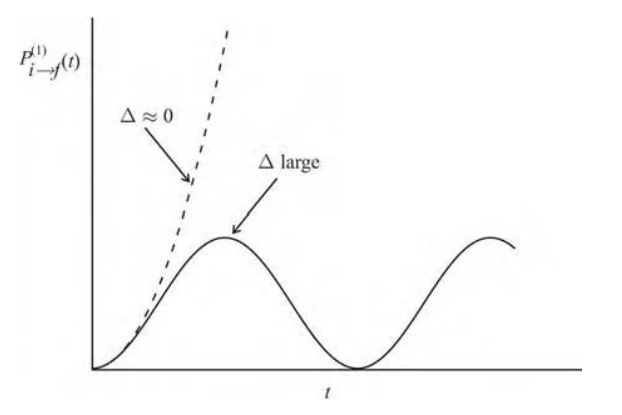
\includegraphics[scale=0.3]{p}
	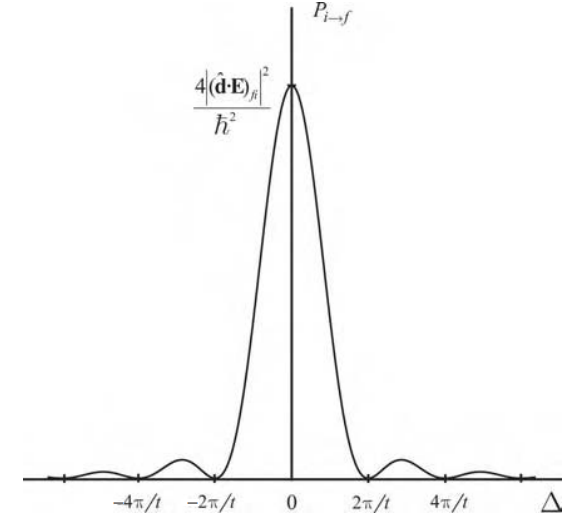
\includegraphics[scale=0.3]{t}
\end{figure}
For the perturbation approximation to be valid we require that $C^{(1)}_f(t) \ll 1$, which implies $P_{i \to f}^{(1)}(t) \ll 1$. For $\Delta \neq 0$, this places constraints on both $\abs{\lp \hat{\mathbf{d}}\cdot\mathbf{E}_0 \rp_{fi}}$ and $\Delta$. On resonance, \eqref{resonance} is only valid for a very short time. For the case of the transition probability as a function of $\Delta$, the width of the peak is proportional to $t^{-1}$ while the height is proportional to $t^2$. It turns out that the area is proportional to $t$:
\begin{align}
\int^{\infty}_{-\infty} \f{\sin^2 \Delta t/2}{\Delta^2} \,d\Delta = \f{\pi t}{2}
\end{align}
In the limit where $\Delta \approx 0$ and $t \gg 2\pi/\omega_{fi}$, the function in the integrand may be approximated by the Dirac delta function
\begin{align}
\lim_{t\to\infty}\f{\sin^2 \Delta t/2}{\Delta^2} = \f{\pi}{2}t\delta(\Delta).
\end{align}
In this case the transition probability is
\begin{align}
P^{(1)}_{i\to f}(t) = \f{\pi}{2}\abs{C^{(1)}_f(t)}^2 = \f{\abs{\lp \hat{\mathbf{d}}\cdot\mathbf{E}_0 \rp_{fi}}^2}{\hbar^2} t \delta(\Delta).
\end{align}
Now we define the time-independent transition probability \textbf{rate} as
\begin{align}
W_{i\to f} = \f{P^{(1)}_{i\to f}}{t} = \f{\pi}{2} \f{\abs{\lp \hat{\mathbf{d}}\cdot\mathbf{E}_0 \rp_{fi}}^2}{\hbar^2} \delta(\omega - \omega_{fi}).
\end{align}
In practice, the driving field will not be monochromatic so that a range of
frequencies will have to be summed or integrated over to obtain the total transition rate.  If $[f]$ represents a set of accessible final states, then the transition rate for a monochromatic field is
\begin{align}
\boxed{W_{i\to [f]} = \f{\pi}{2}\sum_{[f]}\f{\abs{\lp \hat{\mathbf{d}}\cdot\mathbf{E}_0 \rp_{fi}}^2}{\hbar^2} \delta(\omega - \omega_{fi})}
\end{align}
This expression is often famously called Fermi's Golden Rule. Now suppose there is a broad range of frequencies. This means the amplitude of the light is now frequency dependent $\mathbf{E}_0 \to \mathbf{E}_0(\omega)$. Thus the transition probability rate induced by all the frequency components must be
\begin{align}
\f{P^{(1)}_{i\to f}}{t} &=  \int \, d\omega \f{\abs{\lp \hat{\mathbf{d}}\cdot\mathbf{E}_0 \rp_{fi}}^2}{\hbar^2} \f{\sin^2(\Delta t/2)}{\Delta^2}\\
&= \f{1}{\hbar}\int \,d\omega \f{\sin^2(\Delta t/2)}{\Delta^2} \underbrace{\abs{\bra{f}\hat{\mathbf{d}\cdot\mathbf{E}_0(\omega)}\ket{i}}^2}_{F(\omega)}.
\end{align}
Now if $F(\omega)$ varies slowly with $\omega$ compared to $\f{\sin^2(\Delta t/2)}{\Delta^2}$ then we can take $F(\omega)$ to be its resonant value $F(\omega_{fi})$. With this we can take it out of the integral and get
\begin{align}
W_{i\to f} = \f{P^{(1)}_{i\to f}}{t} = \f{\pi}{2\hbar^2}F(\omega_{fi}).
\end{align}
The spread of the frequencies results in the dephasing of the oscillations as shown in the plot of transition probability versus time. This is due to the fact that the light in \textit{incoherent} (lacking the phase relations between the various frequency components). If the atom is driven by coherent light (like a laser), dephasing don't occur and the perturbative time-independent transition rates above generally do not adequately describe the dynamics. We will resolve this issue later. 






 
\subsection{Interaction of an atom with a quantized field \& Spontaneous emission}

In the previous subsection, we did not make any assumption about the relative position of the states $i$ and $f$, i.e., whether $E_i$ is greater or less than $E_f$. We simply said that so long as $\mathbf{E}_0 \neq 0$ and $E_i \neq E_f$, there is some non-zero transition probability. In this section, we will now show that for the case $E_i > E_f$, when the field is quantized, transitions will occur even when no photons are present. This is called \textit{spontaneous emission}. This is one of many differences that appear when we treat the field quantum mechanically versus classically. \\

Let us revisit the single-mode free space field given by \eqref{dipoleE} after dipole approximation (where we assumed the field is uniform over the atom):
\begin{align}
\hat{\mathbf{E}}(\mathbf{r},t)  \approx \hat{\mathbf{E}}(t) = i \lp \f{\hbar\omega_k}{2\epsilon_0 V} \rp^{\f{1}{2}}\mathbf{e} \lb \hat{a}e^{-i\omega t} - \hat{a}^\dagger e^{i\omega t} \rb.
\end{align}
But also recall that this free-space field is written in the Heisenberg picture (there is a time-dependence when the field operator is expressed in the Heisenberg basis). In the Schr\"{o}dinger picture, though, the field operator becomes
\begin{align}
\hat{\mathbf{E}} = i \lp \f{\hbar\omega_k}{2\epsilon_0 V} \rp^{\f{1}{2}}\mathbf{e} \lb \hat{a} - \hat{a}^\dagger \rb.
\end{align}

Now, the free-space Hamiltonian $\hat{\ham}_0$ must be
\begin{align}
\hat{\ham}_0 = \hat{\ham}_\text{atom} + \hat{\ham}_\text{field}
\end{align}
where $\hat{\ham}_\text{atom}$ is just the free-atom Hamiltonian as before and $\hat{\ham}_\text{field}$ is the free-space field Hamiltonian, which we have seen before as well:
\begin{align}
\hat{\ham}_\text{field} = \hbar\omega\lp \hat{a}^\dagger\hat{a} + \f{1}{2} \rp.
\end{align}
Now, because the zero-point energy term does not contribute to the dynamics, we will simply drop it. With this, the interaction Hamiltonian is given by
\begin{align}
\hat{\ham}^{(I)} = -\hat{\mathbf{d}} \cdot\hat{\mathbf{E}} = - i \lp \f{\hbar\omega_k}{2\epsilon_0 V} \rp^{\f{1}{2}}\lp \hat{\mathbf{d}}\cdot\mathbf{e} \rp \lp \hat{a} - \hat{a}^\dagger\rp.
\end{align}
Let us define
\begin{align}
\bm{\mathcal{E}}_0 = i \lp \f{\hbar\omega_k}{2\epsilon_0 V} \rp^{\f{1}{2}}\mathbf{e}.
\end{align}
From this,
\begin{align}
\hat{\ham}^{(I)} = - \hat{\mathbf{d}}\cdot\bm{\mathcal{E}}_0\lp \hat{a} - \hat{a}^\dagger\rp.
\end{align}

Now, because both the atomic and field systems are quantized, the states of the combined system is the product of the states of both the atom and field. Suppose initially we're given the initial state of the atom $\ket{a}$ and $n$ photons $\ket{n}$, then the initial state of the system is
\begin{align}
\ket{i} = \ket{a}\ket{n}. 
\end{align} 
The perturbation interaction of the quantized field causes a transition to the new state 
\begin{align}
\ket{f_1} = \ket{b}\ket{n-1}
\end{align}
where $n-1$ means that one photon has been absorbed by the atom to transition from $\ket{a}$ to $\ket{b}$, or to the state
\begin{align}
\ket{f_2} = \ket{b}\ket{n+1}
\end{align}
where $n+1$ means that one photon has been emitted by the atom to transition from $\ket{a}$ to $\ket{b}$. The energy of these states are
\begin{align}
&\text{for } \ket{i} = \ket{a}\ket{n}, \quad\quad\quad\, E_i = E_a + n\hbar\omega \\
&\text{for } \ket{f_1} = \ket{b}\ket{n-1}, \quad E_i = E_b + (n-1)\hbar\omega \\
&\text{for } \ket{f_2} = \ket{b}\ket{n+1}, \quad E_i = E_b + (n+1)\hbar\omega
\end{align}
where $E_a$ and $E_b$ are the energies of the atomic states $\ket{a}$ and $\ket{b}$. \\

We observe that the interaction Hamiltonian (or the Hamiltonian associated with the perturbation) is time-independent. The matrix elements of this interaction can be calculated by finding
\begin{align}
\text{Absorption: } &\bra{f_1}\hat{\ham}^{(I)}\ket{i}\\
\text{Emission: } &\bra{f_2}\hat{\ham}^{(I)}\ket{i}.
\end{align}
For absorption, we need a term in the interaction Hamiltonian that contains only the annihilation operator:
\begin{align}
\textbf{Absorption: } \bra{f_1}\hat{\ham}^{(I)}\ket{i}
&= \bra{b, n-1}-\hat{\mathbf{d}}\cdot\bm{\mathcal{E}}_0(\hat{a})\ket{a,n}\\
&= \bra{b,n-1}-\hat{\mathbf{d}}\cdot\bm{\mathcal{E}}_0 \sqrt{n}\ket{a,n-1}\\
&= \bra{b}-\hat{\mathbf{d}}\cdot\bm{\mathcal{E}}_0\ket{a}\sqrt{n}\braket{n-1}\\
&= \boxed{-\lp \hat{\mathbf{d}}\cdot\bm{\mathcal{E}}_0 \rp_{ba}\sqrt{n}}
\end{align}
Similarly, for emission
\begin{align}
\textbf{Emission: } \bra{f_2}\hat{\ham}^{(I)}\ket{i}
&= \bra{b, n+1}-\hat{\mathbf{d}}\cdot\bm{\mathcal{E}}_0(-\hat{a}^\dagger)\ket{a,n}\\
&= \bra{b,n+1}\hat{\mathbf{d}}\cdot\bm{\mathcal{E}}_0 \sqrt{n+1}\ket{a,n+1}\\
&= \bra{b}\hat{\mathbf{d}}\cdot\bm{\mathcal{E}}_0\ket{a}\sqrt{n+1}\braket{n+1}\\
&= \boxed{\lp \hat{\mathbf{d}}\cdot\bm{\mathcal{E}}_0 \rp_{ba}\sqrt{n+1}}
\end{align}
where
\begin{align}
\lp \hat{\mathbf{d}}\cdot\bm{\mathcal{E}}_0 \rp_{ba} = \bra{b}\hat{\mathbf{d}}\cdot\bm{\mathcal{E}}_0\ket{a} = \bra{b}\hat{\mathbf{d}}\ket{a}\cdot\bm{\mathcal{E}}_0 \equiv \mathbf{d}_{ba}\cdot\bm{\mathcal{E}}_0
\end{align}
is the dipole matrix element between states $\ket{b}$ and $\ket{a}$. \\

It is worthy to compare this result to the semiclassical picture we saw in the last subsection. For the absorption case, there is nothing new: if no field then no absorption: 
\begin{align}
n=0 \implies \bra{f_1}\hat{\ham}^{(I)}\ket{i} = 0
\end{align}
since $\sqrt{n} = 0$. However, the emission case has no semiclassical counterpart: transitions may occur even when no photons are present:
\begin{align}
n=0 \centernot\implies \bra{f_2}\hat{\ham}^{(I)}\ket{i} = 0
\end{align}
since $\sqrt{n+1}\neq 0$. This is called \textbf{spontaneous emission}, which cannot be obtained from the semiclassical approach. If $n > 0$, the emission of an additional photon is called \textbf{stimulated emission}, which is essential for the operation of the ``light amplification by stimulated emission of radiation'' or LASER. \\

We might also be interested in the ratio of the absorption/emission rates:
\begin{align}\label{rates}
\boxed{\f{\abs{\bra{f_2}\hat{\ham}^{(I)}\ket{i}}^2}{\abs{\bra{f_1}\hat{\ham}^{(I)}\ket{i}}^2}= \f{n+1}{n}}
\end{align}

It turns out that we can still use the perturbation method developed in the previous section to calculate the transition amplitudes, provided that me make appropriate modifications to account for the fact that the field is now quantized. The first difference is in the Hamiltonians:
\begin{align}
\hat{\ham}_0 = \hat{\ham}_\text{atom}  &\to \hat{\ham}_0 =  \hat{\ham}_\text{atom} + \hat{\ham}_\text{field}\\
\hat{\ham}^{(I)}(t) = -\hat{\mathbf{d}}\cdot\mathbf{E}(t) &\to \hat{\ham}^{(I)}(t) = - \hat{\mathbf{d}}\cdot\bm{\mathcal{E}}_0\lp \hat{a} - \hat{a}^\dagger\rp
\end{align}
where of course
\begin{align}
\hat{\ham}_\text{field} = \hbar\omega\lp \hat{a}^\dagger\hat{a} + \f{1}{2} \rp
\end{align}
where we again leave out the zero-point energy term. \\

Now, let us assume that the atom has only two levels $\ket{a}$ and $\ket{b}$. The state vector of the system can be written as
\begin{align}
\ket{\psi(t)} = &C_i(t)\ket{a}\ket{n}e^{-i\omega_a t}e^{-i n \omega t } \nonumber\\
&+ C_{f_1}(t)\ket{b}\ket{n-1}e^{-i\omega_b t}e^{-i (n-1) \omega t } \nonumber\\
&+ C_{f_2}(t)\ket{b}\ket{n+1}e^{-i\omega_b t}e^{-i (n+1) \omega t } 
\end{align}
where the first term is the initial state of the system, the second term is corresponds to absorption, and the third term corresponds to emission. We assume that $\ket{\psi(t)} = \ket{a}\ket{n}$, $C_i(0) = 1$, and $C_{f_1}(0) = C_{f_2}(0) = 0$. Following the perturbative method used before, we can get the first-order correction
for the amplitudes $C_{f_1}$ and $C_{f_2}$ associated with the atom being in state $\ket{b}$:
\begin{align}
\text{Absorption: }&C_{f_1}^{(1)}(t) = -\f{i}{\hbar}\int_0^t \,dt' \bra{f_1}\hat{\ham}^{(I)}\ket{i}e^{i(\omega_{f_1} - \omega_i)t'}\\
\text{Emission: }&C_{f_2}^{(1)}(t) = -\f{i}{\hbar}\int_0^t \,dt' \bra{f_2}\hat{\ham}^{(I)}\ket{i}e^{i(\omega_{f_2} - \omega_i)t'}.
\end{align}
And so the amplitude of the atom being in state $\ket{b}$ (to first-order of course) regardless of how it got there is the \textit{sum} of these amplitudes:
\begin{align}\label{quantum_amp}
C_f^{(1)}(t) &= C_{f_1}^{(1)}(t) + C_{f_2}^{(1)}(t)\\
&= \f{i}{\hbar}\lp \hat{\mathbf{d}}\cdot\bm{\mathcal{E}}_0 \rp_{ba}\int^t_0 \,dt'  \sqrt{n}  e^{i(\omega_{f_1} - \omega_i)t'} 
- \sqrt{n+1}  e^{i(\omega_{f_2} - \omega_i)t'}\\
&= \boxed{\f{i}{\hbar}\lp \hat{\mathbf{d}}\cdot\bm{\mathcal{E}}_0 \rp_{ba}
\lb \underbrace{\sqrt{n+1}\cdot\f{e^{i(\omega + \omega_{ba})t} - 1}{ \omega + \omega_{ba} }}_\text{Emission}  - \underbrace{\sqrt{n}\cdot\f{e^{i(\omega - \omega_{ba})t} - 1}{\omega - \omega_{ba}}}_{\text{Absorption}}\rb}
\end{align}
If $n\ll 1$ then $\sqrt{n+1} \approx \sqrt{n}$, in which case this result and \eqref{amplitude} are essentially the same and we get a correspondence between classical and quantum field amplitudes:
\begin{align}
\lp \mathbf{E}_0 \rp_\text{classical} \leftrightarrow \lp 2i\mathcal{E}_0\sqrt{n} \rp_\text{quantum}.
\end{align}

If $E_b > E_a$ ($\ket{b}$ is the excited state) and $\omega \approx \omega_{ba}$ then by RWA the first term in \eqref{quantum_amp} can be dropped as the second term dominates. There is nothing abnormal about this. However, if $E_a > E_b$ ($\ket{a}$ is the excited state) and $\omega \approx -\omega_{ba}$, then the second term of \eqref{quantum_amp} can be dropped (again under RWA). This leaves us with
\begin{align}
C_f^{(1)}(t) \approx \f{i}{\hbar}\lp \hat{\mathbf{d}}\cdot\bm{\mathcal{E}}_0 \rp_{ba}
\lb \underbrace{\sqrt{n+1}\cdot\f{e^{i(\omega + \omega_{ba})t} - 1}{ \omega + \omega_{ba} }}_\text{Emission}\rb.
\end{align}
We notice that even when $n=0$, this does not vanish. In this case, the transition between $\ket{a}$ and $\ket{b}$ occurs through spontaneous emission. 




\subsubsection{Field-theoretic derivation of the Planck's distribution}

Suppose we have a collection of atoms interacting resonantly with a quantized field of frequency
\begin{align}
\omega = \f{E_a - E_b}{\hbar}
\end{align}
where $\ket{a}$ and $\ket{b}$ are atomic eigenstates with $E_a > E_b$. Let $N_a, N_b$ be the populations of atoms in $\ket{a}$ and $\ket{b}$ respectively. Let $W_\text{emis}$ and $W_\text{abs}$ be the transition rate due to photon emission and absorption respectively. We have the following set of differential equations:
\begin{align}
&\f{dN_a}{dt} = -N_a W_\text{emis} + N_b W_\text{abs}\\
&\f{dN_b}{dt} = -N_b W_\text{abs} + N_a W_\text{emis}.
\end{align}
At thermal equilibrium:
\begin{align}
\f{dN_a}{dt} = 0 = \f{dN_b}{dt} \implies N_a W_\text{emis} = N_b W_\text{abs}.
\end{align}
From the relative rates in \eqref{rates}, we have
\begin{align}\label{1}
\f{N_b}{N_a} = \f{W_\text{emis}}{W_\text{abs}} = \f{n+1}{n}.
\end{align}
Now, according to Boltzmann statistics:
\begin{align}\label{2}
\f{N_b}{N_a} = e^{(E_a - E_b)/kT} = e^{\hbar\omega /kT}. 
\end{align}
From \eqref{1} and \eqref{2} we have
\begin{align}
\boxed{n = \f{1}{e^{\hbar\omega/kT} - 1}}
\end{align}

There's a slightly different derivation by Einstein (which was done even before quantum electrodynamics was invented), which takes into account as well the distinction between spontaneous and stimulated emission. We won't go into the details of this. 



\subsection{The Rabi model}

In the previous subsections we have used the perturbation theory approach to calculate transition probabilities. This approach assumes that the population in the initial state is essentially unchanged and the population in the final states are very small. This approach fails in cases of large population transfer, for example when there is a strong, near resonance (with one state and no other) laser field. In this case, the perturbation approach must be abandoned, only two dominant states remain, and the problem can solved ``exactly.'' This is the \textbf{Rabi model}. We note that the Rabi model is a \textit{semiclassical model}. The full quantum mechanical model is covered in the next subsection. \\

Suppose our two levels are the ground $\ket{g}$ and excited state $\ket{e}$. The transition frequency is given by
\begin{align}
\omega_0 = \f{E_e - E_g}{\hbar} \approx \omega
\end{align}
where $\omega$ is the frequency of the driving field. Once again, the interaction Hamiltonian is given by
\begin{align}
\hat{\ham}^{(I)} = -\hat{\mathbf{d}}\cdot\mathbf{E}_0 \cos\omega t \equiv \hat{V}_0 \cos\omega t
\end{align}
where again the dipole approximation is already made. The state vector is a linear combination of the eigenstates:
\begin{align}
\ket{\psi(t)} = C_g(t)e^{-iE_gt/\hbar}\ket{g} + C_e(t)e^{-iE_et/\hbar}\ket{e}.
\end{align}
The Schr\"{o}dinger equation
\begin{align}
i\hbar \f{\p \ket{\psi(t)}}{\p t} &= \lp \hat{\ham}_0 + \hat{\ham}^{(I)} \rp \ket{\psi(t)}\\
&=\lp \hat{\ham}_0 + \hat{V}_0 \cos\omega t \rp \ket{\psi(t)}
\end{align}
gives a system of differential equations:
\begin{align}
\begin{bmatrix}
\dot{C}_g \\ \dot{C}_e
\end{bmatrix}
=
\begin{bmatrix}
0 &-\f{i}{\hbar}\bra{g}\hat{V}_0 \ket{e}e^{-i\omega_0 t} \\ 
-\f{i}{\hbar}\bra{g}\hat{V}_0 \ket{e}e^{i\omega_0 t} & 0
\end{bmatrix}
\begin{bmatrix}
C_g \\ C_e
\end{bmatrix}
\end{align}
where the first equation is obtained by multiplying the SE from the left by $e^{i\omega_g t}\bra{g}$ and the fact that $\bra{i}\hat{V}_0\ket{j} = 0$ when $i = j$. Next, we assume that $\bra{g}\hat{V}_0 \ket{e}$ is real and $C_g(0) = 1, C_e(0) = 0$. Let us call
\begin{align}
\mathcal{V} = \bra{g}\hat{V}_0 \ket{e}
\end{align}
and approximate $\cos\omega t$ in exponentials and keep only the terms that oscillate at frequency $\omega - \omega_0$ to get
\begin{align}
&\dot{C}_g = -\f{i}{2\hbar}\mathcal{V}e^{i(\omega - \omega_0 )t}C_e\\
&\dot{C}_e = -\f{i}{2\hbar}\mathcal{V}e^{-i(\omega - \omega_0 )t}C_g.
\end{align}
Taking the derivative of the second equation, plugging it into the first while applying RWA (eliminating terms with $\omega + \omega_0$) we get
\begin{align}
\ddot{C}_e + i(\omega - \omega_0 )\dot{C}_e + \f{1}{4}\f{\mathcal{V}^2}{\hbar^2}C_e = 0.
\end{align}
This differential equation is quite a classic. The general solution is
\begin{align}
C_e(t) = A_+ e^{i\lambda_+ t} + A_- e^{i\lambda_- t} 
\end{align}
where with $\Delta = \omega - \omega_0$,
\begin{align}
\lambda_{\pm} = \f{1}{2}\lb \Delta \pm \sqrt{ \Delta^2 + \f{\mathcal{V}^2}{\hbar^2}} \rb.
\end{align}
From the initial conditions, we also have that
\begin{align}
A_{\pm} = \mp \f{1}{2\hbar}\f{\mathcal{V}}{\sqrt{\Delta^2 + \f{\mathcal{V}^2}{\hbar^2}}}.
\end{align}
With this, the solution to the problem is
\begin{align}
&C_e(t) = i\f{\mathcal{V}}{\Omega_R \hbar}e^{i\Delta t/2}\sin\f{\Omega_R t}{2}\\
&C_g(t) = e^{i\Delta t/2} \lc \cos\f{\Omega_R t}{2} - i\f{\Delta}{\Omega_R}\sin\f{\Omega_R t}{2} \rc
\end{align}
where
\begin{align}
\Omega_R = \sqrt{\Delta^2 + \f{\mathcal{V}^2}{\hbar^2}}
\end{align}
is called the \textbf{Rabi frequency}, or \textbf{Rabi rate}. \\

The probability that the atom is in the excited state $\ket{e}$ is then
\begin{align}
\boxed{P_e(t) = \abs{C_e(t)}^2 = \f{\mathcal{V}^2}{\Omega_R^2\hbar^2}\sin^2\f{\Omega_R t}{2}}
\end{align}
On resonance, this probability is a perfect sine-squared:
\begin{align}
\boxed{P_e(t) = \sin^2\f{\mathcal{V}t}{2\hbar}}
\end{align}
where at $t= \pi \hbar / \mathcal{V}$ all the atomic population is transferred to the excited state. The following plot illustrates the population transfer and ``oscillation''
\begin{figure}[!htb]
	\centering
	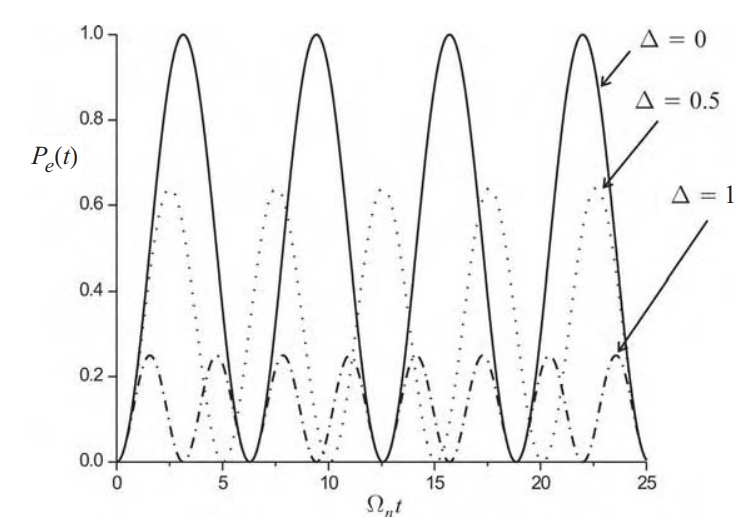
\includegraphics[scale=0.3]{rabi}
\end{figure}

The \textbf{atomic inversion} $W(t)$ is defined as the difference in population between the excited and ground states:
\begin{align}
W(t) = P_e(t) - P_g(t).
\end{align}
For the case of resonance ($\Delta = 0$) and that initially the atom is in the ground state, 
\begin{align}
W(t) = \sin^2 \f{\mathcal{V}t}{2\hbar} - \cos^2 \f{\mathcal{V}t}{2\hbar} = -\cos\f{\mathcal{V}t}{\hbar} = -\cos\Omega_R(\Delta = 0)t.
\end{align}
For $t = \pi\hbar/\mathcal{V}$, $W(\pi\hbar/\mathcal{V}) = 1$. This kind of population transfer is called the $\pi-$pulse. For $t = \pi\hbar/2\mathcal{V}$, $W(\pi\hbar/2\mathcal{V}) = 0$, which means the population is shared coherently between the ground and excited states, i.e., the system is in a perfect superposition:
\begin{align}
\ket{\psi(t)} = \f{1}{\sqrt{2}}\lp\ket{g} + i\ket{e} \rp.
\end{align}










\subsection{Fully quantum-mechanical model; the Jaynes–Cummings model}

We move on to the quantum electrodynamics version of the Rabi model. In our previous discussion of the interaction between atoms and the quantized field, we assumed the field is single-mode. We again assume this, such that the single-mode cavity field can be written as
\begin{align}
\mathbf{\hat{E}} = \mathbf{e}\lp \f{\hbar\omega}{\epsilon_0 V} \rp^{1/2}\lp \hat{a} + \hat{a}^\dagger\rp\sin(kz)
\end{align}
where $\mathbf{e}$ is some arbitrary polarization vector. We also assume that the atom has two levels $\ket{g}$ and $\ket{e}$. The interaction Hamiltonian is given by
\begin{align}
\hat{\ham}^{(I)} = -\mathbf{\hat{d}} \cdot \mathbf{\hat{E}} = \hat{d} g (\hat{a} + \hat{a}^\dagger)
\end{align}
where
\begin{align}
\hat{d} &= \mathbf{d} \cdot \mathbf{e}\\
g &=  \lp \f{\hbar\omega}{\epsilon_0 V} \rp^{1/2}\sin(kz).
\end{align}

For simplicity, let us introduce the atomic transition operators 
\begin{align}
\text{Excitation: } &\hat{\sigma}_+ = \ket{e}\bra{g}\\
\text{De-excitation: } &\hat{\sigma}_- = \ket{g}\bra{e} = \hat{\sigma}_+^\dagger.
\end{align}
The inversion operator is given by
\begin{align}
\hat{\sigma}_3 = \ket{e}\bra{e} - \ket{g}\bra{g}.
\end{align}
We can verify that these operators obey the Pauli spin algebra:
\begin{align}
[\hat{\sigma}_+, \hat{\sigma}_-] &= \hat{\sigma}_3\\
[\hat{\sigma}_3, \hat{\sigma}_\pm] &= 2\hat{\sigma}_\pm.
\end{align}

We know that the diagonal matrix elements of $\hat{d}$ is zero because $\bra{e}\hat{d}\ket{e} = \bra{g}\hat{d}\ket{g} = 0$. This means with $d = \bra{e}\hat{d}\ket{g}$, we can write in the basis
\begin{align}
\hat{d} &= d\ket{g}\bra{e} + d^*\ket{e}\bra{g}\\
&= d\hat{\sigma}_- + d^*\hat{\sigma}_+\\
&= d\lp \hat{\sigma}_- + \hat{\sigma}_+ \rp.
\end{align}
This gives the interaction Hamiltonian:
\begin{align}
\hat{\ham}^{(I)} = \hbar \lp \f{dg}{\hbar} \rp \lp \hat{\sigma}_- + \hat{\sigma}_+ \rp \lp \hat{a} + \hat{a}^\dagger \rp. 
\end{align}
Define the energy to be zero halfway between the states, then we have $E_e = -E_g$, and the free atomic Hamiltonian can be written as
\begin{align}
\hat{\ham}_0 = \f{\hbar}{2}\begin{bmatrix}
E_e & \\ & E_g
\end{bmatrix} 
\end{align}
or in the basis
\begin{align}
\hat{\ham}_0 = \f{1}{2}\hbar\omega_0 \lp \ket{e}\bra{e} - \ket{g}\bra{g} \rp = \f{1}{2}\hbar\omega_0 \hat{\sigma}_3 
\end{align}
where 
\begin{align}
E_e = -E_g = \f{1}{2}\hbar\omega_0
\end{align}
and of course $\omega_0$ is the transition frequency. The free-field Hamiltonian after dropping the zero-point energy term, again, is
\begin{align}
\hat{\ham}_F = \hbar\omega\hat{a}^\dagger\hat{a}.
\end{align}
So the total Hamiltonian is
\begin{align}
\hat{\ham} &= \hat{\ham}_0 + \hat{\ham}_F + \hat{\ham}^{(I)}\\
&= \f{1}{2}\hbar\omega_0 \hat{\sigma}_3  + \hbar\omega\hat{a}^\dagger\hat{a} + \hbar \lp \f{dg}{\hbar} \rp \lp \hat{\sigma}_- + \hat{\sigma}_+ \rp \lp \hat{a} + \hat{a}^\dagger \rp.
\end{align}
Let us call
\begin{align}
\lambda = \f{dg}{h}.
\end{align}
It follows that
\begin{align}
\hat{\ham} = \f{1}{2}\hbar\omega_0 \hat{\sigma}_3  + \hbar\omega\hat{a}^\dagger\hat{a} + \hbar \lambda\lp  \hat{\sigma}_- + \hat{\sigma}_+ \rp \lp \hat{a} + \hat{a}^\dagger \rp.
\end{align}
Let us simplify this Hamiltonian with some approximations. We know that in the field-free case, the creation and annihilation operators evolve in time as
\begin{align}
\hat{a}(t) = \hat{a}(0)e^{-i\omega t} \hspace{0.5cm} \hat{a}^\dagger(t) = \hat{a}^\dagger(0)e^{i\omega t},
\end{align}
while in the free atomic case the excitation operators (which we can show) to evolve in time as
\begin{align}
\hat{\sigma}_{\pm}(t) = \hat{\sigma}_\pm(0)e^{\pm i \omega_0 t}.
\end{align}
This gives us some idea of the time dependency of the product of some of these operators:
\begin{align}
&\hat{\sigma}_+ \hat{a} \sim e^{i(\omega_0 - \omega)t}\\
&\hat{\sigma}_- \hat{a}^\dagger \sim e^{-i(\omega_0 - \omega)t}\\
&\hat{\sigma}_+ \hat{a}^\dagger \sim e^{i(\omega_0 + \omega)t}\\
&\hat{\sigma}_- \hat{a} \sim e^{-i(\omega_0 + \omega)t}.
\end{align}
For $\omega_0 \approx \omega$ we can use RWA to ignore the last two terms. The term $\hat{\sigma}_+ \hat{a}^\dagger$ corresponds to the emission of a photon (the creation operator) as the atom goes from the ground to the excited state, while the term $\hat{\sigma}_- \hat{a}$ corresponds to the absorption of a photon (the annihilation operator) as the atom goes from the excited to ground state. It makes good sense to ignore these terms, so that we're left with the approximate Hamiltonian:
\begin{align}
\boxed{\hat{\ham} = \f{1}{2}\hbar\omega_0 \hat{\sigma}_3  + \hbar\omega\hat{a}^\dagger\hat{a} + \hbar \lambda\lp  \hat{\sigma}_+ \hat{a}  + \hat{\sigma}_-\hat{a}^\dagger \rp}
\end{align}
This is called the \textbf{Jaynes-Cummings model}. To solve the dynamics of the system, we first note a few constants. The first constants is the number of electrons, or the total probability of the atom being in either state $\ket{e}$ or $\ket{g}$:
\begin{align}
\hat{P}_E = \ket{e}\bra{e} + \ket{g}\bra{g} = 1.
\end{align}
and of course this quantity is conserved: 
\begin{align}
[\hat{\ham}, \hat{P}_E] \propto \f{d\hat{P}_E}{d t} = 0.
\end{align}
The excitation number is also unchanged: 
\begin{align}
\hat{N}_e = \hat{a}^\dagger\hat{a} + \ket{e}\bra{e} \implies [\hat{\ham}, \hat{N}_e] \propto \f{d\hat{N}_e}{dt} = 0.
\end{align}
This equation essentially says the number of electrons created corresponds to the transitions.\\

With these constants we may break the Hamiltonian into two commuting parts:
\begin{align}
\hat{\ham} = \hat{\ham}_I + \hat{\ham}_{II}
\end{align}
where
\begin{align}
\hat{\ham}_I &= \hbar\omega \hat{N}_e + \hbar\lp \f{\omega_0}{2} - \omega \rp\hat{P}_E\\
\hat{\ham}_{II} &= -\hbar\Delta + \hbar \lambda \lp \hat{\sigma}_+ \hat{a}  + \hat{\sigma}_-\hat{a}^\dagger \rp
\end{align}
All dynamics is contained in $\hat{H}_{II}$, while $\hat{\ham}_I$ contributes to (irrelevant) phase factors. Next, let us examine a few notable cases. 

\subsubsection{Resonance: $\Delta = 0$}

Let us assume that initially the atom is in the excited state $\ket{e}$ and the field is initially in the state $\ket{n}$. The initial atom-field state is
\begin{align}
\ket{i} = \ket{e}\ket{n}.
\end{align}
The energy of this state is of course
\begin{align}
E_i  = E_e + E_n = \f{1}{2}\hbar\omega + n\hbar\omega
\end{align}
where recall that we have set zero energy to be in the middle of the two states. This initial state $\ket{i}$ to coupled to and only to the final state $\ket{f} = \ket{g}\ket{n+1}$. The state vector is given by
\begin{align}
\ket{\psi(t)} = C_i(t) \ket{i} + C_f(t)\ket{f}
\end{align}
with $C_i(0) = 1$ and $C_f(0) = 0$. In the interaction picture, 
\begin{align}
i\hbar \f{d\ket{\psi(t)}}{dt} = \hat{\ham}_{II}\ket{\psi(t)}.
\end{align}
Plugging $\hat{\ham}_{II}$ in and solve we obtain
\begin{align}
\dot{C}_i &= -i\lambda \sqrt{n+1}C_f\\
\dot{C}_f &= -i\lambda \sqrt{n+1}C_i. 
\end{align}
By eliminating $C_f$ and solving, we get 
\begin{align}
C_i(t) = \cos\lp  \lambda t \sqrt{n+1} \rp
\end{align}
and 
\begin{align}
C_f(t) =-i\sin\lp \lambda t \sqrt{n+1} \rp.
\end{align}
With this, the probability that the system is in the initial state is
\begin{align}
P_i(t) = C_i^*(t)C_i(t) = \cos^2 \lp  \lambda t \sqrt{n+1} \rp.
\end{align}
And the probability that the system is in the other state is of course
\begin{align}
P_f(t) = \sin^2\lp  \lambda t \sqrt{n+1} \rp.
\end{align}
The atom inversion is then
\begin{align}
W(t) = P_i(t) - P_f(t) = \cos\lp 2\lambda t \sqrt{n+1} \rp.
\end{align}
We may define a quantum electrodynamic Rabi frequency
\begin{align}
\boxed{\Omega(n) = 2\lambda\sqrt{n+1}}
\end{align}
This gives
\begin{align}
W(t) = \cos\lp \Omega(n)t \rp.
\end{align}
We notice that there's Rabi oscillation, which we also see in the classical case. However, there is still Rabi oscillation in the case of $n=0$. These is vacuum Rabi oscillation. They are the result of the atom spontaneously emitting a photon then re-absorbing it, re-emitting it, etc.: an example of reversible spontaneous emission.


\subsubsection{Pure state}
In this scenario we assume that the atom is initially in a superposition of $\ket{e}$ and $\ket{g}$. 
\begin{align}
\ket{\psi(t)}_\text{atom} =C_e\ket{e} + C_g\ket{g}.
\end{align}
The field is initially in the state
\begin{align}
\ket{\psi(t)}_\text{field} = \sum_{n=0}^\infty C_n\ket{n}.
\end{align}
Thus the initial state of the system is given by a tensor product
\begin{align}
\ket{\psi(t)} = \ket{\psi(0)}_\text{atom} \otimes \ket{\psi(0)}_\text{field}.
\end{align}
The solution to the Schr\"{o}dinger equation is now
\begin{align}
\ket{\psi(t)} = \sum^\infty_{n=0}\lc \lb C_e C_n \cos (\lambda t \sqrt{n+1}) - iC_gC_{n+1}\sin(\lambda t \sqrt{n+1}) \rb \ket{e} \right. \nonumber \\  \left.
+ \lb -iC_eC_{n-1}\sin(\lambda t \sqrt{n}) + C_gC_n \cos(\lambda t \sqrt{n}) \rb 
 \rc \otimes \ket{n}.
\end{align}
This is an entangled state. Now, if $C_e = 1$ and $C_g = 0$ initially, then
\begin{align}
\ket{\psi(t)} = \ket{\psi_g(t)}\otimes \ket{g} + \ket{\psi_e(t)}\otimes \ket{e},
\end{align}
where
\begin{align}
&\ket{\psi_g(t)} = -i\sum^\infty_{n=0}C_n\sin(\lambda t \sqrt{n+1})\ket{n+1}\\
&\ket{\psi_e(t)} = \sum^\infty_{n=0}C_n\cos(\lambda t \sqrt{n+1})\ket{n}.
\end{align}
The atomic inversion is then
\begin{align}
W(t) &= \bra{\psi(t)}\hat{\sigma}_3\ket{\psi(t)}\\
&= \braket{\psi_e(t)} - \braket{\psi_g(t)}\\
&= \sum^\infty_{n=0}\abs{C_n}^2 \cos(2\lambda t\sqrt{n+1}).
\end{align}


\subsection{The Density Operator approach (or the master equation's approach) }
So far, we have considered only cases where the field and the atom are initially in pure states. The density operator approach allows us to solve for a more general case. Let us work in the interaction picture again where the interaction Hamiltonian is given by
\begin{align}
\hat{\ham}_I = \hbar\lambda \lp \hat{a}\hat{\sigma}_+ + \hat{a}^\dagger\hat{\sigma}_- \rp
\end{align}
Let us consider the density operator of the atom-field system at time $t$. As we know the density operator is defined to be
\begin{align}
\hat{\rho} = \ket{\psi}\bra{\psi}.
\end{align}
Applying the Schr\"{o}dinger equation to $\ket{\psi}$, we have
\begin{align}
i\hbar \f{d\ket{\psi}}{dt} = \hat{\ham}_I \ket{\psi}.
\end{align}
Now let us see what we get when we look at the time evolution of the density operator
\begin{align}
\f{d \hat{\rho}}{dt} &= \f{d\ket{\psi}}{dt} \bra{\psi} + \ket{\psi}\f{d\bra{\psi}}{dt}\\
&= \lb \f{-i}{\hbar}\hat{\ham}_I\ket{\psi} \rb\bra{\psi} + \ket{\psi}\lb \f{i}{\hbar}\bra{\psi} \hat{\ham}_I \rb\\
&= \f{-i}{\hbar}\lb \hat{\ham}_I\ket{\psi}\bra{\psi} - \ket{\psi}\bra{\psi}\hat{\ham}_I \rb\\
&= \f{-i}{\hbar}\lb \hat{\ham}_I, \hat{\rho} \rb.
\end{align}
The solution to this (which we can quite easily verify) is 
\begin{align}\label{rho}
\hat{\rho}(t) = e^{-i\hat{\ham}_I t/\hbar}\hat{\rho}(0)e^{i\hat{\ham}_I t/\hbar} = \hat{U}_I(t)\hat{\rho}(0)\hat{U}_I^\dagger(t).
\end{align} 
Recall that the Hamiltonian can be expressed further in terms of the excitation/de-excitation, and inversion operators, whose matrix representations are
\begin{align}
\sigma_+ = \begin{bmatrix}
0 & 1\\0 & 0
\end{bmatrix}, \hspace{0.5cm}
\sigma_- = \begin{bmatrix}
0 & 0 \\ 1 & 0
\end{bmatrix}, \hspace{0.5cm}
\sigma_3 = \begin{bmatrix}
1 & 0 \\ 0 & -1
\end{bmatrix}
\end{align}
where we have used the convention
\begin{align}
\sigma_j = \begin{bmatrix}
\bra{e}\hat{\sigma}_j\ket{e} & \bra{e}\hat{\sigma}_j\ket{g}\\
\bra{g}\hat{\sigma}_j\ket{e} &
\bra{g}\hat{\sigma}_j\ket{g} 
\end{bmatrix}, \hspace{0.5cm} j = \pm, 3.
\end{align}
Let us re-write $\hat{U}_I(t)$ in terms of these operators:
\begin{align}
\hat{U}_I(t) = e^{-i\hat{H}_I t/\hbar} = e^{-i\lambda t (\hat{a}\hat{\sigma}_+ + \hat{a}^\dagger\hat{\sigma_-})}.
\end{align}
With this, we can write the evolution operator $\hat{U}_I$ in terms of cosines and sines as
\begin{align}
\hat{U}_I(t) = \begin{bmatrix}
\hat{C}(t) & \hat{S}'(t) \\ \hat{S}(t) & \hat{C}'(t)
\end{bmatrix}
\end{align}
where
\begin{align}
&\hat{C}(t) = \cos(\lambda t \sqrt{\hat{a}\hat{a}^\dagger})\\
&\hat{S}(t) = -i\hat{a}^\dagger\f{\sin(\lambda t \sqrt{\hat{a}\hat{a}^\dagger})}{\sqrt{\hat{a}\hat{a}^\dagger}}\\
&\hat{C}'(t) = \cos(\lambda t \sqrt{\hat{a}^\dagger\hat{a}})\\
&\hat{S}'(t) =  -i\hat{a}\f{\sin(\lambda t \sqrt{\hat{a}^\dagger\hat{a}})}{\sqrt{\hat{a}^\dagger\hat{a}}}.
\end{align}
It is then easy to show that
\begin{align}
\hat{U}^\dagger_I(t) = \hat{U}_I(-t) = \begin{bmatrix}
\hat{C}(t) & -\hat{S}'(t) \\ -\hat{S}(t) & \hat{C}'(t)
\end{bmatrix}.
\end{align}
Now, suppose at $t=0$ the density operator for the atom-field system can be written as a tensor product of the field and atom parts (not entangled):
\begin{align}
\hat{\rho}(0) = \hat{\rho}^F(0)\otimes \hat{\rho}^A(0).
\end{align}
Next, suppose that our atom is initially in $\ket{e}$, such that by convention the atom's density matrix is
\begin{align}
\rho^A(0) = \begin{bmatrix}
1 & 0 \\ 0 & 0
\end{bmatrix}.
\end{align}
Thus for the system,
\begin{align}
\hat{\rho}(0) = \hat{\rho}^F(0) \otimes \begin{bmatrix}
1 & 0 \\ 0 & 0
\end{bmatrix} = \begin{bmatrix}
\hat{\rho}^F(0) & 0 \\ 0 & 0 
\end{bmatrix}.
\end{align}
Now by \eqref{rho},
\begin{align}
\hat{\rho}(t) = \begin{bmatrix}
\hat{C}(t)\hat{\rho}^F(0)\hat{C}(t) & -\hat{C}(t)\hat{\rho}^F(0)\hat{S}'(t)\\
\hat{S}(t)\hat{\rho}^F(0)\hat{C}(t) & -\hat{S}(t)\hat{\rho}^F(0)\hat{S}'(t)
\end{bmatrix}.
\end{align}

To find the density operator of the field, we trace over the atomic states:
\begin{align}
\hat{\rho}^F(t) = \Tr_A \hat{\rho}(t) = \hat{C}(t)\hat{\rho}^F(0)\hat{C}(t) -\hat{S}(t)\hat{\rho}^F(0)\hat{S}'(t).
\end{align}
The matrix elements for the field are then
\begin{align}
\hat{\rho}^F_{nm} &\equiv \bra{n}\hat{\rho}^F(t)\ket{m} \\ 
&= \bra{n} \hat{C}(t)\hat{\rho}^F(0)\hat{C}(t) \ket{m} - \bra{n} \hat{S}(t)\hat{\rho}^F(0)\hat{S}'(t) \ket{m}.
\end{align}
On the other hand, tracing over the field states (there are infinitely many) we obtain the density operator of the atom:
\begin{align}
\hat{\rho}^A(t) = \Tr_F \hat{\rho}(t) = \sum^\infty_{n=0} \bra{n}\hat{\rho}(t)\ket{n}.
\end{align}
The matrix elements are then
\begin{align}
\bra{i}\hat{\rho}^A(t)\ket{j} = \sum^\infty_{n=0}\bra{i,n} \hat{\rho}_F(t)\ket{j,n}
\end{align}
where $i,j = e,g$. The diagonal elements $\rho^A_{ee}$ and $\rho^A_{gg}$ are the populations of the excited and ground states and satisfy
\begin{align}
\rho^A_{gg}(t) + \rho^A_{ee}(t) = 1
\end{align}
for any time $t$. The atomic inversion is
\begin{align}
W(t) = \rho^A_{ee}(t) - \rho^A_{gg}(t) = 2\rho^A_{ee}(t) - 1.
\end{align}
We can find that
\begin{align}
\rho^A_{ee}(t) &= \sum^\infty_{n=0}\bra{n}\hat{C}(t)\hat{\rho}^F(0)\hat{C}(t)\ket{n}\\
&= \sum^\infty_{n=0}\bra{n}\hat{\rho}^F(0)\ket{n}\cos^2(\lambda t \sqrt{n+1}).
\end{align}
\subsubsection{Pure state}
If the field is initially in a pure state
\begin{align}
\ket{\psi_F(0)} = \sum^\infty_{n=0}C_n\ket{n},
\end{align}
then
\begin{align}
\hat{\rho}^F(0) = \ket{\psi_F}\bra{\psi_F},
\end{align}
which gives
\begin{align}
\rho^A_{ee}(t) = \sum^\infty_{n=0}\abs{C_n}^2\cos^2(\lambda t \sqrt{n+1}).
\end{align}
This gives the atomic inversion we have found before. 
\subsubsection{Mixed state}
However, if the field is initially in a thermal state (mixed state) where
\begin{align}
\hat{\rho}^F(0) = \hat{\rho}_{Th} = \sum P_n\ket{n}\bra{n}
\end{align}
where $P_n$ is probability. The atomic inversion in this case is
\begin{align}
W(t) = \sum^\infty_{n=0}P_n \cos(2\lambda t\sqrt{n+1}),
\end{align}
which is slightly different. 



















\newpage

\section{Collective Atomic Interactions}



\newpage
























\chapter{QUANTUM \& CLASSICAL FIELD THEORIES}


\newpage



\section{Path Integral Formulation of QM, Shankar}




So far, we have only been looking at quantum mechanics in the Schr\"{o}dinger formulation, which stems from Hamiltonian mechanics. In this section we will consider the Lagrangian formulation (Hamiltonian's counterpart) of quantum mechanics, which was invented by Richard Feynman in the 1940s. The path integral formulation of quantum mechanics is not only beautiful but it also can for a certain class of problems give us the full propagator with ease. This formulation also gives us better insights into the relationship between classical and quantum mechanics. \\


\subsection{The recipe}


In the Schr\"{o}dinger approach, which I hope we have seen enough at this point, we find the propagator $U$ by first evaluating the eigenvalues of the Hamiltonian, and then write the propagator in terms of these eigenvalues and eigenfunctions of the Hamiltonian. In the path integral formulation, however, we will evaluate the propagator $U$ directly, by the following strategy:
\begin{enumerate}
	\item Draw all paths in space-time connecting $(x',t')$ and $x,t$.
	\item Evaluate the action $S[x(t)]$ for each path $x(t)$.
	\item The propagator is given by
	\begin{align}
	U(x,t;x',t') = A \sum_{\text{all paths}} \exp\lb iS[x(t)]/\hbar \rb,
	\end{align}
	where $A$ is a normalization factor. 
\end{enumerate}



\subsection{Primary analysis of the recipe}


Before we look at how this path integral formulation gives us conventional quantum mechanics, we will analyze qualitative how this approach works. A very surprising fact about this formulation is that all path (including the classical path) carries the same weight in the calculation. So, how come classical mechanics emerge?\\

To find out how exactly classical mechanics comes about, we have to integrate over all paths. Let us first pretend that the continuum of paths linking the end points is actually a discrete set. \\

For each path $x_a(t)$, we add the contribution $Z_a = \exp[iS[x_a(t)]/\hbar]$. Because each path has a different action, it adds a different phase, and some paths' contributions cancel each other. As we move away from the classical path $x_{cl}(t)$, the destructive interference becomes more significant, while the closer we get to the classical path, the more we add to $Z$. \\

So how far must we deviate from $x_{cl}(t)$ before destructive interference sets in? Well, this depends on the particle. For a particle of mass 1g, very little deviation is required. However, for an electron, for instance, deviations can be go up to roughly $\pi/6$. 


\subsection{Approximating $U(t)$ for a Free Particle}

Recall that the propagator for the free particle is given by \eqref{free-propagator}
\begin{align}
U(x,t; x',0) = \sqrt{\f{m}{2\pi \hbar it}} e^{im(x-x')^2/2\hbar t}.
\end{align}

To calculate the propagator in this new formulation, let us assume that each of the possible paths contributes the same amount $\exp[iS_{cl}/\hbar]$. With this, we get
\begin{align}
U(t) = A' \exp[iS_{cl}/\hbar]
\end{align}
where $A'$ is some normalizing constant. \\

The classical path for a fere particle is a straight line in space-time. Let us write is as
\begin{align}
x_{cl}(t'') = x' + \f{x-x'}{t-t'}(t'' - t)
\end{align}
where it travels at a constant velocity $v = (x - x') / (t - t')$. Now, the Lagrangian is given by
\begin{align}
\lag = T - V = T - 0 = \f{1}{2}mv^2,
\end{align}
which is also a constant due to conservation of energy. It follows that the action is 
\begin{align}
S_{cl} = \int_{t'}^t \lag \,dt'' = \f{1}{2}m\f{(x-x')^2}{t-t'}.
\end{align}
With this, the propagator is 
\begin{align}
U(x,t;x',t') = A' \exp[iS_{cl}/\hbar] = A' \exp \lb \f{im(x-x')^2}{2\hbar (t - t')} \rb.
\end{align}

Now, in order to normalize (because $U(t)$ is unitary), we need to note that $U(t)$ must tend to the Dirac-delta function $\delta(x - x')$ when $t - t' \to 0$. This makes sense, because at an arbitrarily small time interval, the particle shouldn't be propagating and its wavefunction is localized. \\

With that in mind, we also know that the Dirac-delta function can also be written in terms of a limit of a Gaussian:
\begin{align}
\delta(x - x') \equiv \lim_{\Delta \to 0} \f{1}{\sqrt{\pi \Delta^2}} \exp\lb -\f{(x-x')^2}{\Delta^2} \rb.
\end{align}
So we must have that in the limit
\begin{align}
\lim_{\Delta \to 0} \f{1}{\sqrt{\pi \Delta^2}} \exp\lb -\f{(x-x')^2}{\Delta^2} \rb = \delta(x-x') = U(x,t;x',t') = A' \exp\lb \f{im(x-x')^2}{2\hbar(t-t')} \rb.
\end{align}
This says
\begin{align}
A' = \sqrt{\f{m}{2\pi \hbar(t-t')}}.
\end{align}
So,
\begin{align}
\boxed{U(x,t; x',0) \equiv U(x,t;x') = \sqrt{\f{m}{2\pi\hbar it}}\exp\lb \f{im(x-x')}{2\hbar t} \rb}
\end{align}

When we compare this to what we had before, we find that the answers match exactly, which is quite incredible. Earlier, we had to solve the SE, find the eigenvalues and eigenfunctions in order to construct $U(t)$. Here, we simply directly calculate $U(t)$ from a simple approximation. This is very incredible.\\

However, this is not something we can generally do. It turns out that only for potentials of the form $V = a + bx + cx^2 + d\dot{x} + ex\dot{x}$ is it true that $U(t) = A(t)\exp[iS_{cl}/\hbar]$. Furthermore, we can't generally find $A'$ by using $U(x,t;x',t') = \delta(x-x')$, since $A'$ can have time and/or spatial dependence. 




\subsection{Path Integral Evaluation of the Free-Particle Propagator}


In this section, we will evaluate $U(t)$ directly with the path integral without approximations. \\

Consider the propagator $U(x_N, t_N; x_0', t_0')$. We want to perform this integral
\begin{align}
\int_{x_0}^{x_N} \exp[iS[x(t)]/\hbar]\mathfrak{D}[x(t)]
\end{align} 
where
\begin{align}
\int_{x_0}^{X_N}\mathfrak{D}[x(t)]
\end{align}
denotes ``integrating over all paths connecting $x_0$ and $x_N$.'' \\

Next, we want to integrate over a continuum of possible paths. This is not very easy to do. So instead, we will discretize time again into $N$ pieces so that $t_n = t_0 + n\epsilon$ where $n = 0,\dots,N$, and $\epsilon = (t_N - t_0)/N$. We hope that if we take the limit $N \to \infty$ at the end we will get a result that is insensitive to these approximations.\\

With that said, we will have to replace our continuous path definition
\begin{align}
S = \int_{t_0}^{t_N} \lag(t)\,dt = \int_{t_0}^{t_N} \f{1}{2}m\dot{x}^2\,dt
\end{align}
by a discretized definition:
\begin{align}
S = \sum^{N-1}_{i=0} \f{m}{2}\lp  \f{(x_{i+1}(t) - x_i(t))^2}{\epsilon}\rp^2 \epsilon.
\end{align}
We would like to calculate is the following (ready?)
\begin{align}
U(x_N,t_N;x_0',t_0') &= \int_{x_0}^{x_N} \exp\lc \f{iS[x(t)]}{\hbar} \rc\mathfrak{D}[x(t)] \\ 
&= \lim_{\substack{N\to\infty \\ \epsilon\to 0}} A \int_{-\infty}^{\infty} \dots \int_{-\infty}^{\infty} \exp\lb \f{i}{\hbar}\f{m}{2}\sum_{i=0}^{N-1} \f{(x_{i+1} - x_i)^2}{\epsilon} \rb\, dx_1\dots d_{x_{N-1}}.
\end{align}


This integral looks intimidating, but let us tackle it step-by-step. Let us first worry about the $N\to \infty$ limit first, so we will just let
\begin{align}
y_i = \lp \f{m}{2\hbar\epsilon}\rp^2 x_i
\end{align}
for convenience, then we would like to calculate
\begin{align}
\lim_{N \to \infty} A' \int_{-\infty}^{\infty} \dots \int_{-\infty}^{\infty} \exp \lb -\sum_{i=0}^{N-1} \f{(y_{i+1} - y_i)^2}{i} \rb dy_1\dots dy_{N-1},
\end{align}
where now
\begin{align}
A' = A\lp \f{2\hbar\epsilon}{m}\rp^{(N-1)/2}
\end{align}
by change of variables. The next thing to do is actually evaluating this integral. While this might seem a bit formidable, it is totally doable. Let us just consider the integral involving only $y_1$, which is independent of any other variable $y_j$ where $j\neq 1$:
\begin{align}
\int_{-\infty}^\infty    \exp \lc -\f{1}{i}\lb (y_2 - y_1)^2 + (y_1 - y_0)^2 \rb  \rc\,dy_1  = \lp \f{i\pi}{2} \rp^2 \exp \lb \f{-(y_2 - y_0)^2}{2i} \rb.
\end{align}
So we see $y_1$ is out of consideration. Next we consider $y_2$, by aggregating all integrands that include $y_2$:
\begin{align}
&\lp \f{i\pi}{2} \rp^{1/2} \int^\infty_{-\infty} e^{-(y_3 - y_2)^2/i}e^{-(y_2 - y_0)^2/i} \,dy_2\\
=& \lp \f{i\pi}{2} \rp^{1/2} \lp \f{2i\pi}{3} \rp^{1/2} e^{-(y_3 - y_0)^2 / 3i}\\
=& \lb \f{(i\pi)^2}{3} \rb^{1/2} e^{-(y_3 - y_0)^2 / 3i}.
\end{align}

We deduce a pattern if we carry out this process $N-1$ times. The integral will eventually become
\begin{align}
\boxed{\f{(i\pi)^{(N-1)/2}}{N^{1/2}} e^{-(y_N - y_0)^2 / Ni} = \f{(i\pi)^{(N-1)/2}}{N^{1/2}} e^{-m(x_N - x_0)^2 / 2\hbar\epsilon Ni}}
\end{align}

So, combining this with the factor $A$, we get closer to the form of the propagator
\begin{align}
\boxed{U = A\lp \f{2\pi\hbar \epsilon i}{m} \rp^{N/2} \lp \f{m}{2\pi\hbar i N \epsilon} \rp^{1/2}  \exp \lb \f{im(x_N - x_0)^2}{2\hbar N \epsilon} \rb} 
\end{align}

Finally, let $N\to \infty$ and $\epsilon \to 0$ and $N\epsilon \to t_N - t_0$, we get the correct answer provided 
\begin{align}
A = \lp \f{2\pi\hbar \epsilon i}{m} \rp^{-N/2} \equiv B^{-N}.
\end{align}
It is conventional to associate a factor $1/B$ with each of the $N-1$ integrations and the remaining factor $1/B$ with the overall process. With this the precise meaning of the statement ``integral over all paths'' is 
\begin{align}
\boxed{\int \mathfrak{D}[x(t)] = \lim_{\substack{N\to\infty \\ \epsilon\to 0}} \f{1}{B} \int_{-\infty}^{\infty} \dots \int_{-\infty}^{\infty}  \f{dx_1}{B}\dots \f{dx_N}{B}}
\end{align}


where
\begin{align}
B = \sqrt{\f{2\pi\hbar \epsilon i}{m}}.
\end{align}


We can easily see how the propagator we just found is exactly the same as that derived earlier and the approximated version, given appropriate normalization has been made. 








\newpage







\section{Path Integral Formulation of QM, Zee}




In this section, we will look at the path integral formulation a bit more formally with the Dirac bra-ket notation. To do this, we will first revisit some QM concepts and standardize some of the notations/conventions. We will also look at how the propagator comes to contain the term involving the action and the Lagrangian, naturally from working with a Hamiltonian.


\subsection{Revisiting QM}


For the completeness relation in Hilbert space, we will use the following convention
\begin{align}
\boxed{1 = \int \,dx \ketbra{x}}
\end{align}
for the position and 
\begin{align}
\boxed{1 = \f{1}{2\pi}\int \,dp \ketbra{p}}
\end{align}
for momentum. \\

Next, given a state $\ket{\psi}$, the probability amplitude that $\ket{\psi}$ is in some eigenstate $\ket{a}$ is given by
\begin{align}
\psi(a,t) = \braket{a}{\psi},
\end{align}
which are the coefficients when $\ket{\psi}$ is expanded in the $\ket{a}$ basis:
\begin{align}
\ket{\psi} = \sum \ket{a}\bra{a}\ket{\psi}.
\end{align}
And of course the probability that $\ket{\psi}$ is in the eigenstate $\ket{a}$ is the modulus square of this coefficient.\\



The Dirac delta function is given by
\begin{align}
\delta(x - x') = \f{1}{2\pi}\int e^{-ip(x-x')}\,dp,
\end{align}
and has the property
\begin{align}
f(x) = \int \delta(x'-x) f(x')\,dx'.
\end{align}

Be careful that the derivation of this representation of the delta function depends on our convention when writing the Fourier transform and its inverse. By convention, we will use the asymmetric Fourier transform 
\begin{align}
\boxed{\mathcal{F}[\psi_x] = \f{1}{2\pi}\int \Phi_p e^{ixp}\,dp}
\end{align} 
and
\begin{align}
\boxed{\mathcal{F}^{-1}[\Phi_p] = \int \psi_x e^{-ixp}\,dx}
\end{align}
We recall that the Fourier transform gives us a passage between the position and momentum space. \\

From these conventions, we will have
\begin{align}
\boxed{\braket{x}{p} = e^{ixp} \hspace{0.5cm} \braket{p}{x} = e^{-ixp}}
\end{align}
and here's why. Suppose we're given a physical wavefunction in the $x$-basis: $\psi(x,t)$. Then we can write it as an inner product of $\ket{x}$ and $\ket{\psi}$, then inserting the completeness relation to express it in the momentum space:
\begin{align}
\psi(x,t) &= \braket{x}{\psi}\\
&= \f{1}{2\pi}\int \bra{x}\ket{p}\underbrace{\bra{p}\ket{\psi}}_{\Phi(p,t)}\,dp\\
&= \f{1}{2\pi}\int \bra{x}\ket{p} \Phi(p,t)\,dp.
\end{align}
But we also have that the Fourier transform is another passage between position and momentum space. Here, $\psi$ is the inverse transform of $\Phi$, so
\begin{align}
\psi(x,t) = \mathcal{F}^{-1}[\Phi(p,t)] = \int \Phi(p,t)e^{ixp}\,dp.
\end{align}


Okay, now here's where Zee's convention becomes a little confusing, since we obviously see there's a factor of $2\pi$ missing. So, in this case it is probably safer to use the completeness relation without the $2\pi$, just so we can get through this derivation. But other than this time, Zee follows the completeness relation stated above. \\

With these we get
\begin{align}
\mathcal{F}^{-1}[\Phi(p,t)] = \int \Phi(p,t)e^{ixp}\,dx = \f{1}{2\pi}\int \bra{x}\ket{p} \Phi(p,t)\,dp,
\end{align} 
which means
\begin{align}
\boxed{\braket{x}{p} = e^{ixp}}
\end{align}
Taking the conjugate, we get
\begin{align}
\boxed{\braket{p}{x} = e^{-ixp}}
\end{align}


\subsection{Green's Function}



Green's function will become particularly useful later on this section.\\

Suppose we want to solve the following ODE:
\begin{align}
\lp m \p_t^2 + k \rp x(t) = f(t)
\end{align}
where we can think of $f(t)$ is a source, and we want to find $x(t)$. \\

Green says we can solve this ODE using a Green's function defined by
\begin{align}
\lp m \p_t^2 + k \rp \G(t,u) = \delta(t - u)
\end{align}
where we will use
\begin{align}
f(t) = \int \delta(t-u) f(u)\,du.
\end{align}

Given a solution of $\G(t,u)$, then the solution to the problem is
\begin{align}
\boxed{x(t) = \int du\, \G(t,u)f(u)}
\end{align}
because
\begin{align}
\lp m \p_t^2 + k \rp x(t) &= \lp m \p_t^2 + k \rp \int du\, \G(t,u)f(u)\\
&= \int du\,  \lp m \p_t^2 + k \rp \G(t,u)f(u)\\
&= \int du\, \delta(t-u)f(u)\\
&= f(t).
\end{align}


So to solve this ODE it comes down to getting $\G(t,u)$, which depends on the nature of the problem. But one thing to notice here is that we can think of $\G(t,u)$ as something that carries the effects of the source $f(t)$ and gives $x(t)$ which describes these effects. 




\subsection{Propagators}



As before, a propagator for time $t$ to $t'$ of a state is given by
\begin{align}
\boxed{\ket{\psi(t')} = U(t',t)\ket{\psi(t)}}
\end{align}
Let a Hamiltonian be given, then
\begin{align}
\ham \ket{\psi(t)} = i\hbar \p_t \ket{\psi(t)}.
\end{align}
The state $\ket{\psi(t')}$ also satisfies the SE, so we have
\begin{align}
\ham U(t',t)\ket{\psi(t')} = i\hbar \p_t U(t',t)\ket{\psi(t')}.
\end{align}
Now, because the SE is true for any given state $\ket{\psi(t)}$, we must have that
\begin{align}
\ham U(t',t) = i\hbar \p_t U(t',t).
\end{align}
Suppose the Hamiltonian is time-independent, then we can solve this differential equation (as to how this works requires a proof, but we won't go into that)
\begin{align}
\boxed{U(t',t) = \exp\lb \f{-i}{\hbar}\ham (t'-t) \rb}
\end{align}
We note that because $U(t',t)$ has to be unitary, we don't get any leading coefficients in front. \\

So we have
\begin{align}
\ket{\psi(t')} = \exp \lb \f{-i \ham t}{\hbar} \rb \ket{\psi(t)}.
\end{align}
In the physical $x$-basis, 
\begin{align}
\psi(x',t') &= \bra{x'}\ket{\psi(t')}\\
&= \bra{x'}\exp \lb \f{-i \ham (t'-t)}{\hbar} \rb \ket{\psi(0)}.
\end{align}
Inserting the completeness relation in $x$, we get
\begin{align}
\psi(x',t') &= \int \,dp \underbrace{ \bra{x'}\exp \lb \f{-i \ham (t'-t)}{\hbar} \rb \ket{x}}_{\text{amplitude}}\underbrace{\braket{x}{\psi(t)}}_{\psi(x,t)}\\ 
&=  \int \,dp \lp \bra{x'}\exp \lb \f{-i \ham (t'-t)}{\hbar} \rb \ket{x} \rp \psi(x,t).
\end{align}


Here, we say the amplitude of the propagation from $\ket{\psi(x,t)} \to \ket{\psi(x',t')}$ is 
\begin{align}
\boxed{\bra{x'}\exp \lb \f{-i \ham (t'-t)}{\hbar} \rb \ket{x} = \bra{x'}U(t',t)\ket{x}}
\end{align}


But how do we evaluate this? This is where the path integral comes in. We first break time into $N$ segments or width $\delta t = (t' - t)/N$ and write $x(t') = x_F$ and $x(t) = x_I$. With this,
\begin{align}
\bra{x_F}e^{-i\ham T / \hbar}\ket{x_I} &= \bra{x_F}e^{-i\ham \delta t / \hbar}\ket{x_I} \dots e^{-i\ham \delta t / \hbar}\ket{x_I} \ket{x_I}.
\end{align}
Next, we insert between each exponential a completeness relation from $N-1$ to $0$ to get
\begin{align}\label{path}
\bra{x_F}e^{-i\ham T / \hbar}\ket{x_I} &= \lp\prod_{j=1}^{N-1}\int \,dx_j \rp\bra{x_F}e^{-i\ham \delta t / \hbar}\ket{x_{N-1}}\bra{x_{N-1}}e^{-i\ham \delta t / \hbar}\dots \bra{x_1}\ket{x_I}.
\end{align}
If the Hamiltonian is given by
\begin{align}
\ham = \f{\hat{p}^2}{2m},
\end{align}
which describes the free particle, then we can perform the integration step-by-step by looking at each piece involving a certain $j$. So for example to integrate the part $i$ and $i+1$ we insert the completeness relation (with or without the $2\pi$ will do - the idea is more important here) in momentum to get
\begin{align}
\bra{x_{j+1}}e^{-i\ham \delta t / \hbar} \ket{x_j}
&= \int \bra{x_{j+1}} e^{-i(\hat{p}^2/2m) \delta t / \hbar}  \ket{p}\braket{p}{x_j} \,dp.
\end{align}
We can check that the following holds
\begin{align}
e^{-i(\hat{p}^2/2m) \delta t / \hbar}  \ket{p} =  e^{-i(p^2/2m) \delta t / \hbar} \ket{p},
\end{align}
by writing the operator as a power series and summing up the eigenvalues in the end. So with this we can remove the hat from the momentum operator, turning it into a number, then bring it out front:
\begin{align}
\bra{x_{j+1}}e^{-i\ham \delta t / \hbar} \ket{x_j} &=
\int  e^{-i({p}^2/2m) \delta t / \hbar}\braket{x_{j+1}}{p}\braket{p}{x_j} \,dp\\
&= e^{-i({p}^2/2m) \delta t / \hbar}\braket{x_{j+1}}{x_j}\\
&= e^{-i({p}^2/2m) \delta t / \hbar}\delta(x_{j+1}, x_j)\\
&= \f{1}{2\pi}\int\,dp \, e^{-i({p}^2/2m) \delta t / \hbar} e^{-ip(x_{j+1} - x_j)}.
\end{align}

This integral over $p$ is a Gaussian integral. To evaluate this we will have to consult Appendix 2 in Zee's \textit{Quantum Field Theory in a Nutshell}. The key to doing this integral is to complete the squares. The integral above has the form
\begin{align}
\int_{-\infty}^\infty \,dx\, \exp\lb \f{1}{2}iax^2 + iJx \rb = \lp \f{2\pi i}{a} \rp^{1/2}\exp\lb \f{-iJ^2}{2a} \rb.
\end{align}
If we're careful, we'll get
\begin{align}
\bra{x_{j+1}}e^{-i\delta t \hat{p}^2/2m\hbar}\ket{x_j} &= \lp \f{-im}{2\pi\delta t} \rp^{1/2} \exp\lb \f{im(x_{j+1} - x_j)^2}{2\delta t} \rb \\ 
&= \lp \f{-im}{2\pi\delta t} \rp^{1/2} \exp\lb i\delta t \f{m}{2} \lp \f{im(x_{j+1} - x_j)}{\delta t} \rp^2  \rb.
\end{align}
Now we can put this back into \eqref{path} to get
\begin{align}
\bra{x_F}e^{-i\ham T/\hbar}\ket{x_j} &= \lp \f{-im}{2\pi\delta t} \rp^{N/2} \lp\prod_{k=1}^{N-1}\int \,dx_k \rp \exp\lb \f{i m}{2} \sum_{j=0}^{N-1} \delta t \lp \f{x_{j+1} - x_j}{\delta t} \rp^2\rb.
\end{align}

When $\delta t \to 0$, we can replace:
\begin{align}
\lp \f{x_{j+1} - x_j}{\delta t} \rp^2 &\to \dot{x}^2\\
\sum_{j=0}^{N-1} \delta t \lp \f{x_{j+1} - x_j}{\delta t} \rp^2 &\to \int_{0}^T \,dt\, \dot{x}^2,
\end{align}
and define the integral over all paths as
\begin{align}
\int \mathfrak{D}[x(t)]\equiv \lim_{N\to \infty}\lp \f{-im}{2\pi\delta t} \rp^{N/2} \lp\prod_{k=1}^{N-1}\int \,dx_k\rp.
\end{align}
And we end up with the path integral representation
\begin{align}
\boxed{\bra{x_F}e^{-i\ham \delta t / \hbar} \ket{x_I} = \int \mathfrak{D}[x(t)] \exp \lb i \int_0^T \f{m\dot{x}^2}{2} \rb}
\end{align}


This says that to get $\bra{x_F}e^{-i\ham T/\hbar}\ket{x_I}$ we simply integrate over all possible paths $x(t)$ such that $x(0) = x_I$ and $x(T) = x_F$. \\


We notice that the exponent inside the integral is a kinetic energy term. What if the Hamiltonian also contains a potential term like this
\begin{align}
\ham = \f{\hat{p}^2}{2m} + V(\hat{x})?
\end{align}

Without going through all the algebra, we can actually work this out. Let us think of these two oeprators $\hat{p}^2/2m$ and $V(\hat{x})$ as going hand-in-hand. We see that in the propagator amplitude, there is a minus sign attached to the Hamiltonian, and as a result this minus sign attaches to both $\hat{p}^2/2m$ and $V(\hat{x})$, all the way up to the point where we perform the Gaussian integral. At that stage, the minus sign on $V(\hat{x})$ will remain, and $e^V(\hat{x})$ is not integrated because we are integrating over $p$. However, for the $\hat{p}^2/2m$, the minus sign is switched to a plus kinetic energy term, which is a result of performing the Gaussian integral and taking appropriate limits. So we will end up with (after setting $\hbar = 1$)
\begin{align}
\boxed{\bra{x_F}  e^{-i(\hat{p}^2/2m + V(\hat{x}))T }  \ket{x_I} = \int \mathfrak{D}[x(t)]\exp\lb i\int_0^T \,dt \, \lp\underbrace{ \f{m\dot{x}^2}{2} - V(\hat{x})}_{\lag(x,\dot{x}) } \rp \rb}
\end{align} 




Thus we see that the Lagrangian emerges naturally from the Hamiltonian. So in general, (for a time-independent Hamiltonian of course), we have
\begin{align}
\boxed{\bra{q_F} e^{-i\ham T }\ket{q_I} = \int \mathfrak{D}[q(t)] e^{i \int^T_0  \,dt\ \lag(q,\dot{q}) }}
\end{align}
where
\begin{align}
S[q(t)] = \int_0^T \lag(q,\dot{q}, t)\,dt.
\end{align}
is the action. 




\subsection{Classical mechanics emerges}

With the Lagrangian appearing we can't help but think if classical mechanics can emerge. It turns out that one of the nice features of the path integral formulation of QM is that classical mechanics can be recovered. \\

Let us put $\hbar$ back into the equation for the amplitude of the propagator and take the limit as $\hbar \to 0$:
\begin{align}
\bra{q_F} e^{-(i\hbar)\ham T }\ket{q_I} = \int \mathfrak{D}[q(t)] e^{(i\hbar) \int^T_0  \,dt\ \lag(q,\dot{q}) }.
\end{align}
In this limit, the Lagrangian takes the form $\lag(\dot{q}_c , q_c)$, which is a minimal, where $q_c(t)$ is the classical path determined by solving the Euler-Lagrange equation
\begin{align}
\f{d}{dt}\lp \f{\delta \lag}{\delta \dot{q}} \rp = \f{\delta \lag}{\delta q} = 0.
\end{align} 


\newpage

\section{Quantum Field Theory \& The Path Integral}



Whereas path integrals in quantum mechanics compute amplitudes by integrating $e^{iS}$ over all paths, path integrals in quantum field theory compute amplitudes by integrating $e^{iS}$ over all field configurations. For example, consider a free scalar field theory
\begin{align}
\lag = \f{1}{2}\p_\mu \phi \p^\mu \phi - \f{1}{2}m^2\phi^2.
\end{align}

The classical equations of motion for $\phi(x)$ is found by varying the Lagrangian and requiring that $\delta S = 0$. We have shown (please refer to the classical field theory text) that the equations of motion are
\begin{align}
-(\square + m^2)\phi(x) = 0.
\end{align}

This is for a free field. Now, suppose we want a field that is created by a source $J(x)$ such that the equation of motion is now
\begin{align}
-(\square + m^2)\phi(x) = J(x),
\end{align}
which can be obtained from varying 
\begin{align}
\lag = \f{1}{2}\p_\mu \phi \p^\mu \phi - \f{1}{2}m^2\phi^2 + J(x)\phi(x),
\end{align}
where we have simply included the source in the Lagrangian. To solve the new equation of motion, we can solve for the Green function $\G$ satisfying
\begin{align}
-(\square + m^2)\G(x,y) = \delta^4(x - y).
\end{align}
Recall that solution to the initial equation of motion in terms of the Green's function is
\begin{align}
\phi(x) = \int d^4y\, \G(x,y)J(y),
\end{align}
where we see that the Green's function \textit{propagates} the source $J(x)$ to affect $\phi(x)$. Thus we call the Green's function the propagator in QFT:
\begin{align}
\G(x,y) \to \D(x,y)
\end{align}
where $\D(x,y)$ obeys
\begin{align}
\boxed{-(\square + m^2)\D(x,y) = \delta^4(x-y)}
\end{align}
and the solution to the initial equation of motion is
\begin{align}
\boxed{\phi(x) = \int d^4y\, \D(x,y)J(y)}
\end{align}


To solve for the propagator $\D(x,y)$, we have to go to momentum space via the Fourier transform. 
\begin{align}
\D(x,y) &= \F[\D(k)](x,y) =  \f{1}{(2\pi)^4} \int d^4 k \, \D(k)e^{i k (x-y)}\\ 
\phi(x) &= \F[\phi(k)](x) =  \f{1}{(2\pi)^4} \int d^4 k \, \phi(k) e^{ikx}\\
J(x) &= \F[J(k)](x) =  \f{1}{(2\pi)^4} \int d^4 k \, J(k) e^{ikx}\\
\delta^4(x-y) &= \F[\delta^4(k)](x-y) =  \f{1}{(2\pi)^4} \int d^4 k \, e^{ik(x-y)}.
\end{align}

So, putting this back into our equations, we have
\begin{align}
-(\square + m^2)\D(x,y) &= \f{1}{(2\pi)^4} \int d^4 k\, \D(k)(- \square - m^2)e^{ik(x-y)}\\
&= \f{1}{(2\pi)^4}\int d^4 k\, \D(k)(k^2 - m^2)e^{ik(x-y)}.
\end{align}
So, by our setup:
\begin{align}
\delta^4(x-y) =\f{1}{(2\pi)^4}\int d^4 k\, e^{ik(x-y)}  = \f{1}{(2\pi)^4}\int d^4 k\, \D(k)(k^2 - m^2)e^{ik(x-y)} .
\end{align}
This means that
\begin{align}
\boxed{\D(k)(k^2 - m^2) = 1 \implies \D(k) = \f{1}{k^2 - m^2}}
\end{align}

Putting everything together, the solution to the equation of motion is
\begin{align}
\phi(x) &= \int d^4 x\, \D(x,y) J(y) \\ 
&=  \int d^4 x\, \lb \F[\D(x,y)](k)   \rb J(y)\\
&= \int d^4 x\, \lb  \f{1}{(2\pi)^4} \int d^4 k \, \D(k)e^{i k (x-y)}  \rb J(y)\\
&= \boxed{\int d^4 x\, \lb  \f{1}{(2\pi)^4} \int d^4 k \, \f{1}{k^2 - m^2} e^{i k (x-y)}  \rb J(y)}
\end{align}
But we run into a bit of a problem here, because we might have $k^2 - m^2 = 0$ since $k \equiv m$ in QFT, making a pole appear in the integral. To fix that, we will have to do a contour integral to tame this infinity. Let's not worry about that for me. In terms of path integrals, we have the Lagrangian with $J(x)$ included
\begin{align}
\lag = \f{1}{2}\p_\mu \phi \p^\mu \phi - \f{1}{2}m^2\phi^2 + J(x)\phi(x).
\end{align}
The path integral describing $\phi(x)$ with source $J(x)$ is then called 
\begin{align}
\boxed{\Z = \int \mathfrak{D}[\phi]\, e^{iS} = \int \mathfrak{D}[\phi]\, e^{i\int d^4x\, \lb \f{1}{2}\p_\mu \phi \p^\mu \phi - \f{1}{2}m^2\phi^2 + J(x)\phi(x) \rb}}
\end{align}



$\Z$ is called the \textbf{generating function}. With this, we can generalize to include a potential $V(\phi)$:
\begin{align}
\lag = \f{1}{2}\p_\mu \phi \p^\mu \phi - V(\phi) + J(x)\phi(x).
\end{align}
In this case,
\begin{align}
\boxed{\Z = \int \mathfrak{D}[\phi]\, \exp\lc i\int d^4x\, \lb \f{1}{2}\p_\mu \phi \p^\mu \phi - V(\phi) + J(x)\phi(x) \rb\rc}.
\end{align}

Now, this can't be solved exactly in general. But we can solve for the free case with $V(\phi) = (1/2)m^2\phi^2$, which is what we'll do now.


\newpage

\subsection{Free scalar with source $J(x)$}

The Lagrangian is 
\begin{align}
\lag = \f{1}{2}\p_\mu \phi \p^\mu \phi - \f{1}{2}m^2\phi^2 + J(x)\phi.
\end{align}
And the corresponding generating function is
\begin{align}
\Z &= \int \mathfrak{D}[\phi]\, e^{i\int d^4x\, \lb \f{1}{2}\p_\mu \phi \p^\mu \phi - \f{1}{2}m^2\phi^2 + J(x)\phi(x) \rb}\\
&= \int \mathfrak{D}[\phi]\, \exp\lc i\int d^4x\, \lb \f{1}{2}\p_\mu \phi \p^\mu \phi - \f{1}{2}m^2\phi^2 + J(x)\phi(x) \rb \rc.
\end{align}


Integrating by parts in the integrand in the exponent:
\begin{align}
\int d^4x\,\p_\mu \lb \phi \p^\mu \phi \rb &= \int d^4x\, \p_\mu \phi \p^\mu \phi   + \int d^4x\, \phi \square \phi \\ 
\phi\p^\mu\phi\bigg\vert^\infty_{-\infty} &= \int d^4x\, \p_\mu \phi \p^\mu \phi   + \int d^4x\, \phi \square \phi  \\ 
0 &= \int d^4x\, \p_\mu \phi \p^\mu \phi   + \int d^4x\, \phi \square \phi
\end{align}
which gives
\begin{align}
\Z = \int \mathfrak{D}[\phi]\, \exp\lc i\int d^4x\, \lb -\f{1}{2}\phi(\square + m^2) \phi  + J(x)\phi(x) \rb\rc.
\end{align}
Now this integral is hard to evaluate, so we replace $\phi(x)$ by a lattice of $\phi_i = \phi(ia)$ where $i$ is an integer and $a$ is the latter spacing. With this,
\begin{align}
\p \phi(ia) \to \f{1}{a}(\phi_{i+1} - \phi_i) = M_{ij}\phi_i
\end{align}
where $[M_{ij}]$ is now a matrix. Next, we call $-(\square + m^2) = [A]$, which is also a matrix, where
\begin{align}
-(\square + m^2)\phi_i = [A]\phi_i = J.
\end{align}


It follows that
\begin{align}
\Z &= \int \dots \int d\phi_1\,d\phi_2\,\dots d\phi_N \exp\lb \f{i}{2}\phi A \phi + i J\cdot \phi\rb\\
&= \zeta \exp\lb -\f{i}{2}J A^{-1}J \rb
\end{align}
where $\zeta$ is an overall factor that does not depend on $J$ and $A^{-1}$ is the inverse of $A$. Please refer to a later section to see the actual derivation of this. \\

With this, we can go back to the continuum case where the latter spacings become infinitesimally small. Recall that we have defined
\begin{align}
-(\square + m^2) = A.
\end{align}
Because $-(\square + m^2)\D(x-y) = \delta^4(x-y)$, we must also have
\begin{align}
A^{-1} = \D(x-y).
\end{align}
This means 
\begin{align}
\boxed{\Z = \zeta \exp \lb -\f{i}{2}\iint d^4xd^4y\, J(x)\D(x-y)J(y) \rb = \zeta e^{iW(J)}}
\end{align}
where the functional $W$ is given by
\begin{align}
\boxed{W(J) = -\f{1}{2}\iint d^4xd^4y\, J(x)\D(x-y)J(y)}
\end{align}
This is called the \textbf{generating function for connected diagrams}.\\

Also, with 
\begin{align}
\Z(J) &= \zeta e^{iW(J)} \\ 
\Z(0) &= \zeta,
\end{align}
we have
\begin{align}
\boxed{\Z(J) = \Z(0) e^{iW(J)}}
\end{align}

Since for the free particle $\D(x-y)$ is the inverse of $-(\square + m^2)$, i.e.,
\begin{align}
-(\square + m^2)\D(x-y) = \delta^4 (x-y),
\end{align}
we have for the free particle
\begin{align}
\boxed{\D(x-y) = \f{1}{(2\pi)^4}\int d^4k\, \f{1}{k^2 - m^2} e^{ik(x-y)}}
\end{align}
Again, we now should really worry about the pole at $k^2 = m^2$. So let us do a bit of primer on contour integrals, which we will use extensively to tame infinities.



\newpage

\subsection{Contour Integrals \& The Residue Theorem}

Let's say we're in the complex plane and let's say that we're given some function $f$ defined on some neighborhood of the complex plane. It is possible that we want to perform an integration for $f(z)$ along some closed contour curve $C$ in the complex plane:
\begin{align}
\int_C f(z)\,dz.
\end{align}
Pictorially, we want to perform the integral like this
\begin{figure}[!htb]
	\centering
	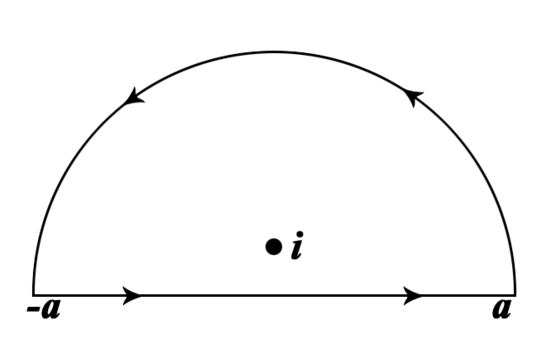
\includegraphics[scale=0.7]{contour}
	\caption{Wikipedia}
\end{figure}
in order to avoid integrating over some pole $z = i$.

\subsubsection{Cauchy Integral Formula}
In order to the perform the integral above in general, we can make use of something called the \textit{Cauchy integral formula}, which goes as follows. For any analytic function $f(z)$, if $z_0$ is interior to the contour $C$ then we have
\begin{align}
\boxed{f(z_0) = \f{1}{2\pi i}\int_C \f{f(z)}{z - z_0}\,dz}
\end{align}

which says that the values of $f$ inside the contour $C$ such that $\abs{z} = 2$ is determined by the value of $f$ on $C$. Let's use this to actually perform the integral. For example, say we would like to compute 
\begin{align}
\int_C \f{z\,dz}{(9-z^2)(z+i)} 
\end{align}
along a contour $C$ that contains only the \textit{pole} $z_0 = -i$. Then we first re-write the integral to match the Cauchy integral formula:
\begin{align}
\int_C \f{z\,dz}{(9-z^2)(z+i)} &= \int_C \f{1}{z+i}\lp \f{z}{9 - z^2} \rp\,dz
\end{align}
where $f(z)$ here is
\begin{align}
f(z) = \f{z}{9 - z^2}
\end{align}
which is analytic for $\abs{z} \leq 2$. By the integral formula, we have that
\begin{align}
\int_C \f{1}{z+i}\lp \f{z}{9 - z^2} \rp\,dz = f(z_0 = -i) = 2\pi i f(-i) = 2\pi i \f{-i}{9 + 1} = \f{\pi}{5}.
\end{align}

So believe it or not, we've just evaluated the integral without doing any integration!












\subsubsection{Taylor \& Laurent series}

Complex functions can have Taylor series or Laurent series, which is like Taylor series in a way except the powers are negative. 

\begin{figure}[!htb]
	\centering
	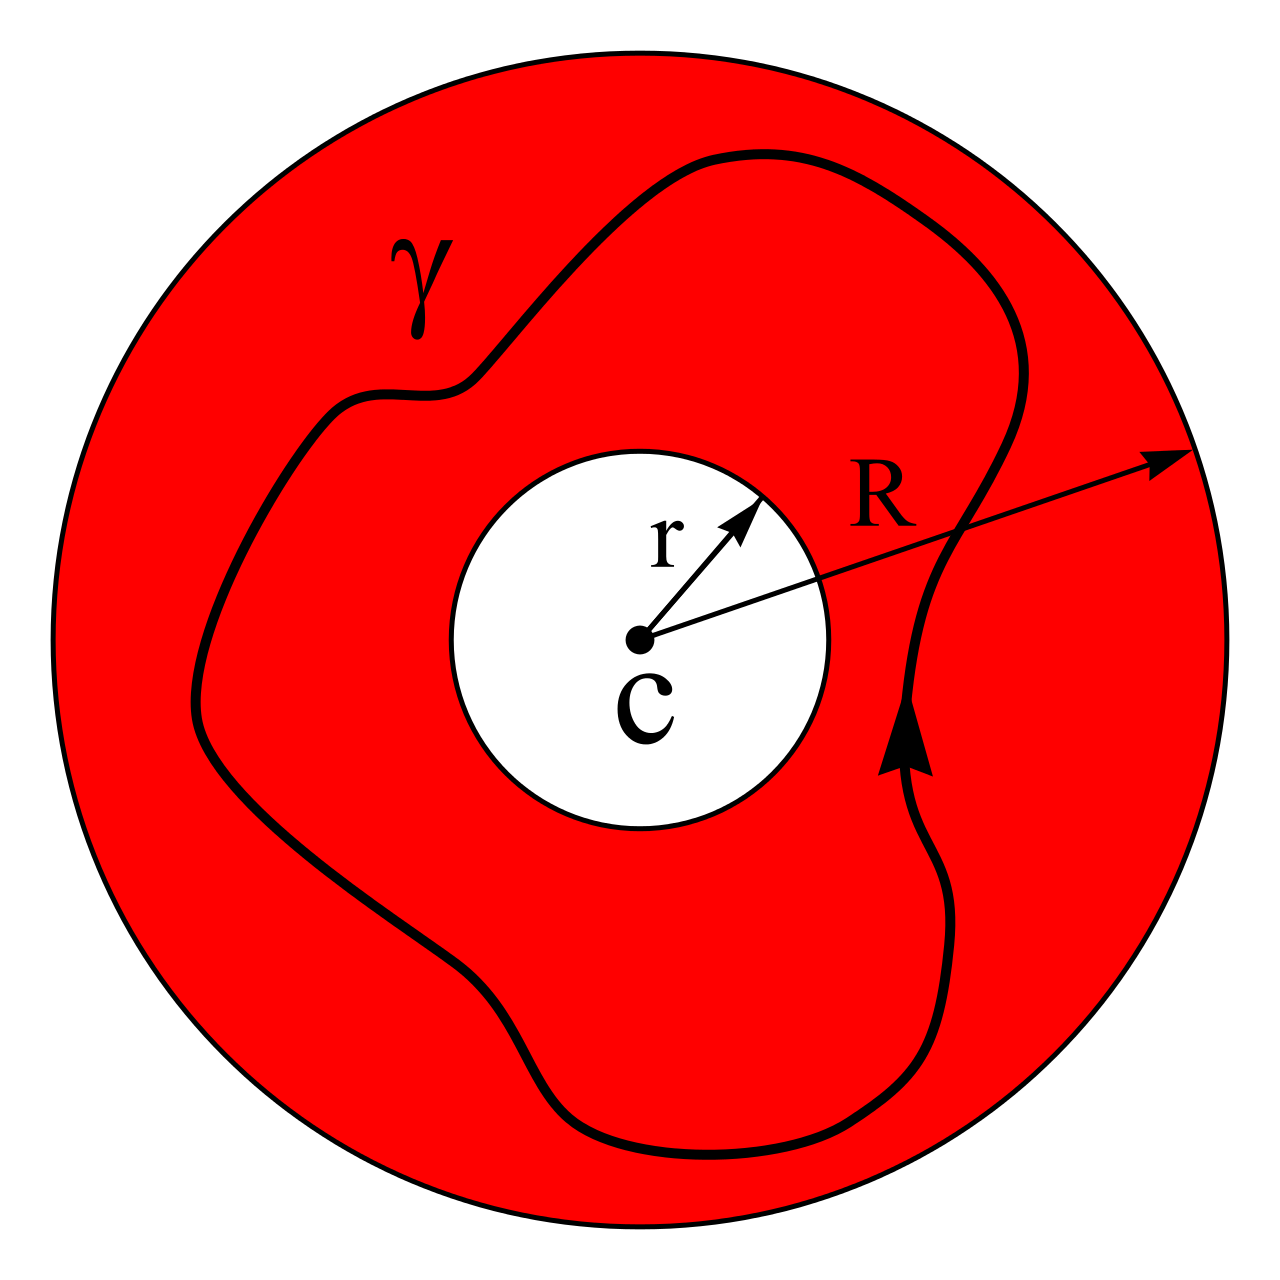
\includegraphics[scale=0.15]{laurent}
	\caption{Wikipedia}
\end{figure}

Let the contours $C_1$ and $C_2$ be concentric circles centered on $z_0$ with radii $r_1$ and $r_2$ where $r_2 < r_1$. Then we have a theorem which says if $f$ is analytic on $C_1$ and $C_2$ and everywhere in between then at each point $z$ in-between or on $C_1$ or $C_2$, we have
\begin{align}
\boxed{f(z) = \sum^\infty_{n=0}a_n (z - z_0)^n + \sum^\infty_{n=0}\f{b_n}{(z- z_0)^n}}
\end{align}
where
\begin{align}
a_n &= \f{1}{2\pi i }\int_{C_1} \f{f(s)\,ds}{(s - z_0)^{n+1}}\hspace{0.5cm} n = 0,1,2,3,\dots \\ 
b_n &= \f{1}{2\pi i }\int_{C_2} \f{f(s)\,ds}{(s - z_0)^{-n+1}}\hspace{0.5cm} n = 1,2,3,\dots
\end{align}
The series defined above is called the \textit{Laurent series} for $f$. \\

One thing we can do to recover a ``single'' contour $C$ is shrinking the inner radius $r_2 \to 0$, so that the domain becomes a punctured neighborhood of radius $r_1$ around $z_0$: $0 < \abs{z - z_0} < r_1$ and the $b_n$'s vanish.\\

If $f$ is analytic at all points inside and on $C_1$ then $f(z) / (z - z_0)^{-n+1}$ is also analytic since $-n+1 \leq 0$ and $b_n = 0$. This means the series reduces to a Taylor series. 











\subsubsection{The Residue Theorem}

A singular point of a function $f(z)$ is a point $z_0$ where $f$ is not analytic at $z_0$ but is analytic at every point in some neighborhood of $z_0$. So for example, the function $f(z) = 1/z$ is analytic everywhere except at $z=0$, so $z=0$ is a singular point. \\

Isolated singularities have neighborhoods around them on which $f$ is analytic. \\

When $f$ has an isolated singular point $z_0$, we define the \textit{residue} of $f$ at $z_0$ is the coefficient $b_1$ of its Laurent series:
\begin{align}
\boxed{b_1 = \f{1}{2\pi i}\int_{C} f(z)\,dz}
\end{align}

Note that the residue $b_1$ is the coefficient in the $1 / (z - z_0)$ term in the Laurent series:
\begin{align}
f(z) = \f{b_1}{z - z_0} + \dots
\end{align}


\textbf{The Residue Theorem:} Let $f$ be an analytic function in and on a closed contour $C$ except where it has singular points $z_1, z_2, \dots$ with corresponding residues $b_1, b_2, \dots$. Then 
\begin{align}
\boxed{\int_C f(z)\,dz = 2\pi i (b_1 + b_2 + \dots)}
\end{align}
i.e., the contour integral of $f$ around some contour $C$ which contains some of the singular points of $f$ is $2\pi i$ times the sum of the corresponding residues. \qed


For example, let's say we want to evaluate
\begin{align}
\int_C \f{5z - z}{z(z- 1)}\,dz
\end{align}
where the contour $C$ contains both the $0$ and $1$ poles. Then we first write the integrand so that it matches has the form of a Laurent series:
\begin{align}
\f{5z - 2}{z(z- 1)} = \f{1}{z}\lp \f{5z - 2}{z - 1} \rp = \f{1}{z-1}\lp\f{5z - 2}{z}\rp.
\end{align}
We find that the for the $z_0 = 0$ pole the residue is 
\begin{align}
b_1 = \f{0-2}{0-1} = 2.
\end{align}
For the $z_1 = 1$ pole the residue is
\begin{align}
b_2 = \f{5 - 2}{1} = 3.
\end{align}
So by the residue theorem,
\begin{align}
\int_C \f{5z - z}{z(z- 1)}\,dz = 2\pi i(2+3) = 10\pi i.
\end{align}


Let's do another example to get more comfortable. Suppose we want to evaluate
\begin{align}
\int_C \f{z^2}{1+z}\,dz
\end{align}
for a contour $C$ that contains the pole $z = -1$. For this pole, the corresponding residue is $(-1)^2 = 1$, so 
\begin{align}
\int_C \f{z^2}{1+z}\,dz = 2\pi i(1) = 2\pi i.
\end{align}

There are certainly techniques to evaluate integrals involving much more complicated poles, but we won't worry about that for now. 














\subsubsection{Evaluating real improper integrals}



One of many very nice applications of the residue theorem and the contour integrals is evaluating real improper integrals. Consider a general real improper integral 
\begin{align}
\int^{\infty}_{-\infty}f(x)\,dx
\end{align}
where $f$ now is a function that takes on real-valued arguments. If we extend $f$ over the complex plane and $f(z)$ has a pole at $z_0$ with positive imaginary part, then consider the contour with $\abs{z_0} < R$ which looks like the following
\begin{figure}
	\centering
	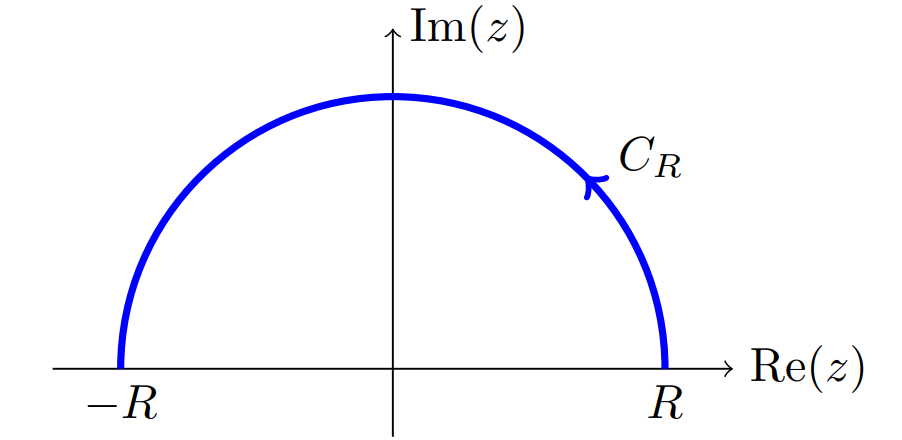
\includegraphics[scale=0.7]{improper}
\end{figure}
If 
\begin{align}
f(z) = \f{g(z)}{z - z_0}
\end{align}
then we have from the theorems
\begin{align}
\oint_C f(z)\,dz = 2\pi i g(z_0).
\end{align}
But we can also extend and make the contour very large by taking $R\to \infty$ since the contour integral stays the same
\begin{align}
\oint_C f(z)\,dz = \lim_{R\to \infty}\lp \int^R_{-R}f(x)\,dx + \int_{C_R}f(z)\,dz\rp
\end{align}
where the first term on the RHS is exactly the real improper integral we're looking for. Thus, so long as $f(z)$ on $C_R$ vanishes when we take $R\to \infty$, we must have that
\begin{align}
\boxed{\int^{\infty}_{-\infty}f(x)\,dx = 2\pi i g(z_0)}
\end{align}\qed



For example, let's say we want to evaluate the following integral
\begin{align}
\int^\infty_{-\infty} \f{2x^2 - 1}{x^4 + 5x^2 + 4}\,dx.
\end{align}

Well, while we can certainly try to do this completely on the real line, we can avoid the singularities by doing the contour integral. So let's write the integrand as
\begin{align}
f(z) = \f{2x^2 - 1}{(z^2 + 1)(z^2 + 4)}
\end{align}
which has poles at $z = \pm i, \pm 2i$. We also observe that for large $z$, $\abs{f(z)}\to 0$. This allows us to do use the contour integral. If we pick a contour that looks like a half-circle in the upper half plane with the base being the real axis, so that its radius is bigger than 2 (so that we can extend the contour to infinity), then we have, by what we've shown earlier
\begin{align}
\int_C f(z)\,dz = \int^\infty_{-\infty}f(x)\,dx + 0
\end{align}
where $0$ simply denotes the piece that vanishes when $R \to \infty$. With this, we move on to evaluating the contour integral. But notice that the contour includes only the $i$ and $2i$ poles, so we will only have two residues. Because we only have the $i$ and $2i$ poles, we write
\begin{align}
f(z) = \f{1}{z-i}\f{2z^2 - 1}{(z+i)(z^2 + 4)} = \f{1}{z - 2i}\f{2z^2 - 1}{(z^2 + 1)(z - 2i)}.
\end{align}
The residue that $z = i$ is then $i/2$, while the residue that $z = 2i$ is $-3i/4$. So the improper integral is
\begin{align}
\int^\infty_{-\infty} \f{2x^2 - 1}{x^4 + 5x^2 + 4}\,dx = 2\pi i\lp \f{i}{2} - \f{3i}{4} \rp = \f{\pi}{2}.
\end{align}










\newpage




\subsection{Multi-valued Functions \& Branch Cuts}



























\newpage




\subsection{From Field to Particle to Force}

Now that we've had the mathematical machinery in hand, we can tackle our worries about the $1/(k^2 - m^2)$ the keeps popping up in the integrals. \\

Let's start slow and try to evaluate the following integral
\begin{align}
\int^\infty_{-\infty} \f{dk}{k^2 - m^2}.
\end{align}

We obviously see that there are two poles $k =-m$ and $k = m$. While we will try to evaluate this using the a contour integral, it's not clear how we'll start because the poles are on the real axis. To resolve this slight issue, we will ``tilt'' the complex plane so that the ``poles'' are no longer on the real axis. \\

What we'll do is letting $m^2 \to m^2 - i\epsilon$ where $\epsilon > 0$ is some arbitrarily small positive number, just so we could push the pole a bit away from the real axis. Our goal is to evaluate the contour integral with $m^2 - i\epsilon$, then take the limit as $\epsilon\to \infty$ and hopefully get something finite. So, with $m^2 \to m^2 - i\epsilon$, we have
\begin{align}
k^2 - m^2 &\to k^2 - (m^2 - i\epsilon) \\ 
&= (k - \sqrt{m^2 - i\epsilon})(k + \sqrt{m^2 - i\epsilon}). 
\end{align}
Since $\epsilon$ can be chosen to be arbitrarily small, we will just do an expansion on the square root term without worrying to much
\begin{align}
\sqrt{m^2 - i\epsilon} &= m\sqrt{1 - \f{i\epsilon}{m^2}} \\ 
&\approx m - \f{i\epsilon}{2m} \\ 
&= m - i\epsilon' 
&\equiv m - i\epsilon
\end{align}
where we have let $\epsilon$ become the $\epsilon'$, which is something we can do because again $\epsilon$ can be chosen to be arbitrarily small. With this, we have
\begin{align}
k^2 - (m^2 - i\epsilon) = (k - (m - i\epsilon))(k + (m - i\epsilon)).
\end{align}

So now we have two poles at $k = m-i\epsilon$ and $k = -m + i\epsilon$, which are off the real axis. The next thing to do now is to evaluate the contour integral. We can make a closed contour using either the upper half-plane half-circle, or the lower half-plane half circle, each enclosing a different pole. 

\begin{figure}[!htb]
	\centering
	\includegraphics*[scale=0.1]{poles}
	\caption{Sketch by Prof. Robert Bluhm}
\end{figure}

Consider the contour integral on the left hand side. The enclosed pole here is $k = m - i\epsilon$. So to compute the residue we write
\begin{align}
\f{1}{k^2 - m^2 + i\epsilon} = \f{1}{k - (m - i\epsilon)}\f{1}{k + (m - i\epsilon)}.
\end{align}
The residue is therefore
\begin{align}
\f{1}{(m - i\epsilon) + (m - i\epsilon)} \to \f{1}{2m}
\end{align}
as we take $\epsilon \to 0$. If we consider the other contour then the residue is going to take on a minus sign, $-1/2m$. However, worry not, because the integrals over the real line in two contours have opposite directions. This means in either case, we get
\begin{align}
\int^\infty_{-\infty}\f{dk}{k^2 - m^2 + i\epsilon} = 2\pi i \lp \f{-1}{2m} \rp = \boxed{\f{-i\pi}{m}}.
\end{align}
Note that we can use the residue theorem to evaluate the integral here because as $k\to \infty, 1/(k^2 - m^2 + i\epsilon) \to 0$.

Okay, now suppose we want to evaluate something that is closer to what we're dealing with earlier:
\begin{align}
\int^\infty_{-\infty} \f{dk\, e^{ik(x-y)}}{k^2 - m^2 + i\epsilon}.
\end{align}

Consider the same two contours. We will see that both contours don't always work in both cases and whether the contour you choose works depends on whether $(x-y)$ is positive or negative. \\

Suppose $x - y > 0$. Then on $C_R$, we have that
\begin{align}
e^{iz(x-y)} \sim e^{i(iR)(x-y)} = e^{-R(x-y)} \to 0 \text{ as } R\to \infty,
\end{align}
where $iR$ represents the argument (up to phase shifts) that is fed into the exponent when integrating over the contour. On the other contour, however, because the argument now looks like $-iR$ times a phase factor, the sign of the exponent becomes positive, which means the function blows up. So, we see that the contour on the lower half-plane doesn't work when $x - y > 0$. The opposite happens when we have $x - y < 0$: only the contour on the lower half-plane works. \\

With this and the fact that the integrand still goes to zero as $k\to \infty$, we have for $x - y > 0$,
\begin{align}
\int^\infty_{-\infty} \f{dk\, e^{ik(x-y)}}{k^2 -m^2 + i\epsilon} = \int_C \f{dz \, e^{iz(x-y)}}{z^2 - m^2 + i\epsilon}.
\end{align}

So depending on the sign at $(x-y)$, we get combinations to the residue 
\begin{align}
\f{e^{2mi(x-y)}}{2m} \text{ or } \f{e^{-2mi(x-y)}}{-2m}
\end{align}
when $x - y>0$ and $x-y < 0$, respectively. \\

With this, we can now tackle the free theory propagator in QFT, which is given by
\begin{align}
\D(x-y) = \int \f{d^4 k }{(2\pi)^4} \f{e^{ik(x-y)}}{k^2 - m^2 + i\epsilon}
\end{align}

Here
\begin{align}
k^2 &= k_0^2 - \vec{k}^2 \\ 
d^4k &= dk_0\,d^3k
\end{align}
where we're using the conventional Minkowskian metric $\eta_{\mu\nu} = \text{diag}(1,-1,-1,-1)$. With this we rewrite the integral as
\begin{align}
\D(x-y) &= \f{1}{(2\pi)^4} \int^\infty_{-\infty}dk_0\,\int^\infty_{-\infty}d^3k\f{e^{ik_0(x^0 - y^0)}e^{-i\vec{k}\cdot(\vec{x} - \vec{y})}}{k_0^2 - (\vec{k}^2 + m^2) + i\epsilon},
\end{align}
where we don't really have to worry too much about $k^0$ or $k_0$ because of the metric. Now we'll call
\begin{align}
w_k^2 = \vec{k}^2 + m^2,
\end{align}
which the equivalent to the total energy. For the $k_0$ integration, which is an integration over time:
\begin{align}
k_0^2 - w_k^2 + i\epsilon = (k_0 - (w_k - i\epsilon))(k_0 + (w_k -i\epsilon))
\end{align}
and so we have poles at $k_0 = w_k - i\epsilon$ and $-w_k + i\epsilon$.\\

Once again, to perform this integral (correctly), we must pick the correct half-plane to close the contour. This choice depends on $x_0 - y_0$, which is the \textbf{time-ordering}. \\

It turns out that for $x^0 - y^0 >0$, we use the upper contour of radius $R$, where we have 
\begin{align}
e^{ik_0(x-y)} \sim e^{i(iR)(x^0-y^0)} = e^{-R(x^0-y^0)} \sim 0.
\end{align}
In this case, the pole is at $k_0 = -w_k + i\epsilon$. And so we can now evaluate the integral over all \textit{space} in the expression above:
\begin{align}
&\f{1}{(2\pi)^4}\int^\infty_{-\infty}d^3k\f{e^{ik_0(x^0 - y^0)}e^{-i\vec{k}\cdot(\vec{x} - \vec{y})}}{k_0^2 - (\vec{k}^2 + m^2) + i\epsilon}\\
= &\int \f{1}{k_0 + (w_k - i\epsilon)} \lp 
\f{d^3k}{(2\pi)^4}\f{e^{ik_0(x^0 - y^0)} e^{-i\vec{k}\cdot(\vec{x} - \vec{y})}}{k_0 - (w_k - i\epsilon)}
\rp.
\end{align}
Now, remember that this is our $f(k_0)$, and what we're actually trying to evaluate here is 
\begin{align}
\D(x-y) = \int dk^0 f(k_0).
\end{align}
By writing $f(k_0)$ as the triple integral over all \textit{space} like above, the residue is given by
\begin{align}
\int\f{d^3k}{(2\pi)^4}\f{e^{ik_0(x^0 - y^0)} e^{-i\vec{k}\cdot(\vec{x} - \vec{y})}}{k_0 - (w_k - i\epsilon)}
\end{align}
evaluated at the pole $k_0 = -w_k + i\epsilon$, taking $\epsilon \to 0$. The value of this at $k_0 = -w_k +i\epsilon$ as $\epsilon\to 0$ is
\begin{align}
&\int \f{d^3k}{(2\pi)^4} \f{e^{-iw_k(x^0 - y^0)}e^{-i\vec{k}\cdot (\vec{x} - \vec{y})}}{-w_k - w_k} \\ 
= &\int \f{d^3k}{(2\pi)^4} \f{e^{-iw_k(x^0 - y^0)}e^{-i\vec{k}\cdot (\vec{x} - \vec{y})}}{-2w_k}.
\end{align}
This is the residue. And so the value of the propagator is then
\begin{align}
\D(x-y) = \int dk^0 \,f(k_0) = 2\pi i \lb \int \f{d^3k}{(2\pi)^4} \f{e^{-iw_k(x^0 - y^0)}e^{-i\vec{k}\cdot (\vec{x} - \vec{y})}}{-2w_k} \rb. 
\end{align}
So,
\begin{align}
\D(x-y) = \f{1}{(2\pi)^3} \int \f{-i}{2w_k}d^3k\,e^{-i[w_k(x^0 - y^0) + \vec{k}\cdot(\vec{x} - \vec{y})]}
\end{align}

On the other hand, if $x^0 - y^0 <0$, then we would use the other pole and close the contour in the lower half-plane to get
\begin{align}
\D(x-y) &= -2\pi i\f{1}{(2\pi)^4}\int d^3k\, \f{e^{iw_k(x^0 - y^0)}e^{-i\vec{k}\cdot(\vec{x} - \vec{y})}}{2w_k} \\ 
&= \f{1}{(2\pi)^3}\int  \f{-i}{2w_k} d^3k\,e^{iw_k(x^0 - y^0)}e^{-i\vec{k}\cdot(\vec{x} - \vec{y})}  \\
&= \boxed{\f{1}{(2\pi)^3}\int \f{-i}{2w_k}d^3k\,e^{i[w_k(x^0 - y^0) - \vec{k}\cdot(\vec{x} - \vec{y})]}}
\end{align}
where the minus sign comes from integrating over the real line in the $(-)$ direction. The pole is now $k_0 = w_k - i\epsilon$ and the residue is
\begin{align}
\f{1}{(2\pi)^3}\int d^3k\, \f{e^{iw_k(x^0 - y^0)}e^{-i\vec{k}\cdot(\vec{x} - \vec{y})}}{2w_k}
\end{align}
when $\epsilon \to 0$.\\

We see that the expression for the propagator when $x^0 - y^0 > 0$ and $x^0 - y^0 < 0$ differ by a little bit in the sign of $\vec{k}$ in the factor inside the exponent. However, we note that because of symmetry, by letting $\vec{k} \to -\vec{k}$ in the $x^0 - y^0 > 0$ case and using symmetry:
\begin{align}
\int d^3k = \int d^3(-\vec{k})
\end{align}
we can re-write:
\begin{align}
{\D(x-y) = \f{1}{(2\pi)^3} \int \f{-i}{2w_k}d^3k\,e^{-i[w_k(x^0 - y^0) - \vec{k}\cdot(\vec{x} - \vec{y})]}}
\end{align} 
for the $x^0 - y^0 > 0$ case. \\

The next thing we want to do is combining the two propagators into a single expression. This requires having a function that specifies the correct sign of $x^0 - y^0$, which is exactly what the Heaviside step function does. Define
\begin{align}
\theta = \begin{cases}
1 \hspace{0.5cm} x^0 - y^0 > 0\\ 
0 \hspace{0.5cm} x^0 - y^0 < 0
\end{cases}
\end{align}
where we will take $\theta = 1/2$ if $x^0 = y^0$.\\


With this and taking $y = 0$ to be the initial spacetime and $x^0 = t$,  we can write the propagator as
\begin{align}\label{propag}
\boxed{\D(x) = \f{-i}{(2\pi)^3}\int \f{d^3k}{ 2 w_k} \lb e^{-i[w_kt - \vec{k}\cdot\vec{x}]}\theta(t) + e^{i[w_kt - \vec{k}\cdot\vec{x} ]}\theta(-t)\rb}
\end{align}

Let us note a few things here before moving on. For spacelike $x$, i.e., $x = (t,\vec{x}) = (t,0)$, we have that if $t >0$ (in the future cone), the propagator has the form
\begin{align}
\D(x) = \f{-i}{(2\pi)^3}\int \f{d^3k}{2 w_k}e^{-iw_kt}.
\end{align}
This says the propagator is a superposition of plane waves and oscillates. Similar with the past cone where $t<0$, $\D$ also oscillates but with a different phase ($e^{iw_kt}$). \\

For timelike $x$, i.e., $x = (0,\vec{x})$, we have that 
\begin{align}
\D(x) = \f{-i}{(2\pi)^3}\int \f{d^3k}{ 2 w_k}e^{-i\vec{k}\cdot\vec{x}} =\f{-i}{(2\pi)^3}\int \f{d^3k}{ 2 \sqrt{\vec{k}^2 + m^2}}e^{-i\vec{k}\cdot\vec{x}} .
\end{align}
where we have flipped the sign of $\vec{k}$ again to cancel the factor of $1/2$. \textit{In order to evaluate this integral, we will need to understand \textbf{branch cuts}, which we will cover later. }






































\newpage





\subsection{From field to particle}

Recall that from free scalar with source $J(x)$ we have obtained a functional $W(J)$:
\begin{align}
W(J) = -\f{1}{2}\iint d^4xd^4y\, J(x)\D(x-y)J(y)
\end{align}
where $W(J)$ is called the generating function for connected diagrams, and $\D(x-y)$ is basically the Green's function which carries the effects of the source at $y$ to $x$. \\


In terms of the Fourier transform 
\begin{align}
J(x) &\equiv  \F^{-1}[J(k)](x) = \int d^4x \, J(k)e^{-ikx}\\
\D(x-y) &\equiv \f{1}{(2\pi)^4}\int d^4k\,\f{1}{k^2 - m^2}e^{ik(x-y)}
\end{align}
So we have
\begin{align}
W(J) = -\f{1}{2}\f{1}{(2\pi)^4}\int d^4k\, J(k)^* \f{1}{k^2 - m^2 + i\epsilon}J(k) 
\end{align}
where we have taken the complex conjugate of $J(x)$ to get the correct Fourier transform.  \\

Now, consider the case where we have two sources $J_1, J_2$ in spacetime such that $J(x) = J_1(x) + J_2(x)$
\begin{figure}[!htb]
	\centering
	\includegraphics*[scale=0.7]{source}
	\caption{From Zee}
\end{figure}
Then $W(J)$ contains four terms involving $J_1$ and $J_2$. One of the terms contains $J_2^* J_1$:
\begin{align}
W(J) = -\f{1}{2}\int \f{d^4k}{(2\pi)^4} J_2^*(k)\f{1}{k^2 - m^2 + i\epsilon} J_1(k).
\end{align} 

We interpret this as follows: in region 1 in spacetime there is a source that sends out some disturbance in the field, which is then absorbed by a sink in region 2 in spacetime. \\

When $k^2 = m^2$, $k$ is said to be on mass shell. For arbitrary $k$, it is a linguistic convenience to say that a``virtual particle'' of momentum $k$ propagates from
the source to the sink.











\subsubsection{Particle to force}


Consider the same source $J = J_1 + J_2$ again and consider the $W(J)$, neglecting the $J_1^*J_1$ and $J_2^*J_2$ self-interactions. And suppose that 
\begin{align}
J_a(\vec{x}) = \delta^{(3)}(\vec{x} - \vec{x}_a).
\end{align}
Note that $J$ is real and so we will get a factor of $2$ when obtaining $W(J)$. \\

Plugging everything into 
\begin{align}
W(J) = -\f{1}{2}\iint d^4xd^4y\, J(x)\D(x-y)J(y).
\end{align}
we obtain (remember the factor of 2...)
\begin{align}
W(J) &= -\f{2}{2}\iint dx^0 dy^0 \int \f{d^0k}{2\pi} e^{ik^0(x-y)^0} \int \f{d^3k }{(2\pi)^3} \f{e^{i\vec{k}\cdot (\vec{x}_1 - \vec{x}_2)}}{k^2 - m^2 + i\epsilon}\\
&= -\iint dx^0 dy^0 \int \f{d^0k}{2\pi} e^{ik^0(x-y)^0} \int \f{d^3k }{(2\pi)^3} \f{e^{i\vec{k}\cdot (\vec{x}_1 - \vec{x}_2)}}{k^2 - m^2 + i\epsilon}
\end{align}
where the piece
\begin{align}
2\int \f{d^0k}{2\pi} e^{ik^0(x-y)^0}
\end{align}
comes from the transforms of the source delta functions and the piece
\begin{align}
\f{e^{i\vec{k}\cdot (\vec{x}_1 - \vec{x}_2)}}{k^2 - m^2 + i\epsilon} \\
\end{align} 
comes from the transform of the propagator $\D(x-y)$. \\

Next, integrating over all $y^0$ and absorbing the delta-function-transform piece give us a delta function, which sets $k^0$ to zero. As a result,
\begin{align}
k^2 = k^0 - \vec{k}^2 = \vec{k}^2
\end{align}
So that $W(J)$ becomes
\begin{align}
W(J) = \lp \int dx^0 \rp \int \f{d^3x}{(2\pi)^3} \f{e^{i\vec{k}\cdot (\vec{x}_1 - \vec{x}_2)}}{\vec{k}^2 + m^2}
\end{align}
where we have dropped $i\epsilon$ because the denominator is can no longer be zero.   \\

Next, recall the \textbf{generating function} we have defined previously
\begin{align}
\mathcal{Z} = \zeta e^{iW(J)} \sim \bra{0}e^{-iHT}\ket{0} = e^{-iET}
\end{align} 
where
\begin{align}
T = \int dx^0
\end{align}
is the time interval. So we have 
\begin{align}
\boxed{E = -\int \f{d^3k}{(2\pi)^3}\f{e^{i\vec{k}\cdot(\vec{x}_1 - \vec{x}_2)}}{\vec{k}^2 + m^2}}
\end{align}
Let us evaluate this integral. First, we write 
\begin{align}
\vec{x} &= \vec{x}_1 - \vec{x}_2 \\ 
u &\equiv \cos\theta = (\vec{k},\vec{x}).
\end{align}
In spherical coordinates where
\begin{align}
k &= \abs{\vec{k}} \\
r &= \abs{\vec{x}},
\end{align}
we have the volume element is
\begin{align}
d^3k = k^2 \sin \theta \,dk,d\theta\,d\phi = -  k^2 \, d(\cos\theta)\,d\phi.
\end{align}
But notice that even though we get an extra minus sign, the integration bounds also flips accordingly, so the overall sign of the integral doesn't chance. Thus,
\begin{align}\label{inverse-sq}
E &= -\int \f{d^3k}{(2\pi)^3}\f{e^{i\vec{k}\cdot(\vec{x}_1 - \vec{x}_2)}}{\vec{k}^2 + m^2} \nonumber\\
&= -\f{1}{(2\pi)^3}\int_0^{2\pi}d\phi\,\int^\infty_0 dk\,k^2 \int^{1}_{-1}d(\cos\theta)\f{e^{ikx\cos\theta}}{k^2 + m^2} \nonumber\\
&= -\f{1}{(2\pi)^2}\int^\infty_0 dk\,k^2 \int^{1}_{-1}du\,\f{e^{ikru}}{k^2 + m^2} \nonumber\\
&= -\f{1}{(2\pi)^2} \int^\infty_0 dk\,\f{1}{k^2 + m^2} \lp \f{1}{ikr}e^{ikru} \rp\bigg\vert^1_{-1}\nonumber\\
&= -\f{1}{(2\pi)^2} \int^\infty_0 dk\,\f{1}{k^2 + m^2} \lb \f{2i}{ikr}\sin(kr)\rb\nonumber\\
&= -\f{2i}{(2\pi)^2ir} \int^\infty_0 dk\,\f{k\sin (kr)}{k^2 + m^2}\nonumber\\
&= -\f{1}{(2\pi)^2r} \int^\infty_{-\infty}dk\,\f{k\sin (kr)}{k^2 + m^2} \hspace{0.5cm} \text{(even integrand)}\nonumber\\
&= -\f{1}{(2\pi)^2r} \int^\infty_{-\infty}dk\,\lp\f{1}{k - im}\rp\f{k\sin(kr)}{k + im}\nonumber\\
&= -\f{1}{(2\pi)^2r}\int^\infty_{-\infty}dk\,\lp\f{1}{k - im}\rp\f{1}{2i}\f{k(e^{ikr} - e^{-ikr})}{k + im} \nonumber\\
&= -\f{1}{(2\pi)^2r}\int^\infty_{-\infty}dk\,\lp\f{1}{k - im}\rp\f{1}{2i}\f{k(e^{ikr} + e^{ikr})}{k + im}\nonumber\\
&=  -\f{1}{(2\pi)^2r}\int^\infty_{-\infty}dk\,\lp\f{1}{k - im}\rp\f{1}{i}\f{k e^{ikr}}{k + im}\nonumber\\
&= -\f{1}{(2\pi)^2ri}\int^\infty_{-\infty}dk\,\lp\f{1}{k - im}\rp\f{k e^{ikr}}{k + im}\nonumber \\
&= -\f{1}{(2\pi)^2ri}\int_{C}dk\,\lp\f{1}{k - im}\rp\f{k e^{ikr}}{k + im} \hspace{0.5cm} \text{*contour around } im \nonumber\\
&= -\f{1}{(2\pi)^2ri}(2\pi i)\f{im e^{i(+im)r}}{im + im} \nonumber\\
&= \boxed{-\f{1}{4\pi r}e^{-mr}}
\end{align}

Thus the energy is \textbf{negative}, which means the two delta function sources give an attractive force. We identify $E$ as the potential energy between two static sources. We also note the range of the attractive force generated by the field $\psi$ is determined inversely by the mass $m$ of the particle. Does this sound familiar?????















\subsubsection{The Origin of Force}

We now see that the exchange of particle (via $\D$) can produce a force, which is given by the potential. We can associate a particle with each of the known forces: photon with the electromagnetic force, graviton with gravity(?). \\

More importantly, however, we see where the \textbf{inverse square law} comes from, based on the form of the potential. We notice that if the force-carrying particle has mass 0 (which is the case for photon in electromagnetism and graviton in gravitation) then the potential energy has the form
\begin{align}
E = \f{1}{4\pi r}.
\end{align}
The gradient of this gives the force, which is proportional to $1/r^2$. \\

Where does this come from? The answer can be traced all the way back to the Lagrangian density for the simplest field theory where we have $\p_\mu$ and $\p^\mu$, i.e., two powers of the spacetime derivative. This ensures Lorentz invariance. 












\subsubsection{Connected versus disconnected}

We might want to represent the integrand
\begin{align}
J(x)\D(x-y)J(y)
\end{align}
as a connected path in $W(J)$ to present a disturbance from $y$ to $x$. This is the beginning of Feynman diagrams. 
\begin{figure}[!htb]
	\centering
	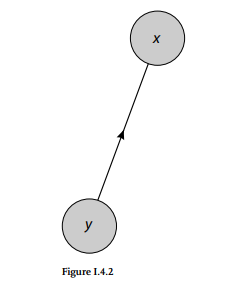
\includegraphics[scale=0.7]{feynman-1}
	\caption{From Zee}
\end{figure}

Next, recall the definition of the generation function $\mathcal{Z}$:
\begin{align}
\boxed{\mathcal{Z}(J) = \mathcal{Z}(0)e^{iW(J)} = \mathcal{Z}(J=0)\sum^\infty_{n=0}\f{[iW(J)]^n}{n!}}
\end{align}
The $n=2$ term is given by
\begin{align}
\f{1}{2!}\lp -\f{i}{2} \rp^2 \iiiint d^4x_1d^4x_2d^4x_3d^4x_4\D(x_1 - x_2)\D(x_3 - x_4)J(x_1)J(x_2)J(x_3)J(x_4).
\end{align}
The integrand is given by
\begin{figure}[!htb]
	\centering
	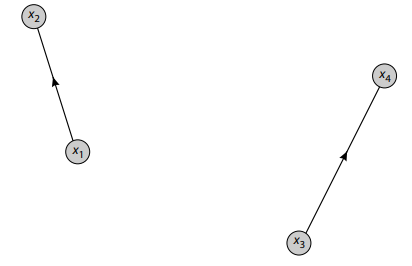
\includegraphics[scale=0.6]{feynman-2}
	\caption{From Zee}
\end{figure}
We see this is the correct figure because the $1\to 2$ propagation is independent of $3\to 4$. 




















\subsubsection{Like charges repel}

Quantum field theory of electromagnetism is called quantum electrodynamics, or QED for short. For this section we will consider the theory of a massive spin 1 vector. We will assume that the photon mass is nonzero, only to plug in $m=0$ in the end to see if things are okay. \\

Recall the Lagrangian:
\begin{align}
\lag = -\f{1}{4}F_{\mu\nu}F^{\mu\nu}
\end{align}
where
\begin{align}
F_{\mu\nu} = \p_\mu A_\nu - \p_\nu A_\mu
\end{align}
where $A_\mu(x)$ is the vector potential. With our assumption that the mass of the photon is nonzero, we will introduce both a mass term and a source term to the Lagrangian, which then becomes
\begin{align}
\lag = -\f{1}{4}F_{\mu\nu}F^{\mu\nu} + \f{1}{2}m^2A_\mu A^\mu + A_\mu J^\mu.
\end{align}
Note that the source here is a just a current, which satisfied the conservation law:
\begin{align}
\p_\mu J^\mu = 0.
\end{align}
The path integral of this theory is
\begin{align}
\Z = \int \mathfrak{D} \,Ae^{iS[A]} = e^{iW(J)}
\end{align}
where the functional action in terms of the vector potential
\begin{align}
S[A] = \int d^4x\,\lag &= \int d^4x \lb -\f{1}{4}F_{\mu\nu}F^{\mu\nu} + \f{1}{2}m^2A_\mu A^\mu + A_\mu J^\mu \rb \\ 
&= \int d^4x\,\lb \f{1}{2}A_\mu \lb (\p^2 + m^2)g^{\mu\nu} - \p^\mu \p^\nu \rb A_\nu + A_\mu J^\mu  \rb
\end{align}
where the second equality comes from integration by parts. Now, just like when we were dealing with the free scalar field with source, we want the propagator $\D$ to be the inverse of the differential operator, i.e.,
\begin{align}
\lb (\p^2 + m^2)g^{\mu\nu} - \p^\mu \p^\nu \rb \D_{\nu\lambda}(x) = \delta^\mu_\lambda \delta^{(4)}(x).
\end{align}
Just like before, by going into momentum space we can extract the wave vector $k$ from the differential operator. To do this, we will have to go way back to the beginning of this section, Fourier transform everything and putting everything back into a original equation. The propagator in position space is related to the propagator in momentum space by
\begin{align}
\D{\nu\lambda}(x) = \F[\D(k)](x) = \int \f{d^4k}{(2\pi)^4} D_{\nu\lambda}(k)e^{ik(x)}.
\end{align}
Plugging this back into our equation and writing the delta function as a Fourier transform to get
\begin{align}
\int \f{d^4k}{(2\pi)^4}D_{\nu\lambda}(k) \lb (\p^2 + m^2)g^{\mu\nu} - \p^\mu \p^\nu \rb e^{ikx} = \delta^\mu_\lambda \int \f{d^4k}{(2\pi)^4}e^{ikx}.
\end{align}
Letting the differential operator act on $e^{ikx}$
\begin{align}
\int \f{d^4k}{(2\pi)^4}D_{\nu\lambda}(k) \lb -(k^2 - m^2)g^{\mu\nu} + k^\mu k^\nu \rb e^{ikx} = \delta^\mu_\lambda \int \f{d^4k}{(2\pi)^4}e^{ik(x)}.
\end{align}
And so it must follow that
\begin{align}
\lb -(k^2 - m^2)g^{\mu\nu} + k^\mu k^\nu \rb \D_{\nu\lambda}(k) = \delta^{\mu}_\lambda
\end{align}
Solving for the propagator, we get
\begin{align}
\boxed{D_{\nu\lambda}(k) = \f{-g_{\nu\lambda} + k_\nu k_\lambda / m^2}{k^2 - m^2}}
\end{align}
This is the \textbf{masive vector meson propagator}, or the photon propagator loosely speaking. With this, we can now write the generating function for connected diagrams as
\begin{align}
W(J) = -\f{1}{2}\int \f{d^4k}{(2\pi)^4}J^\mu(k)^*\f{-g_{\nu\lambda} + k_\nu k_\lambda / m^2}{k^2 - m^2 + i\epsilon} J^\nu(k)
\end{align}
where the $i\epsilon$ is added to the denominator because (as you can tell this is coming) we will need to do a contour integral around a pole to get a finite answer. \\

We also have that the conservative of current $\p_\mu J^\mu = 0$ in momentum space becomes $k_\mu J^\mu = 0$, this means the $k_\mu k_\nu$ term in the numerator gets killed by the $J's$. We also have that $g_{\mu\nu} \sim 1$, so effectively the generating function is 
\begin{align}
W(J) \sim \f{1}{2}\int \f{d^4k}{(2\pi)^4}J^\mu(k)^*\f{1}{k^2 - m^2 + i\epsilon} J^\nu(k)
\end{align}
where the minus sign disappears. So, by comparing this result to what we have found in the previous section, we see that the energy obtained is positive so long as the charge densities $J$'s have the same sign. This basically says like charges repel. \\

With this, no more computation is needed. With
\begin{align}
E = \f{1}{4\pi r}e^{-mr},
\end{align} 
we simply let the photon mass go to zero to get
\begin{align}
E \to \f{1}{4\pi r}.
\end{align}
This is exactly the form of the electric potential in electrostatics.







\subsubsection{Planck Mass}

The Planck Mass, denoted $M_{Pl}$ is defined in terms of the Newton's law of gravity:
\begin{align}
V(r) = \f{G_N m_1 m_2}{r} = \f{m_1 m_1}{M^2_{Pl}} \lp \f{1}{r}\rp.
\end{align}
Numerically, 
\begin{align}
M_{Pl} \approx 10^{19} \text{ GeV}.
\end{align}
It is clear why gravity is so weak compared to, say, the electromagnetic force. 







\newpage


\subsection{Feynman Diagrams}







\subsubsection{Gaussian Integrals and their Moments}


Before getting into how trying to evaluate these integrals gives us Feynman diagrams, we should quickly revisit Gaussian integrals, as they are \textit{very} similar to many integrals in QFT.\\

The first basic result is the following:
\begin{align}
I = \int_\mathbb{R}dx\, e^{-x^2} = \sqrt{\pi}.
\end{align}
A very clever way to do this is to move to the two dimensional case and try to evaluate
\begin{align}
I^2 = \int_{\mathbb{R}^2} dxdy\, e^{-x^2 - y^2}.
\end{align}
We can move into polar coordinates and do a change of variables to get
\begin{align}
I^2 = \int_0^\infty (2\pi) rdr\,e^{-r^2}.
\end{align}
We can evaluate this integral with a $u$-substitution. to get
\begin{align}
I^2 = 2\pi \f{1}{2} = \pi \implies I = \sqrt{\pi}.
\end{align}
In general,
\begin{align}
\boxed{\int_\mathbb{R} dx\, \exp\lp -\f{a}{2}x^2 + bx \rp = \sqrt{\f{2\pi}{a}} \exp\lp \f{b^2}{2a} \rp }
\end{align}
We do this by completing the square then rescaling and shifting the integration variables. (This is why we have a left over exponent in the end.)\\

The next things we want to evaluate are various moments of the Gaussian, i.e., integrals like
\begin{align}
I_n = \int_\mathbb{R} dx\, x^n \exp\lp -\f{a}{2}x^2 \rp.
\end{align}
We assume that $n$ is a positive integer. If $n$ is odd then the integrand is an odd function, so when it is integrated over a symmetric domain we get 0. On the other hand, when $n$ is even, we use Feynman's \textbf{differentiating-under-the-integral-sign} trick. Here is how it works:\\


\textbf{Feynman's integration technique:} Consider the previous integral:
\begin{align}
\int_\mathbb{R} dx\, \exp\lp -\f{a}{2}x^2 + bx \rp.
\end{align}  
We notice that when we take the derivative of the integrand with respect to $b$ we bring down a factor of $x$:
\begin{align}
\f{d}{db}\, \exp\lp -\f{a}{2}x^2 + bx \rp = x\exp\lp -\f{a}{2}x^2 + bx \rp.
\end{align}
So, in order to get $x^n$ in the integrand of the integral
\begin{align}
I_n = \int_\mathbb{R} dx\, x^n \exp\lp -\f{a}{2}x^2 \rp,
\end{align}
we will take $\p_b$ of the other integrand $n$ times to bring down $x^n$ then set $b = 0$. Let's do this:
\begin{align}
\lp\f{d}{db}\rp^n \exp\lp -\f{a}{2}x^2 + bx \rp \bigg\vert_{b=0} = x^n \exp\lp -\f{a}{2}x^2 + bx \rp\bigg\vert_{b=0} = x^n \exp\lp -\f{a}{2}x^2\rp,
\end{align}
which is exactly what we wanted. Okay, but we still haven't successfully evaluated the integral yet. To do this, we will look at the original ``guiding'' equation again:
\begin{align}
\int_\mathbb{R} dx\, \exp\lp -\f{a}{2}x^2 + bx \rp = \sqrt{\f{2\pi}{a}} \exp\lp \f{b^2}{2a} \rp.
\end{align}
Differentiate wrt $b$ $n$ times and setting $b = 0$ in the end gives
\begin{align}
\lp\f{d}{db}\rp^n \int_\mathbb{R} dx\, \exp\lp -\f{a}{2}x^2 + bx \rp \bigg\vert_{b=0} 
&= \sqrt{\f{2\pi}{a}}\lp\f{d}{db}\rp^n \exp\lp \f{b^2}{2a} \rp\bigg\vert_{b=0} \nonumber \\
\int_\mathbb{R}\lp\f{d}{db}\rp^n  dx\, \exp\lp -\f{a}{2}x^2 + bx \rp\bigg\vert_{b=0} 
&= \sqrt{\f{2\pi}{a}}\lp\f{d}{db}\rp^n \exp\lp \f{b^2}{2a} \rp\bigg\vert_{b=0}.
\end{align}
Therefore,
\begin{align}
\boxed{\int_\mathbb{R}dx\, x^n \exp\lp -\f{a}{2}x^2\rp 
= \sqrt{\f{2\pi}{a}}\f{n!}{(n/2)!(2a)^{n/2}}}
\end{align}
Note that $n$ here is even. If $n$ is odd then the integral is zero. Next, to correctly normalize these integrals, we can find the normalization factor simply by
\begin{align}
\boxed{\f{\int_\mathbb{R}dx\, x^n \exp\lp -\f{a}{2}x^2\rp }{\int_\mathbb{R}dx\, \exp\lp -\f{a}{2}x^2\rp } = \f{n!}{(n/2)!(2a)^{n/2}}}
\end{align}
These higher moments of the Gaussian are called the \textbf{correlation functions}. 	 \\

So how are these higher moments related to Feynman diagrams? The answer is given by the combinatoric interpretation of values of the integrals. Suppose we would like make ($n/2$) pairs from $n$ distinguishable things. The answer is 
\begin{align}
{ n \choose n}{n-2 \choose 2}\dots {2 \choose 2} \times \f{1}{(n/2)!} = \f{n!}{2^{n/2}(n/2)!}.
\end{align}
This is not so different from what we just found, except the factor of $1/a$. This is where the physics come in. Observe that if we add in a weight factor of $1/a$ each time we make a pair then we get the same thing from the integral. These factors of $1/a$ are the \textbf{propagators}! 









\subsubsection{Anharmonicity in field theory}

So far, integrals in free field theory have been Gaussian, meaning we can evaluate them one way or the other using the prescription laid out above. However, particles don't interact in this theory because we don't have ``anharmonic'' in the Lagrangian (these make the equation of motion no longer linear). \\

Revisit the combinator interpretation of the values of the integrals above. If we associate to each pair of the $n$ things an \textit{edge} connecting them, then we see when things are alreay in pairs they don't interact with our future choices. This is quite hand-wavy, but the idea is that if the exponent inside the integrand is quadratic (or can be square-completed) then we can evaluate things exactly. But what if there are higher order terms, or alternatively \textit{anharmonic} terms? \\

Suppose we add only one anharmonic term $-(\lambda / 4!)\phi^4$ to our free field theory and try to evaluate
\begin{align}
\Z(J) = \int \mathfrak{D}\phi \exp\lp i\int d^4x\,  \f{1}{2}\lb(\p \phi)^2 - m^2 \phi^2 \rb - \f{\lambda}{4!}\phi^4 + J(x)\phi \rp.
\end{align}
This isn't so doable anymore! It's possible, but imagine adding higher order terms to the Lagrangian! 











\subsubsection{Feynman diagrams: A baby problem}

Let us try to evaluate a simpler version of the integral above:
\begin{align}
\Z(J) = \int^\infty_{-\infty} dq\, \exp\lp -\f{1}{2}m^2 q^2 - \f{\lambda}{4!}q^4 + Jq \rp.
\end{align}

Here we don't have a nice trick to complete the square. However, we can use the exact result obtained earlier with the higher order moments of the Gaussian integral to try to approximate this integral. The idea is to Taylor expand the higher order term and turn it into a polynomial in $q^4$ when appropriate:
\begin{align}
\exp\lp -\f{1}{2!}\f{\lambda}{4!}q^4 \rp = 1 - \lp\f{\lambda}{4!}\rp q^4 + \f{1}{2!}\lp\f{\lambda}{4!}\rp^2 q^8 - \dots
\end{align}
With this, we get
\begin{align}
\Z(J) = \int^\infty_{-\infty} dq\,  \lb 1 - \lp\f{\lambda}{4!}\rp q^4 + \f{1}{2!}\lp\f{\lambda}{4!}\rp^2 q^8 - \dots \rb e^{ -\f{1}{2}m^2 q^2 + Jq }.
\end{align}

Then, we \textit{simply} integrate term-by term. This we can do because now they are just $q^{4n}$ moments of the original Gaussian, i.e., each term has the form
\begin{align}
\int_\mathbb{R} dq\, e^{(-1/2)m^2 q^2 + Jq}q^{4n}.
\end{align}
To bring down a factor of $q^{4n}$ for each term we have to differentiate wrt $J$ $4n$ times:
\begin{align}
\int_\mathbb{R} dq\, e^{(-1/2)m^2 q^2 + Jq}q^{4n} &= \int_\mathbb{R}\,dq \lp \f{d}{dJ} \rp^{4n} e^{(-1/2)m^2 q^2 + Jq} \\
&=   \lp \f{d}{dJ} \rp^{4n} \int_\mathbb{R}dq \, e^{(-1/2)m^2 q^2 + Jq}.
\end{align}

Because $\Z(J)$ is a sum of such terms, we get
\begin{align}
\boxed{\Z(J) = \lb 1 - \lp\f{\lambda}{4!}\rp \f{d^4}{dJ^4} + \f{1}{2!}\lp\f{\lambda}{4!}\rp^2 \f{d^8}{dJ^8} - \dots \rb\int_\mathbb{R}dq \, e^{(-1/2)m^2 q^2 + Jq}}
\end{align}

But that's not all, observe that we have just replaced 
\begin{align}
q^{4n} \to \f{d^{4n}}{dJ^{4n}}.
\end{align}

So it only makes sense that we write 
\begin{align}
\exp\lb -\f{\lambda}{4!}\lp \f{d}{dJ} \rp^4 \rb = \lb 1 - \lp\f{\lambda}{4!}\rp \f{d^4}{dJ^4} + \f{1}{2!}\lp\f{\lambda}{4!}\rp^2 \f{d^8}{dJ^8} - \dots \rb.
\end{align}
We also know how to evaluate the leftover integral by completing the squares. So, 
\begin{align}
\int_\mathbb{R}dq \, e^{(-1/2)m^2 q^2 + Jq} = \sqrt{\f{2\pi}{m^2}}\exp\lp \f{J^2}{2m^2} \rp.
\end{align}

Thus we have successfully evaluated $\Z(J)$:
\begin{align}
\boxed{\Z(J) = \exp\lb -\f{\lambda}{4!}\lp \f{d}{dJ} \rp^4 \rb \sqrt{\f{2\pi}{m^2}}\exp\lp \f{J^2}{2m^2} \rp = \sqrt{\f{2\pi}{m^2}} e^{-\f{\lambda}{4!}\lp \f{d}{dJ} \rp^4} e^\f{J^2}{2m^2}}
\end{align}

From now on, we will let 
\begin{align}
\Z(J=0, \lambda =0) = \sqrt{2\pi / m^2} \equiv \Z(0,0)
\end{align}
We will also define
\begin{align}
\boxed{\tilde{\Z} = \f{\Z(J)}{\Z(J = 0, \lambda = 0) } = e^{-\f{\lambda}{4!}\lp \f{d}{dJ} \rp^4} e^\f{J^2}{2m^2}}
\end{align}



\subsubsection{From Integrals to Feynman diagrams}


Recall from the previous section that
\begin{align}
\tilde{\Z}(J) =  e^{-\f{\lambda}{4!}\lp \f{d}{dJ} \rp^4} \times e^\f{J^2}{2m^2}.
\end{align}
By expanding the two exponential we can obtain \textit{any term} in a double series expansion of $\Z(J)$ in $\lambda$ and in $J$:
\begin{align}
\tilde{\Z}(J) = \lb 1 - \lp\f{\lambda}{4!}\rp \f{d^4}{dJ^4} + \f{1}{2!}\lp\f{\lambda}{4!}\rp^2 \f{d^8}{dJ^8} - \dots \rb \lb 1 + \f{J^2}{2m^2} + \f{1}{2!}\lp \f{J^2}{2m^2} \rp^2 + \dots \rb
\end{align}
Why do we want to this? Because each Feynman diagram can be associated with a term of certain orders in $\lambda$ and in $J^4$. Let's do a few examples.\\

\textbf{Find the term with $\lambda$ and $J^4$:} We first notice that all of the powers of $\lambda$'s come from the first exponential. So if we want $\lambda^1$, we pick
\begin{align}
- \lp\f{\lambda}{4!}\rp \f{d^4}{dJ^4} 
\end{align}
from the first exponential. Then, because we want to be left over with $J^4$ after $d^4/dJ^4$ acts on the $J^{4n}$ term from the second exponential, we pick the $J^8$ term from the exponential, namely
\begin{align}
\f{1}{4!}\lp \f{J^2}{2m^2} \rp^4.
\end{align}
So the term with $\lambda^1$ and $J^4$ is 
\begin{align}
- \lp\f{\lambda}{4!}\rp \f{d^4}{dJ^4} \f{1}{4!}\lp \f{J^2}{2m^2} \rp^4 &= -\lp\f{\lambda}{4!}\rp \lp\f{1}{4!}\rp \lp \f{1}{2m^2} \rp^4 \f{d^4}{dJ^4}J^8\\
&=  -\lp\f{\lambda}{4!}\rp \lp\f{1}{4!}\rp \lp \f{1}{2m^2}\rp \lp\f{8!}{4!}\rp J^4\\
&= \boxed{(-\lambda)\lb\f{8!}{(4!)^3 (2m^2)^4}\rb J^4}
\end{align}\qed


\textbf{Find the term with $\lambda^2$ and $J^4$:} Since we want $\lambda^2$, we must pick from the first exponential the term
\begin{align}
\f{1}{2!}\lp \f{\lambda}{4!} \rp^2\lp \f{d^4}{dJ^4} \rp^2.
\end{align}
Since we want $J^4$ in the end, we must pick a $J^{12}$ in the second exponential, which is
\begin{align}
\f{1}{6!}\lp \f{J^2}{2m^2} \rp^6.
\end{align}
So the desired term is 
\begin{align}
\f{1}{2!}\lp \f{\lambda}{4!} \rp^2\lp \f{d^4}{dJ^4} \rp^2 \f{1}{6!}\lp \f{J^2}{2m^2} \rp^6 &= \lambda^2 \f{1}{2!(4!)^2 6! (2m^2)^6}\f{12!}{4!}J^4 \\
&= \boxed{\lambda^2 \f{12!}{2! (4!)^3 6! (2m^2)^6 } J^4 }
\end{align}\qed


\textbf{Find the term with $\lambda^2$ and $J^6$:} Let us do this last example before getting some insights into the patterns here. Since we want $\lambda^2$, we pick from the first exponential
\begin{align}
\f{1}{2!}\lp \f{\lambda}{4!} \rp^2\lp \f{d^4}{dJ^4} \rp^2.
\end{align}
Since we want to be left with $J^6$, we want to start with $J^{6+8} = J^{14}$ in the second exponential
\begin{align}
\f{1}{7!}\lp \f{J^2}{2m^2} \rp^7.
\end{align}
So the desired term is 
\begin{align}
\f{1}{2!}\lp \f{\lambda}{4!} \rp^2  \lp \f{d^4}{dJ^4} \rp^2  \f{1}{7!}\lp \f{J^2}{2m^2} \rp^7 &= \lambda^2 \f{1}{2!(4!)^2 7! (2m^2)^7}\f{14!}{6!}J^6 \\
&= \boxed{\lambda^2 \f{14!}{2! (4!)^2 6! 7! (2m^2)^7 } J^6 }
\end{align}\qed


\textbf{What is the general pattern here?} Let the picking and simplifying sink in a bit, we get the following pattern. Suppose we want a term with $\lambda^l$ and $J^{j}$ where $j$ must be even otherwise there is no such $J^j$ term. Then we first want the $\lambda^l$ term in the first exponent, which means we want
\begin{align}
\f{1}{l!}\lp\f{\lambda}{4!}\rp^l \lp\f{d^4}{dJ^4}\rp^l.
\end{align}
With this, we next want to be left with a $J^j$, so we need the $(4l + j)^\text{th}$ power of $J$ in the second exponential. So we take
\begin{align}
\f{1}{[(4l + j)/2]!}\lp \f{J^2}{2m^2} \rp^\f{4l + j}{2}.
\end{align}
So the desired term is 
\begin{align}
&\,\,\,\f{1}{l!}\lp\f{\lambda}{4!}\rp^l \lp\f{d^4}{dJ^4}\rp^l \f{1}{(4l + j)!}\lp \f{J^2}{2m^2} \rp^\f{4l + j}{2} \\
=&\,\,\,\f{1}{l!(4!)^l [(4l+j)/2]! (2m^2)^{(4l+j)/2}} \lambda^l  \lp\f{d^4}{dJ^4}\rp^l J^{4l + j} \\ 
= &\,\,\, \boxed{\f{(4l + j)!}{l!\,(4!)^l\, j!\, [(4l+j)/2]!\,     (2m^2)^{(4l+j)/2}} \,\lambda^l \, J^j}
\end{align}\qed



Now, the more practice we have the better we get at doing this. It's not a surprise we slowly see a pattern. We observe that we can associate a diagram with each term and codify some \textbf{rules}, which are follow:
\begin{enumerate}
	\item Diagrams are made of lines and vertices at which 4 lines meet (because $J^4$ is the principal factor)
	\item For each vertex assign a factor of $(-\lambda)$
	\item For each line assign $1/m^2$. Note: this goes back to the combinatoric interpretation.
	\item For each external end assign $J$.
\end{enumerate}\qed


Let's go through some examples again:\\


\textit{Diagrams for $(1/m^2)^4 \lambda J^4$:} We notice that because there is only 1 $\lambda$ term, so we can only have 1 vertex (a vertex is defined as where four lines meet). We also have only 4 externals ends, because we have $J^4$. We should also have only 4 lines because we have $(1/m^2)^4$. So the following diagrams satisfy these conditions:\\

\begin{figure}[!htb]
	\centering
	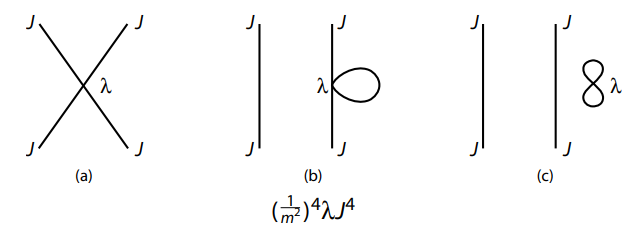
\includegraphics[scale=0.7]{feynman-diagram-1}
	\caption{From Zee}
\end{figure}\qed


\textit{Diagrams for $\sim (-\lambda)^2 J^4 / (m^2)^6$:} We expect to get 2 vertices, 4 external ends, and 6 lines. The following diagrams satisfy these conditions:\\

\begin{figure}[!htb]
	\centering
	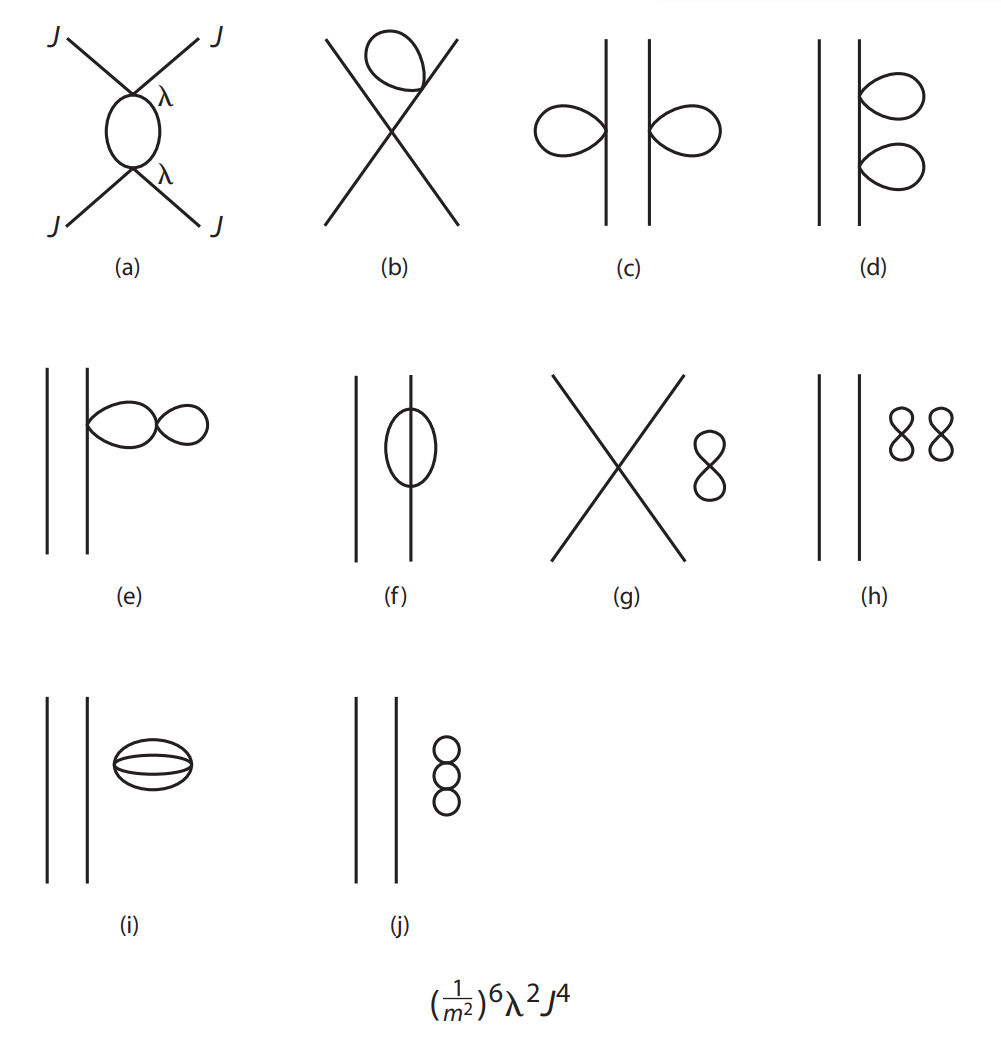
\includegraphics[scale=0.3]{feynman-diagram-2}
	\caption{From Zee}
\end{figure} \qed


\textit{Diagrams for $\sim (-\lambda)^2 J^6 / (m^2)^7$:} We expect to get 2 vertices, 6 external ends, and 7 lines. The following diagrams satisfy these conditions:\\

\begin{figure}[!htb]
	\centering
	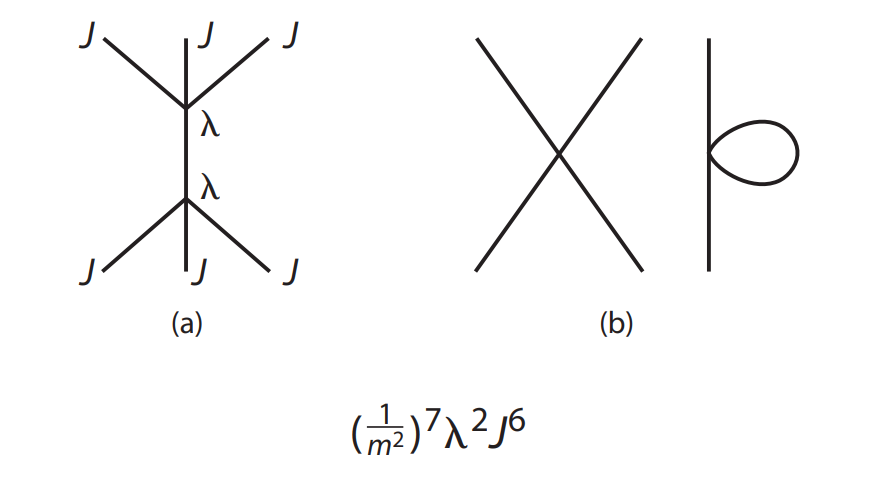
\includegraphics[scale=0.4]{feynman-diagram-3}
	\caption{From Zee}
\end{figure} \qed

Of course, we have seen that if we want a term with $\lambda^l$ and $J^j$ (where $j$ is even), i.e., $l$ vertices and $j$ external ends, then we have $(4l + j)$ lines.







\subsubsection{Another approach: Wick contraction}

Recall that in the baby problem we evaluated this integral
\begin{align}
\Z(J) = \int^\infty_{-\infty} dq\, \exp\lp -\f{1}{2}m^2 q^2 - \f{\lambda}{4!}q^4 + Jq \rp
\end{align}
by doing a power expansion in the $e^{\sim \lambda}$ term:
\begin{align}
\exp\lp -\f{1}{2!}\f{\lambda}{4!}q^4 \rp = 1 - \lp\f{\lambda}{4!}\rp q^4 + \f{1}{2!}\lp\f{\lambda}{4!}\rp^2 q^8 - \dots
\end{align}


If please, we can also re-do this problem starting out with a power expansion in $J$:
\begin{align}
\exp\lp Jq \rp = \sum^\infty_{s=0} \f{J^s q^s}{s!}.
\end{align}
With this, we can write and define the $G^{(s)}$ coefficients as
\begin{align}
\boxed{\Z(J) = \sum^\infty_{s=0} \f{J^s}{s!}\int_\mathbb{R}dq\, q^s \exp\lp -\f{1}{2}m^2 q^2 - \f{\lambda}{4!}q^4 \rp \equiv \Z(0,0) \sum^\infty_{s=0} \f{J^s}{s!} G^{(s)} }
\end{align}
These $G^{(6)}$ coefficients are analogues of Green's functions in field theory. \\

To evaluate the integral from here, we sort of repeat what we did earlier, except now we expand and differentiate under the integral sign with respect to $\lambda$. The coefficients $G^{(s)}$ can then be evaluated by the Wick contraction. We won't go into much detail about this for now. 












\subsubsection{Connected vs. Disconnected}

Looking at a few Feynman diagrams generated by our baby problem, we can see that some of them are connected while some aren't. For example, diagram $(a)$ for the $(1/m^2)^4\lambda J^4$ is connected, while $(b)$ and $(c)$ aren't. \\


Recall our definition of the generating function
\begin{align}
\Z(J, \lambda) = \Z(J=0, \lambda)e^{W(J,\lambda)} = \Z(J=0, \lambda)\sum^\infty_{N=0}\f{[W(J,\lambda)]^N}{N!}.
\end{align}



By definition the term $\Z(J=0, \lambda)$ consists of diagrams with no external source $J$. These diagrams look like loops such as Figure \ref{fig:loops}.

\begin{figure}[!htb]
	\centering
	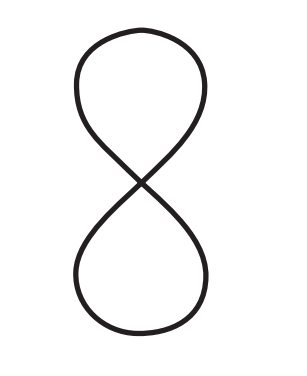
\includegraphics[scale=0.5]{feynman-diagram-4}
	\caption{From Zee}
	\label{fig:loops}
\end{figure}

So we see that while $W(J)$ is a sum of only connected diagrams, $\Z$ contains both types of diagrams, connected and disconnected. This is why $\Z$ is called the generating function, and $W$ is called the generating function for connected diagrams. 













\subsubsection{A child problem: Integrals, Wick contraction \& Propagation}


Before graduating to full field theory, let us try a slightly more difficult problem where we want to evaluate the following multiple integral
\begin{align}
\boxed{\Z(J) = \int_{\mathbb{R}^N} \prod_i^N dq_i \exp\lp -\f{1}{2}q^\top A q - \f{\lambda}{4!}q^4 + J\cdot q  \rp}
\end{align}
where
\begin{align}
q^4 = \sum_i q_i^4.
\end{align}
Notice that this an $N-$dimensional problem, and so $q$ are now vectors in some $N-$dimensional space, and $A$ is some matrix. We will assume that $A$ plays the role of some kind metric, which means it is positive definite and symmetric. In statistics, $A$ is the covariance matrix. In physics, $A$ can carry information about \textit{the} metric. \\

Recall our previous result:
\begin{align}
\Z(J)  = \sqrt{\f{2\pi}{m^2}} e^{-\f{\lambda}{4!}\lp \f{d}{dJ} \rp^4} e^\f{J^2}{2m^2}
\end{align}
starting from 
\begin{align}
\Z(J) = \int^\infty_{-\infty} dq\, \exp\lp -\f{1}{2}m^2 q^2 - \f{\lambda}{4!}q^4 + Jq \rp.
\end{align}


How do we generalize our result from the baby problem to this one in higher dimensions? To do this, we must first try an easier $n-$dimensional ``Gaussian integral'' such as
\begin{align}
I = \int \prod_i^N dx_i\, \exp\lp -\f{1}{2}x^\top A x \rp
\end{align}
where $A$ is again an positive definite and symmetric matrix (i.e., metric). We will first diagonalize $A$ with an orthogonal matrix $M$:
\begin{align}
D = MAM^{-1} = \text{diag}(\lambda_1, \lambda_2, \dots, \lambda_N)
\end{align}
where $\lambda_i$ are the eigenvalues of $A$. With this, 
\begin{align}
\det(A) = \det(D) = \prod_i^N \lambda_i
\end{align}The goal of doing this is so that we can ``de-couple'' the $x$'s in the exponent, by which we can bring the product sign outside of the integral. Once the product sign is outside of the integral, we will simply be left with a product of 1-dimensional Gaussian integrals. \\

We will also let
\begin{align}
z = M^\top x = (x^\top M)^\top.
\end{align}
The Jacobian of this change of basis is just the identity because $\det(M) = 1$, so we have
\begin{align}
I 
&= \int \prod_i^N dz_i\, \exp\lp -\f{1}{2}z^\top D z \rp \\ 
&= \prod_i^N \underbrace{\int dz_i\, \exp\lp -\f{1}{2}\lambda_i z_i^2\rp}_{\sqrt{2\pi / \lambda_i}} \hspace{0.5cm} D\text{ is diagonal}\\ 
&= \prod_i^N \sqrt{\f{2\pi}{  \lambda_i}}\\
&= \boxed{\sqrt{\f{(2\pi)^N}{\det(A)}}} \hspace{0.5cm}\text{since } \det(A) = \prod_i^N \lambda_i.
\end{align}

Nice! What if we added a source term? 
\begin{align}
I_J = \int \prod_i^N dx_i\, \exp\lp -\f{1}{2}x^\top A x + J^\top x \rp
\end{align}


Let $x = y + A^{-1}J$, then because $A = A^\top$, we must have that
\begin{align}
-\f{1}{2}x^\top A x + J^\top x &= -\f{1}{2}(y + A^{-1}J)^\top A (y + A^{-1}J) + J^\top (y + A^{-1}J)\nonumber\\
&= -\f{1}{2}\lb y^\top A y +2J^\top y + J^\top A^{-1}AA^{-1}J\rb + J^\top y + JA^{-1}J \nonumber\\
&= -\f{1}{2}y^\top A y + \f{1}{2}J^\top A^{-1}J.
\end{align}
Thus,
\begin{align}
I_J &= \int \prod_i^N dx_i\, \exp\lp -\f{1}{2}y^\top A y + \f{1}{2}J^\top A^{-1}J \rp\\
&= \exp\lp \f{1}{2}J^\top A^{-1}J \rp \int \prod_i^N dx_i\, \exp\lp -\f{1}{2}y^\top A y \rp \\
&= \boxed{ \sqrt{\f{(2\pi)^N}{\det(A)}} \exp\lp \f{1}{2}J^\top A^{-1}J \rp}
\end{align}

Let us now look back to the child problem. What we just did here with $n-$dimensional Gaussian integrals suggests expanding in $\lambda$ inside the integral first:
\begin{align}
\Z(J) &= \int_{\mathbb{R}^N} \prod_i^N dq_i  \exp\lp -\f{1}{2}q^\top A q - \f{\lambda}{4!}q^4 + J^\top q  \rp \nonumber \\ 
&= \int_{\mathbb{R}^N} \prod_i^N dq_i  \exp\lp -\f{1}{2}q^\top A q + J^\top q \rp
\lc \sum_{j=0}^\infty   \f{\lb -\f{\lambda}{4!}q^4\rb^j}{j!}  \rc \nonumber \\
&= \int_{\mathbb{R}^N} \prod_i^N dq_i  \exp\lp -\f{1}{2}q^\top A q + J^\top q \rp
\lc 1 -\f{\lambda}{4!}q^4 + \f{1}{2!}\lp-\f{\lambda}{4!}q^4\rp^2 + \dots   \rc  
\end{align}

To evaluate this integral, we integrate term-by-term, using the Feynman's differentiating under the integral sign. But we have first be very careful here because we're dealing with vectors. Recall that
\begin{align}
q^4 = \sum_i q_i^4.
\end{align}
Every factor of $\p / \p J_{i}$ brings down a factor of $q_i$. So, in order to get any $q^4$ term, we need
\begin{align}
\sum_i \lp\f{\p}{\p J_i}\rp^4.
\end{align}
Thus 
\begin{align}
\exp\lp \f{-\lambda q^4}{4!} \rp \sim \exp\lb \f{-\lambda }{4!} \lp\sum_i \f{\p }{\p J_i} \rp^4\rb.
\end{align}
Therefore, from integrating term-by-term by differentiating under the integral sign, then adding the terms up together we get that
\begin{align}
\Z(J) &= \lc 1 + \lb\f{-\lambda}{4!} \lp\sum_i \f{\p }{\p J_i} \rp^4\rb + \f{1}{2!}\lb\f{-\lambda }{4!} \lp\sum_i \f{\p }{\p J_i} \rp^4\rb^2 + \dots   \rc \nonumber \\
&\,\,\,\,\,\hspace{1cm}\times\int_{\mathbb{R}^N} \prod_i^N dq_i  \exp\lp -\f{1}{2}q^\top A q + J^\top q \rp \nonumber\\
&= \exp\lb \f{-\lambda q^4}{4!} \lp\sum_i \f{\p }{\p J_i} \rp^4\rb \times \lb  \int_{\mathbb{R}^N} \prod_i^N dq_i  \exp\lp -\f{1}{2}q^\top A q + J^\top q \rp\rb \nonumber\\
&= \sqrt{\f{(2\pi)^N}{\det(A)}}\exp\lb \f{-\lambda q^4}{4!} \lp\sum_i \f{\p }{\p J_i} \rp^4\rb  \exp\lb \f{1}{2}J^\top A^{-1}J \rb,
\end{align}
where we of course have just evaluated the last integral by a change of variables. With this result, we can write more compactly
\begin{align}
\boxed{\Z(J) =  \sqrt{\f{(2\pi)^N}{\det(A)}}\, e^{-(\lambda/4!) \sum_i (\p/\p J_i)^4} \, e^{\f{1}{2}J^\top A^{-1} J}}
\end{align}




Alternatively, we can first expand in powers of $J$ first, before in powers of $\lambda$. Let's start with the expansion in $J$:
\begin{align}
\Z(J) &= \int_{\mathbb{R}^N} \prod_i^N dq_i  \exp\lp -\f{1}{2}q^\top A q - \f{\lambda}{4!}q^4 + J^\top q  \rp \nonumber \\ 
&= \int_{\mathbb{R}^N} \prod_i^N dq_i  \exp\lp -\f{1}{2}q^\top A q - \f{\lambda}{4!}q^4 \rp \lc \sum^\infty_{s=0} \f{(J^\top q)^s}{s!}  \rc \nonumber \\ 
&= \int_{\mathbb{R}^N} \prod_i^N dq_i  \exp\lp -\f{1}{2}q^\top A q - \f{\lambda}{4!}q^4 \rp \lc \sum^\infty_{s=0} \f{\lb \sum_{l_s}^N (J_{l_s} q_{l_s}) \rb^s}{s!}  \rc \nonumber \\ 
&= \sum^\infty_{s=0} \sum^N_{l_1 = 1}\dots \sum^N_{l_s = 1} \f{1}{s!}J_{l_1}\dots J_{l_s} \int_{\mathbb{R}^N} \lp\prod_i^N dq_i \rp \exp\lp -\f{1}{2}q^\top A q - \f{\lambda}{4!}q^4 \rp q_{l_1}\dots q_{l_s}\nonumber\\
&\equiv \boxed{\Z(0,0) \sum^\infty_{s=0} \sum^N_{l_1 = 1}\dots \sum^N_{l_s = 1} \f{1}{s!}J_{l_1}\dots J_{l_s} G^{(s)}_{l_1 \dots l_s}}
\end{align}
where we defined the Green's function coefficients such that
\begin{align}
\boxed{\Z(0,0) G^{(s)}_{l_1 \dots l_s} \equiv \int_{\mathbb{R}^N} \lp\prod_i^N dq_i \rp \exp\lp -\f{1}{2}q^\top A q - \f{\lambda}{4!}q^4 \rp q_{l_1}\dots q_{l_s}}
\end{align}


One main difference between the child problem and the baby problem is that the Green's function coefficients in the child problem have indices. What this means is that we have \textit{propagation from here to there}. Also, notice that these coefficients with an \textbf{odd} number of indices are \textbf{zero}, since the integrand in these cases are odd functions. \\

To see what these $G$ coefficients are we should try to evaluate a few illuminating examples. Let us start with the ``2-point Green's function'' to zeroth order in $\lambda$. The strategy to evaluate this integral is to put back a $J$ into the exponent and differentiate in order to get the $q$ terms in the integrand, then set $J=0$. We note that every factor of $\p / \p J_{l_s}$ gives a factor of $q_{l_s}$. Let's proceed:
\begin{align}
G^{(2)}_{l_1l_2}(\lambda = 0) &= \f{1}{\Z(0,0)}\int_{\mathbb{R}^N} \lp\prod_i^N dq_i \rp \exp\lp -\f{1}{2}q^\top A q  \rp q_{l_1}q_{l_2} \nonumber \\ 
&= \f{1}{\Z(0,0)}\int_{\mathbb{R}^N} \lp\prod_i^N dq_i \rp \exp\lp -\f{1}{2}q^\top A q  + J^\top q  \rp q_{l_1}q_{l_2}\bigg\vert_{J=0}\nonumber\\
&= \f{1}{\Z(0,0)}\int_{\mathbb{R}^N} \lp\prod_i^N dq_i \rp \f{\p}{\p J_{l_1}} \f{\p}{\p J_{l_2}} \exp\lp -\f{1}{2}q^\top A q  + J^\top q  \rp \bigg\vert_{J=0}\nonumber\\
&= \underbrace{\f{1}{\Z(0,0)}}\f{\p}{\p J_{l_1}} \f{\p}{\p J_{l_2}} \underbrace{ \int_{\mathbb{R}^N} \lp\prod_i^N dq_i \rp  \exp\lp -\f{1}{2}q^\top A q  + J^\top q  \rp} \bigg\vert_{J=0}\nonumber\\
&= \lp \sqrt{\f{(2\pi)^N}{\det(A)}}\rp^{-1}\f{\p}{\p J_{l_1}} \f{\p}{\p J_{l_2}} \lp\sqrt{\f{(2\pi)^N}{\det(A)}}\rp\exp\lp \f{1}{2} J^\top A^{-1}J \rp \bigg\vert_{J=0} \nonumber\\
&= \f{\p}{\p J_{l_1}} \f{\p}{\p J_{l_2}} \exp\lp \f{1}{2} J^\top A^{-1}J \rp \bigg\vert_{J=0}\nonumber\\
&= \lc\f{\p}{\p J_{l_1}} \f{\p}{\p J_{l_2}}\lp \f{1}{2}J^\top A^{-1}J \rp \rc \exp\lp \f{1}{2} J^\top A^{-1}J \rp \bigg\vert_{J=0}\nonumber\\
&= \f{\p}{\p J_{l_1}} \f{\p}{\p J_{l_2}} \lp \f{1}{2}J^\top A^{-1}J\rp \nonumber\\
&= \f{1}{2}\lp A^{-1}_{l_1l_2} + A^{-1}_{l_1l_2} \rp \nonumber\\
&= \boxed{A^{-1}_{l_1l_2}}
\end{align}
where we have used the fact that $A^{-1}$ is symmetric. The last equality follows from the fact that because we have $J$ and $J^\top$ and the derivatives $\p / \p_{l_1}$ and $\p / \p_{l_2}$, which together annihilate all other matrix elements of $A^{-1}$ except $A^{-1}_{l_1l_2}$ and $A^{-1}_{l_2l_1}$, which are equal because $A^{-1}$ is symmetric just as $A$. We thus have an important result:
\begin{align}
\boxed{G^{(2)}_{ij}(\lambda = 0) = A^{-1}_{ij} = A^{-1}_{ji}}
\end{align}

The matrix element $A^{-1}_{ij}$ describes propagation from $i \to j$. \qed\\


What about a ``4-point Green's function'' to order $\lambda$?
\begin{align}
G^{(4)}_{l_1l_2l_3l_4} &= \f{1}{\Z(0,0)} \int_{\mathbb{R}^N} \lp\prod_i^N dq_i \rp \exp\lp -\f{1}{2}q^\top A q  \rp q_{l_1}q_{l_2}q_{l_3}q_{l_4} \lb 1 - \f{\lambda}{4!}q^4 + o(\lambda^2) \rb \nonumber \\
&= \f{1}{\Z(0,0)} \int_{\mathbb{R}^N} \lp\prod_i^N dq_i \rp e^{ -\f{1}{2}q^\top A q  } q_{l_1}q_{l_2}q_{l_3}q_{l_4} \lb 1 - \f{\lambda}{4!} \sum_n q_n^4 + o(\lambda^2) \rb.
\end{align}

Here, we note that because $A^{-1}$ is a matrix, it can only carry two indices at a time. So, to evaluate the first part of this integral (the part multiplied by $\lambda^0$), we do it with two $q$ terms at a time. By inspection, we get a product of two matrix elements of $A^{-1}$. There are six ways to pick 2 things out of 4, but because $A^{-1}$ symmetric, we are left with three terms. The factor of $1/2$ from the exponent comes down to annihilate the factors of $2$ in each of the three terms. 
\begin{align}
\f{1}{\Z(0,0)} \int_{\mathbb{R}^N} \lp\prod_i^N dq_i \rp e^{ -\f{1}{2}q^\top A q  } q_{l_1}q_{l_2}q_{l_3}q_{l_4} = A^{-1}_{l_1l_2}A^{-1}_{l_3l_4} + A^{-1}_{l_1l_3}A^{-1}_{l_2l_4} + A^{-1}_{l_1l_4}A^{-1}_{l_3l_2}.
\end{align}
What about the $\lambda/4!$ integral? Well first notice that it by itself is a sum. So it suffices just to evaluate it for $n=k$. Consider:
\begin{align}
&\,\,\f{1}{\Z(0,0)} \int_{\mathbb{R}^N} \lp\prod_i^N dq_i \rp e^{ -\f{1}{2}q^\top A q  } q_{l_1}q_{l_2}q_{l_3}q_{l_4} \lb  - \f{\lambda}{4!} q_k^4  \rb \\ 
= &\,\, \f{1}{\Z(0,0)} \lp \f{-\lambda}{4!} \rp \int_{\mathbb{R}^N} \lp\prod_i^N dq_i \rp e^{ -\f{1}{2}q^\top A q  } q_{l_1}q_{l_2}q_{l_3}q_{l_4}q_k q_k q_k q_k. 
\end{align}


Now, we observe that $q_{l_1}$ has four choices of $q_k$'s to contract with, $q_{l_2}$ has three choices of $q_k$'s to contract with, and so on, producing a factor of $4!$. This is exactly why we originally define the $\lambda$ term along with the factor of $1/4!$. They conveniently cancel and leave us with
\begin{align}\label{high-moment}
 &\,\, \f{1}{\Z(0,0)} \lp \f{-\lambda}{4!} \rp \int_{\mathbb{R}^N} \lp\prod_i^N dq_i \rp e^{ -\f{1}{2}q^\top A q  } q_{l_1}q_{l_2}q_{l_3}q_{l_4}\sum_{n}q_n^4 \nonumber \\
=&\,\,  -\lambda  \sum_n A^{-1}_{l_1n}A^{-1}_{l_2n}A^{-1}_{l_3n}A^{-1}_{l_4n} + \dots
\end{align}
where the overall constants are all canceled out in the end. We are also leaving out the contractions of $q_n$'s with themselves. This is because these self-contractions give us the first three terms (involving $l_1, l_2, l_3, l_4$) multiplied by $A^{-1}_{nn}A^{-1}_{nn}$. We will simply deal with this later. \\

With that said, the 4-point Green's function is
\begin{align}
G^{(4)}_{l_1l_2l_3l_4} &= A^{-1}_{l_1l_2}A^{-1}_{l_3l_4} + A^{-1}_{l_1l_3}A^{-1}_{l_2l_4} + A^{-1}_{l_1l_4}A^{-1}_{l_3l_2} \nonumber\\
&\hspace{1.5cm}-\lambda \sum_n A^{-1}_{l_1n}A^{-1}_{l_2n}A^{-1}_{l_3n}A^{-1}_{l_4n} + \dots + O(\lambda^2)
\end{align}

The first three terms describe one excitation propagating from $l_1$ to $l_2$ and another propagation from $l_3$ to $l_4$, plus the two possible permutations on this history. The order $\lambda$ term tells us that four excitations, propagating from $l_1$ to $n$, $l_2$ to $n$, $l_3$ to $n$, nd $l_4$ to $n$, meet at $n$ and interact with an amplitude proportional to $\lambda$, where $n$ anywhere on the lattice. 


























\subsubsection{Perturbative field theory}



Now that we're done with the baby and child problems, let us turn to the integral we've been wanting to evaluate:
\begin{align}
\boxed{\Z(J) = \int \mathfrak{D}[\phi] \exp\lp i\int d^4x\,  \f{1}{2}\lb(\p \phi)^2 - m^2 \phi^2 \rb - \f{\lambda}{4!}\phi^4 + J(x)\phi \rp}
\end{align}

There are a few key differences between this integral and the ones in the baby and child problems. First, there is a factor of $i$ in the exponent. Second, we no longer have a single variable $y$ or a single vector $q$ but instead have $\phi(x)$, which is a function of a continuous four-vector $x$. Third, the source $J$ is also a function of a continuous variable $x$. This is very different from what we had before where we were dealing with points on a lattice and things are discrete. \\

However, it turns out that the structure of things are quite the same. Remember that in the child problem if we first expand in $\lambda$, followed by in $J$, then we have
\begin{align}
\Z(J) =  \sqrt{\f{(2\pi)^N}{\det(A)}}\, e^{-(\lambda/4!) \sum_i (\p/\p J_i)^4} \, e^{\f{1}{2}J^\top A^{-1} J}.
\end{align}
In our new problem, things are continuous, so we simply replace sums by Riemann integrals.\\

If we again \textit{start by expanding in the $\lambda$ term}, then
\begin{align}
\Z(J)= \exp\lb \f{-i\lambda}{4!} \int d^4w\lp \f{\delta}{i \delta  J(w)}\rp^4 \rb \int \mathfrak{D}\phi e^{ i\int d^4x\,  \f{1}{2}\lb(\p \phi)^2 - m^2 \phi^2 \rb + J(x)\phi }.
\end{align} 

Now, recall that with
\begin{align}
\tilde{\Z}_J = \int \mathfrak{D}[\phi]\, \exp\lc i\int d^4x\, \lb \f{1}{2}\p_\mu \phi \p^\mu \phi - \f{1}{2}m^2\phi^2 + J(x)\phi(x) \rb \rc,
\end{align}
integrating by parts in the integrand in the exponent:
\begin{align}
\int d^4x\,\p_\mu \lb \phi \p^\mu \phi \rb &= \int d^4x\, \p_\mu \phi \p^\mu \phi   + \int d^4x\, \phi \square \phi \\ 
\phi\p^\mu\phi\bigg\vert^\infty_{-\infty} &= \int d^4x\, \p_\mu \phi \p^\mu \phi   + \int d^4x\, \phi \square \phi  \\ 
0 &= \int d^4x\, \p_\mu \phi \p^\mu \phi   + \int d^4x\, \phi \square \phi
\end{align}
which gives
\begin{align}
\Z = \int \mathfrak{D}[\phi]\, \exp\lc i\int d^4x\, \lb -\f{1}{2}\phi(\square + m^2) \phi  + J(x)\phi(x) \rb\rc.
\end{align}


Also, remember that earlier in this section we called
\begin{align}
A = -(\square + m^2)
\end{align}
and defined the propagator $\D$ as the inverse of $A$ such that
\begin{align}
-(\square + m^2)\D(x-y) = \delta^4(x-y).
\end{align}
Therefore, we must have that
\begin{align}
\tilde{\Z}_J &= \int \mathfrak{D}[\phi]\exp\lc i\int d^4x \,\lb \f{1}{2} \phi A \phi + J(x)\phi \rb\rc \nonumber\\
&= \exp\lc \f{-i}{2}JA^{-1}J \rc \hspace{0.5cm}\text{Gaussian integral, remember?} \nonumber \\ 
&= \exp\lc -\f{i}{2}\iint d^4x d^4y\, J(x)\D(x-y)J(y) \rc \hspace{0.5cm}\text{by definition.}
\end{align}
With this, we have
\begin{align}
\boxed{\Z(J) = \Z(0,0)e^{ -i\lambda/4! \int d^4w\, [\delta/i \delta  J(w)]^4 } e^{ (-i/2)\iint d^4x d^4y\, J(x)\D(x-y)J(y) }}
\end{align}

And thus the structure of the answer is exactly the same as before. \\

Next, let us look at how the form of the propagator has changed. The the baby problem, the propagator is essentially $1/M^2$. In the child problem, the propagator is given by $A^{-1}$. Here, however, the propagator in momentum space is given by
\begin{align}
\boxed{\D(x-y) = \int \f{d^4k}{(2\pi)^4} \f{e^{ik\cdot(\vec{x} - \vec{y})}}{k^2 - m^2 + i\epsilon}}
\end{align}
which we should quite familiar with at this point. To remember how this propagator is constructed, simply think of $\D(x-y)$ as the inverse of $-(\square+m^2)$. Write down the equation that says this that involves the delta function, then look at the Fourier transform of both sides. Then, use the relationship between $\D(x-y)$ and its transform $\D(k)$ to work out what $\D(x-y)$ ought to be. Please refer to the beginning of this section for details. \\


We also know that $J(x)$ corresponds to sources and sinks. So, if we expand $\Z(J)$ as a series of $J$ first, the powers of $J$ would indicate the number of particles involved in the process. This is why in particle physics it makes sense to specify the power of $J$. So, let us start evaluating the integral by an expansion first in $J$. From 
\begin{align}
\Z(J) = \int \mathfrak{D}[\phi] \exp\lp i\int d^4x\,  \f{1}{2}\lb(\p \phi)^2 - m^2 \phi^2 \rb - \f{\lambda}{4!}\phi^4 + J(x)\phi \rp
\end{align}
we get from expanding in $J$:
\begin{align}
\Z(J) &=  \int \mathfrak{D}[\phi] \exp\lp i\int d^4x\,  \f{1}{2}\lb(\p \phi)^2 - m^2 \phi^2 \rb - \f{\lambda}{4!}\phi^4\rp \exp\lp i\int d^4x\, J(x)\phi \rp \nonumber \\ 
&= \int \mathfrak{D}[\phi] \exp\lp i\int d^4x\,  \f{1}{2}\lb(\p \phi)^2 - m^2 \phi^2 \rb - \f{\lambda}{4!}\phi^4\rp \lc \sum_{s=0}^\infty \f{\lb  i\int d^4x\, J(x)\phi \rb^s}{s!} \rc \nonumber\\
&= \sum^\infty_{s=0}\f{i^s}{s!}\int dx_1\dots dx_s J(x_1)\dots J(x_s)\times\nonumber\\
 &\hspace{1cm}\times \int \mathfrak{D}[\phi] \exp\lp i\int d^4x\,  \f{1}{2}\lb(\p \phi)^2 - m^2 \phi^2 \rb - \f{\lambda}{4!}\phi^4\rp \phi(x_1)\dots \phi(x_s) \nonumber\\
&=  \sum^\infty_{s=0}\f{i^s}{s!}\int dx_1\dots dx_s J(x_1)\dots J(x_s) \lb \Z(0,0)G^{(s)}(x_1,\dots,x_s) \rb \nonumber\\
&= \boxed{\Z(0,0)	\sum^\infty_{s=0}\f{i^s}{s!}\int dx_1\dots dx_s J(x_1)\dots J(x_s)  G^{(s)}(x_1,\dots,x_s) } \nonumber
\end{align}
where we define 
\begin{align}
\boxed{\Z(0,0)\,G^{(s)}(x_1,\dots,x_s) = \int \mathfrak{D}[\phi] e^{ i\int d^4x\, \lb \f{1}{2}(\p \phi)^2 - m^2 \phi^2 \rb - \f{\lambda}{4!}\phi^4} \phi(x_1)\dots \phi(x_s)}
\end{align}
and of course
\begin{align}
\boxed{\Z(0,0) \equiv  \int \mathfrak{D}[\phi] e^{ i\int d^4x\,  \f{1}{2}\lb(\p \phi)^2 - m^2 \phi^2 \rb}}
\end{align}



Just as before, let us look at the 2-point Green's function:
\begin{align}\label{g2}
G^{(2)}(x_1,x_2) \equiv \f{1}{\Z(0,0)} \int \mathfrak{D}[\phi] e^{ i\int d^4x\,  \f{1}{2}\lb(\p \phi)^2 - m^2 \phi^2 \rb - \f{\lambda}{4!}\phi^4} \phi(x_1)\phi(x_2).
\end{align}
And the 4-point Green's function is 
\begin{align}
G^{(4)}(x_1,x_2,x_3,x_4) \equiv \f{1}{\Z(0,0)} \int \mathfrak{D}[\phi] e^{ i\int d^4x\,  \f{1}{2}\lb(\p \phi)^2 - m^2 \phi^2 \rb - \f{\lambda}{4!}\phi^4} \phi(x_1)\phi(x_2)\phi(x_3)\phi(x_4).
\end{align}
We can generate more at will, of course (hence why $\Z(J)$ is called the generating function). Because the propagators are translation invariant, $G^{(2)}(x_1,x_2)$ only depends on $x_1 - x_2$, but not explicitly $x_1$ and $x_2$. Similarly, the 4-point Green's function only depends on the spacings between the $x_i$'s. For $\lambda = 0$, we see that the 2-point Green's function reduces to $i\D(x_1 - x_2)$. We can show this first generally by recalling that
\begin{align}
\Z(J) \equiv \Z(0,0)\Z(0,0)\exp\lc -\f{i}{2}\iint d^4x_1d^4x_2\, J(x_1)\D(x_1-x_2) J(x_2) \rc
\end{align}
which comes from the very beginning when we defined generating function and propagators in terms of the transforms, etc. What we will do now is do a power series expansion:
\begin{align}
\f{\Z(J)}{\Z(0,0)} = \sum^\infty_{s=0}&\f{1}{s!}\lp\f{-i}{2}\rp^2 \int d^4x_1\dots d^4_{x_{2s}}J(x_1)\dots J(x_{2s})\nonumber\\
&\hspace{2cm}\times \D(x_1 - x_2)\dots \D(x_{2n-1} - x_{2x})
\end{align}
where only even powers of $J$ can appear. Now, compare this to the equation we have just gotten:
\begin{align}
\f{\Z(J)}{\Z(0,0)} = 	\sum^\infty_{s=0}\f{i^s}{s!}\int dx_1\dots dx_s J(x_1)\dots J(x_s)  G^{(s)}(x_1,\dots,x_s).
\end{align}
By reading off the correct terms, we have roughly that
\begin{align}
\f{i^{2n}}{(2n)!}G^{(2n)}(x_1,\dots,x_{2n}) \sim \f{1}{n!}\lp \f{-i}{2} \rp^n \lb \D(x_1-x_2)  \dots \D(x_{2n-1} - x_{2n})\rb
\end{align}
where $\sim$ simply denotes that we're close up to symmetrization. However, for $s = 2 \iff n = 1$, we have exactly that
\begin{align}
\f{-1}{2!}G^{(2)}(x_1, x_2) = \f{1}{1!}\lp \f{-i}{2} \rp \D(x_1 - x_2).
\end{align}
This means 
\begin{align}
\boxed{G^{(2)}(x_1,x_2) = i\D(x_1 , x_2)}
\end{align}
as desired.  \qed\\

The relationship between the Green's function and the propagators $\D$ will be explored in the following subsections as we better understand Feynman rules and Feynman diagrams.\\

We observe that while $\D(x_1 - x_2)$ describes the propagation of a particle between $x_1$ and $x_2$ in the \textbf{absence} of interaction (we have pointed out this fact before), $G^{(2)}(x_1,x_2)$, which is called the \textit{correlation function}, describes the propagation of a particle between $x_1$ and $x_2$ with \textbf{interaction}. This nomenclature possibly comes from the resemblance between $G^{(s)}$ and higher moments of the Gaussian, which are called \textit{correlation functions}. This resemblance is reflected in Eq \eqref{g2}. We see that this integral looks like a second moment of the Gaussian.\\

To summarize, we said that $G^{(2)}$ is a correlation function describing a propagation with interaction. In general, $G^{(4)}_{ijkl}$, say, describes the scattering of particles. \\


In some sense, it seems that we can do QFT in two ways:
\begin{enumerate}
	\item \textbf{Schwinger:} Starting with expansion in $\lambda$, then expand in $J$.
	\item \textbf{Wick:} Starting with expansion in $J$, then expand in $\lambda$.
\end{enumerate}

But \textbf{Feynman} diagrams capture both approaches by representing terms in the final double expansion. 

















\subsubsection{Collision between particles}



In this section, we will set up two sources and two sinks to watch two particles (mesons) scatter off each other. Here's the setup:
\begin{figure}[!htb]
	\centering
	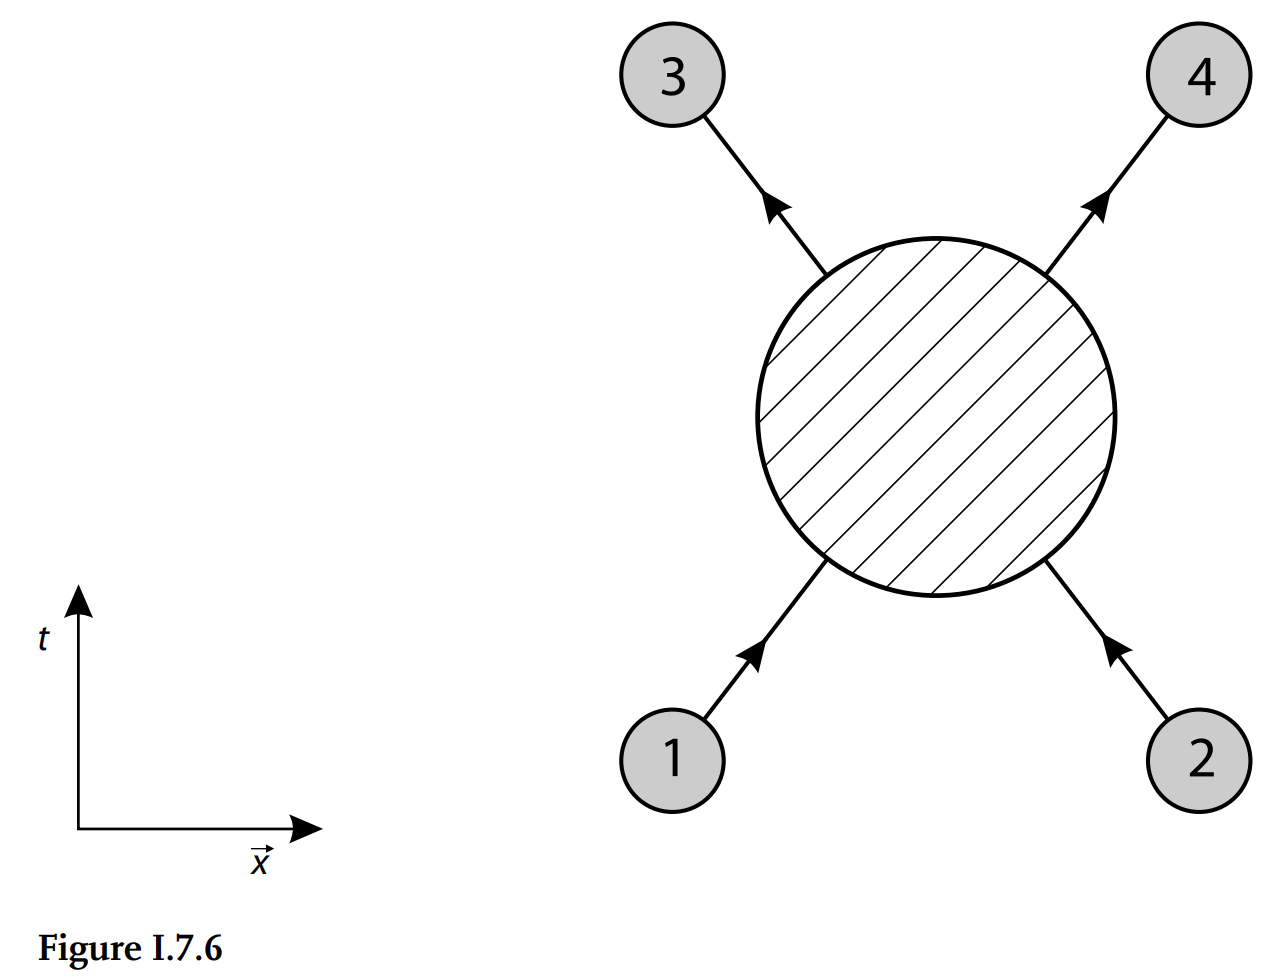
\includegraphics[scale=0.3]{mesons}
	\caption{From Zee}
\end{figure}\\

It suffices to find in $\Z$ a term containing $J(x_1)J(x_2)J(x_3)J(x_4)$. But we notice that this is just $G^{(4)}(x_1,x_2,x_3,x_4)$.\\

Let's start from the Wick way first. Recall that $G^{(4)}$ is given by
\begin{align}
G^{(4)}(x_1,x_2,x_3,x_4) = \f{1}{\Z(0,0)}\int \mathfrak{D}[\phi]e^{i\int d^4x\, \f{1}{2}[(\p \phi)^2 - m^2\phi^2]- \f{\lambda}{4!}\phi^4}\phi(x_1)\phi(x_2)\phi(x_3)\phi(x_4).
\end{align}
Expanding in $\lambda$ gives
\begin{align}
G^{(4)}(x_1,x_2,x_3,x_4) = \f{1}{\Z(0,0)}&\int \mathfrak{D}[\phi]e^{i\int d^4x\, \f{1}{2}[(\p \phi)^2 - m^2\phi^2]}\nonumber\\
&\times  \phi(x_1)\phi(x_2)\phi(x_3)\phi(x_4) \sum^\infty_{s=0}\f{\lp - \f{i\lambda}{4!}\int d^4w\,\phi^4(w)\rp^s}{s!}.
\end{align}
To first order, i.e., $s=1$, we have
\begin{align}
G^{(4)}(x_1,x_2,x_3,x_4) = \f{1}{\Z(0,0)}&\lp \f{-i\lambda}{4!} \rp\int d^4w\int \mathfrak{D}[\phi]e^{i\int d^4x\,\f{1}{2}[(\p \phi)^2 - m^2\phi^2]}\nonumber\\ &\times\phi(x_1)\phi(x_2)\phi(x_3)\phi(x_4)\phi^4(w).
\end{align}
By staring at this integral for a bit we recognize that it is a more complicated case of the high-moment Gaussian integral we have encountered before in Eq \eqref{high-moment}, where the sum in simply replaced by an integral, and the overall integral is multiplied by a factor of $i$. Once again, $\phi(x_1)$ has four choices of $\phi(w)$ to contract with, and so on, so that in the end the factor of $4!$ is canceled. Once the Feynman's trick to differentiate under the integral sign is done correctly, we will get
\begin{align}\label{four-sources}
\boxed{G^{(4)}(x_1,x_2,x_3,x_4) = \f{-i\lambda}{\Z(0,0)}\int d^4w\, \D(x_1 - w)\D(x_2 - w)\D(x_3 - w)\D(x_4 - w)}
\end{align}
which not surprisingly completely shares the structure of Eq \eqref{high-moment}. Now, compare this to what we found when we tried to show $G^{(2)} = i\D$, we see that we wouldn't be quite right to just set $G = $ products of $\D$. What we see here is that $G$ is a summation over all possible products of $\D_{iw}$ over all $w$. This is the accurate relationship between the Green's functions and the propagators. It follows from this that $G^{(2)}_{ab} = i\D_{ab}$.  \\

What about the Schwinger way where we first expand in $J$? Well, we start out with
\begin{align}
\Z(J) = \Z(0,0)e^{ -i\lambda/4! \int d^4w\, [\delta/i \delta  J(w)]^4 } e^{ (-i/2)\iint d^4x d^4y\, J(x)\D(x-y)J(y) }
\end{align}
and replace the first exponential with only first order terms in $J$. Once this is done, we get
\begin{align}
\Z(J) = \Z(0,0)\lb -\lp\f{i\lambda}{4!}\rp \int d^4w \lp \f{\delta}{\delta J(w)} \rp^4 \rb e^{ (-i/2)\iint d^4x d^4y\, J(x)\D(x-y)J(y) }.
\end{align}
Next, we expand the exponential and find the term with the fourth order of $\D$ (since we're looking for a term describing four propagations)
\begin{align}
e^{ (-i/2)\iint d^4x d^4y\, J(x)\D(x-y)J(y) } = \sum^\infty_{s=0}\f{[(-i/2)\iint d^4x d^4y\, J(x)\D(x-y)J(y)]^s}{s!}.
\end{align}
The fourth order term is 
\begin{align}
\f{1}{4!}\lp \f{-i}{2} \rp^4\lb \iint d^4x d^4y\, J(x)\D(x-y)J(y)  \rb^4.
\end{align}
Thus the term in first order $\lambda$ and fourth order $\D$ is
\begin{align}
\lb -\lp\f{i\lambda}{4!}\rp \int d^4w \lp \f{\delta}{\delta J(w)} \rp^4 \rb\lp\f{1}{4!}\rp\lp \f{-i}{2} \rp^4\lb \iint d^4x d^4y\, J(x)\D(x-y)J(y)  \rb^4.
\end{align}
After some cleaning up the algebra and renaming we get
\begin{align}\label{multi-J}
\boxed{\sim i\lambda \int_w \lp \f{\delta}{\delta J(w)} \rp^4 \bigintss^{(8)}  \D_{ae}\D_{bf}\D_{cg}\D_{dh}J_aJ_bJ_cJ_dJ_eJ_fJ_gJ_h}
\end{align}
where the very big integral denotes 8 integrals; $\D_{ij} \equiv \D(x_i - x_j)$; $J(x_a) = J_a$; $\int_a = \int d^4x_a$. \\

We notice that the four $[\delta/\delta J(w)]$'s will hit the $J$'s of course. The $\delta/\delta J(w)$ acts like a delta function:
\begin{align}
\f{\delta}{\delta J(w)}J_a = \delta(a-w).
\end{align}
So, for example.
\begin{align}
\f{\delta}{\delta J(w)}\int \D_{ae}J_e = \int \D_{ae}\delta (e-w)J_e = \D_{aw}.
\end{align}
We can write all this out, but in the end not all terms will be of interest of us. In particular, there will be three terms, two of which are disconnected (so the $\D_{ij}$'s don't share any common $x_i$). The only connected term is:
\begin{align}
\sim -i\lambda \int_w  \iiiint \D_{aw}\D_{bw}\D_{cw}\D_{dw}J_aJ_bJ_cJ_d
\end{align}
where we have reduced the number of integrals because of the delta function. \\

Okay. Why did we do all of this? The \textbf{goal} here is to see two particles (mesons) created by some localized source, scatter off each other, and disappear into localized sinks. So, if we set the source and sinks to be delta functions:
\begin{align}
J_i = \delta(x - x_i), \hspace{1cm} x = 1,2,3,4
\end{align}
then we have
\begin{align}
&-i\lambda \int_w  \iiiint \D_{aw}\D_{bw}\D_{cw}\D_{dw}J_aJ_bJ_cJ_d \\
=\,\,&i\lambda \int_w  \iiiint \D_{aw}\D_{bw}\D_{cw}\D_{dw}\delta(1)\delta(2)\delta(3)\delta(4) \\ 
=\,&\boxed{-i\lambda \int_w \D_{1w}\D_{2w}\D_{3w}\D_{4w}}
\end{align}
This is exactly what we found in Eq \eqref{four-sources}, up to some constants we haven't accounted for of course. \\

What does it all mean? The result is this: 2 particles from $x_1$ and $x_2$ propagate to the spacetime point $w$ (\textit{every possible $w$}), with amplitude $\D(x_1 - w)\D(x_2 - w)$, scatter with amplitude $-i\lambda$, then propagate from $w$ to $x_3$ and $x_4$ with amplitude $\D(x_3 - w)\D(x_4 - w)$. The integration over all spacetime $\int_w \equiv \int d^4w$ just means that the propagation to $w$ could have been anywhere. This comes back to the child problem!
\begin{figure}[!htb]
	\centering
	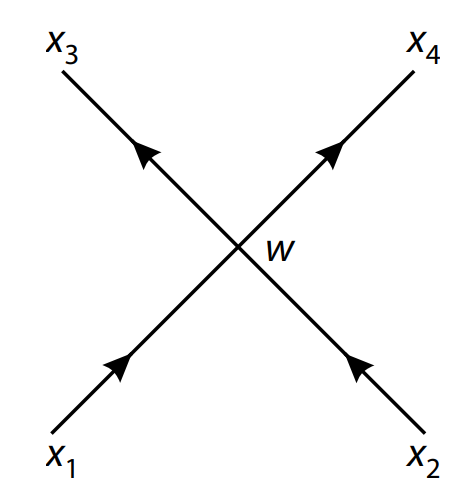
\includegraphics[scale=0.3]{propagates}
	\caption{From Zee}
\end{figure}















\subsubsection{Feynman diagrams: The rules}

So what are the rules for Feynman diagrams? Do we have to do all this integration and expansion every time to calculate the Green's function/correlation function? I think it's clear at this point a lot we have done so far has been by analogy: we begin to form associations between objects such as $q \to \phi$, sum $\to$ integral, and so on. What are the underlying rules here? What is the relationship between Feynman diagrams in position (spacetime) space and momentum space? \\

Sometimes it is easier for us to go pass to momentum space. Hypothetically, a particle with momentum $k_1$ and a particle with momentum $k_2$ collide and scatter, emerging with momentum $k_3$ and $k_4$. Each spacetime propagator has the form
\begin{align}
\D(x_a - w) = \F[\D(k_a)](x_a) = \int \f{d^4k_a}{(2\pi)^4} \f{e^{\pm ik_a(x_a - w)}}{k_a^2 - m^2 + i\epsilon}
\end{align}
where $\F$ denotes the Fourier transform of course and the sign assignment to $k_a$ can be made arbitrary because the ``volume'' element always corrects for that. Thus the overall $G^{(4)}$ (or the correlation function) up to leading constants has the form:
\begin{align}
-i\lambda \int_w \D_{1w}\D_{2w}\D_{3w}\D_{4w} &\sim \int d^4w \, \exp\lp -i(k_1 + k_2 - k_3 - k_4) \rp \\
&= (2\pi)^4\delta^{(4)}(k_1 + k_2 - k_3 - k_4).
\end{align}
So, the fact that the interaction can occur anywhere in spacetime translate to conservation of momentum:
\begin{align}
k_1 + k_2 = k_3 + k_4.
\end{align}
\begin{figure}[!htb]
	\centering
	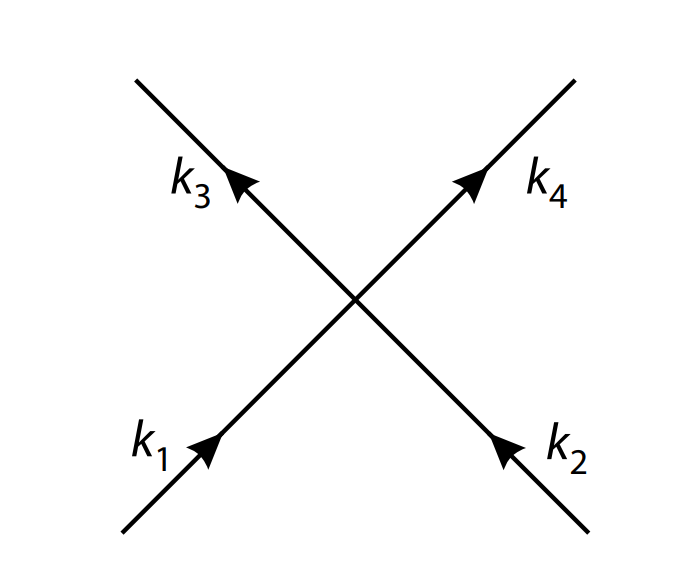
\includegraphics[scale=0.3]{momentum-propagator}
	\caption{From Zee}
\end{figure}
So we have Feynman diagrams for both position and momentum space. Spacetime Feynman diagrams are just literal pictures of what happened. For momentum space Feynman diagrams, here are the rules to calculate the Green's function for a given process:
\begin{enumerate}
	\item Draw a Feynman diagram of the process.
	\item Label each line with a momentum $k$ and associate with it the propagator
	\begin{align}
	\D(k) = \f{i}{k^2 - m^2 + i\epsilon}.
	\end{align}
	Note that we are in momentum space, so the propagator is just this. 
	\item Associate with each interaction vertex (where four lines meet) the coupling 
	\begin{align}
	-i\lambda \hspace{1cm} \text{and} \hspace{1cm}  2\pi^4\delta^{(4)}\lp\sum_i k_i -\sum_j k_j\rp,
	\end{align}
	forcing the sum of momenta $\sum_i k_i$ coming into the vertex to be equal to the sum of momenta $\sum_j k_j$ going out of the vertex. (Note that the act of associating $\lambda$ to an interaction vertex is exactly what we did in the baby problem.)
	\item Momenta associated with internal lines are to be integrated over with the measure $d^4k / (2\pi)^4$, where $k$ denotes the internal/intermediate momentum. Incidentally, this corresponds to the summation over intermediate states in ordinary perturbation theory. 
	\item We have to be careful about symmetry factors. They are the analogs of those numerical factors in the baby problem. As a result, some diagrams are to be multiplied by a symmetry factor such as $1/2$. These come from various combinatorial factors counting the different ways in which the $\delta/\delta J$'s can hit the $J$'s in the multiple integral like \eqref{multi-J}.
	\item We also do not associate a propagator with external lines. 
	\item A delta function for overall momentum conservation is understood. 
\end{enumerate}\qed\\


For example, we can try the diagram we just saw:

\begin{figure}[!htb]
	\centering
	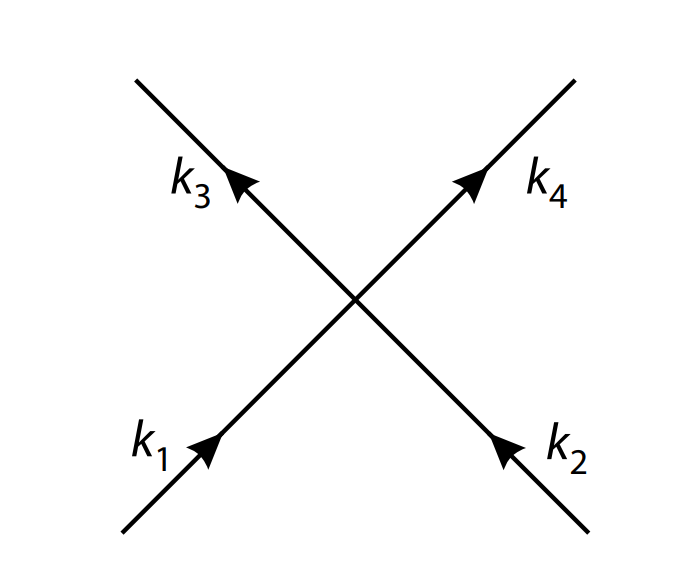
\includegraphics[scale=0.3]{momentum-propagator}
	\caption{From Zee}
\end{figure}

Applying the rules, we obtain
\begin{align}
(-i\lambda)(2\pi)^4\delta^{(4)}(k_1 + k_2 - k_3 - k_4)\prod^4_{a=1}\lp \f{i}{k_a^2 - m^2 + i\epsilon} \rp.
\end{align}

The big multiplicative factor is common to all diagrams in which two mesons scatter into two mesons. So we will just assume it is there and ignore that it is there. This procedure is called ``amputating external legs.'' We also have that in real experiments $k_a^2 = m^2$ since the momentum and mass are equivalent when $c=1$. There are some technical things which we will deal with later. We also see that because momentum must be conserved, we shouldn't worry too much about the delta function either. So same with the other factor, we will just assume it's there and don't write it. \\

With these rules, the amplitude we obtain is denoted by $\mathcal{M}$. For the diagram above, 
\begin{align}
\mathcal{M} = -i\lambda.
\end{align}






















\subsubsection{Birth of particles}



In this section we will describe how two colliding mesons can produce four mesons. 
\begin{figure}[!htb]
	\centering
	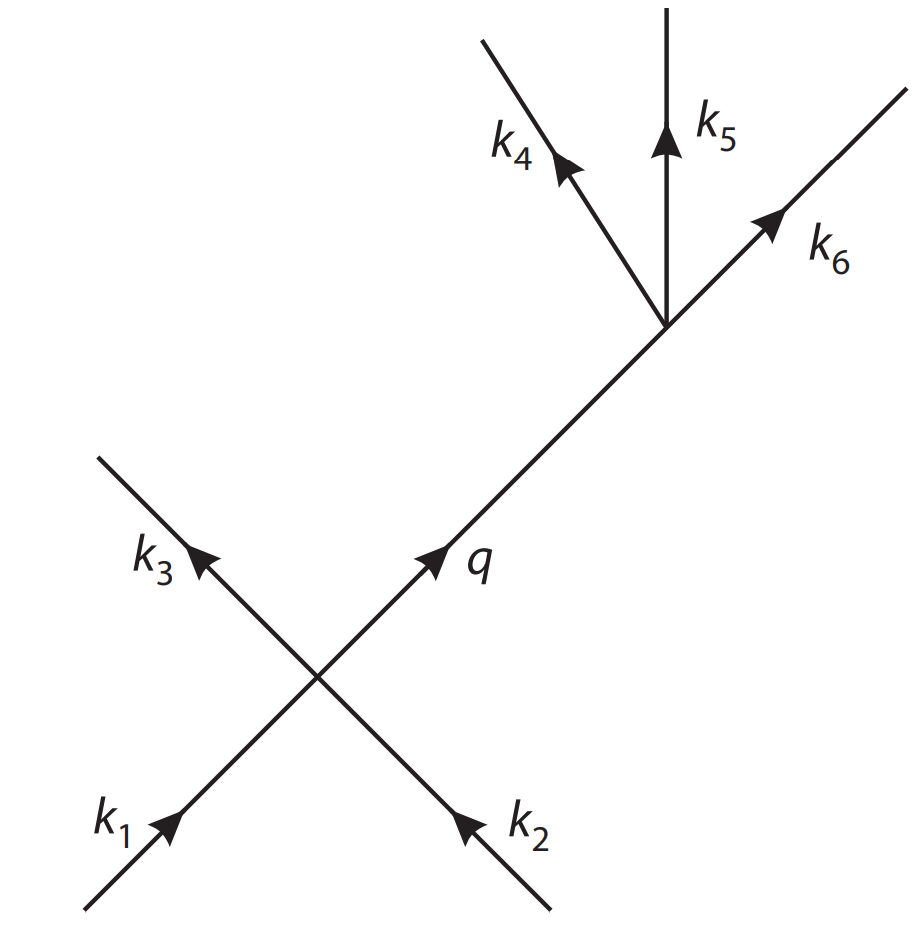
\includegraphics[scale=0.3]{birth}
	\caption{From Zee}
\end{figure}


The process above can occur in $\lambda^2$ perturbation theory. Let us use Feynman's rules to calculate the Green's function/correlation function $G$ for this process. \\

First, the Feynman diagram is already given to us. Good. We would like to calculate the Green's function associated with this diagram.\\

Second, there are $6$ external vertices, so we \textbf{drop} the factor 
\begin{align}
\prod^6_{a=1}\f{i}{k_a^2 - m^2 + i\epsilon},
\end{align}
keeping only the propagator associated with the one internal line, which is
\begin{align}
\f{i}{q^2 - m^2 + i\epsilon}
\end{align} \\

Third, we associate with each interaction vertex a $-i\lambda$. Since there are two of these, we will have a factor of $(-i\lambda)^2$. Next, at the lower vertex we have a factor of $(2\pi)^4\delta^{(4)}\lp k_1 + k_2 - p - k_3 \rp$. At the higher vertex we have a factor of $(2\pi)^4\delta^{(4)}\lp q - k_4 - k_5 - k_6 \rp$. This leaves us with the integrand:
\begin{align}
(-i\lambda)^2 (2\pi)^4\delta^{(4)}\lp k_1 + k_2 - p - k_3 \rp (2\pi)^4\delta^{(4)}\lp q - k_4 - k_5 - k_6 \rp.
\end{align}

Fourth, we integrate the whole term over with the measure $d^p/(2\pi)^4$, since $p$ is the internal momentum here
\begin{align}
(-i\lambda)^2\int \f{d^4 q}{(2\pi)^4} \f{i}{q^2 - m^2 + i\epsilon} (2\pi)^4\delta^{(4)}\lp k_1 + k_2 - p - k_3 \rp \nonumber\\
\hspace{2cm}\times(2\pi)^4\delta^{(4)}\lp q - k_4 - k_5 - k_6 \rp.
\end{align}
Integrals involving delta functions are \textit{very} easy to do. We simply take $q = k_4 + k_5 + k_6$. We should get
\begin{align}
(-i\lambda)^2 \f{i}{(k_4 + k_5 + k_6)^2 - m^2 + i\epsilon} (2\pi)^4\delta^{(4)}(k_1 + k_2 - k_3 - k_4 - k_5 - k_6). 
\end{align}

Finally, the delta function for overall momentum conservation is understood, so 
\begin{align}\label{6-momentum}
\mathcal{M} = (-i\lambda)^2 \f{i}{(k_4 + k_5 + k_6)^2 - m^2 + i\epsilon}
\end{align}
is our answer.\qed











\subsubsection{Cost of not being real}

So what is this relativistic 4-momentum $q = k_4 + k_5 + k_6$? It is the momentum associated with the virtual particle! We notice that $(k_4 + k_5 + k_6)^2$ is not necessarily $m^2$, as it would have to be if the particle were real. The farther the momentum of the virtual particle is from the mass shell $m^2$ the smaller the amplitude, from Eq \eqref{6-momentum}. This makes good sense as the ``cost of not being real.''\\

We can in fact compute Eq \eqref{6-momentum} up to some delta functions and multiplicative factors, just to make sure we understand how the path integral works. But we won't worry about that for now since we have been quite detailed in the previous section. It would be a very good but rather time-consuming exercise.




\subsubsection{Loops and a first look at divergence}

Now, recall from the baby problem that we have both loop and tree diagrams. Loop diagrams are associated with at least a $\lambda$ but no $J$. It is quite similar here in the actual problem. Consider the following Feynman diagram:
\begin{figure}[!htb]
	\centering
	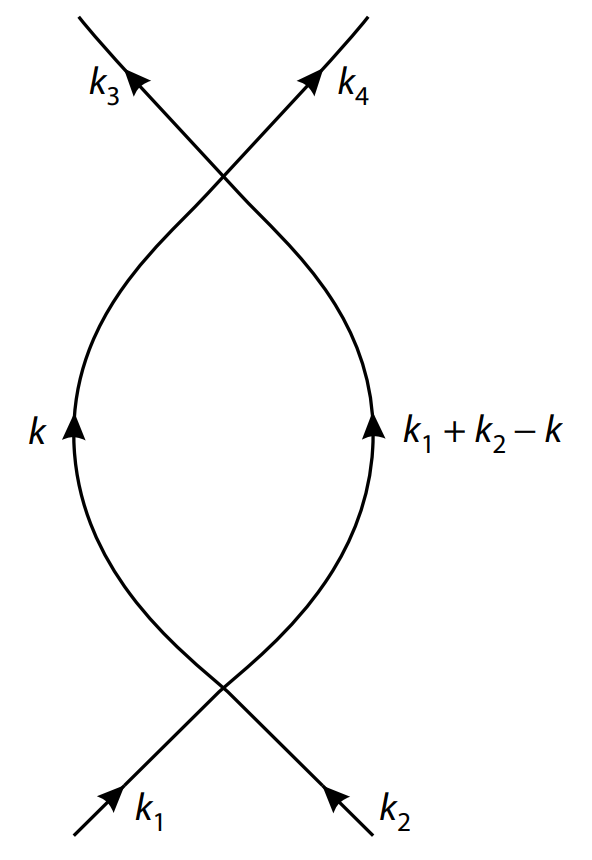
\includegraphics[scale=0.3]{loop-feynman}
	\caption{From Zee}
\end{figure}

We see that there are 2 internal vertices where 4 lines cross. So we get a factor of $(-i\lambda)^2$. We also have 2 factors of internal momentum, after taking into account two delta functions for $k$:
\begin{align}
\f{i}{k^2 - m^2 + i\epsilon} \text{ and } \f{i}{(k_1 + k_2 - k)^2 - m^2 + i\epsilon}.
\end{align}
There is a symmetry factor of $1/2$, since there are two ways this process can occur. We also have some extra factors of $(2\pi)^4$ but we will eventually drop then in the end with one leftover delta function. So the Green's function up to some factor is
\begin{align}
\f{1}{2}(-i\lambda)^2\int \f{d^4k}{(2\pi)^4}\f{i}{k^2 - m^2 + i\epsilon}\f{i}{(k_1 + k_2 - k)^2 - m^2 + i\epsilon}.
\end{align}


This integral blows up only if one of the integrals blow up, i.e., the virtual particle is closest to being real. This is also a cost of not being real. \\

But notice that for large $k$, the integrand goes as $1/k^4$, which means the integral diverges. This is no good! We will come back to this later.\\

Success comes with practice. The more we calculate Feynman diagrams the better we get at doing them by inspection. Here is another example. I won't go into detail what the steps involved are, but we can convince ourselves that the Green's function associated with the following Feynman diagram
\begin{figure}[!htb]
	\centering
	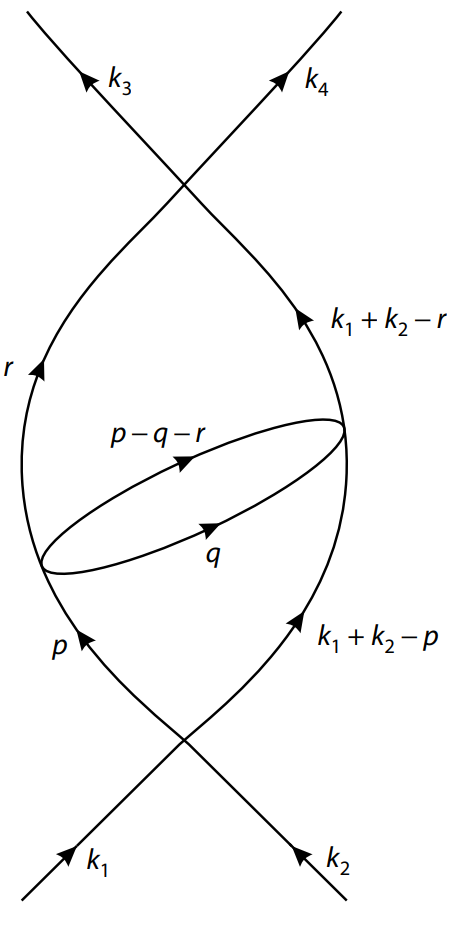
\includegraphics[scale=0.3]{loop-2}
	\caption{From Zee}
\end{figure}

up to symmetry factors and other factors that we don't write down is 
\begin{align}
&(-i\lambda)^4 \int \f{d^4p}{(2\pi)^4}\f{d^4q}{(2\pi)^4}\f{d^4r}{(2\pi)^4} \f{i}{p^2-m^2 +i\epsilon}\f{i}{(k_1+k_2-p)^2-m^2 +i\epsilon}\nonumber\\ &\,\times\f{i}{q^2-m^2 +i\epsilon}\f{i}{(p-q-r)^2-m^2 +i\epsilon}\f{i}{r^2-m^2+i\epsilon}\f{i}{(k_1+k_2-r)^2-m^2 +i\epsilon}
\end{align}





\subsubsection{Vacuum fluctuations}


Let us revisit the self-interaction term we neglected in the full expression 
\begin{align}
i\lambda \int_w \lp \f{\delta}{\delta J(w)} \rp^4 \bigintss^{(8)}  \D_{ae}\D_{bf}\D_{cg}\D_{dh}J_aJ_bJ_cJ_dJ_eJ_fJ_gJ_h
\end{align}
for the Green's function in first order of $\lambda$. Recall that we only kept terms without $\D_{ww}\D_{ww}$ when the $\delta/\delta J(w)$ could have hit $J_c, J_d, J_h, J_g$, resulting in
\begin{align}
-i\lambda \iiiint \D_{ae}\D_{bf} J_a J_b J_eJ_f \lp \int_w \D_{ww}\D_{ww} \rp.
\end{align}
How exactly does this happen? Well,
\begin{align}
\f{\delta}{\delta J(w)}J_j = \delta(x_j - w),
\end{align}
setting $w \to c,d,g,h$, creating $\D_{ww}\D_{ww}$. In this case, the coefficient of $J(x_1)J(x_2)J(x_3)J(x_4)$ us then
\begin{align}
\D_{13}\D_{24} (-i\lambda)\int_w \D_{ww}\D_{ww}
\end{align}
plus other terms by permuting. Because the subscripts of $\D_{13}$ and $\D_{24}$ don't overlap (obviously), we get disconnected diagrams. Also, because we have $\D_{ww}\D_{ww}$, we also get a self-interaction. The associated spacetime Feynman diagram is then
\begin{figure}[!htb]
	\centering
	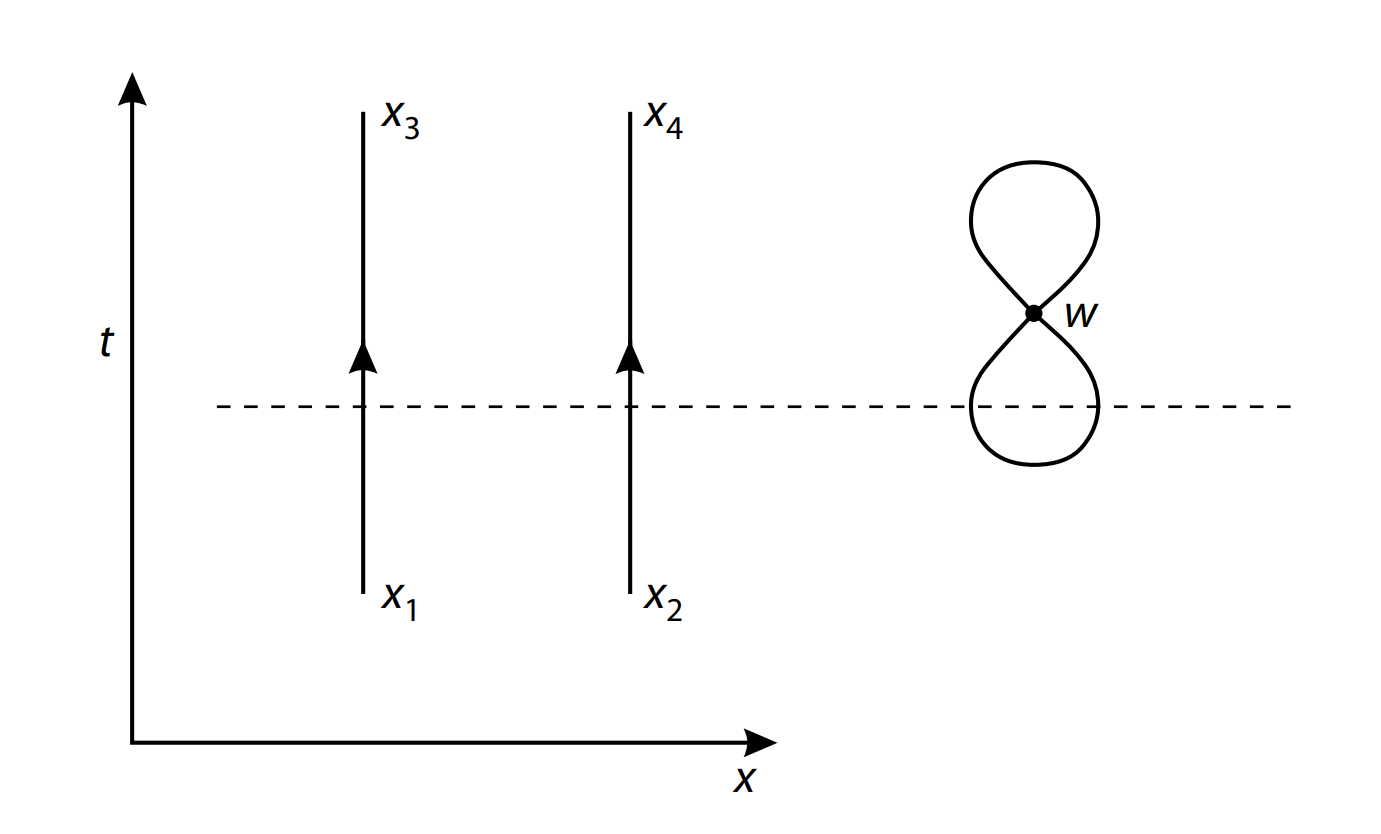
\includegraphics[scale=0.3]{self-int}
	\caption{From Zee}
\end{figure}


Let's describe the underlying physical process: The source at $x_1$ produces a particle that propagates freely without any interaction to $x_3$, where it disappears. A similar thing happen to a particle starting at $x_2$ and ending at $x_4$. These two particles don't interact (disconnected). Now, somewhere off at the point $w$, which could really be \textit{anywhere}, there was an interaction with amplitude $-i\lambda$. This is known as a \textbf{vacuum fluctuation}.\\


Now, when quantum mechanics and special relativity comes together, particles inevitably pop in and out of the vacuum. They could also even interact before vanishing again into the vacuum. From the figure, we see that in the far past, the universe has no particles. Then there are two, then four, then two, then none. We will deal with these fluctuations in better details later. \\

Note that we have seen vacuum fluctuations in the Feynman diagrams in our baby and child problems. We just didn't talk about them!











\newpage









\subsection{Canonical Quantization}




\subsubsection{Heisenberg \& Dirac}


Consider a classical Lagrangian for a single particle
\begin{align}
\boxed{\lag = \f{1}{2}\dot{q}^2 - V(q)}
\end{align}
setting the mass to 1. The canonical momentum is defined by
\begin{align}
p \equiv \f{\delta \lag }{\delta \dot{q}}.
\end{align}
The Hamiltonian is then given by
\begin{align}\label{hamilton}
\ham = p\dot{q} - \lag = \f{p^2}{2} + V(q).
\end{align}

In the Heisenberg formulation, position $q(t)$ and momentum $p(t)$ are promoted to operators which follow the commutation relations:
\begin{align}
\boxed{[p,q] = -i}
\end{align}
where we have set $\hbar = c = 1$. Operators evolve in time according to Heisenberg's equation of motion
\begin{align}
\boxed{\f{dp}{dt} = i[\ham , p] = -\p_q V(q)} \text{ and } \boxed{\f{dq}{dt} = i[\ham , q] = p}
\end{align}
where we have assumed these operators are not explicitly time-dependent. \\

Any operator $O$ constructed out of $p,q$ evolves according to 
\begin{align}
O(t) = e^{i\ham t} O(0) e^{-i\ham t}.
\end{align} 
In particular, consider the following operator:
\begin{align}
a \equiv \f{1}{\sqrt{2w}}\lp wq + ip \rp
\end{align}
defined with some parameter $w$. From the commutation relations between $q$ and $p$, we have that
\begin{align}
\boxed{[a,a^\dagger] = 1}
\end{align}


The evolution of this operator is given by
\begin{align}
\boxed{\f{da}{dt} = i\lb\ham, \f{1}{\sqrt{2w}}(wq + ip)\rb = -i\f{w}{2}\lp ip + \f{1}{w}V'(q) \rp}
\end{align}

The $a$ operator is called the \textit{lowering operator}, defined such that
\begin{align}
\boxed{a\ket{0} = 0}
\end{align}

In the special case of the harmonic oscillator, $V(q) = w^2 q^2/2$, we have that 
\begin{align}
\f{da}{dt} &= -iw a\\
\lag &= \f{1}{2}\dot{q}^2 - \f{1}{2}w^2 q^2\\
\ham &= \f{1}{2}(p^2 + w^2 q^2) = w\lp a^\dagger a + \f{1}{2} \rp\\
[p, q] &= -i.
\end{align}



In general, with multi-particle systems,
\begin{align}
\lag &= \sum_a^N \f{1}{2}\dot{q}_a^2 - V(q_1, q_2, \dots, q_N)\\
p_2 &= \f{\delta \lag}{\delta \dot{q}_a}\\
[p_a(t), q_b(t)] &= -i\delta_{ab}.
\end{align}
where $p_a, q_b$ can be written in terms of the lowering and raising operators. \\


We can also generalize this Lagrangian even further in field theory in $D$-dimensional space:
\begin{align}
\boxed{L = \int d^Dx\, \underbrace{\lc \f{1}{2}[\dot{\phi}^2 - (\grad{\phi})^2 - m^2 \phi^2] - u(\phi) \rc}_{\lag}}
\end{align}
where $u(\phi)$ denotes anharmonic terms. \\

In this case, the canonical momentum density conjugate to the field $\phi(\vec{x},t)$ is given by
\begin{align}
\boxed{\pi (\vec{x} ,t) = \f{\delta \lag}{\delta\dot{\phi}(\vec{x},t)} = \p_0 \phi(\vec{x},t) }
\end{align}
And it follows that the commutation relation (at equal times) now reads
\begin{align}
\boxed{\lb \pi(\vec{x},t), \phi(\vec{x}',t) \rb = \lb \p_0 \phi(\vec{x},t), \phi(\vec{x}',t) \rb = -i\delta^{(D)}(\vec{x} - \vec{x}')}
\end{align}


The Hamiltonian can be found from the Lagrangian (density) similar to Eq. $\eqref{hamilton}$ via 
\begin{align}
H = \int d^D x\, \lc \pi(\vec{x},t) \underbrace{\p_0\phi(\vec{x},t)}_{\pi(\vec{x},t)} - \lag \rc = \int d^Dx\, \lc \f{1}{2}\lb\pi^2 + (\grad{\phi})^2 + m^2 \phi^2\rb     + u(\phi) \rc.
\end{align}

When we don't have any anharmonic terms, i.e. $u(\phi) = 0$, we recover the harmonic oscillator. In this case, we have a free scalar field theory, where $\phi$ solves the Klein-Gordon equation:
\begin{align}
(\p^2 + m^2)\phi  = 0
\end{align}
where
\begin{align}
\p^2 = \f{\p^2}{\p t^2} - \grad.
\end{align}
The Klein-Gordon equation is obtained from varying the Lagrangian with respect to the field. \\

We can verify that the solution to this Klein-Gordon equation has the form
\begin{align}
\boxed{\phi(\vec{x},t) = \int \f{d^D k}{\sqrt{(2\pi)^D 2 w_k}} \lb a(\vec{k})e^{-i(w_k t - \vec{k}\cdot\vec{x})} + a^\dagger(\vec{k})e^{i(w_k t - \vec{k}\cdot \vec{x})} \rb}
\end{align}
where 
\begin{align}
w_k = \sqrt{\vec{k}^2 + m^2}.
\end{align}
The factor $\sqrt{2w_k}^{-1}$ is chosen so that we have
\begin{align}
[a(\vec{k}), a^\dagger(\vec{k})] = \delta^{(D)}(\vec{k} - \vec{k}'),
\end{align}
which implies the correct commutation relation for the field and canonical momentum 
\begin{align}
[\p_0 \phi(\vec{x}, t), \phi(\vec{x}', t)]  = -i\delta^{(D)}(\vec{x} - \vec{x}').
\end{align}





In quantum mechanics, the ground state or vacuum is denoted by $\ket{0}$, following the condition
\begin{align}
a(\vec{k})\ket{0} = 0.
\end{align}
Any single particle state with momentum $\vec{k}$ is given by
\begin{align}
a^\dagger(\vec{k})\ket{0} = \ket{k}.
\end{align}
Consider the expectation value $\bra{0}\phi(\vec{x},t)\ket{k}$. We can compute this
\begin{align}
&\bra{0}\phi(\vec{x},t)\ket{k} \nonumber\\
= &\bra{0}\int \f{d^D k'}{\sqrt{(2\pi)^D 2 w_k'}} \lb a(\vec{k'})e^{-i(w_{k'} t - \vec{k}'\cdot\vec{x})} + a^\dagger(\vec{k}')e^{i(w_{k'} t - \vec{k}'\cdot \vec{x})} \rb \lp a^\dagger(k)\ket{0} \rp \nonumber \\ 
= &\bra{0}\int \f{d^D k'}{\sqrt{(2\pi)^D 2 w_k'}} \lb a(\vec{k'}) a^\dagger(\vec{k})e^{-i(w_{k'} t - \vec{k}'\cdot\vec{x})} + \underbrace{a^\dagger(\vec{k}')a^\dagger(\vec{k})e^{i(w_{k'} t - \vec{k}'\cdot \vec{x})} }_{\text{makes an orthogonal vector to $\ket{0} \forall k$}}\rb\ket{0} \nonumber \\ 
= &\bra{0}\int \f{d^D k'}{\sqrt{(2\pi)^D 2 w_k'}} \lb a(\vec{k'}) a^\dagger(\vec{k})e^{-i(w_{k'} t - \vec{k}'\cdot\vec{x})}\rb\ket{0} \nonumber \\ 
= &\int \f{d^D k'}{\sqrt{(2\pi)^D 2 w_k'}} \lb \bra{0} a(\vec{k'}) a^\dagger(\vec{k})\ket{0}e^{-i(w_{k'} t - \vec{k}'\cdot\vec{x})}\rb \nonumber \\ 
= &\int \f{d^D k'}{\sqrt{(2\pi)^D 2 w_k'}} \lb e^{-i(w_{k'} t - \vec{k}'\cdot\vec{x})}\rb \delta^{(D)}(\vec{k} - \vec{k}') \nonumber\\
= & \boxed{\f{1}{\sqrt{(2\pi)^D 2w_k}}e^{-i(w_k t - \vec{k}\cdot\vec{x})}}
\end{align}



To make contact with the path integral formulation let us evaluate $\bra{0}\phi(\vec{x},t)\phi(\vec{0},0)\ket{0}$ for $t > 0$. Before attempting this by writing the entire expression out, we will notice that of the four possible terms $a^\dagger a^\dagger$, $a^\dagger a$, $a a^\dagger$, and $aa$ in the product of the two fields only $a a^\dagger$ survives because of orthogonality relations and the fact that we're staring out with the ground state. With this, we will proceed:
\begin{align}
  &\bra{0}\phi(\vec{x},t)\phi(\vec{0},0)\ket{0} \nonumber\\
= &\iint \f{d^D k}{\sqrt{(2\pi)^D 2w_k}} \f{d^D k'}{\sqrt{(2\pi)^D 2w_{k'}}}
\bra{0}\lc a(\vec{k})e^{-i(w_k t - \vec{k}\cdot\vec{x})} + a^\dagger(\vec{k})e^{i(w_k - \vec{k}\cdot\vec{x})} \rc \lc a(\vec{k}') + a^\dagger(\vec{k}') \rc\ket{0} \nonumber\\
= &\iint \f{d^Dk \,d^Dk'}{(2\pi)^D (2w_k)(2w_{k'})}e^{-i(w_k t - \vec{k}\cdot\vec{x})}\bra{0}a(\vec{k})a^\dagger(\vec{k}')\ket{0}\nonumber\\
= &\iint \f{d^Dk \,d^Dk'}{\sqrt{(2\pi)^D (2w_k)(2w_{k'})}}e^{-i(w_k t - \vec{k}\cdot\vec{x})}\delta^{(D)}(\vec{k} - \vec{k}')\nonumber\\
= &\iint \f{d^Dk \,d^Dk'}{\sqrt{(2\pi)^{2D} (2w_k)(2w_{k'})}}e^{-i(w_k t - \vec{k}\cdot\vec{x})}\delta^{(D)}(\vec{k} - \vec{k}')\nonumber\\
= &\boxed{\int \f{d^D k}{(2\pi)^{D} 2w_k}e^{-i(w_k t - \vec{k}\cdot\vec{x})}}
\end{align}


With this, if we define the time-ordering product 
\begin{align}
\boxed{T[\phi(x)\phi(y)] = \theta(x^0 - y^0) \phi(x)\phi(y) + \theta(y^0 - x^0)\phi(y)\phi(x)}
\end{align}
then we have
\begin{align}
  &\bra{0}T[\phi(\vec{x},t)\phi(\vec{0},0)]\ket{0} \nonumber\\
= &\bra{0}  \theta(t)\phi(x)\phi(0) + \theta(-t)\phi(0)\phi(x)   \ket{0} \nonumber\\
= &\bra{0}  \theta(t)\phi(x)\phi(0)\ket{0} + \bra{0}\theta(-t)\phi(0)\phi(x)  \ket{0} \nonumber\\
= & \boxed{\int \f{d^D k}{(2\pi)^D 2w_k}\lb \theta(t)e^{-i(w_k t - \vec{k}\cdot\vec{x})} + \theta(-t)e^{i(w_k t - \vec{k}\cdot\vec{x})} \rp}
\end{align}

where
\begin{align}
\bra{0} \phi(x)\phi(0) \ket{0} &= \int \f{d^D k}{(2\pi)^D 2w_k}e^{-i(w_k t - \vec{k}\cdot\vec{x})} \\ 
\bra{0} \phi(0)\phi(x) \ket{0} &= \int \f{d^D k}{(2\pi)^D 2w_k}e^{+i(w_k t - \vec{k}\cdot\vec{x})}
\end{align}
which we can check by inspection. Comparing this result to Eq. \eqref{propag}, which we will repeat here:
\begin{align}
\D(x) = \f{-i}{(2\pi)^3}\int \f{d^3k}{ 2 w_k} \lb e^{-i[w_kt - \vec{k}\cdot\vec{x}]}\theta(t) + e^{i[w_kt - \vec{k}\cdot\vec{x} ]}\theta(-t)\rb,
\end{align}
we immediately see that
\begin{align}
\boxed{\bra{0}T[\phi(\vec{x},t)\phi(\vec{0},0)]\ket{0} = i\D(x) = G^{(2)}(x,0)}
\end{align}

This nicely connects quantum mechanics to the path integral formalism. \\

The moral here is that we always create before we annihilate, not the other around. This is a form of causality as formulated in quantum field theory. 






\subsubsection{Scattering amplitude}


In this section we will show how the invariant scattering amplitude $\mathcal{M}$ arises from this formalism. Suppose we would like to evaluate the quantity:
\begin{align}
\boxed{\bra{\vec{k_3}\vec{k_4}}e^{-iH T}\ket{\vec{k_1} \vec{k_2}} = \bra{\vec{k_3}\vec{k_4}}e^{i \int d^4x\, \lag(x) }\ket{\vec{k_1} \vec{k_2}} }
\end{align} 
for the following meson scattering process
\begin{align}
\vec{k_1} + \vec{k_2} \to \vec{k_3}+ \vec{k_4}
\end{align}
in order $\lambda$, with the anharmonic term $u(\phi) = \lambda \phi^4 / 4!$. The ``sandwiched'' term is given by
\begin{align}
&\exp\lc i \int d^4x\,\f{1}{2}\p^\mu \phi \p_\mu \phi - \f{1}{2}m^2\phi^2 - \f{\lambda}{4!}\phi^4(x) \rc
\end{align}
Next, let us expand in $\lambda$ and collect only the term in order $\lambda$. This term is 
\begin{align}
\int d^4x\,\lb i\f{\lambda}{4!}\phi^4(x) \rb \times \exp\lc -i \int d^4x\,\f{1}{2}\lb \p^\mu \phi \p_\mu \phi - m^2\phi^2 \rb \rc.
\end{align}
Next, recall from the \textbf{Perturbative Field Theory} section that we can integrate the integral in the exponent above by parts and show that 
\begin{align}
&\exp\lc -i \int d^4x\,\f{1}{2}\lb \p^\mu \phi \p_\mu \phi - m^2\phi^2 \rb \rc \nonumber\\
= &\exp\lc -i \int d^4x\,\f{-1}{2}\phi\lb \underbrace{ \square + m^2}_{A} \rb\phi \rc \nonumber\\
= &\exp\lc i \int d^4x\,\lp\f{1}{2}\phi A \phi\rp \rc.
\end{align}
Now, because $\phi$ is the solution to the free field (Klein-Gordon) equation, we must have that
\begin{align}
(\square + m^2)\phi = A\phi = 0 \implies \exp\lc -i \int d^4x\,\f{1}{2}\lb \p^\mu \phi \p_\mu \phi - m^2\phi^2 \rb \rc \equiv 1. 
\end{align}
Thus,
\begin{align}
\boxed{\bra{\vec{k_3}\vec{k_4}}e^{-iH T}\ket{\vec{k_1} \vec{k_2}} \approx \lp -i\f{\lambda}{4!} \rp\int d^4x \, \bra{\vec{k_3}\vec{k_4}}\phi^4(x)\ket{\vec{k_1} \vec{k_2}}}
\end{align}
  
  
How do we actually calculate this? There is some similarity between what we have done and what we have here. Before, we have a product of two fields sandwiched between the ground states. Now, we have four, sandwiched between two four-particle states. In order to correct describe the picture, we need to annihilate $\ket{\vec{k_1}}$ and $\ket{\vec{k_2}}$ then create $\ket{\vec{k_3}}$ and $\ket{\vec{k_4}}$. Thus we look for the term $a^\dagger(\vec{k_4}) a^\dagger(\vec{k_3})a(\vec{k_2})a(\vec{k_1})$. The $a(\vec{k_1})$ term could come from any of the four fields $\phi$. The $a(\vec{k_2})$ terms cold come from any of the leftover three fields, and so on. In the end, we have $4!$ of $a^\dagger(\vec{k_4}) a^\dagger(\vec{k_3})a(\vec{k_2})a(\vec{k_1})$ terms. This $4!$ cancels with the term in the denominator. The exponential corresponding to this term is 
\begin{align}
e^{ i \lp (w_4 t - \vec{k}_4 \cdot \vec{x}) + (w_3 t - \vec{k}_3 \cdot \vec{x}) - (w_2 t - \vec{k}_2 \cdot \vec{x}) - (w_1 t - \vec{k}_1 \cdot \vec{x})\rp } \equiv e^{i (k_3 + k_4 - k_1 - k_2)\cdot x}.
\end{align}
So, the matrix element is 
\begin{align}
\lp \prod^4_{\alpha = 1} \f{1}{\sqrt{(2\pi)^D 2 w_\alpha}} \rp \int d^4x\, e^{i (k_3 + k_4 - k_1 - k_2)\cdot x} 
\end{align}
Finally, recall that
\begin{align}
\delta^{(4)}(x - y) = \F[1](x-y) \f{1}{(2\pi)^4}\int d^4p \, e^{i(x-y)p},
\end{align}
so we have the full amplitude: 
\begin{align}
\boxed{\lp -i\lambda \rp \lp \prod^4_{\alpha = 1} \f{1}{\sqrt{(2\pi)^D 2 w_\alpha}} \rp (2\pi)^4 \delta^{(4)}(k_3 + k_4 - k_2 - k_1)}
\end{align}
where we recall that $\mathcal{M}(f \leftarrow i) = -\lambda$.\\

It is conventional to refer to 
\begin{align}
S_{fi} = \bra{f}e^{-iHT}\ket{i}
\end{align}
as the matrix elements of the $S$-matrix. From here, we can define the transition matrix $T$ by 
\begin{align}
S \equiv I + iT \iff S_{fi} = \delta_{fi} + iT_{fi}.
\end{align}
With this, and expressing the change in momentum in general as the sum of final minus the sum of initial momenta, we get
\begin{align}
\boxed{iT_{fi} = (2\pi)^4 \delta^{(4)}\lp \sum_f k - \sum_i k \rp \lp \prod^4_{\alpha = 1} \f{1}{\sqrt{(2\pi)^D 2 w_\alpha}} \rp \mathcal{M}(f \leftarrow i)}
\end{align}




\subsubsection{Energy of the vacuum}


In this section we will find the expectation value $\bra{0}H\ket{0}$ in the free scalar field theory where we have constructed the Hamiltonian from the Lagrangian:
\begin{align}
H = \pi^2 + (\grad{\phi})^2 + m^2 \phi^2.
\end{align}

Recall that we have computed $\phi$:
\begin{align}
\phi(\vec{x},t) = \int \f{d^D k}{\sqrt{(2\pi)^D 2 w_k}} \lb a(\vec{k})e^{-i(w_k t - \vec{k}\cdot\vec{x})} + a^\dagger(\vec{k})e^{i(w_k t - \vec{k}\cdot \vec{x})} \rb.
\end{align}
It follows that
\begin{align}
\pi^2(\vec{x},t) &= [\p_0 \phi(\vec{x},t)]^2 = w_k^2 \phi^2(\vec{x},t)\nonumber\\
(\grad{\phi})^2 &= \vec{k}^2 \phi^2(\vec{x},t) \nonumber.
\end{align}
So we only have to look at $\bra{0}\phi(\vec{x},t)\phi(\vec{x},t)\ket{0}$:
\begin{align}
\bra{0}\phi(\vec{x},t)\phi(\vec{x},t)\ket{0} &=  
\end{align}


We also have that
\begin{align}
&\bra{0}\phi^2(\vec{x},t)\ket{0} \nonumber\\
= &\bra{0}\phi(\vec{x},t)\phi(\vec{x},t)\ket{0} \nonumber\\
= &\bra{0} \lp \int \f{d^Dk}{\sqrt{(2\pi)^D 2w_k}} \lc a(\vec{k})e^{ik\cdot x} + a^\dagger(\vec{k})e^{-ik\cdot x} \rc \rp^2   \ket{0} \nonumber\\
= &\iint \f{d^D k\,d^Dk'}{\sqrt{(2\pi)^{2D}(2w_k)(2w_k')}}\bra{0} \lc a(\vec{k})e^{ik\cdot x} + a^\dagger(\vec{k})e^{-ik\cdot x}  \rc \lc a(\vec{k'})e^{ik'\cdot x} + a^\dagger(\vec{k'})e^{-ik'\cdot x}  \rc \ket{0} \nonumber\\
= &\iint \f{d^D k\,d^Dk'}{\sqrt{(2\pi)^{2D}(2w_k)(2w_k')}}\underbrace{\bra{0} a(\vec{k})a^\dagger(\vec{k}')e^{i(k-k')\cdot x} \ket{0}}_\delta \nonumber\\
= &\iint \f{d^D k\,d^Dk'}{\sqrt{(2\pi)^{2D}(2w_k)(2w_k')}} \delta^{(D)}(k - k')\nonumber\\
= & \int \f{d^D k}{(2\pi)^D 2w_k}.
\end{align}
Putting this together, we find
\begin{align}
\bra{0}H\ket{0} &= \int d^Dx\f{1}{2}\bra{0} \lp \pi^2 + (\grad{\phi})^2 + m^2 \phi^2 \rp\ket{0} \nonumber\\
&= \underbrace{\int d^Dx}_{V}\,  \int \f{d^D k}{(2\pi)^D 2w_k} \f{1}{2} (w_k^2 + \vec{k}^2 + m^2)   \nonumber\\
&= V  \int \f{d^D k}{(2\pi)^D 2w_k} \f{1}{2} (w_k^2 + \underbrace{\vec{k}^2 + m^2}_{w_k^2}) \nonumber\\
&= V  \int \f{d^D k}{(2\pi)^D} \f{1}{2}w_k.
\end{align}
Once $\hbar$ is restored, we get
\begin{align}
\boxed{\bra{0}H\ket{0} = V  \int \f{d^D k}{(2\pi)^D} \f{1}{2}\hbar w_k}
\end{align}
where $V$ the volume of the space. \\


We immediately recognize this as the zero-point energy of the harmonic oscillator integrated over all momentum modes $k$ and over all space. However, we should worry here because this integral over $k$ clearly diverges. However, in reality, we always measure relative to the vacuum, i.e., we are often interested in 
\begin{align}
H - \bra{0}H\ket{0}.
\end{align}
Thus, we won't have to worry about getting infinities here.











\subsubsection{Complex scalar field}

In the previous section, our field is hermitian (or ``real''). In this section, we will look at the formalism for a complex scalar field governed by the Lagrangian density:
\begin{align}
\boxed{\lag = \p \phi^\dagger \p \phi - m^2 \phi^\dagger \phi}
\end{align} 

According to Heisenberg, the canonical momentum is given by
\begin{align}
{\pi(\vec{x},t) = \f{\delta \lag}{\delta \dot{\phi}(\vec{x},t)} = \p_0 \phi^\dagger(\vec{x},t)}
\end{align}
and so 
\begin{align}
{[\pi(\vec{x},t), \phi(\vec{x}',t)] = -i\delta^{(D)}(\vec{x} - \vec{x}')}
\end{align}
just as before. Similarly, we can show that 
\begin{align}
{\pi'(\vec{x},t) = \f{\delta \lag}{\delta \dot{\phi}^\dagger(\vec{x},t)} = \p_0 \phi(\vec{x},t)}
\end{align}

Varying the Lagrangian with respect to the (conjugate of the) field, we get two Klein-Gordon equations:
\begin{align}
{(\square + m^2)\phi = 0; \hspace{0.5cm}(\square + m^2)\phi^\dagger = 0}
\end{align}
 
The Fourier expansion is similar to what we've seen before. However, because $\phi$ is no longer hermitian, we are required to use two independent sets of creation and annihilation operators $(a,a^\dagger)$ and $(b, b^\dagger)$:
\begin{align}
\boxed{\phi(\vec{x},t) = \int \f{d^Dk}{\sqrt{(2\pi)^D 2w_k}}\lb a(\vec{k})e^{-i(w_k t - \vec{k}\cdot\vec{x})} + b^\dagger(\vec{k}) e^{i(w_k t - \vec{k}\cdot\vec{x})}\rb}
\end{align}
The interpretation here is that the particle created by $a^\dagger$ and the particle created by $b^\dagger$ are antiparticles. 


















\newpage










\section{The Dirac Equation, Spinors, \& QED    } 






\subsection{Review \& Introduction}

The four dimensional del operator is given by
\begin{align}
\p_\mu = \lp \f{1}{c}\p_t, \p_x ,\p_y, \p_x \rp.
\end{align}
With a Minkowskian associated metric
\begin{align}
\eta_{\mu\nu} = \text{diag}(1,-1,-1,-1),
\end{align}
the Laplacian becomes the d'Alembertian
\begin{align}
\square \equiv \p_\mu \p^\mu = \p^\mu \p_\mu = \eta_{\mu\nu}\p^\mu \p^\nu = \f{1}{c^2}\p_t^2 - \p_x^2 - \p_y^2 - \p_z^2.
\end{align}
When we do quantum field theory, $c\to 1$ so as to be ``natural,'' so
\begin{align}
\square \to \p_t^2 - \p_x^2 - \p_y^2 - \p_z^2.
\end{align}

The non-relativistic Schr\"{o}dinger equation is given by
\begin{align}
\lp\f{-\hbar^2}{2m}\laplacian + U\rp \psi = i\hbar \p_t \psi.
\end{align}
In the natural units, $\hbar = c= 1$, so 
\begin{align}
i\p_t \psi = \lp -\f{1}{2m}\laplacian + U \rp\psi.
\end{align}

The free particle ($U=0$) solution is 
\begin{align}
\psi(\vec{x},t) \propto e^{iEt}\psi(\vec{x}).
\end{align}
For a four-current of the form
\begin{align}
J^\mu = (c\rho, \vec{j}) = (\rho, \vec{j}),
\end{align}
the probability density is 
\begin{align}
\rho = \abs{\psi(x)}^2.
\end{align}
and the 3-current density is
\begin{align}
\vec{j} = -\f{i}{2m}\lp \psi^*\grad{\psi} - \psi \grad{\psi^*} \rp.
\end{align}
These quantities are related via the continuity equation, which is a statement about the conservation of 4-current in spacetime, i.e., $j^\mu$ is divergenceless.
\begin{align}
\p_\mu J^\mu = 0 \iff \p_t \rho + \div{\vec{j}} = 0.
\end{align}

We see that the SE is first order in the time derivative but second order in the space derivative. This is problematic in relativistic theories, since space and time should treated as equivalent. 






\subsubsection{The Klein-Gordon Equation \& Its problem}



For a relativistic particle, the energy-momentum relationship is
\begin{align}
p\cdot p = p_\mu p^\mu = E^2 - \abs{\vec{p}}^2 = m^2.
\end{align}

If we promote energy and momentum to operators and use
\begin{align}
\hat{E} = i\hbar \p_t = i\p_t
\end{align}
and
\begin{align}
\hat{p} = -i\hbar \grad = -i\grad
\end{align}
then we get the Klein-Gordon equation
\begin{align}
(\square + m^2)\psi = 0 \iff \lp -\p_t^2 + \laplacian \rp\psi = m^2 \phi
\end{align}
whose free particle solutions $m^2 = 0 $ are plane waves:
\begin{align}
\psi \propto e^{-ip\cdot x} = e^{-i(Et - \vec{p}\cdot\vec{x})}.
\end{align}

As we have already seen (many many times!), the Klein-Gordon equation successfully describes \textbf{spin 0 particles} in relativistic quantum field theory. However, problems arise with the interpretation of the positive and negative energy solutions:
\begin{align}
E = \pm \sqrt{p^2 + m^2}.
\end{align}


The problems with the Klein-Gordon equation led Dirac to search for an alternative
relativistic wave equation in 1928, in which the time and space derivatives are first
order.























\subsubsection{The Dirac Equation}

\textit{This section is inspired by Freeman Dyson's \href{https://arxiv.org/pdf/quant-ph/0608140.pdf}{\underline{notes}} from 1951, the \href{http://www.smallperturbation.com/physics-proof}{\underline{proof}} by fellow internet user Small Perturbation, and various other online sources. }\\


Dirac (1928) was looking for a covariant wave equation that was first-order in spacetime. But he also wanted an equation whose solution solves the Klein-Gordon equation (at least component-wise). \\

Suppose this new equation has the form
\begin{align}
i\p_t \psi = \beta m \psi - i {\alpha} \cdot \grad{\psi} \equiv \ham_{\text{Dirac}}\psi.
\end{align}

Since any $\psi$ that solves the Dirac equation also solves the KG equation, we must have after separating the time and space pieces:
\begin{align}
-\p_t^2 \psi &= \beta mi \p_t\psi  + \p_t (\alpha\cdot \grad)\psi\nonumber\\
&= \beta mi \p_t \psi + {\alpha}\cdot \grad{\p_t \psi} \nonumber\\
&= \beta m \lc \beta m \psi - i(\alpha \cdot \grad)\psi  \rc  + {\alpha}\cdot \grad{\p_t \psi}\nonumber\\
&= \beta^2 m^2 \psi  - (im)\beta (\alpha \cdot \grad)\psi + (\alpha \cdot \grad)(\p_t \psi) \nonumber\\
&= \beta^2 m^2 \psi  - (im)\beta (\alpha \cdot \grad)\psi + (\alpha \cdot \grad) \lc -i \beta m \psi - i(\alpha \cdot \grad)\psi  \rc \nonumber\\
&= \beta^2 m^2 \psi - (im)[\alpha \cdot\beta + \beta \cdot \alpha ]\grad{\psi} - (\alpha \cdot\grad)^2\psi \nonumber\\
&= -\laplacian{\psi} + m^2 \psi
\end{align}



This means
\begin{align}
\begin{cases}
\beta \cdot \alpha + \alpha \cdot\beta = 0\\
\beta^2 = 1\\
(\alpha \cdot \grad)^2 = \laplacian.
\end{cases}
\end{align}



So we must have that 
\begin{align}
\begin{cases}
\beta^2 = \alpha_x^2 = \alpha_y^2 = \alpha_z^2 = \mathbb{I}\\
 \alpha_j \beta + \beta\alpha_j  = \alpha_j \alpha_k + \alpha_k \alpha_j = \mathbb{O} \hspace{0.5cm}\forall j\neq k = x,y,z.
\end{cases} 
\end{align}



Thus we could not possibly factorize the 2nd order equation into two first-order operators involving ordinary numbers. But we can do it with matrices. \\

\textbf{Lemma:} The $\beta, \alpha_j$ matrices are at least $4\times 4$.\\

\textit{Proof:} We introduce new matrices defined by:
\begin{align}
&\gamma^0 \leftarrow \beta\\
&\gamma^j \leftarrow \beta\alpha_j\hspace{1cm} j =1,2,3.
\end{align}
With this, we are able to combine all of the above conditions into a single statement:
\begin{align}
\boxed{\{\gamma^\mu, \gamma^\nu\} = \gamma^\mu \gamma^\nu + \gamma^\nu\gamma^\mu = 2\eta^{\mu\nu}\mathbb{I}}
\end{align} 
where $\mathbb{I}$ is some $n\times n$ identity matrix. We can verify that this equation exactly captures the relationship between $\beta$ and $\alpha_j$'s. First, between $\beta$ and itself:
\begin{align}
\{\gamma^0 , \gamma^0\} = 2\eta^{00}\mathbb{I} = 2\mathbb{I} \nonumber = 2\{\beta,\beta\} 
\end{align}
since we have that $\beta^2 = 1$. Next, between $\beta$ and $\alpha_j$ where $j\neq 0$
\begin{align}
2\eta^{0j}\mathbb{I} = 0
&=  \{ \gamma^0,\gamma^j \} \nonumber\\
&= \{\beta, \beta \alpha_j\} \nonumber\\
&= \beta^2 \alpha_j + \beta \alpha_j \beta \nonumber\\
&= \beta( \beta\alpha_j +  \alpha_j \beta) \nonumber \nonumber\\
&= 0 \hspace{0.5cm}\text{since } [\beta a_j + a_j \beta] = 0 .
\end{align} 
Finally, between the $\alpha_j$'s with $j,k = 1,2,3$:
\begin{align}
-2\delta_{jk}\mathbb{I} 
= 2\eta^{jk}\mathbb{I}
&= \{ \gamma^j, \gamma^k \}  \nn\\
&= \{ \beta \al_j, \beta \al_k \} \nn\\
&= \be \al_j \be \al_k + \be \al_k \be \al_j \nn\\
&= \be (\al_j \be) \al_k + \be (\al_k \be) \al_j \nn\\
&= -\be (\be \al_j ) \al_k - \be (\be \al_k ) \al_j \nn\\
&= -\beta^2 \{ \al_j, \al_k \}\nn\\
&= -2\delta_{jk}.
\end{align}







With that done, it now suffices to show $\gamma^\mu$ has to be at least $4\times 4$. To do this, we show that it can't be $2\times 2$ or $3\times 3$. It's easy to rule out the $3\times 3$ option. We observe that
\begin{align}
\gamma^\mu \gamma^\nu + \gamma^\nu \gamma^\mu = 0 \iff \gamma^\mu\gamma^\nu = -\gamma^\nu\gamma^\mu.
\end{align}
This means 
\begin{align}
\det(\gamma^\mu)\det(\gamma^\nu) = (-1)^n\det(\gamma^\nu)\det(\gamma^\mu) \iff (-1)^n = 1
\end{align}
where $n$ is the dimension of $\gamma^\mu$. This holds if and only if $n$ is even. So now we only need to show why $2\times 2$ matrices don't work. \\






We observe that the \textbf{anti-commutation} rule holds under similarity transformations, i.e.,
\begin{align}
\{ S \gamma^\mu S^{-1}, S\gamma^\nu S^{-1} \} &= S\gamma^\mu \gamma^\nu S^{-1} + S \gamma^\nu \gamma^\mu S^{-1} \nonumber\\
&= S \{\gamma^\mu, \gamma^\nu\} S^{-1}\nonumber\\
&= 2 S\eta^{\mu\nu}\mathbb{I}S^{-1} \nonumber\\
&= 2\eta^{\mu\nu}\mathbb{I}SS^{-1} \hspace{0.5cm}\text{since } \eta^{\mu\nu} \text{ diagonal} \nonumber\\
&= 2\eta_{\mu\nu}\mathbb{I}\hspace{0.5cm}\text{since } \eta_{\mu\nu} = \eta_{\mu\nu}.
\end{align}

Without loss of generality, assume that $\gamma^0$ is already in Jordan canonical form. Note: please refer to my \href{https://huanqbui.com/LaTeX projects/Matrix_Analysis/HuanBui_MatrixAnalysis.pdf}{\underline{Matrix Analysis}} quick guide for more information about Jordan forms. \\

\textbf{Case 1:} If $\gamma^0$ is $2\times 2$ and diagonalizable, then its two diagonal entries can only be $\pm 1$ because we need $(\gamma^0)^2 = \mathds{1}$. If both of these have the same sign, then $\gamma^0$ becomes $\pm \mathbb{I}$, which commutes with everything. Therefore, in this case, we can pick
\begin{align}
\gamma^0 = \mathbf{\sigma}_z = \begin{pmatrix}
1 & 0\\ 0 & -1
\end{pmatrix}.
\end{align}
Now, because $\{\gamma^0, \gamma^j \} = 0$, we must have that
\begin{align}
\begin{pmatrix}
1 & 0 \\ 0 & -1
\end{pmatrix}\begin{pmatrix}
a & b \\ c & d
\end{pmatrix} &= -\begin{pmatrix}
a & b \\ c & d
\end{pmatrix}\begin{pmatrix}
1 & 0 \\ 0 & -1
\end{pmatrix}\nn\\
\begin{pmatrix}
a & b \\ -c & -d 
\end{pmatrix}
&=
\begin{pmatrix}
-a & b \\ -c & d
\end{pmatrix}
\end{align}
which means
\begin{align}
\gamma^j = \begin{pmatrix}
0 & b_j \\ c_j & 0
\end{pmatrix}.
\end{align}
From $\{ \gamma^j, \gamma^k \} = -2\delta_{jk}\mathbb{I}$, we must have the following (the algebra is getting too long for this proof so I won't do it here, but it is very easy to show why this is true)
\begin{align}
\begin{cases}
b_1 c_2 = -c_1 b_2\\
b_2 c_3 = -c_2 b_3\\
b_1 c_3 = -c_1 b_3\\
b_1c_1 = b_2c_2 = b_3c_3 = -1.
\end{cases}
\end{align}
We realize after some more algebra that these there is no solution to this system. This means that assuming a diagonalizable $\gamma^0$ leads to a contradiction. \\


\textbf{Case 2:} Suppose $\gamma^0$ is not diagonalizable. Then it is in Jordan form (because we assume $\gamma^\mu$ is already in Jordan form) of the form 
\begin{align}
\gamma^0 = \begin{pmatrix}
\lambda & 1 \\ 0 & \lambda
\end{pmatrix}.
\end{align} 
This gives
\begin{align}
\lp\gamma^0\rp^2 =\begin{pmatrix}
\lambda^2 & 2\lambda \\ 0 & \lambda^2
\end{pmatrix}.
\end{align}

But this is diagonal if and only if $\lambda = 0$, which makes ${(\gamma^0)}^2 = [0] \neq 1$. So this is also a contradiction. Therefore this $2\times 2$ Dirac matrix assumption is a contradiction too and we must use matrices that are $4\times 4$  or larger. \\ \qed\\




With this, we can try to find $4\times 4$ matrices $\gamma^\mu$ that work. It turns out that one possible set of $\alpha_k$ and $\beta$ is 
\begin{align}
\boxed{\alpha^k = \begin{pmatrix}
	0 & \mathbf{\sigma}_k \\ \mathbf{\sigma}_k & 0
	\end{pmatrix} \hspace{1cm} 
	\beta = \begin{pmatrix}
	\mathbb{I}_2 & 0 \\ 0 & -\mathbb{I}_2
	\end{pmatrix}.
}
\end{align}
where the $\mathbf{\sigma}_k$ are Pauli matrices:
\begin{align}
\boxed{\mathbf{\sigma}_1 = \sigma_x = \begin{pmatrix}
0 & 1 \\ 1 & 0
\end{pmatrix}
\hspace{0.5cm}
\mathbf{\sigma}_2 = \sigma_y = \begin{pmatrix}
0 & -i \\ i & 0
\end{pmatrix}
\hspace{0.5cm}
\mathbf{\sigma}_3 = \sigma_z = \begin{pmatrix}
1 & 0 \\ 0 & -1
\end{pmatrix}}
\end{align}

With this we find 
\begin{align}
\boxed{\gamma^0 = \begin{pmatrix}
\mathbb{I} & \mathbf{0} \\ \mathbf{0} & -\mathbb{I}
\end{pmatrix} \hspace{1cm} \gamma^j = \begin{pmatrix}
\mathbf{0} & \mathbf{\sigma}_i \\ -\mathbf{\sigma}_i & \mathbf{0}
\end{pmatrix}}
\end{align}


The Dirac equation is thus a set of 4 simultaneous linear partial differential equations in the four functions $\psi_\alpha$:
\begin{align}
\boxed{\begin{pmatrix}
i\p_t - m & 0 &i\p_z&i\p_x + \p_y  \\
0 & i\p_t - m&i\p_x - \p_y & -i\p_z\\
-i\p_z & -i\p_x - \p_y & i\p_t - m &0\\
 -i\p_x + \p_y  &i\p_z&0& i\p_t - m
\end{pmatrix}
\begin{pmatrix}
\psi^1 \\ \psi^2 \\ \psi^3 \\ \psi^4
\end{pmatrix} = \begin{pmatrix}
0\\0\\0\\0
\end{pmatrix}}
\end{align}

We note that the four-component $\psi$ wavefunction is NOT a four-vector. 









\subsubsection{Spinors}
The Dirac equation describes the behavior of spin-1/2 fermions in relativistic quantum field theory. For a free fermion the wavefunction is the product of a plane wave and a Dirac spinor, $u(p^\mu)$:
\begin{align}
\psi(x^\mu) = u(p^\mu)e^{-ip\cdot x}.
\end{align}
Plugging this into the Dirac equation:
\begin{align}
0 &= (i\gamma^\mu \p_\mu - m)\psi  \nn\\
&=  (i\gamma^\mu \p_\mu - m)u(p)e^{-ip\cdot x} \nn\\
&= (i\gamma^\mu \p_\mu - m)u(p)e^{-ip_\mu x^\mu} \nn\\
&=  i\gamma^\mu u(p)\p_\mu  e^{-ip_\mu x^\mu}     - mu(p)e^{-ip_\mu x^\mu} \nn\\
0 &=  \boxed{(\gamma^\mu p_\mu - m)u(p)} 
\end{align}
The last equality is also known as the {Dirac equation in momentum space}.


For a particle at rest, i.e., $\vec{p} = 0$, we find
\begin{align}
\lp i\gamma^0 \p_t - m \rp\psi = (\gamma^0 E - m)\psi = 0
\end{align}
and
\begin{align}
\hat{E}u = \begin{pmatrix}
m \mathbb{I} & 0 \\ 0 & -m\mathbb{I}
\end{pmatrix}u.
\end{align}
The solutions are the four eigenspinors:
\begin{align}
u^1 = \begin{pmatrix}
1 \\0\\0\\0
\end{pmatrix}
\hspace{0.5cm}
u^2 = \begin{pmatrix}
0 \\1\\0\\0
\end{pmatrix}
\hspace{0.5cm}
u^3 = \begin{pmatrix}
0\\0\\1\\0
\end{pmatrix}
\hspace{0.5cm}
u^4 = \begin{pmatrix}
0\\0\\0\\1
\end{pmatrix}
\end{align}
And so the associated wavefunctions are
\begin{align}
&\psi^1 = e^{-imt}u^1 \nn\\
&\psi^2 = e^{-imt}u^2 \nn\\
&\psi^3 = e^{+imt}u^3 \nn\\
&\psi^4 = e^{+imt}u^4 .
\end{align}

We note that the spinors are NOT eigenvectors. They are $1\times 4$ matrices. The four components are a surprise: we would expect only two spin states for a spin-1/2 fermion! We also note the sign change in the exponents of the plane waves in the states $\psi^3$ and $\psi^4$. We see that these equations describes four possible states with spin $\uparrow$, $\downarrow$, and $E =\pm m$. \\


To describe the negative energy states, Dirac postulated that an electron in a positive energy states is product from the vacuum accompanied by a \textit{hole} with negative energy. The hold corresponds o a physical \textbf{antiparticle}, the position, with charge $+e$.\\

Another interpretation (Feynman-St\"{u}kelberg) is that the $E=-m$ solutions can either describe a negative energy particle which propagates backwards in time, or a positive energy antiparticle propagating forward in time:
\begin{align}
e^{-i[(-E)(-t) - (-\vec{p})\cdot(\vec{x})]} = e^{-i[Et - \vec{p}\cdot\vec{x}]}.
\end{align}








\subsubsection{Particles in Motion}

Recall that the momentum space Dirac equation is 
\begin{align}
(\gamma^\mu p_\mu - m)u(p) = 0.
\end{align}
By simply expanding the operator and assuming $\vec{p} = \neq 0$ and $p = (E,\vec{p})$, we get
\begin{align}
\gamma^\mu p_\mu - m &= E \gamma^0 - p_x\gamma^1 - p_y \gamma^2 - p_z\gamma^3 - m \nn\\
&= \begin{pmatrix}
\mathbb{I} & 0 \\ 0 & -\mathbb{I}
\end{pmatrix}E - 
\begin{pmatrix}
0 & \vec{\sigma} \\ \vec{\sigma} & 0
\end{pmatrix}\vec{p} - m\begin{pmatrix}
\mathbb{I} & 0 \\0 & \mathbb{I}
\end{pmatrix}\nn\\
&= \begin{pmatrix}
(E-m)\mathbb{I} & -\vec{\sigma}\cdot\vec{p} \\ \vec{\sigma}\cdot\vec{p} & -(E+m)\mathbb{I}
\end{pmatrix}.
\end{align}


Note that each element of this matrix is a $2\times 2$ matrix. Let any spinor solution be
\begin{align}
u \equiv \begin{pmatrix}
u_A \\ u_B
\end{pmatrix}.
\end{align}
Then we have
\begin{align}
\boxed{
(\gamma^\mu p_\mu - m)
\begin{pmatrix}
u_A \\ u_B
\end{pmatrix}
=
\begin{pmatrix}
(E-m)\mathbb{I} & -\vec{\sigma}\cdot\vec{p} \\ \vec{\sigma}\cdot\vec{p} & -(E+m)\mathbb{I}
\end{pmatrix}
\begin{pmatrix}
u_A \\ u_B
\end{pmatrix} = 0
}
\end{align}
i.e.,
\begin{align}
(\vec{\sigma}\cdot\vec{p})u_B = (E-m)u_A\\
(\vec{\sigma}\cdot\vec{p})u_A = (E+m)u_B
\end{align}

Let's be more specific and expand the dot product:
\begin{align}
\vec{\sigma}\cdot\vec{p} 
&= \mathbf{\sigma}_x p_x + \mathbf{\sigma}_y p_y + \mathbf{\sigma}_z p_z \nn\\
&= \begin{pmatrix}
0 & 1 \\ 1 & 0
\end{pmatrix}p_x 
+
\begin{pmatrix}
0 & -i \\ i & 0
\end{pmatrix}p_y
+ 
\begin{pmatrix}
1 & 0 \\ 0 & -1
\end{pmatrix}p_z \nn\\
&=
\begin{pmatrix}
p_z & p_x - ip_y\\ p_x + ip_y & -p_z
\end{pmatrix}.
\end{align}
With this, we can write the relationship between $u_B$ and $u_A$:
\begin{align}
u_B &= \f{\vec{\sigma}\cdot\vec{p}}{E+m} u_A \nn\\
&= \f{1}{E+m}\begin{pmatrix}
p_z & p_x - ip_y\\ p_x + ip_y & -p_z
\end{pmatrix}u_A.
\end{align}

Remember that we want $u$, and so it is only necessary to find the ratio between $u_B$ and $u_A$. Let's pick some simple $u_A$:
\begin{align}
u_A = \begin{pmatrix}
1\\0
\end{pmatrix}\hspace{1cm} u_A = \begin{pmatrix}
0 \\1
\end{pmatrix}.
\end{align}

These give
\begin{align}
\boxed{u_1 = N_1 \begin{pmatrix}
1 \\ 0 \\ \f{p_z}{E+m} \\ \f{p_x + ip_y}{E+m}
\end{pmatrix}
\hspace{0.5cm}
\text{and}
\hspace{0.5cm}
u_2 = N_2 \begin{pmatrix}
0 \\ 1\\ \f{p_x - ip_y}{E+m} \\ \f{-p_z}{E+m}
\end{pmatrix}}
\end{align}
where $N_1$, $N_2$ are just normalization factors. Note that when $\vec{p} = 0$, we get the results from the previous section, which is good. \\

Repeating this for $u_B = (1,0)^\top$ and $u_B = (0,1)^\top$ gives
\begin{align}
\boxed{
u_3 = N_3 \begin{pmatrix}
\f{p_z}{E-m} \\ \f{p_x + ip_y}{E-m} \\ 1\\ 0
\end{pmatrix}
\hspace{0.5cm}
\text{and}
\hspace{0.5cm}
u_4 = N_4\begin{pmatrix}
\f{p_x - ip_y}{E-m} \\ \f{-p_z}{E-m} \\ 0 \\1
\end{pmatrix}
}
\end{align}
We can readily check that $\boxed{E^2 = p^2 + m^2}$ holds. We also identify that $u_1, u_2$ correspond to the positive energy solutions while $u_3, u_4$ correspond to the negative energy solutions. \\


Now, if the $z$-axis is aligned with the motion of the particle, we have
\begin{align}
\boxed{
u_1 \propto \begin{pmatrix}
1 \\ 0 \\ \pm\f{\abs{p}}{E+m} \\ 0
\end{pmatrix}
\hspace{0.5cm}
u_2 \propto \begin{pmatrix}
0 \\ 1\\ 0 \\ \mp\f{\abs{p}}{E+m}
\end{pmatrix}
\hspace{0.5cm}
u_3 \propto \begin{pmatrix}
\pm\f{\abs{p}}{E-m} \\0 \\ 1\\ 0
\end{pmatrix}
\hspace{0.5cm}
u_4 \propto\begin{pmatrix}
0 \\ \mp\f{\abs{p}}{E-m} \\ 0 \\1
\end{pmatrix}
}
\end{align}

We define in the Feynman-Stuckelberg interpretation to describe \textit{positive} energy \textit{antiparticles} states 
\begin{align}
v^2(p^\mu) \equiv u^3(-p^\mu) \\ 
v^1(p^\mu) \equiv u^4(-p^\mu) 
\end{align}
where $u^3, u^3$ are describe negative energy particles. With this
\begin{align}
\boxed{v^2(p^\mu) \equiv u^3(-p^\mu) = \begin{pmatrix}
\pm\f{\abs{p}}{E+m} \\0 \\ 1\\ 0
\end{pmatrix} 
\hspace{1cm}
v^1(p^\mu) \equiv u^4(-p^\mu) = \begin{pmatrix}
0 \\ \mp\f{\abs{p}}{E+m} \\ 0 \\1
\end{pmatrix}}
\end{align}



























\subsubsection{Spin \& Helicity}



The two different solutions for each of the fermions and antifermions corresponds to two possible spin states. For a fermion with momentum $\vec{p}$ along the $z$-axis, $\psi = u_1(p^\mu)e^{−ip\cdot x}$ describes a spin-up fermion and $\psi = u_2(p^\mu)e^{−ip\cdot x}$ describes a spin-down fermion. For
an antifermion with momentum $\vec{p}$ along the $z$-axis, $\psi = v_1(p^\mu)e^{−ip\cdot x}$ describes a spin-up
antifermion and $\psi = v_2(p^\mu)e^{−ip\cdot x}$ describes a spin-down antifermion.\\

The following figure summarizes this
\begin{figure}[!htb]
	\centering
	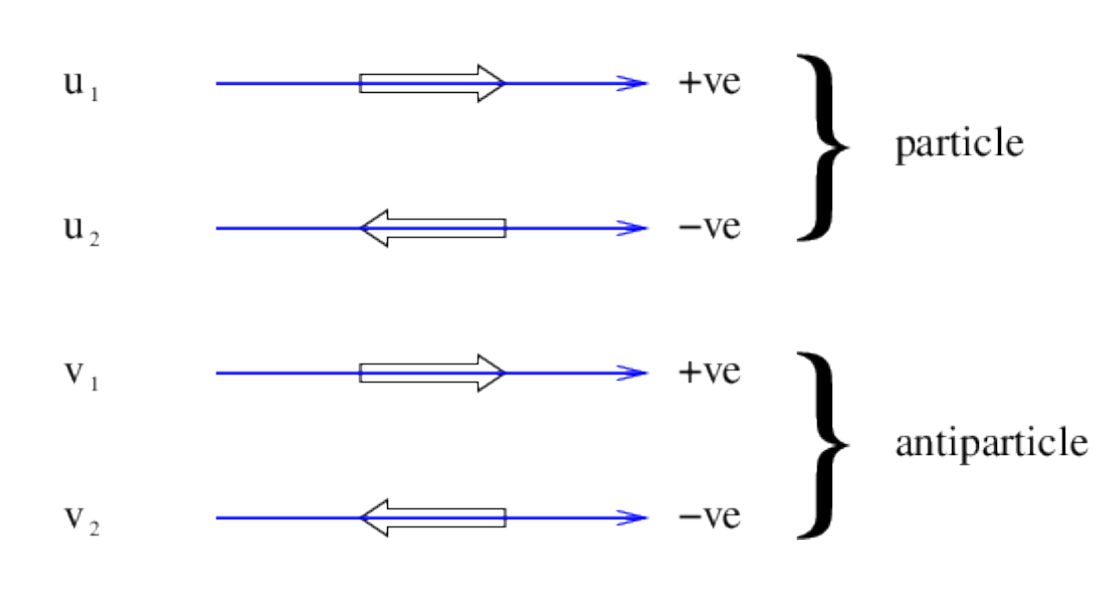
\includegraphics[scale=0.3]{fermions}
\end{figure}

The $u_1, u_2, v_1, v_2$ spinors are only eigenstates of $S_z$ for momentum $\vec{p}$ along the z-axis. There’s nothing special about projecting out the component of spin along the $z$-axis,
that's just the conventional choice. For our purposes it makes more sense to project the spin along the particle’s direction of flight, this defines the \textbf{helicity}, $h$ of the particle.
\begin{align}
\boxed{\hat{h} = \f{\vec{S} \cdot \vec{p}}{\abs{\vec{S}}\abs{\vec{p}}} = \f{2 \vec{S}\cdot\vec{p}}{\abs{\vec{p}}}}
\end{align}
For a spin-1/2 fermion, the two possible values of $h$ are $h = +1$ or $h = −1$. We call $h = +1$ \textbf{right-handed} and $h = −1$ \textbf{left-handed}. Massless fermions, are purely left-handed (only $u_2$); massless antifermions are purely right handed (only $v_1$).













\subsubsection{Probability \& Currents}

Just to be absolutely clear, the metric tensor we are using here is
\begin{align}
\eta_{\mu\nu} = \eta^{\mu\nu} = \begin{pmatrix}
1 &&& \\
&-1&&\\
&&-1&\\
&&&-1
\end{pmatrix}.
\end{align}


 
 
 

\subsubsection{Fermion currents}



To define a Lorentz-invariant quantity to describe fermion currents for QED, we define the \textbf{adjoint spinor}
\begin{align}
\boxed{\bar{\psi} \equiv \psi^\dagger \gamma^0}
\end{align}
where $\psi^\dagger$ is the hermitian conjugate of $\psi$, i.e.,
\begin{align}
\psi = (\psi_1,\psi_2,\psi_3,\psi_4)^\top \implies \psi^\dagger = (\psi_1^*, \psi_2^*, \psi_3^*,\psi_4^*).
\end{align}
With this we have
\begin{align}
\boxed{\bar{\psi} \equiv \psi^\dagger \gamma^0 = (\psi_1^*,\psi_2^*, -\psi_3^*, -\psi_4^*)}
\end{align}
where recall that
\begin{align}
\gamma^0 = \begin{pmatrix}
\mathbb{I} & 0 \\ 0 & \mathbb{I}
\end{pmatrix}.
\end{align}

In order to understand the probability density and probability flow we will want to derive an equation of continuity for the probability. This requires us write down the Dirac equation for $\psi^\dagger$, or equivalently $\bar{\psi}$. The first step is to write the Dirac equation out longhand:
\begin{align}
i\gamma^0 \p_t \psi + i\gamma^1 \p_x \psi + i\gamma^2 \p_y\psi + i\gamma^3 \p_z \psi - m\psi = 0. 
\end{align}
Next, take the hermitian conjugate of this equation:
\begin{align}
\lb i\gamma^0 \p_t \psi + i\gamma^1 \p_x \psi + i\gamma^2 \p_y\psi + i\gamma^3 \p_z \psi - m\psi = 0\rb^\dagger
\end{align}
We have look at the form of each of Dirac's gamma matrices to take the correct hermitian conjugates, which turn out to be:
\begin{align}
{\gamma^\mu}^\dagger
=
\begin{cases}
\gamma^\mu \hspace{0.5cm} \mu = 0\\
-\gamma^\mu \hspace{0.5cm} \mu \neq 0.
\end{cases}.
\end{align}
With this we write
\begin{align}
-i (\p_t \psi^\dagger)\gamma^0 - i ( \p_x \psi^\dagger)(-\gamma^1) - i(\p_y\psi^\dagger)(-\gamma^2) - i (\p_z \psi^\dagger)(-\gamma^3) = m\psi^\dagger .
\end{align}
Now, we multiply both sides by $\gamma^0$ to get
\begin{align}
-i (\p_t \psi^\dagger)\gamma^0\gamma^0 - i (\p_x \psi^\dagger)(-\gamma^1)\gamma^0 - i(\p_y\psi^\dagger)(-\gamma^2)\gamma^0 - i (\p_z \psi^\dagger)(-\gamma^3)\gamma^0 = m\psi^\dagger\gamma^0.
\end{align}
But we note that $\gamma^\mu$ are just matrices of constants, which means we can combine them with $\psi^\dagger$ to get $\bar{\psi}$. But in order to do that, we will have to move $\gamma^0$ closer to $\psi^\dagger$. To do this, we use the relation: $\gamma^0 \gamma^j = -\gamma^j \gamma^0$:
\begin{align}
-i (\p_t \bar{\psi})\gamma^0 - i (\p_x \bar{\psi})\gamma^1   -i(\p_y\bar{\psi})\gamma^2 - i (\p_z \bar{\psi})\gamma^3 = m\bar{\psi}.
\end{align} 
But of course we can succinctly write this as what known as the \textit{adjoint Dirac equation}
\begin{align}
\boxed{\bar{\psi}(i\p_\mu \gamma^\mu + m) = 0}
\end{align} 
where $\p_\mu$ acts on $\bar{\psi}$ from the right. \\

Okay, so now we have two versions of the Dirac equation:
\begin{align}
\begin{cases}
\bar{\psi}(i\p_\mu \gamma^\mu + m) = 0 \\
(i\p_\mu \gamma^\mu - m)\psi = 0 
\end{cases}
\implies
\begin{cases}
\bar{\psi}(i\p_\mu \gamma^\mu + m)\psi = 0 \\
\bar{\psi}(i\p_\mu \gamma^\mu - m)\psi = 0 
\end{cases}.
\end{align}

Adding them gives us
\begin{align}
\bar{\psi}(\p_\mu \gamma^\mu \psi) + \bar{\psi}(i\p_\mu \gamma^\mu)\psi = 0.
\end{align}
But this is just the product rule, so we get
\begin{align}
\boxed{\p_\mu (\bar{\psi} \gamma^\mu \psi ) = 0}
\end{align}
If we define the \textbf{current} as
\begin{align}
j^\mu \equiv (\rho, \vec{j}) = \bar{\psi} \gamma^\mu \psi 
\end{align}
where $\rho$ is the probability density and $\vec{j}$ is the probability 3-current, then we have the conservation law:
\begin{align}
\boxed{\p_\mu j^\mu = 0}
\end{align}

 
This is just the covariant form for an equation of continuity. The probability density is 
\begin{align}
\boxed{\rho = \bar{\psi}\gamma^0\psi = \psi^\dagger {\gamma^0}^2 \psi = \psi^\dagger\psi}
\end{align}
and the probability 3-current $\vec{j}$ is 
\begin{align}
\boxed{\vec{j} = \gamma^\dagger (\gamma^0\gamma^\mu)\psi}
\end{align}


This current is the same one which appears in Feynman diagrams. It is called a vector current, and is the current responsible for the electromagnetic interaction. 






\subsubsection{Maxwell's Equations}



The photon is described by Maxwell's equations. For EM interactions, Maxwell's equations can be written covariant form as
\begin{align}
\boxed{\square A^\mu = 4\pi j^\mu \hspace{0.5cm} \p_\mu A^\mu = 0 \hspace{0.5cm} \p_\mu j^\mu = 0}
\end{align}
The plane wave solution can be written as
\begin{align}
A^\mu = \epsilon^\mu(s) e^{-ip\cdot x} 
\end{align}
where $\epsilon^\mu(s)$ is of course the polarization vector, which depends on the spin $s$ of the photon. 







































\subsubsection{QED rules}



\begin{figure}[!htb]
	\centering
	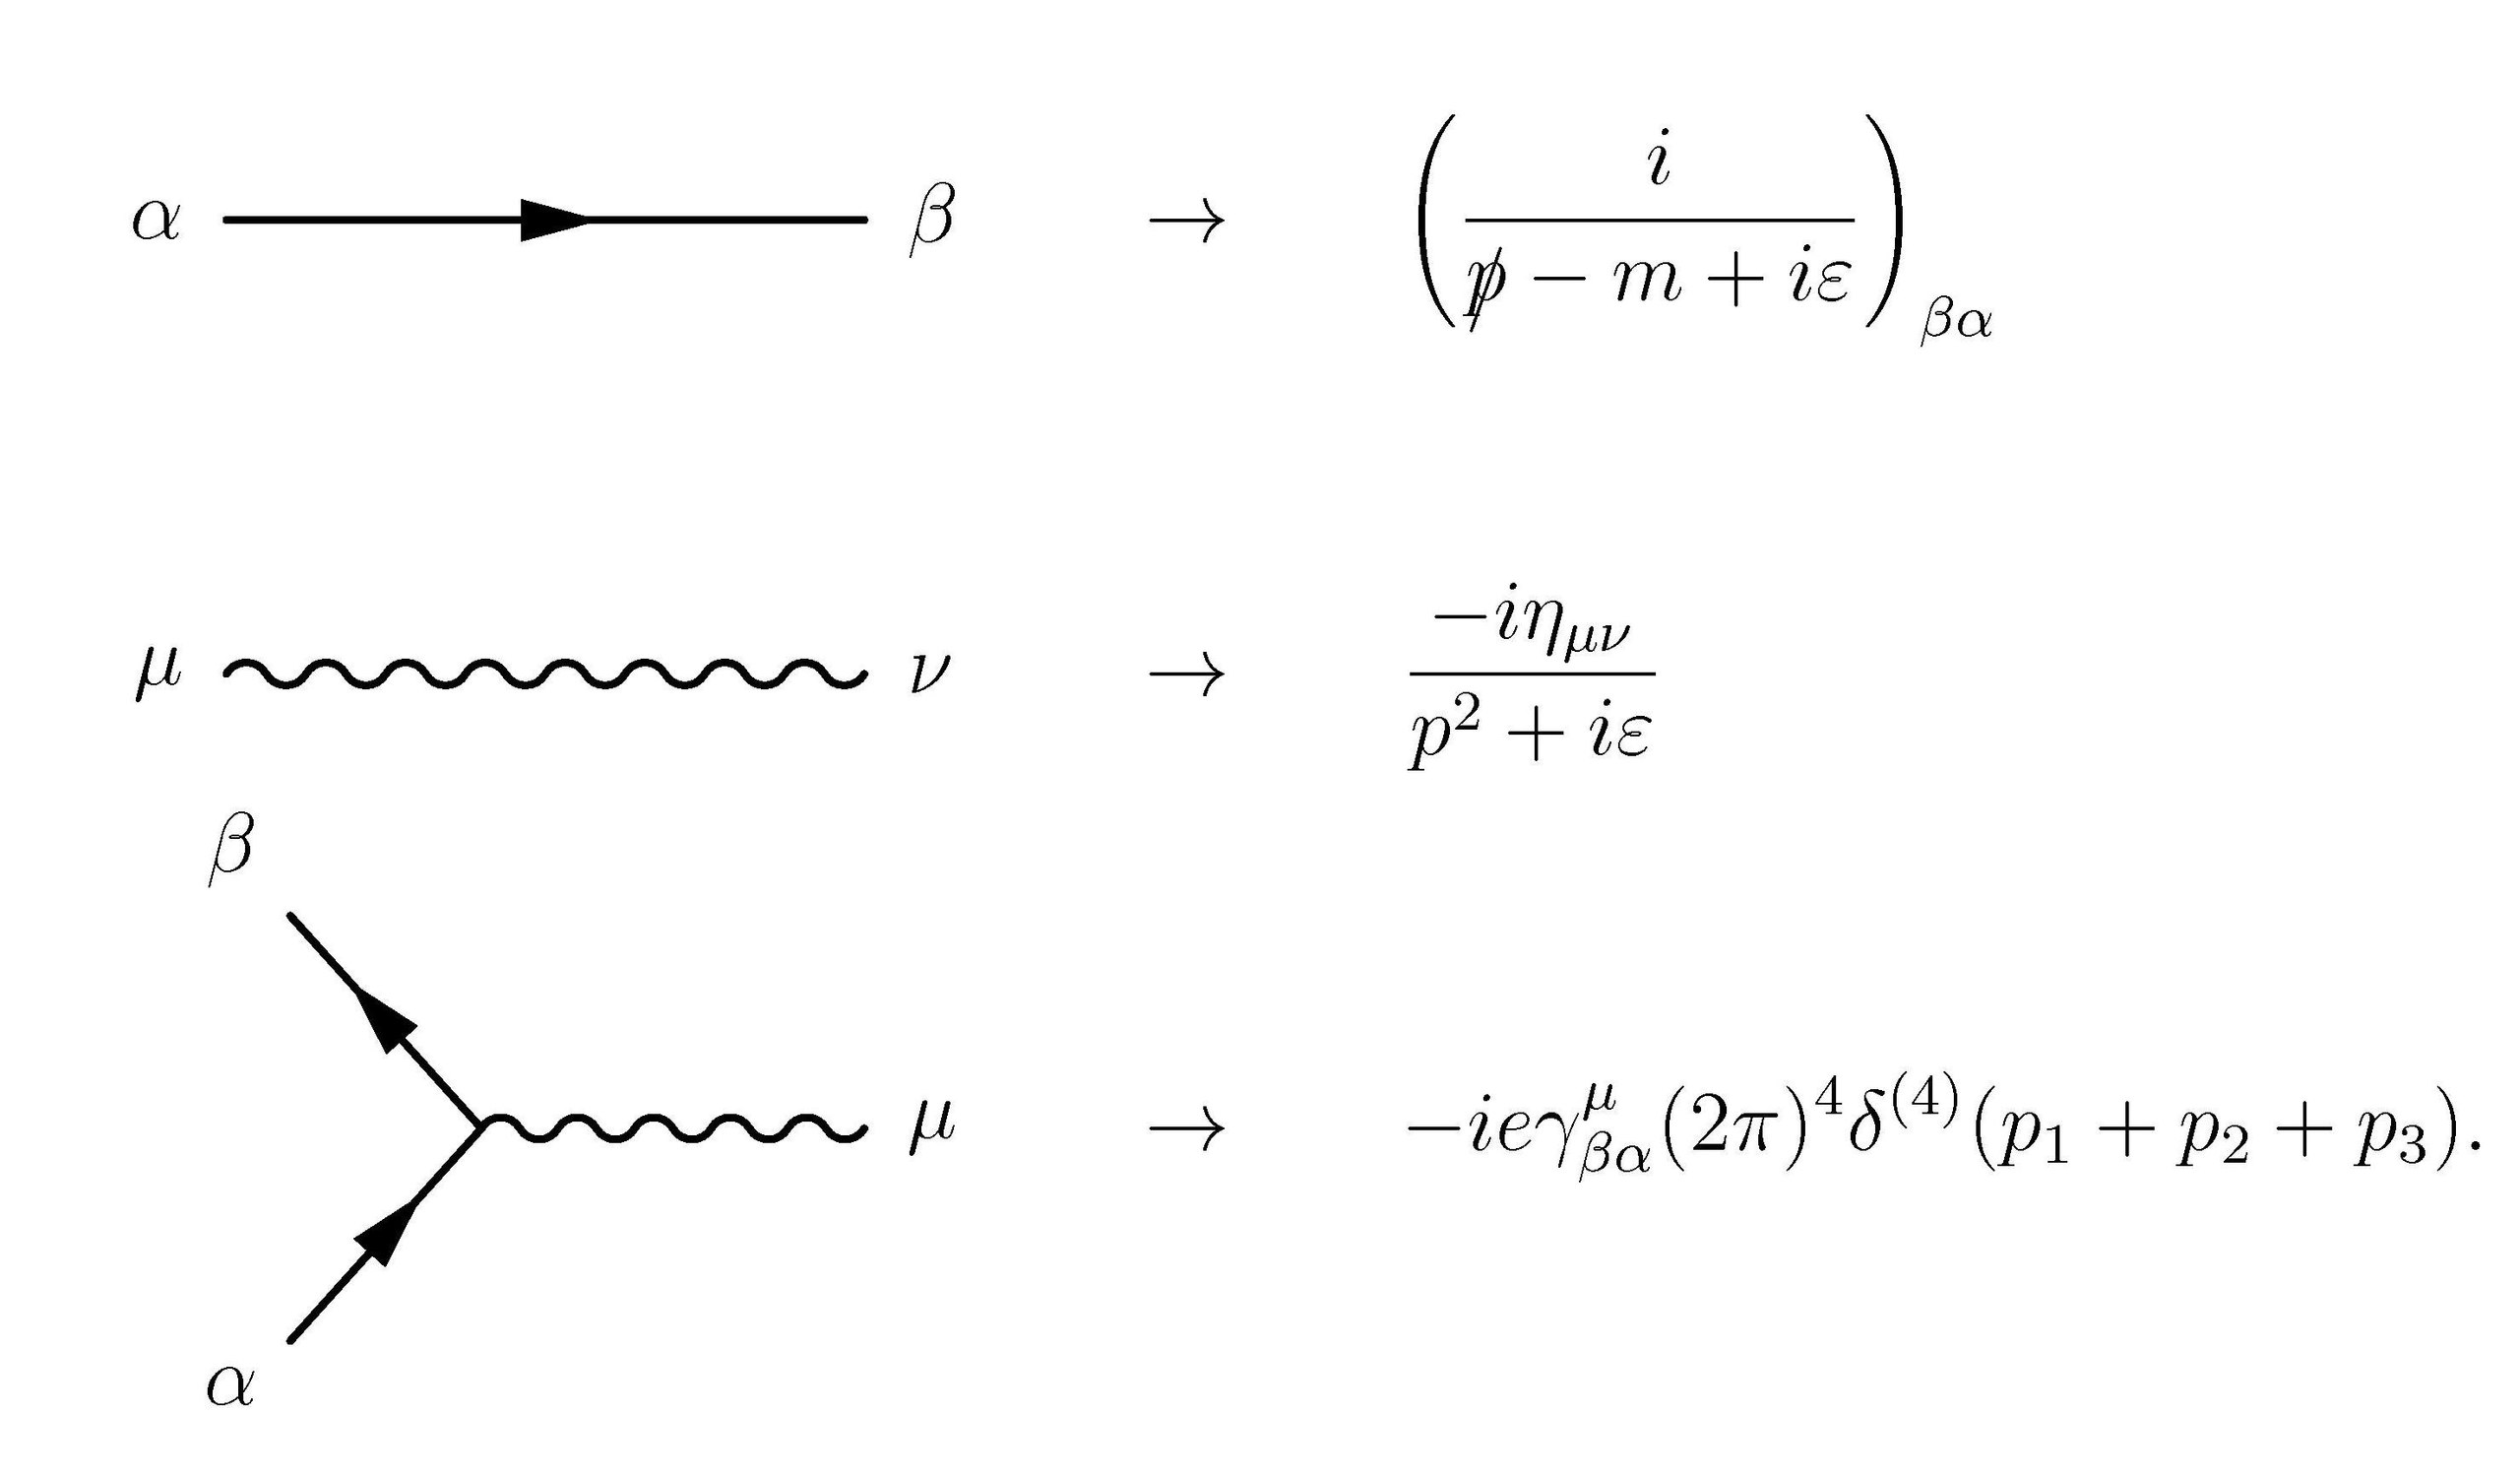
\includegraphics[scale=0.1]{QED}
	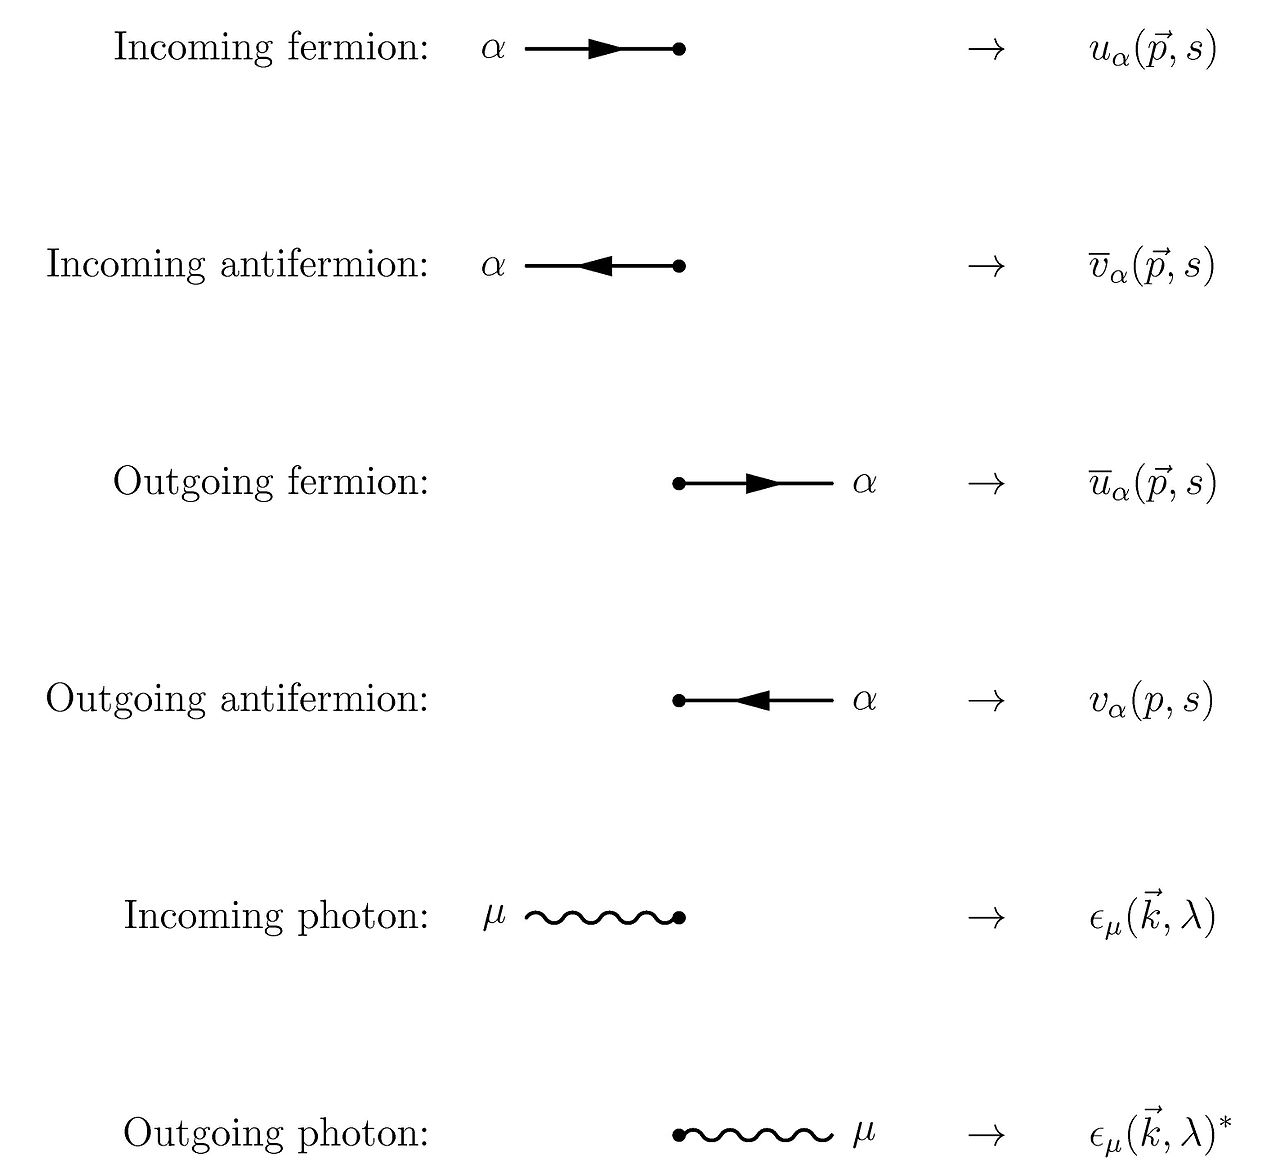
\includegraphics[scale=2]{QED-1}
	\caption{From Wikipedia}
\end{figure}











\newpage


\subsection{The Dirac Equation}


\subsubsection{History}
\subsubsection{Clifford Algebra}
\subsubsection{Cousins of the gamma matrices}
\subsubsection{Lorentz transformation}
\subsubsection{Dirac bilinears}
\subsubsection{Parity}
\subsubsection{The Dirac Lagrangian}
\subsubsection{Slow \& Fast electrons}
\subsubsection{Chirality \& Handedness}
\subsubsection{Interactions}
\subsubsection{Charge conjugation \& antimatter}
\subsubsection{CPT theorem}




\newpage


\subsection{Quantizing the Dirac Field}


\subsubsection{Anticommutation}
\subsubsection{The Dirac field}
\subsubsection{Energy of the vacuum}
\subsubsection{Fermion propagator}


\newpage

\subsection{Lorentz Group \& Weyl Spinors}

\subsubsection{Lorentz algebra}
\subsubsection{From algebra to representation}
\subsubsection{Spinor representations}
\subsubsection{The Dirac equation}


\newpage


\subsection{Spin-statistics connection}



\newpage



\subsection{Vacuum Energy, Grassmann Integrals, \& Feynman Diagrams for Fermions}

\subsubsection{Fermions are weird}
\subsubsection{Vacuum energy}
\subsubsection{A peculiar sign for fermions}
\subsubsection{Grassmann Math}
\subsubsection{Grassmann Path Integrals}
\subsubsection{Dirac propagator}
\subsubsection{Feynman rules for fermions}

\newpage

\subsection{Electron Scattering \& Gauge Invariance}

\subsubsection{Electron-proton scattering}
\subsubsection{Potential scattering}
\subsubsection{Electron-electron scattering}

\newpage


\subsection{Diagrammatic Proof of Gauge Invariance}


\subsubsection{Gauge invariance}
\subsubsection{A specific example}
\subsubsection{Photon landing on an internal line}
\subsubsection{Ward-Takahashi identity}
\subsubsection{The longitudinal mode}
\subsubsection{Emission and absorption of photons
}



\newpage

\subsection{Photon-Electron Scattering and Crossing}

\subsubsection{Photon scattering on an electron}
\subsubsection{Electron-positron annihilation}
\subsubsection{Crossing}
\subsubsection{Special relativity and quantum mechanics require antimatter}



























\newpage



















\section{Renormalization \& Gauge Invariance}




\subsection{Cutoffs}







\subsubsection{Field theory blowing up}

Recall the scattering amplitude (or the Green's function) for a $\lambda^2$ loop diagram is given by:
\begin{align}
\mathcal{M} = \f{1}{2}(-i\lambda)^2\int \f{d^4k}{(2\pi)^4}\f{i}{k^2 - m^2 + i\epsilon}\f{i}{(k_1 + k_2 - k)^2 - m^2 + i\epsilon}.
\end{align}
The associated Feynman diagram is
\begin{figure}[!htb]
	\centering
	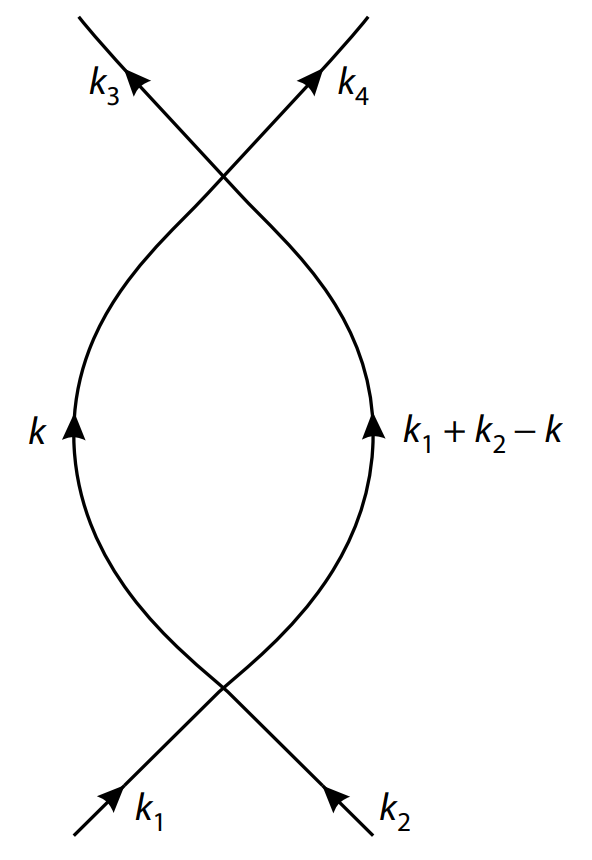
\includegraphics[scale=0.3]{loop-feynman}
	\caption{From Zee}
\end{figure}

We have mentioned in \textit{Loops and a first look at divergence} that this integral diverges when all momentum modes are considered. How do we deal with this? First, let $K \equiv k_1 + k_2$ denote the total initial momentum. We can rewrite the scattering amplitude as
\begin{align}
\mathcal{M} = \f{1}{2}(-i\lambda)^2\int \f{d^4k}{(2\pi)^4}\f{i}{k^2 - m^2 + i\epsilon}\f{i}{(K - k)^2 - m^2 + i\epsilon}.
\end{align} 

We say that this integral diverges \textit{logarithmically} as $\int d^4k/k^4$ for large $k$. We also call this ``ultraviolet divergence'' since the integral diverges when $k$ is large. \\

To deal with this integral, we have to look at ``regularization'' and ``renormalization.'' \textbf{Regularization} is the process of making divergent integrals converge by integrating up to a cutoff $\Lambda$. Physically, this means that whatever quantum field theory we're working with is an effective low energy theory that is valid up to some energy associated with $\Lambda$.  $\Lambda$ should be thought of as physical, ``parameterizing our threshold of ignorance.'' When we evaluate integrals with a cutoff $\Lambda$, we literally integrate only up to $\Lambda$. If the integral is convergent, we say it is ``regularized.'' So what is
\begin{align}
\mathcal{M} = \f{1}{2}(-i\lambda)^2\int^\Lambda \f{d^4k}{(2\pi)^4}\f{i}{k^2 - m^2 + i\epsilon}\f{i}{(K - k)^2 - m^2 + i\epsilon}?
\end{align}
We might be tempted to evaluate this integral directly by the Cauchy integral formula and the residue theorem. But notice that we are not allowed to do that here because we are integrating over 4-dimensional Minkowskian spacetime. We will learn how to actually do this in the following sections.


\subsubsection{Evaluating Feynman diagrams - Zee's Appendix D}

Before trying to evaluating the integral from the previous section, we will first try to evaluate the following integral:
\begin{align}
\boxed{I = \int \f{d^4k}{(2\pi)^4} \f{1}{(k^2 - c^2+ i\epsilon)^3} = \int \f{d^3k}{(2\pi)^3}\int \f{dk_0}{2\pi} \f{1}{(k_0^2 - (\vec{k}^2 + c^2)+ i\epsilon)^3}} 
\end{align}
where we have used the fact that
\begin{align}
k^2 = k_0^2 - \vec{k}^2
\end{align}
based on the Minkowskian metric. \\

Focusing first on the $k_0$ integral, we observe that if we can somehow turn the denominator into the form:
\begin{align}
k_0^2 - (\vec{k}^2 + c^2) + i\epsilon \to k'^2 + c^2 + i\epsilon
\end{align}
then we no longer have to worry about poles. Whether we can do this depends on whether we can somehow flip the sign of $k_0$ from a plus to a minus to agree with the spatial part of $k$. It turns out this is possible, with a slight change of variables and tricks. Define $k_4$ such that
\begin{align}
k_0 = ik_4.
\end{align}
Then 
\begin{align}
dk_0 = idk_4; \hspace{0.5cm} k_0^2 = -k_4^2.
\end{align}
Next, instead of integrating over the real line and close the contour with the northern semi-contour (or southern semi-contour), we can rotate the contour such that we are integrating over the imaginary line and closing the contour using the east/west contour: 
\begin{figure}[!htb]
	\centering
	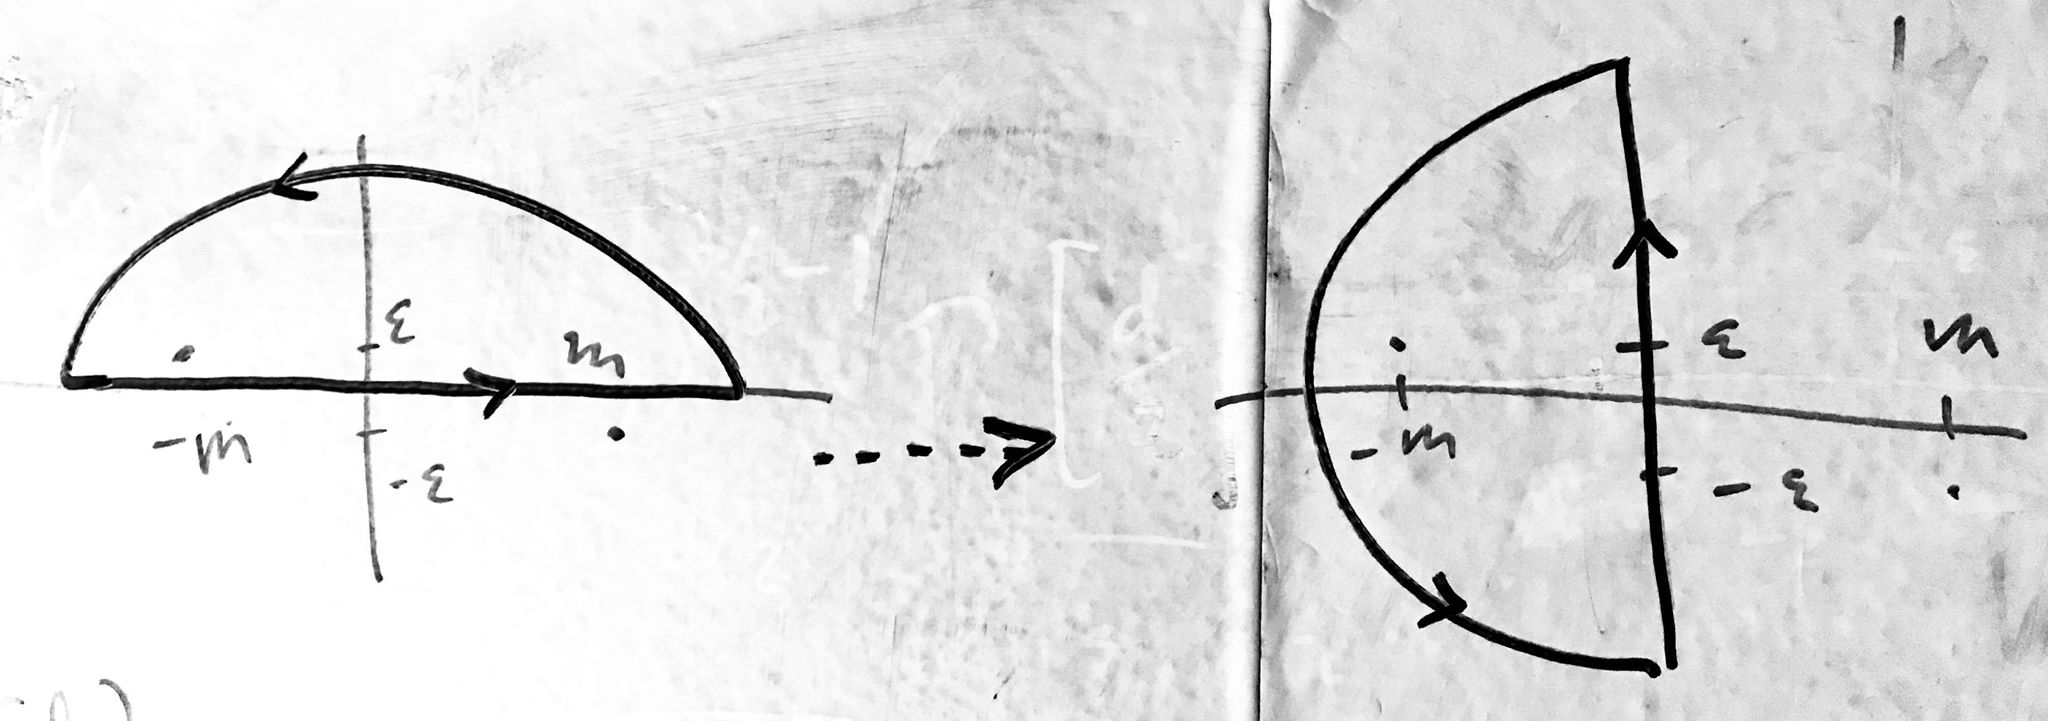
\includegraphics[scale=0.1]{rotate}
\end{figure}

This means
\begin{align}
\int^\infty_{-\infty} dk_0 \f{1}{(k_0^2 - (\vec{k}^2 + c^2)+ i\epsilon)^3} &= \int^{i\infty}_{-i\infty}\f{1}{(k_0^2 - (\vec{k}^2 + c^2)+ i\epsilon)^3} \nonumber\\
&= \int^{-\infty}_{\infty}idk_4\f{1}{(-k_4^2 - (\vec{k}^2 + c^2)+ i\epsilon)^3} \nonumber\\
&= \int^{\infty}_{-\infty}idk_4\f{1}{(\underbrace{k_4^2 + \vec{k}^2} + c^2)^3}; \hspace{0.2cm}\epsilon\to 0 \nonumber\\
&= \int^{\infty}_{-\infty}idk_4\f{1}{(k^2_E + c^2)^3}
\end{align}
where 
\begin{align}
k^2_E = k_4^2 + \vec{k}^2
\end{align}
is the norm square of the Euclidean 4-vector (rather than Minkowskian). With this, we can replace the integration measure
\begin{align}
d^4k \to d^4_Ek
\end{align}
where $d^E k$ is the integration measure in Euclidean 4-dimensional space. So,
\begin{align}
\boxed{I = i(-1)^3\int \f{d^4_E k}{(2\pi)^4} \f{1}{(k^2_E + c^2)^3}}
\end{align}
Good, but how do we evaluate this integral? It is not obvious how we could get integrate out all the angular elements. It turns out that it is more useful for us to look at a more general case where we evaluate
\begin{align}
H = \int d^d_Ek \, F(k^2)
\end{align}
where
\begin{align}
k^2 = k_1^2 + k_2^2 + \dots + k^2_d.
\end{align}
We assume that the integral converges. We will also drop the $E$ subscript for convenience. Suppose we integrate over the $(d-1)$ angular variables to get
\begin{align}
H = C(d)\int^\infty_0 dk\,k^{d-1}F(k^2)
\end{align}
where our $k$ can be thought of as only the radial component. What is $C(d)$? Well, we know that
\begin{align}
J = \int d^dk\, e^{-k^2/2} = \lp\sqrt{2\pi}\rp^d,
\end{align}
from our results in \textit{Gaussian integrals and their moments}. But we also know that alternatively,
\begin{align}
J &= \int d^dk\, e^{-k^2/2}\nonumber\\
&= C(d) \int^\infty_0 dk\, k^{d-1}e^{-k^2/2} \hspace{0.5cm}\text{angular-integrated} \nonumber\\
&= C(d) 2^{d/2 - 1} \int^\infty_0 dx\, x^{d/2 - 1}e^{-x} \nonumber\\
&= C(d) 2^{d/2 - 1} \Gamma\lp \f{d}{2} \rp
\end{align}
where we have made the necessary change of variables in order to the get the integral representation of the Gamma function, which shows up quite often in probability theory:
\begin{align}
{\Gamma(z) = \int^\infty_0 x^{z-1}e^{-x}\,dx, \hspace{0.5cm} \Re(z) > 0}
\end{align}
which satisfies the definition of the Gamma function defined for positive integers:
\begin{align}
\Gamma(n) = (n-1)! \iff \Gamma(n+1) = n\Gamma(n),
\end{align}
which we can show by integration by parts. It follows that
\begin{align}
\lp 2\pi \rp^{d/2} = C(d) 2^{d/2 - 1} \Gamma\lp \f{d}{2} \rp,
\end{align}
which means 
\begin{align}
\boxed{C(d) = \f{2\pi^{d/2}}{\Gamma\lp d/2 \rp}}
\end{align}
As a little ``sanity check,'' when $d=2$, when $C(d) = 2\pi$. When $d=3$, $C(d) = 4\pi$, which are familiar angular elements in 2 and 3 dimensions. With this, we have in general,
\begin{align}
\boxed{H = \int d^d_E k \,F(k^2) = C(d)\int^\infty_0 dk\, k^{d-1}F(k^2)= \f{2\pi^{d/2}}{\Gamma\lp d/2 \rp}\int^\infty_0 dk\, k^{d-1}F(k^2)}
\end{align}

So, when $d=4$ (which \textbf{is the }value of $d$ we are interested in), 
\begin{align}
\int d^4_E k \, F(k^2) = (2\pi^2) \int^\infty_0 dk\,k^3 F(k^2).
\end{align}
With this, we can now evaluate the original $I$:
\begin{align}
I &= \int \f{d^4k}{(2\pi)^4} \f{1}{(k^2 - c^2+ i\epsilon)^3}\nonumber\\
&= \dots \nonumber\\ 
&= i(-1)^3\int \f{d^4_E k}{(2\pi)^4} \f{1}{(k^2_E + c^2)^3} \nonumber\\
&= \f{-i}{(2\pi)^4}\int d^4_E k k^3 \f{1}{(k^2 + c^2)^3}  \nonumber\\
&= \f{-i}{(2\pi)^4} (2\pi^2) \underbrace{\int^\infty_0 dk\,k^3   \f{1}{(k^2 + c^2)^3}} \nonumber\\
&= \f{-i}{(2\pi)^4} (2\pi^2) \f{1}{4c^2} \nonumber\\
&= {\f{-i}{32 \pi^2 c^2}},
\end{align}
where the final integral can be evaluated in Mathematica as follows:
\begin{lstlisting}
In[9]:= Integrate[k^3/(k^2 + c^2)^3, {k, 0, Infinity}]

Out[9]= ConditionalExpression[1/(4 c^2), Re[c] != 0]
\end{lstlisting}
$\,$\\

Thus, we have derived the basic formula for doing Feynman integrals:
\begin{align}
\boxed{\int \f{d^4k}{(2\pi)^4} \f{1}{(k^2 - m^2+ i\epsilon)^3} = \f{-i}{32 \pi^2 m^2}}
\end{align}
Okay, what if now we only integrate to a cutoff $\Lambda$ and with a power of $2$ (not $3$) in the denominator, i.e.,
\begin{align}
\int^{k=\Lambda} \f{d^4k}{(2\pi)^4} \f{1}{(k^2 - m^2+ i\epsilon)^2} = ?
\end{align}
Essentially, we can work through the same steps again. Notice that the cutoff is only in $k$ but not in the angular pieces, so we still have that
\begin{align}
\int^{k=\Lambda} \f{d^4k}{(2\pi)^4} \f{1}{(k^2 - m^2+ i\epsilon)^2} &= \f{-i}{(2\pi)^4}(2\pi^2)\int^{k=\Lambda} dk\,k^3\f{1}{(k^2 + m^2)^2}\nonumber\\
&= \f{-i}{8\pi^2}\int^{k=\Lambda} dk\,k^3\f{1}{(k^2 + m^2)^2}
\end{align}
This last integral can be evaluated in Mathematica as follows:
\begin{lstlisting}
In: Integrate[k^3/(k^2 + a^2)^2, {k, 0, L}]

Out: 1/2(-1-Log[a^2])+(a^2+(a^2+L^2)Log[a^2+L^2])/(2(a^2+L^2)) 
\end{lstlisting}

Technical side note: In reality Mathematica gives a bunch of conditional statements, but we can just ignore those since we're only working with real momenta here. \\

So, we have
\begin{align}
\int^{\Lambda} \f{d^4k}{(2\pi)^4} \f{1}{(k^2 - m^2+ i\epsilon)^2} &= \f{-i}{16\pi^2}\lc -1 - \log(m^2) + \log(m^2 + \Lambda^2) + \f{m^2 }{m^2 + \Lambda^2} \rc\nonumber\\
&= \f{-i}{16\pi^2}\lc -1  + \log\lp\f{ m^2 + \Lambda^2}{m^2} \rp+ \f{m^2 }{m^2 + \Lambda^2} \rc.
\end{align}

Assuming $\lambda^2 \gg m^2$, we have that
\begin{align}\label{Feynman-int}
\boxed{\int^{\Lambda} \f{d^4k}{(2\pi)^4} \f{1}{(k^2 - m^2+ i\epsilon)^2} \approx \f{i}{16\pi^2} \lb \log\lp \f{\Lambda^2}{m^2} \rp  - 1 + \dots \rb}
\end{align}




As an exercise, let's try to evaluate
\begin{align}
\int^{\Lambda} \f{d^4k}{(2\pi)^4} \f{k^2}{(k^2 - m^2+ i\epsilon)^2}.
\end{align}
Well, most things are similar except for the  form of $F(k^2)$. So we have
\begin{align}
\int^{k=\Lambda} \f{d^4k}{(2\pi)^4} \f{k^2}{(k^2 - m^2+ i\epsilon)^2} &= \f{-i}{(2\pi)^4}(2\pi^2)\int^{k=\Lambda} dk\,k^3\f{k^2}{(k^2 + m^2)^2}\nonumber\\
&= \f{-i}{8\pi^2}\int^{k=\Lambda} dk\,\f{k^5}{(k^2 + m^2)^2}.
\end{align}
Once again with the help of Mathematica, we find 
\begin{lstlisting}
In: Integrate[k^5/(k^2 + a^2)^2, {k, 0, L}]

Out: ((2a^2 L^2+L^4+2a^2(a^2+L^2)(Log[a^2]-Log[a^2+L^2]))/(2(a^2+L^2)))
\end{lstlisting}
Thus,
\begin{align}
\int^{k=\Lambda} \f{d^4k}{(2\pi)^4} \f{k^2}{(k^2 - m^2+ i\epsilon)^2} &\approx \f{-i}{16\pi^2}\lc m^2 + \Lambda^2 + 2m^2\log\lp \f{m^2}{m^2 + \Lambda^2} \rp  \rc \nonumber\\
&= \f{-i}{16\pi^2}\lc m^2 + \Lambda^2 - 2m^2\log\lp \f{\Lambda^2}{m^2} \rp + \dots  \rc
\end{align}
where once again we assume $\Lambda^2 \gg m^2$. So we have
\begin{align}
\boxed{\int^{k=\Lambda} \f{d^4k}{(2\pi)^4} \f{k^2}{(k^2 - m^2+ i\epsilon)^2} = \f{-i}{16\pi^2}\lc m^2 + \Lambda^2 - 2m^2\log\lp \f{\Lambda^2}{m^2} \rp + \dots  \rc}
\end{align}




\subsubsection{Denominator Combination Identity - Zee's Appendix D}

Now, for general Feynman integrals/diagrams, we don't often have a single term raised to some power in the denominator such as
\begin{align}
\f{1}{(k^2 - m^2 + i\epsilon)^n}.
\end{align}
For loop diagrams where there are multiple inner loops and possible intermediate momenta, we will have things like
\begin{align}
\f{1}{(k_1^2 - m^2 + i\epsilon)^l} \dots \f{1}{(k_n^2 - m^2 + i\epsilon)^p}
\end{align}
and so on. It would be nice if we could somehow split this product into a sum of integrals that we can evaluate. Fortunately, we have a useful identity in combining denominators:
\begin{align}
\boxed{\f{1}{x_1\dots x_n} = (n-1)! \int^1_0\dots \int^1_0 d\alpha_1\dots d\alpha_n \, \delta\lp 1 - \sum^n_{j=1} \alpha_j \rp \f{1}{(\alpha_1 x_1 + \dots + \alpha_n x^n)^n}}
\end{align}
For example, when $n=2$, we have
\begin{align}
\boxed{\f{1}{xy} = \int^1_0 d\alpha \, \f{1}{[\alpha x +(1-\alpha)y]^2}}
\end{align}
For $n=3$, we have
\begin{align}
\boxed{\f{1}{xyz}} &= 2\int^1_0 \int^1_0 \int^1_0 d\alpha d\beta d\gamma\, \delta(\alpha + \beta + \gamma - 1) \f{1}{[\alpha x + \beta y + \gamma z]^3} \nonumber\\
&= \boxed{2\iint_{\text{triangle}} d\alpha d\beta\, \f{1}{[z + \alpha(x-z) + \beta(y -z)]^3}}
\end{align}
where the integration region is the triangle in the $\alpha-\beta$ plane bounded by $0 \leq \beta \leq 1 - \alpha$ and $0 \leq \alpha \leq 1$. \\

These identities will be extremely useful in the following sections.
















\subsubsection{Pauli-Villars regularization}

Now we're getting closer to evaluating $\mathcal{M}$ up to cutoff $\Lambda$. To turn the integrand of
\begin{align}
\mathcal{M} = \f{1}{2}(-i\lambda)^2\int \f{d^4k}{(2\pi)^4}\f{i}{k^2 - m^2 + i\epsilon}\f{i}{(K - k)^2 - m^2 + i\epsilon}.
\end{align}
into something we can integrate over, we first apply the following identity from the previous section
\begin{align}
\f{1}{xy} = \int^1_0 d\alpha \f{1}{[\alpha x + (1-\alpha )y]^2}
\end{align}
with 
\begin{align}
y = k^2 - m^2 + i\epsilon \hspace{1cm} x = (K - k)^2 - m^2 + i\epsilon.
\end{align}
Then we have
\begin{align}
\mathcal{M} = \f{1}{2}(-i\lambda)^2 i^2 \int \f{d^4k}{(2\pi)^4}\int^1_0 d\alpha\, \f{1}{D}
\end{align}
where
\begin{align}
D &=  \dots \nonumber \text{some approximations here}\\
& =[\alpha(K-k)^2 + (1-\alpha)k^2 - m^2 + i\epsilon]^2 \nonumber\\
&= [(k - \alpha K)^2 + \alpha(1-\alpha)K^2- m^2   + i\epsilon]^2 \nonumber \hspace{0.5cm}\text{completing the squares}.
\end{align}

Consider the change of variables (called \textit{Feynman variables})
\begin{align}
\kappa =  k - \alpha K \implies d^4k \to d^4\kappa,
\end{align}
then we get
\begin{align}
D = [\kappa^2 + \alpha(1-\alpha)K^2 - m^2 + i\epsilon]^2 = [\kappa^2 - M_0^2 + i\epsilon ]^2
\end{align}
where
\begin{align}
M_0^2 = m^2  - \alpha(1 - \alpha)K^2.
\end{align}
Thus,
\begin{align}
\mathcal{M} &= \f{1}{2}(-i\lambda)^2 i^2 \int \f{d^4\kappa}{(2\pi)^4} \int^1_0 d\alpha\,\f{1}{D} \nonumber\\
&= \f{1}{2}(-i\lambda)^2 i^2 \int \f{d^4\kappa}{(2\pi)^4}  \int^1_0 d\alpha \, \f{1}{[\kappa^2 - M_0^2 + i\epsilon ]^2}\nonumber\\
&= {\f{1}{2}(-i\lambda)^2 i^2  \int^1_0 d\alpha \int \f{d^4\kappa}{(2\pi)^4}  \, \f{1}{[\kappa^2 - M_0^2 + i\epsilon ]^2}}
\end{align}
Imposing a cutoff, we get
\begin{align}
\boxed{\mathcal{M} = \f{1}{2}(-i\lambda)^2 i^2  \int^1_0 d\alpha \int^\Lambda \f{d^4\kappa}{(2\pi)^4}  \, \f{1}{[\kappa^2 - M_0^2 + i\epsilon ]^2}}
\end{align}

Aha! In integral over $d^4 \kappa$ is something we know how to do. Repeating the steps in the previous sections regarding evaluating Feynman integrals, we first go to Euclidean space, then integrate over all angular components so that we are left with a $d_E k\, k^{3}$ integral. In fact, we have evaluated the $k$ integral. \\


Applying the result from \eqref{Feynman-int} to get
\begin{align}\label{exact}
\mathcal{M} &= \f{1}{2}(-i\lambda)^2 i^2  \int^1_0 d\alpha\int^{\Lambda} \f{d^4\kappa}{(2\pi)^4} \f{1}{(\kappa^2 - M_0^2+ i\epsilon)^2} \nonumber \\
&\approx \f{1}{2}(-i\lambda)^2 i^2  \int^1_0 d\alpha \f{i}{16\pi^2} \lb \log\lp \f{\Lambda^2}{M_0^2} \rp  - 1 + \dots \rb \nonumber\\
&= \f{i\lambda^2}{32\pi^2} \int^1_0 d\alpha\, \lb \log\lp \f{\Lambda^2}{M_0^2} \rp  - 1 + \dots \rb.
\end{align}
We have to keep in mind that $M_0^2(\alpha) = m^2  - \alpha(1 - \alpha)K^2$. For $\Lambda^2 \gg M_0^2$, the log term dominates the square brackets, so we can just ignore the $-1$ term. With this, we have
\begin{align}\label{amplitudeM}
\boxed{\mathcal{M}  = \f{i\lambda^2}{32\pi^2} \int^1_0 d\alpha\,  \log\lp \f{\Lambda^2}{m^2  - \alpha(1 - \alpha)K^2 - i\epsilon} \rp }
\end{align}
Thus we see that the integrand scales logarithmically. \\








Alternatively, \textbf{Pauli-Villars regularization} tells us that we can do the following (justified) substitution:
\begin{align}\label{Pauli-Villars}
\boxed{\int^\Lambda \f{d^4\kappa}{(2\pi)^4}  \, \f{1}{[\kappa^2 - M_0^2 + i\epsilon ]^2} \to \int^\Lambda \f{d^4\kappa}{(2\pi)^4}  \, \lb\f{1}{(\kappa^2 - M_0^2 + i\epsilon )^2} - \f{1}{(\kappa^2 - \Lambda^2 + i\epsilon)^2}\rb}
\end{align}
where $\Lambda^2 \gg M_0^2$. This is a reasonable proposition because for $\Lambda^2$ that is very large this additive term is negligible compared to the first term. \\



We know from the previous section with the Feynman integrals that
\begin{align}\label{feym}
{\int \f{d^4k}{(2\pi)^4} \f{1}{(k^2 - c^2+ i\epsilon)^3} = \f{-i}{32\pi^2 c^2}}
\end{align}


So, if we differentiate \eqref{Pauli-Villars} with respect to $M_0^2$ (so that we get a power of 3 in the denominator), we get
\begin{align}
&\f{\p}{\p M_0^2} \int^\Lambda \f{d^4\kappa}{(2\pi)^4}   \, \lb\f{1}{(\kappa^2 - M_0^2 + i\epsilon )^2} - \f{1}{(\kappa^2 - \Lambda^2 + i\epsilon)^2}\rb \nonumber\\
= &\int^\Lambda \f{d^4\kappa}{(2\pi)^4}   \, \f{2}{(\kappa^2 - M_0^2 + i\epsilon )^3} \nonumber\\
= &\f{-i}{16\pi^2 M_0^2} \hspace{0.5cm} \text{according to \eqref{feym}}. 
\end{align}

Thus, by reintegrating we get
\begin{align}
\int^\Lambda \f{d^4\kappa}{(2\pi)^4}   \, \lb\f{1}{(\kappa^2 - M_0^2 + i\epsilon )^2} - \f{1}{(\kappa^2 - \Lambda^2 + i\epsilon)^2}\rb = \f{-i}{16\pi^2}\log\lp M_0^2\rp + C.
\end{align}

Repeating this process, but starting with differentiating with respect to $\Lambda^2$ then reintegrating, we get
\begin{align}
\int^\Lambda \f{d^4\kappa}{(2\pi)^4}   \, \lb\f{1}{(\kappa^2 - M_0^2 + i\epsilon )^2} - \f{1}{(\kappa^2 - \Lambda^2 + i\epsilon)^2}\rb = \f{i}{16\pi^2}\log\lp \Lambda^2\rp + \tilde{C}.
\end{align}
This is true when
\begin{align}
C = \f{i}{16\pi^2}\log\lp \Lambda^2\rp \hspace{0.5cm}\text{and}\hspace{0.5cm} \tilde{C} = \f{-i}{16\pi^2}\log\lp M_0^2\rp.
\end{align}
And therefore, we deduce that
\begin{align}
\boxed{\int^\Lambda \f{d^4\kappa}{(2\pi)^4}   \, \lb\f{1}{(\kappa^2 - M_0^2 + i\epsilon )^2} - \f{1}{(\kappa^2 - \Lambda^2 + i\epsilon)^2}\rb = \f{i}{16\pi^2}\log\lp \f{\Lambda^2}{M_0^2} \rp}
\end{align}
So, the scattering amplitude is
\begin{align}
\boxed{\mathcal{M} = \f{i\lambda^2}{32\pi^2}\int^1_0 d\alpha\, \log\lp \f{\Lambda^2}{M_0(\alpha)^2} \rp }
\end{align}

This matches up exactly with what we found in Eq. \eqref{amplitudeM}, where again $M_0(\alpha) = m^2- \alpha(1-\alpha)K^2$.












\subsubsection{Evaluating $\mathcal{M}$ - my attempt}

From \eqref{exact}, we have roughly
\begin{align}
\mathcal{M}  = \f{i\lambda^2}{32\pi^2} \int^1_0 d\alpha\,\lb -1 + \log\lp \f{\Lambda^2}{m^2  - \alpha(1 - \alpha)K^2 - i\epsilon} \rp \rb,
\end{align}
in the $m^2 \ll K^2 \ll \Lambda^2$ limit, we can just set $m^2 = 0$ and actually evaluate this integral in Mathematica to find
\begin{align}
\boxed{\mathcal{M} = \f{i\lambda^2}{32\pi^2} \lb 1 + \log\lp \f{\Lambda^2}{-K^2}\rp \rb}
\end{align}
Here's the Mathematica code:
\begin{lstlisting}
In[37]:= Integrate[Log[L^2/(-a (1 - a) K^2) ] - 1, {a, 0, 1}]

Out[37]= 1 + Log[-(L^2/K^2)]
\end{lstlisting}


Now this is \textbf{not} what Zee got, and I can't seem to see why. But \href{http://sites.krieger.jhu.edu/jared-kaplan/files/2016/05/QFTNotes.pdf}{\underline{this}} source from Johns Hopkins, page 113/260, confirms my answer.  
















\subsubsection{Parameterizing $M_0$ - (Zee way)}

We have seen that the expression for the scattering amplitude after Pauli-Villars regularization is
\begin{align}
\mathcal{M}  = \f{i\lambda^2}{32\pi^2} \int^1_0 d\alpha\,  \log\lp \f{\Lambda^2}{m^2  - \alpha(1 - \alpha)K^2 - i\epsilon} \rp 
\end{align}
For simplicity let's just assume that $m^2 \ll K^2$, so that we can ignore the $m^2$ term in the integrand when necessary. \\


From here, I'll just take Zee's words for it. Essentially, this leftover is not an easy integral to evaluate without assuming $m^2 \to 0$. Zee says that this one-loop $\phi^4$ amplitude comes out to be
\begin{align}
\boxed{\mathcal{M} = 2i\lambda^2C \log \lp \f{\Lambda^2}{K^2} \rp}
\end{align}
where $C$ is some numerical constant. At this point, we use kinematics variables
\begin{align}
s &\equiv K^2 = (k_1 + k_2)^2\\
t &\equiv (k_1 - k_3)^2\\
u &\equiv (k_1 - k_4)^2
\end{align}
whose relations are given in II.6 in Zee's book. It turns out that we can write the scattering amplitude for meson-meson scattering (which includes both a tree and a loop) as
\begin{align}
\boxed{\mathcal{M}_{\text{meson}} = -i\lambda + iC\lambda^2\lb  \log\lp \f{\Lambda^2}{s} \rp + \log\lp \f{\Lambda^2}{t} \rp + \log\lp \f{\Lambda^2}{u} \rp \rb + \dots}
\end{align}
This says after regularization, we speak of cutoff-dependent quantities instead of divergent quantities, and $\mathcal{M}$ depends logarithmically on the cutoff (or more precise the square of it).



















\subsubsection{What is actually measured}



Suppose experiments measure a scattering amplitude of $i\lambda_P$. By the our calculation, it has to be true that
\begin{align}
-i\lambda_P = -i\lambda + iC\lambda^2\lb  \log\lp \f{\Lambda^2}{s} \rp + \log\lp \f{\Lambda^2}{t} \rp + \log\lp \f{\Lambda^2}{u} \rp \rb + \dots.
\end{align}

Calling the sum of the logarithms in the square brackets $L$, we can write
\begin{align}
\mathcal{M} = -i\lambda_P = -i\lambda + iC\lambda^2 L + \dots.
\end{align}
Let
\begin{align}
-i\lambda_P = -i\lambda + iC\lambda^2 L_0
\end{align}
where
\begin{align}
L_0 \equiv \lb    \log\lp \f{\Lambda^2}{s_0} \rp + \log\lp \f{\Lambda^2}{t_0} \rp + \log\lp \f{\Lambda^2}{u_0} \rp \rb
\end{align}
This gives the relationship between $\lambda_P$ and $\lambda$. With this, we can solve for $\lambda$ in terms of $\lambda_P$:
\begin{align}
-i\lambda = -i\lambda_P - iC\lambda^2 L_0 + \mathcal{O}(\lambda^3) = -i\lambda_P - iC\lambda^2_P L_0 + \mathcal{O}(\lambda_P^3).
\end{align}
So we have
\begin{align}
\mathcal{M} = -i\lambda_P - iC\lambda_P^2 L_0 +iC\lambda_P^2 L + \mathcal{O}(\lambda_P^3).
\end{align}


Now, we see that in the scattering amplitude of $\mathcal{M}$ there is a combination of
\begin{align}
L - L_0 = \log \lp \f{s_0}{s} \rp + \log \lp \f{t_0}{t} \rp + \log \lp \f{u_0}{u} \rp,
\end{align}
i.e.,
\begin{align}
\boxed{\mathcal{M} = -i\lambda_P + iC\lambda_P^2 \lb \log \lp \f{s_0}{s} \rp + \log \lp \f{t_0}{t} \rp + \log \lp \f{u_0}{u} \rp  \rb + \mathcal{O}(\lambda_P^3)}
\end{align}


This tells us that when the scattering amplitude is expressed in terms of the physical coupling constant $\lambda_P$, the cut off $\Lambda$ disappears. \\


And so the take-away point here is that we should express physical quantities not in terms of fictitious quantities such as $\lambda$, but in terms of physical, measurable quantities such as $\lambda_P$. \\

The quantity $\lambda_P$ is often referred to as the ``renormalization coupling constant,'' or ``physical coupling constant'' in Zee's words.  















\newpage

\subsection{Renormalizable vs. Nonrenormalizable}



It turns out that there are theories that are ``renormalizable,'' which means scattering amplitudes can be written in terms of physical quantities with no dependence on cutoffs (at least to some orders of $\lambda_P^2$). There are, however, theories in which this cannot happen. These are called ``nonrenormalizable theories.''\\

Einstein's theory of gravity is an example of a nonrenormalizable theory. 


\subsubsection{Dimensional Analysis as Test}


It also turns out that by looking at dimensions of particular terms we can tell if a theory is renormalizable or not. \\

First, we have 
\begin{align}
\hbar = c = 1.
\end{align}
This says length and time has the same dimension, which is the inverse of the dimension of mass. \\

The action has the form
\begin{align}
S \equiv \int d^4x\,\lag
\end{align}
which appears in the path integral as
\begin{align}
e^{iS}
\end{align}
so both the path integral and the action have to be dimensionless. Therefore, the Lagrangian density must have dimension of space raised to to the minus 4 power, i.e., the Lagrangian density has dimension as the 4th power of mass. We denote this as
\begin{align}
[\lag] = 4.
\end{align}
And so in this notation 
\begin{align}
[x] &= 1 \\ 
[\p] &= -1.
\end{align}

Based on the scalar field theory
\begin{align}
\lag = \f{1}{2}[(\p\phi)^2 - m^2 \phi^2]  - \lambda \phi^4.
\end{align}
To make $[\lag] = 4$, we must have
\begin{align}
[\phi] = 1
\end{align}
which implies
\begin{align}
[\lambda] = 0.
\end{align}


So, the coupling $\lambda$ is dimensionless. \\


For fermion field $\phi$, the Lagrangian density is
\begin{align}
\lag = \bar{\psi} i \gamma^\mu \p_\mu \psi + \dots
\end{align}
must have dimension 4. But because $[\p] = 1$ and $[\lag] = 4$ and there are two factors of $\psi$, we must have
\begin{align}
[\psi] = \f{3}{2}.
\end{align} 


From the Maxwell Lagrangian density
\begin{align}
\lag = -\f{1}{4}F_{\mu\nu}F^{\mu\nu}.
\end{align}
This has dimension 4 as always, and so the vector potential must have dimension 1, because each $F_{\mu\nu}$ has dimensions of a $\p_\nu A_\mu$. This tells us that
\begin{align}
[A_\mu] = [\phi] = 1,
\end{align}
i.e., vectors fields have the same dimension as scalar fields.



\subsubsection{Scattering amplitudes blowing up}


Suppose we have a theory where the scattering amplitude up to second order is
\begin{align}
\mathcal{M} \sim G + G^2(?)
\end{align}
where
\begin{align}
[G] = -2.
\end{align}
Then the $(?)$ must take dimension $2$. The only possibility for $(?)$ is $\Lambda^2$, since $[\Lambda] = 1$. Cutoffs have units of mass/energy/momentum. Without a cutoff on the theory, $\Lambda = \infty$. An example of this is Fermi's weak interaction theory.



\subsubsection{Einstein's gravity blowing up}


Einstein's GR is nonrenormalizable. Newton's gravitation constant (or should we say the physical coupling constant) has dimension of $-2$. So just as before, a $\Lambda^2$ is needed in writing out the scattering amplitude, but this blows up as $\Lambda \to \infty$ (without a cutoff). 












\newpage

\subsection{Perturbation Theory \& Degree of Divergence}




\subsubsection{Renormalizability}


From the last section, we see that theories whose coupling constant $\lambda, G,$ etc have negative (mass) dimensions are \textbf{nonrenormalizable}. QED and the $\phi^4$ theory which have the dimensionless coupling constant are renormalizable. However, it is difficult to prove in general that a given theory is renormalizable. It is often easier to prove that a theory is nonrenormalizable. \\


Let's revisit the $\phi^4$ theory. We know that the scattering amplitude has some form (correct as far as dimensions are concerned) of
\begin{align}
-i\lambda_P = -i\lambda + 3iC \log \lp \f{\Lambda^2}{\mu^2} \rp + \mathcal{O}(\lambda^3).
\end{align}


We saw that to order $\lambda^2$ the meson-meson scattering amplitude when expressed in terms of the physical coupling constant is independent of the cutoff $\Lambda$. But how can we be sure that $\Lambda$ isn't going to appear at higher orders? Dimensional analysis only tells us that to any order in $\lambda$ the dependence of the meson scattering amplitude on the cutoff must be a sum of terms going as $\log^p(\Lambda/\mu)$ where $p$ is some power. \\

Let's look at a few examples. Consider the following two Feynman diagrams.
\begin{figure}[!htb]
	\centering
	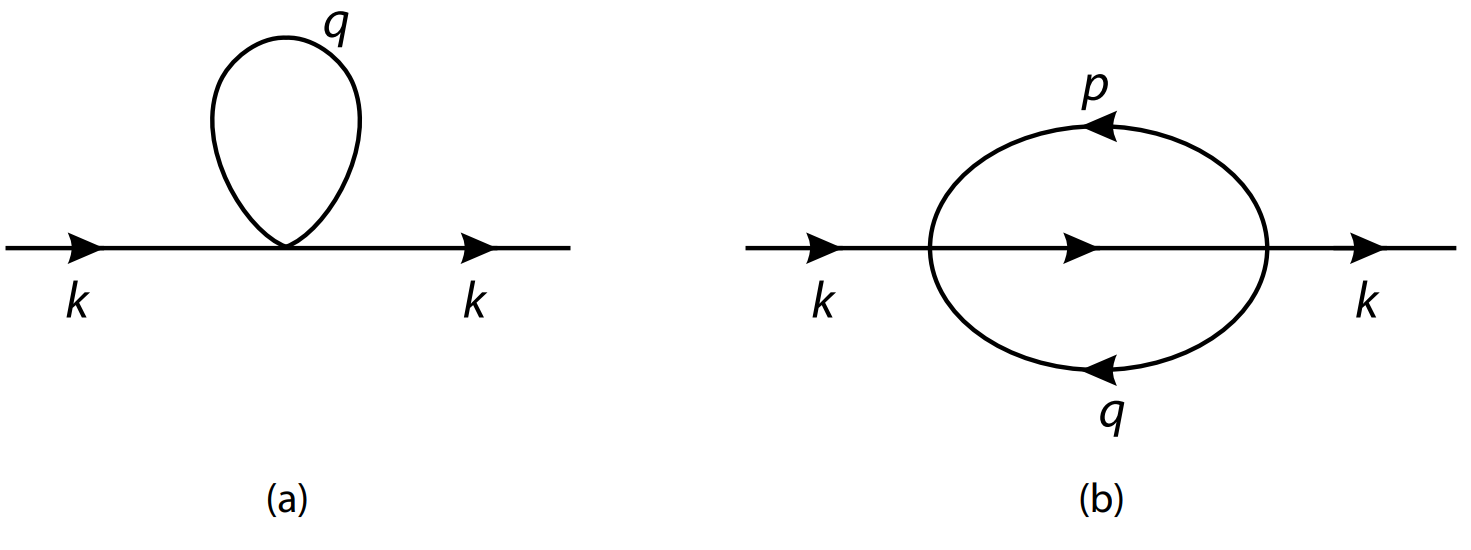
\includegraphics[scale=0.3]{mesons-phi-4}
\end{figure}

The amplitude associated with the first diagram has the form
\begin{align}
\mathcal{M}_1 \propto -i\lambda \int^\Lambda \f{d^4q}{(2\pi)^4}  \f{i}{q^2 - m^2 + i\epsilon}.
\end{align}
since there is one loop of variable momentum $q$. Because we are integrating over four dimensions of $q$ and taking away two dimensions of $q$, we get that this amplitude depends \textit{quadratically} on the cutoff $\Lambda$, but not on $k^2$. \\

On the other hand, the second diagram has a double integral because there are two variable momenta. There are two vertices and three internal lines, so
\begin{align}
\mathcal{M}_2 \propto (-i\lambda)^2 \iint^\Lambda \f{d^4p}{(2\pi)^4}\f{d^4q}{(2\pi)^4} \f{i}{p^2 - m^2 + i\epsilon} \f{i}{q^2 - m^2  + i\epsilon} \f{i}{(p+q+k)^2 - m^2  + i\epsilon}.
\end{align}
We see that we are integrating over 8 total dimensions of momentum, but taking away 6, so this integral depends quadratically on the cutoff $\Lambda$ as well. \\

We also notice that this integral is a function of $k^2$. So (by Lorentz invariance) we can expand it has the series
\begin{align}
D + Ek^2 + Fk^4 + \dots
\end{align}
$D$ must have the same dimension as the integral, so it depends quadratically on $\Lambda$. $E$ can be obtained by differentiating with respect to $k$ twice. This decreases the power of $q,p$ in the integrand by 2 (since the power 2 now becomes 4) and so $E$ depends logarithmically on $\Lambda$ (the integral now looks like $\int d^8x\,1/x^8$). Similarly, we can reason that $F$ looks like the integral $\int d^8x\,1/x^10$ since we need to differentiate with respect to $k$ 4 times, increasing the power of $q,p$ in the exponential by $4$. All this means that $F$ converges and is cutoff-independent. Therefore, we know that $F$ and higher order terms of $k^2$ converge and are $\Lambda$-independent as well. We, then, don't have to worry about them.\\

With this, $\mathcal{M}_2$ is both quadratically and logarithmically cutoff-dependent. Now, suppose we do a \textbf{mass renormalization} by shifting the energy-momentum-mass:
\begin{align}
\f{1}{k^2 - m^2} \to \f{1}{(1+b)k^2 - (m^2 - a)}.
\end{align} 
Obviously the pole in $k^2$ is now shifted to 
\begin{align}
\boxed{m^2_P \equiv m^2 + \delta m^2 \equiv (m^2 - a)(1+b)^{-1}}
\end{align}
We refer to this as the \textbf{physical mass}. With this, we can write the propagator (in momentum space of course) as
\begin{align}
\boxed{\f{1}{k^2 - m^2} \to \f{(1+b)^{-1}}{k^2 - m^2_P}}
\end{align}


Notice here that the residue of the pole in this propagator is no longer 1 but $(1+b)^{-1}$. What is this shift in residue? \\

We note that the coefficient of $k^2$ in $1/\D(k)$ is identically 1 \textit{because} the coefficient of $(1/2)(\p \phi)^2$ is identically 1 in the Lagrangian density. Let's elaborate a little bit. Recall that the spacetime propagator is defined as the \textit{inverse} of the operator $(\square + m^2)$. It follows from here and some properties of Gaussian integrals that the propagator in momentum space has the form $1/(k^2 - m^2)$. This is essentially the derivation we did very early on. So, we see that there is certainly no guarantee that with higher order corrections included the coefficient of $(1/2)(\p \phi)^2$ in an effective $\lag$, say $\lag_{\text{eff}}$, will stay at 1. \\

In fact, by inspection, the coefficient is shifted from 1 to $(1+b)$. This is called \textbf{wavefunction renormalization}, or \textbf{field renormalization}. 






\subsubsection{Physical Perturbation Theory}

The physical perturbation theory is given by
\begin{align}
\boxed{ \lag = \f{1}{2}(\p \phi)^2 + \f{1}{2}m^2 \phi^2 - \f{\lambda_P}{4!}\phi^4 + A(\p \phi)^2 + B\phi^2 + C\phi^4.} 
\end{align}


This theory basically says for each order of $\phi$ in the regular Lagrangian, there is a perturbative term $A$, $B$, or $C$ of the same order the perturbative Lagrangian. This perturbative Lagrangian also carries the physical coupling constant $\lambda_P$ instead of the theoretical $\lambda$. \\



Here's how the theory works: The Feynman rules are as before, but with the crucial different that  the coupling constant is $\lambda_P$, and the propagator has the form
\begin{align}
\f{i}{k^2 - m_P^2 + i\epsilon},
\end{align}
where the physical mass is used instead. The last three terms with coefficients $A$, $B$, and $C$ are called \textbf{counterterms}. These coefficients are determined \textit{iteratively} as we go to higher and higher order in perturbation theory. These perturbations are represented as crosses in Feynman diagrams:
\begin{figure}[!htb]
	\centering
	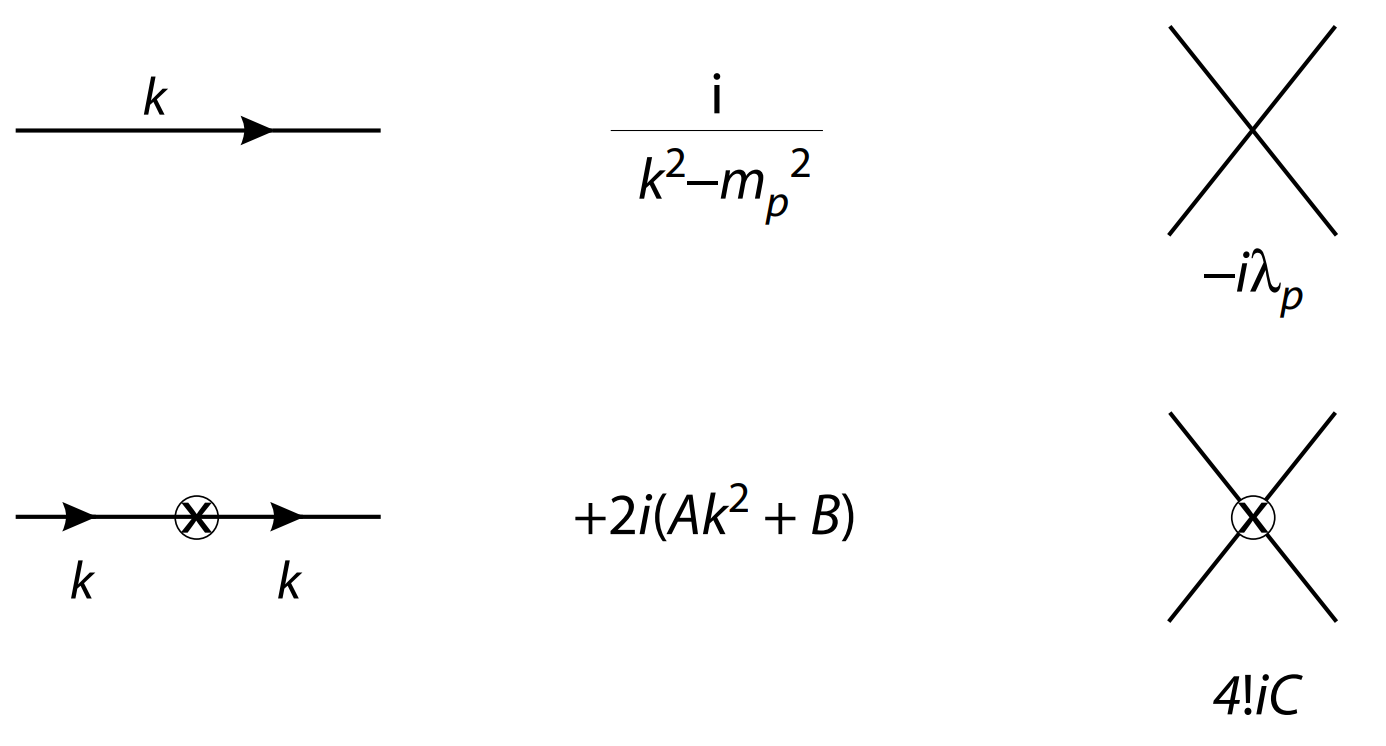
\includegraphics[scale=0.2]{crosses}
\end{figure}\\

We note that all momenta are integrated up to cutoff. \\

The coefficients $A$, $B$, $C$ are determined iteratively as follows. Suppose they are determined up to order $\lambda_P^N$. Let these values be $A_N$, $B_N$, and $C_N$. We then draw all diagrams that appear in order $\lambda_P^{N+1}$. We determine $A_{N+1}$, $B_{N+1}$, and $C_{N+1}$ by requiring that the propagator calculated to the order $\lambda^{N+1}_{P}$ has a pole at $m_p$ with a residue equal to 1, and that the meson=meson scattering amplitude evaluated at some specified values of the kinematic variables has the value $-i\lambda_P$. We note that there are exactly 3 conditions to determine the these three unknown coefficients.










\subsubsection{Degree of Divergence - Power Counting}




\noindent \textbf{Definition:} A diagram is said to have a superficial degree of divergence $D$ if it diverges as $\Lambda^D$. A logarithmic divergence $\log \Lambda$ counts as $D=0$. \qed \\

\noindent \textbf{$\phi$-Theorem:} For a diagram with $B_E$ external $\phi$ lines, the degree of divergence is given by
\begin{align}
\boxed{D = 4 - B_E}
\end{align}\qed \\


\noindent \textit{Proof by Zee:} The proof of this theorem follows from simple power counting. In addition to $B_E$ and $D$, let us define $B_I$ as the number of internal lines, $V$ as the number of vertices (where 4 lines meet), and $L$ as the number of loops. \\

The number of loops is just the number of $\int d^4k/(2\pi)^4$ that we have to do, i.e., it is the number of \textit{independent} internal momenta. Each internal line carries with it a momentum to be integrated over, so we seem to have $B_I$ integrals to do. However, the actual number of integrals to be done to reduced by the momentum conservation delta function associated with the vertices, one to each vertex. By assumption, there are $V$ delta functions, with one of them is associated with the conservation momentum of the entire diagram. It follows that the number of loops is
\begin{align}
L = B_I - (V - 1).
\end{align}


Now, for each vertex, there are four lines. Each external line comes out of one vertex. Each internal line connects two vertices. Thus we have
\begin{align}
4V = B_E + 2B_I.
\end{align}

Finally, for each loop there is a $\int d^k$ while for each internal line there is a $i/(k^2 -m^2 + i\epsilon)$, bringing the powers of momentum down by $2$. So,
\begin{align}
D = 4L - 2B_I.
\end{align}
Putting these relationship together, we obtain
\begin{align}
{D = 4- B_E}
\end{align}
as desired. \qed\\


\noindent \textit{Proof by Me:} I find my proof more intuitive. But I'm of course biased. \underline{To show:}
\begin{align}
D = 4 - B_E
\end{align}
where $D$ is the degree of divergence and $B_E$ is the number of external lines. Well, we know that the number $D$, or the number of divergence is equal to the total number of momentum dimensions in the integral measure, minus the total number of momentum dimensions in the denominator of the integrand, which is a product of propagators. In general, the scattering amplitude integral as the form
\begin{align}
\int \dots \int d^4 p_1 \dots d^4 p_n \lc \f{i}{k^2} \rc^{n'}. 
\end{align} 

So we first have
\begin{align}
D = 4n - 2n'.
\end{align}

Now, what are $n$ and $n'$? $n$ is the total number of integrals, which is equal to the number of ``momentum unknowns'' or ``internal momentum variables'' in a Feynman diagram. This number is completely determined by the number of vertices $V$ and internal lines $B_I$. If we associate to each internal line a variable momentum then we have $B_I$ variables to integrate over, but for each vertex there are two internal lines going out/in to it, so the number of variables is reduced by $V-1$. Note that we only consider internal lines going either in or out of a vertex to avoid double-counting. Thus we have 
\begin{align}
{\#} \text{ integrals } = B_I - (V - 1).
\end{align}

Next, $n'$ is the number of propagators, which is identically the number of internal lines $B_I$. So, 
\begin{align}
D = 4(B_I - (V - 1)) - 2B_I = 2(2 + B_I - 2V).
\end{align}
Okay, but we often know the number of external lines $B_E$, and also know that the total number of lines is 4 times the number of vertices (4 lines per vertex) minus the number of internal lines $B_I$ (accounting for double counting), so
\begin{align}
B_E + B_I = 4V - B_I \iff 2(2 + B - 2V) = 4 - 2B_E. 
\end{align}
Therefore,
\begin{align}
D = 4 - B_E.
\end{align}
\qed\\
















\textbf{Example.} Consider the attached diagram
\begin{figure}[!htb]
	\centering
	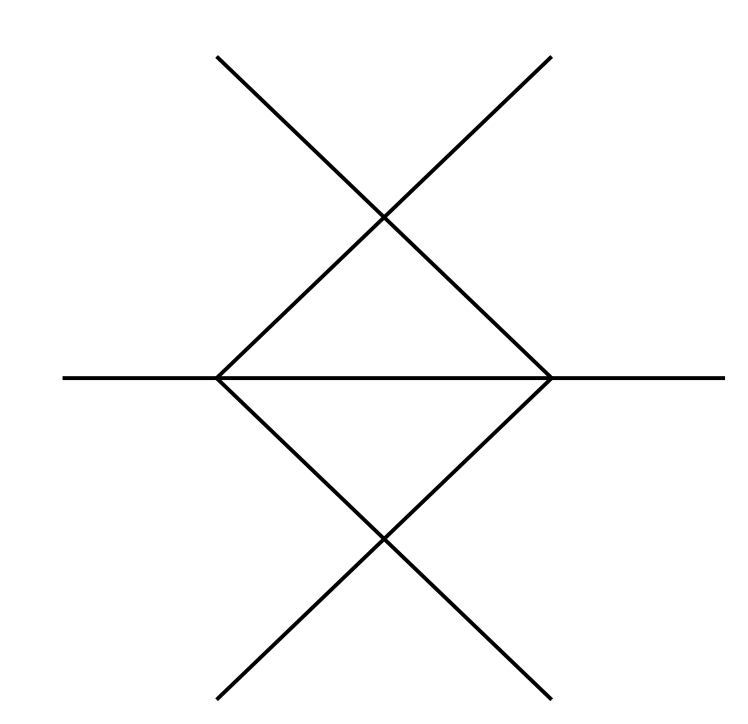
\includegraphics[scale=0.3]{div-count}
\end{figure}\\


By inspection, we have $B_E = 6$. So the theorem says $D = -2$. But we can also verify that this is true. Consider particles coming in from below. Then we have only 2 unknown variable momenta (since the momentum on the internal line in the middle is completely determined by the outgoing momenta and two variable momenta directly above and below). This means we integrate over 8 dimensions of momentum, while carrying 5 propagators, each with $-2$ dimensions of momentum. This means the degree of divergence is $8 - 10 = -2$. So things work as expected.






\subsubsection{Degree of Divergence with Fermions}



The theorem is modified for a different kind of particles. In this case, we have fermions instead of mesons like last time. \\

Consider the following Lagrangian for fermions, called the Yukawa theory
\begin{align}
\lag = \bar{\psi}(i\gamma^\mu \p_\mu - m_P)\psi + \f{1}{2}[(\p \phi)^2 - \mu^2_P \phi^2] - \lambda_P \phi^4 + f_P \phi \bar{\psi}\psi.
\end{align}


Here we have $F_I$ and $F_E$ as the number of internal and external lines as before, but there are two kinds of coupling: $\lambda$ and $f$. Also recall that $[\phi] = 1$ and $[\psi] = 3/2$. We now want to express $D$ in terms of external lines: bosonic external lines $B_E$ and fermionic external lines $F_E$. \\


It turns out that 
\begin{align}
\boxed{D = 4 - B_E - \f{3}{2}F_E}
\end{align}
So the degree of divergence for this theory has an extra dependence on the number of external fermionic lines. \\

To prove this, we will need to know what the fermion propagators are, but since we haven't discussed fermionic propagator up to this point I will present the proof later in this section. However, we can get a feel for why this holds by looking at some Feynman diagrams with fermions and photons. First, we have that vertex amplitudes are assigned as 
\begin{figure}[!htb]
	\centering
	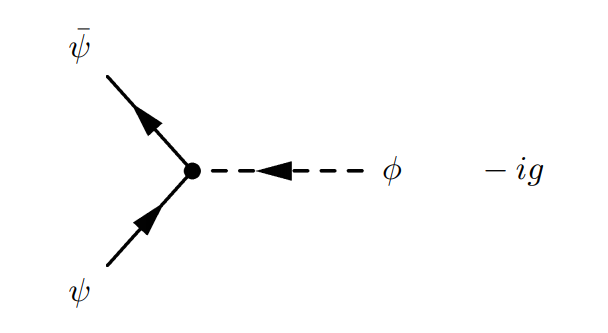
\includegraphics[scale=0.4]{fermi}
\end{figure}\\

With this, some simple Feynman diagrams with no loops look  like
\begin{figure}[!htb]
	\centering
	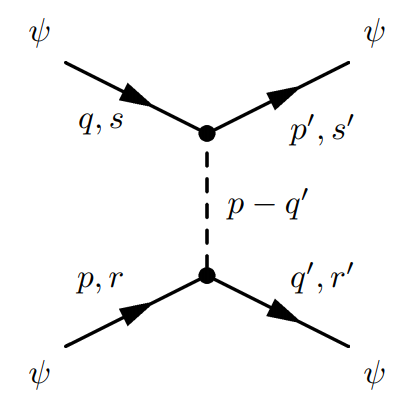
\includegraphics[scale=0.4]{fermi-diagram}
\end{figure}\\

or (with photon lines)
\begin{figure}[!htb]
	\centering
	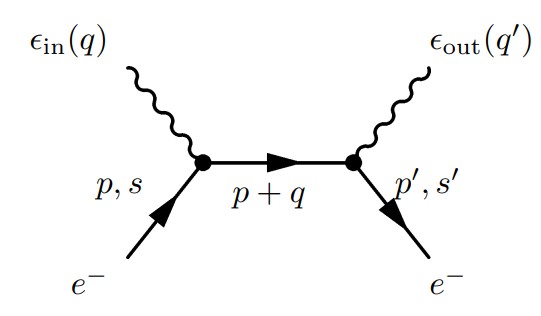
\includegraphics[scale=0.4]{compton}
	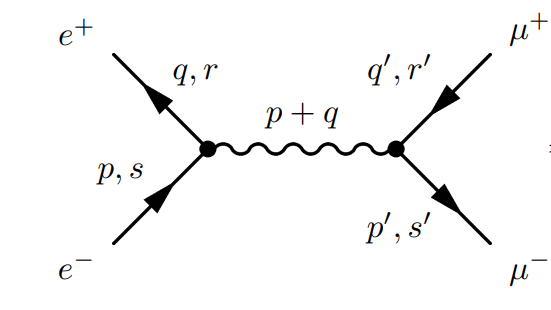
\includegraphics[scale=0.4]{fermi-gen}
\end{figure}\\













\textit{Proof:} Here we show that in fact in Yukawa theory
\begin{align}
D = 4 - B_E - \f{3}{2}F_E.
\end{align}  
The number of loop integrals is given by the number of independent four-momenta in a given diagram. Each propagator has its own four-momentum, while each vertex enforces four-momentum conservation. However, there always remains one overall four-momentum conservation of the diagram.
Hence,
\begin{align}
L = P_f + P_s - V_Y - V_\lambda + 1
\end{align}
where $L$ is the number of loop integrals, $P_f$, $P_s$ the number of fermion or scalar
propagators, respectively, $V_Y$ the number of Yukawa vertices, and $V_\lambda$ is the number of $\phi^4$ vertices. Since each
Yukawa vertex comes with two fermion lines and one scalar line,
\begin{align}
V_Y = \f{1}{2}(2P_f + N_f)
\end{align}
Here, $N_f$, $N_s$ are the number of external fermion or scalar lines, respectively. Each propagator is counted twice as it connects two vertices, while an external line connects to only one vertex. The superficial degrees of divergence is
\begin{align}
D = 4L - P_f - 2P_s
\end{align}
since each fermion propagator is associated with $-1$ dimension of momentum, while each scalar propagator is associated with $-2$ dimensions of momentum.\\

From the previous section, we also know that in the $\phi^4$ theory, 
\begin{align}
4V_\lambda = 2B_I + B_E 
\end{align}
where $B_I$ is the number of $\phi^4$-scalar propagators, and $B_E$ is the number of $\phi^4$-external scalar lines. With this, 
\begin{align}
V_Y + 4 V_\lambda = 2P_s + N_s
\end{align}
because each Yukawa vertex is associated with 1 internal/external scalar line and each 4 $\phi^4$ vertices is associated with 2 internal scalar lines and 1 external scalar line.\\

Therefore, 
\begin{align}
D &= 4(P_f + P_s - V_Y - V_\lambda + 1) - P_f - 2P_s \nn\\
&= 4\lp P_f + P_s - \f{1}{2}(2P_f + N_f) - V_\lambda + 1\rp - P_f - 2P_s \nn\\
&= 4\lp P_f + P_s - \f{1}{2}(2P_f + N_f) - \f{1}{4}\lp 2P_s + N_s - V_Y   \rp + 1\rp - P_f - 2P_s \nn\\
&= 4\lp P_f + P_s - \f{1}{2}(2P_f + N_f) - \f{1}{4}\lp 2P_s + N_s - \f{1}{2}(2P_f + N_f)  \rp + 1\rp - P_f - 2P_s\nn\\
&= 4 - N_s - \f{3}{2}N_s.
\end{align}


Thus, 
\begin{align}
\boxed{D = 4 - N_s - \f{3}{2}N_f}
\end{align}\qed\\







Note: \textit{This proof is collected and \textbf{corrected} from Hitoshi's \href{http://hitoshi.berkeley.edu/230A/Yukawa.pdf}{\underline{notes}}. }\\





\textbf{Remark 1:} We notice that both this result and the result from last section are independent of the number of vertices. This means for a given number of external lines, no matter to what order of perturbation theory we go, the superficial degree of divergence remains the same. \\

\textbf{Remark 2:} We also notice that the leading coefficient of $B_E$ and $F_E$ correspond to the dimension of the respective fields: $[\phi] = 1$, and $[\psi] = 3/2$.\\








\subsubsection{Nonrenormalizable field theories}



Suppose we have a theory where
\begin{align}
D = 4 - \f{3}{2}N_f + 2V.
\end{align}
$D$ now depends on $V$. Thus, if we calculate fermion-fermion scattering, for example, the divergence gets worse and worse as we go to higher and higher orders in the perturbation series. This forces us to include more and more counter terms in the Lagrangian. This makes the theory very limited in predictive power. 















\newpage



\subsection{Gauge Invariance: A Photon Can Find No Rest}






\subsubsection{When the central identity blows up}

Recall that the central identity of quantum field theory is
\begin{align}
\boxed{\int \mathfrak{D}[\phi] \exp\lp -\f{1}{2}\phi \cdot K \cdot \phi _ J\cdot \phi 0 V(\phi) \rp = \exp\lp -V\f{\delta }{\delta J} \rp \exp\lp \f{1}{2}J\cdot K^{-1} \cdot J \rp}
\end{align}



For any field theory, we can always gather up all the fields, put them into one column vector, and call the vector $\phi$. We then single out the term quadratic in $\phi$ and write it as $(1/2)\phi \cdot K \cdot \phi$, and call the rest $V(\phi)$. \\

Question: what is $K$ is not invertible? \\

This happens in the Maxwell action:
\begin{align}
\boxed{S(A) = \int d^4x\,\lag = \int d^4x\, \lb \f{1}{2}A_\mu (\p^2 g^{\mu\nu} - \p^\mu \p^\nu)A_\nu + A_\mu J^\mu \rb}
\end{align}
where the matrix $K$ is proportional the differential operator:
\begin{align}
K \propto Q^{\mu\nu} = (\p^2 g^{\mu\nu} - \p^\mu \p^\nu)
\end{align}
We observe that the kernel of $K$ is non-trivial, i.e., for some non-zero vector, say, $\p_\mu \Lambda(x)$, we have
\begin{align}
Q^{\mu\nu}(\p_\nu \Lambda(x)) = \p^2g^{\mu\nu}\p_\nu \Lambda(x) - \p^\mu\p^\nu\p_\nu \Lambda(x) = \p^\mu \p^2 \Lambda(x) - \p^\mu \p^2 \Lambda(x) = 0
\end{align}
where
\begin{align}
\p^2 = \p_\mu \p^\mu= \p^\mu \p_\mu.
\end{align}

And so we conclude $Q^{\mu\nu}$ is not invertible. This is actually no surprise. We have learned from EM that adding a constant to an electrostatic potential makes no change to the electric field. We also learned that in order to ``solve'' for a potential, we have to ``fix'' a reference point. We sort of do the same thing here: we must impose an additional constant on the gauge potential $A^\mu$. This is called ``fixing the gauge.''






\subsubsection{Restricting the functional integral: Faddeev \& Popov}


Suppose we want to evaluate some integral of the form
\begin{align}
I \equiv \int \mathfrak{D}[A]\,e^{iS(A)},
\end{align}
where this can be an ordinary integral or a path integral. We assume further that under the transformation
\begin{align}
A \to A_g 
\end{align}
the integrand and the measure do not change, i.e.,
\begin{align}
S(A) = S(A_g) \hspace{0.5cm} \mathfrak{D}A = \mathfrak{D}A_g.
\end{align}
The set of these transformations form a \textbf{group} (and we can verify this quite easily by checking: ``closure'', ``identity'', ``associativity'', and ``inverse''). We would like to write the integral $I$ in the form 
\begin{align}
I = \int \mathfrak{D}[g]\, J 
\end{align}
where $J$ is independent of $g$. In other words, we want to factor out the redundant integration over $g$. For example, in order to evaluate
\begin{align}
I = \int dxdy\, e^{iS(x,y)}, \hspace{0.5cm} S(x,y) = x^2 + y^2,
\end{align}
we can go to polar coordinates and write
\begin{align}
I = \int rdrd\theta\, e^{ir^2} = \int d\theta\, J = 2\pi J
\end{align}
where
\begin{align}
J = \int dr\,re^{ir^2}
\end{align}
which is completely independent of $\theta$. \\
 
\textbf{Faddeev \& Popov} showed how to do this ``going over to polar coordinates'' in a unified and elegant way. First, we write
\begin{align}
\boxed{1 = \Delta(A) \int \mathfrak{D}[g] \, \delta[f(A_g)]}
\end{align}
This is just a way for us to define $\Delta(A)$, the Faddeev-Popov determinant, which of course depends on the function $f$. From this definition, we can see that
\begin{align}
[\Delta(A_{g'})]^{-1} = \int \mathfrak{D}[g]\,\delta[f(A_{g'g})] = \int\mathfrak{D}[g''] \delta[f(A_{g''})] = [\Delta(A)]^{-1}
\end{align}
from our assumptions about the transformations (of the same group) and defining $g'' = g'g$ and noting $\mathfrak{D}[g''] = \mathfrak{D}[g'']$. In other words, because the transformations change neither the value of $f$ nor the integration measure, we have
\begin{align}
\boxed{\Delta(A) = \Delta(A_g)}
\end{align}
i.e., the Faddeev-Popov determinant is gauge invariant. With this,
\begin{align}
I &= \int \mathfrak{D}[A]\, e^{iS(A)} \nn\\
&= \int \mathfrak{D}[A]\, e^{iS(A)} \times 1 \nn\\
&= \int \mathfrak{D}[A]\, e^{iS(A)} \Delta(A) \int \mathfrak{D}[g] \, \delta[f(A_g)] \nn\\
&= \lp \int \mathfrak{D}[g]\rp \int \mathfrak{D}[A]\,e^{iS(A)}\Delta(A)\delta[f(A_g)]
\end{align}
Since $\Delta(A)$ is invariant under transformations, we can write
\begin{align}
\boxed{I = \lp \int \mathfrak{D}[g]\rp \int \mathfrak{D}[A]\,e^{iS(A)}\Delta(A)\delta[f(A)]}
\end{align}
where we have made the transformation $A \to A_{g^{-1}}$. \\

So, the group integration $\int \mathfrak{D}[g]$ has been factored out. \\

The Faddeev-Popov argument is an alternative to Feynman argument regarding evaluating $\Z$. The Faddeev-Popov method is useful in Einstein theory. 




\subsubsection{Fixing the electromagnetic gauge}


We will now apply Faddeev-Popov to electromagnetism. We notice that the transformation that leaves the EM action invariant is
\begin{align}
A_\mu \to A_\mu - \p_\mu \Lambda.
\end{align}
This means we can't find the photon propagator (i.e., the inverse of the differential operator) unless we fix this gauge (i.e., making this differential operator at least one-to-one).\\

To do this, we notice that the original integral
\begin{align}
 I &= \int \mathfrak{D}[A]\, e^{iS(A)} = \lp \int \mathfrak{D}[g]\rp \int \mathfrak{D}[A]\,e^{iS(A)}\Delta(A)\delta[f(A)]
\end{align}
is not explicitly dependent on $f$ despite its appearance in the second equality. So, we are free to choose $f$. In particular, let us choose
\begin{align}
f(A) = \p A - \sigma
\end{align}
where $\sigma = \sigma(x)$. Because $I$ is ultimately independent of $\sigma$, we can integrate $I$ with an arbitrary functional of $\sigma$. Let this functional be
\begin{align}
e^{-(i/2\xi)\int d^4x\,\sigma^2(x)}.
\end{align}
With this, we turn the Faddeev-Popov crank:
\begin{align}
[\Delta(A)]^{-1} \equiv \int \mathfrak{D}[g]\,\delta[f(A_g)] = \int\mathfrak{D}[\Lambda]\,\delta[\p A - \p^2 \Lambda - \sigma].
\end{align}
If we set $f(A) = \p A - \sigma = 0$, then 
\begin{align}
\Delta A \sim \lb\int \mathfrak{D}[\Lambda] \delta(\p^2\Lambda)\rb^{-1}
\end{align}
which doesn't depend on $A$ and cancels with the $\int\mathfrak{D}[\Lambda]$ in the $I$ integral. And so
\begin{align}
I \sim \int\mathfrak{D}[A]e^{iS(A)}\delta(\p A - \sigma).
\end{align}
Integrating over $\sigma(x)$ to obtain
\begin{align}
\Z &= \int\mathfrak{D}[\sigma] e^{-(i/2\xi)\int d^4x\, \sigma^2(x)}\int \mathfrak{D}[A]e^{iS(A)}\delta(\p A - \sigma)\nn\\
&= \int \mathfrak{D}[A]e^{iS(A) - (i/2\xi)\int d^4x\,(\p A)^2}.
\end{align}
Thus, the action is effectively
\begin{align}
S_\text{eff} = S(A) - \f{1}{2\xi}\int d^4x\, (\p A)^2
\end{align}
where 
\begin{align}
S(A) = \int d^4x\,\lag = \int d^4x\, \lb \f{1}{2}A_\mu (\p^2 g^{\mu\nu} - \p^\mu \p^\nu)A_\nu + A_\mu J^\mu \rb.
\end{align}
So we find after some simple simplifications that
\begin{align}
\boxed{S_\text{eff} = \int d^4x\, \lc \f{1}{2}A_\mu \lb \p^2 g^{\mu\nu} - \lp 1-\f{1}{\xi} \rp\p^\mu \p^\nu \rb A_\nu + A_\mu J^\mu \rc}
\end{align}
And so we replace $Q^{\mu\nu}$ by
\begin{align}
Q^{\mu\nu}_\text{eff} = \p^2 g^{\mu\nu} - \lp1 - \f{1}{\xi} \rp\p^\mu \p^\nu.
\end{align}
In momentum space, 
\begin{align}
Q^{\mu\nu}_\text{eff,k} = -k^2 g^{\mu\nu} + \lp 1 - \f{1}{\xi} \rp k^\mu k^\nu.
\end{align}
This operator has an inverse. It is straightforward to verify that
\begin{align}
Q^{\mu\nu}_\text{eff,k}\lb -g_{\nu\lambda} + (1-\xi)\f{k_\nu k_\lambda}{k^2} \rb\f{1}{k^2} = \delta^\mu_\lambda.
\end{align}
And so we can choose the photon propagator to be
\begin{align}
\boxed{\f{-i}{k^2}\lb g_{\nu\lambda} - (1-\xi)\f{k_\nu k_\lambda}{k^2} \rb}
\end{align}
















































\newpage


\subsection{Field Theory without Relativity}




\subsubsection{Nonrelativistic limit of QFT}

In this section we learn how to take the nonrelativistic limit of QFT. The Lorentz invariant scalar field theory is given by
\begin{align}
\lag = (\p \Phi^\dagger) (\p \Phi) - m^2 \Phi^\dagger\Phi - \lambda(\Phi^\dagger\Phi)^2
\end{align}
with $\lambda > 0$. This describes interacting bosons, so it should also contain physics of slow moving bosons. \\


Let's now consider the (relativistic) Klein-Gordon equation:
\begin{align}
(\square + m^2)\Phi = 0
\end{align}
for a free scalar field. A mode with energy $E = m + \epsilon$ would oscillate in time as
\begin{align}
\Phi \propto e^{-iEt}.
\end{align}
In the nonrelativistic limit, the kinetic energy $\epsilon \ll m$, so we can write
\begin{align}
\Phi(\vec{x},t) = e^{-imt}\phi(\vec{x},t)
\end{align} 
where $\phi(\vec{x},t)$ oscillates much more slowly than $e^{-imt}$. Since $\Phi(\vec{x},t)$ solves the Klein-Gordon equation we have
\begin{align}
0 &= (\square + m^2)e^{-imt}\phi(\vec{x},t) \nn\\
&=  (\p_t^2 - \laplacian + m^2)e^{-imt}\phi \nn\\
&= \p_t^2(e^{-imt}\phi) - e^{-imt}\laplacian\phi + e^{-imt}m^2\phi \nn\\
&= \p_t[(-im\phi + \p_t\phi)e^{-imt}] - e^{-imt}\laplacian\phi + e^{-imt}m^2\phi \nn\\
&= e^{-imt}[-im(-im\phi + \p_t\phi) + (-im\p_t \phi + \p_t^2\phi)] - e^{-imt}\laplacian\phi + e^{-imt}m^2\phi \nn\\
&= (-m^2\phi + m^2 \phi) -2im\p_t\phi + \p_t^2\phi -\laplacian \phi \nn\\
&\approx -2im\p_t\phi - \laplacian \phi. \hspace{0.5cm} (\p_t^2\phi \to 0 \hspace{0.5cm}\epsilon\ll m)
\end{align} 
So we recover the Schr\"{o}dinger equation:
\begin{align}
i\p_t \phi = -\f{1}{2m}\laplacian \phi.
\end{align}


With this result, we can take the nonrelativistic limit of QFT by plugging 
\begin{align}
\Phi(\vec{x},t) = \f{1}{\sqrt{2m}} e^{-imt}\phi(\vec{x},t)
\end{align}
into the Lagrangian in the beginning, where the factor $1/\sqrt{2m}$ is only for convenience. We will leave the spatial derivatives untouched and only look at the time derivative piece of the Lagrangian:
\begin{align}
\p_t \Phi^\dagger \p_t \Phi - m^2 \Phi^\dagger \Phi &= \f{1}{2m}\lc
\lb im\phi^\dagger + \p_t \phi^\dagger \rb
\lb -im\phi + \p_t \phi\rb
- m^2\phi^\dagger\phi
\rc \nn\\
&\approx \f{i}{2}\lp \phi^\dagger \p_t \phi - \p_t\phi^\dagger \phi \rp.
\end{align}
With
\begin{align}
\p_t(\phi^\dagger\phi) = \p_t \phi^\dagger \,\phi + \phi^\dagger \p_t \phi \implies \p_t \phi^\dagger \,\phi = \p_t(\phi^\dagger\phi) - \phi^\dagger \p_t \phi\to -\phi^\dagger \p_t\phi
\end{align}
we argue that $\phi^\dagger\phi$ no longer has any time dependence because of the conjugation. So we can just set this term to zero.
\begin{align}
\lag &= (\p \Phi^\dagger) (\p \Phi) - m^2 \Phi^\dagger\Phi - \lambda(\Phi^\dagger\Phi)^2 \nn\\
&= \f{i}{2}\lp \phi^\dagger \p_t \phi - \p_t\phi^\dagger \phi \rp - \f{1}{2m}\p_i\phi^\dagger \p_i \phi - \f{\lambda}{4m^2}(\phi^\dagger\phi)^2\nn\\
&= i \phi^\dagger \p_t \phi - \f{1}{2m}\p_i\phi^\dagger \p_i \phi - \f{\lambda}{4m^2}(\phi^\dagger\phi)^2.
\end{align}
We note that the spatial derivatives carry a minus sign because of the Minkowskian metric.








\newpage



\section{Gravity and Beyond}




\subsection{Gravity as a Field Theory}


Recall the Einstein-Hilbert action for gravity:
\begin{align}
S = \f{1}{16\pi G}\int d^4x\,\sqrt{-g}R \equiv \int d^4x\,\sqrt{-g}M_P^2 R
\end{align}
where $g = \det(g_{\mu\nu})$, $R$ is the scalar curvature, and $G$ is Newton's constant. \\

The Riemann curvature tensor is given by
\begin{align}
\tensor{R}{^\lambda_{\mu\nu\kappa}} = \p_\nu \Gamma^\lambda_{\mu\kappa} - \p_\kappa\Gamma^\lambda_{\mu\nu} + \Gamma^\sigma_{\mu\kappa}\Gamma^\lambda_{\nu\sigma} - \Gamma^\sigma_{\mu\nu}\Gamma^\lambda_{\kappa\sigma}.
\end{align}
The Christoffel symbols are constructed out of the metric tensor:
\begin{align}
\Gamma^\lambda_{\mu\nu} = \f{1}{2}g^{\lambda\rho}(\p_\nu g_{\rho\mu} + \p_\mu g_{\rho\nu} - \p_\rho g_{\mu\nu}).
\end{align}
The Ricci tensor is a contraction of the Riemann tensor:
\begin{align}
R_{\mu\kappa} = \tensor{R}{^\nu_{\mu\nu\kappa}}
\end{align}
and the scalar curvature is a contraction of the Ricci tensor
\begin{align}
R = g^{\mu\nu}R_{\mu\nu}.
\end{align}
Varying $S$, i.e., with $\delta S = 0$, we get the Einstein field equation:
\begin{align}
R_{\mu\nu} - \f{1}{2}g_{\mu\nu}R = -8\pi GT_{\mu\nu}
\end{align}
     


\subsubsection{Gravity as a field theory}
When we write the metric as Minkowskian plus a perturbation piece (weak-field expansion):
\begin{align}
g_{\mu\nu} = \eta_{\mu\nu} + h_{\mu\nu}
\end{align}    
the Einstein tensor becomes
\begin{align}
G_{\mu\nu} = \f{1}{2}\lp  \p_\sigma\p_\mu \tensor{h}{^\sigma_\nu} + \p_\nu \p_\sigma \tensor{h}{^\sigma_\mu}- \p_\mu\p_\nu h - \square h_{\mu\nu} - \eta_{\mu\nu}\p_\rho\p_\lambda h^{\rho\lambda} + \eta_{\mu\nu}\square h  \rp
\end{align}
and so the action becomes (schematically)
\begin{align}
S = \int d^4x\, \f{1}{16\pi G}(\p h \p h + h\p h \p h + h^2\p h \p h + \dots)
\end{align}
where the Lorentz indices have been suppressed and second derivatives have been written out in terms like $\p h \p h$, etc. The field $h^{\mu\nu}(x)$ describes a graviton in flat pace and is to be treated like any other field. The first term $\p h \p h$ is analogous to $\p \phi \p \phi$ or $\p A \p A$ in the usual field theory, and so it also governs how the graviton propagates. The terms cubic and higher in $h$ determine the interaction of the graviton with itself. \\

Gravity is not renormalizable. The Einstein-Hilbert action is an infinite series in the graviton field $h_{\mu\nu}$ due to the presence of $\sqrt{-g}$ and the inverse of $g_{\mu\nu}$. \\

With the stress-energy tensor being
\begin{align}
T^{\mu\nu}(x) = -\f{2}{\sqrt{-g}}\f{\delta S_M}{\delta g_{\mu\nu}(x)}
\end{align}
as defined in \href{https://huanqbui.com/LaTeX projects/Classical_Fields_Theory/HuanBui_ClassicalFieldTheory.pdf}{\underline{the CFT notes}}, in Sec 8.3, the coupling of the graviton to matter (in the weak field limit of course) can be included by adding the term
\begin{align}
- \int d^4x\, \f{1}{2}h_{\mu\nu}T^{\mu\nu}
\end{align}
to the action so that schematically,
\begin{align}
S = \int d^4x\, \lb \f{1}{16\pi G}(\p h \p h + h \p h \p h + h^2 \p h \p h + \dots) + (hT + \dots)\rb
\end{align}
We can rescale $h^{\mu\nu} \to \sqrt{G} h^{\mu\nu}$ as absorb $16\pi$ whenever convenient so that we can just write the action as
\begin{align}
S = \int d^4x\, (\p h \p h  + \sqrt{G}h \p h \p h + Gh^2\p h \p h + \dots + \sqrt{G} h T)
\end{align}
Because the Planck mass $M_P \equiv 1/\sqrt{16\pi G} $ is enormous, we see once again that the coupling strength of the graviton to itself and any other field is very weak.



\subsubsection{The weak field action}
     
     
From Sean Carroll's \textit{Spacetime \& Geometry}, or from the \href{https://huanqbui.com/LaTeX projects/Classical_Fields_Theory/HuanBui_ClassicalFieldTheory.pdf}{CFT notes}, we have seen the weak field action:
\begin{align}
S = \int d^4x\, \sqrt{-g}\lag = \int d^4x\, \lag
\end{align}
where
\begin{align}
\lag = \f{1}{2}\lb(\p_\mu h^{\mu\nu})(\p_\nu h) - (\p_\mu h^{\rho\sigma})(\p_\rho \tensor{h}{^\mu_\sigma}) + \f{1}{2} \eta^{\mu\nu}(\p_\mu h^{\rho\sigma})(\p_\nu h_{\rho\sigma})   - \f{1}{2} \eta^{\mu\nu}(\p_\mu h)(\p_\nu h) \rb.
\end{align}

We know that when requiring $\delta S = 0 \iff \delta S / \delta h^{\mu\nu} = 0$, i.e., the variational derivative of $S$ with respect to $h^{\mu\nu}$ is zero, we get the Einstein tensor $G_{\mu\nu}$ given by
\begin{align}
G_{\mu\nu} &= R_{\mu\nu} - \f{1}{2}\eta_{\mu\nu}R \nonumber\\
&= \f{1}{2}\lp  \p_\sigma\p_\mu \tensor{h}{^\sigma_\nu} + \p_\nu \p_\sigma \tensor{h}{^\sigma_\mu}- \p_\mu\p_\nu h - \square h_{\mu\nu} - \eta_{\mu\nu}\p_\rho\p_\lambda h^{\rho\lambda} + \eta_{\mu\nu}\square h  \rp
\end{align}

Let's check this in xACT, as an exercise in indexing and of course in using xACT. Here are the things we will need to do, in order: (1) importing the packages, (2) defining the manifold, (3) turning on the metric variations option, (4) defining the metric $\eta_{\mu\nu}$ (don't worry about making it Minkowskian), (5) defining the perturbation $h_{\mu\nu}$, (6) defining the Lagrangian, (7) taking the variational derivative of the Lagrangian with VarD (assuming $\sqrt{-\eta} = 1$, of course).
\begin{lstlisting}
... (import packages here)
...
DefManifold[M4, 4, {a, b, c, d, e, f, i, k, l, m, n}]

DefMetricPerturbation /. Options@DefMetric

DefMetric[-1, \[Eta][-a, -b], CD, {"%", "\[Del]"}]

DefMetricPerturbation[\[Eta], h, \[Epsilon]]

Lag := (1/
2)*((CD[-m][h[LI[1], m, n]])*(CD[-n][h[LI[1], -c, c]]) - (CD[-m][
h[LI[1], c, d]])*(CD[-c][h[LI[1], m, -d]]) + (1/2)*\[Eta][m, 
n]*(CD[-m][h[LI[1], c, d]])*(CD[-n][h[LI[1], -c, -d]]) - (1/
2)*\[Eta][m, 
n]*(CD[-m][h[LI[1], c, -c]])*(CD[-n][h[LI[1], d, -d]]))

(VarD[h[LI[1], c, d], CD][Lag*Sqrt[-Det\[Eta][]]]/
Sqrt[-Det\[Eta][]]) /. delta[-LI[1], LI[1]] -> 1 // 
ExpandPerturbation // ContractMetric // ToCanonical
\end{lstlisting}
Here's what we get:
\begin{figure}[!htb]
	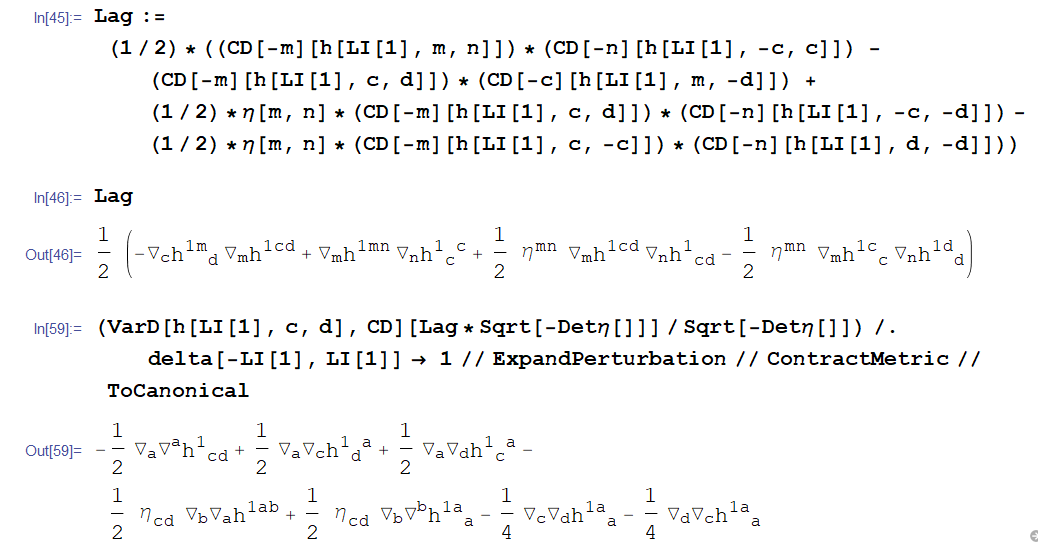
\includegraphics[scale=0.4]{lag-weak}
\end{figure}

Putting this back into \LaTeX{} after doing some manual contractions/simplifications, plus noting that the covariant derivative here is just the regular partial derivatives, we find that
\begin{align}\label{GGG}
G_{\mu\nu} = \f{1}{2}\lp -\square h_{\mu\nu} + \p_\sigma \p_\nu \tensor{h}{^\sigma_\mu}  
+ \p_\sigma \p_\mu \tensor{h}{^\sigma_\nu} 
- \eta_{\mu\nu}\p_\lambda \p_\sigma h^{\lambda\sigma} + \eta_{\mu\nu}\square h - \p_\mu\p_\nu h\rp
\end{align}
which matches exactly with the Einstein tensor $G_{\mu\nu}$ provided earlier.\\


Note that when calling the perturbation metric $h_{\mu\nu}$ in xACT, make sure that you are calling it by \textbf{h[LI[order],-m,-n]}, so that xACT knows you \textit{mean} to call the perturbation metric.\\



Thus we confirm that the Lagrangian above gives the correct Einstein tensor. But how is it found? Consider a general coordinate transformation:
\begin{align}
x'^\mu \to x^\mu - \epsilon^\mu(x).
\end{align}
Then the metric changes according to 
\begin{align}
g'^{\mu\nu} = \f{\p x'^\mu}{\p x^a} \f{\p x'^\nu}{\p x^b} g^{ab},
\end{align}
where, as before,
\begin{align}
g^{\mu\nu} = \eta^{\mu\nu} - h^{\mu\nu} +\dots
\end{align}
How does $h_{\mu\nu}$ transform under this transformation? Well, we first have that
\begin{align}
\f{\p x'^\mu}{\p x^a}= \f{\p}{\p x^a} (x^\mu - \epsilon^\mu(x)) = \delta^\mu_a - \p_a \epsilon^\mu.
\end{align}
And so treating $\p_\mu \epsilon_\nu$ as the same order as $h^{\mu\nu}$ we find
\begin{align}
g'^{\mu\nu} &= \f{\p x'^\mu}{\p x^a} \f{\p x'^\nu}{\p x^b}\lp \eta^{ab} - h^{ab} \rp\nn\\
&= (\delta^\mu_a - \p_a\epsilon^\mu)(\delta^\nu_b - \p_b\epsilon^\nu)\lp \eta^{ab} - h^{ab} \rp\nn\\
&\approx (\delta^\mu_a - \p_a\epsilon^\mu)(\eta^{a\nu} - h^{a\nu} - (\p_b e^\nu)\eta^{ab}+\dots\nn)\\
&\approx \eta^{\mu\nu} - h^{\mu\nu} - (\p_a \epsilon^\nu)\eta^{\mu a} - (\p_b \epsilon^\mu)\eta^{b\nu}.
\end{align}
Next, we lower the index to get $h'_{\mu\nu}$:
\begin{align}
\eta_{c\mu}\eta_{d\nu}g'^{\mu\nu} &= \eta_{c\mu}\eta_{d\nu}\lp \eta^{\mu\nu} - h^{\mu\nu} - (\p_a \epsilon^\nu)\eta^{\mu a} - (\p_b \epsilon^\mu)\eta^{b\nu} \rp\nn\\
\eta_{cd} - h'_{cd} &= \eta_{cd} - h_{cd} - (\p_a \epsilon_d)\delta^a_c - (\p_b\epsilon_c)\delta^b_c\nn\\
h'_{cd} &= h_{cd} + \p_c \epsilon_d +  \p_d \epsilon_c. 
\end{align}
And so we have
\begin{align}
\boxed{h'_{\mu\nu}= h_{\mu\nu} + \p_\mu \epsilon_\nu + \p_\nu \epsilon_\mu}
\end{align}
and of course as a side product:
\begin{align}
\boxed{h'^{\mu\nu} = h^{\mu\nu} + \p^\mu \epsilon^\nu + \p^\nu \epsilon^\mu}
\end{align}
and so the infinitesimal change in $h_{ab}$ or $h^{ab}$ is
\begin{align}
&\boxed{\delta h_{\mu\nu} = \p_\mu \epsilon_\nu + \p_\nu \epsilon_\mu}\\
&\boxed{\delta h^{\mu\nu} = \p^\mu \epsilon^\nu + \p^\mu \epsilon^\mu}
\end{align}
which, by the way, are actually the Lie  derivatives of the perturbative metric $h_{\mu\nu}$ and its inverse $h^{\mu\nu}$. These formulas represent the change of the metric perturbation under an infinitesimal diffeomorphism along the vector field $\epsilon^\mu$. \\ 

Since we want to get $G_{\mu\nu}$ that is linear in $h_{\mu\nu}$, we look for quadratic terms in $h$ and in $\p$. Lorentz invariance tells us that there are four possible terms. So the action has the form
\begin{align}
\boxed{S = \int d^4x\,(a\p_\lambda h^{\mu\nu}\p^\lambda h_{\mu\nu} + b \p_\lambda \tensor{h}{^\mu_\mu} \p^\lambda \tensor{h}{^\nu_\nu} + c\p_\lambda h^{\lambda \nu}\p^\mu h_{\mu\nu} + d\p^\mu\tensor{h}{^\lambda_\lambda}\p^\nu h_{\mu\nu} )}
\end{align}
where $a,b,c,d$ are unknown constants. Next, we require that $\delta S / \delta h_{\mu\nu} =0 $ with $\delta h_{\mu\nu} = \p_\mu \epsilon_\nu + \p_\nu \epsilon_\mu$. This should give 3 equations with 4 unknowns. Upon writing three unknowns in terms of the remaining unknown we can find the form of the Lagrangian. In the end, we should be able to fix the action up to an overall constant factor.\\

With $\delta S = 0$, we bring the $\delta$ into the integrand and let $\delta \lag = 0$. The next step is to do variational derivatives with respect to $h_{\mu\nu}$ on each term in the integrand. We shall proceed, first with the first term:
\begin{align}
\delta(\p_\lambda h^{\mu\nu}\p^\lambda h_{\mu\nu}) &= \p_\lambda (\delta h^{\mu\nu})(\p^\lambda h_{\mu\nu}) + (\p_\lambda h^{\mu\nu})\p^\lambda( \delta h_{\mu\nu} )\nn\\
&= \p_\lambda (\p^\mu \epsilon^\nu + \p^\nu \epsilon^\mu)(\p^\lambda h_{\mu\nu}) + (\p_\lambda h^{\mu\nu})\p^\lambda (\p_\mu \epsilon_\nu + \p_\nu \epsilon_\mu)\nn\\
&= \p_\lambda (\p^\mu \epsilon^\nu + \p^\nu \epsilon^\mu)(\p^\lambda h_{\mu\nu}) + (\p^\lambda h_{\mu\nu})\p_\lambda (\p^\mu \epsilon^\nu + \p^\nu \epsilon^\mu)\nn\\
&= 2\p_\lambda (\p^\mu \epsilon^\nu + \p^\nu \epsilon^\mu)(\p^\lambda h_{\mu\nu})\nn\\
&= 4[\p_\lambda (\p^\mu \epsilon^\nu)](\p^\lambda h_{\mu\nu}),
\end{align}
where the fourth equality follows from the symmetry $\mu\leftrightarrow \nu$ in a summation. Zee says 
\begin{align}
[\p_\lambda (\p^\mu \epsilon^\nu)](\p^\lambda h_{\mu\nu}) \sim \epsilon^\nu \p^2 \p^\mu h_{\mu\nu}
\end{align}
from ``integrating by parts'' freely. It turns out we have to integrate by parts twice to get this equality. We shall proceed with the first integration by parts with respect to some measure $d\omega$ which we are not going to worry about. We shall also assume that everything vanishes when evaluated at infinity and that differential operators such as $\delta, \p_\alpha, \p^\beta, \square$ commute.
\begin{align}
\int d\omega \, \p_\lambda[(\p^\mu \epsilon^\nu)(\p^\lambda h_{\mu\nu})] &= \int d\omega\, [\p_\lambda(\p^\mu\epsilon^\nu)](\p^\lambda h_{\mu\nu}) + \int d\omega\, (\p^\mu\epsilon^\nu)(\p_\lambda \p^\lambda h_{\mu\nu}) \nn\\
(\p^\mu \epsilon^\nu)(\p^\lambda h_{\mu\nu})\bigg\vert_{-\infty}^\infty&= \int d\omega\, [\p_\lambda(\p^\mu\epsilon^\nu)](\p^\lambda h_{\mu\nu}) + \int d\omega\, (\p^\mu\epsilon^\nu)(\p_\lambda \p^\lambda h_{\mu\nu})\nn\\
0  &=  \int d\omega\, [\p_\lambda(\p^\mu\epsilon^\nu)](\p^\lambda h_{\mu\nu}) + \int d\omega\, (\p^\mu\epsilon^\nu)(\p_\lambda \p^\lambda h_{\mu\nu})\nn\\
\implies [\p_\lambda(\p^\mu \epsilon^\nu)] (\p^\lambda h_{\mu\nu})  &= -\p^\mu \epsilon^\nu \p_\lambda \p^\lambda h_{\mu\nu}.
\end{align}
We evaluate this term (again) by integration by parts, again over some arbitrary measure $d\omega$ we won't worry about:
\begin{align}
\p^\mu (\epsilon^\nu \p_\lambda \p^\lambda h_{\mu\nu})\bigg\vert_{-\infty}^\infty &= \int d\omega\, \p^\mu \epsilon^\nu \p_\lambda \p^\lambda h_{\mu\nu} + \int d\omega\,  \epsilon^\nu \p_\lambda \p^\lambda \p^\mu h_{\mu\nu}\nn\\
0 &= \int d\omega\, \p^\mu \epsilon^\nu \p_\lambda \p^\lambda h_{\mu\nu} + \int d\omega\,  \epsilon^\nu \p_\lambda \p^\lambda \p^\mu h_{\mu\nu}\nn\\
\implies -\p^\mu \epsilon^\nu \p_\lambda \p^\lambda h_{\mu\nu} &= \epsilon^\nu \underbrace{\p_\lambda \p^\lambda}_{\square} \p^\mu h_{\mu\nu}.
\end{align}
And so, we have for the first term:
\begin{align}
\boxed{\delta (\p_\lambda h^{\mu\nu} \p^\lambda h_{\mu\nu}) = 4e^\nu \square \p^\mu h_{\mu\nu}} 
\end{align}


Moving on the second term:
\begin{align}
\delta[(\p_\lambda h)( \p^\lambda h)] &= \delta[(\p_\lambda \tensor{h}{^\mu_\mu})( \p^\lambda \tensor{h}{^\nu_\nu})]\nn\\
&= (\p_\lambda \delta\tensor{h}{^\mu_\mu})( \p^\lambda \tensor{h}{^\nu_\nu}) + (\p_\lambda \tensor{h}{^\mu_\mu})( \p^\lambda \delta\tensor{h}{^\nu_\nu}).
\end{align}
We notice that this term is very similar to the first term, except for the ``position of the index of $h$.'' That is to say, we are finding $\delta$ of the contraction. However, we can always write
\begin{align}
&\tensor{h}{^\mu_\mu} = \eta_{\mu x}h^{\mu x}\\
&\tensor{h}{^\nu_\nu} = \eta^{\nu y}h_{\nu y}.
\end{align}
From here we can do some mental prepping for what to come: the metric is constant in the eyes of $\delta$, so we can just pull the $\eta$'s out to the left and treat them as constants. By doing this, we're left with $\eta^{\mu x}\eta_{\nu y}$ times a term of the form similar to the first term except for the appearance of the indices $x,y$. However, by symmetry arguments, we should be able to get
\begin{align}
\delta[(\p_\lambda h)( \p^\lambda h)] = 4\epsilon^\nu \square \p_\nu h
\end{align}
where the factor of $4$ is explicitly shown here for reasons we will see later. We shall see why this is true. First we write the contractions in terms of the original tensor $h$ times the metric 
\begin{align}
\delta[(\p_\lambda h)( \p^\lambda h)] &= \lp\eta_{\mu x}\eta^{\nu y}\rp\delta[(\p_\lambda h^{\mu x})(\p^\lambda h_{\nu y})].
\end{align}
Invoking the fact that
\begin{align}
&\delta h^{ab} = \p^a \epsilon^b + \p^b \epsilon^a \nn\\
&\delta h_{ab} = \p_a \epsilon_b + \p_b \epsilon_a 
\end{align}
and the $b\leftrightarrow a$ symmetry argument in a summation, we find
\begin{align}
\delta[(\p_\lambda h)( \p^\lambda h)] &= 2\lp\eta_{\mu x}\eta^{\nu y}\rp [(\p_\lambda \p^\mu \epsilon^x)(\p^\lambda h_{\nu y}) + (\p^\lambda h_{\mu x})(\p_\lambda \p^\nu \epsilon^y)]\nn\\
&= 2\lp\eta_{\mu x}\eta^{\nu y}\rp [(\p_\lambda \p^\mu \epsilon^x)(\p^\lambda h_{\nu y}) + (\p_\lambda h^{\mu x})(\p^\lambda \p_\nu \epsilon_y)]\nn\\
&= 4\lp\eta_{\mu x}\eta^{\nu y}\rp[(\p_\lambda \p^\mu \epsilon^x)(\p^\lambda h_{\nu y})]\nn\\
&= 4(\p_\lambda \p^\mu \epsilon_\mu)(\p^\lambda h)\nn\\
&= 4(\p_\lambda \p_\mu \epsilon^\mu)(\p^\lambda h).
\end{align}
Time to integrate by parts (again over some measure $d\omega$ we won't worry about)
\begin{align}
\p_\lambda[(\p_\mu \epsilon^\mu)(\p^\lambda h)]\bigg\vert_{-\infty}^\infty  &= \int d\omega\,(\p_\lambda \p_\mu \epsilon^\mu)(\p^\lambda h) + \int d\omega\,(\p_\mu \epsilon^\mu)\square h\nn\\
0 &= \int d\omega\,(\p_\lambda \p_\mu \epsilon^\mu)(\p^\lambda h) + \int d\omega\,(\p_\mu \epsilon^\mu)\square h\nn\\
\implies (\p_\lambda \p_\mu \epsilon^\mu)(\p^\mu h) &= -(\p_\mu \epsilon^\mu)\square h.
\end{align}
We integrate by parts again:
\begin{align}
\p_\mu[\epsilon^\mu \square h]\bigg\vert_{-\infty}^\infty &= \int d\omega\,(\p_\mu \epsilon^\mu)\square h + \int d\omega\, e^\mu \square \p_\mu h\nn\\
0 &= \int d\omega\,(\p_\mu \epsilon^\mu)\square h + \int d\omega\, \epsilon^\mu \square \p_\mu h\nn\\
\implies (\p_\mu \epsilon^\mu)\square h &=-\epsilon^\mu \square \p_\mu h.
\end{align}
So we have for the second term
\begin{align}
\boxed{\delta[(\p_\lambda h)( \p^\lambda h)] = 4\epsilon^\nu \square \p_\nu h}
\end{align}
Very nice! What about the third term? We claim:
\begin{align}
\delta[(\p_\lambda h^{\lambda \nu})( \p^\mu h_{\mu\nu})] = 2\epsilon^\nu\square\p^\mu h_{\mu\nu} + 2\epsilon^\nu \p_\nu \p^\lambda  \p^\mu h_{\mu\lambda}.
\end{align}
The only way to verify this is integration by parts (surprise!). But first we have to let $\delta$ act on the $h$'s and write things out in terms of $\epsilon$'s:
\begin{align}
\delta[(\p_\lambda h^{\lambda \nu})( \p^\mu h_{\mu\nu})] = (\p_\lambda(\p^\lambda \epsilon^\nu + \p^\nu \epsilon^\lambda))(\p^\mu h_{\mu\nu}) + (\p_\lambda h^{\lambda\nu})(\p^\mu(\p_\mu \epsilon_\nu + \p_\nu \epsilon_\mu)).
\end{align}
We will treat these two terms differently, despite the symmetry. For the first term, we simply integrate by parts twice to get
\begin{align}
(\p_\lambda(\p^\lambda \epsilon^\nu + \p^\nu \epsilon^\lambda))(\p^\mu h_{\mu\nu}) &= 2(\p_\lambda\p^\lambda \epsilon^\nu)(\p^\mu h_{\mu\nu}) \nn\\
&= -2(\p^\lambda \epsilon^\nu)(\p_\lambda\p^\mu h_{\mu\nu}) \nn\\
&= 2(\epsilon^\nu)(\p^\lambda \p_\lambda\p^\mu h_{\mu\nu})\nn\\
&= 2(\epsilon^\nu)\square\p^\mu h_{\mu\nu}.
\end{align}
We recognize that, for the second term, by exchanging the indices  $\mu \to \nu \to \lambda \to \mu$, then appropriately lowering and raising the indices on the second term, then use the $\lambda \leftrightarrow \nu$ symmetry argument in the Lie derivative summation, we get
\begin{align}
(\p_\mu h^{\mu\lambda})(\p^\nu(\p_\lambda \epsilon_\nu + \p_\nu \epsilon_\lambda)) &= (\p^\mu h_{\mu\lambda})(\p_\nu(\p^\lambda \epsilon^\nu + \p^\nu \epsilon^\lambda))\nn\\
&= 2(\p^\mu h_{\mu\lambda})(\p_\nu\p^\lambda \epsilon^\nu).
\end{align}
From here, we will integrate by parts twice to get what we want. I won't be showing all the steps here because we can now do this integration by parts ``internally:''
\begin{align}
2(\p^\mu h_{\mu\lambda})\p_\nu (\p^\lambda \epsilon^\nu) = -2(\p_\nu\p^\mu h_{\mu\lambda})(\p^\lambda \epsilon^\nu) = 2\epsilon^\nu \p^\lambda \p_\nu \p^\mu h_{\mu\lambda} = 2\epsilon^\nu \p_\nu \p^\lambda  \p^\mu h_{\mu\lambda},
\end{align} 
where the last equality follows from the fact that these differential operators commute. Recognize the pattern in the first two equalities? Every time we integrate by parts, we essentially let one derivative act on another factor (say let $\p_\nu$ act on the $\p h$ instead of on $\epsilon$). Since the total derivative is zero when evaluated at infinity, this new quantity is equal to minus the original quantity. We keep doing this until all derivatives are sandwiched between $\epsilon^\nu$ and $h_{\mu\lambda}$. \\

So we have for the third term
\begin{align}
\boxed{\delta[(\p_\lambda h^{\lambda \nu})( \p^\mu h_{\mu\nu})] = 2\epsilon^\nu\square\p^\mu h_{\mu\nu} + 2\epsilon^\nu \p_\nu \p^\lambda  \p^\mu h_{\mu\lambda}}
\end{align}

What about the fourth term? Once again we have a contraction, which means we need to write it out in terms of the metric $\eta$, then pull it outside of the derivative since it is just a constant in the eyes of $\delta$. We also invoke the symmetry argument once again with derivatives of the $\epsilon$'s. So,
\begin{align}
\delta[\p^\mu\tensor{h}{^\lambda_\lambda}\p^\nu h_{\mu\nu} ] &= \delta[\eta_{\lambda x}\p^\mu h^{\lambda x}  \p^\nu h_{\mu\nu}]\nn\\
&= (\eta_{\lambda x})\delta[ \p^\mu h^{\lambda x} \p^\nu h_{\mu\nu}]\nn\\
&= (\eta_{\lambda x})\lc \p^\mu(\p^\lambda \epsilon^x + \p^x \epsilon^\lambda)\p^\nu h_{\mu\nu} + \p^\mu h^{\lambda x}  \p^\nu (\p_\mu \epsilon_\nu + \p_\nu \epsilon_\mu) \rc\nn\\
&= 2(\p^\mu\p^\lambda \epsilon_\lambda) \p^\nu h_{\mu\nu} + (2\p^\mu h) \p^\nu(\p_\mu\epsilon_\nu).
\end{align}
Integrate by parts the first term (twice) to get
\begin{align}
2 (\p^\mu \p^\lambda \epsilon_\lambda)\p^\nu h_{\mu\nu} = 2\epsilon_\lambda \p^\lambda \p^\mu \p^\nu h_{\mu\nu}.
\end{align}
Integrate by parts the second term (twice) to get
\begin{align}
(2\p^\mu h) \p^\nu(\p_\mu\epsilon_\nu) &= 2\epsilon^\nu \square \p_\nu h.
\end{align}
So we have
\begin{align}
\boxed{\delta[\p^\mu\tensor{h}{^\lambda_\lambda} \p^\nu h_{\mu\nu}] = 2\epsilon_\lambda \p^\lambda \p^\mu \p^\nu h_{\mu\nu} + 2\epsilon_\nu\square \p^\nu h =  2\epsilon^\lambda \p_\lambda \p^\mu \p^\nu h_{\mu\nu}  + 2\epsilon^\nu\square \p_\nu h}
\end{align}
Very nice! Putting everything we've done so far together, we find
\begin{align}
&\,\delta(a\p_\lambda h^{\mu\nu}\p^\lambda h_{\mu\nu} + b \p_\lambda h \p^\lambda h + c\p_\lambda h^{\lambda \nu}\p^\mu h_{\mu\nu} + d\p^\mu h \p^\nu h )\nn\\
= &\,4a(\epsilon^\nu \square \p^\mu h_{\mu\nu}) + 4b(\epsilon^\nu \square \p_\nu h) + c (2\epsilon^\nu\square\p^\mu h_{\mu\nu} + 2\epsilon^\nu \p_\nu \p^\lambda  \p^\mu h_{\mu\lambda}) \nn \\ &\,\,\,\,\,+ 2d(\epsilon^\lambda \p_\lambda \p^\mu\p^\nu h_{\mu\nu}) + 2d(\epsilon^\nu \square \p_\nu h)\nn\\
= &\,(4a+2c)(\epsilon^\nu \square \p^\mu h_{\mu\nu}) + (4b + 2d)(\epsilon^\nu \square \p_\nu h) + (2c+ 2d)(\epsilon^\nu \p_\nu \p^\lambda\p^\mu h_{\lambda\mu})\nn\\
= & \,0.
\end{align} 
When holds when we let $a = 1/2$, then $c = -1$, so $d = 1$, which implies $b = -1/2$.
Thus the correct action up to an overall factor is
\begin{align}
\boxed{S = \int d^4x\, \f{1}{2}\p_\lambda h^{\mu\nu}\p^\lambda h_{\mu\nu} -\f{1}{2} \p_\lambda h \p^\lambda h -\p_\lambda h^{\lambda \nu}\p^\mu h_{\mu\nu} + \p^\mu h\p^\nu h_{\mu\nu}}
\end{align}
So we have successfully constructed the linearized action.\\

Thus even if we had never heard of the Einstein-Hilbert action we could still determine the action gravity in the weak field limit by requiring that the action be invariant under the transformation
\begin{align}
x^\mu \to x'^\mu - \epsilon^\mu(x)
\end{align}
or equivalently 
\begin{align}
\delta h_{\mu\nu} = h'_{\mu\nu} - h_{\mu\nu} = \p_\mu \epsilon_\nu +\p_\nu \epsilon_\mu. 
\end{align}
So based on our argument in the previous section, we can now write the weak field expansion of the action $S$ as
\begin{align}
\boxed{S_{\text{wfg}} = \int d^4x\, \lp \f{1}{32\pi G}\mathcal{I} - \f{1}{2}h_{\mu\nu}T^{\mu\nu} \rp}
\end{align}
where
\begin{align}
\mathcal{I} = \f{1}{2}\p_\lambda h^{\mu\nu}\p^\lambda h_{\mu\nu} -\f{1}{2} \p_\lambda h \p^\lambda h -\p_\lambda h^{\lambda \nu}\p^\mu h_{\mu\nu} + \p^\mu h\p^\nu h
\end{align}
and $T_{\mu\nu}$ is the stress-energy tensor associated with matter. 






\subsubsection{Graviton propagator}


From the previous section we see that the weak field action $S_{\text{wfg}}$ has the same quadratic structure of all the field theories we have studied, and so the graviton propagator is once again the inverse of a differential operator. But just as in Maxwell's theory the relevant differential operator in the Einstein-Hilbert theory does not have an inverse because of the ``gauge invariance,'' i.e., under a transformation the action remains invariant. In other terms, we see that the kernel of the differential operator is not trivial, i.e., it is not one-to-one and therefore cannot have a well-defined inverse. \\

To deal with this, we need to rely on the Faddeev-Popov method. Recall that the Faddeev-Popov method allows us to split our integration over physically distinct configurations and those over gauge orbits.\\

We observe that by adding 
\begin{align}
\lp \p^\mu h_{\mu\nu} - \f{1}{2}\p_\nu \tensor{h}{^\lambda_\lambda} \rp^2
\end{align}
to the invariant Lagrangian
\begin{align}
\f{1}{2}\p_\lambda h^{\mu\nu}\p^\lambda h_{\mu\nu} -\f{1}{2} \p_\lambda \tensor{h}{^\mu_\mu} \p^\lambda \tensor{h}{^\nu_\nu} -\p_\lambda h^{\lambda \nu}\p^\mu h_{\mu\nu} + \p^\mu \tensor{h}{^\lambda_\lambda}\p^\nu h_{\mu\nu}
\end{align}
we get
\begin{align}
&\,\f{1}{2}\p_\lambda h^{\mu\nu}\p^\lambda h_{\mu\nu} -\f{1}{2} \p_\lambda \tensor{h}{^\mu_\mu} \p^\lambda \tensor{h}{^\nu_\nu} -\cancel{\p_\lambda h^{\lambda \nu}\p^\mu h_{\mu\nu}} + \cancel{\p^\mu \tensor{h}{^\lambda_\lambda}\p^\nu h_{\mu\nu}}\nn\\
&\,\,\,\,\,+ \cancel{(\p^\mu h_{\mu\nu})(\p^\lambda h_{\lambda \nu})} - \cancel{\p^\mu h_{\mu\nu}\p_\nu \tensor{h}{^\lambda_\lambda}} + \f{1}{4}(\p_\nu h)(\p^\nu h)\nn\\
=&\, \f{1}{2}\p_\lambda h^{\mu\nu}\p^\lambda h_{\mu\nu} -\f{1}{4} \p_\lambda \tensor{h}{^\mu_\mu} \p^\lambda \tensor{h}{^\nu_\nu}. 
\end{align}
the weak field action effectively becomes
\begin{align}
\boxed{S_\text{wfg} = \int d^4x\, \f{1}{2}\lb \f{1}{32\pi G}\lp \p_\lambda h^{\mu\nu} \p^\lambda h_{\mu\nu} - \f{1}{2}\p_\lambda h\p^\lambda h \rp - h_{\mu\nu}T^{\mu\nu} \rb}
\end{align}
Why is this addition justified? Recall in the subsection \textit{Gauge Invariance: A Photon Can Find No Rest} where we introduced the Faddeev-Popov trick, we find that by adding $(\p A)^2$ to the Lagrangian we were able to replace the original action by a new action whose Lagrangian contains has a differential operator with an inverse. We are doing a similar thing here. \\

But of course we can't just add whatever we want to the Lagrangian and expect it to describe the same physics. One way to keep the Lagrangian the same is to require whatever we are adding to be zero. In our case, the freedom in choosing $h_{\mu\nu}$ makes this a necessary condition, which means
\begin{align}
\p^\mu h_{\mu\nu} - \f{1}{2}\p_\nu \tensor{h}{^\lambda_\lambda}  = 0 \iff \boxed{\p^\mu h_{\mu\nu} = \f{1}{2}\p_\nu \tensor{h}{^\lambda_\lambda}}
\end{align} 
This is called the \textbf{harmonic gauge condition}. It turns out that this is the linearized version of
\begin{align}
\p_\mu \lp \sqrt{-g}g^{\mu\nu} \rp = 0.
\end{align}


With these results, we can write the action as
\begin{align}
S_\text{wfg} &= \int d^4x\, \f{1}{2}\lb \f{1}{32\pi G}\lp \p_\lambda h^{\mu\nu} \p^\lambda h_{\mu\nu} - \f{1}{2}\p_\lambda h\p^\lambda h \rp - h_{\mu\nu}T^{\mu\nu} \rb\nn\\
%&= \int d^4x\, \f{1}{2}\lb \f{1}{32\pi G}\lp \p_\lambda h^{\mu\nu} \p^\lambda h_{\mu\nu} - \p^\mu h_{\mu\nu} \p^\lambda h \rp - h_{\mu\nu}T^{\mu\nu} \rb\nn\\
&= \boxed{\f{1}{32\pi G}\int d^4x\, \lb h^{\mu\nu}K_{\mu\nu;\lambda\sigma}(-\p^2)h^{\lambda\sigma} + \mathcal{O}(h^3) \rb}
\end{align}
where
\begin{align}
\boxed{K_{\mu\nu;\lambda\sigma} \equiv \f{1}{2}(\eta_{\mu\lambda}\eta_{\nu\sigma} +\eta_{\mu\sigma}\eta_{\nu\lambda} - \eta_{\mu\nu}\eta_{\lambda\sigma}  )}
\end{align}
where we regard $\lambda\nu$ and $\lambda\sigma$ as two indices. We can work backwards to check writing the action in this form makes sense, but let's not worry too much about that for now.\\

Note that we are dealing with matrices acting in a linear space spanned by symmetric two-index tensors. Thus, the identity matrix is actually
\begin{align}
I_{\mu\nu;\lambda\sigma} \equiv \f{1}{2}(\eta_{\mu\lambda}\eta_{\nu\sigma} + \eta_{\mu\sigma}\eta_{\nu\sigma}).
\end{align}
We can check that
\begin{align}
K_{\mu\nu;\lambda\sigma} \tensor{K}{^{\lambda\sigma}_{;\rho\omega}} = I_{\mu\nu;\rho\omega},
\end{align}
so that
\begin{align}
K^{-1} = K,
\end{align}
similar to how $\eta^{\mu\nu} = \eta_{\mu\nu}$. Thus in the harmonic gauge the graviton propagator in flat spacetime, in momentum space, is given by (up to Newton's constant)
\begin{align}
\boxed{\D_{\mu\nu;\lambda\sigma}(k) = \f{1}{2}\f{K_{\mu\nu;\lambda\sigma}}{k^2 + i\epsilon} = \f{1}{2}\f{\eta_{\mu\lambda}\eta_{\nu\sigma} +\eta_{\mu\sigma}\eta_{\nu\lambda} - \eta_{\mu\nu}\eta_{\lambda\sigma}}{k^2 + i\epsilon}}
\end{align}
where the final $k^2$ comes from the $\p^2$ in the Lagrangian when moving to momentum space, as always.  \\

So there is our graviton propagator, in the weak field limit.




\subsubsection{Newton from Einstein}

Suppose we want to find the equation of motion corresponding to the action given above
\begin{align}
S_\text{wfg} &= \int d^4x\, \f{1}{2}\lb \f{1}{32\pi G}\lp \p_\lambda h^{\mu\nu} \p^\lambda h_{\mu\nu} - \f{1}{2}\p_\lambda h\p^\lambda h \rp - h_{\mu\nu}T^{\mu\nu} \rb.
\end{align}
To find the equation of motion for this theory we take the variational derivative of $S_\text{wfg}$ with respect to $h^{\mu\nu}$. \\

We will rely on xACT to do this. Assuming that the rest has been setup correctly, we will just define the effective Lagrangian, vary it with respect to $h_{\mu\nu}$, and set everything to zero.
\begin{lstlisting}
In[15]:= DefTensor[T[m, n], M4]

During evaluation of In[15]:= ** DefTensor: Defining tensor T[m,n]. 

In[16]:= DefConstantSymbol[G]

During evaluation of In[16]:= ** DefConstantSymbol: Defining constant symbol G. 

In[19]:= LagEff := (1/
2)*( (1/(32*Pi*G))*(CD[-l][h[LI[1], m, n]]*
CD[l][h[LI[1], -m, -n]] - (1/2)*CD[-l][h[LI[1], a, -a]]*
CD[l][h[LI[1], b, -b]]) - h[LI[1], -m, -n]*T[m, n] )

In[20]:= LagEff

Out[20]= 1/2 (- h[
xAct`xTensor`LI[1], -m, -n]  T[m, n] + (-(1/2) CD[-l][
h[
xAct`xTensor`LI[1], a, -a]] CD[l][
h[
xAct`xTensor`LI[1], b, -b]] + CD[-l][
h[
xAct`xTensor`LI[1], m, n]] CD[l][
h[
xAct`xTensor`LI[1], -m, -n]])/(32 G \[Pi]))

In[23]:= (VarD[h[LI[1], c, d], CD][LagEff*Sqrt[-Det\[Eta][]]]/
Sqrt[-Det\[Eta][]]) == 0 /. delta[-LI[1], LI[1]] -> 1 // 
ExpandPerturbation // ContractMetric // ToCanonical
\end{lstlisting}
We quickly find
\begin{figure}[!htb]
	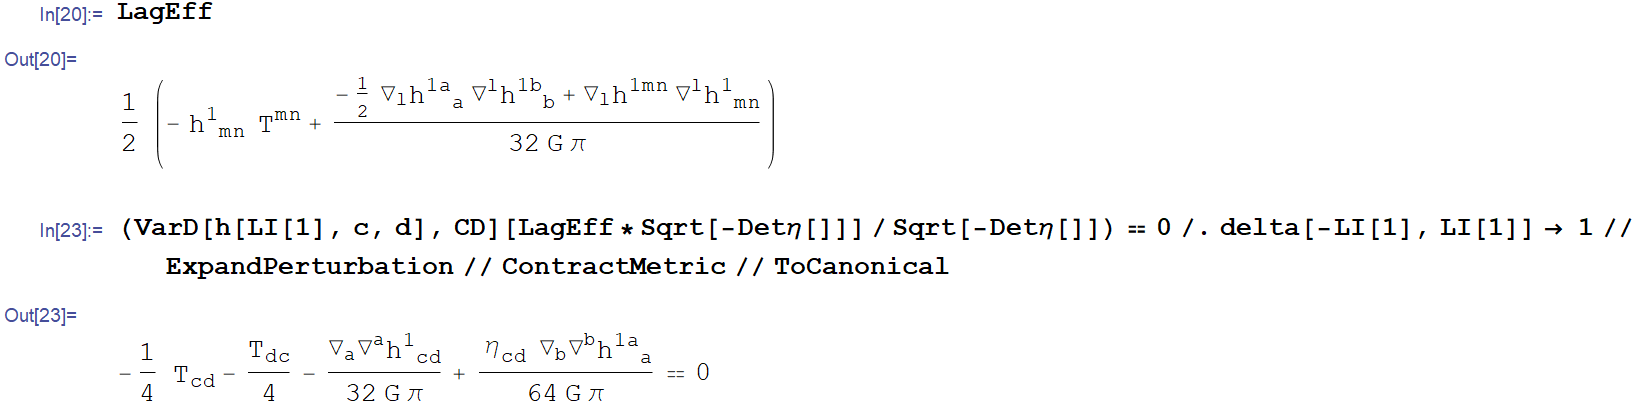
\includegraphics[scale=0.3]{newton-einstein}
\end{figure}
Since the stress-energy tensor is symmetric, we can combine $T_{cd}$ and $T_{dc}$ in the output to get the Euler-Lagrange equation of motion:
\begin{align}
\boxed{\f{1}{32\pi G}(- 2 \square h_{\mu\nu} + \eta_{\mu\nu} \square h) - T_{\mu\nu} = 0}
\end{align}
Easy! Contracting this (i.e., taking the trace):
\begin{align}
\eta_{\mu\nu}\lb\f{1}{32\pi G}(- 2 \square h_{\mu\nu} + \eta_{\mu\nu} \square h) - T_{\mu\nu}\rb &= \f{1}{32\pi G}\lp -2\square h + 4 \square h \rp - T \nn\\
&= \f{1}{16\pi G} \square h - T \nn\\
&= 0.
\end{align}
Therefore
\begin{align}
\square h = 16\pi GT = 16\pi G \eta^{\mu\nu}T_{\mu\nu}.
\end{align}
And so plugging things back into the Euler-Lagrange equation we can find 
\begin{align}
\boxed{\square h_{\mu\nu} = -16\pi G \lp T_{\mu\nu} - \f{1}{2}\eta_{\mu\nu}T \rp}
\end{align}
In the static limit, $T_{00}$ is the dominant component of the stress-energy tensor, and so this equality reduces to
\begin{align}
\boxed{\laplacian{\phi}= 4\pi GT_{00}}
\end{align}
where the Newtonian gravitational potential is $\phi \equiv h_{00}/2$. We have just derived Poisson's equation for $\phi$. 




\subsubsection{The gravity of light}


We now have the objects required for doing perturbative quantum gravity: the propagator, the interactions between gravitons ($h-h$ interactions), and the interactions between gravitons and other matter ($h-T$ interactions). The problem is that we might drown in a sea of indices. \\

Since gravitons not only interact with other fields but also with themselves, we can ask whether light gravitationally affect light. Tolman, Ehrenfest, and Podolsky discovered that in the weak field limit two lights beams moving in the same direction do not interact gravitationally, but two light beams moving in the opposite directions do. What calculation did they do to find this?\\

Consider the scattering of two photons
\begin{align}
k_1 + k_2 \to p_1 + p_2
\end{align}
via the exchange of a graviton. This interaction is given by the Feynman diagram:
\begin{figure}[!htb]
	\centering
	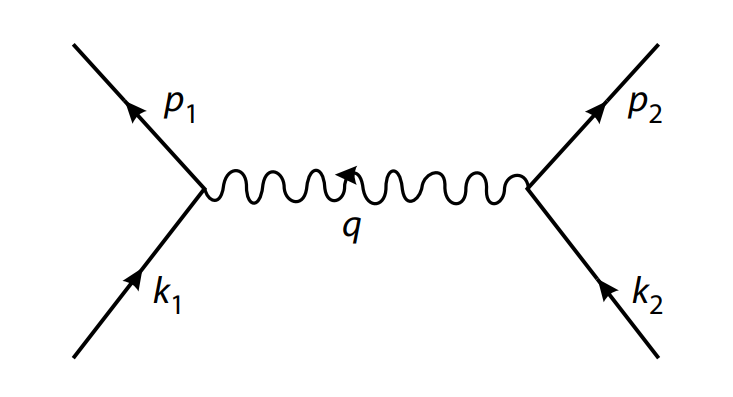
\includegraphics[scale=0.35]{graviton}
\end{figure}
The momentum transfer is
\begin{align}
q \equiv p_1 - k_1.
\end{align}
The Feynman rule for coupling a graviton to two photons can be read off from 
\begin{align}
h^{\mu\nu}T_{\mu\nu} = -h^{\mu\nu}\lp F_{\mu\lambda}\tensor{F}{_\nu^\lambda} - \f{1}{4}\eta_{\mu\nu}F_{\rho\lambda}F^{\rho\lambda} \rp
\end{align}
but all we need is that the interaction involve two powers of spacetime derivatives $\p$ acting on the EM potential $A_\mu$ so that the graviton-photon-photon vertex involves 2 powers of momenta, one from each photon. The scattering amplitude has the schematic form $(k_1p_1)\D(k_2p_2)$ where $\D$ is the propagator. By the form of the propagator
\begin{align}
\D_{\mu\nu;\lambda\sigma}(k) = \f{1}{2}\f{K_{\mu\nu;\lambda\sigma}}{k^2 + i\epsilon} = \f{1}{2}\f{\eta_{\mu\lambda}\eta_{\nu\sigma} +\eta_{\mu\sigma}\eta_{\nu\lambda} - \eta_{\mu\nu}\eta_{\lambda\sigma}}{k^2 + i\epsilon}
\end{align}
we see that the amplitude is the sum of three terms such as $(k_1 \cdot p_1)(k_2\cdot p_2)/q^2$, $(k_1\cdot k_2)(p_1\cdot p_2)/q^2$, and $(k_1\cdot p_2)(k_2 \cdot p_1)/q^2$. According to the Fourier transform, the long distance part of the interaction potential is given by the small $q$ behavior of the scattering amplitude, we need only evaluate these terms in the limit $q\to 0$. This means $k_1 \cdot p_1 \sim k_1 \cdot k_1 = 0$, and $k_1\cdot p_2 = k_1 \cdot (k_1 + k_2 - p_1) \to k_1 \cdot k_2$. So the final amplitude looks like $(k_1 \cdot k_2)(p_1 \cdot p_2)/q^2$. If $k_1$ and $k_2$ point in the same direction, $k_1 \cdot k_2 \sim k_1 \cdot k_1 = 0$, i.e. two photons moving in the same direction do not interact gravitationally. \\

We can also do a rough calculation to justify all this. The stress-energy tensor $T^{\mu\nu}$ of a light beam moving in the $x-$direction has four nonzero components: the energy density $T^{00}$, $T^{x0} = T^{00}$ since photons carry the same energy and momentum, $T^{x0} = T^{0x}$ by symmetry, and $T^{xx} = T^{00}$ since the stress-energy tensor of the EM field is traceless. (Note: $x$ here stands for the $x-$direction, so $T^{x0}$ refers to a \textit{single} component of the tensor). We also know that $h^{00} = h$. The metric around the light beam is given by $g_{00} = 1 + h$, $g_{0x} = g_{x0} = -h$, and $g_{xx} = -1 + h$, and $g_{zz} = g_{yy} = -1$. Consider a photon moving parallel to the light beam. Its world line is determined by
\begin{align}
\f{d^2 x^\rho}{d \zeta^2} = -\Gamma^\rho_{\mu\nu} \f{d x^\mu}{d\zeta} \f{d x^\nu}{d \zeta}.
\end{align}
(This just says light follows a geodesic.) To find whether light gets deflected by another beam of light we wish to calculate $d^2 y / d\zeta^2$ and $d^2 z / d\zeta^2$ and show they are both identically zero. Of course we can just do the $y$ and the $z$ follows by symmetry. We also assume that $dy/d\zeta$, $dz/d\zeta \ll dt/d\zeta$ and $dx/d\zeta$:
\begin{align}
\f{d^2y}{d\zeta^2} = \f{d^2 x^y}{d\zeta^2} &= -\Gamma^y_{\mu\nu} \f{d x^\mu}{d\zeta} \f{d x^\nu}{d \zeta}\nn\\
&= -\f{1}{2}g^{y\rho}\lp \p_\nu g_{\rho\mu} + \p_\mu g_{\rho\nu} - \p_\rho g_{\mu\nu} \rp\f{dx^\mu}{d\zeta} \f{dx^\nu}{d \zeta}, \nn \quad g^{yy} = -1, g^{y\lambda} = 0 \text{ else}\\
&= +\f{1}{2}\lp \p_\nu g_{y\mu} + \p_\mu g_{y\nu} - \p_y g_{\mu\nu} \rp\f{dx^\mu}{d\zeta} \f{dx^\nu}{d \zeta} \nn\\
&= \dots\nn\\
&= -\f{1}{2}(\p_y h)\lb \lp \f{dt}{d\zeta} \rp^2 + \lp \f{dx}{d\zeta} \rp^2 - 2\f{dt}{d\zeta}\f{dx}{d\zeta} \rb\nn\\
&= -\f{1}{2}(\p_y h)\lp \f{dt}{d\zeta} - \f{dx}{d\zeta}   \rp^2 \nn\\
&= 0
\end{align}
since $dt = dx$ for a photon beam traveling in the same direction as the light beam:
\begin{align}
(1+h)dt^2 - 2h\,dtdx - (1-h)dx^2 = 0 \iff dx/dt = \mp \f{1\pm h}{1-h}
\end{align}
and that $y = x^{(2)}$ (2 here is an index). Similarly, we have $d^2z/d\zeta^2  =0$.\\

So we have that the photon's trajectory isn't bent/deflected by light when it is moving in the same direction with the light beam.









\newpage



\section{Massive Gravity}

\subsection{A Brief History}

Massive gravity has a long-winded history. In 1939, Fierz-Pauli wrote down a linearized massive gravity theory for massive spin-2 field $h_{\mu\nu}$. ($j = 2, m_j = -2,-1,0,1,2$). \\

Later in 1970, van Dam, Veltman, and Zakharov (vDVZ) discovered what called the vDVZ discontinuity. They showed that in the $m\to 0$ limit, Fierz-Pauli theory no longer agrees with GR.\\

Then, in 1872 Vainshtein studied non-linear Fierz-Pauli and found a screening mechanism where near some object like the sun for $r < r_V \sim (M / m^4 M_{Pl}^2)^{1/5} = \Lambda_5$ agreement with GR is obtained in the $m \to 0$ limit. \\

In the same year, however, Boulware \& Desen showed that in the nonlinear regime, a ghost mode emerges (BD ghost).\\

In 2003, Arkani-Hamed et al wrote a expository \href{https://arxiv.org/pdf/hep-th/0210184.pdf}{\underline{paper}} on this theory. We will spend some time on this paper.\\

Then, in 2010, de Rham-Gabadadze-Tolley (dRGT) found that for a special non-linear potential in place of the Fierz-Pauli mass term the DB ghost goes away. This new theory is valid up to $\Lambda_5$ cutoff scale. This theory also has self-accelerating solutions. This implies less need for dark energy.



\newpage


\subsection{Quick review of Field Dimensions}
Here we will quickly go over basic field dimensions. We first establish the natural units: $\hbar = c = 1$. With this $E \sim m \sim p \sim \omega$ GeV. $x\sim t \sim 1/E$. We will use mass dimension $m$ as units. With this.
\begin{align}
[x] = [t] =  [K]^{-1} = m^{-1}.
\end{align} 
The action looks something like
\begin{align}
S = \int d^4x\, dt \lag.
\end{align}
$S$ has units of $\hbar = J\cdot s$, so $S$ has no units. So
\begin{align}
[S] = [K]^{0} = m^0.
\end{align}
We can figure out field dimensions from $S$. Relativistically,
\begin{align}
S = \int d^4x\,\lag.
\end{align}
The action is dimensionless, while $[d^4x] = [K]^{-4}$. So
\begin{align}
[\lag] = [K]^{4}.
\end{align}
Now suppose for the scalar field theory
\begin{align}
\lag = \p \phi \p \phi
\end{align}
schematically. Then because $[\p] = [t]^{-1} = [x]^{-1} = [K]$, we find that
\begin{align}
[\phi]= [K].
\end{align}
So, scalars have mass dimension of 1. \\

Next, we look at vector field theory with
\begin{align}
\lag \sim F^{\mu\nu}F_{\mu\nu}
\end{align}
where 
\begin{align}
F_{\mu\nu} = \p_\mu A_\nu - \p_\nu A_\mu.
\end{align}
Since $[\lag] = [K]^4$ and $[\p]= [K]$, we find
\begin{align}
[A_\mu] = [K].
\end{align}
So vector fields also have mass dimension 1. What about a mass term? Suppose
\begin{align}
\lag = \f{1}{2}\p_\mu \phi \p6\mu \phi- \f{1}{2}m^2 \phi^2.
\end{align}
We see that $[m] = [K] = m$ is consistent with $[\phi] = m$ and $[\lag] = [K]^4 = m^4$.\\

What about gravity? What is the dimension of the metric? Well, we look at
\begin{align}
ds^2 = g_{\mu\nu}dX^\mu dX^\nu.
\end{align}
There are two units of length on both sides of the equation so
\begin{align}
[g_{\mu\nu}] = [K]^0,
\end{align}
i.e. assuming Cartesian coordinates, the metric is dimensionless. What about the connections? Christoffel symbols have the form
\begin{align}
\Gamma \sim g \p g.
\end{align}
So 
\begin{align}
[\Gamma] = [\p] = [K].
\end{align}
Riemann curvature tensors look like
\begin{align}
\tensor{R}{^a_{bcd}} \sim \Gamma^2 + \p \Gamma + \dots
\end{align}
so 
\begin{align}
[\tensor{R}{^a_{bcd}}] = [K]^2.
\end{align}
So we find that 
\begin{align}
[\lag_{grav}] = [\tensor{R}{^\mu_\mu}] \neq [K]^4.
\end{align}
It turns out that
\begin{align}
[\lag] \sim \f{1}{16\pi G}[R] = [K]^4.
\end{align}
This means 
\begin{align}
[G] = [K]^{-2}.
\end{align}
This says the Newton's gravitational constant $G$ has mass$^{-2}$ units. With this we can define
\begin{align}
G \equiv \f{1}{m^2_{Pl}},
\end{align}
where $m_{Pl}$ is the Planck mass. In GeV units, $m_{Pl} \sim 10^{19}$ GeV, which is very large, making $G$ very small. \\

Lastly, we notice that gravity has a dimensional constant in its kinetic term, while other fields do not. This makes quantizing/renormalizing gravity difficult. 











\newpage
\subsection{Fierz-Pauli Massive Gravity}

This section focuses on various aspects of Fierz-Pauli massive gravity. The content is based on this \href{https://arxiv.org/abs/1105.3735}{\underline{paper}} by Kurt Hinterbichler. This is my exposition of part II. of the paper, which gives an overview of the original Fierz-Pauli massive gravity. I will follow the paper's layout through and fill in the details wherever I feel necessary.


\subsubsection{The Action \& Fierz-Pauli Tuning}



Recall from earlier we have worked both ways to show the action in linearized gravity (without $T_{\mu\nu}$) up to some overall constant factor is:
\begin{align}
S_{Zee} = \int d^Dx\, \f{1}{2}\p_\lambda h^{\mu\nu}\p^\lambda h_{\mu\nu} -\f{1}{2} \p_\lambda h \p^\lambda h -\p_\lambda h^{\lambda \nu}\p^\mu h_{\mu\nu} + \p^\mu h\p^\nu h_{\mu\nu}.
\end{align}
This is the action obtained from Zee's construction. But to stay close this paper, I will use Sean Carroll's action instead:
\begin{align}
S_{SC} = \int d^Dx\, -\f{1}{2}\p_\lambda h_{\mu\nu} \p^\lambda h^{\mu\nu} + \p_\mu h_{\nu\lambda}\p^\nu h^{\mu\lambda} - \p_\mu h^{\mu\nu}\p_\nu h + \f{1}{2}\p_\lambda h \p^\lambda h.
\end{align}
This action is exactly the same as what Carroll has, up to index permutations.\\

We are familiar with this action, as it describes the (well-known by now) weak field limit. The Fierz-Pauli action is just this with an additional mass term:
\begin{align}
\int d^Dx\, -\f{1}{2}m^2\lp h_{\mu\nu}h^{\mu\nu} - h^2 \rp
\end{align}
hence the name ``massive gravity.'' The full action, then, is
\begin{empheq}[box=\widefbox]{align}
S_{FP} = \int d^Dx\, &-\f{1}{2}\p_\lambda h_{\mu\nu} \p^\lambda h^{\mu\nu} + \p_\mu h_{\nu\lambda}\p^\nu h^{\mu\lambda}\nn\\& - \p_\mu h^{\mu\nu}\p_\nu h + \f{1}{2}\p_\lambda h \p^\lambda h -\f{1}{2}m^2\lp h_{\mu\nu}h^{\mu\nu} - h^2 \rp
\end{empheq}
We wish to show that this action describes a massive spin 2 field (5 d.o.f $= 2s+1$). In the $m=0$ case, we recover the linearized Einstein-Hilbert action with the gauge symmetry:
\begin{align}
\delta h_{\mu\nu} = \p_\mu \epsilon_\nu + \p_\nu \epsilon_\mu
\end{align}
where once again 
\begin{align}
\delta h_{\mu\nu} = h'_{\mu\nu} - h_{\mu\nu}. 
\end{align}
We have actually seen how the action can be constructed from this gauge symmetry.\\

With $m\neq 0$, however, the gauge symmetry is violated. It is clear that
\begin{align}
\delta\lb \f{1}{2}m^2\lp h^{\mu\nu}h_{\mu\nu} + h^2 \rp  \rb &= \f{1}{2}m^2 \lb (\p^\mu \epsilon^\nu + \p^\nu \epsilon^\mu)h_{\mu\nu} + h^{\mu\nu}(\p_\mu\epsilon_\nu + \p_\nu\epsilon_\mu ) - \delta h^2 \rb\nn\\
&= \f{1}{2}m^2\lb 2(\p^\mu \epsilon^\nu + \p^\nu \epsilon^\mu)h_{\mu\nu} - \delta(\tensor{h}{^\mu_\mu}\tensor{h}{^\nu_\nu}) \rb\nn\\
&= \f{1}{2}m^2\lb 4(\p^\mu \epsilon^\nu) h_{\mu\nu} - \eta_{\mu a}\eta^{\nu b}\delta(h^{\mu a}h_{\nu b}) \rb\nn\\
&= \f{1}{2}m^2\lb 4(\p^\mu \epsilon^\nu) h_{\mu\nu} - \eta_{\mu a}\eta^{\nu b}\lc 2(\p^\mu\epsilon^a)h_{\nu b} + 2(\p_\nu \epsilon_b)h^{\mu a}\rc \rb\nn\\
&= \f{1}{2}m^2\lb 4(\p^\mu \epsilon^\nu) h_{\mu\nu} - 4(\p^\mu \epsilon_\mu)h \rb\nn\\
&= 2m^2[(\p^\mu \epsilon^\nu) h_{\mu\nu} - (\p^\mu \epsilon_\mu)h],
\end{align}
which is linearly independent with other terms in the variational Lagrangian $\delta \lag$. This says that
\begin{align}
\delta \lag = 0 \iff m^2 = 0.
\end{align}
But obviously since we explicitly set $m\neq 0$, we must have that $\delta \lag \neq 0$ under $\delta h_{\mu\nu} = \p_\mu \epsilon_\nu + \p_\nu \epsilon_\mu$. So we say the mass term violates this gauge symmetry.\\

The relative coefficient $-1$ between $h^2$ and $h_{\mu\nu}h^{\mu\nu}$ contractions is called the \textit{Fierz-Pauli tuning}. This number is not enforced by any known symmetry. However, any deviation from it, i.e., for any combination
\begin{align}
h_{\mu\nu}h^{\mu\nu} - (1-a)h^2, \quad a \neq 0
\end{align}
results in the action describing a scalar ghost with mass
\begin{align}
\boxed{m_g^2 = -\f{3-4a}{2a}m^2}
\end{align}
and negative kinetic energy in addition to the massive spin 2. We shall show why this is the case with a 2-step argument partially inspired by \href{http://indico.ictp.it/event/a11178/session/6/contribution/3/material/0/0.pdf}{\underline{A. Nicolis}} from ICTP. In Step 1, we show that the Fierz-Pauli tuning has to be $-1$ to avoid ghosts. In Step 2, we argue how the ghost of $m_{g}^2$ is obtained when $a\neq 0$ by a Hamiltonian analysis, inspired by \href{https://arxiv.org/pdf/1105.3735.pdf}{\underline{Kurt Hinterbichler}} and \href{https://digitalcommons.colby.edu/cgi/viewcontent.cgi?article=1721&context=honorstheses}{Greg Seyfarth}. \\


\textit{Step 1:} To this end, we consider the action (without matter, i.e., $T^{\mu\nu} = 0$) of the form
\begin{align}
S = \int d^Dx\, \lb\lag_{m=0,\text{linear}} - \f{1}{2}m^2(h_{\mu\nu}h^{\mu\nu} - (1-a)h^2)\rb
\end{align}

The linearized equations of motion follow from varying the action with respect to $h_{\mu\nu}$. The linearized Lagrangian gives the Einstein tensor (without matter) $G_{\mu\nu}$, while the massive terms gives 
\begin{align}
\f{\delta}{\delta h_{\mu\nu}} \lc \f{1}{2}m^2\lp h_{\mu\nu}h^{\mu\nu} - (1-a)h^2 \rp \rc &=
\f{1}{2}m^2 \lp h^{\mu\nu} - (1-a) h \eta^{\mu\nu} h_{\mu\nu} \rp\nn\\
&= \f{1}{2}m^2 \lp h^{\mu\nu} - (1-a)\eta^{\mu\nu} h \rp.
\end{align}
Covariantly, (to match the lower indices of $G_{\mu\nu}$), this is 
\begin{align}
-\f{1}{2}m^2 \lp h_{\mu\nu} - (1-a)\eta_{\mu\nu} h \rp.
\end{align}
So the equation of motion reads
\begin{align}
\boxed{G_{\mu\nu, \text{linear}} + \f{1}{2}m^2 \lp h_{\mu\nu} - (1-a)\eta_{\mu\nu}h \rp = 0}
\end{align}
(Notice that we have made no assumptions about $\delta h_{\mu\nu}$, i.e., we are not assuming the gauge symmetry $\delta h_{\mu\nu} = \p_\mu \epsilon_\nu + \p_\nu \epsilon_nu$ is satisfied. In fact, we just showed that this theory violates this gauge symmetry.)\\

It is instructive then to compare this equation of motion to what we would have for a massive spin-1 field $A_\mu$:
\begin{align}
\p_\mu F^{\mu\nu} + m^2 A^\nu = J^\nu.
\end{align}
where
\begin{align}
F^{\mu\nu} \equiv \p^\mu A^\nu - \p^\nu A^\mu
\end{align}
and $J^\mu$ is the current. A massive spin-1 particle has $2s+1= 2+1 = 3$ degrees of freedom, which should show up in the $J^\mu = 0$ equation of motion as three wave solutions with independent polarizations. But we note that $A^\mu$ has 4 components - one too many. However, because $\p_\nu \p_\mu F^{\mu\nu} = 0$ due to the anti-symmetry of $F^{\mu\nu}$ (we can verify this just by inspection), if $J^\mu = 0 \implies \p_\mu J^\mu = 0$ then we must have
\begin{align}
m^2 \p_\mu A^\mu = 0 \iff \p_\mu A^\mu = 0 \text{ if } m^2\neq 0.
\end{align} 
The divergence of $A^\mu$ being zero is a gauge fix which adds an extra constraint on $A^\mu$, hence eliminating the fourth degree of freedom. \\

Back to the massive gravity case. A massive spin-2 particle has $2s+1 = 2\times 2 + 1 = 5$ degrees of freedom. Now, because $h_{\mu\nu}$ is a $4\times 4$ symmetric tensor, there are 10 independent components. However, when there is no matter, i.e., $T^{\mu\nu} = 0$, we actually have a gauge fix which obeys:
\begin{align}\label{gauge-fix}
&G_{\mu\nu} + \f{1}{2}m^2 \lp h_{\mu\nu} - (1-a)\eta_{\mu\nu}h \rp = 0\nn\\
\implies\,\,\, &\p^\mu \lc G_{\mu\nu} + \f{1}{2}m^2 \lp h_{\mu\nu} - (1-a)\eta_{\mu\nu}h \rp \rc = 0.
\end{align}
But because the Einstein tensor $G_{\mu\nu}$ is divergenceless in the absence of a source, i.e.,
\begin{align}
\p^\mu G_{\mu\nu} = 0,
\end{align}
which follows from Bianchi identities involving the Ricci tensor and scalar. Of course for the worrisome reader a quick check doesn't hurt:
\begin{lstlisting}
Lag := (1/
2)*((CD[-m][h[LI[1], m, n]])*(CD[-n][h[LI[1], -c, c]]) - (CD[-m][
h[LI[1], c, d]])*(CD[-c][h[LI[1], m, -d]]) + (1/2)*\[Eta][m, 
n]*(CD[-m][h[LI[1], c, d]])*(CD[-n][h[LI[1], -c, -d]]) - (1/
2)*\[Eta][m, 
n]*(CD[-m][h[LI[1], c, -c]])*(CD[-n][h[LI[1], d, -d]]))

CD[c][(VarD[h[LI[1], c, d], CD][Lag*Sqrt[-Det\[Eta][]]]/
Sqrt[-Det\[Eta][]])] /. delta[-LI[1], LI[1]] -> 1 // 
ExpandPerturbation // ContractMetric // 
ToCanonical // Simplification
\end{lstlisting}
\begin{figure}[!htb]
	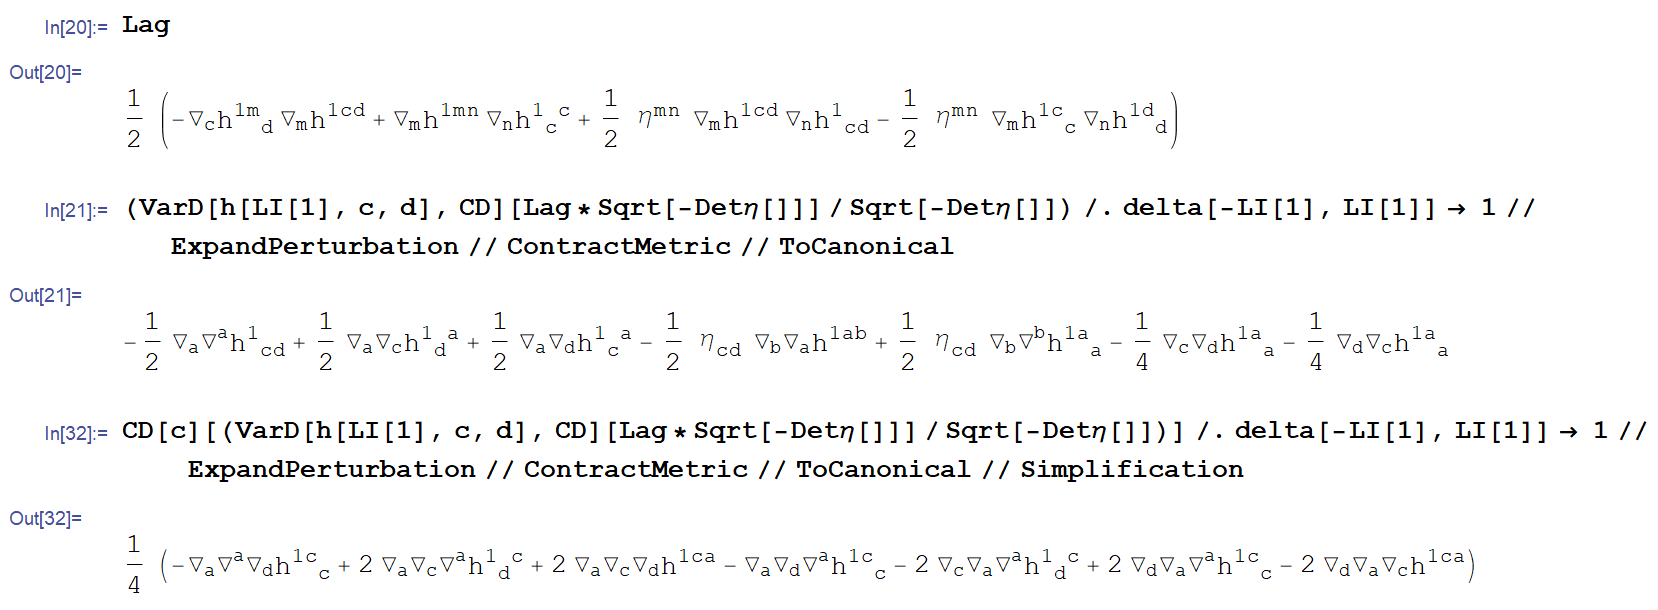
\includegraphics[scale=0.25]{CDG}
\end{figure}
So yes $\p^\mu G_{\mu\nu}$ is in fact identically zero. Thus, we must have that
\begin{align}\label{gauge-1}
\p^\mu \lc \f{1}{2}m^2 \lp h_{\mu\nu} - (1-a)\eta_{\mu\nu}h \rp \rc= 0 &\iff \boxed{\p^\mu h_{\mu\nu} - (1-a)\eta_{\mu\nu}\p^\mu h = 0}
\end{align}
Next, just like how we can write 
\begin{align}
A_\mu \sim \xi_\mu e^{ik\cdot x}
\end{align}
for the wave solution to the spin-1 field where $\xi_\mu$ is the polarization \textit{vector}, let us write
\begin{align}
h_{\mu\nu} \sim \xi_{\mu\nu}e^{ik\cdot x}
\end{align}
where $\xi_{\mu\nu}$ is the graviton's polarization tensor. With this we have
\begin{align}
\boxed{\xi_{\mu\nu}k^\mu - (1-a)\tensor{\xi}{^\mu_\mu}k_\nu = 0}
\end{align}
This is four equations for $\nu = 0,1,2,3$ which brings the number of degrees of freedom down from 10 to $10 - 4 = 6$ degrees of freedom. There is now one too many. How do we get rid of this? The answer lies in the factor $(1-a)$ and the contraction of $G^{\mu\nu}$.\\

Recall from \eqref{GGG} that
\begin{align}
G_{\mu\nu} = \f{1}{2}\lp -\square h_{\mu\nu} + \p_\sigma \p_\nu \tensor{h}{^\sigma_\mu}  
+ \p_\sigma \p_\mu \tensor{h}{^\sigma_\nu} 
- \eta_{\mu\nu}\p_\lambda \p_\sigma h^{\lambda\sigma} + \eta_{\mu\nu}\square h - \p_\mu\p_\nu h\rp,
\end{align}
which we have found by varying $\lag_{\text{linear}}$ in xACT with respect to $h_{\mu\nu}$. We wish to contract $G_{\mu\nu}$, with xACT as well:
\begin{lstlisting}
Lag := (1/
2)*((CD[-m][h[LI[1], m, n]])*(CD[-n][h[LI[1], -c, c]]) - (CD[-m][
h[LI[1], c, d]])*(CD[-c][h[LI[1], m, -d]]) + (1/2)*\[Eta][m, 
n]*(CD[-m][h[LI[1], c, d]])*(CD[-n][h[LI[1], -c, -d]]) - (1/
2)*\[Eta][m, 
n]*(CD[-m][h[LI[1], c, -c]])*(CD[-n][h[LI[1], d, -d]]))

(VarD[h[LI[1], c, d], CD][Lag*Sqrt[-Det\[Eta][]]]/
Sqrt[-Det\[Eta][]]) /. delta[-LI[1], LI[1]] -> 1 // 
ExpandPerturbation // ContractMetric // ToCanonical

\[Eta][c, 
d] (VarD[h[LI[1], c, d], CD][Lag*Sqrt[-Det\[Eta][]]]/
Sqrt[-Det\[Eta][]]) /. delta[-LI[1], LI[1]] -> 1 // 
ExpandPerturbation // ContractMetric // ToCanonical
\end{lstlisting}
\begin{figure}[!htb]
	\centering
	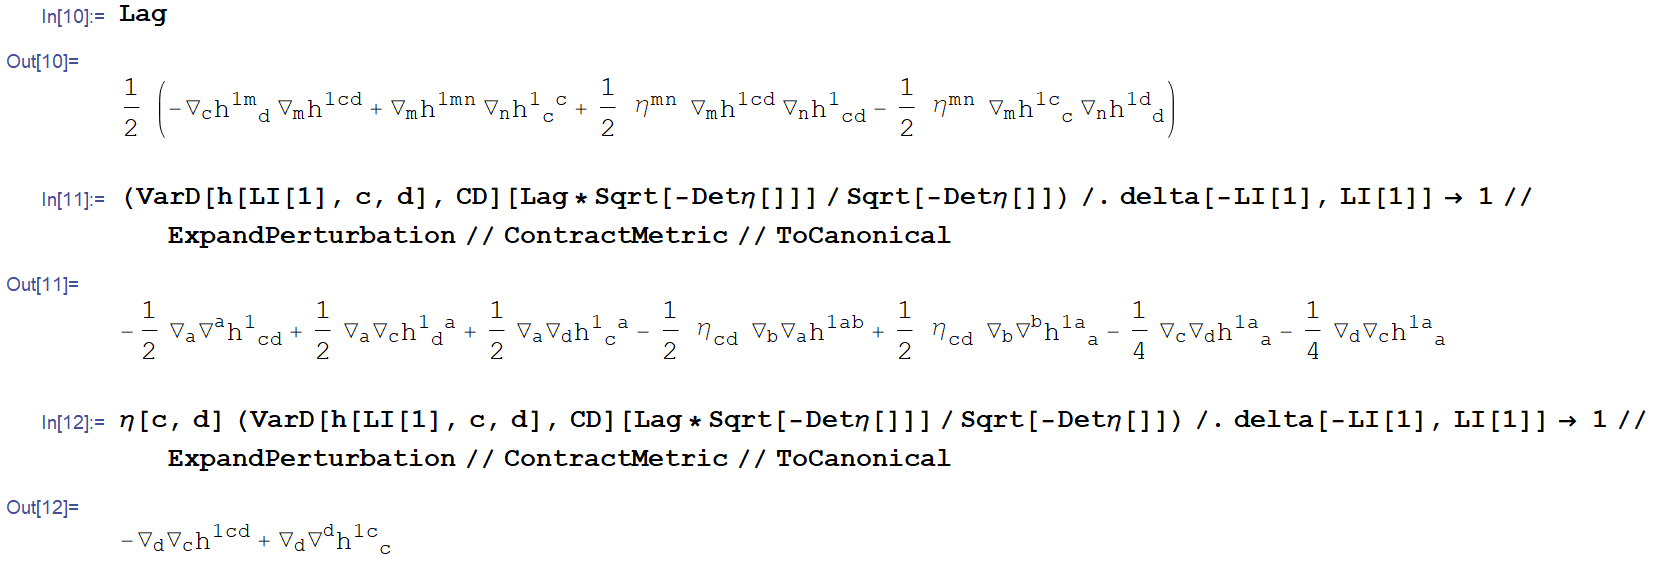
\includegraphics[scale=0.28]{Gcontract}
\end{figure}

This reads nicely as
\begin{align}\label{munuG}
\boxed{G=  \eta^{\mu\nu}G_{\mu\nu} = \p_\mu \p_\nu h^{\mu\nu} - \square h}
\end{align}
From the gauge fix in \eqref{gauge-fix}, we must have that
\begin{align}\label{munuH}
G = \eta^{\mu\nu}G_{\mu\nu} &= -\f{1}{2}m^2\eta^{\mu\nu}[ h_{\mu\nu} -(1-a)\eta_{\mu\nu}h ]\nn\\
&= -\f{1}{2}m^2 [h - 4(1-a)h]\nn\\
&= \boxed{\f{1}{2}m^2 (3 - 4a)h}
\end{align}
If we choose $a = 0$, then it follows from this equality that
\begin{align}
G =\f{1}{2}m^2h 
\end{align}
and from \eqref{gauge-1} that   
\begin{align}
\p^\mu h_{\mu\nu} - \p_\nu h = 0 \implies \p_\mu \p_\nu h^{\mu\nu} - \square h = 0.
\end{align}
But these combined give us $h = 0 \iff \tensor{h}{^\mu_\mu} \iff \tensor{\xi}{^\mu_\mu} = 0$. Aha! With the trace of $\xi_{\mu\nu}$ being zero, the number of polarizations is now $6-1 = 5$, as desired. This choice of the Fierz-Pauli tuning is now justified.\\



















\textit{Step 2.} Here we will show that when $a\neq 0$, the theory describes a massive spin 2 \textit{and} and a ghost scalar field with
\begin{align}
m_g^2  = -\f{3-4a}{2a}m^2.
\end{align}
Let us first show the motivation for defining the ghost scalar mass in this fashion. We have that \eqref{gauge-1} reads
\begin{align}
\p^\mu h_{\mu\nu} - (1-a)\eta_{\mu\nu}\p^\mu h = 0.
\end{align}
We wish to establish a relationship between $\square h$ and $\p^\mu \p^\nu h_{\mu\nu}$ for reasons we will see later. This means we should take $\p^\nu$ of the equation above. This gives
\begin{align}
\p^\nu \p^\mu h_{\mu\nu} - (1-a)\eta_{\mu\nu}\p^\nu \p^\mu h = 0.
\end{align}
But this equation simply screams
\begin{align}\label{just-then}
\p_\mu \p_\nu h^{\mu\nu} - (1-a)\square h = 0.
\end{align}

Nice! Now, from \eqref{munuG} and \eqref{munuH} we also know that
\begin{align}\label{just-now}
\p_\mu \p_\nu h^{\mu\nu} - \square h = -\f{1}{2}m^2(3-4a)h.
\end{align}
Therefore, we have from \eqref{just-now} and \eqref{just-then}
\begin{align}
-\f{1}{2}m^2 (3-4a) h + \square h = (1-a)\square h.
\end{align}
This simplifies to
\begin{align}
-\f{1}{2}m^2 (3-4a) h = -a\square h.
\end{align}
This equation is now begging to be put into Klein-Gordon form:
\begin{align}
\boxed{\lp -\f{1}{2a}m^2(3-4a) + \square \rp h = 0}
\end{align}
It only makes sense that we cast the mass term as $m_g^2$. And whatever this theory is, it is describing a massive scalar field with
\begin{align}
\boxed{m_g^2 = -\f{3-4a}{2a}m^2 }
\end{align}
Our next task is to show this is actually a ghost field. To this end, we invoke Hamiltonian analysis of Fierz-Pauli massive gravity with the $(1-a)$ coefficient. We first cast the Lagrangian 
\begin{align}
\lag = &-\f{1}{2}\p_\lambda h_{\mu\nu} \p^\lambda h^{\mu\nu} + \p_\mu h_{\nu\lambda}\p^\nu h^{\mu\lambda}\nn\\& - \p_\mu h^{\mu\nu}\p_\nu h + \f{1}{2}\p_\lambda h \p^\lambda h -\f{1}{2}m^2\lp h_{\mu\nu}h^{\mu\nu} - h^2 \rp
\end{align}
into Hamiltonian form. We start by Legendre transforming this Lagrangian only with respect to the spatial components of the perturbation metric, $h_{ij}$. The canonical momenta are defined as
\begin{align}
\pi_{ij} = \f{\p \lag}{\p \dot{h}_{ij}} \equiv \f{\p \lag}{\p (\p_0 h_{ij})}
\end{align}
where $\p$ is just the regular partial derivative. To evaluate this, we can expand out $\lag$ in terms of $\mu =0$ objects and $\mu = i = 1,2,3$ objects. If \href{https://digitalcommons.colby.edu/cgi/viewcontent.cgi?article=1721&context=honorstheses}{\underline{Greg Seyfarth}} is correct, then (deep breath now):
\begin{empheq}[box=\widefbox]{align*}
\lag = &\f{1}{2}(h_{jk,0})^2 + (h_{0k,j})^2 - \f{1}{2}(h_{jk,l})^2 - (h_{0k,j})(h_{0j,k}) - 2(h_{0j,k})(h_{jk,0})\nn\\
&+ (h_{kj,l})(h_{lj,k}) + (h_{0k,k})(h_{jj,0}) - \f{1}{2}(h_{jj,0})(h_{kk,0}) - (h_{00,l})(h_{jj,l})  \nn\\
&+\f{1}{2}(h_{jj,l})(h_{kk,l}) + (h_{0j,j})(h_{kk,0}) + (h_{jk,j})(h_{00,k}) - (h_{jk,j})(h_{ll,k}) \nn\\
& - \f{1}{2}m^2 \lb a h^2_{00} - 2h_{0j}^2 + h^2_{jk} + 2(1-a)h_{00}h_{ll} - (1-a)h^2_{ll} \rb.
\end{empheq}
To get these square terms in the Lagrangian it is necessary to integrate by parts and cancel like terms. I will not try to reproduce this since it is purely index manipulation.\\

Varying this Lagrangian gives equations of motions. Varying with respect to $h_{00}$ gives
\begin{align}
h_{jj,kk} - h_{jk,jk} - am^2h_{00} - m^2(1-a)h_{ll} - 0.
\end{align}
Varying with respect to $h_{0j}$ gives
\begin{align}
-h_{0j,kk} + h_{0k,jk} + h_{jk,0k} - h_{kk,0j} + m^2 h_{0j} = 0.
\end{align}
Varying with respect to $h_{jk}$ gives
\begin{align}
0= &\,\,\,h_{jk,00} - h_{jk,ll} - (h_{0j,0k} + h_{0k,0j}) + (h_{lk,lj} + h_{lj,lk})\nn\\
&\,\,\, + \delta_{jk}(2h_{0l,0l} - h_{ll,00} - h_{00,ll} + h_{mm,ll}- h_{lm,lm})\nn\\
&\,\,\,+ h_{00,jk} - h_{ll,jk} + m^2 h_{jk} + m^2(1-a)\delta_{jk}h_{00} - m^2(1-a)\delta_{jk}h_{ll}. 
\end{align}
With this, the Hamiltonian is
\begin{empheq}[box=\widefbox]{align*}
\ham &= \pi^{\mu\nu} h_{\mu\nu,0} - \lag \nn\\
&= \f{1}{2}(\pi_{jk})^2 - \f{1}{4}(\pi_{ll})^2 + 2 h_{0k,j}\pi_{jk} + \f{1}{2}(h_{jk,l})^2\nn\\
&\,\,\,\, -h_{jk,l}h_{lj,k} + h_{00,l}h_{kk,l} - \f{1}{2}h_{jj,l}h_{kk,l} - h_{jk,j}h_{00,k}+ h_{jk,j}h_{ll,k}\nn\\
&\,\,\,\, + \f{1}{2}m^2[ah^2_{00} - 2h^2_{0j} + h^2_{jk} + 2(1-a)h_{00}h_{ll}h - (1-a)h^2_{ll}].  
\end{empheq}
After a number of substitutions that I won't worry about too much here, the final form of the Hamiltonian is given by
\begin{empheq}[box=\widefbox]{align*}
\ham = &\f{1}{2}(\pi_{jk})^2 - \f{1}{4}(\pi_{ll})^2 + \f{1}{2}(\epsilon_{ijk} h_{kl,j})^2 -\f{1}{2}h_{jk,k}^2 + \f{1}{2}h^2_{jj,l} \nn\\
&\,\,\, + \f{1}{2}m^2[-ah^2 + h^2_{ll} + 2h_{0j}^2 + h^2_{jk}]
\end{empheq}
where $\epsilon_{ijk}$ is the Levi-Civita symbol.\\


The terms in the square brackets correspond to the Fierz-Pauli mass term in the original Lagrangian, while the rest of the terms come from the Lagrangian that gives the original Einstein tensor. We are interested in the square bracket terms when looking for ghosts in the theory. \\

When $a=0$, the square bracket becomes
\begin{align}
\f{1}{2}m^2[-ah^2 + h^2_{ll} + 2h_{0j}^2 + h^2_{jk}] \to \f{1}{2}m^2[h^2_{ll} + 2h_{0j}^2 + h^2_{jk}].
\end{align}
This term is positive-definite, which is good. But what about the other terms in the Hamiltonian? Well, we know that the rest of the Hamiltonian comes directly from the Lagrangian without the massive term. We also know that this piece of the theory is very well-behaved since we have a number of equations of motions and constraints to keep the degree of freedom correct. Thus, to see if the current theory contains ghost it suffices to look only at the massive term's contribution to the Hamiltonian. \\

Since we have already seen how $a= 0$ gives a well-behaved theory. Let's now consider $a\neq 0$. When $a\neq 0$, the modified Klein-Gordon equation looks like
\begin{align}
\lp -\f{3-4a}{2a}m^2 + \square\rp h = (\square + m_g^2)h = 0. 
\end{align}
Clearly the energy relation is 
\begin{align}
E^2 - p^2 = -m_g^2,
\end{align}
which has the wrong sign, i.e., the (ghostly) mass is imaginary. We might try to remedy this problem by requiring that
\begin{align}
\f{3-4a}{2a} > 0 \iff 0 < a < \f{3}{4}.
\end{align}
But this ensures that the coefficient of $h^2$ in the term
\begin{align}
\f{1}{2}m^2[-ah^2 + h^2_{ll} + 2h_{0j}^2 + h^2_{jk}]
\end{align}
is always negative, rendering the Hamiltonian non-positive-definite. We also can't constrain $h$ in order to bring the degree of freedom down from 6 to 5. This means that when $a\neq 0$ we have (1) an imaginary mass, (2) non-positive definite Hamiltonian, and (3) and extra degree of freedom in the theory. This creates a ghost mode in the theory.\\ \qed

With that we have showed how the tuning $a = 0$ is justified, and how a massive scalar ghost mode appears (with negative kinetic energy) in the theory when $a \neq 0$. As a little aside, when $a\neq0$ and $a$ is small, the mass $m_g^2$ goes like $\sim 1/a$. This goes to infinity as the Fierz-Pauli tuning is approached, rendering it non-dynamical.


























\subsubsection{Free solutions and Graviton mode functions}

In this section we find the space of equations of motion, i.e. solutions to $\delta S = 0$. We will then show that it transforms as a massive spin 2 representation of the Lorentz group, i.e. showing that the action propagates precisely one massive graviton (we will understand what this means later). To this end, we consider the Fierz-Pauli action with the correct Fierz-Pauli tuning:
\begin{align}
S_{FP} = \int d^Dx\, &-\f{1}{2}\p_\lambda h_{\mu\nu} \p^\lambda h^{\mu\nu} + \p_\mu h_{\nu\lambda}\p^\nu h^{\mu\lambda}\nn\\& - \p_\mu h^{\mu\nu}\p_\nu h + \f{1}{2}\p_\lambda h \p^\lambda h -\f{1}{2}m^2\lp h_{\mu\nu}h^{\mu\nu} - h^2 \rp.
\end{align}  
Setting $\delta S = 0 \iff \delta \lag / \delta h^{\mu\nu} = 0$, i.e., the variational derivative of the integrand with respect to the inverse metric perturbation $h^{\mu\nu}$ is zero. We can readily to this in xACT:
\begin{lstlisting}
LagFP := -((CD[-m][h[LI[1], m, n]])*(CD[-n][
h[LI[1], -c, c]]) - (CD[-m][h[LI[1], c, d]])*(CD[-c][
h[LI[1], m, -d]]) + (1/2)*\[Eta][m, 
n]*(CD[-m][h[LI[1], c, d]])*(CD[-n][h[LI[1], -c, -d]]) - (1/
2)*\[Eta][m, 
n]*(CD[-m][h[LI[1], c, -c]])*(CD[-n][h[LI[1], d, -d]])) - (1/
2)*M^2*(h[LI[1], m, n]*
h[LI[1], -m, -n] - (1 - 0) h[LI[1], c, -c]*h[LI[1], d, -d])

(VarD[h[LI[1], c, d], CD][LagFP*Sqrt[-Det\[Eta][]]]/
Sqrt[-Det\[Eta][]]) == 0 /. delta[-LI[1], LI[1]] -> 1 // 
ExpandPerturbation // ContractMetric // ToCanonical
\end{lstlisting}
to get
\begin{figure}[!htb]
	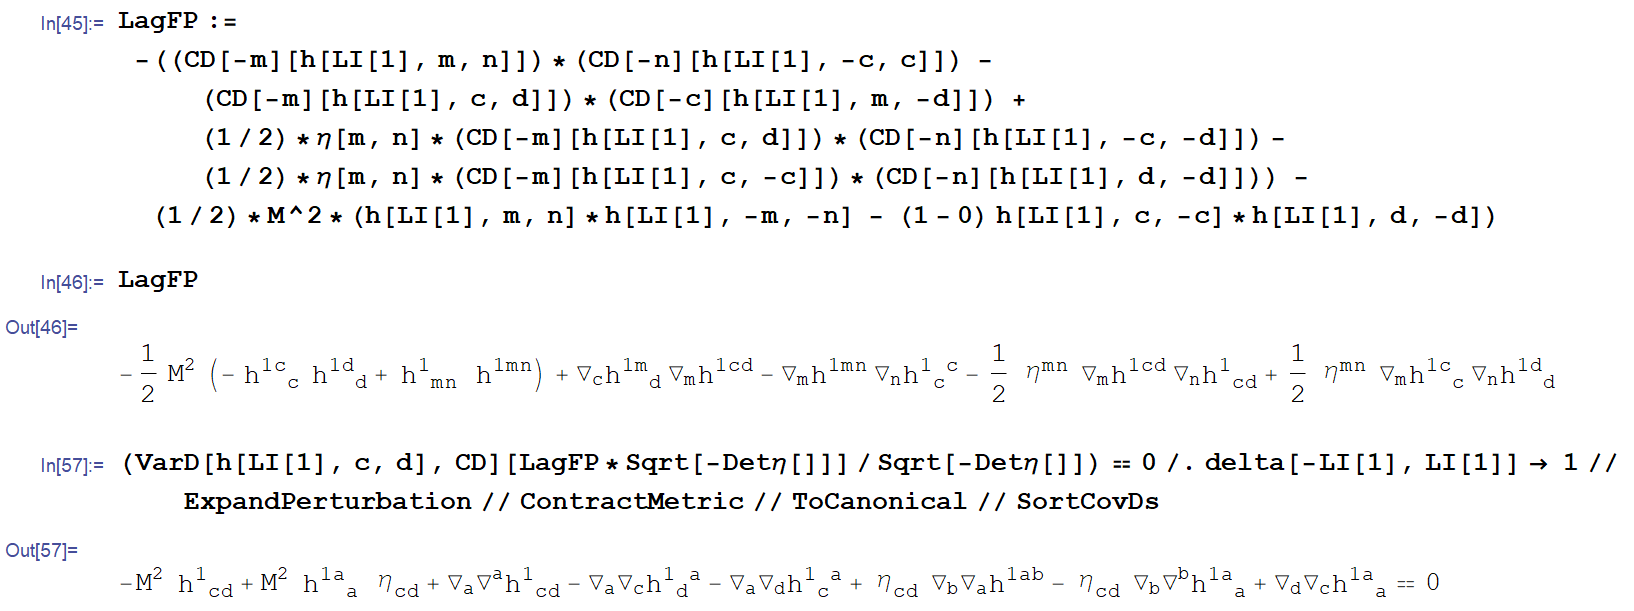
\includegraphics[scale=0.26]{free-soln}
\end{figure}\\
which says
\begin{align}
\f{\delta \lag}{\delta h^{\mu\nu}} &= \square h_{\mu\nu} - \p_\lambda \p_\mu \tensor{h}{^\lambda_\nu} - \p_\lambda \p_\nu \tensor{h}{^\lambda_\mu} + \eta_{\mu\nu}\p_\lambda \p_\sigma h^{\lambda\sigma} + \p_\mu \p_\nu h - \eta_{\mu\nu}\square h  \nn\\
&\,\,\,\,\,- m^2(h_{\mu\nu} - \eta_{\mu\nu}h)\nn\\
&= 0.
\end{align}

Okay, to get what constraints this equation gives us we first let $\p^\mu$ act on this equation:
\begin{lstlisting}
CD[c][(VarD[h[LI[1], c, d], CD][LagFP*Sqrt[-Det\[Eta][]]]/
Sqrt[-Det\[Eta][]])] /. delta[-LI[1], LI[1]] -> 1 // 
ExpandPerturbation // ContractMetric // 
ToCanonical // Simplification
\end{lstlisting}
\begin{figure}[!htb]
	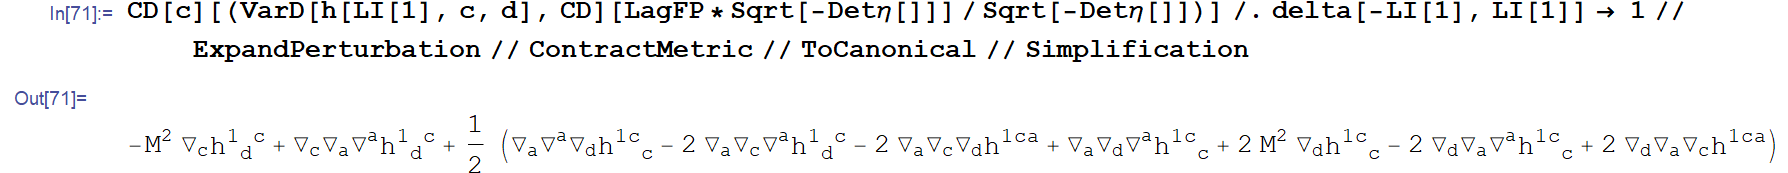
\includegraphics[scale=0.26]{covD}
\end{figure}
Looking at this expression (which equals 0) for a while we can see that all terms without the $m^2$ factor cancel, which makes sense because $\p^\mu G_{\mu\nu} = 0$ where $G^{\mu\nu}$ is the Einstein tensor in the massless case. This expression then just simplify to
\begin{align}
\boxed{\p^\mu h_{\mu\nu} - \p_\nu h = 0 \iff \p_\mu h^{\mu\nu} - \p^\nu h = 0}
\end{align}
Plugging this back into the equation of motion, we find
\begin{align}
0 &= \square h_{\mu\nu} - \p_\lambda \p_\mu \tensor{h}{^\lambda_\nu} - \p_\lambda \p_\nu \tensor{h}{^\lambda_\mu} + \eta_{\mu\nu}\p_\lambda \p_\sigma h^{\lambda\sigma} + \p_\mu \p_\nu h - \eta_{\mu\nu}\square h - m^2(h_{\mu\nu} - \eta_{\mu\nu}h)\nn\\
&= \square h_{\mu\nu} - \p_\mu \p^\lambda h_{\lambda\nu} - \p_\nu \p^\lambda h_{\lambda\mu} + \eta_{\mu\nu}\p_\lambda \p^\lambda h + \p_\mu \p_\nu h - \eta_{\mu\nu}\square h - m^2(h_{\mu\nu} - \eta_{\mu\nu}h)\nn\\
&= \square h_{\mu\nu} - \p_\mu \p_\nu h - \p_\nu \p_\mu h + \cancel{\eta_{\mu\nu}\square h} + \p_\mu \p_\nu h - \cancel{\eta_{\mu\nu}\square h} - m^2(h_{\mu\nu} - \eta_{\mu\nu}h)\nn\\
&= \square h_{\mu\nu} - \p_\mu \p_\nu h - m^2(h_{\mu\nu} - \eta_{\mu\nu}h).
\end{align}
So we have
\begin{align}
\boxed{\square h_{\mu\nu} - \p_\mu \p_\nu h - m^2(h_{\mu\nu} - \eta_{\mu\nu}h) = 0}
\end{align}
Contracting we find that $\boxed{h=0}$
\begin{align}
0 &= \eta^{\mu\nu}\lp \square h_{\mu\nu} - \p_\mu \p_\nu h - m^2(h_{\mu\nu} - \eta_{\mu\nu}h) \rp\nn\\
&= \square h - \square h - m^2(h - 4h) \iff h = 0.
\end{align}
But this just says
\begin{align}
\p^\mu h_{\mu\nu} = \p_\nu h = 0 \implies (\square - m^2)h_{\mu\nu} = 0.
\end{align}
And so just to summarize, we have
\begin{align}
\boxed{(\square - m^2)h_{\mu\nu} = 0; \quad \p^\mu h_{\mu\nu} = 0; \quad h = 0}
\end{align}
It turns out that these three equations and the original equation of motion $\delta \lag = 0$ are equivalent statements. However, when put into this form (involving three simple equations), degree-of-freedom-counting is much easier. For $D = 4$, the first equation describe the evolution for a ten-component symmetric tensor $h$. The second equation reduces 4 more d.o.f. The last equation sets the trace, hence killing the last d.o.f, making $h_{\mu\nu}$ have only 5 d.o.f. In total, we are left with the 5 real space d.o.f of a 4-dimensional spin 2 particle ($5 = 2s+1 = 2\times 2 + 1$). \\

Next, we wish to solve for $h_{\mu\nu}$ firstly from the Klein-Gordon equation. This turns out to be a reasonably easy differential equation whose general solution has the form
\begin{align}
\boxed{h^{\mu\nu}(x) = \int \f{d^d\mathbf{p}}{\sqrt{(2\pi)^d 2\omega_\mathbf{p}}} \lb h^{\mu\nu}(\mathbf{p})e^{ip\cdot x} + {h^{\mu\nu}}^*(\mathbf{p})e^{-ip\cdot x}\rb}
\end{align}  
Here $\mathbf{p}$ are the spatial momenta:
\begin{align}
\omega_\mathbf{p} = \sqrt{\mathbf{p}^2 +m^2},
\end{align}
and the $D$ momenta $p^\mu$ are on shell so that $p^\mu =(\omega_\mathbf{p}, \mathbf{p})$. We then express the Fourier coefficients $h^{\mu\nu}(\mathbf{p})$ in terms of basis symmetric tensors indexed by $\lambda$:
\begin{align}
h^{\mu\nu}(\mathbf{p}) = a_{\mathbf{p},\lambda}\bar{\mathbf{\epsilon}}^{\mu\nu}(\mathbf{p},\lambda)
\end{align}
where
\begin{align}
\bar{\mathbf{\epsilon}}^{\mu\nu}(\mathbf{p},\lambda) = L^\mu_\alpha(p)L^\nu_\beta(p)\bar{\mathbf{\epsilon}}^{\alpha\beta}(\mathbf{k},\lambda).
\end{align}
Here $L^\mu_\alpha(p)$ are boosts of the form
\begin{align}
&L^i_j(p) = \delta^i_j + \f{1}{\abs{\mathbf{p}}^2}(\gamma - 1)\mathbf{p}^i\mathbf{p}^j\nn\\
&L^i_0(p) = L^0_i(\mathbf{p}) = \f{\mathbf{p}^i}{\abs{\mathbf{p}}}\sqrt{\gamma^2 - 1}\nn\\
&L^0_0(p) = \gamma = \f{p^0}{m}  = \sqrt{\abs{p}^2 + \f{m^2}{m}}
\end{align}
such that the momentum $k$ is taken from $k^\mu = (m,0,0,0)$ to $p$ where $p^\mu = L^\mu_\alpha(p) k^\alpha$. This stand boost choose for us the basis at $\mathbf{p}$, relative to that at $\mathbf{k}$. \\

With $\p_\mu h^{\mu\nu} = (\p/\p x^\mu)h^{\mu\nu}  = 0$ we have
\begin{align}
0 &= \p_\mu \lc \int \f{d^d\mathbf{p}}{\sqrt{(2\pi)^d 2\omega_\mathbf{p}}} \lb h^{\mu\nu}(\mathbf{p})e^{ip\cdot x} + {h^{\mu\nu}}^*(\mathbf{p})e^{-ip\cdot x}\rb  \rc\nn\\
&= \int \f{d^d\mathbf{p}}{\sqrt{(2\pi)^d 2\omega_\mathbf{p}}}
\lb ip_\mu  h^{\mu\nu}(\mathbf{p})e^{ip_\mu x^\mu} + h.c. \rb\nn\\
&\implies p_\mu h^{\mu\nu}(\mathbf{p}) = 0\nn\\
&\implies L^\sigma_\mu(p)k_\sigma \lp a_{\mathbf{p},\lambda}\bar{\mathbf{\epsilon}}^{\mu\nu}(\mathbf{p},\lambda)\rp = 0\nn\\
&\implies k_\sigma L^\sigma_\mu(p)L^\mu_\alpha(p)L^\nu_\beta(p)\bar{\mathbf{\epsilon}}^{\alpha\beta}(\mathbf{k},\lambda) =0 \nn\\
&\implies k_\sigma \delta^\sigma_\alpha(p)L^\nu_\beta(p)\bar{\mathbf{\epsilon}}^{\alpha\beta}(\mathbf{k},\lambda) =0 \nn\\
&\implies k_\alpha L^\nu_\beta(p)\bar{\mathbf{\epsilon}}^{\alpha\beta}(\mathbf{k},\lambda) =0 \nn\\
&\implies k_\alpha\bar{\mathbf{\epsilon}}^{\alpha\beta}(\mathbf{k},\lambda) =0 \nn\\
&\implies \boxed{k_\mu \bar{\mathbf{\epsilon}}^{\mu\nu}(\mathbf{k},\lambda) = 0  }
\end{align} 
We also have the condition $h=0$, which implies
\begin{align}
0 &= \eta_{\mu\nu}\int \f{d^d\mathbf{p}}{\sqrt{(2\pi)^d 2\omega_\mathbf{p}}} \lb h^{\mu\nu}(\mathbf{p})e^{ip\cdot x} + {h^{\mu\nu}}^*(\mathbf{p})e^{-ip\cdot x}\rb\nn\\
&\implies \eta_{\mu\nu}a_{\mathbf{p},\lambda}\bar{\mathbf{\epsilon}}^{\mu\nu}(\mathbf{p},\lambda) = 0\nn\\
&\implies \eta_{\mu\nu}a_{\mathbf{p},\lambda}L^\mu_\alpha(p)L^\nu_\beta(p)\bar{\mathbf{\epsilon}}^{\alpha\beta}(\mathbf{k},\lambda) = 0\nn\\
&\implies \dots (\text{requires writing out when $\alpha=\mu$, $\beta=\nu$, etc.})\nn\\
&\implies \boxed{\eta_{\mu\nu}\bar{\mathbf{\epsilon}}^{\mu\nu}(\mathbf{k},\lambda) = 0}
\end{align}
These two conditions imply that $\bar{\mathbf{\epsilon}}^{\mu\nu}(\mathbf{k},\lambda)$ is purely spatial, i.e.
\begin{align}
\boxed{\bar{\epsilon}^{0\mu}(\mathbf{k},\lambda) = \bar{\epsilon}^{0\mu}(\mathbf{k},\lambda)   = 0}
\end{align}
i.e.,
\begin{align}
[\bar{\mathbf{\epsilon}}^{\mu\nu}] = \begin{pmatrix}
0 &0&0&0\\
0&\bar{\mathbf{\epsilon}}^{11}&\bar{\mathbf{\epsilon}}^{12}&\bar{\mathbf{\epsilon}}^{13}\\
0&\bar{\mathbf{\epsilon}}^{12}&\bar{\mathbf{\epsilon}}^{22}&\bar{\mathbf{\epsilon}}^{23}\\
0&\bar{\mathbf{\epsilon}}^{13}&\bar{\mathbf{\epsilon}}^{23}&\bar{\mathbf{\epsilon}}^{33}\\
\end{pmatrix}
\end{align}
and that $\bar{\mathbf{\epsilon}}^{\mu\nu}(\mathbf{k},\lambda)$ is traceless, i.e.,
\begin{align}
\boxed{\bar{\mathbf{\epsilon}}^i_i(\mathbf{k},\lambda) = 0}
\end{align}
Hence, this basis is a collection of $d(d+1)/2$ symmetric, traceless spatial tensors with index $\lambda = 1,\dots,d(d+1)/2$. \\

We demand further that this is an orthonormal basis:
\begin{align}
\boxed{\bar{\mathbf{\epsilon}}^{\mu\nu}(\mathbf{k},\lambda)\bar{\mathbf{\epsilon}}^*_{\mu\nu}(\mathbf{k},\lambda') = \delta_{\lambda\lambda'}}
\end{align}


\textit{(some things about group theory here... in order to make conditions work for $\mathbf{p}$ and not $\mathbf{k}$..., i.e.,}
\begin{align}
\boxed{p_\mu \mathbf{\epsilon}^{\mu\nu}(\mathbf{p},\lambda) = 0; \quad \eta_{\mu\nu}\mathbf{\epsilon}^{\mu\nu}(\mathbf{p},\lambda) = 0}
\end{align}

\textit{I will get back to this later)}\\

In any case, the general solution $h^{\mu\nu}(x)$ can now be written in term of the new $\mathbf{p}$-dependent basis:
\begin{align}
h^{\mu\nu}(x) = \int \f{d^d\mathbf{p}}{\sqrt{(2\pi)^d 2\omega_\mathbf{p}}} \sum_\lambda a_{\mathbf{p},\lambda} \mathbf{\epsilon}^{\mu\nu}(\mathbf{p},\lambda)e^{ip\cdot x} + a^*_{\mathbf{p},\lambda} \mathbf{\epsilon}^{*\mu\nu}(\mathbf{p},\lambda)e^{-ip\cdot x}
\end{align}
























\subsubsection{The Propagator}

There is a treatment of the F-P propagator in A. Zee's book which I have reproduced in one of sections in \textit{Gravity as Field Theory}. But in any case, I will reproduce the derivation here (plus some details) following Hinterbichler's paper. \\

The recall the full Fierz-Pauli action:
\begin{empheq}[box=\widefbox]{align}
S_{FP} = \int d^Dx\, &-\f{1}{2}\p_\lambda h_{\mu\nu} \p^\lambda h^{\mu\nu} + \p_\mu h_{\nu\lambda}\p^\nu h^{\mu\lambda}\nn\\& - \p_\mu h^{\mu\nu}\p_\nu h + \f{1}{2}\p_\lambda h \p^\lambda h -\f{1}{2}m^2\lp h_{\mu\nu}h^{\mu\nu} - h^2 \rp
\end{empheq}
We wish to write this action in the form
\begin{align}
S = \int d^Dx\,\f{1}{2}h_{\mu\nu}\mathcal{O}^{\mu\nu,\alpha\beta}h_{\alpha\beta}
\end{align}
so as to resemble quantum field theory where the action appearing in the generating function 
\begin{align}
\Z = \zeta \int \mathfrak{D}[\phi] e^{i\int d^4x \lag[\phi]}\sim e^{\f{-i}{2}JA^{-1}J} \equiv e^{\f{-i}{2}\iint d^4xd^4y J(x)\D(x-y)J(y)}
\end{align}
where $J(\cdot)$ is the source and $\D(x-y) \equiv A^{-1}$ is the propagator and $A$ is the original differential operator in the Lagrangian. By analogy, the graviton propagator $\D_{\alpha\beta,\mu\nu}$ is defined to be the inverse of the second-order differential operator $\mathcal{O}^{\mu\nu,\alpha\beta}$. The goal of this section is to obtain an expression for $\D_{\alpha\beta,\mu\nu}$.\\

We wish to turn $S_{FP}$ into the form involving $\mathcal{O}^{\mu\nu,\alpha\beta}$ where $\mathcal{O}^{\mu\nu,\alpha\beta}$ is some operator. The comma here doesn't mean (covariant) derivatives of any kind. It is there just to remind us that $\mu\nu$ and $\alpha\beta$ can be treated as two (pair of) indices. To write the action this way we are required to integrate the integrand of $S_{FP}$ by parts so that every term in the resulting integrand looks like $h_{\mu\nu}\diamondsuit^{\mu\nu,\alpha\beta}h_{\alpha\beta}$ where $\diamondsuit^{\mu\nu,\alpha\beta}$ is some operator. There are five terms so let's hope things don't get out of hand (they don't). The first term can be re-written as
\begin{align}
\int d^Dx\, \f{1}{2} \lp -\p_\lambda h_{\mu\nu}\p^\lambda h^{\mu\nu} \rp 
&= \int d^Dx\, \f{1}{2}\lp h_{\mu\nu} \square \eta^{\mu\alpha}\eta^{\nu\beta}h_{\alpha\beta} \rp\nn\\
&= \int d^Dx\, \f{1}{2}\lp h_{\mu\nu} \square \tensor{\eta}{^{(\mu}_\alpha}\tensor{\eta}{^{\nu)}_{\beta}}h^{\alpha\beta} \rp
\end{align}
where the little brackets denote the symmetry in $\mu \leftrightarrow \nu$, meaning that we can swap $\mu$ and $\nu$ as we please. \\

The second term is the trickiest:
\begin{align}
\int d^Dx\, \lp\p_\mu h_{\nu\lambda}\p^\nu h^{\mu\lambda}\rp &= \int d^Dx\, \lp - h_{\nu\lambda}\p_\mu \p^\nu h^{\mu\lambda}\rp \nn\\
&= \int d^Dx\, \lp -h_{\mu\nu}\p^\alpha \p^\mu \eta^{\nu\beta}h_{\alpha\beta} \rp\nn\\
&= \int d^Dx\, \lb h_{\mu\nu}\lp - \p^\mu \p^\alpha \eta^{\nu\beta} - \p^\nu \p^\beta \eta^{\mu\alpha} + \p^\alpha \p^\beta \eta^{\mu\nu}  \rp h_{\alpha\beta} \rb\nn\\
&= \int d^Dx\, \lb h_{\mu\nu} \lp -2\p^{(\mu} \p^{(\alpha} \tensor{\eta}{^{\nu)\beta)}} + \p^\alpha \p^\beta \eta^{\mu\nu}  \rp h_{\alpha\beta} \rb\nn\\
&= \int d^Dx\, \lb h_{\mu\nu} \lp -2\p^{(\mu} \p_{(\alpha} \tensor{\eta}{^{\nu)}_{\beta)}} + \p_\alpha \p_\beta \eta^{\mu\nu}  \rp h^{\alpha\beta} \rb,
\end{align}
where we're treating $\mu$ and $\nu$ are one pair and $\alpha$ and $\beta$ as another pair. The last three terms are quite easy:
\begin{align}
\int d^Dx\, \lp-\p_\mu h^{\mu\nu}\p_\nu h \rp 
&= \int d^Dx\, \lp h^{\mu\nu}\p_\mu\p_\nu h \rp  \nn\\
&= \int d^Dx\, \lp h_{\mu\nu}\p^\mu\p^\nu \eta^{\alpha\beta}h_{\alpha\beta} \rp  \nn\\
&= \int d^Dx\, \lp h_{\mu\nu}\p^\mu\p^\nu \eta_{\alpha\beta}h^{\alpha\beta} \rp.
\end{align}
\begin{align}
\int d^Dx\, \f{1}{2}\lp \p_\lambda h \p^\lambda h \rp
&= \int d^Dx\, \f{1}{2}\lp \p_\lambda h \p^\lambda h \rp\nn\\ 
&= \int d^Dx\, \f{1}{2}\lp -h\square h \rp\nn\\
&= \int d^Dx\, \f{1}{2}\lp -h_{\mu\nu}\square \eta^{\mu\nu}\eta^{\alpha\beta}h_{\alpha\beta} \rp\nn\\
&= \int d^Dx\, \f{1}{2}\lp -h_{\mu\nu}\square \eta^{\mu\nu}\eta_{\alpha\beta}h^{\alpha\beta} \rp.
\end{align}
\begin{align}
\int d^Dx\, -\f{m^2}{2}\lp h_{\mu\nu}h^{\mu\nu} - h^2 \rp
&= \int d^Dx\, \f{-m^2}{2}\lp h_{\mu\nu}h^{\mu\nu} - h^2 \rp\nn\\
&= \int d^Dx\, \f{-m^2}{2}\lb h_{\mu\nu}\lp\eta^{\mu\alpha}\eta^{\nu\beta}  - \eta^{\mu\nu}\eta^{\alpha\beta}\rp h_{\alpha\beta}  \rb \nn\\
&= \int d^Dx\, \f{-m^2}{2}\lb h_{\mu\nu}\lp\eta^{\mu\alpha}\eta^{\nu\beta}  - \eta^{\mu\nu}\eta^{\alpha\beta}\rp h_{\alpha\beta}  \rb \nn\\
&= \int d^Dx\, \f{-m^2}{2}\lb h_{\mu\nu}\lp\tensor{\eta}{^{(\mu}_\alpha}\tensor{\eta}{^{\nu)}_\beta}  - \eta^{\mu\nu}\eta_{\alpha\beta}\rp h^{\alpha\beta}  \rb.
\end{align}
Putting everything together we have
\begin{align}
\boxed{\tensor{\mathcal{O}}{^{\mu\nu}_{\alpha\beta}} = \lp \tensor{\eta}{^{(\mu}_\alpha}\tensor{\eta}{^{\nu)}_\beta}  - \eta^{\mu\nu}\eta_{\alpha\beta} \rp (\square - m^2) -2\p^{(\mu} \p_{(\alpha} \tensor{\eta}{^{\nu)}_{\beta)}} + \p_\alpha \p_\beta \eta^{\mu\nu} + \p^\mu\p^\nu \eta_{\alpha\beta}}
\end{align}


This operator $\mathcal{O}$ is a second order differential operator. By the symmetry in the index-pairs: $\mu\nu$ and $\alpha\beta$, we have the following property:
\begin{align}
\mathcal{O}^{\mu\nu,\alpha\beta} = \mathcal{O}^{\nu\mu,\alpha\beta} = \mathcal{O}^{\mu\nu,\beta\alpha} = \mathcal{O}^{\nu\mu,\beta\alpha}.
\end{align}
There's nothing surprising about this. It is just a fact that might be useful later. \\

With this operator, the equation of motion can now be written succinctly as
\begin{align}
\boxed{\f{\delta \lag}{\delta h_{\mu\nu}} = \mathcal{O}^{\mu\nu,\alpha\beta}h_{\alpha\beta}= 0} 
\end{align}

Recall in QFT where the propagator $\D$ is defined as the inverse of the differential operator $A$, we do the same thing here and define the propagator $\D_{\alpha\beta,\sigma\lambda}$ as the inverse of $\mathcal{O}^{\mu\nu,\alpha\beta}$:
\begin{align}
\boxed{\mathcal{O}^{\mu\nu,\alpha\beta}\D_{\alpha\beta,\sigma\lambda} = \f{i}{2}\lp \delta^\mu_\sigma \delta^\nu_\lambda + \delta^\nu_\sigma\delta^\mu_\lambda \rp}
\end{align}
which obeys the same index symmetries as $\mathcal{O}$.\\

To derive an expression for $\D$, we first write $\mathcal{O}$ in momentum space:
\begin{align}
\tensor{\mathcal{O}}{^{\mu\nu}_{\alpha\beta}}(\p \to ip) = &-\lp \tensor{\eta}{^{(\mu}_\alpha}\tensor{\eta}{^{\nu)}_\beta}  - \eta^{\mu\nu}\eta_{\alpha\beta} \rp (p^2 + m^2)\nn\\
&+2p^{(\mu} p_{(\alpha} \tensor{\eta}{^{\nu)}_{\beta)}} - p_\alpha p_\beta \eta^{\mu\nu} - p^\mu p^\nu \eta_{\alpha\beta}
\end{align}
where $\p \to ip$ denotes replacing $\p$ by $ip$ when we go to momentum space. \\

Upon inspection, we can solve for $\D$ and find
\begin{align}
\boxed{\D_{\alpha\beta,\sigma\lambda} = \f{-i}{p^2 +m^2}\lb \f{1}{2}\lp P_{\alpha\sigma}P_{\beta\lambda} + P_{\alpha\lambda}P_{\beta\sigma} \rp - \f{1}{D-1}P_{\alpha\beta}P_{\sigma\lambda} \rb}
\end{align}
where
\begin{align}
P_{\alpha\beta} = \eta_{\alpha\beta} + \f{p_\alpha p_\beta}{m^2}.
\end{align}
I won't into the details about how we can obtain this. I will just say that we can readily verify that $\D$ is indeed the inverse of the $\mathcal{O}$, in momentum space. \\

When the momentum is large, the propagator behaves as $\sim p^2 / m^4$ (rather than $1/p^2$ in the meson theory, say), and so we can't verify if the theory is renormalizable or not using the conventional power counting method. We will see later how to overcome this difficulty by rewriting the theory in a way in which all propagators go similar to $\sim 1/p^2$ at high energy.   \\

We might learn something from comparing this propagator to the propagator in the $m=0$ case. In the $m=0$ case, the action can be written as
\begin{align}
S_{m=0} = \int d^Dx\, \f{1}{2}h_{\mu\nu}\mathcal{E}^{\mu\nu,\alpha\beta}h_{\al\be}
\end{align} 
where now the differential operator $\mathcal{E}$ is just the operator $\mathcal{O}$ evaluated at $m=0$:
\begin{align}
\tensor{\mathcal{E}}{^{\mu\nu}_{\alpha\beta}} &= \tensor{\mathcal{O}}{^{\mu\nu}_{\alpha\beta}}({m=0})\nn\\
&=  \lp \tensor{\eta}{^{(\mu}_\alpha}\tensor{\eta}{^{\nu)}_\beta}  - \eta^{\mu\nu}\eta_{\alpha\beta} \rp \square -2\p^{(\mu} \p_{(\alpha} \tensor{\eta}{^{\nu)}_{\beta)}} + \p_\alpha \p_\beta \eta^{\mu\nu} + \p^\mu\p^\nu \eta_{\alpha\beta}
\end{align}
This propagator also inherits the usual index symmetry: $\mu \leftrightarrow \nu$ and $\alpha \leftrightarrow \beta$. Letting $\mathcal{E}$ act on some symmetric tensor $Z_{\alpha\beta}$ we find
\begin{align}
\mathcal{E}^{\mu\nu,\alpha\beta}Z_{\alpha\beta} &= \tensor{\mathcal{E}}{^{\mu\nu}_{\alpha\beta}}Z^{\alpha\beta}\nn\\
&= \lc\lp \tensor{\eta}{^{(\mu}_\alpha}\tensor{\eta}{^{\nu)}_\beta}  - \eta^{\mu\nu}\eta_{\alpha\beta} \rp \square -2\p^{(\mu} \p_{(\alpha} \tensor{\eta}{^{\nu)}_{\beta)}} + \p_\alpha \p_\beta \eta^{\mu\nu} + \p^\mu\p^\nu \eta_{\alpha\beta}\rc Z^{\alpha\beta}\nn\\
&= \square Z^{\mu\nu} - \eta^{\mu\nu}\square Z -2\p^{(\mu} \p_{(\alpha} \tensor{\eta}{^{\nu)}_{\beta)}}Z^{\alpha\beta} + \p^\mu\p^\nu Z + \eta^{\mu\nu}\p_\alpha\p_\beta Z^{\alpha\beta}\nn\\
&= \square Z^{\mu\nu} - \eta^{\mu\nu}\square Z -2\p^{(\mu} \p_{\alpha} \tensor{Z}{^{\nu)\alpha}} + \p^\mu\p^\nu Z + \eta^{\mu\nu}\p_\alpha\p_\beta Z^{\alpha\beta}.
\end{align}

Now, recall that the $m=0$ action has the gauge symmetry
\begin{align}
\delta h_{\mu\nu} = \p_\mu \epsilon_\nu + \p_\nu \epsilon_\mu
\end{align}
which is broken when $m\neq 0$, which implies that the operator $\mathcal{E}$ is not invertible (has non-trivial kernel, i.e. there are distinct solutions to the same problem). In order to find the propagator (of equivalently the inverse of the differential operator), we must impose a gauge. We in fact have seen this gauge before in Zee's and Sean Carroll's treatment of massive gravity. The necessary gauge condition is called the harmonic gauge or de Donder gauge or Lorenz gauge:
\begin{align}
\p^\mu h_{\mu\nu} - \f{1}{2}\p_\nu h = 0.
\end{align}   
We also know that in this gauge the equation of motion reads
\begin{align}\label{no-source}
\square h_{\mu\nu} - \f{1}{2}\eta_{\mu\nu}\square h  =0.
\end{align}
The Lagrangian associated with this gauge condition has an additive gauge-fixing term
\begin{align}
\lag_{GF} = -\lp \p^\nu h_{\mu\nu} - \f{1}{2}\p_\mu h \rp^2,
\end{align}
which we also have seen in Zee's treatment. This term actually follows from the Faddeev-Popov gauge fixing process, but I won't go into too much detail here (for reference, please refer to \textit{Gravity as a Field Theory} in one of the earlier sections). \\

When we write the gauge-fixed action as
\begin{align}
S = \int d^Dx\, (\lag + \lag_{GF}) = \int d^Dx\, \f{1}{2}h_{\mu\nu}\tilde{\mathcal{O}}^{\mu\nu,\alpha\beta}h_{\alpha\beta}
\end{align}
where, from our results in \textit{Gravity and Beyond}
\begin{align}
\lag + \lag_{GF} &= -\f{1}{2}\p_\lambda h^{\mu\nu}\p^\lambda h_{\mu\nu} +\f{1}{4} \p_\lambda \tensor{h}{^\mu_\mu} \p^\lambda \tensor{h}{^\nu_\nu} \nn\\
&= \f{1}{2}h_{\mu\nu}\square h^{\mu\nu} - \f{1}{4}h\square h
\end{align}
where some slight discrepancies in the signs of the Lagrangian here and in the earlier sections arise due to whether we vary $\lag$ with respect to  $h_{\mu\nu}$ or $h^{\mu\nu}$ (proof: a quick check in xACT). The second inequality is obtained from integrating the first line by parts (hence the minus signs). \\

With this, the new differential operator is (compare this to what we found earlier and see that they match!)
\begin{align}
\tilde{\mathcal{O}}^{\mu\nu,\alpha\beta} = \square\lb \f{\eta^{\mu\alpha}\eta^{\nu\beta} + \eta^{\mu\beta}\eta^{\nu\alpha} - \eta^{\mu\nu}\eta^{\alpha\beta}}{2}\rb
\end{align}
Going to momentum space and requiring 
\begin{align}
\tilde{\mathcal{O}}^{\mu\nu,\alpha\beta} \D_{\alpha\beta,\sigma\lambda} = \f{i}{2}\lp \delta^\mu_\sigma \delta^\nu_\lambda + \delta^\nu\sigma \delta^\mu_\lambda \rp,
\end{align}
i.e., that $\D$ is the inverse of the $\tilde{\mathcal{O}}$, we find (once again we can check with \textit{Gravity and Beyond} to see these results match up to a factor of $i$ or a minus sign due to the identity convention):
\begin{align}
\boxed{\D_{\alpha\beta,\sigma\lambda} = \f{-i}{p^2}\lb \f{1}{2}\lp \eta_{\alpha\sigma}\eta_{\beta\lambda} + \eta_{\alpha\lambda}\eta_{\beta\sigma} \rp - \f{1}{D-2}\eta_{\alpha\beta}\eta_{\sigma\lambda} \rb}
\end{align}
Notice that this propagator grows as $\sim 1/p^2$ for high energy, which is good, except this is the massless case. Comparing this result to the massive propagator, and ignoring terms that blow up when $m \to 0$, we observe a difference in the coefficient of the last term, even as $m\to 0$. When $D=4$, it is $1/2$ for the massless case and $1/3$ for the massive case:
\begin{align}
&\f{1}{D-1} \to \f{1}{4-1} = \f{1}{3}\quad \text{massive}\nn\\
&\f{1}{D-2} \to \f{1}{4-2} = \f{1}{2}\quad \text{massless}
\end{align}
This is the first hint of the vDVZ discontinuity (and various other problems that arise later).  





\newpage



\subsection{Fierz-Pauli Massive Gravity with Source}

\subsubsection{General solution to the sourced equations}

In this section we introduce a source into the action and repeat what we did in the source-free case: writing down the action, finding the equation of motion and the constraints described by it.\\


First, we add a fixed external symmetric source $T^{\mu\nu}$ to the action: 
\begin{empheq}[box=\widefbox]{align*}
S_{FP} = \int d^Dx\, &-\f{1}{2}\p_\lambda h_{\mu\nu} \p^\lambda h^{\mu\nu} + \p_\mu h_{\nu\lambda}\p^\nu h^{\mu\lambda}\nn\\& - \p_\mu h^{\mu\nu}\p_\nu h + \f{1}{2}\p_\lambda h \p^\lambda h -\f{1}{2}m^2\lp h_{\mu\nu}h^{\mu\nu} - h^2 \rp + \kappa h_{\mu\nu}T^{\mu\nu}
\end{empheq}
where
\begin{align}
\boxed{\kappa = M_P^{-(D-2)/2}}
\end{align}
is the coupling strength to the source, chosen in accord with the general relativity definition $T^{\mu\nu} = (2/\sqrt{-g})\delta L / \delta g_{\mu\nu}$ as well as the normalization $\delta g_{\mu\nu} = 2\kappa h_{\mu\nu}$.\\

The equation of motion now becomes (upon varying $\lag$ with respect to $h_{\mu\nu}$ and setting the variational derivative to zero):
\begin{align}
-\kappa T_{\mu\nu} = &\square h_{\mu\nu} - \p_\lambda \p_\mu \tensor{h}{^\lambda_\nu} -\p_\lambda \p_\nu \tensor{h}{^\lambda_\mu} + \eta_{\mu\nu}\p_\lambda\p_\sigma h^{\lambda\sigma} \nn \\ &+ \p_\mu \p_\nu h - \eta_{\mu\nu}\square h - m^2\lp h_{\mu\nu} - \eta_{\mu\nu}h \rp 
\end{align} 
When $m=0$, in which case we must have the conservation condition
\begin{align}
\p^\mu T_{\mu\nu} = 0
\end{align}
since $\p^\mu$ acting on the right-hand side when $m=0$ gives zero. When $m\neq 0$, however, $\p^\mu T_{\mu\nu} \neq 0$. In fact, letting $\p^\mu$ act on the entire equation we find the condition
\begin{align}\label{eom}
\boxed{\p^\mu h_{\mu\nu} - \p_\nu h = \f{\kappa}{m^2}\p^\mu T_{\mu\nu}}
\end{align}
whose left-hand side follows from earlier works. This is the equation of motion, whose solution can be written as a sum of a particular solution and a homogeneous solution.\\

Plugging this back into the equation of motion we find
\begin{align}
&\square h_{\mu\nu} - \p_\mu \p_\nu h - m^2\lp h_{\mu\nu} - \eta_{\mu\nu}h\rp\nn\\ = &-\kappa T_{\mu\nu} + \f{\kappa}{m^2}\lb \p^\lambda \p_\mu T_{\nu\lambda} + \p^\lambda \p_\nu T_{\mu\lambda} - \eta_{\mu\nu}\p_\mu\p_\nu T^{\mu\nu} \rb
\end{align}
Contracting this gives
\begin{align}
\square h - \square h - m^2\lp h - Dh \rp = -\kappa T + \f{\kappa}{m^2} \lb T + T - D \p_\mu\p_\nu T^{\mu\nu} \rb 
\end{align}
i.e.,
\begin{align}
\boxed{h = -\f{\kappa}{m^2(D-1)}T - \f{\kappa}{m^4}\f{D-2}{D-1}\p_\mu \p_\nu T^{\mu\nu}}
\end{align}
here $D$ is the dimension of the space we are working with. I suppose we can assume we're working in 4-dimensional spacetime, so $D$ can be set to $4$, but not necessarily. The term $\p_\mu \p_\nu T^{\mu\nu}$ can be abbreviated as $\p \p T$, denoting a double divergence. \\

Plugging this $h$ into \eqref{eom} we find
\begin{align}
\boxed{\p^\mu h_{\mu\nu} = -\f{\kappa}{m^2 (D-1)}\p_\nu T+ \f{\kappa}{m^2}\p^\mu T_{\mu\nu} - \f{\kappa}{m^4}\f{D-2}{D-1}\p_\nu \p \p T}
\end{align}
Finally, we want to know what $(\square - m^2)h_{\mu\nu}$ looks like. It turns out that (I won't go into the details here because it is relatively easy to find this):
\begin{empheq}[box=\widefbox]{align}
(\square - m^2)h_{\mu\nu}= &-\kappa \lb T_{\mu\nu} - \f{1}{D-1}\lp \eta_{\mu\nu} - \f{\p_\mu \p_\nu}{m^2}T \rp \rb\nn\\ &+ \f{\kappa}{m^2}\lb \p^\lambda \p_\mu T_{\nu\lambda} + \p^\lambda \p_\nu T_{\mu\lambda} \right. \nn\\
& \left. -\f{1}{D-1}\lp \eta_{\mu\nu} + (D-2)\f{\p_\mu \p_\nu}{m^2}\rp \p \p T \rb
\end{empheq}
These three boxed equations are the three constraints analogous to what we have found before, except here a source is present. We can also see that, just as before, these three equations combined is equivalent to the original equation of motion.\\

We can go a bit further and contract the last condition to find
\begin{align}
(\square - m^2)\underbrace{\lp h + \f{\kappa}{m^2(D-1)}T + \f{\kappa}{m^4}\f{D-2}{D-1}\p \p T \rp}_{f} = 0.
\end{align}
But of course the function $f$ here is zero because of the first condition, so there's nothing new here. However, we can look at things differently and assume that
\begin{align}
(\square - m^2)f =0\implies f =0.
\end{align}
Under this assumption the first condition is implied, and so is the second condition. With this, we may obtain solutions by Fourier transforming only the third boxed equation. Solutions can also be obtained by applying the propagator to the Fourier transform of the source (since the propagator is in momentum space).\\

We are often interested in sources that are conserved, i.e., $\p_\mu T^{\mu\nu} =0$. When the source is conserved, and under the assumption $(\square - m^2)f = 0\implies f=0$, we are left with a single equation:
\begin{align}
\boxed{(\square - m^2)h_{\mu\nu} = -\kappa \lb T_{\mu\nu} - \f{1}{D-1}\lp \eta_{\mu\nu} - \f{\p_\mu \p_\nu}{m^2} \rp T  \rb}
\end{align}
The general solution for a conserved source is then
\begin{align}\label{soln}
\boxed{h_{\mu\nu}(x) = \kappa\int \f{d^D p}{(2\pi)^D}e^{ipx}\f{1}{p^2 + m^2} \lb T_{\mu\nu}(p) - \f{1}{D-1}\lp \eta_{\mu\nu} + \f{p_\mu p_\nu}{m^2} \rp T(p) \rb}
\end{align}
where
\begin{align}
T^{\mu\nu}(p) = \int d^D x e^{-ipx}T^{\mu\nu}(x)
\end{align}
is the inverse Fourier transform of the source. 








\subsubsection{Solution for a point source ($m\neq 0$)}

We will now focus to $D=4$ so that 
\begin{align}
\kappa = M_P^{-(D-2)/2} = \f{1}{M_P}.
\end{align}
We consider as a source the stress tensor of a mass $M$ point particle at rest at the origin:
\begin{align}
\boxed{T^{\mu\nu}(x) = M \delta^\mu_0 \delta^\nu_0 \delta^3(\mathbf{x})}
\end{align} 
In momentum space this is 
\begin{align}
\boxed{T^{\mu\nu}(p) = 2\pi M \delta^\mu_0 \delta^\nu_0 \delta(p^0) \implies T(p) = \eta_{\mu\nu}T^{\mu\nu}(p) = 2\pi M \eta_{00}\delta(p^0)}
\end{align}
upon taking the Fourier transform of the $T^{\mu\nu}(x)$.\\

This source is conserved, by inspection. Using \eqref{soln}, we find (using the metric convention $\eta_{\mu\nu} = (-\,+\,+\,+)$)
\begin{align}
h_{00}(x) &= \f{1}{M_P}\int \f{d^4p}{(2\pi)^4}e^{ipx}\f{1}{p^2 + m^2}\lb T_{00}(p') - \f{1}{3}\lp \eta_{00} + \f{p_0^2}{m^2} \rp T(p') \rb\nn\\
&= \f{1}{M_P}\int \f{d^4p}{(2\pi)^4}e^{ipx}\f{1}{p^2 + m^2}\lb T_{00}(p') - \f{1}{3}\lp \eta_{00} + \f{p_0^2}{m^2} \rp \lp 2\pi M \eta_{00}\delta(p^{0'})  \rp \rb\nn\\
&= \f{M}{M_P}\int \f{d^4p}{(2\pi)^3}e^{ipx}\f{1}{p^2 + m^2}\lb \delta(p^{0'}) - \f{1}{3}\lp -1 + \underbrace{\f{p_0^2}{m^2}}_{1} \rp \delta(p^{0'}) \rb\nn\\
&= \f{2M}{3M_P}\int \f{d^4p}{(2\pi)^3}e^{ipx}\f{1}{p^2 + m^2}\delta(p^0)\nn\\
&= \f{2M}{3M_P}\int \f{d^3\mathbf{p}}{(2\pi)^3}e^{i\mathbf{p}\cdot \mathbf{x}}\f{1}{\mathbf{p}^2 + m^2}.
\end{align}
Thus we have
\begin{align}
\boxed{h_{00}(x) = \f{2M}{3M_P}\int \f{d^3\mathbf{p}}{(2\pi)^3}e^{i\mathbf{p}\cdot \mathbf{x}}\f{1}{\mathbf{p}^2 + m^2}}
\end{align}

We also have
\begin{align}
h_{0i}(x) &= \f{1}{M_P}\int \f{d^4p}{(2\pi)^4}e^{ipx}\f{1}{p^2 + m^2}\lb T_{00}(p) - \f{1}{3}\lp \eta_{0i} + \f{p_0p_i}{m^2} \rp T(p') \rb\nn\\
&= \f{1}{M_P}\int \f{d^4p}{(2\pi)^4}e^{ipx}\f{1}{p^2 + m^2}\lb T_{0i}(p) - \f{1}{3}\lp  \f{p_0p_i}{m^2} \rp \lp 2\pi M \eta_{00}\delta(p^{0'})  \rp \rb\nn\\
&= \f{1}{M_P}\int \f{d^4p}{(2\pi)^4}e^{ipx}\f{1}{p^2 + m^2}\lb 0 + 0 \rb\nn\\
&= 0
\end{align}
and so
\begin{align}
\boxed{h_{0i}(x) = 0}
\end{align}
And finally,
\begin{align}
h_{ij}(x) &= \f{1}{M_P}\int \f{d^4p}{(2\pi)^4}e^{ipx}\f{1}{p^2 + m^2}\lb T_{ij}(p) - \f{1}{3}\lp \eta_{ij} + \f{p_i p_j}{m^2} \rp T(p') \rb\nn\\
&= \f{1}{M_P}\int \f{d^4p}{(2\pi)^4}e^{ipx}\f{1}{p^2 + m^2}\lb 0 - \f{1}{3}\lp \delta_{ij} + \f{p_i p_j}{m^2} \rp \lp 2\pi M \eta_{00}\delta(p^{0'})  \rp \rb\nn\\
&= \f{M}{3M_P}\int \f{d^4p}{(2\pi)^3}e^{ipx}\f{1}{p^2 + m^2}\lb \lp \delta_{ij} + \f{p_i p_j}{m^2} \rp  \delta(p^{0'})   \rb\nn\\
&= \f{M}{3M_P}\int \f{d^3\mathbf{p}}{(2\pi)^3}e^{i\mathbf{p}\cdot \mathbf{x}}\f{1}{\mathbf{p}^2 + m^2} \lp \delta_{ij} + \f{p_i p_j}{m^2} \rp.
\end{align}
So,
\begin{align}
\boxed{h_{ij}(x) = \f{M}{3M_P}\int \f{d^3\mathbf{p}}{(2\pi)^3}e^{i\mathbf{p}\cdot \mathbf{x}}\f{1}{\mathbf{p}^2 + m^2} \lp \delta_{ij} + \f{p_i p_j}{m^2} \rp}
\end{align}


Recalling \eqref{inverse-sq} in \textit{From field to particle}, we have actually done the $h_{00}(x)$ integral. So we will just write (by analogy)
\begin{align}
{h_{00}(x) = \f{2M}{3M_P}\int \f{d^3\mathbf{p}}{(2\pi)^3}e^{i\mathbf{p}\cdot \mathbf{x}}\f{1}{\mathbf{p}^2 + m^2}= \f{2M}{3M_P}\f{1}{4\pi}\f{e^{-mr}}{r}}
\end{align}
which suggests going to spherical coordinates with $r$ being the norm of the vector $x^i$, i.e., $r = \sqrt{x_ix^i}$, integrated from $0$ to $\infty$. \\

To evaluate the $h_{ij}(x)$ integral, we can differentiate under the integral sign the integrand of $h_00(x)$ without respect to $x^i$ and $x^j$ to bring down $p_i$ and $p_j$:
\begin{align}
\p_i \p_j \lp e^{i p_\alpha x^\alpha} \f{1}{p_\beta p^\beta + m^2}\rp  =  \p_i \lb i p_j e^{i p_\alpha x^\alpha} \f{1}{p_\beta p^\beta + m^2}\rb=  -p_ip_j e^{i\mathbf{p}\cdot \mathbf{x}}\f{1}{\mathbf{p}^2 + m^2}.
\end{align} 
This, with $r = \sqrt{x_\alpha x^\alpha}$, gives
\begin{align}
\int \f{d^3\mathbf{p}}{(2\pi)^3}\f{e^{i\mathbf{p}\cdot \mathbf{x}} p_i p_j}{\mathbf{p}^2 + m^2} &= -\p_i\p_j \int \f{d^3\mathbf{p}}{(2\pi)^3}e^{i\mathbf{p}\cdot \mathbf{x}}\f{1}{\mathbf{p}^2 + m^2} \nn\\
&= -\p_i \p_j \f{1}{4\pi}\f{e^{-mr}}{r} \nn\\
&= -\p_i \p_j \f{1}{4\pi}\f{e^{-m\sqrt{x_\alpha x^\alpha}}}{\sqrt{x_\alpha x^\alpha}} = -\p_i \p_j \f{1}{4\pi}\f{e^{-m\sqrt{\eta_{\alpha\beta}x^\alpha x^\beta}}}{\sqrt{\eta_{\alpha\beta}x^\alpha x^\beta}}\nn\\
&= -\p_i \lb \f{1}{4\pi} \lp -\frac{e^{-m r} (m r+1)}{r^2} \rp \underbrace{\p_j \sqrt{\eta_{\alpha\beta}x^\alpha x^\beta}}_{x^j/r}   \rb\nn\\
&= -\p_i \lb \f{1}{4\pi} \lp -\frac{e^{-m r} (m r+1)}{r^2} \rp \f{x^j}{r}  \rb\nn\\
&= -\p_i \lb \f{1}{4\pi} \lp -\frac{e^{-m r} (m r+1)}{r^3} \rp x^j  \rb\nn\\
&= \f{1}{4\pi}\lb  \frac{-e^{-m r} \left(m^2 r^2+3 m r+3\right)}{r^4}  \f{x^i}{r} x^j +  \frac{e^{-m r} (m r+1)}{r^3}  \delta_{ij} \rb\nn\\
&= \f{1}{4\pi}\f{e^{-mr}}{r}\lb \f{1}{r^2}(1+mr)\delta_{ij} - \underbrace{\f{1}{r^4}(3+3mr + m^2r^2)x_ix_j}_{\spadesuit_{ij}}\rb\nn\\
&\equiv \f{1}{4\pi}\f{e^{-mr}}{r}\lb \f{1}{r^2}(1+mr)\delta_{ij} - \spadesuit_{ij}\rb.
\end{align}
Thus we have
\begin{align}
h_{ij}(x) &= \f{M}{3M_P}\lc \delta_{ij}\f{1}{4\pi}\f{e^{-mr}}{r}\lp 1 + \f{1}{m^2r^2}(1+mr) \rp - \f{\spadesuit_{ij}}{m^2} \rc\nn\\
&= \f{M}{3M_P}\lc \delta_{ij}\f{1}{4\pi}\f{e^{-mr}}{r}\f{1+mr+m^2r^2}{m^2r^2} - \f{\spadesuit_{ij}}{m^2} \rc\nn\\
\end{align}
Putting these results into the expressions for $h_{00}$, $h_{0i}$, and $h_{ij}$ we find
\begin{empheq}[box=\widefbox]{align*}
&h_{00}(r) = \f{2M}{3M_P}\f{1}{4\pi}\f{e^{-mr}}{r}\nn\\
&h_{0i}(r) = 0\nn\\
&h_{ij}(r) = \f{M}{3M_P}\f{1}{4\pi}\f{e^{-mr}}{r}\lb \f{1+mr+m^2r^2}{m^2r^2} \delta_{ij} - \f{1}{m^2 r^4}(3+3mr + m^2r^2)x_ix_j \rb
\end{empheq}
We note the Yukawa suppression factors $e^{-mr}$ characteristic of a massive field. \\

Now that we have all the components of $h_{\mu\nu}$, for future reference, we will record these expressions in spherical coordinates for the spatial variables. Using the identity:
\begin{align}
\boxed{\lb F(r)\delta_{ij} +  G(r)x_i x_j \rb\, dx^idx^j = \lb F(r) + r^2 G(r)\rb\,dr^2 + F(r)r^2\,d\Omega^2}
\end{align}
which can be readily verified using $r = \sqrt{\eta_{\alpha\beta}x^\alpha x^\beta}$, we can rewrite the line element in spherical coordinates as
\begin{align}
h_{\mu\nu}\,dx^\mu dx^\nu &= h_{00}\,dx^0dx^0 + 0 + 0 + h_{ij}\,dx^idx^j\nn\\
&= \underbrace{\f{2M}{3M_P}\f{1}{4\pi}\f{e^{-mr}}{r}}_{-B(r)}\, dt^2 \nn\\
&\quad + \f{M}{3M_P}\f{1}{4\pi}\f{e^{-mr}}{r}\lb \f{1+mr+m^2r^2}{m^2r^2} \delta_{ij} - \f{3+3mr + m^2r^2}{m^2 r^4}x_ix_j \rb\,dx^idx^j\nn\\
&= -B(r)\,dt^2 +  \underbrace{\f{M}{3M_P}\f{1}{4\pi}\f{e^{-mr}}{r}\f{1+mr+m^2r^2}{m^2r^2}}_{A(r)}\delta_{ij}\,dx^idx^j \nn\\
&\quad\underbrace{- \f{M}{3M_P}\f{1}{4\pi}\f{e^{-mr}}{r}\f{1}{m^2r^4}(3+3mr+m^2r^2)}_{G(r)}x_ix_j\,dx^idx^j\nn\\
&= -B(r)\,dt^2 + \lb  A(r) + r^2 G(r) \rb\,dr^2 + A(r)r^2\,d\Omega^2\nn\\
&= -B(r)\,dt^2 \underbrace{-\f{M}{3M_P}\f{1}{4\pi}\f{e^{-mr}}{r}\frac{2 (m r+1)}{m^2 r^2}}_{C(r)}\,dr^2 + A(r)r^2\,d\Omega^2  \nn\\
&= - B(r)\,dt^2 + C(r)\,dr^2 + A(r)r^2\,d\Omega^2.
\end{align}
To summarize: we have successfully written $h_{\mu\nu}(x)$ line element in spherical coordinates $h_{\mu\nu}(x) \to h_{\mu\nu}(r)$
\begin{align}
\boxed{h_{\mu\nu}\,dx^\mu dx^\nu - B(r)\,dt^2 + C(r)\,dr^2 + A(r)r^2\,d\Omega^2}
\end{align}
where
\begin{empheq}[box=\widefbox]{align*}
B(r) &= -\f{2M}{3M_P}\f{1}{4\pi}\f{e^{-mr}}{r}\nn\\
C(r) &= -\f{2M}{3M_P}\f{1}{4\pi}\f{e^{-mr}}{r}\frac{1 + mr}{m^2 r^2}  \nn\\
A(r) &= \f{M}{3M_P}\f{1}{4\pi}\f{e^{-mr}}{r}\f{1+mr+m^2r^2}{m^2r^2} 
\end{empheq}
When $r\ll 1/m$ these expressions reduce to
\begin{empheq}[box=\widefbox]{align*}
B(r) &= -\f{2M}{3M_P}\f{1}{4\pi r}\nn\\
C(r) &= -\f{2M}{3M_P}\f{1}{4\pi m^2 r^3}  \nn\\
A(r) &= \f{M}{3M_P}\f{1}{4\pi m^2 r^3} 
\end{empheq}

\subsubsection{Solution for a point source $m = 0$}
For comparison, we compute the point source solution for the massless case as well. We choose the Lorenz gauge (or harmonic gauge) as before
\begin{align}
\p^\mu h_{\mu\nu} - \f{1}{2}\p_\nu h = 0,
\end{align} 
in which the equation of motion simplifies to 
\begin{align}\label{new-eom}
\square h_{\mu\nu} - \f{1}{2}\eta_{\mu\nu}\square h = -\kappa T_{\mu\nu}
\end{align}
which can be easily obtained by taking into account for an addition source term in equation \eqref{no-source}. Contracting this equation gives
\begin{align}
\square h - \f{D}{2}\square h = -\kappa T\implies \square h = \f{2}{D-2}\kappa T
\end{align}
which upon back-substitution gives
\begin{align}
\square h_{\mu\nu} = -\kappa \lb T_{\mu\nu} - \f{1}{D-2}\eta_{\mu\nu}T \rb.
\end{align}
With these, we can solve \eqref{new-eom} by Fourier transforming (just as we did before with the sourced solution with $m=0$):
\begin{align}\label{new-soln}
\boxed{h_{\mu\nu}(x) = \kappa \int \f{d^Dp}{(2\pi)^D} e^{ip\cdot x}\f{1}{p^2}\lb T_{\mu\nu}(p) - \f{1}{D-2}\eta_{\mu\nu}T(p) \rb}
\end{align}         
where
\begin{align}
T^{\mu\nu}(p) = \int d^Dx\, e^{-ip\cdot x}T^{\mu\nu}(x) 
\end{align}
is the Fourier transform of the source. We can readily see this is a solution by evaluating $\square h_{\mu\nu}$. \\

When $D=4$ and $T^{\mu\nu}(x)$ is a point source - a point particle of mass M at the origin of the same form as before:
\begin{align}
T^{\mu\nu}(x) = M\delta^\mu_0\delta^\nu_0\delta^3(x) \iff T^{\mu\nu}(p) = 2\pi M\delta^\mu_0 \delta^\nu_0\delta(p^0),
\end{align}
then the general solution we found \eqref{new-soln} tells us that
\begin{empheq}[box=\widefbox]{align*}
&h_{00}(r) = \f{M}{2M_P}\int \f{d^3\mathbf{p}}{(2\pi)^3}e^{i\mathbf{p}\cdot\mathbf{x}}\f{1}{\mathbf{p}^2}  = \f{M}{2M_P}\f{1}{4\pi r}\nn\\
&h_{0i}(r) = 0\nn\\
&h_{ij}(r) = \f{M}{2M_P}\int \f{d^3\mathbf{p}}{(2\pi)^3}e^{i\mathbf{p}\cdot \mathbf{x}}\f{1}{\mathbf{p}^2}\delta_{ij} = \f{M}{2M_P}\f{1}{4\pi r}\delta_{ij}.
\end{empheq}
For later reference, we record his result in spherical spatial coordinates as well. Using the same identity
\begin{align}
\lb F(r)\delta_{ij} +  G(r)x_i x_j \rb\, dx^idx^j = \lb F(r) + r^2 G(r)\rb\,dr^2 + F(r)r^2\,d\Omega^2
\end{align}
to get spherical coordinates we find a metric of the form
\begin{align}\label{mass}
h_{\mu\nu}\,dx^\mu dx^\nu = -B(r)\,dt^2 + C(r)\,dr^2 + A(r)r^2\,d\Omega^2
\end{align}
with
\begin{empheq}[box=\widefbox]{align*}
&B(r) = -\f{M}{2M_P}\f{1}{4\pi r}\nn\\
&C(r) = +\f{M}{2M_P}\f{1}{4\pi r}\nn\\
&A(r) = +\f{M}{2M_P}\f{1}{4\pi r}\nn
\end{empheq}
The procedure for obtaining this is exactly the same as we just did for the $m\neq 0$ sourced equation, except things are much simpler because we don't have the $x_ix_j$ term to worry about. One can verify this just by inspection.



\subsubsection{The vDVZ discontinuity emerges}
In this section we introduce the vDVZ discontinuity which results from the studying a solution to the point-source + mass gravity problem. A more detailed treatment of the vDVZ discontinuity (including its origin) will be provided in later sections where we discuss the St\"{u}kelberg's trick/formalism.\\




We wish to show how the vDVZ continuity comes about in the simple problem of massive gravity + a point source. To this end, we extract some physical prediction from the point source solution. Let us assume we have a test particle moving in this field, and that this test particle responds to $h_{\mu\nu}$ the same way that a test particle in GR responds to the metric deviation $\delta g_{\mu\nu} = (2/M_P)h_{\mu\nu}$. \\

Given $h_{\mu\nu}$ of the form
\begin{align}
\boxed{h_{\mu\nu} = M_P\begin{bmatrix}
-2\phi(r) &&&\\
&-2\psi(r)&&\\
&&-2\psi(r)&\\
&&&-2\psi(r)
\end{bmatrix}}
\end{align}
i.e.,
\begin{align}
&h_{00}/M_P = -2\phi(r) \nn\\
&h_{ij}/M_P = -2\psi(r)\delta_{ij} \nn\\
&h_{0i}/M_P = 0 
\end{align}
then the Newtonian potential experienced by the particle is given by $\phi(r)$. Why is this true? We can refer back to the chapter on the weak field limit of GR (in the \href{https://huanqbui.com/LaTeX projects/HuanBui_GR/HuanBui_GR.pdf}{\underline{GR notes}}) and find that following the definition of acceleration $\mathbf{a} \equiv \grad{\Phi}$ where $\Phi$ is the Newtonian potential,
\begin{align}
\mathbf{a}\sim \f{d^2X^i}{d\tau^2} = \lp \f{dt}{d\tau} \rp^2\f{d^2X^i}{dt^2} \sim \f{1}{2}\eta^{i\sigma}(\p_\sigma h_{00})\lp \f{dt}{d\tau} \rp^2
\end{align}
where we have \textit{naturally} set $c = 1$ and using the fact that the geodesic equation for light in this limit reads
\begin{align}
0 = \f{d^2X^\mu}{d\tau^2} + \Gamma^{\mu}_{\nu\sigma}\f{dX^\nu}{d\tau}\f{dX^\sigma}{d\tau} \sim \f{d^2X^\mu}{d\tau^2} + \Gamma^{\mu}_{00}\f{dX^0}{d\tau}\f{dX^0}{d\tau} = \f{d^2X^\mu}{d\tau^2} + \Gamma^{\mu}_{00}\lp\f{dt}{d\tau}\rp^2
\end{align}
with
\begin{align}
\Gamma^\mu_{00} = \f{1}{2}\eta^{\mu\sigma}\lp \p_0 h_{\sigma 0} + \p_0 h_{\sigma 0} - \p_\sigma h_{00} \rp \sim \f{-1}{2}\eta^{\mu\sigma}\p_\sigma h_{00}.
\end{align}
With this, we see that because
\begin{align}
\mathbf{a} \sim  \f{1}{2}\eta^{i\sigma}(\p_\sigma h_{00}) = \f{-1}{2}\delta^{ij}(\p_j h_{00}) = \f{-1}{2}\grad{h_{00}}
\end{align}
And so it makes sense that $h_{00}$, or the function $\phi(r)$ in our example, is responsible for the Newtonian potential. \\

Furthermore, if 
\begin{align}
\psi(r) = \gamma\phi(r)
\end{align} 
where $\gamma$ is called the parameterized post-Newtonian (PPN) parameter, then if 
\begin{align}
\phi(r) = \f{-k}{r},
\end{align}
resembling the inverse-square potential, then the angle for the bending of light at impact parameter $b$ around a heavy source is given by
\begin{align}\label{light}
\boxed{\hat{\alpha} = \f{2(1+\gamma)GM}{b}}
\end{align}
We shall verify, derive, and apply this result. We will first consider the massless gravity case to derive the expression, then apply it to the massive case.\\

\noindent \underline{\textit{Verification \& derivation of \eqref{light} for massless gravity:}} This derivation will rely on Sean Carroll's Chapter 7, \textit{Spacetime \& Geometry}. We have obtained the general expression for $h_{\mu\nu}$ for massless gravity in the previous section. For convenience, I will reproduce them here:
\begin{empheq}[box=\widefbox]{align*}
&h_{00}(x) = \f{M}{2M_P}\int \f{d^3\mathbf{p}}{(2\pi)^3}e^{i\mathbf{p}\cdot\mathbf{x}}\f{1}{\mathbf{p}^2}  = \f{M}{2M_P}\f{1}{4\pi r}\nn\\
&h_{0i}(x) = 0\nn\\
&h_{ij}(x) = \f{M}{2M_P}\int \f{d^3\mathbf{p}}{(2\pi)^3}e^{i\mathbf{p}\cdot \mathbf{x}}\f{1}{\mathbf{p}^2}\delta_{ij} = \f{M}{2M_P}\f{1}{4\pi r}\delta_{ij}.
\end{empheq}
We can just read off $\phi(r)$ and $\psi(r)$ from the expressions of $h_{\mu\nu}$, using $1/M_P^2 = 16\pi G$:
\begin{align}
&h_{00}(r) = \f{M}{2M_P}\f{1}{4\pi r} \implies \boxed{\phi(r) = \f{-GM}{r}}\nn\\
&h_{ij}(r) = \f{M}{2M_P}\f{1}{4\pi r}\delta_{ij} \implies \boxed{\psi(r) = \f{-GM}{r}}
\end{align}
So, $\gamma = 1$ and thus we expect the bending angle to be 
\begin{align}
\boxed{\alpha = \f{4GM}{b}}
\end{align}
We wish to verify this. To this end, we revisit $h_{\mu\nu}$, ``formally'':
\begin{align}
\boxed{h_{\mu\nu}= \begin{bmatrix}
-2\phi(r) & &&\\
&-2\phi(r)&&\\
&&-2\phi(r)&\\
&&&-2\phi(r)
\end{bmatrix}}
\end{align}
Now consider the path of a photon (or any massless particle) through this geometry. We want to solve the perturbed geodesic equation for a null trajectory $x^\mu(\lambda)$. The geometry we consider is shown as follows:
\begin{figure}[!htb]
	\centering
	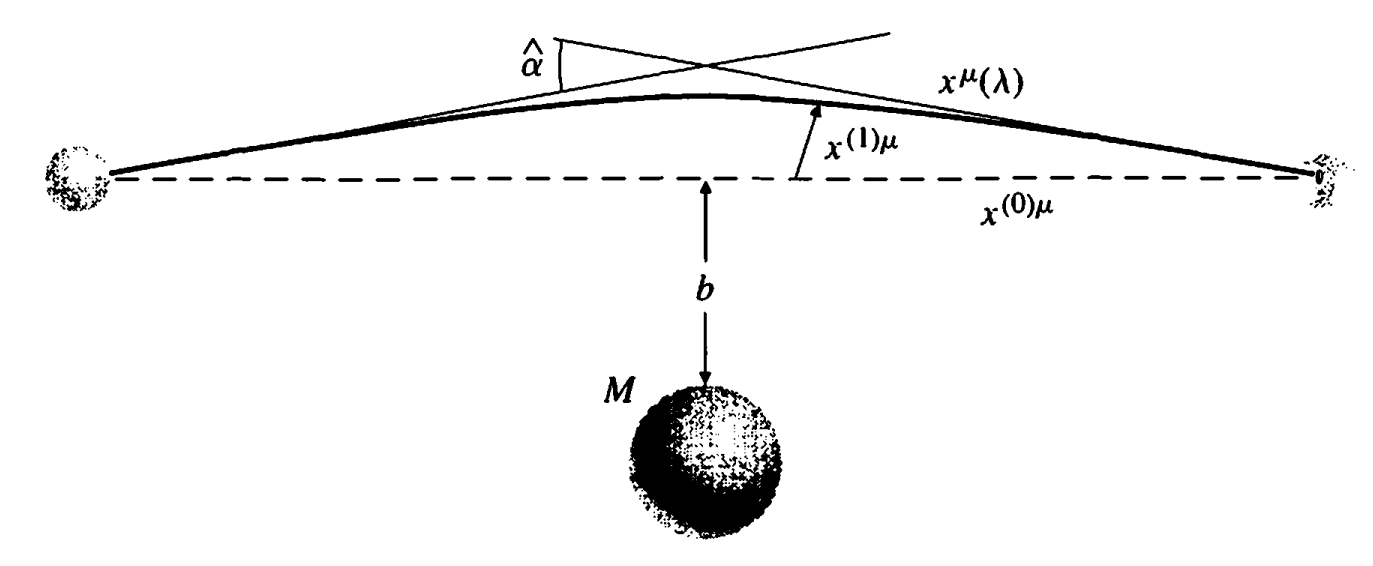
\includegraphics[scale=0.3]{bend}
	\caption{A deflected geodesic $x^\mu(\lambda)$, decomposed into a background geodesic $x^{(0)\mu}$ and a perturbation $x^{(1)u}$. The deflection angle $\hat{\alpha}$ represents (minus) the amount by which the wave vector rotates along the path. A single mass $M$ with impact parameter $b$ is depicted, although the setup is more general.}
\end{figure}

It's important to remember that we consider the metric perturbation as a field defined on a flat background spacetime. With this, we can decompose the geodesic into a background path plus a perturbation:
\begin{align}
x^\mu(\lambda) = x^{(0)\mu}(\lambda) + x^{(1)\mu}(\lambda)
\end{align}
where of course $x^{(0)\mu}(\lambda)$ is just the null (straight) path which solves the flat background geodesic equation. We want to solve for $x^{(1)\mu}(\lambda)$. To do this, we assume that the potential $\phi$ is approximately constant along the background and true geodesics, i.e., $x^{(1)i}\p_i \phi \ll \phi$. This is reasonable assumption, since $x^{(1)\mu}(\lambda)$ is necessarily small. \\

For convenience we denote the derivative of the vector of the background path as $k^\mu$, and the derivative of the deviation vector as $l^\mu$:
\begin{align}
k^\mu \equiv \f{dx^(0)^\mu}{d\lambda}; \quad l^\mu \equiv \f{dx^{(1)\mu}}{d\lambda}.
\end{align}
The null path obeys the condition:
\begin{align}\label{null}
0 &= g_{\mu\nu}\f{dx^\mu}{d\lambda}\f{dx^\nu}{d\lambda}\nn\\
&= \lp \eta_{\mu\nu} + h_{\mu\nu} \rp\f{d\lp x^{(0)\mu} + x^{(1)\mu} \rp}{d\lambda}\f{d\lp x^{(0)\nu} + x^{(1)\nu} \rp}{d\lambda}\nn\\
&= \boxed{\lp \eta_{\mu\nu} + h_{\mu\nu} \rp(k^\mu + l^\mu)(k^\nu + l^\nu)}
\end{align}
At zeroth order we only have 
\begin{align}
\eta_{\mu\nu}k^\mu k^\nu = 0 \implies {\lp k^0\rp}^2 = \vec{k}^2 \equiv k^2.
\end{align}
This defines the constant $k$. At first order, we have
\begin{align}\label{orth}
2\eta_{\mu\nu}k^\mu l^\nu + h_{\mu\nu}k^\mu k^\nu = 0 \implies \boxed{-kl^0 + \vec{l}\cdot \vec{k} = 2k^2 \phi(r)}
\end{align}
since $\lp k^0\rp^2 = \vec{k}^2 = k^2$. Now, we turn to the perturbed geodesic equation:
\begin{align}
\f{d^2 x^\mu}{d\lambda^2} + \Gamma^\mu_{\rho\sigma}\f{dx^\rho}{d\lambda}\f{dx^\sigma}{d\lambda} = 0.
\end{align}
With $\eta_{\mu\nu} = \text{diag}(-\,+\,+\,+)$, the relevant Christoffel symbols are
\begin{align}
&\Gamma^0_{0i} = \Gamma^i_{00} = \p_i \phi\nn\\
&\Gamma^i_{jk} = \delta_{jk}\p_i \phi - \delta_{ik}\p_j\phi - \delta_{ij}\p_k \phi.
\end{align}
The zeroth-order equation simple tells us that $x^{(0)\mu}$ is a straight trajectory, while at first-order we have
\begin{align}
\boxed{\f{d l^\mu}{d\lambda} = -\Gamma^\mu_{\rho\sigma}k^\rho k^\sigma}
\end{align}
When $\mu= 0$, we have
\begin{align}
\boxed{\f{d l^0}{d\lambda} = -2k(\vec{k}\cdot \grad{\phi})}
\end{align}
while the spatial components read
\begin{align}\label{rotate}
\boxed{\f{d\vec{l}}{d\lambda}} &= -2k^2\lp \grad - \vec{\nabla}_\parallel \rp  \phi \nn\\
&\equiv -2k^2\vec{\nabla}_\perp \phi = \boxed{-2k^2\lp \grad{\phi} - k^{-2}(\vec{k}\cdot \grad{\phi})\vec{k} \rp}
\end{align}
where $\vec{\nabla}_\perp$ denotes the gradient of $\phi$ along the deviation and $\vec{\nabla}_\parallel$ denotes the gradient of $\phi$ along the path. \\

 
Next, we notice that
\begin{align}
l^0 &= \int \f{dl^0}{d\lambda}\,d\lambda\nn\\
&= -2k\int (\vec{k}\cdot \grad{\phi})\,d\lambda\nn\\
&= -2k\int \lp \f{d \vec{x}^{(0)}}{d\lambda}\cdot \grad{\phi}\rp\,d\lambda\nn\\
&= -2k\int \grad{\phi}\cdot d\vec{x}^{(0)}\nn\\
&= -2k\int \p_x \phi \,(\hat{x}\cdot \hat{x})\, d{x}^{(0)}\nn\\
&= -2k \phi.
\end{align}
We can fix the constant of integration by demanding that $l^0 \iff \phi= 0$. It follows from \eqref{orth} that
\begin{align}
\vec{l}\cdot \vec{k} &= 2k^2\phi+ kl^0\nn\\
&=2k^2\phi - 2k^2\phi \nn\\
&= 0.
\end{align}
Thus $\vec{k}\perp \vec{l}$, to first order. This makes intuitive sense if we think about it a little bit.\\

Now, the deflection angle $\hat{\alpha}$ is the amount by which the original spatial wave vector is deflected as it travels from a source to the observer. It is a two-dimensional vector in the plane perpendicular to $\vec{k}$ (by figure) and hence is (anti)-parallel to $\vec{l}$. And by the figure, we can write
\begin{align}
\hat{\alpha} = -\f{\Delta \vec{l}}{k},
\end{align}
where the minus sign accounts for the fact that the deflection angle is measured by an observer looking backward along the photon path. The rotation of the wave vector $\Delta \vec{l}$ can be calculated using \eqref{rotate}:
\begin{align}
\Delta \vec{l} &= \int \f{d\vec{l}}{d\lambda}\,d\lambda \nn\\
&= -2k^2 \int -2k^2\vec{\nabla}_\perp \phi\,d\lambda.
\end{align}  
And with $s = k\lambda$ denoting the physical spatial distance traversed we have
\begin{align}
\boxed{\hat{\alpha} = 2\int \vec{\nabla}_\perp \phi\,ds}
\end{align}
We also have
\begin{align}
\phi(r) = \f{-GM}{r} \implies \phi(x) = \f{-GM}{\sqrt{x^2 + b^2}},
\end{align}
and
\begin{align}
\vec{\nabla}_\perp \phi = \f{d}{db}\phi(x)\hat{b} = \f{GM}{(b^2 + x^2)^{3/2}}\vec{b}.
\end{align}
Putting everything together, followed by a change of variables, we get
\begin{align}
\boxed{\hat{\alpha} = 2GMb\int_{-\infty}^\infty \f{dx}{(b^2 + x^2)^{3/2}} = \f{4GM}{b} = \f{2(1+1)GM}{b}}
\end{align}
and so $\gamma=1$ as desired. The integral from $-\infty$ to $\infty$ assumes that both source and observer are very far from the deflecting mass. \\

What if the form of $h_{\mu\nu}$ is 
\begin{align}
{h_{\mu\nu}= \begin{bmatrix}
	-2\phi(r) & &&\\
	&-2\gamma\phi(r)&&\\
	&&-2\gamma\phi(r)&\\
	&&&-2\gamma\phi(r)
	\end{bmatrix}}?
\end{align}
It is not difficult in this case to recalculate the Christoffel symbols, again using $\eta = \text{diag}(-\,+\,+\,+)$ for consistency:
\begin{align}
&\Gamma^\mu_{00} = \p_i \phi\nn\\
&\Gamma^i_{jk} =  \gamma\lp \delta_{jk}\p_i \phi - \delta_{ik}\p_j \phi - \delta_{ij}\p_k \phi\rp.
\end{align}
Repeating the procedure in the previous paragraphs we find from the null path condition \eqref{null} at zeroth order
\begin{align}
\eta_{\mu\nu}k^\mu k^\nu = 0\implies k^2 = \vec{k}^2 = \lp k^0 \rp^2
\end{align}
and at first order, because $\lp k^0 \rp^2 = \vec{k}^2 = k^2$,
\begin{align}
2\eta_{\mu\nu}k^\mu l^\nu + h_{\mu\nu}k^\mu k^\nu = 0 \implies -kl^0 + \vec{l}\cdot \vec{k} = 2(1+\gamma)k^2\phi(r).
\end{align}    
This factor of $(1+\gamma)$ will reappear when we find the spatial component $d\vec{l}/d\lambda$ since it is embedded in the new Christoffel symbol $\Gamma^i_{\mu\nu}$ (I know this must be true, but I won't verify...)
\begin{align}
\boxed{\f{d\vec{l}}{d\lambda} = -2(1+\gamma)k^2 \vec{\nabla}_\perp \phi}
\end{align}
From here and the rest of the procedure, this factor $(1+\gamma)$ is carried throughout (even to the part where we show $\vec{l}\perp \vec{k}$) and eventually end up in the final integral:
\begin{align}
\boxed{\hat{\alpha} = 2(1+\gamma)GMb\int_{-\infty}^\infty \f{dx}{(b^2 + x^2)^{3/2}} = \f{2(1+\gamma)GM}{b}}
\end{align}
So we're done with the massless case. \qedhere \\














\noindent \underline{\textit{Application of \eqref{light}, massive gravity:}}

In the massive case, the metric $h_{\mu\nu}$ has the form
\begin{empheq}[box=\widefbox]{align*}
&h_{00}(r) = \f{2M}{3M_P}\f{1}{4\pi}\f{e^{-mr}}{r}\nn\\
&h_{0i}(r) = 0\nn\\
&h_{ij}(r) = \f{M}{3M_P}\f{1}{4\pi}\f{e^{-mr}}{r}\lb \f{1+mr+m^2r^2}{m^2r^2} \delta_{ij} - \f{1}{m^2 r^4}(3+3mr + m^2r^2)x_ix_j \rb
\end{empheq}
which is not quite the right form to read off the Newtonian potential and light bending. To simplify things, we notice that while the massive gravity action is not gauge invariant, we assumed tat the coupling to the test particle is that of GR, i.e., this coupling is  gauge invariant. We can argue that we are free to make a gauge transformation on the solution $h_{\mu\nu}$, and there will be no effect on the test particle. To simplify the metric above, i.e. hopefully making it more ``uniformly diagonal'' we can go back to the general expression for $h_{ij}$
\begin{align}
h_{ij}(x) = \f{M}{3M_P}\int \f{d^3\mathbf{p}}{(2\pi)^3}e^{i\mathbf{p}\cdot \mathbf{x}}\f{1}{\mathbf{p}^2 + m^2} \lp \delta_{ij} + \f{p_i p_j}{m^2} \rp
\end{align}
and notice that the term $p_ip_j/m^2$ is pure gauge. This means under some gauge transformation, we can ignore this term (why?). With this, our metric is equivalent to the metric:
\begin{align}
&h_{00}(r) = \f{2M}{3M_P}\f{1}{4\pi}\f{e^{-mr}}{r}\nn\\
&h_{0i}(r) = 0\nn\\
&h_{ij}(r) = \f{M}{3M_P}\f{1}{4\pi}\f{e^{-mr}}{r}
\end{align}
In the small mass limit, this metric becomes
\begin{empheq}[box=\widefbox]{align*}
&h_{00}(r) = \f{2M}{3M_P}\f{1}{4\pi r}\nn\\
&h_{0i}(r) = 0\nn\\
&h_{ij}(r) = \f{M}{3M_P}\f{1}{4\pi r}\delta_{ij}
\end{empheq}
which means when we read off the fields $\phi$ and $\psi$ we find 
\begin{align}
h_{00}(r) = \f{2M}{3M_P}\f{1}{4\pi r} \implies \boxed{\phi(r) = -\f{4}{3}\f{GM}{r}}\nn\\
h_{ij}(r) = \f{M}{3M_P}\f{1}{4\pi r}\delta_{ij} \implies \boxed{ \psi(r) = -\f{2}{3}\f{GM}{r}}
\end{align}
for massive gravitons.\\

The Newtonian potential $\phi$ is larger then for the massless case. The PPN parameter is
\begin{align}
\boxed{\gamma = \f{\psi(r)}{\phi(r)} = \f{1}{2}}
\end{align} 
and thus the magnitude of the light bending angle for light incident at impact parameter $b$ is reduced by $25\%$:
\begin{align}
\boxed{\hat{\alpha} = \f{2(1+ 1/2)GM}{b} = \f{3GM}{b} \neq \f{4GM}{b}}
\end{align}
when we scale $\phi$ so that it matches with the Newtonian potential, even in the massless limit (note that this formula is obtained from the massless theory, so we can only use it here in the massless limit). \\

What this all means is that linearized massive gravity, even in the massless limit, gives predictions which are order 1 different from linearized GR. This is the vDVZ discontinuity. It is present in other physical predictions as well, such as emission of gravitational radiation. Sean Carroll's Chapter 7,\textit{Spacetime \& Geometry} goes over how to derive gravitation radiation (gravitational wave), but we won't worry about that.


















\newpage

\subsection{The St\"{u}ckelberg Trick}

There are a number of ways the St\"{u}ckelberg trick has appeared in literature. Some refer to it as an approach or trick. Some don't even refer to it at all. In this section, we look at some approaches to introducing and using the St\"{u}kelberg trick in the context of massive gravity.\\

We have seen that there is a discontinuity in the physical prediction of linear massless gravity and the massless limit of linear massive gravity, known as the vDVZ discontinuity. We will see explicitly that the correct massless limit of massive gravity is not massless gravity, but rather massless gravity plus extra degrees of freedom. The extra degrees of freedom are a massless vector and a massless scalar, which couples to the trace of the energy momentum tensor. This extra scalar coupling is responsible for the vVDZ discontinuity. \\

Recall the Lagrangian:
\begin{empheq}[box=\widefbox]{align*}
S_{FP} = \int d^Dx\, &-\f{1}{2}\p_\lambda h_{\mu\nu} \p^\lambda h^{\mu\nu} + \p_\mu h_{\nu\lambda}\p^\nu h^{\mu\lambda}\nn\\& - \p_\mu h^{\mu\nu}\p_\nu h + \f{1}{2}\p_\lambda h \p^\lambda h -\f{1}{2}m^2\lp h_{\mu\nu}h^{\mu\nu} - h^2 \rp + \kappa h_{\mu\nu}T^{\mu\nu}
\end{empheq}
Taking the $m\to 0$ straight away here does not yield a smooth limit, since degrees of freedom are lost. To find the correct limit, the \textit{trick} is to introduce new fields and gauge symmetries into the massive theory in a way that does not alter the theory. This is called the St\"{u}ckelberg trick. Once this is done, a limit can be found in which no degrees of freedom are gained or lost. 

\subsubsection{Motivation}

The goal of the St\"{u}kelberg trick is to make a massive theory gauge invariant. As we have seen, the massive term in the Fierz-Pauli action breaks diffeomorphism. The St\"{u}kelberg mechanism is the introduction of new field(s) to a reveal a symmetry of a gauge-fixed theory. \\

In general, dynamical tensors $K_{\mu\nu}$ transform under diffeomorphisms as
\begin{align}
K_{\mu\nu} \to &\,\,K_{\mu\nu} + \lag_3 K_{\mu\nu} \nn\\
&= K_{\mu\nu} + (\p_\mu \epsilon^\alpha)K_{\alpha\nu} + (\p_\nu \epsilon^\alpha)K_{\mu\alpha} + \epsilon^\alpha \p_\alpha K_{\mu\nu}.
\end{align}
However, nondynamical background $\bar{K}_{\mu\nu}$ obeys
\begin{align}
\bar{K}_{\mu\nu} \to \bar{K}_{\mu\nu}.
\end{align}

In the context of massive gravity, in the nonlinear regime, we want to couple a mass to $g_{\mu\nu}$. But we also want to avoid $g^{\mu\nu}g_{\mu\nu} = 4$, so we must introduce a nondynamical background $\bar{K}_{\mu\nu}$ such that the mass terms become $\sim (\bar{K}^{\mu\nu}g_{\mu\nu})^2$, which break diffeomorphism.  \\

St\"{u}kelberg's trick puts back diffeomorphism invariance while introducing 4 scalars $\phi^a, a = 0,1,2,3$ such that we gain/lose no degree of freedom. To do this, we can replace
\begin{align}
\bar{K}_{\mu\nu}(x) \to \p_\mu \phi^a \p_\nu \phi^b \bar{K}_{ab}(\phi(x)).
\end{align}
Here $\phi^a$ is a dynamical scalar with which we can restore diffeomorphism invariance in the theory. (We will see later why we would like to make this replacement/definition.)\\

How is diffeomorphism restored? Well first we can fix
\begin{align}
\phi^a = \delta^a_\alpha x^\alpha,
\end{align} 
where $x^\alpha$ is literally just the coordinate, such that
\begin{align}
\p_\mu \phi^a = \delta^a_\alpha \delta^\alpha_\mu = \delta^a_\mu.
\end{align}
So we have
\begin{align}
\p_\mu \phi^a\p_\nu \phi^b \bar{K}_{ab}(\phi) &= \delta^a_\mu \delta^b_\nu \bar{K}_{ab} \nn\\
&= \bar{K}_{\mu\nu}(x).
\end{align}
So we see this choice of gauge fixing gives the desired transformation. Next, suppose we look at excitations of the form
\begin{align}
\phi^a = \delta^a_\alpha(x^\alpha +\pi^\alpha)
\end{align}
where $\pi^\alpha$ are fields that are like th Nambu-Goldstone modes, then
\begin{align}
\p_\mu \phi^a &= \delta^a_\mu + \p_\mu \pi^\alpha \delta^a_\alpha\nn\\
&= \delta^a_\mu + \p_\mu \pi^a.
\end{align}
With this,
\begin{align}
\p_\mu \phi^a \p_\nu \phi^b \bar{K}_{ab} &= (\delta^a_\mu + \p_\mu \pi^a)(\delta^b_\nu + \p_\nu \pi^b)\bar{K}_{ab}(x+\pi)\nn\\
&\approx  (\delta^a_\mu + \p_\mu \pi^a)(\delta^b_\nu + \p_\nu \pi^b)(\bar{K}_{ab} + \pi^\alpha \p_\alpha K_{ab}(x) + \dots)\nn\\
&\approx \bar{K}_{\mu\nu} + (\p_\mu \pi^a)\bar{K}_{a\nu} + (\p_\nu \pi^b)\bar{K}_{\mu b} + \pi^\alpha \p_\alpha \bar{K}_{\mu\nu} + \dots
\end{align}
up to first order in $\pi$. The first approximation is just an affine approximation of $\bar{K}_{ab}$. This puts the Nambu-Goldstone modes back into the theory with explicit breaking, when $\pi^\mu$ are like Nambu-Goldstone modes. This turns out to have local symmetry. We can always gauge fix so that $\p^\mu \to 0$ and get back the original theory. \\

A lot of this seems very arbitrary and sort of ``out-of-nowhere.'' But rest assured, as we will see what we are actually doing by introducing $\phi^a$ and how this trick works in the next section.






\subsubsection{The St\"{u}ckelberg's Trick - a Vector Example (Hinterbichler)}

To see how the trick works, we consider a simple case of the theory of a massive photon $A_\mu$ coupled to a (not necessarily conserved) source $J_\mu$:
\begin{align}
S = \int d^Dx\, -\f{1}{4}F_{\mu\nu}F^{\mu\nu} - \f{1}{2}m^2 A_\mu A^\mu + A_\mu J^\mu.
\end{align}
where of course
\begin{align}
F_{\mu\nu} = \p_\mu A_\nu - \p_\nu A_\mu
\end{align}
is the anti-symmetric EM stress-tensor. The mass term break the would-be gauge invariance:
\begin{align}
A_\mu \to A_\mu + \p_\mu \Lambda \iff \delta A_\mu = \p_\mu \Lambda,
\end{align}
and for $D=4$ this theory describes the 3 degrees of freedom of a massive spin 1 particle. The propagator for this theory is given by
\begin{align}
\f{-i}{p^2 + m^2}\lp \eta_{\mu\nu} +\f{p_\mu p_\nu}{m^2} \rp
\end{align}
which is not quite as nice as the usual massless photon propagator (Maxwell theory) due to $m\neq 0$, and is similar to $\sim 1/m^2$ for large momenta. This property invalidates the usual power-counting arguments.\\

The limit $m\to 0$ of the Lagrangian above is not a smooth limit because we lose a degree of freedom: for $m=0$ we have Maxwell's EM theory which propagates only with 2 degrees of freedom. Also, the limit fails to exist unless $J^\mu$ is conserved. \\

Here's how the St\"{u}ckelberg trick works. The trick consists of introducing a new scalar field $\phi$ such  tat the new action has gauge symmetry but is still dynamically equivalent to the original action. It will give a different $m\to 0$ smooth limit such that no degrees of freedom are gained or lost. \\

Let us begin by introducing  a field $\phi$ by making the replacement:
\begin{align}
A_\mu \to A_\mu + \p_\mu \phi
\end{align}
following the pattern of the gauge symmetry we want to introduce. This is \textit{not} a change of field variables, a decomposition of $A_\mu$, nor a gauge transformation (remember, this new theory breaks gauge invariance). Rather, we are creating a new Lagrangian from th old one, by the addition of a new field $\phi$. $F_{\mu\nu}$ is invariant under this replacement because the replacement is similar to a gauge transformation under which $F_{\mu\nu}$ is invariant. The only thing that changes is the mass term and the coupling to the source. Following some simple algebra, the action becomes
\begin{align}
S = \int d^Dx\, -\f{1}{4}F_{\mu\nu}F^{\mu\nu} -\f{1}{2}m^2\lp A_\mu + \p_\mu \phi \rp^2 + A_\mu J^\mu - \phi \p_\mu J^\mu
\end{align} 
where we have integrated by parts in the coupling to the source. The new action now has the gauge symmetry:
\begin{align}
\delta A_\mu = \p_\mu \Lambda; \quad \delta \phi = -\Lambda.
\end{align}
By fixing the gauge $\phi = 0$, called the unitary gauge, we recover the original Lagrangian:
\begin{align}
S = \int d^Dx\, -\f{1}{4}F_{\mu\nu}F^{\mu\nu} - \f{1}{2}m^2 A_\mu A^\mu + A_\mu J^\mu.
\end{align}
This tells us that the action with $\phi = 0$ and $\phi \neq 0$ are equivalent theories. They both describe the 3 d.o.f of a massive spin 1 in 4-dimensional spacetime. The new Lagrangian just has more fields and symmetries. Pro tip: when introducing new fields, make sure to introduce new symmetries so as to conserve degrees of freedom. \\

The St\"{u}ckelberg trick uses redundancy (introduces new fields as well as new symmetries) to fix theories. The St\"{u}ckelberg trick adds and removes extra gauge symmetry in a way that does not mess with the manifest Lorentz invariance and locality. \\

Now, consider the new theory again:
\begin{align}
S = \int d^Dx\, -\f{1}{4}F_{\mu\nu}F^{\mu\nu} -\f{1}{2}m^2\lp A_\mu + \p_\mu \phi \rp^2 + A_\mu J^\mu - \phi \p_\mu J^\mu.
\end{align} 
By normalizing $\phi \to m^{-1}\phi$, we get
\begin{align}
S = \int d^Dx\, \f{-1}{4}F_{\mu\nu}F^{\mu\nu} -\f{m^2}{2} A_\mu A^\mu - mA_\mu \p^\mu \phi - \f{1}{2}\p_\mu \phi \p^\mu \phi + A_\mu J^\mu-\f{1}{m}\phi \p_\mu J^\mu.
\end{align}
The gauge symmetries after this normalization is:
\begin{align}
\delta A_\mu = \p_\mu \Lambda; \quad \delta \phi = -m\Lambda.
\end{align}
Now, consider the $m\to 0$ limit. If $\p_\mu  J^\mu \neq 0$, i.e., the current is not conserved, then when $m \ll 1$, the scalar field $\phi$ couples strongly with the divergence of source, and the limit does not exist. This requires us to assume the current to be conserved: $\p_\mu J^\mu = 0$. This implies the new theory in the $m\to 0$ limit is 
\begin{align}
\lag = -\f{1}{4}F_{\mu\nu}F^{\mu\nu} - \f{1}{2}\p_\mu \phi \p^\mu \phi + A_\mu J^\mu,
\end{align}
endowed with the gauge symmetries ($m=0$):
\begin{align}
\delta A_\mu = \p_\mu \Lambda; \quad \delta \phi = 0.
\end{align}
The degrees of freedom turn out to be conserved in the limit. For $D=4$ two of the 3 degrees of freedom go into the massless vector,and one goes into the scalar. \\

We can fix a Lorentz-like gauge:
\begin{align}
\p_\mu A^\mu + m\phi = 0
\end{align}
which along with the gauge symmetries: $\delta A_\mu = \p_\mu \Lambda; \quad \delta \phi = -m\Lambda$ satisfies $(\square - m^2)\Lambda = 0$. From Fadeev-Popov, we add a this gauge fixing term (which is zero) to the action to get
\begin{align}
S+ S_{GF} &= S + \int d^Dx\, -\f{1}{2}\lp \p_\mu A^\mu + m\phi \rp^2\nn\\
&= \dots\nn\\
&= \boxed{\int d^Dx\, \f{1}{2}A_\mu (\square - m^2)A^\mu + \f{1}{2}\phi(\square - m^2)\phi + A_\mu J^\mu - \f{1}{m}\phi \p_\mu J^\mu}
\end{align} 
From there, we can pick out the propagators for $A_\mu$ and $\phi$ in momentum space respectively:
\begin{align}
\boxed{\D_{A_\mu}(p) = \f{-i\eta_{\mu\nu}}{p^2 + m^2}; \quad \D_{\phi}(p) = \f{-i}{p^2 + m^2}}
\end{align}
These go as $\sim 1/p^2$ at high momenta. So, we are able to restore good high energy behavior of the theory propagators. 
























\subsubsection{Graviton St\"{u}ckelberg's Trick \& The origin of the vDVZ discontinuity (Hinterbichler)}

Now, let us consider the massive gravity action, which is made up of the massless piece, plus the mass term, plus the source coupling term:
\begin{align}
\boxed{S = \int d^Dx\, \lag_{m=0} - \f{1}{2}m^2\lp h_{\mu\nu}h^{\mu\nu} - h^2 \rp + \kappa h_{\mu\nu}T^{\mu\nu}}
\end{align}
We want to preserve (or restore(?)) the diffeomorphism:
\begin{align}
\delta h_{\mu\nu} = \p_\mu \epsilon_\nu + \p_\nu \epsilon_\mu = \p_{(\mu}\epsilon_{\nu)}
\end{align}
present in the $m=0$ case, so we introduce a St\"{u}ckelberg field $A_\mu$ patterned after the gauge transformation/symmetry:
\begin{align}\label{stuck}
\boxed{h_{\mu\nu} \to h_{\mu\nu} + \p_\mu A_\nu + \p_\nu A_\mu}
\end{align}
What does the action look like following this transformation? Some quick manipulations give
\begin{empheq}[box=\widefbox]{align*}
S = \int d^Dx\, &\lag_{m=0} - \f{1}{2}m^2\lp h_{\mu\nu}h^{\mu\nu} - h^2 \rp - \f{1}{2}m^2 F_{\mu\nu}F^{\mu\nu}\nn\\
&-2m^2\lp h_{\mu\nu} \p^\mu A^\nu - h\p_\mu A^\mu \rp + \kappa h_{\mu\nu}T^{\mu\nu} - 2\kappa A_\mu \p_\nu T^{\mu\nu}
\end{empheq}
where we notice that $\lag_{m=0}$ term is invariant under this transformation (since it is the originally gauge-invariant Lagrangian). Other terms are not invariant under the transformation above in $h_{\mu\nu}$. We also note that we are setting $F_{\mu\nu} = \p_\mu A_\nu - \p_\mu A_\nu$, and that we integrated the last term by parts to bring the $\p$ inside to act on $T^{\mu\nu}$ instead of on $A_\mu$. \\

Just as before, we observe two gauge symmetries:
\begin{align}
\delta h_{\mu\nu} = \p_\mu \epsilon_\nu + \p_\nu \epsilon_\mu; \quad \delta A_\mu = -\epsilon_\mu.
\end{align}
Fixing the gauge $A_\mu = 0$ gives back the massive gravity action (without extra fields, etc.). At this point, if we try to repeat what we did before: rescaling $A_\mu \to m^{-1}A_\mu$, we will fail because when the $m\to 0$ limit is taken, we end up with a massless graviton and a massless photon for a total of 4 degrees of freedom - one less than the desired value of 5. \\

Instead, we go further and introduce a St\"{u}ckelberg field $\phi$ and consider the transformation:
\begin{align}
A_\mu \to A_\mu + \p_\mu \phi,
\end{align}
under which the action above becomes:
\begin{empheq}[box=\widefbox]{align*}
S = \int d^Dx\, &\lag_{m=0} - \f{1}{2}m^2\lp h_{\mu\nu}h^{\mu\nu} - h^2 \rp - \f{1}{2}m^2 F_{\mu\nu}F^{\mu\nu}\nn\\
&-2m^2\lp h_{\mu\nu} \p^\mu A^\nu - h\p_\mu A^\mu \rp -2m^2\lp h_{\mu\nu}\p^\mu \p^\nu \phi - h\square \phi \rp\nn\\
&+\kappa h_{\mu\nu}T^{\mu\nu} - 2\kappa A_\mu \p_\nu T^{\mu\nu} + 2\kappa \phi \p \p T
\end{empheq}
where 
\begin{align}
\p \p T \equiv \p_\mu \p_\nu T^{\mu\nu}.
\end{align}
With the introduction of the scalar field $\phi$, we must also include two more gauge symmetries to the theory, giving 4 total gauge symmetries, which follow from the redefinition \eqref{stuck} 
\begin{align}
\begin{cases}
\delta h_{\mu\nu} = \p_\mu \epsilon_\nu + \p_\nu\epsilon_\mu\nn\\
\delta A_\mu = -\epsilon_\mu \nn\\
\delta A_\mu= \p_\mu \Lambda\nn\\
\delta \phi = -\Lambda.
\end{cases}
\end{align}
Once again, by fixing the gauge $\phi = 0$ we get back the previous Lagrangian. \\

Now, we scale:
\begin{align}
A_\mu &\to \f{1}{m}A_\mu\nn\\
\phi &\to \f{1}{m^2}\phi.
\end{align}
The action changes accordingly as
\begin{empheq}[box=\widefbox]{align*}
S = \int d^Dx\, &\lag_{m=0} - \f{1}{2}m^2\lp h_{\mu\nu}h^{\mu\nu} - h^2 \rp - \f{1}{2} F_{\mu\nu}F^{\mu\nu}\nn\\
&-2m\lp h_{\mu\nu} \p^\mu A^\nu - h\p_\mu A^\mu \rp -2\lp h_{\mu\nu}\p^\mu \p^\nu \phi - h\square \phi \rp\nn\\
&+\kappa h_{\mu\nu}T^{\mu\nu} - \f{2}{m}\kappa A_\mu \p_\nu T^{\mu\nu} + \f{2}{m^2}\kappa \phi \p \p T,
\end{empheq}
and the gauge transformations become:
\begin{align}
\begin{cases}
\delta h_{\mu\nu} = \p_\mu \epsilon_\nu + \p_\nu\epsilon_\mu\nn\\
\delta A_\mu = -m\epsilon_\mu \nn\\
\delta A_\mu = \p_\mu \Lambda\nn\\
\delta \phi = -m\Lambda.
\end{cases}
\end{align}
which is quite obvious since we just rescaled things. Now, in the $m \to  0$ limit, we can see that $A_\mu$ and $\phi$ are strongly coupled to the divergence of the source $\p T$ and $\p \p T$. So suppose that the source $T$ is conserved, in which case $\p_\mu T^{\mu\nu} = 0$, then in this limit the theory takes the form
\begin{align}
\boxed{S = \int d^Dx\, \lag_{m=0}  - \f{1}{2} F_{\mu\nu}F^{\mu\nu}  -2\lp h_{\mu\nu}\p^\mu \p^\nu \phi - h\square \phi \rp +\kappa h_{\mu\nu}T^{\mu\nu} }
\end{align} 
This theory has 5 degrees of freedom: a scalar-tensor vector theory where the vector is completely decoupled ($A_\mu$ is completely contained and isolated in the $F_{\mu\nu}$ term) but the scalar is kinetically mixed with the tensor (the mixed term is the one with $h_{\mu\nu}$ and $\phi$). \\


To unmix the coupling between the tensor field $h_{\mu\nu}$ and the scalar field $\phi$ we introduce a field definition:
\begin{align}\label{new-hh}
\boxed{h_{\mu\nu} = h'_{\mu\nu} + \pi \eta_{\mu\nu}}
\end{align}
where $\pi$ is some scalar field. Under this field substitution, the massless Lagrangian becomes:
\begin{align}
\lag_{m=0}(h) &= -\f{1}{2}\p_\lambda h_{\mu\nu} \p^\lambda h^{\mu\nu} + \p_\mu h_{\nu\lambda}\p^\nu h^{\mu\lambda} - \p_\mu h^{\mu\nu}\p_\nu h + \f{1}{2}\p_\lambda h \p^\lambda h \nn\\
&= \dots\nn\\
&= \lag_{m=0}(h') + (D-2)\lb \p_\mu \pi \p^\mu h' - \p_\mu \pi \p_\nu h'^{\mu\nu} + \f{1}{2}(D-1)\p_\mu \pi \p^\mu \pi \rb.
\end{align}
Now, by setting
\begin{align}
\pi = \f{2}{D-2}\phi,
\end{align}
we can unmix the $h-\phi$ coupling in the original Lagrangian. After some simplifications, we obtain the new action following the field substitution:
\begin{align}
\boxed{S = \int d^Dx\,\lag_{m=0}(h') - \f{1}{2}F_{\mu\nu}F^{\mu\nu} - 2\f{D-2}{D-1}\p_\mu \phi \p^\mu \phi + \kappa h'_{\mu\nu}T^{\mu\nu} + \f{2}{D-2}\kappa \phi T}
\end{align}
The gauge symmetries in this theory are
\begin{align}
\begin{cases}
\delta h'_{\mu\nu} = \p_\mu \epsilon_\nu + \p_\nu \epsilon_\mu \nn\\
\delta A_\mu = 0\nn\\
\delta A_\mu = \p_\mu \Lambda\nn\\
\delta \phi = 0.
\end{cases}
\end{align}
which follow from the field redefinition \eqref{new-hh}. With $D=4$, there are 5 degrees of freedom: two in a canonical massless graviton, two in a canonical massless vector, and one in a canonical massless scalar. \\

However, notice that there is still a coupling between the scalar $\phi$ and the trace of the source $T$ (even) in the $m=0$ limit. This is the origin of the vDVZ discontinuity. When we consider the trajectory of light, we set $T=0$, so this does not affect the bending of light. However, this extra scalar degree of freedom affects the Newtonian potential. We actually have seen this earlier. To reconcile the disagreement in the predicted bending angle of light $\hat{\alpha} \sim 4GM/b \neq 3GM/b$, we will have to rescale the gravitational constant $G$ which affects the Newtonian potential.\\

In the $m\neq 0$ regime with not necessarily conserved source, under the field redefinition:
\begin{align}\label{new-h}
\boxed{h_{\mu\nu} = h'_{\mu\nu} + \f{2}{D-2}\phi \eta_{\mu\nu}}
\end{align}
which follows from setting $\pi = 2\phi/(D-2)$, the full action is given by (ready?)
\begin{empheq}[box=\widefbox]{align*}
S = &\int d^Dx\, \lag_{m=0}(h') - \f{1}{2}m^2 \lp h'_{\mu\nu}h'^{\mu\nu} - h'^2 \rp - \f{1}{2}F_{\mu\nu}F^{\mu\nu}\nn\\
&+ 2\f{D-1}{D-2}\phi \lp \square + \f{D}{D-2}m^2 \rp\phi - 2m\lp h'_{\mu\nu}\p^\mu A^\nu - h' \p_\mu A^\mu \rp + \kappa h'_{\mu\nu}T^{\mu\nu} \nn\\
&+ 2\f{D-1}{D-2}\lp m^2 h'\phi+ 2m \phi \p_\mu A^\mu \rp  +  \f{2}{D-2}\kappa \phi T - \f{2}{m}\kappa A_\mu \p_\nu T^{\mu\nu} + \f{2}{m^2}\kappa \phi \p \p T.
\end{empheq}
(whose verification is left as an ``index-swimming'' exercise to the reader). This theory has the following gauge symmetries:
\begin{align}
\begin{cases}
\delta h'_{\mu\nu} = \p_\mu \epsilon_\nu + \p_\nu \epsilon_\mu + \f{2}{D-2}m \Lambda \eta_{\mu\nu}\nn\\
\delta A_\mu = -m\epsilon_\mu\nn\\
\delta A_\mu = \p_\mu \Lambda\nn\\
\delta \phi = -m\Lambda.
\end{cases}
\end{align}
It looks like the gauge symmetries has drastically changed, but if we look carefully there is not much going on here. From the field redefinition we can see how the first gauge symmetry is obtained:
\begin{align}
h_{\mu\nu} = h'_{\mu\nu} + \f{2}{D-2}\phi \eta_{\mu\nu} \implies \delta h'_{\mu\nu} &= \delta h_{\mu\nu} - \f{2}{D-2}(\delta \phi) \eta_{\mu\nu}\nn\\
&= \p_\mu \epsilon_\nu + \p_\nu \epsilon_\mu - \f{2}{D-2}(\delta \phi) \eta_{\mu\nu}\nn\\
&= \p_\mu \epsilon_\nu + \p_\nu \epsilon_\mu + \f{2}{D-2}m\Lambda \eta_{\mu\nu}
\end{align}
which follows from the fact that
\begin{align}
\delta \phi = -m\Lambda
\end{align}
after defining $A_\mu \to A_\mu + \p_\mu \phi$, and rescaling $A_\mu \to (1/m)A_\mu$ and $\phi \to (1/m^2)\phi$. In any case, these are minor details we don't have to worry about too much. \\

Now, remember that in order to find the propagators for these fields (scalar $\phi$, vector $A_\mu$, and tensor $h_{\mu\nu}$), we must be able to invert the differential operators that correspond to each field in the Lagrangian. Since there are gauge symmetries, these differential operators don't have trivial kernel (i.e. not invertible). This requires some gauge-fixing to allow for operator inversion. There are 2 gauge conditions we would like to fix: one in $\Lambda$ and one in $\epsilon_\mu$. These are the residual ``degrees of freedom'' that we need to eliminate for things to be invertible. \\

We can try to fix the $\epsilon_\mu$ symmetry first. From the gauge symmetries, we observe that if we say
\begin{align}
\p^\nu h'_{\mu\nu} - \f{1}{2}\p_\mu h' + mA_\mu = 0
\end{align}
then we can fix the $\epsilon_\mu$ symmetry up to a residual transformation satisfying
\begin{align}
(\square - m^2)\epsilon_\mu = 0,
\end{align}
which is good, except it is invariant under $\Lambda$ transformations. This requires fixing the $\Lambda$ symmetry. We observe that by fixing 
\begin{align}
\p_\mu A^\mu + m\lp \f{1}{2}h' + 2\f{D-1}{D-2}\phi \rp = 0
\end{align} 
we fix the $\Lambda$ symmetry up to a residual transformation satisfying 
\begin{align}
(\square - m^2)\Lambda = 0.
\end{align}

Thus, we impose the following gauge conditions:
\begin{empheq}[box=\widefbox]{align*}
\p^\nu h'_{\mu\nu} - \f{1}{2}\p_\mu h' + mA_\mu = 0\nn\\
\p_\mu A^\mu + m\lp \f{1}{2}h' + 2\f{D-1}{D-2}\phi \rp = 0
\end{empheq}


Once we have these two gauges, we can add the following gauge-fixing terms (which are just zeros by gauge-fixing)
\begin{align}
\boxed{S_{GF1} = \int d^Dx\, -\lp \p^\nu h'_{\mu\nu} - \f{1}{2}\p_\mu h' + mA_\mu  \rp^2 }
\end{align}
and
\begin{align}
\boxed{S_{GF2} = \int d^Dx\, -\lb \p_\mu A^\mu + m\lp \f{1}{2}h' + 2\f{D-1}{D-2}\phi \rp  \rb^2 }
\end{align}
to the full action (just as we have done before with the original harmonic gauge) to obtain
\begin{empheq}[box=\widefbox]{align*}
S + S_{GF1} + S_{GF2} &= \int d^Dx\, \lb \f{1}{2}h'_{\mu\nu}\lp \square - m^2\rp h'^{\mu\nu} - \f{1}{4}h'\lp \square - m^2 \rp h'\rb\nn\\
&+ \lb A_\mu \lp \square - m^2 \rp A^\mu \rb+ \lb 2\f{D-1}{D-2}\phi   \lp \square - m^2 \rp\phi \rb\nn\\
&\kappa h'_{\mu\nu}T^{\mu\nu} + \f{2}{D-2}\kappa \phi T - \f{2}{m}\kappa A_\mu \p_\nu T^{\mu\nu} + \f{2}{m^2}\kappa \phi \p \p T
\end{empheq}
Recall that the sole purpose of doing this is so that we can write the integrand (the Lagrangian) in terms of the fields and propagators (refer to the part about gauge harmonic for details). In other words, by adding these gauge-fixing terms, we in effect ``diagonalize'' the action. \\

With the action in propagator form, we can read off the propagators of $h'_{\mu\nu}$, $A_\mu$, and $\phi$ respectively:
\begin{align}
\D[h](p) = \f{-i}{p^2 + m^2}\lb \f{1}{2}\lp \eta_{\alpha\sigma}\eta_{\beta\lambda} + \eta_{\alpha\lambda}\eta_{\beta\sigma} \rp - \f{1}{D-2}\eta_{\alpha\beta}\eta_{\sigma\lambda} \rb,
\end{align}
\begin{align}
\D[A](p) = \f{1}{2}\f{-i\eta_{\mu\nu}}{p^2+m^2},
\end{align}
\begin{align}
\D[\phi](p) = \f{D-2}{4(D-1)}\f{-i}{p^2+m^2}
\end{align}
which all behave as $\sim 1/p^2$ at high momenta, so we can apply the usual power-counting methods. These propagators might look a bit unusual, but when we set $D=4$,
\begin{align}
\D[h](p) = \f{-i}{p^2 + m^2}\f{1}{2}\lb \eta_{\alpha\sigma}\eta_{\beta\lambda} + \eta_{\alpha\lambda}\eta_{\beta\sigma}  - \eta_{\alpha\beta}\eta_{\sigma\lambda} \rb,
\end{align}
\begin{align}
\D[A](p) = \f{1}{2}\f{-i\eta_{\mu\nu}}{p^2+m^2},
\end{align}
and
\begin{align}
\D[\phi](p) = \f{1}{6}\f{-i}{p^2+m^2}
\end{align}
we see that these are the propagators we have seen before, and the differential operator-containing terms in the action can be written as
\begin{align}
\int d^Dx\, \f{1}{2} f_{\dots} \mathcal{O}^{\dots} f_{\dots}
\end{align}
for each corresponding field $f$ (scalars, vectors, tensors, etc.) where $\mathcal{O}^{\dots}$ is the inverse of the spatial propagator $\D[f](x)$. I won't worry too much about the details here, because we're not getting any new insights.  






  





\newpage


\subsection{Nonlinear Massive Gravity}

Up to this point, we have studied only the linear theory of massive gravity, which is determined by the requirement that it propagates only one massive spin 2 degree of freedom. We now turn to the study of the possible interactions and non-linearities for massive gravity. 
 

\subsubsection{Massive General Relativity}



Recall the original Einstein-Hilbert action for gravity:
\begin{align}
S = \f{1}{16\pi G}\int d^Dx\, \sqrt{-g}R\equiv \int d^Dx\, \sqrt{-g}M_P^2R
\end{align}
where $R$ is the Ricci scalar, and $M_P \equiv 1/4\pi G$ is the Planck mass. By Hinterbichler's convention, however, $M_P^2 \equiv 1/8\pi G$, so we will be following this convention and write
\begin{align}
S = \f{1}{2\kappa^2}\int d^Dx\, \sqrt{-g}R
\end{align}
where $\kappa  \equiv 1/M_P$ in Hinterbichler's convention. \\

What we want in a full theory of massive gravity is some nonlinear theory whose linear expansion around some background is the massive Fierz-Pauli theory. This theory is no longer GR (or Einstein gravity) in general, because we no longer have an obvious gauge invariance constraint.\\

Our first modification to the original GR is adding the Fierz-Pauli term to the full nonlinear GR action. Doing this implies that all nonlinear interactions are due to GR. The addition of the Fierz-Pauli term is given by
\begin{align}\label{massive}
\boxed{S = \f{1}{2\kappa^2}\int d^Dx\, \lb \sqrt{-g}R - \sqrt{-g^{(0)}}\f{1}{4}m^2 g^{(0)\mu\alpha}g^{(0)\nu\beta}\lp h_{\mu\nu}h_{\alpha\beta} - h_{\mu\alpha}h_{\nu\beta} \rp \rb}
\end{align}
where 
\begin{align}
\boxed{h_{\mu\nu} = g_{\mu\nu} - g^{(0)}_{\mu\nu}}
\end{align}
The Lagrangian now explicitly depends on a fixed metric $g^{(0)}_{\mu\nu}$, called the \textit{absolute metric}, on which the massive graviton $h_{\mu\nu}$ propagates. This means contraction, raising, and lowering of indices of $h_{\mu\nu}$ are done via $g^{(0)}_{}\mu\nu$, and not $g_{\mu\nu}$, which is the full metric. This is similar to what we had before, where $\eta_{\mu\nu}$ was responsible general ``index-manipulation.'' The presence of this absolute metric in the mass term breaks the diffeomorphism invariance of the Einstein-Hilbert term. \\

Varying this action with respect to $g_{\mu\nu}$ (the full metric, NOT the perturbation $h_{\mu\nu}$), we find the following equation of motion
\begin{align}
\boxed{0 = \sqrt{-g}\lp R^{\mu\nu} - \f{1}{2}Rg^{\mu\nu} \rp + \sqrt{-g^{(0)}}\f{m^2}{2}\lp g^{(0)\mu\alpha}g^{(0)\nu\beta}h_{\alpha\beta} - g^{(0)\alpha\beta}h_{\alpha\beta}g^{(0)\mu\nu}\rp}
\end{align} 
(\textbf{Fun Exercise: How was this found?}) We see that because we're varying with respect to the full metric $g_{\mu\nu}$, which contracts (and raises and lowers, etc.) the indices of $R_{\mu\nu}$, we just get back the Einstein tensor $G^{\mu\nu} \equiv R^{\mu\nu} - (1/2)Rg^{\mu\nu}$ for the first term in the action. The second term is bit more tricky. I will get back to how we take the variational derivative of the second term with respect to $g_{\mu\nu}$ later when I have time. We actually don't have to worry too much about this result, since we are interested in a much more general Fierz-Pauli potential. In addition to this, we will later see that we can in fact raise/lower indices of $h$ using $g_{\mu\nu}$, except we must also find the correct relationship between the coefficients in the $g^{(0)}_{\mu\nu}$ and the $g_{\mu\nu}$ variational derivatives.\\

In any case, we observe that if the absolute metric $g^{(0)}_{\mu\nu}$ satisfies the Einstein equations, then $g^{(0)}_{\mu\nu} = g^{\mu\nu} \iff h_{\mu\nu} = 0$ is a solution. In this case, we just get back the original GR. When dealing with massive gravity and more complicated nonlinear solutions thereof, we can have two background structures. On one hand, we can have the \textit{absolute metric}, which breaks diffeomorphism. On the other, there is the background metric, which is a solution to the full nonlinear equations, about which we may expand the action. Often the solution metric we are expanding around will be the same as the absolute metric, but if we were expanding around a different solution, say a black hole, there would be two distinct structures: the black hole solution and the absolute metric.  \\

We are interested in more general interactions beyond the action provided above. We will be adding interaction terms with no derivatives, since these are most important at low energies. The most general such potential which reduces to Fierz-Pauli at quadratic order involves adding terms cubic and higher in $h_{\mu\nu}$ in all possible ways. With this, we write in general:
\begin{align}\label{general-massive}
\boxed{S = \f{1}{2\kappa^2}\int d^Dx\, \lb \sqrt{-g}R - \sqrt{-g^{(0)}}\f{1}{4}m^2 U(g^{(0)},h) \rb}
\end{align}
The interaction potential $U$ is the most general one that reduces to Fierz-Pauli at linear order. The power series representation of this potential $U$ is given by
\begin{align}
U(g^{(0)},h) &= \sum^N_{n=2}U_n(g^{(0)},h) \nn\\
&= U_2(g^{(0)},h) + U_3(g^{(0)},h) + U_4(g^{(0)},h) + U_5(g^{(0)},h) + \dots
\end{align}
where just as before
\begin{align}
U_2(g^{(0)},h) &= g^{(0)\mu\alpha}g^{(0)\nu\beta}\lp h_{\mu\nu}h_{\alpha\beta} - h_{\mu\alpha}h_{\nu\beta} \rp   \nn\\
&= \underbrace{g^{(0)\mu\alpha}g^{(0)\nu\beta}h_{\mu\nu}h_{\alpha\beta}}_{\equiv [h^2]} - \underbrace{g^{(0)\mu\alpha}h_{\mu\alpha}g^{(0)\nu\beta}h_{\nu\beta}}_{\equiv [h]^2}\nn\\
&= [h^2] - [h]^2
\end{align}
and further
\begin{align}
U_3(g^{(0)},h) &= C_1[h^3] + C_2[h^2][h] + C_3[h]^3\nn\\
U_4(g^{(0)},h) &= D_1[h^4] + D_2[h^3][h] + D_3[h^2]^2 + D_4[h^2][h]^2 + D_5[h]^4\nn\\
U_5(g^{(0)},h) &= F_1[h^5] + F_2[h^4][h] + F_3[h^3][h]^2 + F_4[h^3][h^2]\nn\\ &\,\,\,\,\,\,+ F_5[h^2]^2[h] + F_6[h^2][h]^3 + F_7[h]^5\nn\\
&\vdots
\end{align}
The square bracket indicates a trace, with indices raised with $g^{(0)\mu\nu}$:
\begin{align}
&[h] = g^{(0)\mu\nu}h_{\mu\nu},\nn\\
&[h^2] = g^{(0)\mu\nu}h_{\mu\al}g^{(0)\al\be}h_{\nu\beta} \nn\\
&\vdots
\end{align}
The coefficients $C_k$ are generic. Note that the dimension of $\vec{C_k}$ in $U_n(g^{(0)},h)$ whenever $n>D$ is actually redundant by 1, not $n$, because of Cayley-Hamiltonian theorem, which guarantees that existence of combination of the contractions (the combination that is the characteristic polynomial $\lag_h^{TD}(h)$) that annihilates $U_n(g^{(0)}_h)$. This means one of the coefficients in $U_n(g^{(0)},h)$ whenever $n>D$ can be set to zero. \\

For convenience, we will want to reorganize the terms in the potential by raising and lowering with the full metric $g^{\mu\nu}$ rather than the absolute metric $g^{(0)\mu\nu}$, so that we get a common factor of $\sqrt{-g}$ in the action. Under this ``transformation'' we can write the action in terms of the new potential $V(g,h) = U(g^{(0)},h)$:
\begin{align}\label{general-pot}
\boxed{S = \f{1}{2\kappa^2}\int d^Dx\, \lb \sqrt{-g}\lp R - \f{1}{4}m^2 V(g,h) \rp \rb}
\end{align}
where just as before:
\begin{align}
\boxed{V(g,h) = \sum^N_{n=2}V_n(g,h) = V_2(g,h) + V_3(g,h) + V_4(g,h) + V_5(g,h) + \dots}
\end{align}
with 
\begin{align}
V_2(g^{(0)},h) &= g^{\mu\alpha}g^{\nu\beta}\lp h_{\mu\nu}h_{\alpha\beta} - h_{\mu\alpha}h_{\nu\beta} \rp   \nn\\
&= \underbrace{g^{\mu\alpha}g^{\nu\beta}h_{\mu\nu}h_{\alpha\beta}}_{\equiv \langle h^2\rangle } - \underbrace{g^{\mu\alpha}h_{\mu\alpha}g^{\nu\beta}h_{\nu\beta}}_{\equiv \langle h \rangle ^2}= \langle h^2\rangle  - \langle h\rangle ^2\nn\\
V_3(g,h) &= C_1\langle h^3 \rangle  + C_2\langle h^2\rangle \langle h\rangle + C_3\langle h\rangle^3\nn\\
V_4(g,h) &= D_1\langle h^4\rangle  + D_2\langle h^3\rangle \langle h\rangle + D_3\langle h^2\rangle^2 + D_4\langle h^2\rangle\langle h\rangle^2 + D_5\langle h\rangle^4\nn\\
V_5(g,h) &= F_1\langle h^5\rangle  + F_2\langle h^4\rangle\langle h\rangle + F_3\langle h^3\rangle \langle h\rangle^2 + F_4\langle h^3\rangle\langle h^2\rangle\nn\\ &\,\,\,\,\,\,+ F_5\langle h^2\rangle^2\langle h\rangle + F_6\langle h^2\rangle\langle h\rangle^3 + F_7\langle h\rangle^5\nn\\
&\vdots
\end{align}
where the angled brackets are traces with he indices raised with respect to $g^{\mu\nu}$ (not $g^{(0)\mu\nu}$ anymore). It does not matter if we use the full or absolute metric, as long as we correctly relate the coefficients of the two by expanding the inverse full metric and the full determinant in powers of $h_{\mu\nu}$ raise with the absolute metric. The full metric in terms of a power series in $h$ is:
\begin{align}
\boxed{g^{\mu\nu} = g^{(0)\mu\nu} - h^{\mu\nu} + h^{\mu\lambda}\tensor{h}{_\lambda^\nu} - h^{\mu\lambda}\tensor{h}{_\lambda^\sigma}\tensor{h}{_\sigma^\nu} + \dots}
\end{align}
We can actually verify this in xACT with the following commands:
\begin{lstlisting}
Per = Perturbed[g0[a, b], 3] // ExpandPerturbation

FirstOrderOnly1 = h[LI[n_], __] :> 0 /; n > 1;

Per /. FirstOrderOnly1
\end{lstlisting}
The first command gives the 3rd order perturbation of $g^{\mu\nu}$. Now, we want to express the inverse of $g_{\mu\nu} = g^{(0)}_{\mu\nu} + h_{\mu\nu}$ as a power series in $h^{\mu\nu}$. The problem is the first command in xACT gives us the full expansion including higher perturbative $h_{\mu\nu}$ terms, which we don't want. This is where the first command comes in and sets every $h^{\mu\nu}$ of order higher than 1 (in the perturbation sense, not powers of $h$) to zero. The third command applies this condition to the output of the first command and gives:
\begin{figure}[!htb]
	\centering
	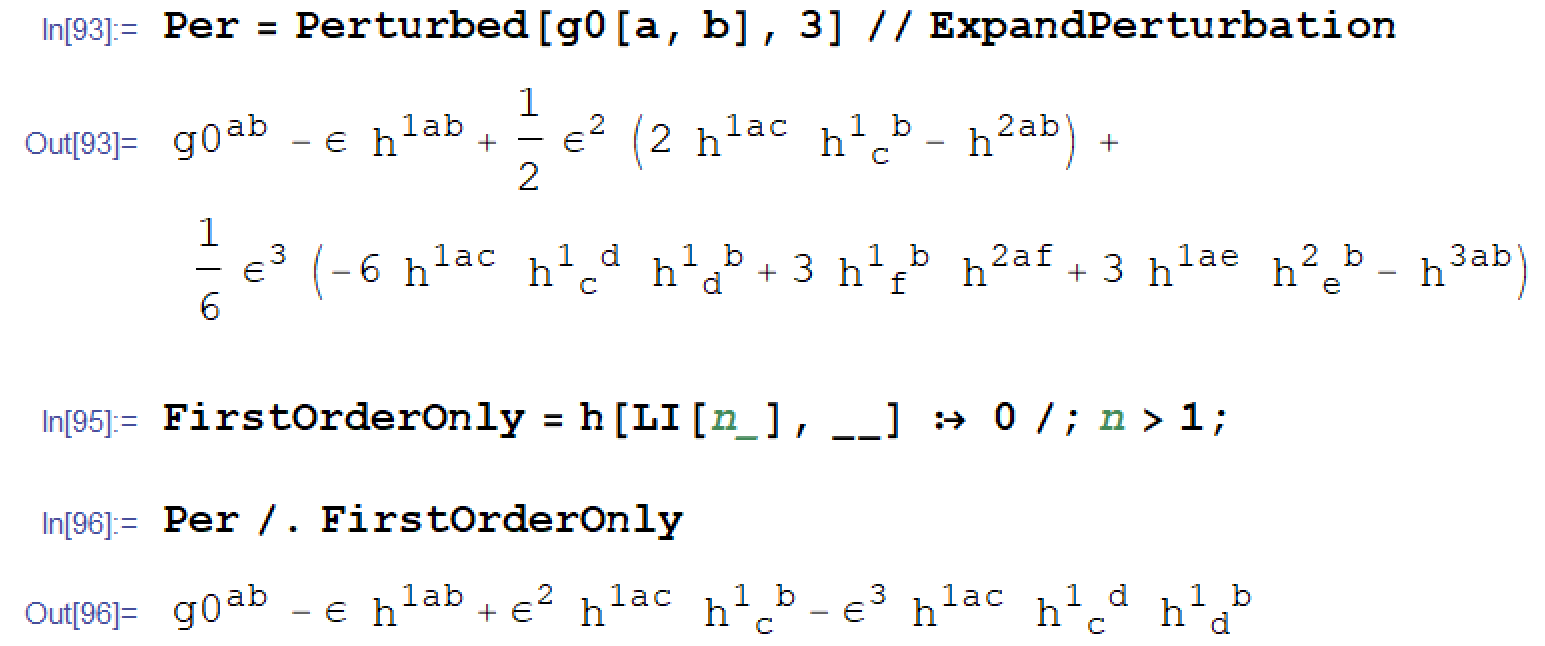
\includegraphics[scale=0.25]{first-order}
\end{figure}



By setting $\epsilon = 1$ we get the desired expansion above. Presumably we should be able to get expansions to very orders of $h$ this way. Let's try order 5:
\begin{figure}[!htb]
	\centering
	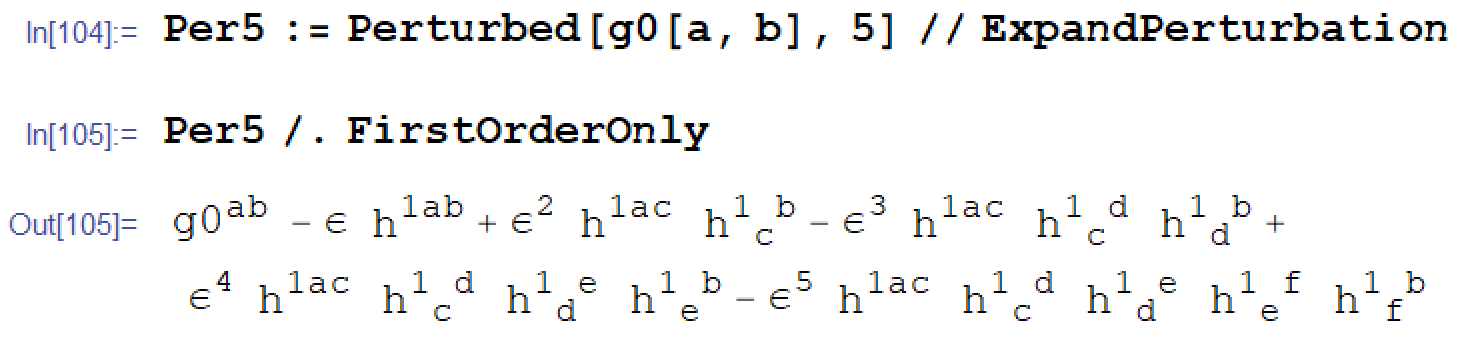
\includegraphics[scale=0.25]{order5}
\end{figure}

in more readable symbols:
\begin{align}
g^{\mu\nu} = g^{(0)\mu\nu} -h^{ab} + h^{ac}\tensor{h}{_c^b} - h^{ac}\tensor{h}{_c^d}\tensor{h}{_d^b} + h^{ac}\tensor{h}{_c^d}\tensor{h}{_d^e}\tensor{h}{_e^b} - h^{ac}\tensor{h}{_c^d}\tensor{h}{_d^e}\tensor{h}{_e^f}\tensor{h}{_f^b} + \dots
\end{align}

We also need to expand the determinant. Hinterbichler says:
\begin{align}
\boxed{\sqrt{-g} = \sqrt{-g^{(0)}}\lb 1 + \f{1}{2}h - \f{1}{4}\lp h^{\mu\nu}h_{\mu\nu} - \f{1}{2}h^2 \rp + \dots \rb}
\end{align}
but I will need to reproduce this somehow, by hand or by xACT. (\textbf{Exercise})\\

We also have the following useful identity:
\begin{align}
\boxed{\langle h^n \rangle = \sum^\infty_{l=0}(-1)^l {{l+n-1}\choose{l}} [h^{l+n}]}
\end{align}
for writing the determinant of $g_{\mu\nu}$ as an expansion in $h_{\mu\nu}$. 






\newpage
\subsubsection{Spherical solutions and the Vainshtein radius}

Next, we look at static spherical solutions. Let $D=4$, and for definiteness we pick the action
\begin{align}
{S = \f{1}{2\kappa^2}\int d^Dx\, \lb \sqrt{-g}R - \sqrt{-g^{(0)}}\f{1}{4}m^2 g^{(0)\mu\alpha}g^{(0)\nu\beta}\lp h_{\mu\nu}h_{\alpha\beta} - h_{\mu\alpha}h_{\nu\beta} \rp \rb}
\end{align}
where the mass term is minimal. We will attempt to find spherically symmetric solutions to the equation of motion
\begin{align}
{0 = \sqrt{-g}\lp R^{\mu\nu} - \f{1}{2}Rg^{\mu\nu} \rp + \sqrt{-g^{(0)}}\f{m^2}{2}\lp g^{(0)\mu\alpha}g^{(0)\nu\beta}h_{\alpha\beta} - g^{(0)\alpha\beta}h_{\alpha\beta}g^{(0)\mu\nu}\rp}
\end{align} 
which we took for granted (good to check/reproduce). We will also assume that the absolute metric is Minkowskian:
\begin{align}
g^{(0)}_{\mu\nu}dx^\mu dx^\nu = -dt^2 + dr^2 + r^2 d\Omega^2
\end{align}
where we're using the $(-,+,+,+)$ convention. We thus consider a spherically symmetric solution (hopefully a good ansatz) whose line element is
\begin{align}
g_{\mu\nu}dx^\mu dx^\nu = -B(r)dt^2 + C(r)dr^2+ A(r)r^2d\Omega^2.
\end{align}
Here we're of course assuming (and hoping) that our ansatz works and is diagonal, or else we will get mixed $r,t,\Omega$ terms in the line element. \\

Next, we recall the identity:
\begin{align}
[F(r)\delta_{ij} + G(r)x_ix_j]dx^idx^j = [F(r) + r^2 G(r)]dr^2 + F(r)r^2d\Omega^2.
\end{align}
Based on the ansatz, we have the following:
\begin{align}
&A(r) \equiv F(r)\nn\\
&C(r) \equiv F(r) + r^2 G(r)
\end{align}
Now, we recall from last time where we found a spherical solution to the easier problem involving $h_{\mu\nu}$. We started with the matrix elements $h_{00}$, $h_{0i}$, and $h_{ij}$ and expressed these in terms of the appropriate $F(r), G(r), -B(r)$. Here we're doing kind of the reverse process where we're starting with the spherical ansatz. Now, we wish to use the equations of motion to write down the relationship among these spherical solutions $F(r), G(r), -B(r)$. How do we do this?\\

Since we've assumed the solution is diagonal, we can rely on the $tt,rr$, and $\theta\theta \equiv \phi\phi$ equations of motion. In order to get the desired results in the end, we can set
\begin{align}
&g_{00}(r) = -B(r)\nn\\
&g_{0i}(r) = 0\nn\\
&g_{ij}(r) = A(r)\delta_{ij} + G(r)x_ix_j 
\end{align}
and define 
\begin{align}
C(r) \equiv A(r) + r^2 G(r).
\end{align}
As matrices:
\begin{align}
\boxed{[g_{\mu\nu}]_{\text{Cartesian}} = \begin{pmatrix}
-B(r) &&&\\
&A(r) + x^2G(r)&xyG(r)&xzG(r)\\
&yxG(r)&A(r)+ y^2G(r)&yzG(r)\\
&zxG(r)&zyG(r)&A(r)+ z^2G(r)
\end{pmatrix}}
\end{align}
and
\begin{align}
[g^{(0)}_{\mu\nu}]_{\text{Spherical}} = \begin{pmatrix}
-1 &&&\\
&1& & \\
&&r^2&\\
&&&r^2 \sin^2\theta \end{pmatrix}
\end{align}
We start by evaluating $\sqrt{-g}$. This can be done in Mathematica:
\begin{lstlisting}
In[2]:= Det[{{-B, 0, 0, 0},
{0, A + x^2*G, x*y*G, x*z*G},
{0, y*x*G, A + y^2*G, y*z*G},
{0, z*x*G, z*y*G, A + z^2*G}}]

Out[2]= -B (A^3 + A^2 G x^2 + A^2 G y^2 + A^2 G z^2)
\end{lstlisting}
The output says the determinant of the $[g_{\mu\nu}]$ matrix is 
\begin{align}
-B(r)A^2(r)\lb A + \underbrace{(x^2 + y^2 + z^2)}_{r^2}G(r) \rb = -A^2B\underbrace{(A+r^2G)}_{C(r)} = -A^2BC.  
\end{align}
So, ${\sqrt{-g} = \sqrt{A^2BC}}$.  Next, we want to evaluate $\sqrt{-g^{(0)}}$. However, note that $[g_{\mu\nu}^{(0)}]$ is in spherical coordinates, while $[g_{\mu\nu}]$ is in Cartesian coordinates. We wish to be consistent, so we will just evaluate $\sqrt{-g^{(0)}}$ ``by analogy'' by reading off the numbers from the line element. Because
\begin{align}
g^{(0)}_{\mu\nu}dx^\mu dx^\nu &= -dt^2 + dr^2 + r^2 d\Omega^2 \nn\\
&= -(1)dt^2 + \lp 1 + 0 r^2 \rp dr^2 + (1)r^2d\Omega^2\nn\\
\text{and }  g_{\mu\nu}dx^\mu dx^\nu &= -B(r)dt^2 + C(r)dr^2+ A(r)r^2d\Omega^2\nn\\
&= -B(r)dt^2 + \lp A(r) + G(r) r^2 \rp dr^2+ A(r)r^2d\Omega^2
\end{align}
and because $\sqrt{-g} = \sqrt{A^2BC}$, we just have $\sqrt{-g^{(0)}} = \sqrt{-1} = 1$, in Cartesian coordinates, as expected. We're also writing the line element wrt $g^{(0)}$ like above so that it resembles the form of $[g_{\mu\nu}]$:
\begin{align}
\boxed{[g^{(0)}_{\mu\nu}]_{\text{Cartesian}} = \begin{pmatrix}
-1 &&&\\
&1 + 0x^2&0xy&0xz\\
&0yx&1+0y^2&0yz\\
&0zx&0zy&1+0z^2
\end{pmatrix} = \begin{pmatrix}
-1 &&&\\
&1&&\\
&&1&\\
&&&1
\end{pmatrix}}
\end{align}
which is also expected. Throughout the derivations, we will be using the boxed matrices as our metrics, both of which are in Cartesian coordinates. \\

With this, we first consider the $tt$ equation:
\begin{align}
{0 = \sqrt{-g}\lp R^{00} - \f{1}{2}Rg^{00} \rp + \sqrt{-g^{(0)}}\f{m^2}{2}\lp g^{(0)0\alpha}g^{(0)0\beta}h_{\alpha\beta} - g^{(0)\alpha\beta}h_{\alpha\beta}g^{(0)00}\rp}
\end{align}
We will unpack the second term first. Recall that
\begin{align}
h_{\mu\nu} = g_{\mu\nu} - g_{\mu\nu}^{(0)}.
\end{align}
So
\begin{align}
g^{(0)0\alpha}g^{(0)0\beta}h_{\alpha\beta} &= g^{(0)0\alpha}g^{(0)0\beta}\lp g_{\al\be} - g_{\al\be}^{(0)} \rp\nn\\
&= \underbrace{g^{(0)00}g^{(0)00}}_{1}\lp g_{00} - g_{00}^{(0)} \rp\nn\\
&= -B(r) + 1,
\end{align}
and
\begin{align}
g^{(0)\alpha\beta}h_{\alpha\beta}g^{(0)00} &= g^{(0)\alpha\beta}g^{(0)00}\lp g_{\al\be} - g_{\al\be}^{(0)}  \rp\nn\\
&= \sum^4_{\alpha=0}\lb g^{(0)\alpha\al}g^{(0)00}\lp g_{\al\al} - g_{\al\al}^{(0)}  \rp  \rb\nn\\
&= \lp-B+1\rp  - \lp A + x^2G -1  \rp -  \lp A + y^2G - 1 \rp - \lp A + z^2G - 1 \rp\nn\\
&= (-B+1) - (3A + r^2G -3).
\end{align}
And so we have successfully dealt with the second term:
\begin{align}
&\sqrt{-g^{(0)}}\f{m^2}{2}\lp g^{(0)0\alpha}g^{(0)0\beta}h_{\alpha\beta} - g^{(0)\alpha\beta}h_{\alpha\beta}g^{(0)00}\rp\nn\\
= &\,\f{m^2}{2}\lb (-B + 1) - (-B+1) - (3A + r^2G-3) \rb\nn\\
= &\,\f{m^2}{2}(-3A - r^2G + 3) \nn\\
= &\,\f{m^2}{2}\lp -3A + 3 - r^2 \f{C-A}{r^2}\rp\nn\\
= &\,\boxed{\f{m^2}{2}\lp  2A + C - 3\rp}
\end{align}
Now comes the difficult part of unpacking the Ricci tensor and scalar. We wish to evaluate the term
\begin{align}
R^{00} - \f{1}{2}Rg^{00}
\end{align}
for $\mu = \nu = 0$. First, $g^{00} = -1/B$ trivially. But what about $R^{00}$ and $R$? We will rely on Mathematica. Part of the calculations is done based on the Mathematica code provided by \href{https://arxiv.org/pdf/0904.4184.pdf}{\underline{Catalogue of Spacetimes}}. \\

\href{https://huanqbui.com/LaTeX projects/HuanBui_QM/Cartesian_Vainshtein.nb}{\underline{Here}} is the link to the notebook, which contains just the calculations for the $tt$ equation. There will be another notebook with the spherical calculations for the other $rr,\theta\theta\equiv \phi\phi$ equations as well. \textit{I'm writing this from the future... the solution below is found using Cartesian coordinates instead of spherical. While it is correct (and I have checked many times to make sure it was correct) it is very, very, cumbersome. The new notebook contains the spherical calculations for this $tt$ equation as well. If the reader is curious and wants to download a notebook to view the calculations, I recommend downloading the other notebook, link in the section where we derive the $rr$-equation.} The notebook requires no additional packages. It should run on any basic Mathematica installation. \\
 
We first clear some symbols, define the dimensions, metric, etc:
\begin{lstlisting}
Clear[coord, metric, inversemetric, affine, t, x, y, z]

r := Sqrt[x^2 + y^2 + z^2]

n := 4

coord := {t, x, y, z}

metric := {{-B[r], 0, 0, 0},
{0, A[r]+x^2*(-A[r]+C[r])/r^2, x*y*(-A[r]+C[r])/r^2, x*z*(-A[r] + C[r])/r^2},
{0, y*x*(-A[r]+C[r])/r^2, A[r]+y^2*(-A[r]+C[r])/r^2, y*z*(-A[r] + C[r])/r^2},
{0, z*x*(-A[r]+C[r])/r^2, z*y*(-A[r]+C[r])/r^2, A[r] + z^2*(-A[r]+C[r])/r^2}}
\end{lstlisting}
Note that the metric $g_{\mu\nu}$ we should be using here must be in terms of $B(r), A(r), C(r)$, since we ultimately want solutions in terms of these functions. In matrix form, $[g_{\mu\nu}]$ is
\begin{align}
\boxed{[g_{\mu\nu}] = \begin{pmatrix}
	-B &&&\\
	&A + x^2\lp \f{C-A}{r^2} \rp&xy\lp \f{C-A}{r^2} \rp&xz\lp \f{C-A}{r^2} \rp\\
	&yx\lp \f{C-A}{r^2} \rp&A+ y^2\lp \f{C-A}{r^2} \rp&yz\lp \f{C-A}{r^2} \rp\\
	&zx\lp \f{C-A}{r^2} \rp&zy\lp \f{C-A}{r^2} \rp&A+ z^2\lp \f{C-A}{r^2} \rp
	\end{pmatrix}}
\end{align}
It is easy to check that $\sqrt{-g} = \sqrt{A^2BC}$ by brute forcing in Mathematica. I won't reproduce the results here. \\

Next, we find the inverse metric, in order to set up for calculations of Christoffel symbols, Riemann, Ricci tensors, and the Ricci scalar. 
\begin{lstlisting}
inversemetric := Simplify[Inverse[metric]]
\end{lstlisting}
Every now and then, we define ``rules''  to force-simplify things. \\

Next, we calculate Christoffel symbols of the 2nd kind:
\begin{lstlisting}

Calculating the Christoffel symbols of the second kind: 

rule1 = {A[Sqrt[
x^2 + y^2 + z^2]] + (x^2 + y^2 + z^2) G[Sqrt[
x^2 + y^2 + z^2]] -> C[r]};

affine := affine = 
Simplify[Table[(1/2) Sum[
inversemetric[[Mu, Rho]] (D[metric[[Rho, Nu]], coord[[Lambda]]] + 
D[metric[[Rho, Lambda]], coord[[Nu]]] - 
D[metric[[Nu, Lambda]], coord[[Rho]]]), {Rho, 1, n}], {Nu, 1, 
n}, {Lambda, 1, n}, {Mu, 1, n}]]

listaffine := 
Table[If[UnsameQ[affine[[Nu, Lambda, Mu]], 
0], {Style[
Subsuperscript[\[CapitalGamma], Row[{coord[[Nu]], coord[[Lambda]]}], 
coord[[Mu]]], 18], "=", Style[affine[[Nu, Lambda, Mu]], 14]}], {Lambda, 
1, n}, {Nu, 1, Lambda}, {Mu, 1, n}]

Simplify[TableForm[Partition[DeleteCases[Flatten[listaffine], Null], 3], 
TableSpacing -> {1, 2}] /. rule1]
\end{lstlisting}

This outputs an entire table of nontrivial Christoffel symbols which we won't worry about. Here's a snippet of the output:
\begin{figure}[!htb]
	\centering
	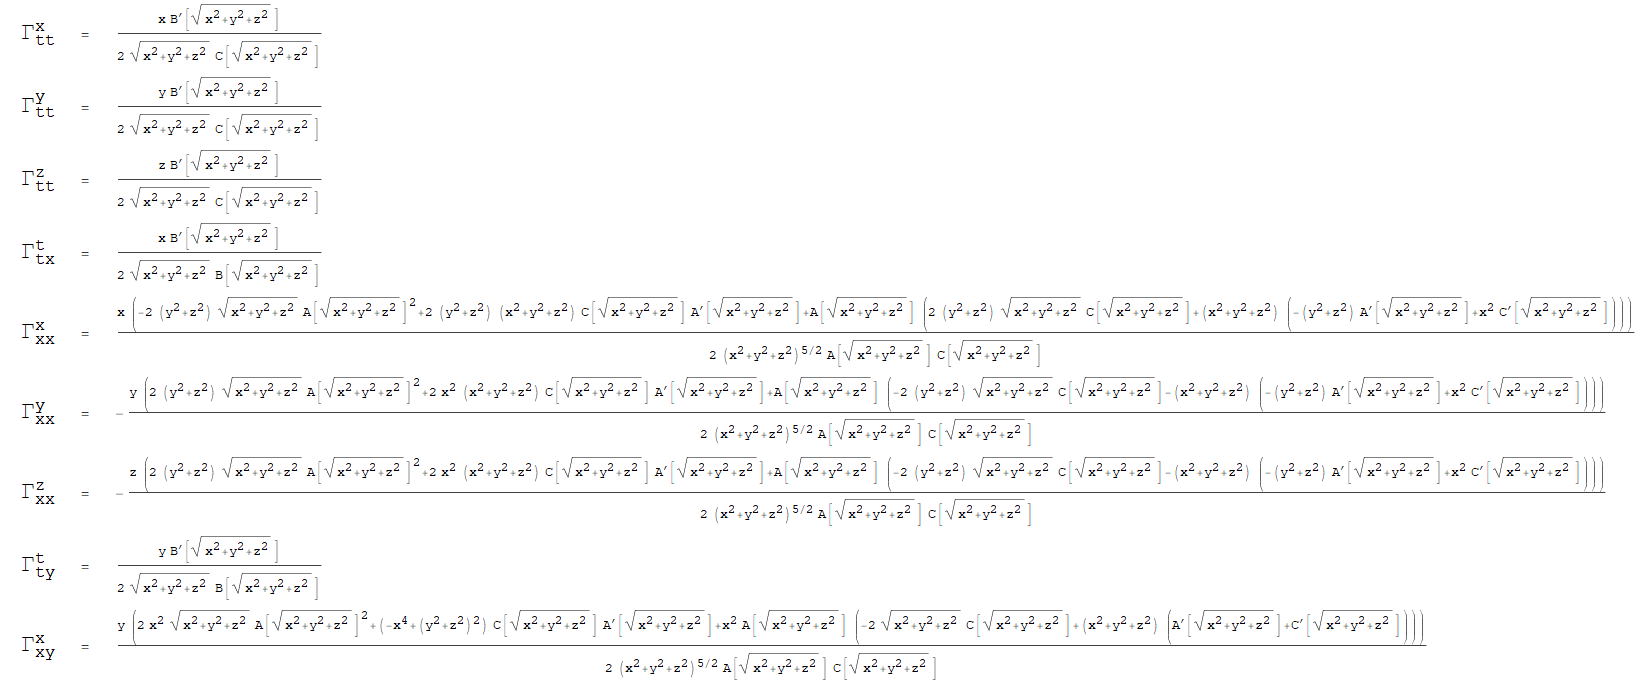
\includegraphics[scale=0.3]{christoffel}
\end{figure}

Next, we define and compute the lower-index Riemann tensors:
\begin{lstlisting}
Defining the Riemann tensor.

riemann := 
riemann = Table[
D[affine[[Nu, Sigma, Mu]], coord[[Rho]]] - 
D[affine[[Nu, Rho, Mu]], coord[[Sigma]]] + 
Sum[affine[[Rho, Lambda, Mu]] affine[[Nu, Sigma, Lambda]] - 
affine[[Sigma, Lambda, Mu]] affine[[Nu, Rho, Lambda]], {Lambda, 1, 
n}], {Mu, 1, n}, {Nu, 1, n}, {Rho, 1, n}, {Sigma, 1, n}]



Defining the Riemann tensor with lower indices.

riemannDn := 
riemannDn = 
Table[Simplify[
Sum[metric[[Mu, Kappa]] riemann[[Kappa, Nu, Rho, Sigma]], {Kappa, 1, 
n}]], {Mu, 1, n}, {Nu, 1, n}, {Rho, 1, n}, {Sigma, 1, n}]

listRiemann := 
Table[If[UnsameQ[riemannDn[[Mu, Nu, Rho, Sigma]], 
0], {Style[
Subscript[R, 
Row[{coord[[Mu]], coord[[Nu]], coord[[Rho]], coord[[Sigma]]}]], 16], 
"=", riemannDn[[Mu, Nu, Rho, Sigma]]}], {Nu, 1, n}, {Mu, 1, Nu}, {Sigma, 
1, n}, {Rho, 1, Sigma}]

Simplify[Simplify[
TableForm[Partition[DeleteCases[Flatten[listRiemann], Null], 3], 
TableSpacing -> {2, 2}] /. rule1] /. rule1]
\end{lstlisting}

There are (obviously) a lot of them. Here are some:
\begin{figure}[!htb]
	\centering
	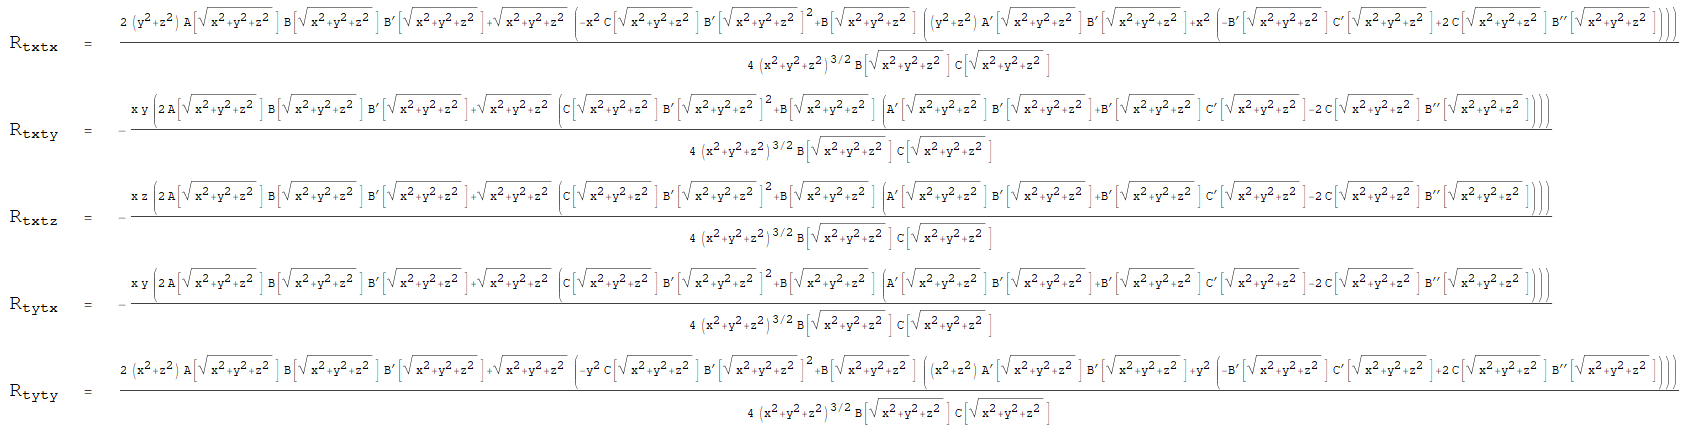
\includegraphics[scale=0.25]{riemann}
\end{figure}

Almost there... Next, we define the Ricci tensors:
\begin{lstlisting}
Defining Ricci tensor:

ricci := ricci = 
Table[Simplify[Sum[riemann[[Rho, Mu, Rho, Nu]], {Rho, 1, n}]], {Mu, 1, 
n}, {Nu, 1, n}]

listRicci := 
Table[If[UnsameQ[ricci[[Mu, Nu]], 
0], {Style[Subscript[R, Row[{coord[[Mu]], coord[[Nu]]}]], 16], "=", 
Style[ricci[[Mu, Nu]], 16]}], {Nu, 1, 4}, {Mu, 1, Nu}]

TableForm[Partition[DeleteCases[Flatten[listRicci], Null], 3], 
TableSpacing -> {1, 2}]
\end{lstlisting}
There aren't too many of these, but no expression is short enough to fit the width of the page, so I will just include $R_{tt}$ and truncated versions of $R_{xx}, R_{yy},\dots$
\begin{figure}[!htb]
	\centering
	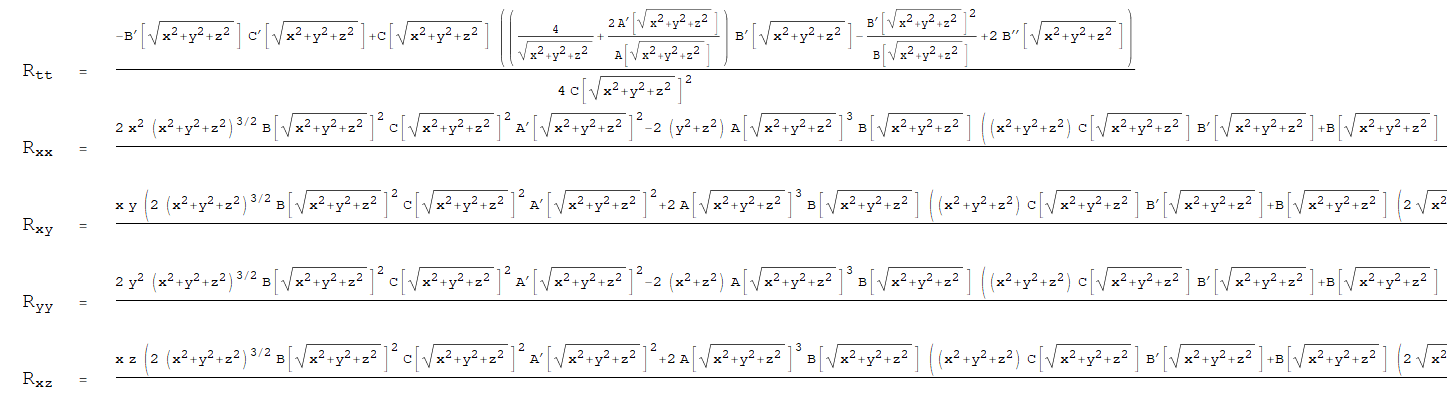
\includegraphics[scale=0.3]{riccitensors}
\end{figure}

Okay. Moving on to the last item: the Ricci scalar.
\begin{lstlisting}
Defining Ricci scalar:

ricciscalar := 
ricciscalar = 
Simplify[Sum[
Sum[inversemetric[[Mu, Nu]] ricci[[Nu, Mu]], {Mu, 1, n}], {Nu, 1, n}]]

Simplify[Simplify[ricciscalar]]
\end{lstlisting}
The output isn't very useful to work with:
\begin{figure}[!htb]
	\centering
	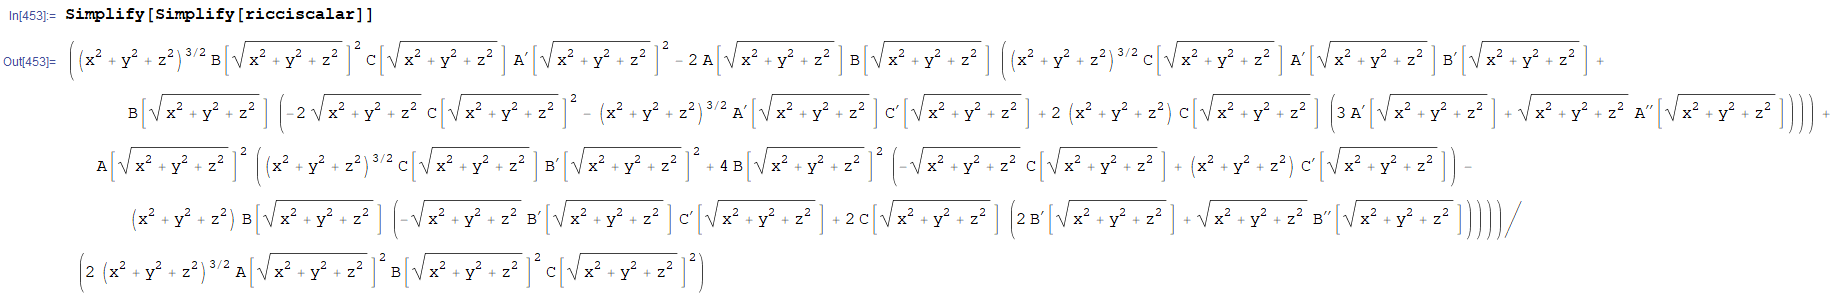
\includegraphics[scale=0.25]{ricciscalar}
\end{figure}
so we will define more rules to simplify it to a useful form:
\begin{lstlisting}
rule2 = {Sqrt[x^2 + y^2 + z^2] -> R};

rule3 = {(x^2 + y^2 + z^2)^(-1/2) -> R^(-1)};

rule4 = {(x^2 + y^2 + z^2)^(3/2) -> R^3};

rule5 = {(x^2 + y^2 + z^2) -> R^2};

rule6 = {Sqrt[R^2]^(-1) -> R^(-1)};

RR = Simplify[
Simplify[Simplify[
Simplify[
Simplify[
Simplify[Simplify[ricciscalar] /. rule1] /. rule2] /. 
rule3] /. rule4] /. rule5] /. rule6]

(1/(2 R^2 A[R]^2 B[R]^2 C[
R]^2))(R^2 B[R]^2 C[R] Derivative[1][A][R]^2 + 
2 A[R] B[R] (-R^2 C[R] Derivative[1][A][R] Derivative[1][B][R] + 
B[R] (2 C[R]^2 + R^2 Derivative[1][A][R] Derivative[1][C][R] - 
2 R C[R] (3 Derivative[1][A][R] + 
R (A^\[Prime]\[Prime])[R]))) + 
A[R]^2 (R^2 C[R] Derivative[1][B][R]^2 - 
4 B[R]^2 (C[R] - R Derivative[1][C][R]) + 
R B[R] (R Derivative[1][B][R] Derivative[1][C][R] - 
2 C[R] (2 Derivative[1][B][R] + R (B^\[Prime]\[Prime])[R]))))
\end{lstlisting}
In symbols:
\begin{figure}[!htb]
	\centering
	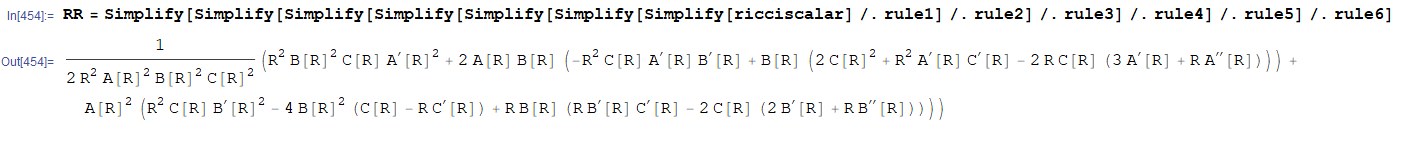
\includegraphics[scale=0.32]{ricciscalar1}
\end{figure}

Now, we want the quantity, which is LeftTerm minus RightTerm
\begin{align}
R^{00} - \f{1}{2}Rg^{00} \equiv \text{LeftTerm} - \text{RightTerm}. 
\end{align}
The \textbf{LeftTerm} is obtained from raising the indices of $R_{\mu\nu}$. This turned out not to be very difficult, because $g^{0\nu}$ entries are all zero except at $\nu = 0$ where $g^{00} = -1/B$. We need two of these to raise the indices of $R_{\mu\nu}$, so as a result we have $R^{00} = (1/B^2)R_{00}$. The \textbf{Rtt} term in the code below is just $R^{00}$.

\begin{lstlisting}
LeftTerm := 
Simplify[Simplify[
Simplify[
Simplify[
Simplify[Simplify[Rtt /. rule1] /. rule2] /. rule3] /. 
rule4] /. rule5] /. rule6];

RightTerm := 
Simplify[Simplify[
Simplify[
Simplify[
Simplify[Simplify[(1/2)*RR*(-1/B[R]) /. rule1] /. rule2] /. 
rule3] /. rule4] /. rule5] /. rule6];

LeftTerm - RightTerm
\end{lstlisting} 

The \textbf{RightTerm} is just $(1/2)Rg^{00}$. The output is
\begin{figure}[!htb]
	\centering
	\includegraphics[scale=0.3]{leftright}
\end{figure}

Next, we define more rules to help with simplifying things:
\begin{lstlisting}
rule7 = {(2 C[R]^2 + R^2 Derivative[1][A][R] Derivative[1][C][R] - 
2 R C[R] (3 Derivative[1][A][R] + R (A^\[Prime]\[Prime])[R])) ->
STUFF1};

Simplify[LeftTerm - RightTerm /. rule7]

rule8 = {R^2 C[R] Derivative[1][A][R]^2 -> STUFF2};

Simplify[Simplify[LeftTerm - RightTerm /. rule7] /. rule8]

rule9 = {-4 A[R]^2 (C[R] - R Derivative[1][C][R]) -> STUFF3};

Simplify[Simplify[
Simplify[LeftTerm - RightTerm /. rule7] /. rule8] /. rule9]

rule10 = {2 STUFF1 A[R] -> STUFF4};

Simplify[Simplify[
Simplify[Simplify[LeftTerm - RightTerm /. rule7] /. rule8] /. 
rule9] /. rule10]

rule11 = {STUFF2 + STUFF3 + STUFF4 -> STUFF5};

Simplify[Simplify[
Simplify[
Simplify[Simplify[LeftTerm - RightTerm /. rule7] /. rule8] /. 
rule9] /. rule10] /. rule11]
\end{lstlisting}


We expand the final output and look for things to cancel:
\begin{lstlisting}

Simplify[Simplify[
Simplify[
Simplify[Simplify[LeftTerm - RightTerm /. rule7] /. rule8] /. 
rule9] /. rule10] /. rule11] // ExpandAll

\end{lstlisting}
\begin{figure}[!htb]
	\centering
	\includegraphics[scale=0.3]{outputt}
\end{figure}

Do you see where things cancel? \\
\begin{figure}[!htb]
	\centering
	\includegraphics[scale=0.3]{outputtt}
\end{figure}




So we're left with just
\begin{align}
R^{00} - \f{1}{2}Rg^{00} = \f{r^2C(A')^2 - 4A^2(C-rC') + 2A\lp 2C^2+r^2A'C'-2r(3A'+rA'')C \rp}{4r^2A^2BC^2}.
\end{align}
Next, we bring in the square root of minus the determinant of $g$:
\begin{align}
&\sqrt{-g}\lp R^{00} - \f{1}{2}Rg^{00} \rp \nn\\
= &\sqrt{A^2BC} \f{r^2C(A')^2 - 4A^2(C-rC') + 2A\lp 2C^2+r^2A'C'-2r(3A'+rA'')C \rp}{4r^2A^2BC^2}.
\end{align}

And... we have the $tt$ equation:
\begin{align}
0 &= \sqrt{-g}\lp R^{00} - \f{1}{2}Rg^{00} \rp + \sqrt{-g^{(0)}}\f{m^2}{2}\lp g^{(0)00\al}g^{(0)0\be}h_{\al\be} - g^{(0)\al\be}h_{\al\be}g^{(0)00} \rp \nn\\
0 &= \sqrt{A^2BC}\lc{r^2C(A')^2 - 4A^2(C-rC') + 2A\lp 2C^2+r^2A'C'-2r(3A'+rA'')C \rp}\rc\nn\\
&\quad  + \f{m^2}{2}\lp  2A + C - 3\rp(4r^2A^2BC^2)
\end{align}
The simplified form, the \textbf{$tt$ equation} is:
\begin{empheq}[box=\widefbox]{align}
0 &=  4BC^2m^2r^2A^3 + [2B(C-3)C^2m^2r^2 - 4\sqrt{A^2BC}(C-rC')]A^2 \nn\\
&\quad\quad 2\sqrt{A^2BC}[2C^2-2r(3A'+rA'')C+r^2A'C']A + C\sqrt{A^2BC}r^2(A')^2
\end{empheq}

Next, we find the $rr$ equation. It is at this point that we realized we've been doing things the HARD WAY by working in Cartesian coordinates. There's a reason, however. In Cartesian coordinates, the determinant of $g_{\mu\nu}$ does not have dependence on $r$ and $\sin\theta$. In spherical coordinates, there is dependence on $\theta$, but I think that because the $\sin\theta$ term appears in both the determinant of the $g$ metric and the Minkowskian metric, we can just ignore it because the LHS must be zero.\\

In any case, we learned something by taking the Cartesian route. We will soon see how well-behaved things become once we go to spherical coordinates. I have uploaded a \href{https://huanqbui.com/LaTeX projects/HuanBui_QM/SphericalSolution_Vainshtein.nb}{\underline{new Mathematica notebook}} with the actual, full, spherical solution. This notebook contains the derivation of the $tt$ equation as well.  \\

From here on, we will be using metrics in spherical coordinates. From the specified line elements, the metrics are:
\begin{align}
\boxed{[g_{\mu\nu}] = \begin{pmatrix}
	-B &&&\\
	&C&&\\
	&&Ar^2&\\
	&&&Ar^2\sin^2\theta
	\end{pmatrix}}
\end{align}
and
\begin{align}
\boxed{[g^{(0)}_{\mu\nu}] = \begin{pmatrix}
	-1 &&&\\
	&1&&\\
	&&r^2&\\
	&&&r^2\sin^2\theta
	\end{pmatrix}}
\end{align}

Let us redefine everything in terms of spherical coordinates in the notebook and go over the calculations again. Trust me this will be quick.
\begin{lstlisting}
Clear[coord, metric, inversemetric, affine, t, r, \[Theta], \[Phi]]

n := 4

coord := {t, r, \[Theta], \[Phi]}

metric := {{-B[r], 0, 0, 0},
{0, C[r], 0, 0},
{0, 0, r^2*A[r], 0},
{0, 0, 0, r^2*Sin[\[Theta]]^2*A[r]}}

inversemetric := Simplify[Inverse[metric]]


Calculating the Christoffel symbols of the second kind: 

affine := affine = 
Simplify[Table[(1/2) Sum[
inversemetric[[Mu, Rho]] (D[metric[[Rho, Nu]], coord[[Lambda]]] + 
D[metric[[Rho, Lambda]], coord[[Nu]]] - 
D[metric[[Nu, Lambda]], coord[[Rho]]]), {Rho, 1, n}], {Nu, 1, 
n}, {Lambda, 1, n}, {Mu, 1, n}]]

listaffine := 
Table[If[UnsameQ[affine[[Nu, Lambda, Mu]], 
0], {Style[
Subsuperscript[\[CapitalGamma], Row[{coord[[Nu]], coord[[Lambda]]}], 
coord[[Mu]]], 18], "=", Style[affine[[Nu, Lambda, Mu]], 14]}], {Lambda, 
1, n}, {Nu, 1, Lambda}, {Mu, 1, n}]

Simplify[TableForm[Partition[DeleteCases[Flatten[listaffine], Null], 3], 
TableSpacing -> {1, 2}] /. rule1]
\end{lstlisting}


Here are the Christoffel symbols in spherical coordinates:
\begin{figure}[!htb]
	\centering
	\includegraphics[scale=0.3]{sphericalchristoffel}
\end{figure}

Let the calculations continue...
\begin{lstlisting}
Defining the Riemann tensor.

riemann := 
riemann = Table[
D[affine[[Nu, Sigma, Mu]], coord[[Rho]]] - 
D[affine[[Nu, Rho, Mu]], coord[[Sigma]]] + 
Sum[affine[[Rho, Lambda, Mu]] affine[[Nu, Sigma, Lambda]] - 
affine[[Sigma, Lambda, Mu]] affine[[Nu, Rho, Lambda]], {Lambda, 1, 
n}], {Mu, 1, n}, {Nu, 1, n}, {Rho, 1, n}, {Sigma, 1, n}]



Defining the Riemann tensor with lower indices.

riemannDn := 
riemannDn = 
Table[Simplify[
Sum[metric[[Mu, Kappa]] riemann[[Kappa, Nu, Rho, Sigma]], {Kappa, 1, 
n}]], {Mu, 1, n}, {Nu, 1, n}, {Rho, 1, n}, {Sigma, 1, n}]

listRiemann := 
Table[If[UnsameQ[riemannDn[[Mu, Nu, Rho, Sigma]], 
0], {Style[
Subscript[R, 
Row[{coord[[Mu]], coord[[Nu]], coord[[Rho]], coord[[Sigma]]}]], 16], 
"=", riemannDn[[Mu, Nu, Rho, Sigma]]}], {Nu, 1, n}, {Mu, 1, Nu}, {Sigma, 
1, n}, {Rho, 1, Sigma}]

Simplify[Simplify[
TableForm[Partition[DeleteCases[Flatten[listRiemann], Null], 3], 
TableSpacing -> {2, 2}] /. rule1] /. rule1]
\end{lstlisting}

\begin{figure}[!htb]
	\centering
	\includegraphics[scale=0.4]{sphericalriemann}
\end{figure}


Then comes the Ricci quantities:
\begin{lstlisting}
Defining Ricci tensor:

ricci := ricci = 
Table[Simplify[Sum[riemann[[Rho, Mu, Rho, Nu]], {Rho, 1, n}]], {Mu, 1, 
n}, {Nu, 1, n}]

listRicci := 
Table[If[UnsameQ[ricci[[Mu, Nu]], 
0], {Style[Subscript[R, Row[{coord[[Mu]], coord[[Nu]]}]], 16], "=", 
Style[ricci[[Mu, Nu]], 16]}], {Nu, 1, 4}, {Mu, 1, Nu}]

TableForm[Partition[DeleteCases[Flatten[listRicci], Null], 3], 
TableSpacing -> {1, 2}]

Defining Ricci scalar:

ricciscalar := 
ricciscalar = 
Simplify[Sum[
Sum[inversemetric[[Mu, Nu]] ricci[[Nu, Mu]], {Mu, 1, n}], {Nu, 1, n}]]

Simplify[Simplify[ricciscalar]]

RR = Simplify[ricciscalar]
\end{lstlisting}

Here's the output:
\begin{figure}[!htb]
	\centering
	\includegraphics[scale=0.4]{sphericalricci}
	\includegraphics[scale=0.4]{sphericalricciscalar}
\end{figure}


Next we consider $R_{rr}$. We want $R^{rr}$, so we simply multiplying $R_{rr}$ by $1/C^2$, because $g_{\mu\nu}$ is diagonal in spherical coordinates. We first consider the term
\begin{align}
R^{rr} - \f{1}{2}Rg^{rr}.
\end{align}
To this end we repeat the process with the LeftTerm and RightTerm earlier to get
\begin{lstlisting}
LeftTerm := 
Simplify[Simplify[
Simplify[Simplify[Simplify[Simplify[Rrr/C[r]^2]]]]]];

RightTerm := 
Simplify[Simplify[
Simplify[Simplify[Simplify[Simplify[(1/2)*RR*(1/C[r])]]]]]];

Simplify[LeftTerm - RightTerm] // ExpandAll // ExpandAll
\end{lstlisting}
\begin{figure}[!htb]
	\centering
	\includegraphics[scale=0.4]{sphericalleftright}
\end{figure}

Of course things cancel again!  Simplifying gives
\begin{figure}[!htb]
	\centering
	\includegraphics[scale=0.4]{sphericalleftrightcancel}
\end{figure}
\begin{figure}[!htb]
	\centering
	\includegraphics[scale=0.4]{simplified}
\end{figure}

\newpage

Next, we consider the term
\begin{align}
\sqrt{-g^{(0)}}\f{m^2}{2}\lp g^{(0)1\al}g^{(0)1\be}h_{\alpha\beta} - g^{(0)\al\be}h_{\al\be}g^{(0)11}  \rp.
\end{align}
Of course the first term is just going to be $h_{11} = C-1$. The second term has some contractions with factors of sines and $r^2$ floating around. But we can do this quickly by ignoring everything that is not the functions $A,B,C$. We can do this because when we multiplying the inverses $g^{(0)\mu\nu}$ with $h_{\mu\nu}$, the $r^2$ and sine factors automatically cancel out. The result is
\begin{align}
\sqrt{-g^{(0)}}\f{m^2}{2}\lp g^{(0)1\al}g^{(0)1\be}h_{\alpha\beta} - g^{(0)\al\be}h_{\al\be}g^{(0)11}  \rp &= \f{-m^2}{2}\lp 2(A-1) - (-B+1) \rp\nn\\
&= \boxed{\f{-m^2(2A+B-3)}{2}}
\end{align}
Putting everything together, we will find the $rr$ equation:
\begin{align}
0 &= \sqrt{-g}\lp R^{rr} - \f{1}{2}Rg^{rr} \rp + \sqrt{-g^{(0)}}\f{m^2}{2}\lp g^{(0)1\al}g^{(0)1\be}h_{\alpha\beta} - g^{(0)\al\be}h_{\al\be}g^{(0)11}  \rp\nn\\
0 &= \f{r^2B(A')^2 + 4A^2(B+rB') + A[-4B(C-rA')+2r^2A'B']}{A^2BC^2r^2}\nn\\
&\quad\quad - \f{2m^2(2A+B-3)}{\sqrt{A^2BC}}
\end{align}
Simplifying this gives the $rr$ equation:
\begin{empheq}[box=\widefbox]{align}
0 &= \f{4(B+rB')A^2 + [2r^2A'B'-4B(C-rA')]A + Br^2(A')^2 }{A^2BC^2r^2}\nn\\
&\quad\quad - \f{2(2A+B-3)m^2}{\sqrt{A^2BC}}
\end{empheq}

Finally, to get the $\theta\theta\equiv\phi\phi$ equation, we go through the process above once more. To make things a little easier, I'll just derive the $\theta\theta$ equation with $R_{\theta\theta}$ instead of $R^{\theta\theta}$. This way, I don't have to worry about factors of contractions, etc. 

\begin{figure}[!htb]
	\centering
	\includegraphics[scale=0.4]{theta}
\end{figure}
This simplifies to 
\begin{figure}[!htb]
	\centering
	\includegraphics[scale=0.4]{thetasimplified}
\end{figure}


On to the $\sqrt{g^{(0)}}$ terms, we compute
\begin{align}
 \sqrt{-g^{(0)}}\f{m^2}{2}\lp g^{(0)2\al}g^{(0)2\be}h_{\alpha\beta} - g^{(0)\al\be}h_{\al\be}g^{(0)22}  \rp.
\end{align}

I won't show the rest of the calculations here. The $\theta\theta\equiv \phi\phi$ equation is
\begin{empheq}[box=\widefbox]{align}
0 &= -2B^2C^2m^2rA^4 - 2B^2C^2(B+C-3)m^2rA^3\nn\\
& - \sqrt{A^2BC}\{2C'B^2 + [rB'C' - 2C(B'+rB'')]B + Cr(B')^2  \}A\nn\\
& +B\sqrt{A^2BC}[CrA'B'+B(4CA'-rC'A'+2CrA'')]A - B^2C\sqrt{A^2BC}r(A')^2.
\end{empheq}
I'll just put the other two equations here, for convenience. The $rr$ equation is
\begin{empheq}[box=\widefbox]{align}
0 &= \f{4(B+rB')A^2 + [2r^2A'B'-4B(C-rA')]A + Br^2(A')^2 }{A^2BC^2r^2}\nn\\
&\quad\quad - \f{2(2A+B-3)m^2}{\sqrt{A^2BC}}
\end{empheq}
The $tt$ equation is
\begin{empheq}[box=\widefbox]{align}
0 &=  4BC^2m^2r^2A^3 + [2B(C-3)C^2m^2r^2 - 4\sqrt{A^2BC}(C-rC')]A^2 \nn\\
&\quad\quad 2\sqrt{A^2BC}[2C^2-2r(3A'+rA'')C+r^2A'C']A + C\sqrt{A^2BC}r^2(A')^2
\end{empheq}


The next step is to solve for $A(r), B(r), C(r)$. To do this we first expand them in the flat space regime, where
\begin{align}
&B_0(r) = 1\\
&A_0(r) = 1\\
&C_0(r) = 1.
\end{align}
To obtain higher order terms, we introduce the expansion
\begin{align}
&B(r) = B_0(r) + \epsilon B_1(r) + \epsilon^2 B_2(r) + \dots\\
&C(r) = C_0(r) + \epsilon C_1(r) + \epsilon^2 C_2(r) + \dots\\
&A(r) = A_0(r) + \epsilon A_1(r) + \epsilon^2 A_2(r) + \dots
\end{align}
Plugging this into the equations we just found and collecting terms of $\mathcal{O}(\epsilon), \mathcal{O}(\epsilon^2),\dots$. This allows us to solve for $B_1,A_1,C_1$, then $B_2,A_2,C_2$, and so on. At $\mathcal{O}(\epsilon)$, we define the expansions in Mathematica only up to $\mathcal{O}(\epsilon)$. (Note: there are probably other ways to do this, but I like it this way. In addition, I will stop including the code because the notebook can be downloaded via the link above. I will just include important outputs from now on. )
\begin{figure}[!htb]
	\centering
	\includegraphics[scale=0.5]{expand}
\end{figure}
Next, we define the $tt,rr,\theta\theta$ equations, using these new function(al)s. (Again, there's probably a more clever and more efficient way to do this, but my method works so far so I'll stick with it.)  
\begin{figure}[!htb]
	\centering
	\includegraphics[scale=0.4]{tt}
	\includegraphics[scale=0.4]{rr}
	\includegraphics[scale=0.4]{thth}
\end{figure}
Once that is done, we must define some rules for simplification. Some of these rules are for helping Mathematica simplify, but some are also important when we extract out $\mathcal{O}(\epsilon)$ terms. 
\begin{lstlisting}
rule12 = {Sqrt[(1 + e A1[r])^2 (1 + e B1[r]) (1 + e C1[r])] -> 1};

rule13 = {Derivative[1][AA][r] -> e*Derivative[1][A1][r]};

rule14 = {(AA^\[Prime]\[Prime])[r] -> e*Derivative[2][A1][r]};

rule15 = {(CC^\[Prime]\[Prime])[r] -> e*Derivative[2][C1][r]};

rule16 = {Derivative[1][CC][r] -> e*Derivative[1][C1][r]};

rule17 = {Sqrt[(1 + e A1[r])^2 (1 + e B1[r]) (1 + e C1[r])]^(-1) -> 1};

rule18 = {(1 + e A1[r])^2 (1 + e B1[r]) (1 + e C1[r]) -> 1};

rule19 = {((1 + e A1[r])^2 (1 + e B1[r]) (1 + e C1[r])^2)^(-1) -> 1};

rule20 = {Derivative[1][BB][r] -> e*Derivative[1][B1][r]};

rule21 = {(BB^\[Prime]\[Prime])[r] -> e*Derivative[2][B1][r]};
\end{lstlisting}
With these rules, we proceed to collect the $\mathcal{O}(\epsilon)$ terms in each equation:
\begin{lstlisting}
ttSim := Coefficient[
tt /. rule12 /. rule13 /. rule14 /. rule15 /. rule16, e] // Simplify

rrSim := rr /. rule12 /. rule13 /. rule14 /. rule15 /. rule16 /. 
rule17 /. rule18 /. rule19 /. rule20 /. rule21

rrSimSim = 
Coefficient[rrSim /. rule12 /. rule13 /. rule14 /. rule15 /. rule16, 
e] // Simplify

ththSim := 
thth /. rule12 /. rule13 /. rule14 /. rule15 /. rule16 /. rule17 /. 
rule18 /. rule19 /. rule20 /. rule21

thSimSim = 
Coefficient[
ththSim /. rule12 /. rule13 /. rule14 /. rule15 /. rule16 /. 
rule17 /. rule18 /. rule19 /. rule20 /. rule21, e] // Simplify
\end{lstlisting}

Some equations are stubborn and require multiple simplifying, but the result is quite satisfying. Here are the coefficients of $\epsilon$ in the $tt,rr,\theta\theta$ equations, respectively:
\begin{figure}[!htb]
	\centering
	\includegraphics[scale=0.4]{e1}
	\includegraphics[scale=0.4]{e2}
	\includegraphics[scale=0.4]{e3}
\end{figure}
Now, these coefficients must all be zero when $A,B,C$ solve the $tt,rr,\theta\theta$ equations, so we have (in more readable symbols):
\begin{align}
&2(m^2r^2-1)A_1+(m^2r^2+2)C_1+2r(-3A_1'+C_1'-rA_1'')= 0\\
&\f{-1}{2}B_1m^2+\lp \f{1}{r^2}-m^2 \rp A_1 + \f{r(A_1'+B_1')-C_1}{r^2} = 0\\
&rA_1m^2+rB_1m^2+rC_1m^2-2A_1'-B_1'+C_1'-rA_1''-rB_1''=0
\end{align}
Okay. To solve for $A_1,B_1,C_1$, we start with simultaneously solving three equations algebraically for $A_1,A_1',A_1''$ in terms of $B,C$ are their derivatives. To do this, we use Mathematica's NSolve:
\begin{lstlisting}
NSolve[{ttSim == 0, rrSimSim == 0, thSimSim == 0}, {A1[r], 
Derivative[1][A1][r], Derivative[2][A1][r]}] // 
Simplify // FullSimplify
\end{lstlisting}
Here I'm storing the solutions in new variables for ease of access:
\begin{figure}[!htb]
	\centering
	\includegraphics[scale=0.4]{AA}
\end{figure}
Once this is done, we write down two equations: (1) $A_1' = \p_r A_1$, and (2) $A_1''=\p_r A_1$, then proceed to algebraically solve this system for $C_1$ and $C_1'$ in terms of $B_1$ and its derivatives. I will only the include the input.
\begin{figure}[!htb]
	\centering
	\includegraphics[scale=0.4]{CC}
\end{figure}
Finally, settings $C_1' - \p_r C_1 = 0$, we get a second-order differential equation for $B_1(r)$:
\begin{figure}[!htb]
	\centering
	\includegraphics[scale=0.4]{BB}
\end{figure}
Of course this simplifies to 
\begin{align}
\boxed{-3rB_1m^2 + 6B_1' + 3rB_1'' = 0}
\end{align}
This can be DSolve'd easily in Mathematica:
\begin{lstlisting}
DSolve[-3 m^2 r B1[r] + 6 Derivative[1][B1][r] + 
3 r (B1^\[Prime]\[Prime])[r] == 0, B1[r], r]
\end{lstlisting}
which says
\begin{align}
B_1(r) = \mathfrak{C_1}\f{e^{-mr}}{r} + \mathfrak{C_2}\f{e^{mr}}{2mr}
\end{align}
where $\mathfrak{C_1}$ and $\mathfrak{C_2}$ are integration constants. Now, when $m\to 0$, $B_1(r)$ must remain finite, so we rule out the other linearly independent solution. This gives 
\begin{align}
{B_1(r) = -\f{8GM}{3}\f{e^{-mr}}{r}}
\end{align}
where the integration constant has been chosen so that we agree with the solution \eqref{mass} obtained from the Green's function. \\

From here, it is \textit{very easy} to get $C_1, A_1$ from $B_1$, because we already solved for these in terms of $B$ and $B,C$ respectively:
\begin{figure}[!htb]
	\centering
	\includegraphics[scale=0.4]{ABC}
\end{figure}
\begin{empheq}[box=\widefbox]{align}
B_1(r) &= -\f{8GM}{3}\f{e^{-mr}}{r}\\
C_1(r) &= -\f{8GM}{3}\f{e^{-mr}}{r}\f{1+mr}{m^2r^2}\\
A_1(r) &= \f{4GM}{3}\f{e^{-mr}}{r}\f{1+mr+m^2r^2}{m^2r^2}
\end{empheq}

So, the $\mathcal{O}(\epsilon)$ problem is done, so we move on to the $\mathcal{O}(\epsilon^2)$ problem. The procedure will be exactly the same, so I will just put the code-outputs here without saying much. Some new rules will be defined along the way to help Mathematica with simplification. Also, so as not to completely ruin the previous code for the $\mathcal{O}(\epsilon)$ problem, I will be using slightly different names for some functions. Thanks to Hinterbichler himself, I will be using a different function, \texttt{SeriesCoefficient[ ]}, for expanding and collecting the $\mathcal{O}(\epsilon^2)$ terms. This is a better way to do things than using just the naive \texttt{Coefficient[..., $\epsilon^2$]} function. First, we redefine the expansions:
\begin{figure}[!htb]
	\centering
	\includegraphics[scale=0.25]{expansions}
\end{figure}

Then we start with our original $tt$, $rr$, and $\theta\theta$ equations:
\begin{figure}[!htb]
	\centering
	\includegraphics[scale=0.25]{tt2}
\end{figure}


\begin{figure}[!htb]
	\centering
	\includegraphics[scale=0.25]{rr2}
	\includegraphics[scale=0.25]{thth2}
\end{figure}

To make Mathematica appropriately expand the series expansion of $B,C,A$ in these equations, we define 
\begin{figure}[!htb]
	\centering
	\includegraphics[scale=0.3]{ruleA}
\end{figure}\\



With this, the $tt$ equation, under the solved $B_1, C_1, A_1$ is given by
\begin{figure}[!htb]
	\centering
	\includegraphics[scale=0.2]{tt2Sim}
\end{figure}\\




Notice that we're now using \texttt{SeriesCoefficient[]} instead of \texttt{Coefficient} like last time. We write
\begin{align}
0 = 
4 (-1 + m^2 r^2) A_2[r] +  \f{1}{9m^4r^6}
 2 e^{-2 m r} \lb 9 e^{2 m r} m^4 r^6 (2 + m^2 r^2) C_2[r] + \right. \nn\\ 
\left.  2 \lp   180 G^2 M^2 + 360 G^2 m M^2 r + 276 G^2 m^2 M^2 r^2 + 
72 G^2 m^3 M^2 r^3\right. \right. \nn\\ 
\left. - 24 G^2 m^4 M^2 r^4 - 16 G^2 m^5 M^2 r^5 - 
12 G^2 m^6 M^2 r^6 \right.\nn\\
\left.  - 27 e^{2 m r} m^4 r^7 A_2'[r] + 
9 e^{2 m r} m^4 r^7 C_2'[r] - 
9 e^{2 m r} m^4 r^8 A_2''[r]    \rp \left.    \rb
\end{align}


We do a similar thing for the $rr$ equation:
\begin{figure}[!htb]
	\centering
	\includegraphics[scale=0.25]{rr2Sim}
\end{figure}
We write
\begin{align}
0 = \f{1}{9 m^4 r^8} 2 e^{-2 m r} \lb -18 e^{2 m r}
m^4 r^6 (-1 + m^2 r^2) A_2[r] - 9 e^{2 m r} m^6 r^8 B_2[r] \right.\nn\\ 
\left. + 
2 \lp 36 G^2 M^2 + 72 G^2 m M^2 r + 116 G^2 m^2 M^2 r^2 + 
136 G^2 m^3 M^2 r^3 \right. \right. \nn\\
\left. + 120 G^2 m^4 M^2 r^4 + 
48 G^2 m^5 M^2 r^5 - 12 G^2 m^6 M^2 r^6 \right.\nn\\
\left. -  9 e^{2 m r} m^4 r^6 C_2[r] + 
9 e^{2 m r} m^4 r^7 A_2'[r] + 
9 e^{2 m r} m^4 r^7 B_2'[r]\rp \left. \rb
\end{align}

Same thing for the $\theta\theta$ equation:
\begin{figure}[!htb]
	\centering
	\includegraphics[scale=0.25]{thth2Sim}
\end{figure}
We write
\begin{align}
0 = \f{2}{9} \lb -\f{216e^{-2mr}G^2M^2}{m^4 r^7} 
-\f{432e^{-2mr}G^2M^2}{m^3 r^6}
-\f{536 e^{-2mr}G^2M^2}{m^2 r^5}
-\f{496 e^{-2mr}G^2M^2}{m r^4}  \right. \nn\\
\left. - \f{400 e^{-2 m r} G^2 M^2}{r^3} 
- \f{256 e^{-2 m r}G^2 m M^2}{r^2} 
- \f{120 e^{-2 m r} G^2 m^2 M^2}{r} - 9 m^2 r B_2[r] 
\right. \nn\\
\left. - 9 m^2 r A_2[r] - 9 m^2 r C_2[r] + 18 A_2'[r] + 9 B_2'[r] - 9 C_2'[r] + 9 r A_2''[r] + 9r B_2''[r] \rb 
\end{align}

Solving $tt=0, rr=0, \theta\theta = 0$ for $A_2, A_2', A_2''$ we get
\begin{figure}[!htb]
	\centering
	\includegraphics[scale=0.25]{A2}
	\includegraphics[scale=0.25]{A2bis}
\end{figure}\\


\newpage
Then we solve for $C_2, C_2'$ from the $A_2$ equations:
\begin{figure}[!htb]
	\centering
	\includegraphics[scale=0.2]{C2}
\end{figure}\\


Setting $C_2' = (\p_r)C_2$ we get the equation for $B_2$:
\begin{figure}[!htb]
	\centering
	\includegraphics[scale=0.17]{B2_new}
\end{figure}\\





We are only interested in the leading order term for $B_2$, we so find it. Plugging $B_2$ back into the $C_2$ and $A_2$ equations and taking their leading terms we get
\begin{figure}[!htb]
	\centering
	\includegraphics[scale=0.17]{A2B2C2}
\end{figure}\\



\newpage

With these, we set $\epsilon \to 1$ plug them back into the original expansion. After some factorizations we get
\begin{empheq}[box=\widefbox]{align}
B(r) &= 1 - \f{8}{3}\f{GM}{r}\lp 1 - \f{1}{6}\f{GM}{m^4r^5} + \dots\rp\nn\\
C(r) &= 1- \f{8}{3}\f{GM}{m^2r^3}\lp 1 - 14\f{GM}{m^4r^5} + \dots \rp\nn\\
A(r) &= 1 + \f{4}{3}\f{GM}{m^2r^3}\lp 1 - 4\f{GM}{m^4r^5} + \dots \rp
\end{empheq}

where the dots represent higher powers in the nonlinearity parameter $\epsilon$. The nonlinearity expansion is an expansion in the parameter $r_V/r$, with
\begin{align}
\boxed{r_V \equiv \lp \f{GM}{m^4} \rp^{1/5}}
\end{align}
is known as the \textbf{Vainshtein} radius. Notice that with this procedure, we can go on to extract solutions at $\mathcal{O}(\epsilon^n)$. However, we won't do that for now.\\







When $m\to 0$, $r_V \to \infty$, and hence the radius beyond which the solution can be trusted gets pushed out to infinity. Vainshtein argued (in 1972) that this perturbation expansion breaks down and says nothing about the true nonlinear behavior of masive gravity in the massless limit. Thus there was reason to hope that the vDVZ discontinuity was merely an artifact of linear perturbation theory, and that the true nonlinear solutions showed a smooth limit. 



\newpage
\subsubsection{Nonlinear Hamiltonian \& The Boulware-Deser mode}

We won't worry too much about this section, except for a few key points. This section deals with the general action with flat absolute metric:
\begin{align}
S = \f{1}{2\kappa^2}\int d^Dx\, \lb \sqrt{-g}R - \f{1}{4}m^2\eta^{\mu\al}\eta^{\nu\beta}\lp h_{\mu\nu}h_{\al\be} - h_{\mu\al}h_{\nu\be}  \rp \rb.
\end{align} 
The free/linearized theory carries 5 degrees of freedom when $D=4$, but this is no longer true when nonlinearities are involved. \\

Under Hamiltonian analysis (which is too complicated to explain here) one can find that when $D=4$ this theory carries 6 df, and so the nonlinear theory carries more df than the linearized theory. Boulware and Deser (1972) argued that the Hamiltonian is not bounded and hence has instabilities. It turns out that this instability is a \textbf{ghost}, \textit{a scalar with a negative kinetic term}, whose mass around a given background can be determined. Boulware and Deser also argued that adding higher terms in $h$ doesn't make the ghost go away. It turns out that it is possible to add appropriate interactions that eliminate the ghost. In $D$ dimensions, there is a $D-2$ parameter family of such interactions. These interactions also turns out to have the effect of raising the maximum energy cutoff at which massive gravity is valid as an effective field theory. This class of theories solves the problem of the Boulware-Deser ghost. \\

We will come back to ghosts in the next subsection. 










\newpage


\subsection{The Nonlinear St\"{u}ckelberg Formalism}


In this section we extend the St\"{u}ckelberg trick to full nonlinear order. This allows us to trace the breakdown in the linear expansion to strong coupling of the longitudinal mode. It also tells us about quantum corrections, the scale of the effective field theory and where it breaks down.  




\subsubsection{St\"{u}kelberg for gravity and the restoration of diffeomorphism invariance}


In this subsubsection we construct the full nonlinear gravitational St\"{u}ckelberg. The paper by Arkani-Hamed et. al. introduces this extensively. \\

The full finite gauge transformation for gravity is
\begin{align}
g_{\mu\nu}(x) \to \f{\p f^\al}{\p x^\mu} \f{\p f^\be}{\p x^\nu} g_{\al\be}(f(x))
\end{align}
where $f(x)$ is any arbitrary gauge function, which must be a diffeomorphism. In massive gravity, gauge invariance is broken only by the mass term. To restore invariance, we introduce a St\"{u}ckelberg field $Y^\mu(x)$ and apply it to the metric $g_{\mu\nu}$:
\begin{align}
\boxed{g_{\mu\nu}(x) \to G_{\mu\nu} = \f{\p Y^\al}{\p x^\mu} \f{\p Y^\be}{\p x^\nu} g_{\al\be}(Y(x))}
\end{align}

The Einstein-Hilbert term $\sqrt{-g}R$ does not change under this substitution, because it is gauge invariant. The substitution looks similar to a gauge transformation with gauge parameter $Y^\mu$, so no $Y$ fields are introduced into the Einstein-Hilbert part of the action.\\

The graviton mass term, however, picks up dependence on $Y's$ in such a way that it will not be invariant under the following gauge transformation:
\begin{align}
&g_{\mu\nu}(x)\to\f{\p f^\al}{\p x^\mu} \f{\p f^\be}{\p x^\nu} g_{\al\be}(f(x))\\
& Y^\mu(x) \to f^{-1}(Y(x))^\mu
\end{align}
with $f(x)$ being the gauge function. This is because the combination $G_{\mu\nu}$ is gauge invariance. To see this we transform $g_{\mu\nu}$:
\begin{align}\label{transf}
G_{\mu\nu} = \p_\mu Y^\al \p_\nu Y^\be g_{\al\be}(Y(x)) \to \p_\mu Y^\al \p_\nu Y^\be [???]
\end{align}
How does $g_{\al\be}(Y(x))$ transform under $f$? To correctly do this transformation, we can start with transforming something easy first, say the scalar field, $\phi$. We know that $\phi(x)$ transforms under $f$ as $\phi \to \phi(f(x))$. We wish to know how $\phi(Y(x))$ transforms under $f$. Well,
\begin{align}
\phi(Y(x)) \equiv \int \,dy \, \phi(y)\delta(y - Y(x)).
\end{align}
Now that $\phi$ has coordinate dependence, $y$, we now how coordinate transforms under $f$: $y\to f(y)$. So, under $f$,
\begin{align}
\phi(Y(x)) \equiv \int \,dy \, \phi(y)\delta(y - Y(x)) \to  \int \,dy \, \phi(f(y))\delta(y - Y(x)) = \phi(f(Y(x))).
\end{align}
You can repeat this procedure for the metric. We know that under $f$,
\begin{align}
g_{\mu\nu} \to \p_\mu f^\al \p_\nu f^\be g_{\al\be}(f(x))
\end{align}
so $g_{\al\be}(Y(x))$ transforms as
\begin{align}
g_{\al\beta}(Y(x)) \to \lp\p_\al f^\lambda\vert_Y\rp \lp \p_\be f^\sigma\vert_Y\rp g_{\lambda\sigma}(f(Y(x))). 
\end{align}
where $\vert_Y$ denotes ``evaluated at $Y$.'' With this, we can complete Eq. \eqref{transf}:
\begin{align}
G_{\mu\nu} = \p_\mu Y^\al \p_\nu Y^\be g_{\al\be}(Y(x)) \to \p_\mu Y^\al \p_\nu Y^\be \lb \p_\al f^\lambda\vert_Y \p_\beta f^\sigma\vert_Y g_{\lambda\sigma}(f(Y(x))) \rb
\end{align}
But that's not all, we want to pull back, using $f^{-1}$, to get $g_{\lambda\sigma}(Y(x))$. To this end, we simple replace instances of $Y$ by $f^{-1}(Y)$, so that the transformation continues as
\begin{align}
G_{\mu\nu} &\to \p_\mu Y^\al \p_\nu Y^\be \lb \p_\al f^\lambda\vert_Y \p_\beta f^\sigma\vert_Y g_{\lambda\sigma}(f(Y(x))) \rb\nn\\
&\to \p_\mu [f^{-1}(Y)]^\al \p_\nu [f^{-1}(Y)]^\be \lb \p_\al f^\lambda\vert_{f^{-1}(Y)} \p_\beta f^\sigma\vert_{f^{-1}(Y)} g_{\lambda\sigma}(f([f^{-1}(Y)])) \rb\nn\\
&= \p_\mu [f^{-1}(Y)]^\al \p_\nu [f^{-1}(Y)]^\be \lb \p_\al f^\lambda\vert_{f^{-1}(Y)} \p_\beta f^\sigma\vert_{f^{-1}(Y)} g_{\lambda\sigma}(Y(x))) \rb\nn\\
&= (\p_\rho [f^{-1}]^\al\vert_Y)( \p_\mu Y^\rho)( \p_\tau [f^{-1}]^\be\vert_Y)( \p_\nu Y^\tau) ( \p_\al f^\lambda\vert_{f^{-1}(Y)})( \p_\beta f^\sigma\vert_{f^{-1}(Y)}) g_{\lambda\sigma}(Y(x))) \nn\\
& \quad\text{(just the chain rule)}\nn\\
&= \delta^\lambda_\rho \delta^\sigma_\tau\p_\mu Y^\rho \p_\nu Y^\tau g_{\lambda\sigma}(Y(x))
\end{align}
where we have used the fact that 
\begin{align}
(\p_\rho [f^{-1}]^\al\vert_Y)( \p_\al f^\lambda\vert_{f^{-1}(Y)}) = \delta^\lambda_\rho
\end{align}
which relies on the calculus fact:
\begin{align}
\p_x f^{-1}(X) = \f{1}{f'(f(x))}.
\end{align}
Putting everything together, we see that
\begin{align}
G_{\mu\nu} \to \dots \to \dots &= \delta^\lambda_\rho \delta^\sigma_\tau\p_\mu Y^\rho \p_\nu Y^\tau g_{\lambda\sigma}(Y(x)) \nn\\
&=\p_\mu Y^\lambda \p_\nu Y^\sigma g_{\lambda\sigma}(Y(x)) \nn\\
&= G_{\mu\nu},
\end{align}
i.e.,
\begin{align}
\boxed{g_{\mu\nu} \to G_{\mu\nu} \to \p_\mu Y^\lambda \p_\nu Y^\sigma g_{\lambda\sigma}(Y(x)) \equiv G_{\mu\nu}}
\end{align}
which says that the combination $G_{\mu\nu}$ is gauge invariant. \\

Now, we expand $Y$ about the identity function
\begin{align}
Y^\al(x) = x^\al + A^\al(x).
\end{align}
Then the gauge-invariant combination $G_{\mu\nu}$ expands as
\begin{align}\label{xpand}
G_{\mu\nu} &= \f{\p Y^\al(x)}{\p x^\mu(x)} \f{\p Y^\be}{\p x^\nu} g_{\al\be}(Y(x))\nn\\
&= \f{\p (x^\al + A^\al)}{\p x^\mu} \f{\p(x^\be + A^\be)}{\p x^\nu} g_{\al\be}(x+A)\nn\\
&= (\delta^\al_\mu + \p_\mu A^\al)(\delta^\be_\nu + \p_\nu A^\be)\lp g_{\al\be} + A^\mu \p_\mu g_{\al\be} + \f{1}{2}A^\mu A^\nu \p_\mu \p_\nu g_{\al\be} +  \text{ h.o.t.s.} \rp\nn\\
&= g_{\mu\nu} + A^\lambda \p_\lambda g_{\mu\nu} + \p_\mu A^\al g_{\al\nu} + \p_\nu A^\al g_{\al\mu} + \f{1}{2} A^\al A^\be \p_\al\p_\be g_{\mu\nu}\nn\\
&\quad  + \p_\mu A^\al \p_\nu A^\beta g_{\al\be} + \p_\mu A^\al A^\be \p_\be g_{\al\nu} + \p_\nu A^\al A^\be \p_\be g_{\mu\al} + \text{h.o.t.s.}
\end{align}

Next, we look at the infinitesimal transformation properties of $g,A,G,Y$ under the infinitesimal general coordinate transforms generated by
\begin{align}
f(x) = x + \xi(x) \implies f^{-1}(x) \approx x - \xi(x)
\end{align}
which is a diffeomorphism. The transformations of $g,A,G,Y$ are given by taking the the Lie derivatives (for more information, refer to the \href{https://huanqbui.com/LaTeX projects/Classical_Fields_Theory/HuanBui_ClassicalFieldTheory.pdf}{\underline{CFT notes}}) - ``C'' for \textit{classical}. The metric tensor transforms via the Lie derivative rule for tensors:
\begin{align}
\boxed{\delta g_{\mu\nu} = \xi^\lambda \p_\lambda g_{\mu\nu} + \p_\mu \xi^\lambda g_{\lambda\nu} + \p_\nu \xi^\lambda g_{\mu\lambda}}
\end{align}
To find how $Y$ transforms under $f$, we just plug $Y$ into the transformation $f$:
\begin{align}
Y^\mu(x) \to f^{-1}(Y(x))^\mu \approx  Y^\mu(x) - \xi^\mu (Y(x))
\end{align}
which gives
\begin{align}
\boxed{\delta Y^\mu = -\xi^\mu (Y)}
\end{align}
and
\begin{align}
\boxed{\delta A^\mu = -\xi(x+A) = -\xi^\mu - A^\al \p_\al \xi^\mu - \f{1}{2}A^\al A^\be \p_\al\p_\be \xi^\mu - \text{ h.o.t.s.}}
\end{align}
The $A^\mu$ are the Goldstone bosons that nonlinearly carry the broken diffeomorphism invariance in massive gravity. The gauge-invariant combination $G_{\mu\nu}$ is of course gauge-invariant:
\begin{align}
\boxed{\delta G_{\mu\nu} = 0} 
\end{align}

With these, we can now St\"{u}ckelberg the general massive gravity action of the form of Eq. \eqref{general-massive}:
\begin{align}
\boxed{S = \f{1}{2\kappa^2}\int d^Dx\, \lb \sqrt{-g}R - \sqrt{-g^{(0)}}\f{1}{4}m^2 U(g^{(0)},h) \rb}
\end{align}
where interaction potential $U$ is the most general one that reduces to Fierz-Pauli at linear order. The Einstein-Hilbert term is intact, while in the mass term we write all $h_{\mu\nu}$'s with lower indices to get rid of the dependence on the absolute metric $g^{(0)}_{\mu\nu}$ (which is also the background metric). We then replace all occurrences of $h_{\mu\nu}$ with$H_{\mu\nu}$ given by
\begin{align}
\boxed{H_{\mu\nu}(x) = G_{\mu\nu}(x) - g^{(0)}_{\mu\nu}(x)}
\end{align}
We then expand $G_{\mu\nu}$ in terms of $A^\lambda$ and $g_{\mu\nu}$ as in Eq. \eqref{xpand} and $Y^\mu$ as $x^\mu + A^\mu(x)$. To linear order in $h_{\mu\nu} \equiv g_{\mu\nu} - g^{(0)}_{\mu\nu}$ and $A_\mu$ we have
\begin{align}
\boxed{H_{\mu\nu} = h_{\mu\nu} + \nabla_\mu^{(0)}A_\nu + \nabla^{(0)}_\nu A_\mu}
\end{align}
where indices on $A$ are lowered with $g^{(0)}_{\mu\nu}$ and $\nabla^{(0)}_\lambda$ denotes covariant derivatives under the absolute metric $g_{\mu\nu}^{(0)}$. (\textit{The derivation is left as an index-manipulation exercise}.)\\

When the background metric is flat, i.e. $g^{(0)}_{\mu\nu} \equiv \eta_{\mu\nu}$, the expansion is
\begin{align}\label{H}
\boxed{H_{\mu\nu} = h_{\mu\nu} + \p_\mu A_\nu + \p_\nu A_\mu + \p_\mu A^\al \p_\nu A_\al + \text{ h.o.t.s.}}
\end{align}
(\textit{Once again, the derivation is left as an exercise in index manipulation}.) The higher order terms are terms with at least one power of $h$. \\

As in the linear case, we also want to introduce a $U(1)$ gauge symmetry, so let
\begin{align}
A_\mu \to A_\mu + \p_\mu \phi.
\end{align}
With this, the expansion for the flat background metric takes the form
\begin{align}\label{H_flat}
H_{\mu\nu} &= h_{\mu\nu} + \p_\mu A_\nu + \p_\nu A_\mu + 2\p_\mu \p_\nu \phi + \p_\mu A^\al \p_\nu A_\al \nn\\
&\quad \p_\mu A^\al \p_\nu \p_\al \phi + \p_\mu\p^\al \phi \p_\nu A_\al + \p_\mu \p^\al \phi \p_\nu \p_\al \phi + \text{ h.o.t.s.}
\end{align}
Similarly, higher order terms are terms with at least one power of $h$. The gauge transformation rules in this case are
\begin{align}\label{gauge_sym}
&\delta h_{\mu\nu} = \p_\mu \xi_\nu + \p_\nu \xi_\mu + \lag_\xi h_{\mu\nu}\\
&\delta \phi = -\Lambda\\
&\delta A_\mu = \p_\mu \Lambda -\xi_\mu - A^\al \p_\al \xi_\mu -\f{1}{2}A^\al A^\be \p_\al \p_\be \xi_\mu - \text{ h.o.t.s.}
\end{align}
where $\lag_\xi$ denotes the Lie derivative. 




\subsubsection{Another way to St\"{u}ckelberg}

In the last section we introduced gauge invariance and the St\"{u}ckelberg fields by replacing the metric $g_{\mu\nu}$ by the invariant combination $G_{\mu\nu}$. This method is good when we have a potential arranged in the form Eq. \eqref{general-massive}. One draw back of this method is that the St\"{u}ckelberg expansion involves an infinite number of terms of higher order in $h_{\mu\nu}$. This is not good when we want to keep track of the $h_{\mu\nu}$'s.\\


In this section, we introduce the St\"{u}ckelberg fields through the background metric $g^{(0)}_{\mu\nu}$, then allow $g_{\mu\nu}$ to transform covariantly. This method is suite to a potential arranged in the form Eq. \eqref{general-pot}:
\begin{align}
\boxed{S = \f{1}{2\kappa^2}\int d^Dx\, \lb \sqrt{-g}\lp R - \f{1}{4}m^2 V(g,h) \rp \rb}
\end{align}
where the difference between this and the previous arrangement is the lack of dependence on $\sqrt{-g^{(0)}}$. This method contains to higher powers of $h_{\mu\nu}$. \\

The replacement to make is 
\begin{align}
\boxed{g_{\mu\nu}^{(0)} \to g_{\al\be}^{(0)} \p_\mu Y^\al \p_\nu Y^\beta}
\end{align}


The $Y^\al(x)$ being introduced are the four St\"{u}ckelberg fields, which despite the index $\al$ are to transform as \textit{scalars} under diffeomorphisms, i.e. 
\begin{align}
Y^\al(x) \to Y^\al(f(x)) \iff \delta Y^\al = \xi^\nu \p_\nu Y^\al
\end{align}
where the second equality follows from Lie derivative rules for infinitesimal transformations (again, see the \href{https://huanqbui.com/LaTeX projects/Classical_Fields_Theory/HuanBui_ClassicalFieldTheory.pdf}{\underline{CFT notes}} for details).\\

In other words, $Y^\al$ does not transform like a vector, despite the index. With this transformation rule, it is easy to see that the replaced $g^{(0)}_{\mu\nu}$, namely, $g_{\al\be}^{(0)} \p_\mu Y^\al \p_\nu Y^\beta$ transforms similar to a metric tensor. \\

This is nice when we are working with the potential of the form Eq. \eqref{general-pot}. First, we lower all indices on the $h_{\mu\nu}$'s in the potential, so that the background metric $g_{\mu\nu}^{(0)}$ appears only through $h_{\mu\nu} \equiv g_{\mu\nu} - g_{\mu\nu}^{(0)}$. Once that this done, we replace all occurrences of $h_{\mu\nu}$ with
\begin{align}
\boxed{h_{\mu\nu} \to H_{\mu\nu} = g_{\mu\nu} - g_{\al\be}^{(0)}\p_\mu Y^\al \p_\nu Y^\be}
\end{align}
Next, we once again expand $Y^\al$ about the identity function:
\begin{align}
Y^\al = x^\al - A^\al
\end{align}
and using $g_{\mu\nu} = g_{\mu\nu}^{(0)} + h_{\mu\nu}$ we have
\begin{align}
\boxed{H_{\mu\nu} = h_{\mu\nu} + g_{\nu\al}^{(0)} \p_\mu A^\al + g_{\mu\al}^{(0)}\p_\nu A^\al - g_{\al\be}^{(0)}\p_\mu A^\al \p_\nu A^\be    }
\end{align}
We note the sign difference in the quadratic term in $A$ compared with Eq. \eqref{H}. \\

Under infinitesimal gauge transformation we have
\begin{align}
&\delta A^\al = -\xi^\al + \xi^\nu \p_\nu A^\al\\
&\delta h_{\mu\nu} = \nabla_\mu^{(0)}\xi_\nu + \nabla_\nu^{(0)}\xi_\mu + \lag_\xi h_{\mu\nu}
\end{align}
where $\lag_\xi$ denotes the Lie derivative. The covariant derivatives are again with respect to $g_{\mu\nu}^{(0)}$. Indices are also lowered/raised with the absolute metric $g_{\mu\nu}^{(0)}$. To linear order, the transformations are
\begin{align}
&\delta A^\al = \xi^\al\\
&\delta h_{\mu\nu} =  \nabla_\mu^{(0)}\xi_\nu + \nabla_\nu^{(0)}\xi_\mu.
\end{align}

When the background is flat, i.e. $g^{(0)}_{\mu\nu} \equiv \eta_{\mu\nu}$, then the replacement becomes
\begin{align}
\boxed{h_{\mu\nu} \to H_{\mu\nu} = h_{\mu\nu} + \p_\mu A_\nu + \p_\nu A_\mu - \p_\mu A^\al \p_nu A^\al}
\end{align}
which is exact. This is unlike Eq. \eqref{H} where there exist higher order terms in $h_{\mu\nu}$. \\

We follow this by (once again) introducing a $U(1)$ symmetry: $A_\mu \to A_\mu + \p_\mu \phi$ to extract the helicity 0 mode. The full expansion this in case (still $g^{(0)}_{\mu\nu} = \eta_{\mu\nu}$) becomes
\begin{align}
H_{\mu\nu} = &h_{\mu\nu} + \p_\mu A_\nu + \p_\nu A_\mu + 2\p_\mu\p_\nu \phi + \p_\mu A^\al \p_\nu A^\al \nn\\
&\quad  \p_\mu A^\al \p_\nu \p_\al \phi + \p_\mu \p^\al \phi \p_\nu A_\al + \p_\mu \p^\al \phi \p_\nu \p_\al \phi.
\end{align}

The gauge transformation rules in this case are
\begin{align}
&\delta h_{\mu\nu} = \p_\mu \xi_\nu + \p_\nu \xi_\mu  + \lag_\xi h_{\mu\nu}\\
&\delta A_\mu = \p_\mu \Lambda - \xi_\mu + \xi^\nu \p_\nu A_\mu\\
&\delta \phi = -\Lambda.
\end{align}









 




























\newpage

\subsubsection{St\"{u}ckelberg formalism by Arkani-Hamed et al. (extra)}


In this section, we look at how \href{https://arxiv.org/pdf/hep-th/0210184.pdf}{\underline{Arkani-Hamed et al.}} formulates the St\"{u}kelberg's trick as ``building blocks for gravity in theory space.''\\

Their construction of the scalar fields $\phi^a$ we just saw is based on ``sites'' and ``links.'' Sites are endowed with different four-dimensional general covariances (GC). Links are actually link fields with suitable non-linear transformation properties. \\

For every site $j$ there is a general coordinate invariance $GC_j$. Each of these invariances is denoted $x^\mu_j \to f^\mu_j(x_j)$ where $x_j$ are the coordinates. We assume (reasonably) that the transformations $f_j$ are smooth and invertible.\\

Link fields allow us to compare objects on different sites, which obey their local $GC_j$. Recall that a field $\psi(x)$ is a scalar field if it transforms under $GC$ given by a transformation $f$ as
\begin{align}
\phi'(x) = \phi(f(x)) = \phi \circ f.
\end{align}
Similarly, a vector $a_\mu(x)$ transforms under $GC$ given by $f$ as
\begin{align}
a'_\mu = \f{\p f^\alpha}{\p x^\mu}(x)a_\alpha(f(x)).
\end{align}
We see how this rule generalizes for tensors. \\

Now, suppose we want to compare two distinct sites $i,j$ with two different coordinate invariances $GC_i$ and $GC_j$. To do this, we need a mapping from site $i$ to site $j$. Define this mapping as the link field $Y_{j\leftarrow i}$, or $Y_{ji}$ for short. Schematically, this is 
\begin{figure}[!htb]
	\centering
	\includegraphics[scale=0.3]{link}
\end{figure}



These are not just any $Y_{ji}$, of course. They have to obey the transformation
\begin{align}
Y_{ji} \to f_j^{-1} \circ Y_{ji} \circ f_i
\end{align}
where the $f_k$'s are the local $GC$ transformations at $i,j$.\\

Suppose we want to compare two fields $\psi_i$ on site $i$ and $\psi_j$ on site $j$. A logical thing to do is transform $\psi_j$ into some field $\Psi$ in $i$ using $Y_{ji}$:
\begin{align}
\Psi = \psi_j \circ Y_{ji}.
\end{align}
Note that $\Psi$ is in $i$ because its input is in $i$. And so this new field $\Psi$ transforms under $GC_i$ as
\begin{align}
\Psi \to \Psi \circ f_i = \Psi(f_i(x^\mu)).
\end{align}
By the same arguments as before, we can generalize this rule to higher-rank tensors using $Y_{ji}$. For a vector field $a_{j\mu}$ in $j$, we can form a new vector field $A_\mu$ in $i$ of the form
\begin{align}
A_\mu(x_i) = \f{\p Y^\alpha}{\p x_i^\mu}(x_i) a_{j\alpha}(Y_{ji}(x_i)).
\end{align}
For a tensor, say $g_{j\mu\nu}(x_i)$ in $j$, we can form a new tensor $G_{\mu\nu}$ in $i$ of the form
\begin{align}
G_{\mu\nu}(x_i) = \f{\p Y^\alpha}{\p x_i^\mu}\f{\p Y^\beta}{x_i^\nu}g_{j\alpha\beta}(Y_{ji}(x_i)).
\end{align}
These transform under $GC_i$ of course, since they live in $i$.\\

So far the construction has been quite abstract, but this screams diffeomorphism invariance, for we require the fields/tensors on one site formed from fields/tensors on another site to transform correctly under the respective general coordinate invariances. \\

Let us consider a special example where we expand $Y$ and $G$ in terms of pions and see how the two general coordinate invariances are realized explicitly. Suppose that $Y_{ji}$ is just the identity map, i.e.,
\begin{align}
Y_{ji}^\mu(x_i) = x^\mu_i.
\end{align}
Then of course $f_i = f_j$ since now $Y_{ji}$ is just a map from a space to itself. Now, let us expand $Y$ around $x$ as
\begin{align}
Y^\alpha(x) = x^\alpha + \pi^\alpha 
\end{align}
where we have dropped indices to avoid drowning in indices later. This is called \textbf{Glodstone boson expansion}, and it is exactly what we ust introduced in the previous section. Here $Y$ plays the role of the scalar fields $\phi$. \\

With this expansion, any tensor $\bar{K}_{\mu\nu}$ in $i$ can be expanded in terms of a tensor $g^j_{\alpha \beta}$ in $j$ as
\begin{align}
\bar{K}_{\mu\nu} &= \f{\p Y^\alpha (x)}{\p x^\mu}\f{\p Y^\beta (x)}{\p x^\nu} K^j_{\alpha\beta}(Y(x)) \nn\\
&= \f{\p (x^\alpha + \pi^\alpha)}{\p x^\mu}\f{\p (x^\beta + \pi^\beta)}{\p x^\nu} K^j_{\alpha\beta}(x + \pi) \nn\\
&= (\delta^\alpha_\mu + \p_\mu\pi^\alpha)(\delta^\beta_\nu + \p_\nu \pi^\beta)\lp K^j_{\alpha\beta} + \pi^\mu \p_\mu K^j_{\alpha\beta} + \f{1}{2}\pi^\mu \pi^\nu \p_\mu \p_\nu K^j_{\alpha\beta} + \dots \rp\nn\\
&= K^j_{\mu\nu} + \pi^\lambda (\p_\lambda g^j_{\alpha\nu}) + (\p_\mu\pi^\alpha)K^j_{\alpha\nu} + (\p_\nu \pi^\alpha)K^j_{\alpha\mu} + \f{1}{2}\pi^\alpha\pi^\beta \p_\alpha\p_\beta K^j_{\mu\nu} \nn\\
&\hspace{0.5cm} + (\p_\mu \pi^\alpha)(\p_\nu \p^\beta)K^j_{\alpha\beta} + (\p_\mu \pi^\alpha)\pi^\beta \p_\beta K^j_{\alpha\nu} + (\p_\nu \pi^\alpha)\pi^\beta \p_\beta K^j_{\mu\alpha} + \dots
\end{align}

        

(\textit{to be continued? This is just an extra section on the formalisms of the St\"{u}ckelberg's trick. I don't think I'll worry too much about it.})




\newpage





\subsection{St\"{u}ckelberg Analysis of Interacting Massive Gravity}


In this section, we set $D = 4$ and apply the St\"{u}ckelberg analysis to the massive GR action \eqref{massive}:
\begin{align}\label{S}
\boxed{S = \f{1}{2\kappa^2}\int d^Dx\, \lb \sqrt{-g}R - \f{1}{4}m^2 \eta^{\mu\alpha}\eta^{\nu\beta}\lp h_{\mu\nu}h_{\alpha\beta} - h_{\mu\alpha}h_{\nu\beta} \rp \rb}
\end{align}
in the case where $g^{(0)}_{\mu\nu} \equiv \eta_{\mu\nu}$, i.e. is flat. To this end, we make the replacement given by Eq. \eqref{H_flat}:
\begin{empheq}[box=\widefbox]{align}
H_{\mu\nu} &= h_{\mu\nu} + \p_\mu A_\nu + \p_\nu A_\mu + 2\p_\mu \p_\nu \phi + \p_\mu A^\al \p_\nu A_\al \nn\\
&\quad \p_\mu A^\al \p_\nu \p_\al \phi + \p_\mu\p^\al \phi \p_\nu A_\al + \p_\mu \p^\al \phi \p_\nu \p_\al \phi + \text{ h.o.t.s.}
\end{empheq}
The higher order terms with $h$ will not be important in this theory.\\



At linear level, this replacement is exactly the same as the linear St\"{u}ckelberg appeared in Section 2.7.5 on the introduction to the St\"{u}ckelberg trick, given by Eq. \eqref{stuck}:
\begin{align}
\boxed{h_{\mu\nu} \to h_{\mu\nu} + \p_\mu A_\nu + \p_\nu A_\mu}
\end{align}



\begin{framed}
	Creating these proofs allows us to have a better understanding of the Vainshtein mechanism. So while some of these are purely index-manipulations, it is useful to see how some of the pieces fit together.\\
	
	Okay so here's the proof. Recall that the massive gravity action in the linear regime is given by
	\begin{align}
	{S = \int d^Dx\, \lag_{m=0} - \f{1}{2}m^2\lp h_{\mu\nu}h^{\mu\nu} - h^2 \rp + \kappa h_{\mu\nu}T^{\mu\nu}}
	\end{align}
	where
	\begin{align}
	- \f{1}{2}m^2\lp h_{\mu\nu}h^{\mu\nu} - h^2 \rp
	\end{align}
	is the mass term. We want to show that under the replacement (only up to linear orders)
	\begin{align}
	H_{\mu\nu} &= h_{\mu\nu} + \p_\mu A_\nu + \p_\nu A_\mu
	\end{align}
	the following mass term
	\begin{align}
	\boxed{S = \f{1}{2\kappa^2}\int d^Dx\, \lb \sqrt{-g}R - \sqrt{-g^{(0)}}\f{1}{4}m^2 g^{(0)\mu\alpha}g^{(0)\nu\beta}\lp h_{\mu\nu}h_{\alpha\beta} - h_{\mu\alpha}h_{\nu\beta} \rp \rb}
	\end{align}
	is exactly the Fierz-Pauli mass term above, where the absolute metric $g^{(0)}_{\mu\nu}$ is identically Minkowskian, $\eta_{\mu\nu}$.\\
	
	\textit{Proof:} 
	Under the replacement given above, we have that
	\begin{align}
	&h_{\mu\al} \to h_{\mu\al} + \p_\mu A_\al + \p_\al A_\mu \nn\\
	&h_{\nu\be} \to h_{\nu\be} + \p_\nu A_\be + \p_\be A_\nu.
	\end{align}
	With these, 
	\begin{align}
	\eta^{\mu\nu}\eta^{\al\be}\lp h_{\mu\al}h_{\nu\be} - h_{\mu\nu}h_{\al\be} \rp 
	&= h^{\mu\nu}h_{\mu\nu} + \p^\mu A^\al h_{\mu\al} + \p^\al A^\mu h_{\mu\al} + \p^\nu A^\be h_{\nu\be} \nn\\
	&\quad +\p^\nu A^\be \p_\nu A_\be + \p^\nu A^\be \p_\be A_\nu + \p^\be A^\nu h_{\nu\be} + \p_\al A_\mu \p^\mu A^\al  \nn\\
	&\quad + \p^\be A^\nu \p_\be A_\nu - \p^\nu A_\nu \tensor{h}{^\al_\al} - \p^\nu A_\nu \p^\be A_\be - \p^\nu A_\nu \p^\al A_\al \nn\\
	&\quad -\tensor{h}{^\mu_\mu}\tensor{h}{^\al_\al} - \tensor{h}{^\mu_\mu}\p^\be A_\be - \tensor{h}{^\mu_\mu}\p_\be A^\be \nn\\
	&\quad - \p_\nu A^\nu \tensor{h}{^\al_\al} - \p^\nu A_\nu \p_\al A^\al - \p_\nu A^\nu \p_\be A^\be\nn\\
	&= h^{\mu\nu}h_{\mu\nu} - h^2  -4(\p A)h - 4(\p A)^2 + 4(\p A)h + 4(\p A)^2\nn\\
	&= h^{\mu\nu}h_{\mu\nu} - h^2.
	\end{align}
	Seriously easy.  The scaling is a bit off but that's okay because we'll canonically normalize these fields later.
\end{framed}


Once we include the higher order terms of $H_{\mu\nu}$, things get a bit messier, but as we have seen in the proof above, a lot of this is just index manipulation and power counting to eliminate higher-order terms. \\

To make the nonlinear trick work, we first have to normalize the fields so that they match the fields of the linear analysis. Using a hat to signify the canonically normalized fields with the same coefficients as used in Section 2.7.5, we have
\begin{align}\label{canon}
&\hat{h} = \f{1}{2}M_P h\\
&\hat{A} = \f{1}{2}mM_P A\\
&\hat{\phi} = \f{1}{2}m^2 M_P \phi
\end{align}

The replacement gives us a number of higher order terms, many of which we ignore. We always assume $m \ll M_P$. We also observe that (and one can check, too) that $\phi$ always occurs with 2 derivatives, $A$ with one, and $h$ with none. Thus, a generic term with $n_h$ powers of $h_{\mu\nu}$, $n_A$ powers of $A$, and $n_\phi$ powers of $\phi$ reads
\begin{align}
\boxed{m^2 M_P^2 h^{n_h}(\p A)^{n_A}(\p^2 \phi)^{n_\phi} \sim \Lambda_\lambda^{4-n_h-2n_A - 3n_\phi} \hat{h}^{n_h}(\p \hat{A})^{n_A}(\p^2 \hat{\phi})^{n_\phi}}
\end{align}
where the scale suppressing the term is 
\begin{align}
\boxed{\Lambda_\lambda = \lp M_P m ^{\lambda-1}\rp^{1/\lambda}}
\end{align}
where
\begin{align}
\boxed{\lambda = \f{3n_\phi + 2n_A + n_h - 4}{n_\phi + n_A + n_h - 2}}
\end{align}

Because $m< M_P$, the larger $\lambda$, the smaller the scale. Also, since we're only considering interaction terms, $n_\phi + n_A + n_H \geq 3$. The term suppressed by the \textit{smallest} scale is the cubic scalar term $n_\phi = 3, n_A = n_h = 0$, which is suppressed by the scale $\Lambda_\lambda$ where 
\begin{align}
\lambda = \f{3\times 3 + 2\times 0 + 0 - 4}{3 + 0 + 0 - 2} = 5.
\end{align}
So, the scale is given by
\begin{align}
\boxed{\Lambda_5 = (M_p m^4)^{1/5}}
\end{align}
and the term being suppressed is of the form
\begin{align}
\boxed{\sim \f{(\p^2 \hat{\phi})^3}{\Lambda_5^5}}
\end{align}


In terms of the canonically normalized fields in Eq. \eqref{canon}, the gauge symmetries Eq. \eqref{gauge_sym} 
\begin{align}
&\delta h_{\mu\nu} = \p_\mu \xi_\nu + \p_\nu \xi_\mu + \lag_\xi h_{\mu\nu}\nn\\
&\delta \phi = -\Lambda\nn\\
&\delta A_\mu = \p_\mu \Lambda -\xi_\mu - A^\al \p_\al \xi_\mu -\f{1}{2}A^\al A^\be \p_\al \p_\be \xi_\mu - \text{ h.o.t.s.}\nn
\end{align}

become
\begin{align}
&\delta h_{\mu\nu} = \p_\mu \hat\xi_\nu + \p_\nu \hat\xi_\mu + \f{2}{M_P}\lag_\xi h_{\mu\nu}\\
&\delta \phi = -m\hat\Lambda\\
&\delta \hat A_\mu = \p_\mu \hat\Lambda - m\hat\xi_\mu  + \f{2}{M_P}\hat\xi^\nu \p_\nu \lp \hat{A}_\mu + \f{1}{m}\p_\mu \hat{\phi} \rp - \text{ h.o.t.s.}
\end{align}
where we have rescaled
\begin{align}
&\hat\Lambda = \f{mM_P}{2}\Lambda \nn\\
&\hat{\xi}^\mu = \f{M_P}{2}\xi^\mu .
\end{align}





\newpage













\subsubsection{Decoupling limit and breakdown of linearity}


The lowest scale $\Lambda_5$ is the cutoff of the effective field theory. To focus on the cutoff scale, we take the decoupling limit in which 
\begin{align}
m \to 0, \quad M_P \to \infty, \quad T \to \infty, \quad \Lambda_5,\f{T}{M_P} \text{ fixed}
\end{align}
In this regime, all interaction terms go to zero, except for the scalar cubic term $(\p^2 \hat\phi)^3/\Lambda_5^5$ which we calculate from 
\begin{align}
H_{\mu\nu} &= \cancel{h_{\mu\nu}} + \cancel{\p_\mu A_\nu} + \cancel{\p_\nu A_\mu} + {2\p_\mu \p_\nu \phi} + \cancel{\p_\mu A^\al \p_\nu A_\al} \nn\\
&\quad \cancel{\p_\mu A^\al \p_\nu \p_\al \phi} + \cancel{\p_\mu\p^\al \phi \p_\nu A_\al} + \p_\mu \p^\al \phi \p_\nu \p_\al \phi + \text{ h.o.t.s.}
\end{align}
i.e.,
\begin{align}\label{replace}
\boxed{h_{\mu\nu} \to H_{\mu\nu} = 2\p_\mu \p_\nu \phi +\p_\mu \p^\al \phi \p_\nu \p_\al \phi}
\end{align}
where the ``cancellations'' happen because we don't need the tensor and vector terms. Now, just like in Section 2.7.5, \textit{Graviton...} we also have to introduce a field definition
\begin{align}
h_{\mu\nu} = h'_{\mu\nu} + m^2 \phi \eta_{\mu\nu},
\end{align}
which is a conformal transformation that ``unmixes'' or diagonalizes all the kinetic terms (except for some which vanish anyway in the decoupling limit).\\

After all this is done, the Lagrangian for the scalar reads, up to a total derivative,
\begin{align}\label{phi_lag}
\boxed{S_\phi = \int d^4x\, -3(\p \hat{\phi})^2 + \f{2}{\Lambda_5^5}[(\square \hat\phi)^3 - (\square \hat\phi)(\p_\mu \p_\nu \hat\phi)^2] + \f{1}{M_P}\hat\phi T}
\end{align}
in better notation (I think) for clarity:
\begin{align}
\boxed{S_\phi = \int d^4x\, -3(\p_\mu \hat{\phi})(\p^\mu \hat \phi) + \f{2}{M_P m^4}[(\square \hat\phi)^3 - (\square \hat\phi)(\p_\mu \p_\nu \hat\phi)(\p^\mu \p^\nu \phi)] + \f{1}{M_P}\hat\phi T}
\end{align}
By doing all this replacement, we see that the free graviton coupled to the source via $(1/M_P)\hat h'_{\mu\nu} T^{\mu\nu}$ also survives the limit, as does the free decoupled vector. \\

Now, we will try to understand the origin of the Vainshtein radius at which the linear expansion breaks down around heavy point sources. The scalar couples to the source through the trace:
\begin{align}
\f{1}{M_P}\hat\phi T.
\end{align}
To linear order around a central source of mass $M$, the scalar is of the form
\begin{align}
\hat\phi \sim \f{M}{M_P}\f{1}{r}.
\end{align}
The non-linear term is suppressed relative to the linear term by the factor
\begin{align}
\sim \f{\p^4\hat\phi}{\Lambda_5^5} \sim \f{M}{M_P}\f{1}{\Lambda_5^5 r^5}.
\end{align}
Nonlinearities become important when this factor becomes of order 1, which happens at the radius:
\begin{align}
r_V \sim \lp \f{M}{M_P} \rp^{1/5}\f{1}{\Lambda_5} \sim \lp \f{GM}{m^4} \rp^{1/5}.
\end{align}
When $r\leq r_V$, the linear perturbation theory breaks down and nonlinear effects become important. This is exactly the Vainshtein radius found in Section 2.7.6 by directly calculating the second order correction to spherical solutions. 





\begin{framed}
	\textit{Proof-ish:} I'd like to show how this Lagrangian for $\phi$ is obtained (up to some overall constant multiple), as it is the origin of the Vainshtein mechanism which we will cover shortly after this. Being able to know where this action comes from will give us some sense of how the Vainshtein radius emerges, how ghosts come about, and how the vDVZ discontinuity is resolved. \\
	
	The way this is done will be similar but slightly different from what some papers on this topic approach the derivation in that it is much more clear how terms appear/cancel each other. The way this is usually done is people would expand the action to second order, make some arguments, then go to third order. This jump feels weird to me. My approach is straight brute force with a touch of dimensional analysis at the end. The reader will definitely find this approach much more digestible than how this is often presented in the literature. \\
	
	Okay. Recall in Section 2.7.5 that we started with the naive massive gravity, with $1/M_P$:
	\begin{align}
	S = \int d^Dx\, \lag_{m=0} \underbrace{ - \f{1}{2}m^2\lp h_{\mu\nu}h^{\mu\nu} - h^2 \rp}_{\text{mass term}} + \kappa h_{\mu\nu}T^{\mu\nu}
	\end{align}
	Instead of working with this action, we replace the mass term with:
	\begin{align}
	S_\text{mass} = \f{-M_P^2}{2}\f{m^2}{4}\int d^4x\, \eta^{\mu\nu}\eta^{\al\be}\lp h_{\mu\al}h_{\nu\be} - h_{\mu\nu}h_{\al\be} \rp.
	\end{align}
	Note that some papers instead use the following expression for the mass term:
	\begin{align}
	S_\text{mass} = \f{-M_P^2}{2}\f{m^2}{4}\int d^4x\, h^{\mu\nu}h^{\al\be}\lp \eta_{\mu\al}\eta_{\nu\be} - \eta_{\mu\nu}\eta_{\al\be} \rp.
	\end{align}	
	But upon inspection this expression is equivalent to the one above. For consistency, I will be using the one above (but actually there's no difference after contractions are made).\\
	
	
	We plug (1) the replacement (including higher order terms):
	\begin{align}
	H_{\mu\nu} &= {h_{\mu\nu}} + {\p_\mu A_\nu} + {\p_\nu A_\mu} + {2\p_\mu \p_\nu \phi} + {\p_\mu A^\al \p_\nu A_\al} \nn\\
	&\quad + {\p_\mu A^\al \p_\nu \p_\al \phi} + {\p_\mu\p^\al \phi \p_\nu A_\al} + \p_\mu \p^\al \phi \p_\nu \p_\al \phi + \text{ h.o.t.s.},
	\end{align}
%	(2) the canonical normalization
	and (2) the conformal transformation
	\begin{align}
	h_{\mu\nu} = \hat{h}_{\mu\nu} - \eta_{\mu\nu} \phi
	\end{align} 
	into the mass term
	\begin{align}
	S_\text{mass} &= \f{-M_P^2}{2}\f{m^2}{4}\int d^4x\, \eta^{\mu\nu}\eta^{\al\be}\lp h_{\mu\al}h_{\nu\be} - h_{\mu\nu}h_{\al\be} \rp
	\end{align}
	and will only do the canonical normalization after all is done. \\
	
	First, we want to evaluate
	\begin{align}
	\eta^{\mu\nu}\eta^{\al\be}\lp h_{\mu\al}h_{\nu\be} - h_{\mu\nu}h_{\al\be} \rp&=\tensor{H}{^{\mu\nu}}\tensor{H}{_{\mu\nu}} - H^2
	\end{align}
	to which end we must find $H$ (since we know $H_{\mu\nu}$) already:
	\begin{align}
	H &= \hat{h} - 4\phi + 2\p A + 2\square \phi + \tensor{A}{^\lambda_{,\nu}}\tensor{A}{_{\lambda,}^\nu} + 2 \tensor{A}{^\lambda_,^\nu}\phi_{,\nu\lambda} + \phi_{,\nu\lambda}\phi_,^{\nu\lambda} \nn\\
	&= \hat{h} - 4\phi + 2\p A + 2\square \phi + \tensor{A}{^\lambda_{,\nu}}\tensor{A}{_{\lambda,}^\nu} + 2 \tensor{A}{^\lambda_,^\nu}\phi_{,\nu\lambda} + (\p_\mu\p_\nu \phi)^2.
	\end{align}
	Under the conformal transformation $H_{\mu\nu}$ is slightly modified:
	\begin{align}
	H_{\mu\nu} &= {\hat{h}_{\mu\nu}} - \eta_{\mu\nu}\phi + {\p_\mu A_\nu} + {\p_\nu A_\mu} + {2\p_\mu \p_\nu \phi} + {\p_\mu A^\al \p_\nu A_\al} \nn\\
	&\quad + {\p_\mu A^\al \p_\nu \p_\al \phi} + {\p_\mu\p^\al \phi \p_\nu A_\al} + \p_\mu \p^\al \phi \p_\nu \p_\al \phi + \text{ h.o.t.s.},
	\end{align}
	So far we have not made any approximations (except for the expansion of $H_{\mu\nu}$). We're also using the comma notation for derivatives, to save space:
	\begin{align}
	&A_{\nu,\mu} \equiv \p_\mu A_\nu \quad \dots
	\end{align}
	and of course $\p A \equiv \p^\mu A_\mu$ and so on.
	
	When we evaluate
	\begin{align}
	H_{\mu\nu}H^{\mu\nu} - H^2,
	\end{align}
	the lowest order terms will gather to form a familiar combination:
	\begin{align}
	&\lp \hat{h}_{\mu\nu} + A_{\mu,\nu} + A_{\nu,\mu} \rp \lp \hat{h}^{\mu\nu} + \tensor{A}{^\mu_,^\nu} + \tensor{A}{^\nu_,^\mu} \rp - \lp h + 2\p A \rp^2\nn\\
	=& (h^{\mu\nu}h_{\mu\nu} - h^2) + 4\lp h_{\mu\nu}\p^\mu A^\nu - h\p A \rp  + 2A_{\nu,\mu}A_{\mu,\nu} + 2A_{\nu,\mu}\tensor{A}{^\mu_,^\nu} - 4\tensor{A}{^\mu_,^\nu}A_{\nu,\mu}.
	\end{align}
	where the last term comes from $-4(\p A)^2$ (the verification is very easy so I'll leave it to the reader).\\
	
	The reader should be able to convince himself that
	\begin{align}
	2A_{\nu,\mu}A_{\mu,\nu} + 2A_{\nu,\mu}\tensor{A}{^\mu_,^\nu} - 4\tensor{A}{^\mu_,^\nu}A_{\nu,\mu} \equiv F_{\mu\nu}F^{\mu\nu}.
	\end{align}
	And so the lower order terms combine to form a familiar combination that we have seen in Section 2.7.5:
	\begin{align}
	(h_{\mu\nu}h^{\mu\nu} - h^2) + 4(h_{\mu\nu}\p^\mu A^\nu - h\p A) + F_{\mu\nu}F^{\mu\nu}
	\end{align}
	Okay, what do the higher order terms do? There are \textit{many} higher order terms, so we should be clever as to which terms should be of interest. We know that ultimate we won't care about terms involving $A$ and $h$ because ultimately we are interested in what $\phi$ does. In other words, our goal here is to obtain the action for $\phi$, i.e., $\lag_\phi$. \\
	
	Also, we are interested in the cubic behavior of $\phi$, as this is where the scaling $\Lambda_5^5$ comes into play. So, we will pay attention to just terms that give us high orders of $\phi$. So what are these terms? It is \textit{actually} easy to just write out what $H_{\mu\nu}, H^{\mu\nu}$, and $H$ are and see for yourself that the \textit{interesting} terms, with multiplicity, are the following.\\
	
	The first term comes from both the $H_{\mu\nu}H^{\mu\nu}$ product and $H^2$:
	\begin{align}
	-4 \phi_{,\mu\nu}\eta^{\mu\nu}\phi + 16 \phi \square \phi \equiv 12 \phi \square \phi
	\end{align}
	where I have used the fact that integrating by parts moves a derivative and flips a sign (here I integrated by parts twice to create the $\square \phi$ term in the first summand).\\
	
	Another interesting term is
	\begin{align}
	4(\square \phi)(\phi_{,\mu\nu} \tensor{\phi}{_,^{\mu\nu}}) \equiv 4(\square \phi)(\p_\mu\p_\nu \phi)^2
	\end{align}
	which comes from $H^2$. \\
	
	And the last term is
	\begin{align}
	4\tensor{\phi}{_,^{\al\nu}}\tensor{\phi}{_{,\nu}^\lambda}\tensor{\phi}{_{,\al\lambda}} \equiv -4(\square \phi)^3
	\end{align}
	where again I have used integration by parts (three times) to move the derivatives to create $\square \phi$.\\
	
	Now, since we don't care about the $h, A$ terms anymore (because we have done all the transformations except for scaling), we won't worry about their combination. Instead, we'll just look at the action for $\phi$. Up to some constant multiple, $S_\phi$ is
	\begin{align}
	S_\phi = -\f{M_P^2}{2}\f{m^2}{4}\int d^4x\, \al\phi \square \phi - \lb \be(\square\phi)^3 - \square \phi (\p_\mu \p_\nu \phi)^2 \rb
	\end{align}
	where $\al,\be$ are just leading constants. In particular, $\beta$ is some scaling for the cubic terms that will appear once the canonical normalization is finished.\\
	
	It turns out (after some careful counting that I won't worry about - since the goal is to obtain the scaling for $\beta$) that $S_\phi$ has the form
	\begin{align}
	S_\phi = -\f{M_P^2}{2}\f{m^2}{4}\int d^4x\, \f{3}{2}\phi \square \phi - \lb \be(\square\phi)^3 - \square \phi (\p_\mu \p_\nu \phi)^2 \rb + \phi T
	\end{align}
	where the $\phi T$ term just follows from the matter term. We won't worry too much about it. It is easy to verify its existence, but there's not much use in that.\\
	
	Now, let us introduce the canonical normalizations:
	\begin{align}
	&\hat{h} = \f{1}{2}M_P h\\
	&\hat{A} = \f{1}{2}mM_P A\\
	&\hat{\phi} = \f{1}{2}m^2 M_P \phi
	\end{align}
	We are interested in particular to $\hat\phi \to \phi$ transformation. To put all the $\phi$'s in terms of $\hat{\phi}$ in the cubic terms, we require a factor of
	\begin{align}
	\lp \f{1}{M_P m^2} \rp^3.
	\end{align}
	In this case, the action becomes
	\begin{align}
	S_\phi \sim -\f{M_P^2}{2}\f{m^2}{4}\int d^4x\, \f{1}{M_P^2 m_2}\f{3}{2}\hat\phi \square \hat\phi - \lb \lp \f{1}{M_P m^2} \rp^3(\square\hat\phi)^3 - \square \hat\phi (\p_\mu \p_\nu \phi)^2 \rb \nn\\+ \f{1}{M_Pm^2}\hat\phi T
	\end{align}
	I'm hand-waving a little bit here. The units for the first term is actually \textit{put} there. I will just note here for future reference that to correctly obtain the units or the first term one will have to perform the conformal transformation \textit{after} the expansion of $H_{\mu\nu}$, because what the conformal transformation does is actually giving $\phi$ an extra $m^2$, which cancels with the $m^4$ in the denominator, ultimately making the leading factor of $\hat\phi\square \hat\phi$ unity. The conformal transformation is done by plugging
	\begin{align}
	\tilde{h}_{\mu\nu} = \hat{h}_{\mu\nu} - m^2 \eta_{\mu\nu}\phi
	\end{align} 
	into the combination containing $F_{\mu\nu}F^{\mu\nu}$. The reader will see after from algebraic manipulation that $\phi$ indeed picks up an $m^2$ like this:
	\begin{align}
	S = &\f{1}{8}\int d^4x\, \lc \dots - m^2 \lp h^{\mu\nu}h_{\mu\nu} - h^2 \rp - F_{\mu\nu}F^{\mu\nu} - 4m\lp h\p A - h_{\mu\nu}\p^\mu A^\nu   \rp\right.\nn\\
	&\left.+ 6\phi (\square + 2m^2) \phi	 - m^2 h \phi + 2m\phi \p A	 \rc
	\end{align}
	from \href{https://arxiv.org/pdf/1304.7240.pdf}{\underline{this}} paper. \\
	
	These are just algebra details so I won't stress too much about how \textit{exactly} these terms show up. In any case, we see that when the leading factor $\phi \square \phi$ is unity, the leading factor of the cubic terms is
	\begin{align}
	\boxed{\f{M_P^2 m^2}{1} \f{1}{(M_P m^2)^3} \equiv \f{1}{M_P m^4} \equiv \f{1}{\Lambda_5^5}}
	\end{align}
	And so we proved-ish that the scale is 
	\begin{align}
	\boxed{\Lambda_5 \equiv (M_P m^4)^{1/5}}
	\end{align}
	and that the action for $\phi$ is 
	\begin{align}
	\boxed{S_\phi = \int d^4x\, -3(\p \hat{\phi})^2 + \f{2}{\Lambda_5^5}[(\square \hat\phi)^3 - (\square \hat\phi)(\p_\mu \p_\nu \hat\phi)^2] + \f{1}{M_P}\hat\phi T}
	\end{align}
	But we can go a bit further beyond the ``proof.'' Provided the action, we can obtain an equation of motion for $\tilde\phi$ just by varying the Lagrangian density wrt $\tilde\phi$. This can be done by inspection (taking $\delta \lag / \p \phi$) show I won't show the steps. The EOM is 
	\begin{align}
	3\square \tilde\phi + \f{1}{\Lambda_5^5} \lb 3\square(\square \tilde\phi)^2 + \square \lp \tilde\phi_{,\mu\nu} \tilde\phi_,^{\mu\nu}\rp + 2\p_\mu \p_\nu (\square \tilde\phi \tilde\phi^{,\mu\nu}) \rb = \f{1}{M_P}T.
	\end{align}
	at this equation is of fourth order signals that
	action (40) propagates in fact two scalar modes, one being ghost like. This ghost can be interpreted as the Boulware-Deser ghost and the DL provides a powerful tool to investigate the presence of this ghost in a given theory.
	
	
	
	\qed
\end{framed}



\textbf{ATTENTION:} At this point I can't but have to point out that there's not good agreement on the exact form of the action/Lagrangian above. As the reader might have noticed, the Lagrangian obtained from my derivation is off by a leading factors when compared to the Hinterbichler's or that in the paper by Daffayet and Babichev (used above). However, in this \href{https://journals.aps.org/prd/pdf/10.1103/PhysRevD.72.044003}{\underline{paper}} by Daffayet (yes, the same Daffayet) and Rombouts, the Lagrangian is found to be
\begin{align}
\boxed{\lag_\phi = \f{1}{2}\phi\square \phi + \f{1}{\Lambda_5^5} (\square \phi)^3 - \f{1}{\Lambda_5^5} \square \phi (\p \p \phi)^2 - \f{1}{M_P}\phi T}
\end{align}
which of course doesn't have the same leading factors as the Lagrangian above and seems to agree with my derivation of the Lagrangian. \\

In any case, I will be using this Lagrangian for derivations of the Vainshtein mechanism in the section on the resolution of the vDVZ discontinuity. Trust me that will be good.
 

































\newpage

\subsubsection{Ghosts}

The Lagrangian from 
\begin{align}
\boxed{S_\phi = \int d^4x\, -3(\p \hat{\phi})^2 + \f{2}{\Lambda_5^5}[(\square \hat\phi)^3 - (\square \hat\phi)(\p_\mu \p_\nu \hat\phi)^2] + \f{1}{M_P}\hat\phi T}
\end{align}
is a higher-order Lagrangian, and its equations of motion are fourth order, which means there are two propagating degrees of freedom rather than one. This is because we need to specify twice as many initial conditions to uniquely solve the fourth order equations of motion. Also, by Ostrogradsky's theorem, one of these degrees of freedom is a \textbf{ghost}.  \\

From this point, we will be combining Hinterbichler's and \href{https://arxiv.org/pdf/hep-th/0505147.pdf}{\underline{Creminelli's}} arguments. Let us consider the stability of the classical solutions to the EOM from the action above around a massive point source. Suppose we have a classical background $\Phi(r)$, which is the solution to the $\hat\phi$ equation of motion. We then expand the Lagrangian in the action above to quadratic order in the fluctuation $\boxed{\phi \equiv \hat\phi - \Phi}$.  Schematically, the result is 
\begin{align}
\lag_\varphi \sim -(\p \varphi)^2 + \f{\p^2 \Phi}{\Lambda_5^5}(\p^2 \varphi)^2.
\end{align}
There is a \textit{four-derivative} contribution to the $\varphi$ kinetic term, which results in the appearance of a ghost with an $r$-dependent mass:
\begin{align}
\boxed{m^2_{\text{ghost}}(r) \sim \f{\Lambda_5^5}{\p^2 \Phi(r)}}
\end{align}
As to why this is the case, we will digress to Section 2. of \href{https://arxiv.org/pdf/hep-th/0505147.pdf}{\underline{Creminelli's}}.\\


\begin{framed}
	In this textbox we explore why higher derivative kinetic terms give rise to ghost-list instabilities. Consider a massless scalar field $\phi$ with Lagrangian density
	\begin{align}
	\lag = -\f{1}{2}(\p \phi)^2 + \f{a}{2\Lambda^2}(\square  \phi)^2 - V_{\text{int}}(\phi)
	\end{align}
	where $\Lambda$ is some energy scale, $a = \pm 1$, and $V_{\text{int}}$ is some interaction term. We want to show that independent of $a$, i.e. the sign on the second term, the system has a ghost. To do this we want to reduce this to a purely two-derivative kinetic Lagrangian, from which we know how to read the stability properties of the system. To this end we introduce an auxiliary scalar field $\chi$ and a new Lagrangian 
	\begin{align}
	\lag' = -\f{1}{2}(\p \phi)^2 - a\p_\mu \chi \p^\mu \phi - \f{1}{2}a\Lambda^2 \chi^2 - V_\text{int}(\phi),
	\end{align}
	which reduces to $\lag$ once $\chi$ is integrated out. The procedure for ``integrating out is just varying the Lagrangian with respect to $\chi$ and set to 0 (to get EOM), finding $\chi$ in terms of known quantities, then plugging it back in. Here's how it's done:
	\begin{align}
	0 = \f{\delta \lag}{\delta \chi} = a\square \phi - a \Lambda^2 \chi \implies \chi = \f{\square \phi}{\Lambda^2}.
	\end{align}	
	Substituting this back into $\lag'$, we find (up to integration by parts) 
	\begin{align}
	\lag' &= -\f{1}{2}(\p \phi')^2 + \f{a}{2\Lambda^2}(\square \phi)^2 - \f{1}{2}a\Lambda^2\f{(\square \phi)^2}{\Lambda^4} - V_{\text{int}}(\phi)\nn\\
	&= -\f{1}{2}(\p \phi)^2 + \f{a}{2\Lambda^2}(\square  \phi)^2 - V_{\text{int}}(\phi).
	\end{align} 
	With this done, we introduce the substitution $\phi \equiv \phi' - a\chi$, to get
	\begin{align}
	\lag' = -\f{1}{2}(\p\phi')^2 + \f{1}{2}(\p \chi)^2 - \f{1}{2}a\Lambda^2 \chi^2 - V_\text{int}(\phi',\chi).
	\end{align}
	This signals the presence of a ghost because $\chi$ has a wrong-sign kinetic term. Legendre transforming the Lagrangian to give the Hamiltonian,  one will see that the Hamiltonian is negative. This means the system becomes unstable (Ostrogradsky).  \\
	
	For more information about how Lagrangians with high-derivative terms leads to a negative Hamiltonian, which leads to instabilities, please refer to \href{https://arxiv.org/pdf/1506.02210.pdf}{\underline{this paper}} on Ostrogradsky's instability.
\end{framed}

So, we have a ghost:
\begin{align}
\boxed{m^2_{\text{ghost}}(r) \sim \f{\Lambda_5^5}{\p^2 \Phi(r)}}
\end{align}
Far from the source, the ghost mass goes to infinity, and so it is not seen in the linear theory. Remember that we are dealing with an effective theory with a tiny UV cutoff $\Lambda_5$, therefore we should not worry until the mass of the ghost drops below $\Lambda_5$. $R_\text{ghost} \sim 1/m_\text{ghost}$, we start worry about the ghost whenever $m_\text{ghost}\sim \Lambda_5$. This happens at a distance $R_\text{ghost}$ such that $\p^2 \Phi^c \sim \Lambda_5^3$. This is a huge distance as compared to the (already huge) Vainshtein radius $r_V$. For a source of mass $M_*$ at $r\ll r_V$, the background field goes as 
\begin{align}
\Phi^c 	\sim \f{M_*}{M_P} \f{1}{r},
\end{align}
so that
\begin{align}
R_\text{ghost} \sim \f{1}{\Lambda_5}\lp \f{M_*}{M_P} \rp^{1/3} \ll r_V^{(5)} \sim \f{1}{\Lambda_5}\lp \f{M_*}{M_P} \rp^{1/5}.
\end{align}

Therefore the ghost is going to show up in an extremely weak background field, when the latter is still in its linear regime.\\

It turns out that the distance $r_\text{ghost}$ is the same distance at which quantum effects becomes important. Whatever UV completion takes over should cure the ghost instabilities that become present at this scale, so we will be able to consistently ignore the ghost. 












\newpage
\subsubsection{Resolution of the vDVZ discontinuity and the Vainshtein mechanism}


In this section, we will look at how nonlinearities resolve the vDVZ discontinuity. This is known as the \textbf{Vainshtein mechanism}. A ghost will play a critical role here.\\

Consider again the action for $\phi$ again:
\begin{align}
S_\phi = \int d^4x\, -3(\p \hat{\phi})^2 + \f{2}{\Lambda_5^5}[(\square \hat\phi)^3 - (\square \hat\phi)(\p_\mu \p_\nu \hat\phi)^2] + \f{1}{M_P}\hat\phi T
\end{align}



Far outside $r_V$, where the linear term dominates, the field has the usual Coulombic $1/r$ form (as it must be). Inside the Vainshtein radius, however, the cubic term dominates because the field gets an $r^{3/2}$ profile (when the source $T$ is a delta function):
\begin{align}
\hat\phi \sim \begin{cases}
\f{M}{M_P}\f{1}{r}, \quad r \gg r_V\nn\\
\lp \f{M}{M_P} \rp^{1/2} \Lambda_5^{5/2} r^{3/2}, \quad r \ll r_V
\end{cases}
\end{align} 
where the second expression is obtained from applying power-counting to the Lagrangian density. I will provide a ``proof'' after this short comment:\\

When $\mathbf{r \ll r_V}$, the ghost mass $m^2_\text{ghost} \sim \Lambda^5/\p^2\Phi(r)$ becomes very \textbf{small}, and the ghost starts to mediate a long-range force. However, due to the ghost's wrong sign in the kinetic term, the force is \textbf{repulsive} which \textbf{cancels} the attractive force due to the longitudinal mode that is responsible for the vDVZ discontinuity. With this condition, GR is restored inside the Vainshtein radius.\\

Let's see this explicitly. I will deviate from Hinterbichler's explanations and follow the work of Daffayet and Rombouts. 
\begin{framed}
	\textit{Proof-ish}: I will follow Daffyet and Rombout's work, so it only makes sense for me to use their Lagrangian:
	\begin{align}
	\lag = \phi \square \phi + \f{1}{\Lambda_5^5}(\square \phi)^3 - \f{1}{\Lambda_5^5}(\square \phi)(\p \p \phi)^2 - \f{1}{M_P}\phi T.
	\end{align}
	Varying this with respect to $\phi$, i.e., taking $\delta \lag / \delta \phi$ gives the EOM:
	\begin{align}
	\square \tilde\phi + \f{1}{\Lambda_5^5} \lb 3\square(\square \tilde\phi)^2 + \square \lp \tilde\phi_{,\mu\nu} \tilde\phi_,^{\mu\nu}\rp + 2\p_\mu \p_\nu (\square \tilde\phi \tilde\phi^{,\mu\nu}) \rb = \f{1}{M_P}T.
	\end{align}
	We will ignore the complicated high derivative term (justification can be found in Daffayet and Rombouts's paper) so that the Lagrangian reduces to
	\begin{align}
	\boxed{\lag = \f{1}{2}\phi \square \phi + \f{1}{\Lambda_5^5}(\square \phi)^3 - \f{1}{M_P}\phi T}
	\end{align}
	from which the EOM can be obtained:
	\begin{align}
	\boxed{\square \phi + \f{3}{\Lambda_5^5}\square (\square \phi)^2 - \f{T}{M_P} = 0}
	\end{align}
	This PDE describes two, rather than one, scalar DOFs. The extra DOF is a ghost. To appropriately deal with the ghost, we introduce a new field $\lambda$ and modify the Lagrangian:
	\begin{align}
	\lag = \f{1}{2}\phi \square \phi + \f{1}{\Lambda_5^5}(\square \phi)^3 + F(\lambda,\square \phi) - \f{1}{M_P}\phi T.
	\end{align}
	Varying this with respect to $\phi$ and $\lambda$ respectively gives each field an EOM. For $\phi$:
	\begin{align}
	\boxed{\square \phi + \f{3}{\Lambda_5^5} \square (\square \phi)^2 + \square F^{(0,1)}  -\f{T}{M_P} = 0  }
	\end{align}
	For $\lambda$:
	\begin{align}
	\boxed{F^{(0,1)} = 0}
	\end{align}
	where $F^{(i,j)}$ denotes the derivative of $F$ $i$ times with respect to the first variable and $j$ times with respect to the second variable. \\
	
	Now, we require that these EOM's not contain derivatives of order higher than two and to be equivalent to the original EOM. A suitable ansatz for $F$ is given by
	\begin{align}
	\boxed{F(\lambda,\square \phi) = \f{2}{3\sqrt{3}} \Lambda_5^{5/2} \lambda^3 + \lambda^2 \square \phi - \f{1}{\Lambda_5^5}(\square \phi)^3}
	\end{align} 
	Evidently,
	\begin{align}
	F^{(0,1)} =  \f{2}{3\sqrt{3}} \Lambda_5^{5/2} \lambda^3 + \lambda^2  - \f{3}{\Lambda_5^5}(\square \phi)^2
	\end{align}
	and
	\begin{align}
	F^{(1,0)} = \f{2}{\sqrt{3}} \Lambda_5^{5/2} \lambda^2 + \lambda \square \phi - \f{1}{\Lambda_5^5}(\square \phi)^3.
	\end{align}
	With these,
	\begin{align}
	\square F^{(0,1)} \approx  \f{2}{\sqrt{3}} \Lambda_5^{5/2} \square \lambda + 2\lambda - \f{3}{\Lambda_5^5}\square (\square \phi)^3.
	\end{align}
	Plugging these into the EOM's and cancel terms with higher than 2 derivatives, we get the EOM's for $\phi$ and $\lambda$:
	\begin{align}
	\boxed{\square \phi + \square \lambda^2 - \f{1}{M_P}T = 0}\\
	\boxed{\lambda \lp \f{\Lambda_5^{5/2}}{\sqrt{3}}\lambda + \square \phi \rp = 0}
	\end{align}
	When $\lambda \neq 0$, we just get back the original single EOM. Now, let
	\begin{align}
	\phi = \varphi - \lambda^2,
	\end{align}
	where $\phi$ corresponds to the \textbf{vDVZ scalar} at large distance from the source, and $\psi$ is the ghost. The Lagrangian becomes
	\begin{align}
	\lag_{\text{eq}} = \f{1}{2}\varphi \square \varphi - \f{1}{2}\lambda^2 \square \lambda^2 + \f{2}{3\sqrt{3}} \lambda^3 \Lambda_5^{5/2} - \f{1}{M_P}\varphi T + \f{1}{M_P}\lambda^2 T.
	\end{align}
	Defining $\psi \equiv \lambda^2$ give
	\begin{align}
	\lag_{\text{eq}} = \f{1}{2}\varphi \square \varphi - \f{1}{2}\psi \square \psi - \epsilon \f{2}{3\sqrt{3}} \psi^{3/2}\Lambda_5^{5/2} - \f{1}{M_P}\varphi T + \f{1}{M_P}\psi T,
	\end{align}
	where $\epsilon = \pm 1$ is the sign of $\square (\varphi - \psi)$. \\
	
	Now, we normalize the fields:
	\begin{align}
	&\tilde\varphi = \phi/M_P\\
	&\tilde\psi = \psi/M_P.
	\end{align}
	From here the EOM's for $\tilde\varphi$ and $\tilde\psi$ can be obtained (by inspection) from the Lagrangian above:
	\begin{align}
	\square \tilde\varphi = GT \nn\\
	\square\tilde\psi + \epsilon \f{m^2}{\sqrt{3}}\tilde\psi^{1/2} = GT
	\end{align}	
	where $G = 1/M_P^2$. When $T = -M \delta^3(x)$, i.e. when the source is pointlike, the solution to $\tilde\varphi$ is easy:
	\begin{align}
	\boxed{\tilde\varphi = \f{GM}{r}}
	\end{align} 
	as expected. Now, viewing $\psi$ as a perturbation to $\tilde\varphi$, i.e.
	\begin{align}
	\tilde\psi = \tilde\psi^{(0)} + \tilde\psi^{(1)} + \dots
	\end{align}
	then $\tilde\psi$ obeys the equation:
	\begin{align}
	\boxed{\square \tilde\psi^{(1)} + \epsilon \f{m^2}{\sqrt{3}} (\tilde{\varphi})^{1/2} = 0 }
	\end{align}
	whose solution is
	\begin{align}
	\boxed{\tilde\psi^{(1)} = -\epsilon \f{4}{15\sqrt{3}} m^2 \sqrt{GM} r^{3/2} }
	\end{align}
	We see that when $r \ll r_V$, we have that
	\begin{align}
	\tilde\varphi = \f{GM}{r},
	\end{align}
	obviously, while
	\begin{align}
	\tilde\phi^{(0)} \approx \f{GM}{r}
	\end{align}
	With this, we can rewrite the perturbation in $\psi$ as
	\begin{align}
	\tilde\psi = \tilde\varphi + \tilde\psi^{(1)} + \dots
	\end{align}
	
	
	We observe that when we consider $\phi = \varphi - \psi$, we get that $\psi^{(0)}$ cancels $\tilde\varphi$ when $r \ll r_V$. In other words, within
	a certain distance scale to the source, the ghost exactly
	cancels the vDVZ field, up until when the ghost freezes out
	due to its self-interaction, leaving one propagating DOF.\\ 
	
	
		
	Now, notice that 
	\begin{align}
	\tilde\psi^{(1)} \sim \tilde\varphi
	\end{align}
	at 
	\begin{align}
	r_V \sim\lp\f{GM}{m^4}\rp^{1/5},
	\end{align}
	which is nothing but the Vainshtein radius, at $G = 1/M_P^2$.\\
	
	With these results, we can come back to the original $\phi \equiv \varphi - \psi$. When $r < r_V$:
	\begin{align}
	\phi^{(0)} = 0 \implies \phi^{(1)} = \epsilon \f{4}{15\sqrt{3}}m^2 \sqrt{GM} r^{3/2},
	\end{align}
	as claimed earlier. \\
	
	When $r > r_V$, we can no longer trust the perturbation theory for the ghost. However, we can just use the original Lagrangian for the scalar field perturbatively, since the cubic self-interaction is small in this region. In this region, the EOM is given by
	\begin{align}
	\square \phi + \f{3}{\Lambda_5^5}\square (\square \phi)^2 - \f{1}{\Lambda_5^5}\square (\p \p \phi)^2 - \f{2}{\Lambda_5^5}\p^\mu \p^\nu ((\square \phi)\p_\mu \p_\nu \phi) - \f{T}{M_P} = 0
	\end{align}
	At first order:
	\begin{align}
	\square \phi^{(0)} = \f{T}{M_P} .
	\end{align} 
	When $T$ is a pointlike source, the solution is of course easy:
	\begin{align}
	\boxed{\phi^{(0)} = \f{M}{rM_P}}
	\end{align}
	while $\phi^{(1)}$ is given by
	\begin{align}
	\boxed{\phi^{(1)} \propto \f{M^2}{M^3_P m^4 } \f{1}{r^6}}
	\end{align}
	and so the ghost profile is negligible compared to $\phi$. \\
	
	This is known as  the \textbf{Vainshtein screening mechanism}. Here's a summary:
	\begin{itemize}
		\item When $r \ll r_V$, nonlinear interactions dominate. The vDVZ discontinuity appears. By St\"{u}ckelberging the theory, we found a (Boulware-Deser) ghost, which turns out to generate a force that restores GR. 
		\item When $r \gg r_V$, the linear theory dominates. The ghost mass goes to infinity (hence freezes and doesn't contribute). Everything is nice. 
	\end{itemize}
	So, the Vainshtein mechanism allows the $\Lambda_5$ theory to be more well-behaved than we originally thought. However, we will see that things go bad when quantum correction is taken into account. Subsequently we will see the necessity for/utility of the $\Lambda_3$ theory. 
\end{framed}































\newpage
\subsubsection{Quantum corrections and the effective theory}

Quantum mechanically, massive gravity is an effective field theory, since there are nonrenormalizable operators suppressed by the energy scale $\Lambda_5$. The $\pi \pi \to \pi \pi$ scattering amplitude at energy $E$, coming from the cubic coupling, is on the order of 
\begin{align}
\mathcal{M} \sim \f{E^{10}}{\Lambda_5^{10}}.
\end{align}
As we will see, the wavefunction of the longitudinal graviton for a large boost is proportional to $m^{-2}$, while the largest term at high momentum in the graviton propagator is proportional to $m^{-4}$. So, naive power counting suggests that the amplitude at energies much larger than $m$ is similar to $\mathcal{M} \sim E^{14} / (M_P^2 m^{12})$. However, \href{https://arxiv.org/pdf/hep-th/0312246.pdf}{\underline{Aubert}} has explicitly calculated and showed that there is a cancellation in the diagrams so that the result agrees with the result of the St\"{u}ckelberg description. We encounter these kinds of cancellations again in loops, and part of the usefulness of the St\"{u}ckelberg description is that they are made manifest. The amplitude becomes of the order of 1 and hence strongly coupled when $E \sim \Lambda_5$. Thus $\Lambda_5$ is the maximal cutoff of the theory.\\

In the following exposition of \href{https://arxiv.org/pdf/hep-th/0312246.pdf}{\underline{Aubert}}'s work, I will show how these results are obtained by explicitly calculating graviton Feynman diagrams.
\begin{framed}
	\paragraph{Introduction \& Summary}$\,$\\
	
	At the linearized level, the Fierz-Pauli gravity experiences the vDVZ discontinuity. This discontinuity is cured at the nonlinear level by the Vainshtein mechanism, which involved the Boulware-Deser ghost. However, problems with the theory emerges when quantum corrections are considered in the strong coupling limit of
	\begin{align}
	\Lambda_5 = \lp M_P m^4 \rp^5.
	\end{align} 
	It is of interest to see how this scale is obtained directly from scattering amplitudes and loop corrections. We will look at the $2\to 2$ scattering amplitude of longitudinal gravitons and the loop correction to the graviton propagator, both in a flat background. The energy scale $\Lambda_5$ appears nontrivially. Naive power counting does not work. As we will see, the wavefunction of the longitudinal graviton is proportional to $1/m^2$, while the largest term in the graviton propagator is proportional to $1/m^4$. Naive power counting would suggest that the cutoff is 
	\begin{align}
	\f{E^{14}}{M_P^2 m^{12}},
	\end{align} 
	rather than the  correct scale
	\begin{align}
	\f{E^{10}}{ M_P^2 m^{8}}
	\end{align}
	due to cancellations. 
\end{framed}
	\begin{figure}[!htb]
		\centering
		\includegraphics[scale=0.6]{scat}
		\includegraphics[scale=0.6]{loop}
		\caption{From Aubert 2004}
	\end{figure}

\begin{framed}
	\paragraph{Massive graviton wavefunctions and propagator}$\,$\\
	
	This section is similar to Hinterbichler's Section II, but I will try to reproduce/expose Aubert's results. \\
	
	The graviton field $h_{\mu\nu}(x)$ is the perturbation about the Minkowski metric $\eta_{\mu\nu}$.  The graviton is given a mass by adding the Fierz-Pauli term to the Einstein-Hilbert action:
	\begin{align}
	S = \f{-M_P^2}{16\pi}\int d^4x\, \sqrt{-g}R - \f{m^2 M_P^2}{64\pi}\int d^4x \lp h^{\mu\nu}h_{\mu\nu} - \tensor{h}{^\mu_\mu}\tensor{h}{^\nu_\nu} \rp.
	\end{align}
	Following Section 2.7.3: \textit{Fierz-Pauli Massive Gravity} and its subsection \textit{Free solutions and Graviton mode functions}, one finds the constraints for the graviton field:
	\begin{align}
	(\square - m^2)h_{\mu\nu} = 0, \quad \p^\mu h_{\mu\nu} = 0, \quad h=0.
	\end{align}
	I have also talked about how we can count 5 degrees of freedom from these equations, so I won't repeat that here. \\
	
	The solution $h_{\mu\nu}$ to the Klein-Gordon equation is quite easy:
	\begin{align}
	h_{\mu\nu}(x) = \f{4\sqrt{2\pi}}{M_P}\int \f{d^3k}{(2\pi)^3 (2k^0)} \times \sum^5_{\al=1}(\epsilon^{(\al)}_{\mu\nu} a^\al (\mathbf{k}) e^{-ik\cdot x} + h.c.)
	\end{align} 
	where $a^\al$ are the amplitude/creation/annihilation operators and $\epsilon^{(\al)}_{\mu\nu}$ is the polarization vector. The five polarization tensors have the following properties:
	\begin{align}
	\boxed{\epsilon^{(\al)}_{\mu\nu} = \epsilon^{(\al)}_{\nu\mu}, \quad \epsilon^{(\al)\mu}_\mu = 0, \quad k_\mu e^{(\al)\mu\nu} = 0, \quad e^{(\al)}_{\mu\nu}e^{(\be)\mu\nu} = \delta^{\al\be} }
	\end{align}
	Again, these calculations have been done in the same sections earlier in this notes. The creation and annihilation operators are normalized in standard way:
	\begin{align}
	[a^\sigma(\mathbf{k}), a^{\be\dagger}(\mathbf{k}')] = (2\pi)^3 (2k_0) \delta^3(\mathbf{k} - \mathbf{k}')\delta^{\al\be}.
	\end{align}
	Some of these conditions imply that
	\begin{align}
	[\bar{\mathbf{\epsilon}}^{\mu\nu}] = \begin{pmatrix}
	0 &0&0&0\\
	0&\bar{\mathbf{\epsilon}}^{11}&\bar{\mathbf{\epsilon}}^{12}&\bar{\mathbf{\epsilon}}^{13}\\
	0&\bar{\mathbf{\epsilon}}^{12}&\bar{\mathbf{\epsilon}}^{22}&\bar{\mathbf{\epsilon}}^{23}\\
	0&\bar{\mathbf{\epsilon}}^{13}&\bar{\mathbf{\epsilon}}^{23}&\bar{\mathbf{\epsilon}}^{33}\\
	\end{pmatrix}
	\end{align}
	
	
	
	
	The five polarization tensors $\epsilon_{\mu\nu}^{(\al)}$ of the massive graviton can be expressed in terms of the three polarization vectors $e^{(i)}_\mu$ of the massive vector field:
	\begin{align}
	\epsilon_{\mu\nu}^{(1)} &= \f{1}{\sqrt{2}}(\epsilon_\mu^{(1)}\epsilon_\nu^{(2)} + \epsilon_\mu^{(2)}\epsilon_\nu^{(1)})\\
	\epsilon_{\mu\nu}^{(2)} &= \f{1}{\sqrt{2}}(\epsilon_\mu^{(1)}\epsilon_\nu^{(2)} - \epsilon_\mu^{(2)}\epsilon_\nu^{(1)})\\
	\epsilon_{\mu\nu}^{(3)} &= \f{1}{\sqrt{2}}(\epsilon_\mu^{(1)}\epsilon_\nu^{(3)} + \epsilon_\mu^{(3)}\epsilon_\nu^{(1)})\\
	\epsilon_{\mu\nu}^{(4)} &= \f{1}{\sqrt{2}}(\epsilon_\mu^{(2)}\epsilon_\nu^{(3)} + \epsilon_\mu^{(3)}\epsilon_\nu^{(2)})\\
	\epsilon_{\mu\nu}^{(5)} &= \f{1}{\sqrt{2}}(\epsilon_\mu^{(1)}\epsilon_\nu^{(1)} + \epsilon_\mu^{(2)}\epsilon_\nu^{(2)} - 2\epsilon_\mu^{(3)}\epsilon_\nu^{(3)}).
	\end{align}
	
	The first two polarization tensors are those of the massless case. In the frame where $k^\mu = (k^0,0,0,k^3)$, one has
	\begin{align}
	\epsilon_\mu^{(1)} = (0,1,0,0), \quad \epsilon_\mu^{(2)} = (0,0,1,0), \quad \epsilon_\mu^{(3)} = \f{1}{m}(k^3,0,0,-k^0).
	\end{align}
	
	
	Again, in the \textit{Propagator} section of 2.7.3 I have included a detailed derivation of the propagator, so I won't repeat a lot of the details here. The propagator/Green's function ultimately has the form
	\begin{align}
	\boxed{G_{\al\be\mu\nu}(k) = \f{16i\pi }{M_P^2(k^2 - m^2)} \lb \hat{\eta}_{\al\mu}\hat{\eta}_{\be\nu} + \hat{\eta}_{\al\nu}\hat{\eta}_{\be\mu} - \f{2}{3}\hat{\eta}_{\al\be}\hat{\eta}_{\mu\nu} \rb }
	\end{align}
	where
	\begin{align}
	\hat{\eta}_{\mu\nu} = \eta_{\mu\nu} - \f{k_\mu k_\nu}{m^2}.
	\end{align}
	The reader can check, upon expanding the expression above, that the propagator contains terms of order $m^0, m^{-2}, m^{-4}$. \\
	
	
	
	
	The reader can also check that this expression agrees with the derivations in the \textit{Propagator} section in 2.7.3.. The coefficient $-2/3 \neq -1$ differentiates the massive from the massless case, creating the vDVZ discontinuity. \\
	
	
	
	Near mass shell, this propagator can be written as
	\begin{align}
	\boxed{G_{\al\be\mu\nu}(k) = \f{32\pi i}{M_P^2(k^2 - m^2)}\sum^5_{\gamma=1}\epsilon_{\al\be}^{(\gamma)}\epsilon_{\mu\nu}^{(\gamma)}}
	\end{align}
	
	
	
	
	
		
	
	\paragraph{Scattering}$\,$\\
	
	Interaction between gravitons comes from non-linear terms in the Einstein action. The corresponding three-point and four-point vertices are obtained from the expression for the Einstein action $\int d^4x\, \sqrt{-g}R$ at the third and fourth order in $h_{\mu\nu}$. To this end, one makes use of the following expansions:
	\begin{align}
	\sqrt{-g}= &1 + \f{1}{2}\tensor{h}{^\al_\al} + \f{1}{8}(\tensor{h}{^\al_\al})^2 - \f{1}{4}h_{\al\be}h^{\al\be} + \f{1}{48}(\tensor{h}{^\al_\al})^3  \nn\\
	&\quad - \f{1}{8}\tensor{h}{^\al_\al}h_{\be\gamma}h^{\be\gamma} + \f{1}{6}h_{\al\be}h^{\be\gamma}\tensor{h}{_\gamma^\al} + \mathcal{O}(h^4_{\al\be}).
	\end{align} 
	and
	\begin{align}
	g^{\mu\nu} = \eta^{\mu\nu} - h^{\mu\nu} + \tensor{h}{_\sigma^\mu}h^{\sigma\nu} - h^{\mu\sigma}h_{\sigma\tau}h^{\tau\nu} +  \mathcal{O}(h^4_{\mu\nu}).
	\end{align}
	The unconvinced reader can try to reproduce this in xACT. This was actually given as an xACT exercise in \textit{Massive General Relativity} subsection, in Section 2.7.6. on \textit{Nonlinear Massive Gravity}. \\
	
	With these, one finds the expressions for the three- and four- point vertices (I'm just going to believe Aubert's results here):
	\begin{align}
	V_3^{(\mu\nu)(\sigma\tau)(\rho\lambda)} = &\f{-iM_P^2}{16\pi}\text{Sym}\lc -\f{1}{4}P_3\lb\eta^{\mu\nu}\eta^{\sigma\tau}\eta^{\rho\lambda}k_1 \cdot k_2\rb\right.\nn\\
	&\left.+ \f{1}{4}P_3\lb  \eta^{\mu\nu}\eta^{\sigma\rho}\eta^{\tau\lambda}(k_2\cdot k_3 - 2k_1\cdot k_1) \rb \right.\nn\\
	&\left. -P_3\lb \eta^{\lambda\mu}\eta^{\nu\sigma}\eta^{\tau\rho}k_1\cdot k_2 \rb -\f{1}{4}P_6\lb \eta^{\mu\nu}\eta^{\sigma\tau}k_1^\rho k_1^\lambda \rb\right. \nn\\
	&\left. +P_3\lb \eta^{\mu\nu}\eta^{\sigma\rho}\lp k_1^\tau k_1^\lambda - \f{1}{2}k_3^\tau k_2^\lambda \rp \rb + \f{1}{2}P_6\lb \eta^{\mu\sigma}\eta^{\nu\tau} k_1^\rho k_1^\lambda \rb\right.\nn\\
	&\left. +\f{1}{2}P_3\lb \eta^{\mu\sigma}\eta^{\nu\tau}k_1^\rho k_2^\lambda \rb + P_3\lb \eta^{\mu\sigma}\eta^{\nu\rho}k_3^\tau k_2^\lambda \rb + P_6\lb \eta^{\mu\sigma}\eta^{\nu\rho}k_1^\tau k_2^\lambda \rb  \rc.
	\end{align}
	\begin{align}
	V_4^{\ast(\mu\nu)(\sigma\tau)(\rho\lambda)(\pi\xi)} = &\f{-iM_P^2}{16\pi}\text{Sym}\lc \f{1}{4}P_3\lb \eta^{\mu\sigma}\eta^{\nu\tau}\eta^{\rho\pi}\eta^{\lambda\xi}(k_1\cdot k_2 + 2m^2) \rb \right.\nn\\
	&\left. -2P_3[\eta^{\xi\mu}\eta^{\nu\sigma}\eta^{\tau\rho}\eta^{\lambda\pi}m^2] - \f{1}{2}P_{12}\lb \eta^{\xi\sigma}\eta^{\tau\rho}\eta^{\lambda\pi}k_2^\mu k_2^\nu \rb\right.\nn\\
	&\left. - \f{1}{2}P_{12}\lb \eta^{\mu\sigma}\eta^{\nu\tau}\eta^{\rho\pi}k_1^\lambda k_1^\xi \rb \right.\nn\\
	&\left. + P_{12}\lb \eta^{\sigma\rho} \eta^{\lambda\pi} \eta^{\xi\mu} (k_2^\nu k_1^\tau - k_3^\nu k_4^\tau) \rb \rc
	\end{align}	
	where $k_1 + k_2 + k_3 = 0$ for the 3-point vertex and $k_1 + k_2 + k_3 + k_4 = 0$ for the 4-point vertex. The symbol $P$ means that one has to sum over all distinct permutations of the triplets of indices $1\mu\nu$, $2\sigma\tau$ , $3\rho\lambda$ and $4\pi\xi$. \\
	
	The subscript of $P$ indicates the number of distinct permutations over which the
	summation has to be carried out. The ``Sym'' symbol means that the total
	expression has to be symmetrized in each pair of indices ($\mu\nu$), ($\sigma\tau$), ($\rho\lambda$)
	and ($\pi\xi$). In fact, this symmetrization is not required as long as one only multiplies the vertices by the propagator or the polarization tensors which are already symmetric. The $\ast$ symbol indicates that, for the four point vertex, the four legs are on mass shell. \\
	
	
	
	
	
	
	
	
	We use these for calculating the amplitude of scattering of two massive gravitons; at the tree level it is given by the sum of the diagrams shown in Figs. 1 and 2. By naive power counting, one might think that the term of order $m^{-4}$ in the massive propagator dominates the scattering amplitude. However, once the explicit form of the vertex is used, and external legs are taken on-shell, its contribution in fact picks up a factor $m^4$.  Likewise, the term
	in the propagator with $m^{-2}$ in front picks up a factor $m^2$, so effectively the
	propagator is of order $m^0$. \\
	
	
	
	
	
	These cancellations occur for each diagram in 
	Fig. 2 separately, and for all polarizations of gravitons in the legs, provided
	these are on-shell (when on-shell contour-integrating gives residue proportional to $m^2$). Then, the inverse powers of the mass $m$ in the scattering
	amplitude come only from the polarization tensor $\epsilon_{\mu\nu}^{(\al)}$. \\
	
	
	Using Mandelstam variables, the four- and three-point vertex diagrams and their sum are given by
	\begin{align}
	\mathcal{M}_4 &=  -\f{2\pi}{9M_P^2 m^8} stu(s^2 + t^2 + u^2)\nn\\
	\mathcal{M}_3 &= \f{7\pi }{54 M_P^2 m^8}stu(s^2 + t^2 + u^2)\nn\\
	\mathcal{M}_\text{TOT} &= \f{-5\pi}{54M_P^2 m^8}stu(s^2+t^2+u^2).
	\end{align}
	Since $s,t,u \sim p^2$, at high energies the $2\to 2$ amplitude for longitudinal graviton is of the order
	\begin{align}
	\mathcal{M} \sim \f{E^{10}}{\Lambda_5^{10}}
	\end{align}
	which is consistent with our earlier claim. \\
	
	
	\paragraph{One-loop graviton propagator}
	
	Here we look at the one-loop correction to the diagrams. We do this by adding external sources of the form $T^{\al\be}h_{\al\be}$ and $T^{'\gamma\delta}h_{\gamma\delta}$ and calculate the interaction between $T^{\al\be}$ and $T^{'\gamma\delta}$. At the tree level, the interaction between two symmetric conserved
	sources $T^{\al\be}(x)$ and $T'^{\gamma\delta}$ is 
	\begin{align}
	\int\f{d^4x}{(2\pi)^4}&\tilde T^{\al\beta}(k) G^{(0)}_{\al\be\gamma\delta}\tilde T'^{\gamma\delta}(-k)\nn\\
	= &\int\f{d^4x}{(2\pi)^4} \f{32\pi i}{M_P^2 (k^2 - m^2)} \lp \tilde{T}^{\al\be}(k)\tilde{T'}_{\al\be}(-k)  - \f{1}{3}\tensor{\tilde{T}}{^\al_\al}(k)\tensor{\tilde{T}}{^{'\be}_\be}(-k)\rp
	\end{align} 
	We now calculate the interaction at the one loop order; the corresponding diagrams are shown in Fig. 3. We are interested in the regime $k^2 \gg m^2$. As the sources are transverse, all terms in the propagator enhanced by
	$m^{-4}$ and $m^{-2}$ vanish upon contracting with $T_{\al\be}$ or $T^{'\al\be}$ except for one term.
	This non-vanishing term is of the form $\eta_{\al\be\mu\nu}$, where the two indices of
	the Minkowski metric are contracted with the energy-momentum tensor. So, one might think that for the first diagram of Fig. 3, the two propagators
	in the loop each contribute as $m^{-4}$, and the two external propagators each contribute as $m^{-2}$. This would lead to a result of the order $m^{-12}$, but as in the previous section there are cancellations. Unlike in the previous section, however, these cancellations have nothing to do with the mass-shell condition. By direct calculation one finds that the terms of order $m^{-12}$ and
	$m^{-10}$ vanish, so one is left with contribution of order $m^{-8}$ from the first diagram of Fig. 3. The second diagram has only one propagator inside the
	loop, so it is at most of order $m^{-8}$.\\
	
	To check that the terms of order $m^{-8}$ do not cancel out, it is sufficient to consider traceless sources,

	\begin{align}
	\tensor{T}{^\al_\al} = \tensor{T}{^{'\al}_\al} = 0.
	\end{align}
	This simplifies algebra considerably (in particular, the second diagram in
	Fig. 3 does not contribute to the order $m^{-8}$), and we obtain for the sum of the tree level and one-loop interactions,
	\begin{align} 
	\int \f{d^4k}{(2\pi)^4} \tilde{T}^{\al\be}(k)\lb G^{(0)}_{\al\be\gamma\delta}(k) + G^{(1)}_{\al\be\gamma\delta}(k) \rb \tilde{T}^{'\gamma\delta}(-k)\nn\\
	= \int \f{d^4k}{(2\pi)^4} \tilde{T}^{\al\be}(k)\tilde{T'}_{\al\be}(-k)\f{32\pi i}{M_P^2 (k^2 - m^2)}\nn\\
	\lp 1 + \f{k^{10}}{2160 \pi M_P^2 m^8}\log{k^2} + \f{P(k)}{M_P^2 m^8} + \f{\mathcal{O}(m^{-6})}{M_P^2} \rp
	\end{align}
	where $P(k)$ is a polynomial in $k$. Thus, the correction of order $m^{-8}$ does not cancel out in the graviton propagator, even for traceless sources. This correction becomes comparable
	to the tree level term at the energy scale $\Lambda_5$, Eq. (1). This again demonstrates
	that $\Lambda$ is indeed the strong coupling scale in massive gravity.
	
	
  	
	
\end{framed}




From looking at Aubert's work, we sort of see how $\Lambda_5$ is actually the maximal cutoff for this $\Lambda_5$ effective field theory. Now, we want to find the radius at which the quantum correction becomes important. \\


some arguments (which I can no longer follow) by Hinterbichler.\\

In any case, under certain motivations, we introduce all operators of the form 
\begin{align}
c_{p,q} \p^q h^p
\end{align}
(which supposedly act as counter terms) so that the effective action becomes
\begin{align}
S = \int d^4x\, \f{M_P^2}{2}\lb \sqrt{-g}R - \f{m^2}{4}(h_{\mu\nu}^2 - h^2) \rb + \sum_{p,q}c_{p,q}\p^q h^p
\end{align}
with cutoff $\Lambda_5$. Given that the linear field is similar to $\hat{\phi} \sim (M/M_P)(1/r)$, the radius $r_{p,q}$ at which 
\begin{align}
\f{\p^q (\p^2 \hat{\phi})^p}{\Lambda_5^{3p+q-4}} \sim (\p \phi)^2
\end{align}
is 
\begin{align}
r_{p,q} \sim \lp \f{M}{M_P} \rp^{(p-2)/(3p+q-4)}\f{1}{\Lambda_5}.
\end{align}
This distance increases with $p$. As $p \to \infty$,
\begin{align}
r_Q \sim \lp \f{M}{M_P} \rp^{1/3}\f{1}{\Lambda_5}.
\end{align}
Therefore, we cannot trust the classical solution at distances below $r_Q$, since quantum operators become important there. This distance $r_Q$ is obviously larger than the Vainshtein radius, where classical nonlinearities become important. Unlike the case in GR, there is no intermediate regime where the linear approximation breaks down but quantum effects are still small, so there is no sense in which a nonlinear solution to massive gravity can be trusted for making real predictions in light of quantum mechanics. \\

The entire ghost screening mechanism we have seen earlier is in the nonlinear regime, and so it becomes swamped with quantum corrections. So, there is no regime for which GR is a good approximation. 

\newpage
\begin{figure}[!htb]
	\centering
	\includegraphics[scale=0.65]{qm-cor}
\end{figure}












\newpage



\section{dGRT theory}




In this section we try to understand the generalization and re-formulation of massive gravity by dRGT and how they raise the cutoff from $\Lambda_5$ to $\Lambda_3$ and cure ghosts. \\

The first subsection of this section covers the paper \href{https://arxiv.org/pdf/1007.0443.pdf}{\underline{Generalization of Fierz-Pauli action}} by de Rham and Gabadadze. The second subsection covers the paper \href{https://arxiv.org/pdf/1011.1232.pdf}{\underline{Resummation of massive gravity}} by de Rham, Gabadadze, and Tolley. 



\subsection{Generalization of Fierz-Pauli action}


In this paper, de Rham and Gabadadze considered the Lagrangian of gravity covariantly amended by mas and polynomial interaction terms with arbitrary coefficients, and reinvestigate the consistency of such a theory in the decoupling limit, up to fifth order in the nonlinearities. Self-interactions of the helicity-0 mode and nonlinear mixing between the helicity-0 and -2 modes are calculated. It turns out that ghost-like pathologies disappear for special choices of the polynomial interactions. de Rham and Gabadadze also argue that this result remains true to all orders in the decoupling limit.  








\subsubsection{Introduction \& Summary}

The following subsections are organized in order: (2) introduce the formalism used to study the decoupling limit of massive gravity with a general potential, (3) explicitly compute the decoupling limit Lagrangian to the quartic and quintic orders, (4) general framework for computing the Lagrangian in the decoupling limit, and argue that in theories which are consistent with the fixed scale $\Lambda_3$, at most the quartic order mixing term can be obtained, all the higher order mixing terms being zero, (5) upon appropriate change of variables we recover the standard Galileon interactions, and (6) open directions. 
 









\newpage
\subsubsection{Formalism}
\paragraph{$\bullet$ Gauge invariant potential for gravity}

Recall from the first subsection of Section 2.7.6, \textit{Nonlinear Massive Gravity} where we are interested in more general interactions beyond the action provided above. We will be adding interaction terms with no derivatives, since these are most important at low energies. The covariant Lagrangian with potential reads:
\begin{align}
{S = \f{1}{2\kappa^2}\int d^Dx\, \lb \sqrt{-g}R - \sqrt{-g^{(0)}}\f{1}{4}m^2 U(g^{(0)},H) \rb}
\end{align}
The interaction potential $U$ is the most general one that reduces to Fierz-Pauli at linear order. The power series representation of this potential $U$ is given by
\begin{align}
U(g^{(0)},h) &= \sum^N_{n=2}U_n(g^{(0)},H) \nn\\
&= U_2(g^{(0)},H) + U_3(g^{(0)},H) + U_4(g^{(0)},H) + U_5(g^{(0)},H) + \dots
\end{align}
where just as before
\begin{align}
U_2(g^{(0)},H) &= g^{(0)\mu\alpha}g^{(0)\nu\beta}\lp H_{\mu\nu}H_{\alpha\beta} - H_{\mu\alpha}H_{\nu\beta} \rp   \nn\\
&= \underbrace{g^{(0)\mu\alpha}g^{(0)\nu\beta}H_{\mu\nu}H_{\alpha\beta}}_{\equiv [H^2]} - \underbrace{g^{(0)\mu\alpha}H_{\mu\alpha}H^{(0)\nu\beta}H_{\nu\beta}}_{\equiv [H]^2}\nn\\
&= [H^2] - [H]^2
\end{align}
and further
\begin{align}
U_3(g^{(0)},H) &= C_1[H^3] + C_2[H^2][H] + C_3[H]^3\nn\\
U_4(g^{(0)},H) &= D_1[H^4] + D_2[H^3][H] + D_3[H^2]^2 + D_4[H^2][H]^2 + D_5[H]^4\nn\\
U_5(g^{(0)},H) &= F_1[H^5] + F_2[H^4][H] + F_3[H^3][H]^2 + F_4[H^3][H^2]\nn\\ &\,\,\,\,\,\,+ F_5[H^2]^2[H] + F_6[H^2][H]^3 + F_7[H]^5\nn\\
&\vdots
\end{align}
The square bracket indicates a trace, with indices raised with $g^{(0)\mu\nu}$:
\begin{align}
&[H] = g^{(0)\mu\nu}H_{\mu\nu},\nn\\
&[H^2] = g^{(0)\mu\nu}H_{\mu\al}g^{(0)\alpha\beta}H_{\nu\beta} \nn\\
&\vdots
\end{align}
The coefficients $C_k$ are generic. Note that the dimension of $\vec{C_k}$ in $U_n(g^{(0)},H)$ whenever $n>D$ is actually redundant by 1, not $n$, because of Cayley-Hamiltonian theorem, which guarantees that existence of combination of the contractions (the combination that is the characteristic polynomial $\lag_h^{TD}(H)$) that annihilates $U_n(g^{(0)}_H)$. This means one of the coefficients in $U_n(g^{(0)},H)$ whenever $n>D$ can be set to zero. \\


For convenience, we will want to reorganize the terms in the potential by raising and lowering with the full metric $g^{\mu\nu}$ rather than the absolute metric $g^{(0)\mu\nu}$, so that we get a common factor of $\sqrt{-g}$ in the action. Under this ``transformation'' we can write the action in terms of the new potential $V(g,H) = U(g^{(0)},H)$:
\begin{align}
\boxed{S = \f{1}{2\kappa^2}\int d^Dx\, \lb \sqrt{-g}\lp R - \f{1}{4}m^2 V(g,H) \rp \rb}
\end{align}
where just as before:
\begin{align}
\boxed{V(g,H) = \sum^N_{n=2}V_n(g,H) = V_2(g,H) + V_3(g,H) + V_4(g,H) + V_5(g,H) + \dots}
\end{align}
with 
\begin{align}
V_2(g^{(0)},H) &= g^{\mu\alpha}g^{\nu\beta}\lp H_{\mu\nu}H_{\alpha\beta} - H_{\mu\alpha}H_{\nu\beta} \rp   \nn\\
&= \underbrace{g^{\mu\alpha}g^{\nu\beta}H_{\mu\nu}H_{\alpha\beta}}_{\equiv \langle H^2\rangle } - \underbrace{g^{\mu\alpha}H_{\mu\alpha}g^{\nu\beta}H_{\nu\beta}}_{\equiv \langle H \rangle ^2}= \langle H^2\rangle  - \langle H\rangle ^2\nn\\
V_3(g,H) &= C_1\langle H^3 \rangle  + C_2\langle H^2\rangle \langle H\rangle + C_3\langle H\rangle^3\nn\\
V_4(g,H) &= D_1\langle H^4\rangle  + D_2\langle H^3\rangle \langle H\rangle + D_3\langle H^2\rangle^2 + D_4\langle H^2\rangle\langle H\rangle^2 + D_5\langle H\rangle^4\nn\\
V_5(g,H) &= F_1\langle H^5\rangle  + F_2\langle H^4\rangle\langle H\rangle + F_3\langle H^3\rangle \langle H\rangle^2 + F_4\langle H^3\rangle\langle H^2\rangle\nn\\ &\,\,\,\,\,\,+ F_5\langle H^2\rangle^2\langle H\rangle + F_6\langle H^2\rangle\langle H\rangle^3 + F_7\langle H\rangle^5\nn\\
&\vdots
\end{align}
where the angled brackets are traces with he indices raised with respect to $g^{\mu\nu}$ (not $g^{(0)\mu\nu}$ anymore). It does not matter if we use the full or absolute metric, as long as we correctly relate the coefficients of the two by expanding the inverse full metric and the full determinant in powers of $H_{\mu\nu}$ raise with the absolute metric. \\

The coefficients $C_i,D_i,F_i$ are a priori arbitrary, but will be determined by demanding that no ghosts are present at least up to quintic order in the decoupling limit. \\

The tensor $H_{\mu\nu}$ is related to te metric tensor as:
\begin{align}
g_{\mu\nu} &= g^{(0)}_{\mu\nu} + \f{h_{\mu\nu}}{M_{Pl}}\nn\\
&= \eta_{\mu\nu} + \f{h_{\mu\nu}}{M_{Pl}}\nn\\
&= H_{\mu\nu} + \eta_{ab}\p_\mu \phi^a \p_\nu \phi^b
\end{align}
where $a,b=0,1,2,3$, $\eta_{ab} = \text{diag}(-1,1,1,1)$, and $H_{\mu\nu}$ is a covariant tensor as long as the four (Stuckelberg) fields $\phi^a$ transform as scalars under a change of coordinates. After writing the Stuckelberg fields (as we did before) as
\begin{align}
\phi^a = (x^\al - \pi^\al)\delta^a_\al
\end{align}
we get (as we did):
\begin{align}
H_{\mu\nu} = \f{h_{\mu\nu}}{M_{Pl}} + \p_\mu \pi_\nu + \p_\nu \pi_\mu - \eta_{\al\be}\p_\mu \pi^\al \p_\nu \pi^\be.
\end{align}

By looking at this Lagrangian with a general potential we can't really see what the scale of the effective field theory is. This will become clear by studying the decoupling limit of the theory.\\


Now, we will focus only on the helicity-2 and helicity-0 modes, but ignore the vector mode (because it has been argued that the vector sector can be made harmless due to U(1) gauge invariance). \\

We use the substitution:
\begin{align}
\pi_\al = \f{\p_\al \pi}{\Lambda_3^3},
\end{align}
so that
\begin{align}
H_{\mu\nu} = \f{h_{\mu\nu}}{M_{Pl}} + \f{2}{M_{Pl}m^2}\Pi_{\mu\nu} - \f{1}{M^2_{Pl} m^4} \Pi^2_{\mu\nu}
\end{align}
where 
\begin{align}
\Pi_{\mu\nu} &= \p_\mu \p_\nu \pi\\
\Pi^2_{\mu\nu}&= \eta^{\al\be}\Pi_{\mu\al}\Pi_{\be\nu}\\
\dots &= \dots\nn
\end{align}
\textbf{Note:} From here on out, I will switch from using angled bracket to square brackets, just to keep things consistent with papers. 
\begin{align}
\langle \cdot \rangle \equiv [\cdot].
\end{align}
The rule for contraction (using the Minkowski metric) remains the same. I will also use $U_i$ instead of $V_i$, again for consistency.







\paragraph{$\bullet$ Decoupling scale}

Looking at $U_2\equiv V_2, U_3\equiv V_3$ again:
\begin{align}
U_2 &= [H^2]  - [H]^2\\
U_3 &= C_1 [H^3] + C_2 [H^2][H] + C_3 [H]^3.
\end{align}
As we have seen in previous sections, these terms lead to terms of the form
\begin{align}
\f{(\p^2 \pi)^3}{ M_{Pl}m^4} \sim \f{(\p^2 \pi)^3}{\Lambda_5^5}
\end{align}
The decoupling limit is taken by fixing the scale $\Lambda_5$ and send $M_{Pl} \to \infty$ and $m \to 0$. \\

Now, we will show eventually that for some special values of the coefficients $C_i$, such interactions cancel (up to a total derivative), generalizing the FP term to the cubic order. This procedure can be extended further to an arbitrary order. \\

Here's how it's done. At a given order the leading contributions are of the form:
\begin{align}\label{leading}
\lag_n \sim \f{(\p \p \pi)^2}{M_{Pl}^{n-2} m^{2(n-1)}}
\end{align}
which we can check with $n=3$. We can verify this by simply plugging the expression for $H_{\mu\nu}$ in terms of $\Pi$ and $h$ into the FP term.\\

Then, one chooses the interactions $U_n(H) \sim H^n$ so that the above terms combine into a total derivative. At each order, there is a unique total derivative combination $\lag^{(n)}_\text{der}$ that can be written as
\begin{align}\label{tot}
\lag^{(n)}_\text{der} = -\sum^n_{m=1}(-1)^m \f{(n-1)!}{(n-m)!}[\Pi^m] \lag^{(n-m)}_\text{der}
\end{align}
with $\lag^{(0)}_\text{der} = 1$ and $\lag^{(1)}_\text{der} = [\Pi] = \square \pi$. Let's see what happens when $n=2,3,4,5,\dots$
\begin{align}
\lag^{(2)}_\text{der} &= [\Pi]^2 - [\Pi^2]\\
\lag^{(3)}_\text{der} &= [\Pi]^3 - 3[\Pi][\Pi^2] + 2[\Pi^3]\\
\lag^{(4)}_\text{der} &= [\Pi]^4 - 6[\Pi^2][\Pi]^2 + 8[\Pi^3][\Pi] + 3[\Pi^2]^2 - 6[\Pi^4]\\
\lag^{(5)}_\text{der} &= 0\\
\lag^{(6)}_\text{der} &= 0
\end{align}
We can readily verify by integration by parts for the $n=2,3,4$ cases that these are total derivatives. Further, at $n\geq 5$, $\lag^{(n)}_\text{der} \equiv 0$ identically, again because of integration by parts and the fact that we're working in 4 dimensions.\\



By ensuring that all the leading terms  \eqref{leading} takes the form of a total derivative \eqref{tot}, all interactions that arise at an energy scale lower than $\Lambda_3$ disappear. With this in mind, we consider the decoupling limit with
\begin{align}
m\to 0,\quad M_{Pl} \to \infty, \quad \Lambda_3 = (m^2 M_{Pl})^{1/3}\, \text{ fixed.}
\end{align}















\newpage
\subsubsection{Decoupling limit of massive gravity}
\paragraph{$\bullet$ Cubic order}
Here we explicitly compute the decoupling limit for the interactions $U_i$ then generalize the FP term to higher orders. The decoupling limit Lagrangian of massive gravity up to cubic order reads as
\begin{align}
\lag = &-\f{1}{2}h^{\mu\nu}\mathcal{E}_{\mu\nu}^{\al\be}h_{\al\be} + h^{\mu\nu}X_{\mu\nu}^{(1)}\nn\\
& - \f{1}{4\Lambda_5^5}\lp (8c_1 - 4)[\Pi^3] + (8 c_2 + 4)[\Pi][\Pi^2] + 8c_3[\Pi]^3 \rp + \f{1}{\Lambda_3^3}h^{\mu\nu}X^{(2)}_{\mu\nu}.
\end{align}
where
\begin{align}
X_{\mu\nu}^{(1)} = [\Pi]\eta_{\mu\nu} - \Pi_{\mu\nu},
\end{align}
and $X_{\mu\nu}^{(2)}$ is quadratic in $\Pi$ (which I won't write out for now), and $\mathcal{E}_{\mu\nu}^{\al\be}$ is the Einstein operator, which arises from the lineared Ricci scalar (refer to linearized gravity). We are not going to pay a lot of attention to this term. All we care about that this point are terms with $\Lambda_j$ scalings. \\

To remove the interactions at scale $\Lambda_5$, we want to turn third term of the Lagrangian into a total derivative, to which end we want to set $c_1,c_2,c_3$ so that it is a multiple of $\lag^{(3)}_{\text{der}}$. And so we set
\begin{align}
c_1 = 2c_3 + \f{1}{2}, \quad c_2 = -3c_3 - \f{1}{2}.
\end{align}
It is easy to check that the third term of the Lagrangian is now $8c_3\lag^{(3)}_{\text{der}}$. \\

After some algebra, one finds the expression for $X^{(2)}_{\mu\nu}$:
\begin{align}
X_{\mu\nu}^{(2)} = -(6c_3 - 1)\lc (\Pi^2_{\mu\nu} - [\Pi]\Pi_{\mu\nu}) - \f{1}{2}([\Pi^2] - [\Pi]^2)\eta_{\mu\nu} \rc
\end{align}



We notice that both $X_{\mu\nu}^{(1)}$ and $X_{\mu\nu}^{(2)}$ are conserved, i.e.,
\begin{align}
\p^\mu X^{(1)}_{\mu\nu} = \p^\mu \lp \square \pi \eta_{\mu\nu} - \p_\mu \p_\nu \pi \rp = \p_\nu \lp \square \pi - \square \pi \rp = 0
\end{align}
and 
\begin{align}
\p^\mu X^{(2)}_{\mu\nu} &\sim \p^\mu \lc (\eta^{\al\be}\Pi_{\mu\al}\Pi_{\nu\be}) - \f{1}{2}(\Pi^{\mu\nu}\Pi_{\mu\nu} - \Pi^\mu_\mu \Pi^\nu_\nu)\eta_{\mu\nu} \rc\nn\\
&= \eta^{\al\be} (\square \p_\al \pi)\p^\be \p^\nu \pi - \f{1}{2}\eta_{\mu\nu}\p^\mu \p^\nu \pi \square \p_\nu \pi - \f{1}{2}\p_\nu (\square \pi)^2\nn\\
&= \p_\nu (\square \pi)^2 - \f{1}{2}\p_\nu (\square \pi)^2 - \f{1}{2}\p_\nu (\square \pi)^2\\
&= 0 ,
\end{align}
as they should for the
reparametrization invariance to be retained and the Bianchi identity to be satisfied.\\

We can also check that these cubic interactions bear at most two time derivatives, and are therefore free of any ghost-like pathologies. 

 













\paragraph{$\bullet$ Quartic order}



At the quartic order, we find the following interactions in the decoupling limit:
\begin{align}
\lag^{(4)} = \f{1}{\Lambda^6_3}h^{\mu\nu}X_{\mu\nu}^{(3)} + \f{1}{\Lambda_4^8}\lc \lp 3c_1 - 4d_1 - \f{1}{4}\rp[\Pi^4] + \lp c_2  - 4d_3 + \f{1}{4}\rp[\Pi^2]^2    \right.\nn\\
\left. + (2c_2 - 4d_2)[\Pi][\Pi^3] + \lp 3c_3 - 4d_4 \rp[\Pi^2][\Pi]^2  - 4d_5[\Pi]^4     \rc
\end{align}
where
\begin{align}
\Lambda_4  = (M_{Pl}m^3)^{1/4}
\end{align}
and $X_{\mu\nu}^{(3)}$ cubic in $\Pi$. We want to remove pathologies at $\Lambda_4$ scale, so we want to make this term in the Lagrangian be some multiple of $\lag^{(4)}_\text{der}$. We find that setting
\begin{align}
d_1 &=  -6d_5 + \f{1}{16}(24c_3 + 5)\\
d_2 &=  8d_5 - \f{1}{4}(6c_3 + 1)\\
d_3 &=  3d_5 - \f{1}{16}(12c_3 + 1)\\
d_4 &=  -6d_5 + \f{3}{4}c_3.
\end{align}
Substituting these coefficients in $X_{\mu\nu}^{(3)}$ we obtain:
\begin{align}
X^{(3)}_{\mu\nu} = (c_3 + 8d_5)\lc 6\pi^3_{\mu\nu} - 6[\Pi]\Pi^2_{\mu\nu} + 3([\Pi]^2 - [\Pi^2])\Pi_{\mu\nu} \right.\nn\\
\left. -([\Pi]^3  - 3[\Pi][\Pi^2] + 2[\Pi^3])\eta_{\mu\nu}\rc
\end{align}

The reader can check that $\p^\mu X^{(3)}_{\mu\nu}  = 0$, i.e. $X_{\mu\nu}^{(3)}$ is conserved, as it should be for the reparameterization invariance to be present and the Bianchi identity to be automatically satisfied. \\

For $i,j$ space-like indices and $0$ time-like index:
\begin{itemize}
	\item $X_{ij}^{(3)}$ {has at most two time derivatives},
	\item $X_{0i}^{(3)}$ {has at most one time derivative},
	\item $X_{00}^{(3)}$ {has no time derivatives}.
\end{itemize}

These properties ensure that no ghost-like pathology arise at the quartic level in the decoupling limit as long as the interactions come in with the generalized FP structure set by the coefficients.














\paragraph{$\bullet$ Quintic order}

At the quintic order, the pathological term scales as
\begin{align}
\lag_{\Pi^5} \sim \f{(\p \p \pi)^5}{M_{Pl}^3 m^8}.
\end{align}
Following the previous procedure, we can cancel this scaling by picking the appropriate coefficients $f_1$ to $f_6$:
\begin{align}\label{coefs}
f_1 &= \f{7}{32} + \f{9}{8}c_3 - 6d_5 + 24f_7 \\
f_2 &= -\f{5}{32} - \f{15}{16}c_3 + 6d_5 - 30 f_7\\
f_3 &= \f{3}{8} c_3 - 5d_5 + 20f_7\\
f_4 &= -\f{1}{16} - \f{3}{4}c_3 + 5d_5 - 20f_7 \\
f_5 &= \f{3}{16}c_3 - 3d_5 + 15f_7\\
f_6 &= d_5 - 10f_7. 
\end{align}

Since $\lag^{(5)}_\text{der}$ vanishes identically, any limiting Lagrangian of the form $\lag^{(n)} \sim f(\Pi) \lag^{(5)}_\text{der}$, where $f$ is an analytic function, gives no dangerous interactions and can be used at higher orders. \\


With the coefficients above, the only quintic interaction in the decoupling limit then is
\begin{align}
\lag^{(5)} = \f{1}{\Lambda_3^9}h^{\mu\nu}X^{(4)}_{\mu\nu},
\end{align}
where (the reader can check with some algebra)
\begin{align}
X^{(4)}_{\mu\nu} \sim 24(\Pi^4_{\mu\nu} - \Pi \Pi^3_{\mu\nu}) + 12\lag^{(2)}_\text{der}\Pi^2_{\mu\nu} - 4\lag^{(3)}_\text{der}\Pi_{\mu\nu} + \lag^{(4)}_\text{der} \equiv =0.
\end{align}
And so the decoupling limit is well-behaved up to the quintic order, and the number of free parameters at higher order suggests that one can always make appropriate choices to avoid any host mode from appearing in the entire decoupling limit. \\

We might argue that the absence of the ghost up to the quintic order represents represents no proof of
the stability of the theory even in the decoupling limit, since the ghost could be
pushed to the next order in interactions. It is also not a proof of the consistency of
the full theory, as was discussed in section 1, since the ghost may appear away from
the decoupling limit. The arguments concerning these two points, respectively, are:
\begin{itemize}
	\item Beyond the quintic order, the number of free coefficients in the interactions
	seems sufficient to eliminate pathological contributions of the form $(\p \p \pi)^5s$. Furthermore, beyond the quartic order all conserved tensors of the form $X_{\mu\nu}^{(n)} \sim (\p \p \pi)^n_{\mu\nu}$ vanish identically, and cannot lead to any ghost-like pathologies in the
	mixing $ h^{\mu\nu}X_{\mu\nu}^{(n)} $ between the helicity-0 and 2 modes.

	\item The ghost may exist in a given order away from the decoupling limit (say at
	the quartic or higher order), but disappear in the decoupling limit. If so, then,
	the ghost should come with a mass greater than $\Lambda_3$. Then, the theory would
	be acceptable as an effective theory below the $\Lambda_3$ scale. However, at scales
	above $\Lambda_3$, one would need to specify an infinite number of terms in the full
	nonlinear theory in order to conclude whether or not the ghost is removed by
	the resummation of these terms. 
\end{itemize}
























\newpage
\subsubsection{General formulation for an arbitrary order}

In this section formulate the procedures we just saw in a unified way, from which we can see how thing might generalize to higher orders. For this, in th $N$th order expansion (with $N \leq 5$ so far), we introduce the notations:
\begin{align}
\bar{U}_N(g,H) \equiv -\f{M_{Pl}^2m^2}{4}\sum^N_{i=2}\sqrt{-g}U_i(g,H)
\end{align}
where the tensor $H_{\mu\nu}$ is defined as before:
\begin{align}
H_{\mu\nu} = \f{h_{\mu\nu}}{M_{Pl}} + \f{2}{M_{Pl}m^2}\Pi_{\mu\nu} - \f{1}{M^2_{Pl} m^4} \Pi^2_{\mu\nu}.
\end{align}
If the $N$th order expression for the function $\bar{U}_N$ satisfies
\begin{align}
\bar{U}_N(g,H) \bigg\vert_{h_{\mu\nu} = 0, A_\mu = 0} = \text{ total derivative,}
\end{align}
where $A_\mu$ denotes the helicity-1 field, then the decoupling limit Lagrangian for the helicity-0 and helicity-2 interactions ,up to a total derivative, takes the form:
\begin{align}
\lag^\text{lim}_{\Lambda_3} = -\f{1}{2}h^{\mu\nu}\mathcal{E}^{\al\be}_{\mu\nu}h_{\al\be} + h^{\mu\nu}\bar{X}^{(N)}_{\mu\nu}(\pi),
\end{align}
with the conserved tensor $\bar{X}_{\mu\nu}^{(N)}$:
\begin{align}
\bar{X}^{(N)}_{\mu\nu}(\pi) = \f{\delta \bar{U}_N(g,H)}{\delta h_{\mu\nu}}\bigg\vert_{h_{\mu\nu= 0,A_\mu = 0}}.
\end{align}
To see why this makes sense, the reader can go back to the examples in the previous sections. This is left as an exercise to the reader to verify. \\

The Lagrangian above gives rise to equations of motion with no more than two time derivatives and appropriate constraints for $N \leq 5$. It seems reasonable to conjecture that this will also be the case for $N > 5$.\\

At a given order $n$ in the expansion, there should be enough freedom to set the polynomial $U_n(g,H)$ appropriately, so as to ensure that the leading interactions $\lag_n \sim (\p \p \pi)^n/\dots$ enter as a total derivative of the recursive formula we have seen, or as $f(\Pi)\lag_\text{der}^{(m)}$ for $m \geq 5$ where $f$ is an arbitrary function of $\Pi_{\mu\nu}$. The resulting leading contribution is then of the form
\begin{align}
\lag^{(n)} = \f{\beta}{\Lambda_3^{(n-1)}} h^{\mu\nu}X_{\mu\nu}^{(n)},
\end{align}
where $\beta$ depends on the coefficients $c_i,d_i,$ etc, and $X_{\mu\nu}^{(n)} \sim \Pi^n_{\mu\nu}$ must be conserved as a straightforward consequence of reparameterization invariance in the decoupling limit. \\

At each order $n$, there is a unique combination of $\Pi^n_{\mu\nu}$'s which is conserved. This combination is of the form 
\begin{align}
X_{\mu\nu}^{(n)} \propto \f{\delta \lag_\text{der}^{(n+1)}}{\delta \Pi^{\mu\nu}}.
\end{align}
In 4 dimensions, $\lag_\text{der}^{(n5)} \equiv 0$. This implies that there is a limit on the number of possible interactions in the decoupling limit: $X_{\mu\nu}^{(n)} \equiv 0$ for any $n \geq 4$. This suggests
that all theories of massive gravity (with the scale $\Lambda_3$) can only have at most quartic
couplings between the helicity-0 and 2 modes in the decoupling limit.





















%\newpage
%\subsubsection{Massive gravity and the Galileon}
%\newpage
%\subsubsection{Outlook}




\newpage
\subsection{Resummation of Massive Gravity}
In this paper, dRGT construct four-dimensional covariant non-linear theories of massive gravity which are ghost-free in the decoupling limit to all orders. These theories resum explicitly all the nonlinear terms of an effective field theory of massive gravity.


\subsubsection{Introduction}

In the last paper we have seen how the coefficients of the effective field theory can be chosen o that the decoupling limit Lagrangian is ghost-free. This involves (1) choosing the appropriate coefficients order-by-order, and an algorithm was set for this procedure to an arbitrary order, and (2) once the appropriate coefficients are chosen in the effective Lagrangian, in the decoupling limit only a few terms vanish identically. The surviving terms are unique as their structure is fixed by symmetries \\

This paper builds on those two points and beyond. We will see how (1) we can construct Lagrangians tat automatically produce the appropriate coefficients once expanded in powers of the fields (hence give rise to theories that are ghost-free automatically to all orders in the decoupling limit), and (2) we can remove the Boulware-Deser ghost from the theories. We probably will not worry too much about the second point.  




\newpage

\subsubsection{Formalism}

As before, we define the tensor $H_{\mu\nu}$:
\begin{align}
g_{\mu\nu} = \eta_{\mu\nu} + h_{\mu\nu} = H_{\mu\nu} + \eta_{ab}\p_\mu \phi^a\p_\nu \phi^b
\end{align}
where $\phi^a$ are the Stuckelberg fields, which transform as scalars. The helicity-0 mode $\pi$ of the graviton can be extracted by expressing $\phi^a = (x^a - \eta^{a\mu}\p_\mu \pi)$ so that we have
\begin{align}
H_{\mu\nu} = h_{\mu\nu} + 2\Pi_{\mu\nu} - \eta^{\al\be}\Pi_{\mu\al}\Pi_{\nu\be},
\end{align}
where $\Pi_{\mu\nu}$ is defined as before. \\

Now, we define the quantity:
\begin{align}
\boxed{\mathcal{K}^\mu_\nu (g,H) = \delta^\mu_\nu - \sqrt{\delta^\mu_\nu - H^\mu_\nu} = -\sum^\infty_{n=1}d_n(H^n)^\mu_\nu}
\end{align}
where
\begin{align}
d_n = \f{(2n)!}{(1-2n)(n!)^2 4^n}.
\end{align}
Here $H^\mu_\nu = g^{\mu\al}H_{\al\nu}$ and $(H^n)^\mu_\nu = H^\mu_{\al_1}\dots H^{\al_{n-1}}_\nu$. All contractions are made using the metric tensor $g_{\mu\nu}$. The tensor 
\begin{align}
\mathcal{K}_{\mu\nu} = g_{\mu\al}\mathcal{K}^\al_{\nu}
\end{align}
is defined in such a way that
\begin{align}
\mathcal{K}_{\mu\nu}(g,H)\bigg\vert_{h_{\mu\nu} = 0} \equiv \Pi_{\mu\nu}.
\end{align}
The verification is left to the reader. \\

We use the square brackets $[\cdot]$ to represent the trace of a tensor contracted by the Minkowski metric $\eta_{\mu\nu}$, while $\langle \cdot \rangle$ by the physical metric $g_{\mu\nu}$. \\

We are first interested in the decoupling limit. For that, we define the canonically normalized variables:
\begin{align}
\hat\pi &= \Lambda_3^3 \pi \equiv (m^2 M_{Pl}) \pi\\
\hat{h}_{\mu\nu} &= M_{Pl}h_{\mu\nu}.
\end{align}
The decoupling limit is obtained by taking
\begin{align}
M_{Pl} \to \infty, \quad m\to 0, \quad \hat\pi, \hat h_{\mu\nu}, \Lambda_3\, \text{fixed}.
\end{align}
First, we
construct an explicit example of a non-linear theory that
bears no ghosts in the decoupling limit, and then give
a general formulation and show the absence of the BD
ghost beyond the decoupling limit in quartic order.



















\newpage 

\subsubsection{Massive Gravity}
The consistency of the Fierz-Pauli
combination relies on the fact that the Lagrangian
\begin{align}
\lag^{(2)}_\text{der} = [\Pi]^2 - [\Pi^2]
\end{align}
is a total derivative. To ensure that no ghost appears
in the decoupling limit, it is sufficient to extend $\lag^{(2)}_\text{der}$ covariantly away from $h_{\mu\nu} = 0$, i.e. replace $[\Pi]^2$ and $[\Pi^2]$ by $\langle \mathcal{K}\rangle$ and $\langle \mathcal{K}^2 \rangle$ respectively, so that the total Lagrangian reads as
\begin{align}
\lag = \f{M^2_{Pl}}{2}\sqrt{-g}\lp R - \f{m^2}{4}\mathcal{U}(g,H) \rp
\end{align}
where now 
\begin{align}
\mathcal{U}(g,H) &= -4\lp \langle \mathcal{K} \rangle^2 - \langle \mathcal{K}^2\rangle \rp\nn\\
&=-4\lp \sum_{n \geq 1} d_n \langle H^n \rangle \rp^2 - 8\sum_{n\geq 2}d_n \langle H^n \rangle.
\end{align}
The reader verifies the second equality. \\

To quintic order, this expression reads
\begin{align}
\mathcal{U}(g,H) &= \lp \langle H^2 \rangle - \langle H \rangle^2\rp - \f{1}{2}\lp \langle H \rangle \langle H^2 \rangle - \langle H^3\rangle \rp -\f{1}{16}\lp \langle H^2 \rangle^2 + 4\langle H \rangle \langle H^3\rangle - 5\langle H^4\rangle \rp\nn\\
&\quad -\f{1}{32}\lp 2\langle H^2\rangle \langle H^3\rangle + 5\langle H \rangle \langle H^4\rangle - 7\langle H^5 \rangle \rp + \dots
\end{align}
If we pick $c_3 = d_5 = f_7 = 0$ for \eqref{coefs}, we obtain the same result as here. 









\newpage


\subsubsection{Decoupling limit}
It is not hard to see that the leading contribution to the decoupling limit
\begin{align}
\sqrt{-g}\mathcal{U}(g,H)\bigg\vert_{h_{\mu\nu} = 0} = -4\lp (\square \pi)^2 - (\p_\al\p_\be \pi)^2 \rp
\end{align}
is a total derivative (by integration by parts). The resulting interaction Lagrangian in the decoupling limit is then given by (as before):
\begin{align}
\lag_{\text{int}} = \hat{h}_{\mu\nu}\bar{X}^{\mu\nu}
\end{align}
where
\begin{align}
\bar{X}_{\mu\nu} = -\f{M_{Pl}^2m^2}{8}\f{\delta}{\delta h_{\mu\nu}}\lp \sqrt{-g}\mathcal{U}(g,H)\rp\bigg\vert_{h_{\mu\nu = 0}}.
\end{align}
Using the identities (which the reader will verify)
\begin{align}
\f{\delta \mathcal{K}(g,H)}{\delta h_{\mu\nu}}&= \f{1}{2}\lp g^{\mu\nu} - \mathcal{K}^{\mu\nu} \rp\\
\f{\delta \langle \mathcal{K}(g,H)^2 \rangle}{\delta h_{\mu\nu}}&= H^{\mu\nu} - \mathcal{K}^{\mu\nu},
\end{align}
the tensor $\bar{X}_{\mu\nu}$ simplifies to
\begin{align}
\bar{X}_{\mu\nu} = \f{1}{2}\Lambda_3^3\lb \Pi \eta_{\mu\nu} - \Pi_{\mu\nu} + \Pi^2_{\mu\nu} - \Pi\Pi_{\mu\nu} + \f{1}{2}\lp \Pi^2 - \Pi^2_{\al\be} \rp\eta_{\mu\nu} \rb.
\end{align}
The reader verifies that this tensor is conserved and gives rise to at most second order derivative terms in the equations of motion.



\newpage


\subsubsection{General formulation}












\newpage




\section{The $\Lambda_3$ theory}











\subsection{Tuning interactions to raise the cutoff}


\newpage


\subsection{The appearance of Galileons and the absence of ghosts}



\newpage

\subsection{The Vainshtein radius}



\newpage



\subsection{The Vainshtein mechanism in the $\Lambda_3$ theory}



\newpage

\subsection{Quantum corrections in the $\Lambda_3$ theory}



\newpage































   



















\newpage


\section{xACT Tutorial}

If you're already here, you know what xACT is and what you might need it for. This tutorial is for getting started with some basic xACT computations/manipulations.



\subsection{Importing packages}

Please follow the online instructions for installation. This tutorial assumes a correct installation of \textbf{xACT}. Quick debugging tip: if somethings goes wrong with xACT while you're working with in mathematica, just download a new copy of xACT and overwrite xACT in the installation folder. That should go the trick almost always.\\

Three xACT packages we will need for now are \textbf{xTensor}, \textbf{xPert}, and \textbf{xTras}. xTensor extends Mathematica's capabilities in abstract tensor calculus, most useful for general relativity. However, note that xTensor does not do component calculations. It only handles symbol manipulations, including arbitrary symmetries, covariant derivatives, etc. Once a metric is defined, xTensor also defines all the associated tensors: Riemann, Ricci, Einstein, Weyl, etc. With each tensor, we can contract all the way down to scalars. \\

xPert allows for doing perturbations on a metric. With xPert, we can define a Lagrangian and vary it \textit{with respect to fields} to get equations of motion, etc. xPert handles higher-order perturbations quite well, as we will see later in this tutorial. xPert is probably useful for linearized gravity, etc.\\

xTras allows for doing variations with respect to fields. This is useful for, say, obtaining Einstein's field equations by varying the Lagrangian with respect to the (inverse) metric. \\

Let's get started. First, we will go ahead and \textbf{import} the necessary packages. Run the following commands:
\begin{lstlisting}
<< xACT`xTensor`
\end{lstlisting}
and
\begin{lstlisting}
<< xACT`xPert`
\end{lstlisting}
The correct corresponding outputs are
\begin{lstlisting}[language=mathematica]
<< xACT`xTensor`
------------------------------------------------------------
Package xAct`xTensor`  version 1.1.3, {2018,2,28}

CopyRight (C) 2002-2018, Jose M. Martin-Garcia, 
under the General Public License.
------------------------------------------------------------

These packages come with ABSOLUTELY NO WARRANTY; for details type Disclaimer. 
This is free software, and you are welcome to redistribute it under certain 
conditions. See the General Public License for details.
------------------------------------------------------------
\end{lstlisting}
and
\begin{lstlisting}
<< xACT`xPert`
------------------------------------------------------------

Package xAct`xPert`  version 1.0.6, {2018,2,28}

CopyRight (C)2005-2018, David Brizuela, Jose M. Martin-Garcia and Guillermo A.
Mena Marugan, under the General Public License.

------------------------------------------------------------

These packages come with ABSOLUTELY NO WARRANTY; for details type Disclaimer. 
This is free software, and you are welcome to redistribute it under certain 
conditions. See the General Public License for details.

------------------------------------------------------------

** Variable $CovDFormat changed from Prefix to Postfix

** Option AllowUpperDerivatives of ContractMetric changed from False to True

** Option MetricOn of MakeRule changed from None to All

** Option ContractMetrics of MakeRule changed from False to True

\end{lstlisting}







\newpage


\subsection{xTensor Basics}

For more information about this package, please check this \href{http://www.xact.es/Documentation/HTML/HTMLLinks/}{\underline{link}} for the correct documentation.


\subsubsection{Defining the Basics}

There are a number things we need to define before doing anything. The \textbf{manifold} must be defined first:
\begin{lstlisting}
DefManifold[M4, 4, {a, b, c, d, e, f, g, h, i, j, k, l}]
\end{lstlisting}
The output is
\begin{lstlisting}
DefManifold[M4, 4, {a, b, c, d, e, f, g, h, i, j, k, l}]

** DefManifold: Defining manifold M4. 

** DefVBundle: Defining vbundle TangentM4. 
\end{lstlisting}

Just to translate the command into English: the command defines a new 4-dimensional manifold called M4, with a list of indices. The number of indices are arbitrary, but the more the merrier so we don't run out of indices. However, be careful not to use these indices to call something else, like `g' for metric, for instance.\\



Once that is done can we define the \textbf{metric}:
\begin{lstlisting}
DefMetric[-1, gg[-i, -j], cd, {";", "\[Del]"}]
\end{lstlisting}
Translation: The -1 stands for the signature of the metric. ``gg'' is the name of the metric. We can use ``g'' but remember that it has been taken in the manifold definition. ``cd'' is what we call the covariant derivative. ``/[Del]'' is the symbol denoting the covariant derivative. We will see this later.\\


The correct output should be
\begin{lstlisting}
DefMetric[-1, gg[-i, -j], cd, {";", "\[Del]"}]

** DefTensor: Defining symmetric metric tensor gg[-i,-j]. 

** DefTensor: Defining antisymmetric tensor epsilongg[-a,-b,-c,-d]. 

** DefTensor: Defining tetrametric Tetragg[-a,-b,-c,-d]. 

** DefTensor: Defining tetrametric Tetragg\[Dagger][-a,-b,-c,-d]. 

** DefCovD: Defining covariant derivative cd[-i]. 

** DefTensor: Defining vanishing torsion tensor Torsioncd[a,-b,-c]. 

** DefTensor: Defining symmetric Christoffel tensor Christoffelcd[a,-b,-c]. 

** DefTensor: Defining Riemann tensor Riemanncd[-a,-b,-c,-d]. 

** DefTensor: Defining symmetric Ricci tensor Riccicd[-a,-b]. 

** DefCovD:  Contractions of Riemann automatically replaced by Ricci.

** DefTensor: Defining Ricci scalar RicciScalarcd[]. 

** DefCovD:  Contractions of Ricci automatically replaced by RicciScalar.

** DefTensor: Defining symmetric Einstein tensor Einsteincd[-a,-b]. 

** DefTensor: Defining Weyl tensor Weylcd[-a,-b,-c,-d]. 

** DefTensor: Defining symmetric TFRicci tensor TFRiccicd[-a,-b]. 

** DefTensor: Defining Kretschmann scalar Kretschmanncd[]. 

** DefCovD:  Computing RiemannToWeylRules for dim 4

** DefCovD:  Computing RicciToTFRicci for dim 4

** DefCovD:  Computing RicciToEinsteinRules for dim 4

** DefTensor: Defining weight +2 density Detgg[]. Determinant.
\end{lstlisting}



There are a few interesting things we can pay attention to in the output. It is clear that xACT has also defined associated tensors like the Riemann, Ricci tensor, Ricci scalars, Christoffel symbols, etc. It also defined the determinant, called ``Detgg[]''. This will be useful when we write down the Lagrangian.\\


With this, we can nwo define some simple objects: scalars, contravariant vectors, and covariant vectors:
\begin{lstlisting}
DefTensor[s[], M4]

** DefTensor: Defining tensor s[]. 

DefTensor[contra[i], M4]

** DefTensor: Defining tensor contra[i]. 

DefTensor[covar[-i], M4]

** DefTensor: Defining tensor covar[-i]. 
\end{lstlisting}
Here the ``-index'' denotes a subscript, and ``index'' denotes a superscript. Defining something without giving indices makes a scalar. Note that we have to include the manifold in each of the definitions above. \\

Next, we can define a two-index tensor:
\begin{lstlisting}
DefTensor[T[-i, -j], M4, Antisymmetric[{-i, -j}]];

** DefTensor: Defining tensor T[-i,-j]. 
\end{lstlisting}

Here, we are allowed to impose symmetry/antisymmetry on the defined tensor. With our example here, the tensor is anti-symmetric, so we would expect that
\begin{align}
T_{ij} = -T_{ji}.
\end{align}
we can verify this:
\begin{lstlisting}
In[308]:= T[-i, -j] + T[-j, -i] // ToCanonical

Out[308]= 0
\end{lstlisting}

The \textbf{ToCanonical} command allows you to impose symmetry/anti-symmetry on the outputs. This is basically a ``smart simplification'' command. 




\subsubsection{Covariant Derivatives}

There is not much we can do with the covariant derivatives. Except showing that it's there in the definition of the metric. For example, we can do
\begin{align}
\nabla_i T_{jl}
\end{align}
in xACT with the following command:
\begin{lstlisting}
In[312]:= cd[-i][T[-j, -l]]
\end{lstlisting}

We can also do a multiple covariant derivative using ``@'' to denote a composition of two derivatives:
\begin{lstlisting}
In[313]:= cd[-a]@cd[-b]@cd[-c]@T[-d, -e] // ToCanonical

Out[313]= cd[-a][cd[-b][cd[-c][T[-d, -e]]]]
\end{lstlisting}
In more readable symbols, this is just
\begin{align}
\nabla_a \nabla_b \nabla_c T_{de}.
\end{align}

But of course, we haven't evaluated this. To actually evaluate this expression, we use the \textbf{SortCovsD} command, which writes everything out in terms of the Riemann tensor:
\begin{lstlisting}
In[314]:= cd[-a]@cd[-b]@cd[-c]@T[-d, -e] // ToCanonical // SortCovDs

Out[314]= - Riemanncd[-c, -b, -e, f] cd[-a][
T[-d, -f]] - Riemanncd[-c, -b, -d, f]  cd[-a][
T[-f, -e]] - T[-f, -e]  cd[-b][
Riemanncd[-c, -a, -d, f]] - T[-d, -f]  cd[-b][
Riemanncd[-c, -a, -e, f]] - Riemanncd[-c, -a, -e, f]  cd[-b][
T[-d, -f]] - Riemanncd[-c, -a, -d, f]  cd[-b][
T[-f, -e]] - Riemanncd[-b, -a, -e, f]  cd[-c][
T[-d, -f]] - Riemanncd[-b, -a, -d, f]  cd[-c][
T[-f, -e]] + cd[-c][
cd[-b][
cd[-a][
T[-d, -e]]]] - Riemanncd[-b, -a, -c, f]  cd[-f][
T[-d, -e]] - Riemanncd[-c, -b, -a, f]  cd[-f][
T[-d, -e]]
\end{lstlisting}

Not to worry, to actual Mathematica output looks much better:
\begin{figure}[!htb]
	\includegraphics[scale=0.25]{sortcovsd}
\end{figure}

It is possible for new users that the following output is obtained:
\begin{figure}[!htb]
	\includegraphics[scale=0.25]{dollars0}
\end{figure}

This is because the dollar signs are not screened off. To fix this, simply write
\begin{lstlisting}
$PrePrint = ScreenDollarIndices;
\end{lstlisting}
then run the code again. 
\begin{figure}[!htb]
	\includegraphics[scale=0.25]{dollars}
\end{figure}
Ta-da!\\


One small test we can run is to check whether the covariant derivative of the metric is zero:
\begin{align}
\nabla_c g_{ab} = g_{ab;c} = 0.
\end{align}
We run the following command:
\begin{lstlisting}
In[419]:= cd[-a][gg[c, d]]

Out[419]= 0.
\end{lstlisting}
Makes sense.







\subsubsection{Contract Everything}


We know that the Ricci tensor is a contraction of the Riemann tensor:
\begin{align}
R_{bd} = g^{ac}R_{abcd}.
\end{align}
Let's verify this in xACT with the \textbf{ContractMetric} command. We also use the \textbf{InputForm} command to see what xACT actually \textit{thinks} the output is.
\begin{lstlisting}
In[309]:= gg[i, k] Riemanncd[-i, -j, -k, -l] // ContractMetric // InputForm

Out[309]= Riccicd[-j, -l]
\end{lstlisting}
We can see that xACT is smart enough to recognize the output is a Ricci tensor.\\

Good, what about getting the Ricci scalar? We know that
\begin{align}
R = g^{\mu\nu}R_{\mu\nu}.
\end{align}
Once again we can check this with/against xACT
\begin{lstlisting}
In[311]:= gg[j, l] Riccicd[-j, -l] // ContractMetric // InputForm

Out[311]//InputForm=RicciScalarcd[]
\end{lstlisting}
or without the InputForm command:
\begin{figure}[!htb]
	\includegraphics[scale=0.25]{ricci}
\end{figure}


\subsubsection{Verifying Bianchi's Second Identity}

Bianchi's Second Identity is given by
\begin{align}
R_{abcd;e} + R_{abde;c} + R_{abec;d} = 0 \iff
\nabla_e R_{abcd} + \nabla_c R_{abde} + \nabla_d R_{abec} = 0.
\end{align}
To do this in xACT, we first redefine out covariant derivative
\begin{lstlisting}
DefCovD[CD[-a], {";", "\[Del]"}]

** DefCovD: Defining covariant derivative CD[-a]. 
** DefTensor: Defining vanishing torsion tensor TorsionCD[a,-b,-c]. 
** DefTensor: Defining symmetric Christoffel tensor ChristoffelCD[a,-b,-c]. 
** DefTensor: Defining Riemann tensor RiemannCD[-a,-b,-c,d].
 Antisymmetric only in the first pair.
** DefTensor: Defining non-symmetric Ricci tensor RicciCD[-a,-b]. 
** DefCovD:  Contractions of Riemann automatically replaced by Ricci.
\end{lstlisting}
\begin{figure}[!htb]
	\includegraphics[scale=0.2]{covar}
\end{figure}


Next, we establish a term:
\begin{lstlisting}
term1 = Antisymmetrize[CD[-e][RiemannCD[-c, -d, -b, a]], {-c, -d, -e}]
\end{lstlisting}
\begin{figure}[!htb]
	\includegraphics[scale=0.2]{term1}
\end{figure}
The \textbf{AntiSymmetrize[expr, $\{i1,\dots, in\}$]} command antisymmetrizes \textit{expr} with respect to the $n$ free indices $i1,\dots,in$. By convention the result has a factor ($1/n!$) multiplying.\\
It follows that the right hand side is 3 times this term:
\begin{lstlisting}
bianchi2 = 3 term1 // ToCanonical
\end{lstlisting}
\begin{figure}[!htb]
	\includegraphics[scale=0.2]{bianchi2}
\end{figure}
To actually evaluate this, we first expand bianchi2 in terms of the Christoffel symbols:
\begin{lstlisting}
exp1 = bianchi2 // CovDToChristoffel
\end{lstlisting}
\begin{figure}[!htb]
	\includegraphics[scale=0.2]{bianchi-chris}
\end{figure}
To \textit{actually} evaluate this, we will have to write the leftover Riemann tensors in terms of the Christoffel symbols:
\begin{lstlisting}
exp2 = exp1 // RiemannToChristoffel
\end{lstlisting}
\begin{figure}[!htb]
	\includegraphics[scale=0.2]{rietochris}
\end{figure}

And finally, we \textit{canonicalize} everything (i.e., imposing symmetries of Christoffel symbols) to get zero:
\begin{lstlisting}
In[322]:= exp3 = exp2 // ToCanonical

Out[322]= 0
\end{lstlisting}

Not bad at all!























\newpage



\subsection{xPert Basics}






Assuming that the reader has successfully imported the xPert package, let's get started. For more information about this package, please check this \href{http://www.xact.es/Documentation/HTML/HTMLLinks/}{\underline{link}} for the correct documentation.


\subsubsection{Pert, Perturbation, Perturbed, \& Order Selection}


In order to do anything, we must have had a metric already defined. In this tutorial, I will be using the ``gg'' metric from the previous section. \\

To start, we will define a perturbation $h_{\mu\nu}$ to the metric and the amplitude of this perturbation, called $\epsilon$. To do this in xPert, we write
\begin{lstlisting}
DefMetricPerturbation[gg, pert, \[Epsilon]]

** DefParameter: Defining parameter \[Epsilon]. 

** DefTensor: Defining tensor pert[LI[order],-a,-b]. 
\end{lstlisting}
What the second line in the output is telling us is that it has also defined perturbations of all orders $h_{\mu\nu}^n$, where $n$ is the order. With this, we can recall any perturbation order using the command suggested in the output. \\

In order to make this ``pert'' variable printed as $h_{\mu\nu}$ in the subsequent outputs, we will enforce:
\begin{lstlisting}
PrintAs[pert] ^= "h";
\end{lstlisting}

In general, this can be done such that the output is more readable. But if the reader is very efficient with reading terribly-named variables, no such enforcement is necessary.\\

From here, there are many many things we can do. First, let's look what the second-order perturbation looks like, based on the second output of the perturbation definition. We expect this to be $h_{\mu\nu}^2$. To do this, we use the command \textbf{pert[LI[order], -a,-b]} where -a, -b are the subscripts.
\begin{lstlisting}
In[327]:= pert[LI[2], -a, -b]
\end{lstlisting}
\begin{figure}[!htb]
	\includegraphics[scale=0.25]{h2}
\end{figure}
Not surprising. Equivalently, we can also run the following command and get the same output
\begin{lstlisting}
Perturbation[gg[-a, -b], 2]
\end{lstlisting}
Here, we're basically wanting to looking at perturbation of the metric of a certain order. \\


Okay, so given a perturbation $h_{\mu\nu}$ of the metric, $g_{\mu\nu}$, what can we say about the perturbation of the inverse metric, $g^{\mu\nu}$? Recall the result from GR:
\begin{align}
g_{\mu\nu} \approx \eta_{\mu\nu} + h_{\mu\nu} \implies g^{\mu\nu} \approx \eta^{\mu\nu} - h^{\mu\nu}.
\end{align}
Let's see if we get the same thing from xACT by running the command
\begin{lstlisting}
Perturbation[gg[a, b], 1]
\end{lstlisting}
However, the output is not very illuminating:
\begin{figure}[!htb]
	\includegraphics[scale=0.25]{inv-pert}
\end{figure}

We have to \textbf{ExpandPerturbation} to get a readable output:
\begin{figure}[!htb]
	\includegraphics[scale=0.25]{inv-pert-exp}
\end{figure}


This is exactly what we expected. We note that the \textbf{Perturbation[...]} command only gives us the perturbation part but not the entire perturbed metric. This is fine, but it is something to keep in mind. \\


But what if we wanted second, third, fourth, etc. order perturbations? while this gets much more cumbersome to do by hand, xACT handles perturbations extremely efficiently. We basically run the code again, only changing the perturbation order:
\begin{lstlisting}
Perturbation[gg[a, b], 2] // ExpandPerturbation

Perturbation[gg[a, b], 4] // ExpandPerturbation
\end{lstlisting}

Second-order perturbation:
\begin{figure}[!htb]
	\includegraphics[scale=0.25]{second-pert}
\end{figure}

Fourth-order perturbation:
\begin{figure}[!htb]
	\includegraphics[scale=0.25]{fourth-pert}
\end{figure}



Like I have mentioned, the \textbf{Perturbation[...]} command only gives the perturbation piece of the new metric. To get the full, newly perturbed, metric, we use the \textbf{Perturbed[gg[-a,-b], order]} command. For example, the perturbed metric, up to third order is
\begin{lstlisting}
Perturbed[gg[-a, -b], 3]
\end{lstlisting}
\begin{figure}[!htb]
	\includegraphics[scale=0.3]{third-perted}
\end{figure}
$\,$\\
The perturbed inverse metric up to third order is
\begin{lstlisting}
Perturbed[gg[a, b], 3] // ExpandPerturbation
\end{lstlisting}
\begin{figure}[!htb]
	\includegraphics[scale=0.3]{third-ptbr}
\end{figure}




Just for sanity check, we can get the first-order perturbed metric and inverse metric with
\begin{lstlisting}
Perturbed[gg[-a, -b], 1]

Perturbed[gg[a, b], 1] // ExpandPerturbation
\end{lstlisting}
\begin{figure}[!htb]
	\includegraphics[scale=0.3]{first-pert}
\end{figure}

Very nice!\\


There is also a way for us to pick out only the low-order perturbations in a higher-order perturbed metric. With the following command, we are able to pick out only the first-order perturbations from a third-order perturbed metric: 
\begin{lstlisting}
firstorderonly = pert[LI[n_], __] :> 0 /; n > 1; 
Perturbed[gg[-a, -b], 3] /. firstorderonly
\end{lstlisting}
\begin{figure}[!htb]
	\includegraphics[scale=0.3]{pickout}
\end{figure}








\subsubsection{Review of Variational Derivatives}

Let’s do a quick review of the variational derivative. In mathematics, the variational derivative is referred to as the functional derivative. Here we will consider
variational derivative in the context of Lagrangian mechanics.\\

Suppose we have an ordinary functional action in flat 3d:
\begin{align}
S[\phi] = \int dt\,\lag[\phi(t),\dot{\phi}(t),t].
\end{align}


The variational derivative of the action is given by $\delta S/ \delta t$. Since we require this derivative to vanish at the extrema, we obtain the Euler-Lagrange by setting
the integrand to zero:

\begin{align}
\f{\delta S}{\delta y} = 0 \implies \f{\delta }{\delta \phi} \lp \lag[\phi(t),\dot{\phi}(t),t] \rp  = \boxed{\f{\p \lag}{\p \phi} - \f{d}{dt}\f{\p \lag}{\p \dot{\phi}} = 0}
\end{align}


In general, for
\begin{align}
J[y(x)] = \int dx\,f[x,y(x),y''(x),\dots,y^{(n)}(x)],
\end{align}
the variational derivative of $J$ with respect to $y$ is given by
\begin{align}
\boxed{\f{\delta J}{\delta y} = \f{\p f}{\p y} - \f{d}{dx}\f{\p f}{\p y'} + \f{d^2}{dx^2}\f{\p f}{\p y''} - \dots + (-1)^{n-1}\f{d^n}{dx^n}\f{\p f}{\p y^{(n)}}}
\end{align}

In general relativity, we no longer get the regular $d/dx$ derivatives. Instead, we work with covariant derivatives. This means the Lagrangian density in a general action
\begin{align}
S[\phi] = \int d^4x\, \sqrt{-g}\hat{\lag}
\end{align}
depends on the field, the covariant derivative of the field, and the ``independent variable'' $x^\nu$ a vector in spacetime.
\begin{align}
\hat{\lag} = \hat{\lag}[\phi(x^\nu), \nabla_\mu \phi(x^\nu), x^\nu].
\end{align}
With this, when we take the variational derivative of $S[\phi]$ with respect to the
field $\phi$ and set it to zero to obtain an equation of motion, we have to change the
regular $d/dx$ derivatives to covariant derivatives (which depend on Christoffel
symbols):

\begin{align}
\f{\delta S}{\delta y} = 0 \implies \boxed{\f{\p (\hat{\lag}\sqrt{-g})}{\p \phi} - \nabla_\mu \lp \f{\p (\hat{\lag}\sqrt{-g})}{\p(\nabla_\mu \phi)} \rp = 0}
\end{align}
Note that we can actually skip a step here and remove the $\sqrt{-g}$ term because it is a constant in this problem (we are varying the field). However, the $\sqrt{-g}$ will become important (i.e., has non-trivial derivative) when we do variations with respect to the metric. This has been done in \href{https://huanqbui.com/LaTeX projects/Classical_Fields_Theory/HuanBui_ClassicalFieldTheory.pdf}{\underline{the CFT notes}}, but we will do it again using xACT later in the section on xTras.\\

Here we will just recall how the covariant derivative is defined in GR. The covariant derivative of a contravariant vector $\lambda^a$ with respect to a contravariant
vector $x^c$ is given by
\begin{align}
\boxed{\lambda_{a;c} \equiv \nabla_c \lambda^a = \f{\p \lambda^a}{\p x^c} + \Gamma^a_{bc}\lambda^b \equiv \p_c \lambda^a + \Gamma^a_{bc}\lambda^b}
\end{align}
With reviews out of the way, we will look at how to define and use variational derivatives in xACT. First, we notice that variational derivatives are
taken with respect to some field/metric, and are defined alongside with some
covariant derivative (associated with existing Christoffel symbols, metric, etc).
This means to get a variational derivative (\textbf{varD}) we will need (1) the field/metric
and (2) the existing covariant derivative (\textbf{CovD}).
\\

Here are some examples of the VarD command:
\begin{lstlisting}
s /: VarD [metricg [a_,b_], PD][s[], rest_] := - rest/2 metricg[-a,-b]s[]

Length [result = Expand @ VarD [metricg [a,b], PD][ s[]rs]]

result = VarD [MaxwellA[a], PD][s[] %]
\end{lstlisting}

In the next section(s), we will encounter an example where we vary a Lagrangian
with respect to a scalar field in a perturbed metric to obtain an equation of
motion.














\subsubsection{Scalar Fields, Lagrangian, Varying the Lagrangian}

Here's the layout of this subsection. We would like to, in the end, get some kind of physical result we are familiar with such as conservation of energy or the Einstein field equation or some sort of equation of motion that we know exists. \\

Let's first set up some theory before actually doing the calculations and getting lost in the symbols. Consider the Lagrangian for the scalar field $\phi$:
\begin{align}
\lag = \sqrt{-g} \lp \f{m^2 R}{2} - V(\phi) - \f{1}{2}\nabla_b \phi \nabla^b \phi \rp.
\end{align}
We would like to input this into xACT and look at a the perturbed Lagrangian when we perturb the metric. In order to do this, we first define the scalar field $\phi$, the potential $V(\phi)$, and the constant mass, $m$: 
\begin{lstlisting}
DefScalarFunction[V]
** DefScalarFunction: Defining scalar function V. 
DefConstantSymbol[massP]
** DefConstantSymbol: Defining constant symbol massP. 
PrintAs[massP] ^= "m";
\end{lstlisting}
With this we can define the Lagrangian:
\begin{lstlisting}
L = Sqrt[-1*Detgg[]]*(massP^2*RicciScalarcd[]/2 - 
V[sf[]] - (1/2)*cd[-b][sf[]]*cd[b][sf[]])
\end{lstlisting}
xACT gives us a nice symbolic output of the Lagrangian, which matches what we want:
\begin{figure}[!htb]
	\includegraphics[scale=0.2]{lag-xact}
\end{figure}


Before actually doing any variations, we also have to define the variation of the scalar field and make it appear as $\delta \phi$
\begin{lstlisting}
DefTensorPerturbation[pertsf[LI[order]], sf[], M4]
PrintAs[pertsf] ^= "\[Delta]\[Phi]";
\end{lstlisting}
\begin{figure}[!htb]
	\includegraphics[scale=0.2]{var-scalar}
\end{figure}

Time to do some variations. This requires the \textbf{Perturbation} command:
\begin{lstlisting}
varL = L // Perturbation
\end{lstlisting}


\begin{figure}[!htb]
	\includegraphics[scale=0.19]{varL1}
\end{figure}


To get the full expression, we have to expand on the result:
\begin{lstlisting}
varL = L // Perturbation // ExpandPerturbation
\end{lstlisting}
\begin{figure}[!htb]
	\includegraphics[scale=0.19]{varL2}
\end{figure}

There are a bunch of terms with the metric flying around, so we will contract with the metric:
\begin{lstlisting}
varL = L // Perturbation // ExpandPerturbation // ContractMetric
\end{lstlisting}
\begin{figure}[!htb]
	\includegraphics[scale=0.19]{varL3}
\end{figure}


Finally, we enforce canonical relations to remove the leftover abundant terms:
\begin{lstlisting}
varL = L // Perturbation // ExpandPerturbation // ContractMetric // 
ToCanonical
\end{lstlisting}
\begin{figure}[!htb]
	\includegraphics[scale=0.19]{varL4}
\end{figure}


Now that we have the perturbed Lagrangian. What we want next the equation of motion. Recall that the action is given by
\begin{align}
S = \int d^4x\,\lag = \int d^4x \,\sqrt{-g} \hat{\lag}.
\end{align}
The associated Euler-Lagrange equation is
\begin{align}
\boxed{\f{\p \hat{\lag}}{\p \phi} - D_\mu \lp \f{\p \hat{\lag}}{\p(D_\mu \phi)} \rp = \f{\delta \hat{\lag}}{\delta \phi} = 0}
\end{align}
We translate this equation as ``the variational derivative of $\hat{\lag}$ with respect to the field is zero.'' With our current Lagrangian density:
\begin{align}
\lag = \sqrt{-g} \lp \f{m^2 R}{2} - V(\phi) - \f{1}{2}\nabla_b \phi \nabla^b \phi \rp,
\end{align} 
the Lagrangian of which we want to take derivatives is 
\begin{align}
\hat{\lag} = \f{1}{\sqrt{-g}}\lag = \f{m^2 R}{2} - V(\phi) - \f{1}{2}\nabla_b \phi \nabla^b \phi .
\end{align}
It follows that the equation of motion is obtained from taking variational derivative of $\hat{\lag}$ with respect to $\phi$ and set it to zero.\\

Next, recall from Section 8.2 of \href{https://huanqbui.com/LaTeX projects/Classical_Fields_Theory/HuanBui_ClassicalFieldTheory.pdf}{\underline{the CFT notes}} that the equation of motion for the scalar field theory is 
\begin{align}
\boxed{\nabla^\mu \nabla_\mu \phi - \f{dV}{d\phi} = 0}
\end{align}
We would like to obtain this result, using only xACT. \\

Let's start by taking the variational derivative of $\hat{\lag}$ with respect to $\phi$ and set it to zero. We do this with a simple command:
\begin{lstlisting}
0 == VarD[pertsf[LI[1]], cd][varL]/Sqrt[-Detgg[]]
\end{lstlisting}
\begin{figure}[!htb]
	\includegraphics[scale=0.25]{varDivL1}
\end{figure}
where we explicitly divide the original $\lag$ by $\sqrt{-g}$ to get $\hat{\lag}$, then take the variational derivative of $\hat{\lag}$. The variation derivative is define by two objects: the field with respect to which the derivative is taken, and the covariant derivative associated with the metric. This is because as we saw before
\begin{align}
\boxed{\f{\p \hat{\lag}}{\p \phi} - D_\mu \lp \f{\p \hat{\lag}}{\p(D_\mu \phi)} \rp = \f{\delta \hat{\lag}}{\delta \phi}}
\end{align}
To simply the output above, we impose canonical relations:
\begin{lstlisting}
0 == VarD[pertsf[LI[1]], cd][varL]/Sqrt[-Detgg[]] // ToCanonical
\end{lstlisting}
\begin{figure}[!htb]
	\includegraphics[scale=0.25]{varDivL2}
\end{figure}
By enforcing the Kronecker delta relation:
\begin{lstlisting}
delta[-LI[1], LI[1]] -> 1;
\end{lstlisting}
This simplifies to the equation of motion we wanted:
\begin{figure}[!htb]
	\includegraphics[scale=0.25]{varDivL3}
\end{figure}\\

So things work as we wanted.










\newpage



\subsection{xTras Basics: Metric Variations}

xTras handles variations with respect to the (inverse) metric. Two of its commands that we will be using here are: \textbf{VarD} and \textbf{VarL}. VarD stands for variational derivative, whose definition includes the (inverse) metric and the associated covariant derivative. For our purposes, VarD acts on the Lagrangian $\lag = \sqrt{-g}\hat{\lag}$. VarL is also a variational derivative, except that it acts on the Lagrangian \textit{density} $\hat{\lag}$. 

















   
The output of VarD[$\lag$] and VarL[$\hat{\lag}$] should only differ by a factor of $\sqrt{-g}$. By default,
\begin{align}
&\text{VarD[g[-a,-b]], CD}[\lag] \text{ returns } \f{\delta \lag}{\delta g_{ab}} \\ 
&\text{VarL[g[-a,-b]], CD}[\hat{\lag}] \text{ returns } \f{1}{\sqrt{-g}}\f{\delta (\sqrt{-g}\hat{\lag})}{\delta g_{ab}}
\end{align} 
where of course $\lag = \sqrt{-g}\hat{\lag}$ as always. \\

Of course, we can also do variations with respect to the inverse metric. 
\begin{align}
&\text{VarD[g[a,b]], CD}[\lag] \text{ returns } \f{\delta \lag}{\delta g^{ab}} \\ 
&\text{VarL[g[a,b]], CD}[\hat{\lag}] \text{ returns } \f{1}{\sqrt{-g}}\f{\delta (\sqrt{-g}\hat{\lag})}{\delta g^{ab}}
\end{align} 


With this, we can head over to Mathematica. \\

The first we'd like to do is import the packages. To avoid possible package-missingness, we will just go ahead and import all three packages we know: xTensor, xPert, and now xTras.
\begin{lstlisting}
<< xACT`xTensor`
<< xACT`xPert`
<< xACT`xTras`
\end{lstlisting}
There is nothing interesting to see in the outputs of these commands so I won't go into them now. \\


The next thing to do is of course defining the manifold on which is the metric will be defined:
\begin{lstlisting}
DefManifold[M4, 4, {a, b, c, d, e, i, j, k, l, m, n, p}]

** DefManifold: Defining manifold M4. 

** DefVBundle: Defining vbundle TangentM4. 
\end{lstlisting}


Here we have are to give as many indices as we can, so why not.\\

Next, we would like to define the metric. But before doing so, we have to \textbf{allow} for metric perturbation in the metric definition. This is the feature in xTras that the other packages don't have. Once this is done, we can define the metric as usual:
\begin{lstlisting}
In[5]:= DefMetricPerturbation /. Options@DefMetric

Out[5]= True

In[6]:= DefMetric[-1, g[-a, -b], CD, {";", "\[Del]"}]

During evaluation of In[6]:= ** DefTensor: Defining symmetric
 metric tensor g[-a,-b]. 

<<< truncated output here >>>

During evaluation of In[6]:= ** DefTensor: Defining weight +2 density Detg[].

During evaluation of In[6]:= ** DefParameter: Defining parameter
 PerturbationParameterg. 

During evaluation of In[6]:= ** DefTensor: Defining tensor
 Perturbationg[LI[order],-a,-b]. 
\end{lstlisting}

We notice that at the very end of the output the tensor Perturbationg[LI[order],-a,-b] is defined. This allows us to do Lagrangian variations with respect to the metric. \\

Now that we have the metric. We can construct some (simple enough) Lagrangians and try to obtain some equation of motions.


\subsubsection{Example: Einstein Field Equations, $\Lambda \neq 0$}

First we construct the Lagrangian from $\hat{\lag}$. We will do variations with VarD and VarL. We expect to get the same equation of motion either way.

In theory, we have
\begin{align}
\hat{\lag} = (R - 2\Lambda) \hspace{1cm} \lag = \sqrt{-g}\hat{\lag}.
\end{align}

And so in Mathematica:


\begin{lstlisting}
DefConstantSymbol[\[CapitalLambda]]

** DefConstantSymbol: Defining constant symbol \[CapitalLambda]. 

LagHatCosmo := LagHatRicci - 2*\[CapitalLambda]

LagCosmo := Sqrt[-Detg[]]*(LagHatRicci - 2*\[CapitalLambda])

eom3 := VarD[g[-a, -b], CD][LagCosmo]

eom3/Sqrt[-Detg[]] == 0 // ContractMetric

eom4 := VarL[g[-a, -b], CD][LagHatCosmo]

eom4 == 0 // ContractMetric
\end{lstlisting}

To get the equation of motion in the correct form when working with ${\lag}$, we will need to divide out $\sqrt{-g}$ in the end because it's not taken care of by VarD.\\

Not surprisingly, we get
\begin{figure}[!htb]
	\includegraphics[scale=0.2]{EinsteinFieldsInv}
\end{figure}

For the forgetful reader, the Einstein field equation is given by
\begin{align}
R^{\mu\nu} - \f{1}{2}g^{\mu\nu}R + \Lambda g^{\mu\nu} = 0
\end{align}
where $R^{\mu\nu}$ is the Ricci (upper?) tensor, $g^{\mu\nu}$ is the inverse metric, $\Lambda$ is the cosmological constant, and $R$ is the Ricci scalar. \\

In the other covariant form with the inverse metric, the Einstein field equations look exactly the same, except for the inverted indices:
\begin{align}
R_{\mu\nu} - \f{1}{2}g_{\mu\nu}R + \Lambda g_{\mu\nu} = 0
\end{align}

This could be obtained in exactly the same fashion with xACT, except that the metric used in VarD and VarL are now the inverse metric:
\begin{lstlisting}
eom3 := VarD[g[a, b], CD][LagCosmo]

eom3/Sqrt[-Detg[]] == 0 // ContractMetric

eom4 := VarL[g[a, b], CD][LagHatCosmo]

eom4 == 0 // ContractMetric
\end{lstlisting}
\begin{figure}[!htb]
	\includegraphics[scale=0.2]{EinsteinFields}
\end{figure}




\subsubsection{Example: The weak field action}


From Sean Carroll's \textit{Spacetime \& Geometry}, or from the \href{https://huanqbui.com/LaTeX projects/Classical_Fields_Theory/HuanBui_ClassicalFieldTheory.pdf}{\underline{CFT notes}}, we have seen the weak field action:
\begin{align}
S = \int d^4x\, \sqrt{-g}\lag = \int d^4x\, \lag
\end{align}
where
\begin{align}
\lag = \f{1}{2}\lb(\p_\mu h^{\mu\nu})(\p_\nu h) - (\p_\mu h^{\rho\sigma})(\p_\rho \tensor{h}{^\mu_\sigma}) + \f{1}{2} \eta^{\mu\nu}(\p_\mu h^{\rho\sigma})(\p_\nu h_{\rho\sigma})   - \f{1}{2} \eta^{\mu\nu}(\p_\mu h)(\p_\nu h) \rb.
\end{align}

We know that when requiring $\delta S = 0 \iff \delta S / \delta h^{\mu\nu} = 0$, i.e., the variational derivative of $S$ with respect to $h^{\mu\nu}$ is zero, we get the Einstein tensor $G_{\mu\nu}$ given by
\begin{align}
G_{\mu\nu} &= R_{\mu\nu} - \f{1}{2}\eta_{\mu\nu}R \nonumber\\
&= \f{1}{2}\lp  \p_\sigma\p_\mu \tensor{h}{^\sigma_\nu} + \p_\nu \p_\sigma \tensor{h}{^\sigma_\mu}- \p_\mu\p_\nu h - \square h_{\mu\nu} - \eta_{\mu\nu}\p_\rho\p_\lambda h^{\rho\lambda} + \eta_{\mu\nu}\square h  \rp
\end{align}

Let's check this in xACT, as an exercise in indexing and of course in using xACT. Here are the things we will need to do, in order: (1) importing the packages, (2) defining the manifold, (3) turning on the metric variations option, (4) defining the metric $\eta_{\mu\nu}$ (don't worry about making it Minkowskian), (5) defining the perturbation $h_{\mu\nu}$, (6) defining the Lagrangian, (7) taking the variational derivative of the Lagrangian with VarD (assuming $\sqrt{-\eta} = 1$, of course).
\begin{lstlisting}
... (import packages here)
...
DefManifold[M4, 4, {a, b, c, d, e, f, i, k, l, m, n}]

DefMetricPerturbation /. Options@DefMetric

DefMetric[-1, \[Eta][-a, -b], CD, {"%", "\[Del]"}]

DefMetricPerturbation[\[Eta], h, \[Epsilon]]

Lag := (1/
2)*((CD[-m][h[LI[1], m, n]])*(CD[-n][h[LI[1], -c, c]]) - (CD[-m][
h[LI[1], c, d]])*(CD[-c][h[LI[1], m, -d]]) + (1/2)*\[Eta][m, 
n]*(CD[-m][h[LI[1], c, d]])*(CD[-n][h[LI[1], -c, -d]]) - (1/
2)*\[Eta][m, 
n]*(CD[-m][h[LI[1], c, -c]])*(CD[-n][h[LI[1], d, -d]]))

(VarD[h[LI[1], c, d], CD][Lag*Sqrt[-Det\[Eta][]]]/
Sqrt[-Det\[Eta][]]) /. delta[-LI[1], LI[1]] -> 1 // 
ExpandPerturbation // ContractMetric // ToCanonical
\end{lstlisting}
Here's what we get:
\begin{figure}[!htb]
	\includegraphics[scale=0.4]{lag-weak}
\end{figure}

Putting this back into \LaTeX{} after doing some manual contractions/simplifications, plus noting that the covariant derivative here is just the regular partial derivative, we find that
\begin{align}\label{Gmunu}
G_{\mu\nu} = \f{1}{2}\lp -\square h_{\mu\nu} + \p_\sigma \p_\nu \tensor{h}{^\sigma_\mu}  
+ \p_\sigma \p_\mu \tensor{h}{^\sigma_\nu} 
- \eta_{\mu\nu}\p_\lambda \p_\sigma h^{\lambda\sigma} + \eta_{\mu\nu}\square h - \p_\mu\p_\nu h\rp
\end{align}
which matches exactly with the Einstein tensor $G_{\mu\nu}$ provided earlier.\\


Note that when calling the perturbation metric $h_{\mu\nu}$ in xACT, make sure that you are calling it by \textbf{h[LI[order],-m,-n]}, so that xACT knows you \textit{mean} to call the perturbation metric.


































\newpage



\subsection{Undefining Basics: Playtime's Over!}

This is not a recommendation. This is something we \textit{have} to do before once we are done with a calculation session, unless we are absolutely sure you will not need a separate sheet for other calculations. \\

It looks like xACT remembers all definitions, even after we have deleted/put away an old Mathematica notebook and opened a new one. \\

To ask Mathematica for the currently defined objects, use the following command:
\begin{lstlisting}
?Global`*
\end{lstlisting}

This is will give a bunch of defined symbols and objects, some of which have been manually defined by the user. Our job now is to undefine these. To do this correctly, we have to do this in the correct order, as some of these objects' existence depends on others' existence. \\

First, we undefine all tensors (excluding the metric, including all scalars), all scalars, all scalar functions, and all constant symbols. These don't necessarily have be in any order.
\begin{lstlisting}
UndefTensor /@ {contra, covar}

UndefTensor[pert]

UndefTensor[pertsf]

UndefTensor[sf]

UndefTensor[T]

UndefTensor[s]
\end{lstlisting}

We then undefine all user-defined covariant derivatives
\begin{lstlisting}
UndefCovD[CD]
\end{lstlisting}

Then we undefine the scalar functions:
\begin{lstlisting}
UndefScalarFunction[V]
\end{lstlisting}
and constant symbols
\begin{lstlisting}
UndefConstantSymbol[massP]
\end{lstlisting}

Now can we undefine the metric:
\begin{lstlisting}
UndefMetric[gg]
\end{lstlisting}

Finally can we undefine the manifold:
\begin{lstlisting}
UndefManifold[M4]
\end{lstlisting}

With that, we can be sure nothing will go wrong the next time we launch a new notebook for GR calculations.\\

A cowboy way to do all this undefining business without writing any commands is to simply reinstall the packages, which comes down to overwriting the existing packages with the originals. This works every time (and very quickly, too). 






















































































												










































\newpage



























\end{document}
